\input preamble
% if you want to know what this is good for, look at kai.tex.  kai, oct'14

%%%%%%%%%%%%%%%%%%%%%%%%%%%%%%%%%%%%%%%%%%%%%%%%%%%%%%%%%%%%%%%%%%%%%%
\begin{document}

% --------------------------------------------------------
\section*{Style Guide}
\label{sec:styleguide}

Please ...

\begin{itemize}

\item write in American English.

\item use the symbols and adhere to the conventions formulated in Chapter~\ref{ch:conventionsSymbols}.

\item reference chapters, sections, figures, tables etc. as ``Section~\ref{sec:trafficflowmodel}'' etc.

\item reference equations as ``Equation~(\ref{eq:abc})''

\end{itemize}

\vfill\eject

% --------------------------------------------------------
\section*{Todo}

\begin{itemize}

\item check for micro-simulation vs. mobsim (Mail Kai, 19.11.)

\item check 100,000 vs. 100'000

\item check "$x$\ unit" vs. "$x$unit"

\item change "choice" to "innovation"

\item change (e.g, citet\{x,y,z\}) to citep[e.g.,][]\{x,y,z\}

\item ref(Nagel) from tub.bib instead of ivt\_bibs.bib

\item replace MATSim-$\{T\lvert F\}$ by MATSim

\end{itemize}

\vfill\eject

% --------------------------------------------------------
\lstset{language=Java}
\pagenumbering{gobble}

% ===========================================================================
% book frontmatter

\phantomsection
%\addcontentsline{toc}{chapter}{Title Page}
\createtitlepage
\pagenumbering{roman}

\phantomsection
%\addcontentsline{toc}{chapter}{Impressum}
\ah{Impressum}
% ################################################################################################################## \cleardoublepage

\phantomsection
%\addcontentsline{toc}{chapter}{Table of Contents}
{\parskip0pt %hack to get toc condensed; please replace by cleaner 
% syntax if you know it.  kai, oct'14
\tableofcontents \cleardoublepage
}

\chapter*{Contributors}
% ##################################################################################################################
Editors and Authors: \ah{Kurze Vorstellung jedes Autors mit Foto. Main competences}

Lektorat

Fachgutachter?

Cover Designer

usw.


% ################################################################################################################## \cleardoublepage

%\addcontentsline{toc}{chapter}{List of Figures}
\listoffigures \cleardoublepage

%\addcontentsline{toc}{chapter}{List of Tables}
\listoftables \cleardoublepage

\chapter*{Editors' Foreword}

\editdone{This text has undergone the professional edit.}

% ##################################################################################################################
Developing complex software for over a decade with a heterogeneous group of engineers and scientists (each with widely different skill levels and expertise across multiple locations around the world) requires dedication and mechanisms unusual for a university environment. 

This book is one of these mechanisms. It allows us, collectively, to take stock and present a coherent, state-of-the-system: for us and anyone interested in this approach. It highlights the basics for the student, who wants to undertake a small first research project as part of her degree, provides description of the main functionalities, in detail, for the engineer setting up MATSim to conduct a policy analysis and, finally, fits the approach into the theoretical background of complex systems in computer science and physics. 

The choice of the e-book format is an advantage, as it allows us to keep the book up-to-date with future chapters, revisions and, if necessary, errata. Equally importantly it allows you, the readers, to select those sections relevant to your needs. 

The book comes at an important time for the system; for most of the first decade, its use was limited to the original developers and users in Berlin and Zürich. It is now much more widely consulted around the world, as we document in the chapter summarizing contributions on scenarios up to the present time. 

\Gls{scenario}: this term will occur again and again. In \gls{matsim} context, it is defined as the combination of specific agent populations, their initial plans and locations (home, work, education), the network and facilities where, and on which, they compete in time-space for their slots and modules, i.e.\,behavioral dimensions, which they can adjust during their search for equilibrium. Within these scenarios, the user can experiment and explore with behavioral utility function parameters, sampling rate of the population between 1\,\% and 100\,\%, and algorithm parameters, i.e.,\,share of the sample engaged in replanning in any iteration and behavioral dimension or exact settings necessary to avoid gridlock due to artifacts of the traffic flow simulation. The creation of a scenario is a substantial effort and the \gls{framework} makes a number of tools available to accelerate it: population synthesizers, network editors, network converters between popular formats and the \gls{matsim} representation (e.g.,\,\gls{osm}, \gls{gtfs}), semi-automatic network matching to join information, among others.

A large group colleagues have been involved, and many of them are contributors to this book; this is a list of those involved---both in the past and currently---in Berlin, Singapore and Zürich.  
%
\begin{multicols}{3}
Amit Agarwal \\
Milos Balac  \\
Dr. Michael Balmer\mbox{*} \\
Henrik Becker \\
Joschka Bischoff \\
Patrick Bösch \\
Dr. David Charypar \\
Dr. Nurhan Cetin  \\
Artem Chakirov \\
Dr. Yu Chen \\
Dr. Francesco Ciari \\
Dr. Michal Maciejewski \\
Dr. Christoph Dobler \\
Thibaut Dubernet\mbox{*} \\
Dr. Alexander Erath \\
Dr. Matthias Feil \\
Prof. Dr. Gunnar Flötteröd \\
Pieter J. Fourie\mbox{*} \\
Dr. Christian Gloor \\
Dr. Dominik Grether \\
Dr. Jeremy K. Hackney \\
Dr. Johannes Illenberger \\
Prof. Dr. Johan W. Joubert\mbox{*} \\
Ihab Kaddoura \\
Dr. Benjamin Kickhöfer \\
Dr. Gregor Lämmel\mbox{*} \\
Nicolas Lefebvre \\
Dr. Fabrice Marchal \\
Alejandro Marmolejo \\
Dr. Konrad Meister \\
Dr. Manuel Moyo Oliveros \\
Kirill Müller \\
Dr. Andreas Neumann \\
Dr. Thomas Nicolai \\
Dr. Benjamin Kickhöfer \\
Sergio A. Ordóñez Medina \\
Dr. Bryan Raney \\
Dr. Marcel Rieser\mbox{*} \\
Dr. Nadine Rieser-Schüssler \\
Daniel Röder \\
Mohit Shah \\
Lijun Sun \\
Alexander Stahel \\
Prof. Dr. David Strippgen \\
Dr. Basil Vitins \\
Michael Van Eggermond \\
Dr. Rashid Waraich\mbox{*} \\
Dominik Ziemke \\
Michael Zilske\mbox{*} \\
\end{multicols}
% 
We hope to acknowledge the contributions of more colleagues from other groups, in future versions of this book and in the software.   

Special thanks to members of the "committee" (marked with an \mbox{*}), which makes the final decisions on the \gls{matsim} core, the allocation between core and contributions and the software engineering of the \gls{framework}.

This committee meeting is a further coordination mechanism; without regular face-to-face meetings, one cannot maintain the trust, communication and understanding necessary. So far, an annual user meeting to report on progress, a week-long developer meeting to jointly advance the system and a conceptual meeting to set the medium and longer term agenda have worked as our approach. The user meeting is open to everyone interested, but we co-opt developers and users into the two other meetings to ensure that they are contributing effectively and efficiently to their tasks. 

This effort was funded and supported over the years by numerous agencies. Several particularly important sources are: ETH Zürich and TU Berlin, through the base funding of the two current core groups, the Deutsche Forschungsgemeinschaft (DFG), the Schweizer Nationalfonds (SNF), the Swiss Bundesamt für Strassen (ASTRA), Volkswagen AG and the Singaporean National Research Foundation (NRF), through their repeated grants and projects supporting different dissertations through the years. This is gratefully acknowledged by all researchers. 

A special thank goes to the Karen Ettlin, for the very precise and productive copy editing. \ah{we extrapolate here from previous collaborations ;)}. The copy editing is funded by the SNF-grant number ... \ah{this is not yet clear.}

We hope that this book is able to engage the interest of more researchers and engineers to be involved in this joint effort to enable us to provide jointly this \gls{framework}, which has to be continuously adapted to our policy needs, so that it stays at the forefront of travel behavior modeling.

The editors

Andreas Horni, 	Kai Nagel,	Kay W. Axhausen

\ah{Reihenfolge diskutieren.}

Zürich, April 2015

% ##################################################################################################################
 \cleardoublepage

%\addcontentsline{toc}{chapter}{Preface}
\chapter*{Preface}
% ##################################################################################################################

\begin{center} 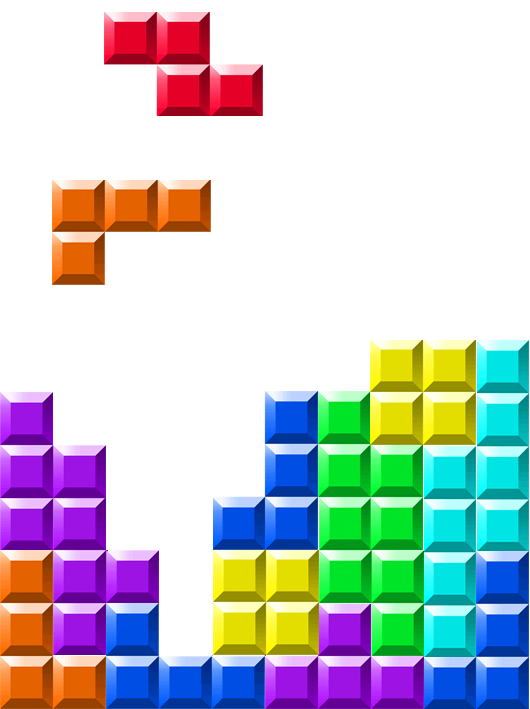
\includegraphics[width=0.25\textwidth, angle=0]{figures/MATSimBook.png} \end{center}

% ##################################################################################################################
The intense MATSim development and research during the last years has generated an extensive body of knowledge with a large number of studies, dissertations, and projects in research and practice. Time to put together all the floating pieces and contextualize them in a consistent and coherent manner as illustrated by above figure. 

There have been many authors and three editors contributing to this book. Authors come from the \gls{matsim} core team but also from the extended community. Chapters have been written by the respective software contributor or researcher whenever possible, which ensures capturing the most complete and detailed knowledge.

The book is intended to give the new \gls{matsim} user a quick start in running \gls{matsim}. It shall furthermore provide the experienced MATSim user and the MATSim developer with details on how to extend MATSim by plugging in the available modules, i.e.,\,the \glspl{contribution}, and by programming against the MATSim API to implement their own \gls{matsim} \glspl{extension}. Last, but not least, the book wants to contribute to the methodological discussion on the relatively new field of the joint microsimulation of travel demand and traffic flow, or more generally of spatial demand and its congestion generation, by compiling our conceptual insights on MATSim gained over the years.

To match its aims, the book is divided into the three parts focused on \emph{using, extending} and \emph{understanding} MATSim. \ah{beschreiben, wie man nach und nach inhaltlich tiefer geht.}

\textbf{Part I: using MATSim} ... \\
Chapter~\ref{ch:introducing} introduces the \gls{matsim} basics including its traffic flow model and the underlying co-evolutionary principle. 

Chapter~\ref{ch:lgstarted} takes the MATSim novice and shows him or her how to set up and run a basic \gls{matsim} scenario. 

Scoring is central to MATSim; a full chapter, Chapter~\ref{ch:scoring}, is thus assigned to scoring. 

At the point, when the readers are ready to set up their own real-world MATSim \gls{scenario}, Chapter~\ref{ch:scenarios} shows them the numerous scenarios that have been implemented worldwide. 

% -----------------
\textbf{Part II: extending MATSim} ... \\
Chapter~\ref{ch:modules} introduces \gls{matsim} modules and explains how to use the available modules introduced in Chapters~\ref{ch:destinationchoice} through \ref{ch:businessanalytics}. Chapter~\ref{ch:discontinued} describes modules, that have been important in the past, but whose development is discontinued.

Chapter~\ref{ch:developmentprocess} shortly describes the development process of MATSim, i.e.,\,the team and the community and their development tools are summarized. 

Chapter~\ref{ch:extensionpoints} goes one step further and explains how to write your own MATSim extension and how to later contribute it to \gls{matsim}. It details at which points MATSim can be extended, and it digs a little deeper and provides details about the very central \gls{matsim} concept of "events". How to add a \lstinline|Listener| and write a customized \lstinline|Controler| is also explained here.

% -----------------
\textbf{Part III: understanding MATSim} ... \\

\ah{etwas inhaltslos. Gunnars Überlegungen bez. Zusammenhang der Kapitel beschreiben.}

This part provides the underlying theoretical aspects of the previous two parts. For example, the \gls{matsim} score is not just a simple score denoted with $S$ anymore, but, it is here interpreted within the discrete choice framework (Chapter~\ref{ch:discretechoice}) and becomes utility denoted as common with $U$. 

But let us start, from the beginning, with the first Chapter~\ref{ch:history} providing a short summary on \gls{matsim}'s history written by the Kai Nagel, one of \gls{matsim}'s fathers. 

Chapter~\ref{ch:abta} then elaborates on agent-based traffic assignment, qualitatively contextualizes \gls{matsim} within the classical concepts. The development from statical assignment to dynamic assignment and finally agent-based assignment is focused here.  

Chapter~\ref{ch:montecarlo} continues on that by presenting \gls{matsim} as a fundamentally stochastic tool based on random distributions and suitably describable as a Monte Carlo engine. It quantitatively contextualizes MATSim within the classical concepts.

Chapter~\ref{ch:kinematicwaves} analyzes MATSim's traffic flow model in relation to kinematic waves and Chapter~\ref{ch:economicEval} provides an economic view on \gls{matsim}. 

The book is concluded by a discussion of promising research avenues (Chapter~\ref{ch:researchavenues}).

% ##################################################################################################################
\section*{Related Material}
The book is focused on the more stable aspects of MATSim application and development, while the practical issues, such as specific configurations or code details---usually being part of manuals---can be found in the MATSim user guide (shipped with the MATSim releases) and provided on the MATSim web page \citep[][]{MATSim_Userguide_2015}.

% ##################################################################################################################
 \cleardoublepage

\addtocontents{toc}{\bigskip}

\pagenumbering{arabic}

% ===========================================================================
% book body

% -----------------------
\part{Using MATSim} \cleardoublepage
\chapter{Introducing MATSim}
\kaitodo[inline]{read chapter/section}
\label{ch:introducing}
% ##################################################################################################################
\hfill \textbf{Author:} Andreas Horni, Kai Nagel, Kay W. Axhausen

\begin{center} 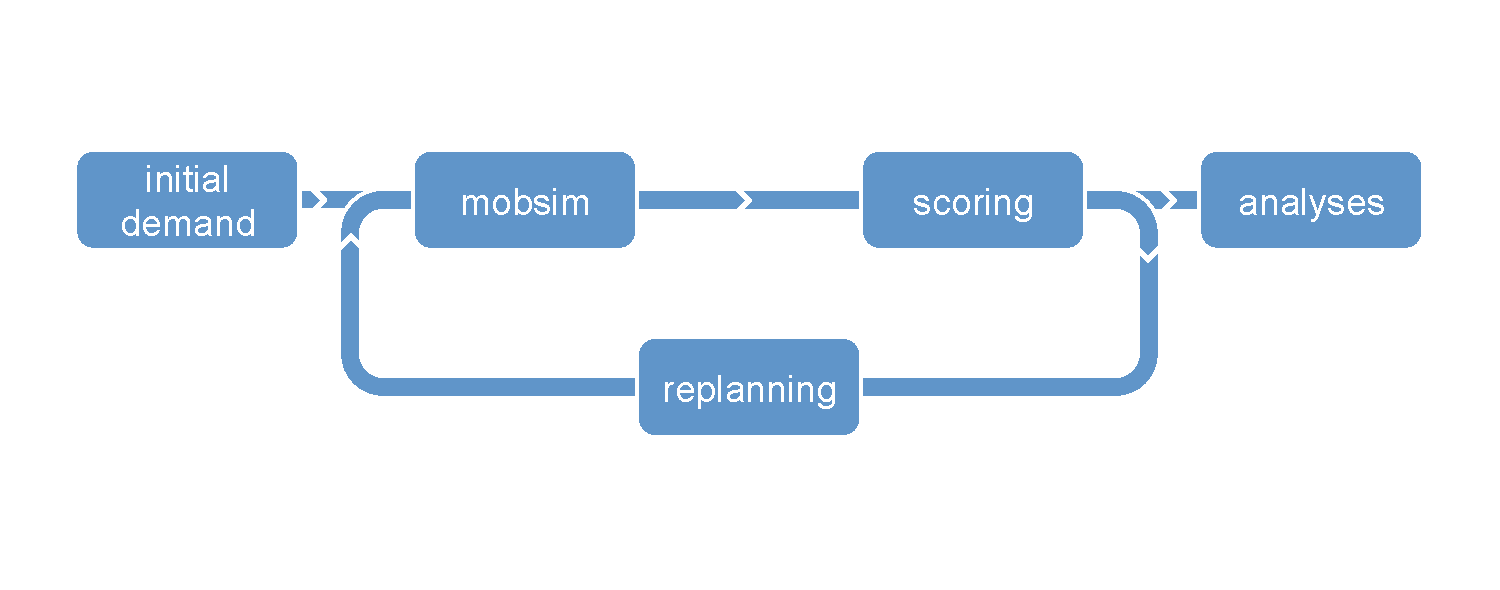
\includegraphics[width=0.7\textwidth, angle=0]{figures/matsimcycle.pdf} \end{center}

\editdone{This text has undergone the professional edit. Please no grammatical changes anymore! They are most-probably wrong.}

% ##################################################################################################################
\section{The Beginnings}
\label{sec:howitstarted}
The \gls{matsim} project \citep[][]{MATSIM_Webpage_2015} started with Kai~Nagel, then at ETH Zürich, and his interest in improving his work with, and for, the \gls{transims} project \citep[][]{SmithEtc1995TRANSIMSSeattle,TRANSIMSFHWA_Webpage_2013}; he also wanted to make the resulting code open-source.\footnote{%
%
TRANSIMS has, since then, also become open-source \citep{TRANSIMSOS_Webpage_2013}; but in 2000, it was difficult to procure in Europe.
%
} After Kai~Nagel's departure to Berlin in 2004, Kay~W.~Axhausen joined the team, bringing a different approach and experience. A collaboration---successful and productive for more than 10\,years---was thus established, combining a physicist's and a civil engineer's perspective, as well as  bringing together expertise in
%
traffic flow,
%
\gls{largescale} computation,
%
choice modeling
%
and
%
\glspl{cas}:
%
%% \st{His background in traffic flow, complex adaptive systems, and large-scale computation was complemented with experience in the agent-based modeling of travel demand when---after Kai~Nagel's departure to Berlin in 2004---Kay~W.~Axhausen joined the effort in earnest.}
%
%% \ah{Transims war doch auch schon agent-based, oder?}
%
%% \kai{Transims hatte individuelle Personen mit Plänen für Aktivitäten und Routen.  Aber die Information war über mehrere Dateien verteilt: eine für die synthetic population, eine für die activity plans, eine für die trips.  Als Resultat hatte die dynamische Umlegung z.B.\ nicht das Einkommen der Person, oder der zweite Trip eines Agenten konnte starten, bevor der erste beendet war. -- Daher war es wohl ``weniger'' agenten-orientiert als matsim.}
%
%% \st{It is this merger of two, actually three large and old streams of research, which has made the system unique from the start:}
%
%% \ah{Gilt das genauso für Transims (?), so unique war das also auf dieser Ebene beim Start nicht oder? Die Unterschiede sind eher bei "MATSim had to important differences..." (siehe unten)}
%% \ah{unique? Wie genau hängt dies mit den Strands unten zusammen. Dem Leser Zusammenhang zeigen. Reihenfolge ändern 1 $\to$ 2 ?}
%
%% \ah{transition}
%
%% As detailed in Chapter~\ref{ch:history}, about \gls{matsim}'s history, \gls{matsim} 
%% %is a merger of three large and old 
%% combines several streams of research, namely 
\begin{itemize}\styleItemize
%
\item \textbf{Microscopic modeling of traffic:} \gls{matsim} performs integral microscopic \emph{simulation of resulting traffic flows} and the congestion they produce (see Section~\ref{sec:trafficflowmodel}).
%
\item \textbf{Microscopic behavioral modeling of demand/agent-based modeling:}
%\textbf{Agent-Based Modeling:} 
  \gls{matsim} uses a microscopic description of demand by \emph{tracing the daily schedule} and the synthetic travelers's decisions.  In retrospect, this can be called ``agent-based''.
  %% \ah{Könnte man das agent-based modeling mit ``...''/ in den Bullet-Titel nehmen, wie mal als Vorschlag eingefügt? Ist ja ein zentraler Begriff für MATSim.}
  % ok.  kai, jan'15
%
\item \textbf{Computational physics:}
%% , in particular simple and thereby fast models of physical processes:} 
%% Computational physics has performed simulations with $10^8$ and more particles already in the 1980s.
\gls{matsim} performs fast microscopic simulations with $10^7$ or more ``particles''.
%
\item  \textbf{Complex adaptive systems/co-evolutionary algorithms:}
 %% and equilibrium modeling:} 
\gls{matsim} \emph{optimizes the experienced utilities} of the whole schedule through the co-evolutionary search for the resulting equilibrium or steady state (see Section~\ref{sec:co-ev}). 
%
%% \kai{Andreas, habe ``equilibrium modelling'' aus der Überschrift rausgenommen.  Ist das für irgendwen wichtig? Für mich war/ist equilibrium immer nur eine Krücke.  Eigentlich ist auch hier das entscheidende Paper \citep{ArthurBar}, welches gerade darauf hinausläuft, dass man ``coordination'' auch bekommt, ohne dass die Agenten ökonometrisch optimieren.}

\end{itemize}

%\kai{Habe an obigem nochmal rumgeschrieben. Nachdem ich die ``bullets'' dann fertig hatte, sahen sie fast genauso aus wie die bereits vorher existierende Aufzählung nach ``bringing together expertise''.}

%% \ah{changed order to make it consistent with order below (now in history)}

%% \st{The robustness of this framework for the description of all congested spatial behaviors became clear as the development progressed to include the congestion inside facilities and buildings or as parking was added.} \ah{etwas weg von Argumentationslinie?}

%% \ah{moved everything from here to history}

%In transport modeling, these streams have evolved from the 1970's for microscopic traffic flow and agent-based demand modeling \citep[e.g.,][]{Wiedemann_PhDThesis_1974, Seddon_Simulation_1972}, while transport equilibrium modeling already started in the 1950's \citep[][]{Wardrop_PICE_1952}. At the end of 1990’s the scene was set for a merger of these strands into a computationally efficient, modular and open-source software enabling further development on travel behavior, network response and efficient computation: \gls{matsim}.

At the end of the 1990’s, the scene was set for these research streams' mergence %% \todoah{\kai{Hallo Andreas, weißt Du, wo ``mergence'' herkommt?  Habe ich noch nie gehört.}}\ah{Lektorat hat aus ``merger'', ``mergence'' gemacht.} 
into a computationally 
efficient, modular, open-source software enabling further development on travel behavior, network response and efficient computation: \gls{matsim}.

% ----------------------------

%\ah{alles ab hier würde ich viel lieber in Chapter~\ref{ch:history} sehen. Hier will man doch nur ein Häppchen History um MATSim grob einordnen zu können. Ohne breites Hintergrundwissen sind nachfolgende Abschnitte nicht leicht verdaubar.}
%\ah{Würde hier einfach noch 2,3 Sätze in Richtung ... merging microscopic modeling, the agent-based approach and the notion of equilibrium ... usw.}
%\ah{und dann enden mit "At the end of 1990’s the scene was set for a merger of these strands into a computationally efficient, modular and open-source software enabling further development on travel behavior, network response and efficient computation."}
%\ah{Was meinst du? Könnte das sonst mal versuchen ...}
%\kai{Von mir aus sehr gerne.}

% ----------------------------

%% As shown on the web page \citet[][]{MATSIM-Scenarios_Webpage_2015} and detailed in Chapter \ref{ch:scenarios}, \gls{matsim} has been applied by local research groups world-wide for multiple different regions. 
%% % \ah{see Discussion~\ref{sec:matsimtd}}
%
%finde den jetzt auskommentierten Absatz arg ``out of context''.  M.E. müsste da entweder zusätzliches Text drumrum, oder wir lassen ihn weg.  Habe ihn jetzt erstmal auskommentiert.  kai, dec'14

% ##################################################################################################################
\section{In Brief}
\label{sec:inbrief}
\gls{matsim} is an activity-based, extendable, multi-agent simulation \gls{framework} 
%toolkit
%\kai{m.E.\ framework} 
implemented with 
%the current version of 
\gls{java}. It is open-source and can be downloaded from the Internet \citep[][]{MATSIM_Webpage_2015, GitHub_Webpage_2015}. The \gls{framework} is especially designed for large-scale scenarios, meaning that all models' features are stripped down to efficiently handle the targeted functionality; parallelization has also been very important \citep[e.g.,][]{Dobler_TechRep_IVT_2011, Charypar_PhDThesis_2008}. For the network loading simulation, for example, a queue-based model is implemented, omitting very complex and computationally expensive car-following behavior (see Section~\ref{sec:trafficflowmodel}).

At this time, \gls{matsim} is 
%conceptually 
%
%I don't think it is ``conceptually''.  If anything, it is just the current software. kai, jan'15
designed to model a \emph{single day}, the common unit of analysis for \gls{activitybased} models \citep[see, for example, the review by][]{Bowman_TEC_2009_1}. 
%% In other words, \gls{matsim} is currently limited to the dynamics within that day. 
Nevertheless, in principle, a 
multi-day model could be implemented \citep[][]{HorniEtAl_TechRep_IVT_2012_a}.

As shown in Section~\ref{sec:co-ev}, \gls{matsim} is based on the co-evolutionary principle. Every agent repeatedly optimizes its daily \gls{activity} schedule, while in  competition for space-time slots with all other agents on the transportation infrastructure.  This is somewhat similar to the route assignment iterative cycle, but goes beyond route assignment, by incorporating other choice dimensions like time choice \citep{BalmerRaneyEtAl2005act-times}, mode choice \citep{GretherEtAl2009SimpleModeChoiceIPL}, or destination choice %% \citep{HorniEtAl_unpub_TRB_2012} 
\citep{HorniEtAl2011TrbLocationChoice}
% taking this reference from tub.bib since the IVT version does not even contain the preprint number. kai, aug'15
into the iterative loop.
%% \kai{Andreas, fallen dir noch weitere Referenzen ein?} \ah{Ich würde sagen, dies ist die wichtigste.}

% ------------
%\begin{figure}
\createfigure%
{\protect\gls{matsim} loop, sometimes called the \protect\gls{matsim} cycle}%
{\protect\gls{matsim} loop, sometimes called the \protect\gls{matsim} cycle%% \kai{Andreas, I replaced ``execution'' by ``mobsim''.} \ah{perfect. I think, we have to do that at various other places on the webpage (?)}}%
  % oh well.  Konzentrieren wir uns erstmal auf das Buch, und darauf, dass die URLs im Buch sinnvoll und stabil sind. kai, jan'15
%, sometimes also called the "MATSim washing machine"}%
}
{\label{fig:matsimcycle}}%
{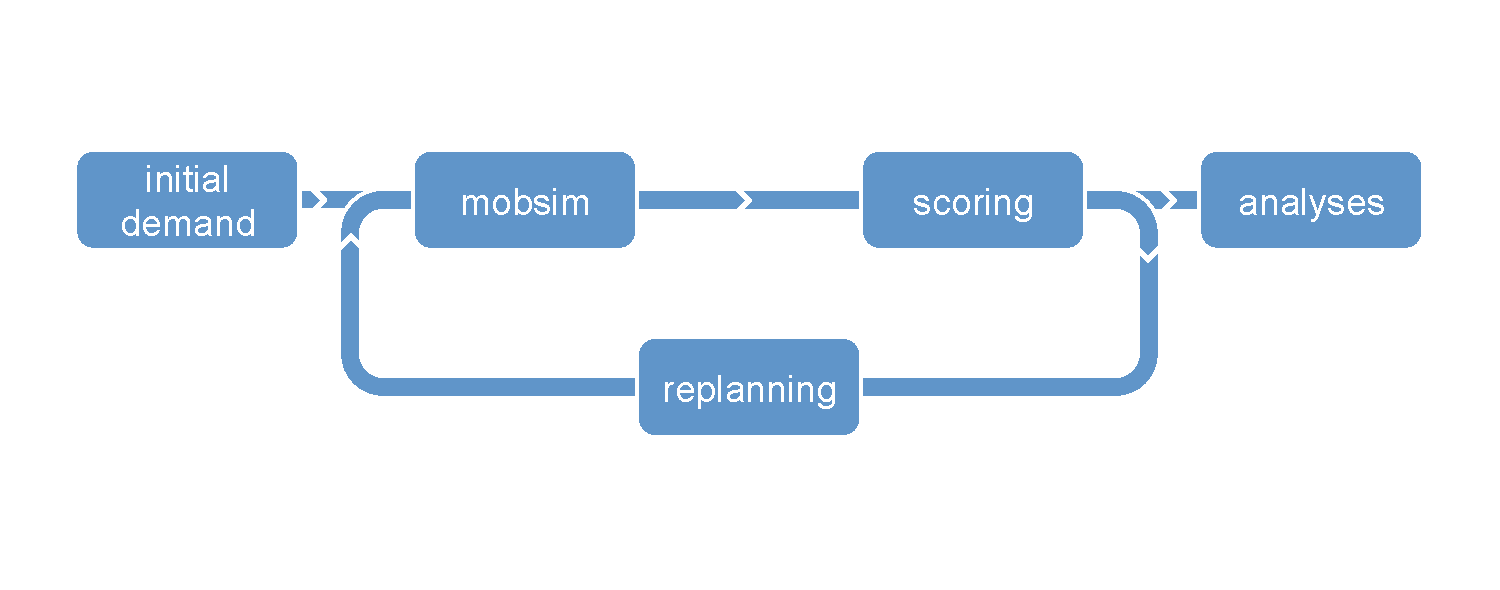
\includegraphics[width=0.99\textwidth, angle=0]{figures/matsimcycle.pdf}}%
{}
%\end{figure}
% ------------

A \gls{matsimrun} contains a configurable number of iterations, represented by the loop of Figure~\ref{fig:matsimcycle} and detailed below. 
%
It starts with an initial demand arising from the \gls{study} area population's daily activity chains. The modeled persons are called agents in \gls{matsim}. Activity chains are usually derived from empirical data through sampling or discrete choice modeling. A variety of approaches is suitable, as evidenced in the scenarios' chapters (Chapter~\ref{ch:scenarios}). During iterations, this initial demand is optimized. Every agent possesses a memory containing a fixed number of day plans, where each \gls{plan} is composed of a daily activity chain and an associated \gls{score}.  The score can be interpreted as econometric utility (\cf Chapter~\ref{ch:economicEval}).

In every iteration, prior to the simulation of the network loading with the \gls{matsim} \emph{\gls{mobsim}} \citep[e.g.,][]{Cetin_PhDThesis_2005}, each agent selects a plan from its memory. This selection is dependent on the plan \emph{scores}, which are computed after each mobsim run, based on the executed plans' performances. A certain share of the agents 
%$\varphi$ 
(often 10\,\%) is allowed to clone the selected plan and modify this clone (\emph{\gls{replanning}}).
%% With the \gls{msa} usually a decreasing share of travelers is reallocated to a new plan to avoid oscillations. For \gls{matsim}, it has been shown that a variable replanning share over the course of the iterations can be productive and \emph{"increases overall performance of the system by a factor of three or more"} \citep[][p.7f]{CharyparEtAl_IATBR_2006}.
%% \kai{Andreas, ich habe das mit dem ``decreasing share of travelers'' mal rausgenommen.  M.E.\ ist das weder im core noch in einer contrib implementiert.  Somit gehört es auf jeden Fall nicht nach ``using matsim''.  --  Es gibt einen MSA switch, aber der bezieht sich auf den score. --  Falls die Aussagen von DC im Buch vorkommen sollen, müssten sie wohl eher irgendwo nach ``understanding matsim''.} \ah{Danke!}
For the network loading 
%microsimulation % \ah{to me microsimulation is not a necessary word hier.}
step, multiple \glspl{mobsim} are available and configurable \citep[see][also see Section~\ref{sec:using-mobsims} of this book]{HorniEtAl_TechRep_IVT_2011_a}.

Plan modification is performed by the \emph{replanning} modules. Four dimensions are usually considered for \gls{matsim} at this time: departure time (and, implicitly, activity duration) \citep[][]{BalmerRaneyEtAl2005act-times}, route \citep[]{LefebvreBalmer_unpub_STRC_2007}, mode \citep{GretherEtAl2009SimpleModeChoiceIPL} and destination \citep{HorniEtAl_TRR_2009,
%HorniEtAl_unpub_TRB_2012
HorniEtAl2011TrbLocationChoice%
}. 
% taking last reference from tub.bib since the ivt bib does not even contain the
% preprint number. kai, aug'15
Further dimensions, such as activity adding or dropping, or parking and group choices are currently under development and only available experimentally. % Siehe Tabelle MATSim-Präsentationen Prof.\ Axhausen.
\gls{matsim} replanning offers different strategies to adapt plans, ranging from random mutation to approximate suggestions, to best-response answers where, in every iteration, the currently optimal choice is searched. For example, routing
%and destination replanning are
often is a best-response modification%
%(possibly taking into account ``frozen'' randomness)
, while time and mode replanning are random mutations.
%% \kai{Andreas, habe in obigem Satz locachoice rausgenommen.  (1) Echte best response ist m.E.\ technisch schwierig, weil der router nicht die genauen Reisezeiten ausspuckt.  Thibaut sieht das m.E.\ genauso.  (2) Wenn Du tatsächlich echte best response machst, dann müsste doch immer das gleiche rauskommen, es sei denn, die Reisezeiten ändern sich drastisch von einem Aufruf zum nächsten. -- Man könnte es reinnehmen, bräuchte dann aber m.E.\ auch einen Hinweis auf die frozen randomness, was für dieses frühe Kapitel vielleicht zu schwergewichtig daherkommt?} \ah{ok. Reine best response ist es ja sowieso nicht, weil ich um den Approximationsfehler im Back-wards Dijkstra zu kompensieren wieder Probs bei der provisorischen Auswahl reingenommen habe.}

Initial day chains do not have to be very carefully defined for the replanning dimensions included in the optimization process. Plausible values just speed up the optimization process. 

If an agent ends up with too many plans (configurable), the plan with the lowest score (configurable) is removed from the agent's memory. Agents that have not undergone replanning select between existing plans. The selection model is configurable; in many \gls{matsim} investigations, a model generating a logit distribution for plan selection is used.

An iteration is completed by evaluating agents' day experience of the selected day plans (\emph{scoring}). The applied scoring function is described in detail in Chapter \ref{ch:scoring}.

% ------------
\createfigure[t]%
{Typical score progress}%
{Typical score progress}%
{\label{fig:scoreprogress}}%
{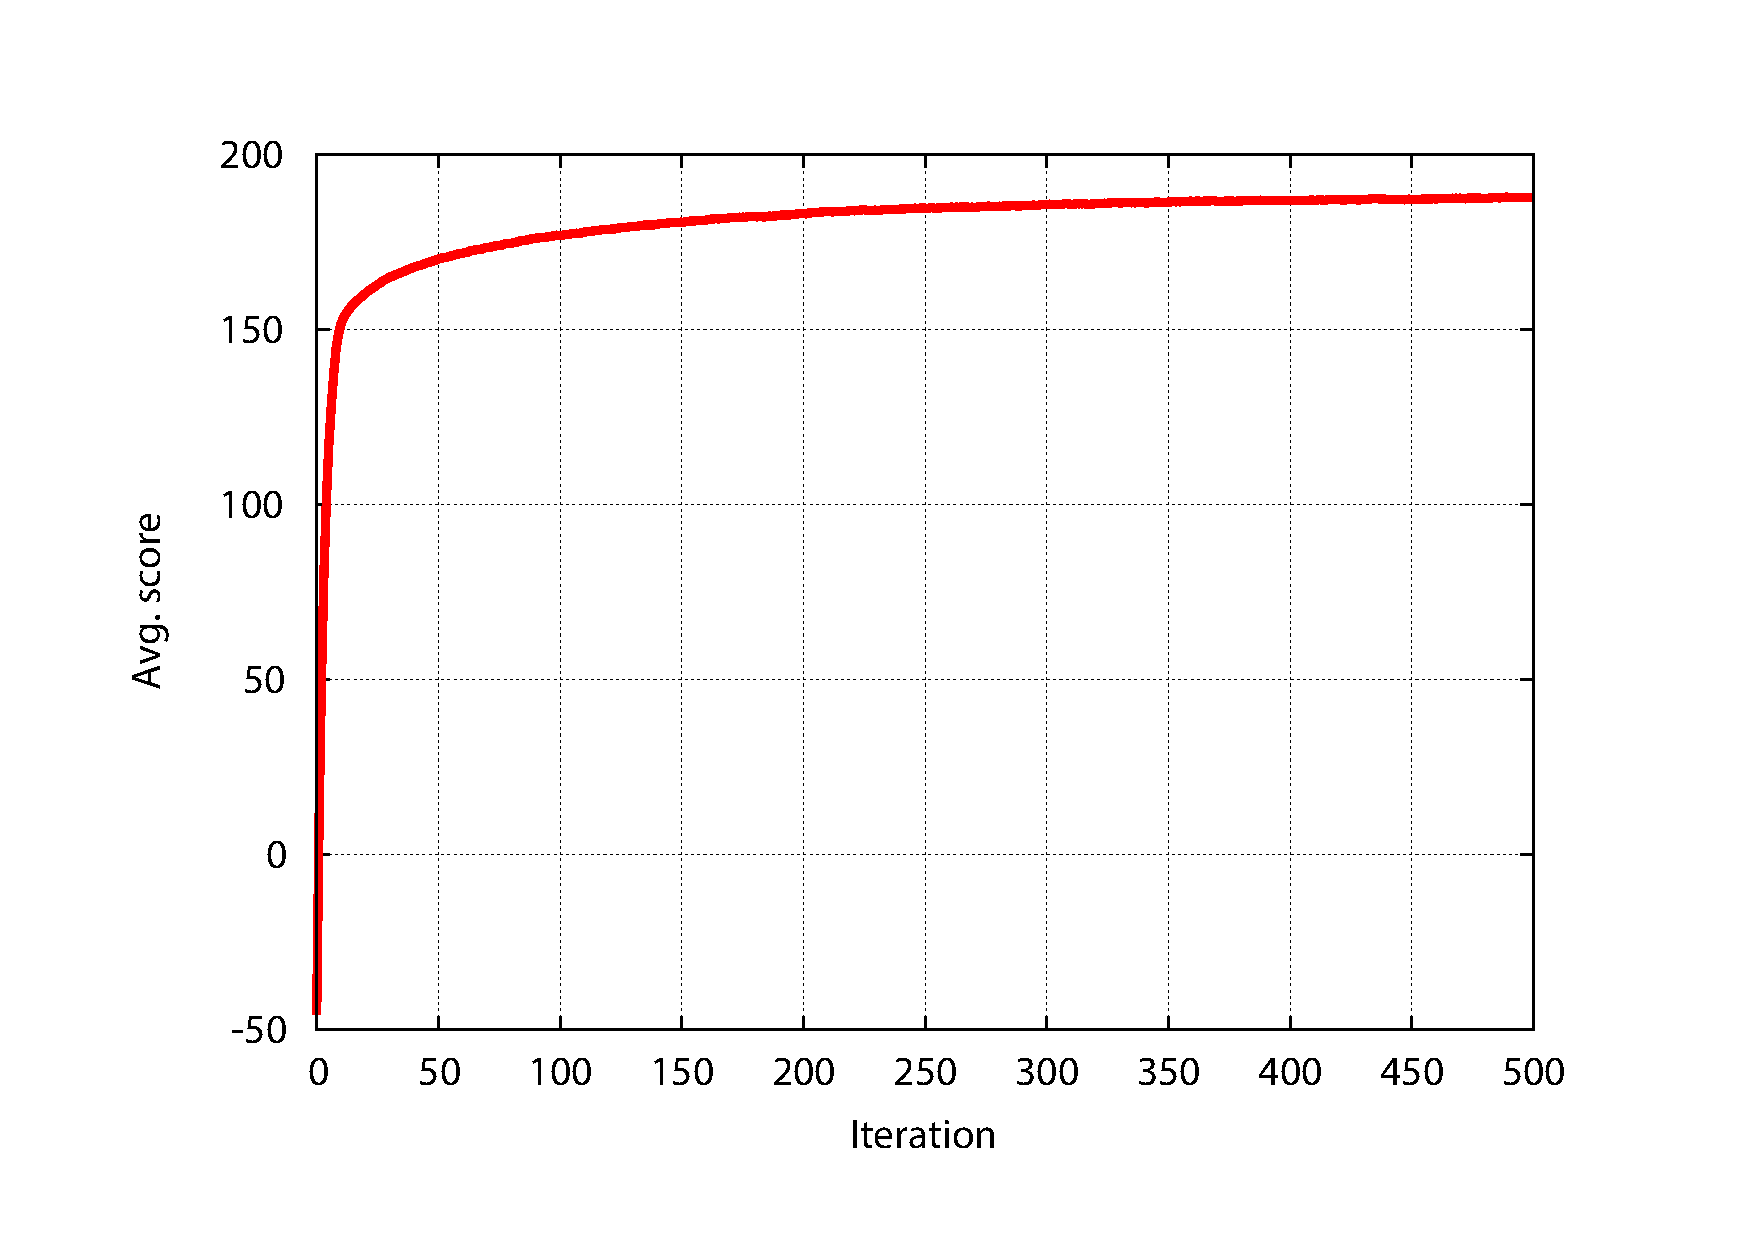
\includegraphics[width=0.99\textwidth, angle=0]{using/figures/scores.pdf}}%
{}
% ------------

The iterative process is repeated until the average population score stabilizes.
%% , where the definition of the stopping criterion is subject of research initialized by \citet[][]{Meister_PhDThesis_2011, NagelFloetteroed2009IatbrResourceInBook}.
The typical score development curve \citep[Figure~\ref{fig:scoreprogress}, taken from][]{HorniEtAl_TRR_2009} takes the form of an evolutionary optimization progress \citep[][Figure~2.5]{EibenSmithJE_2003}.  Since the simulations are stochastic, one can not use convergence criteria appropriate for deterministic algorithms; for a discussion of possible approaches for the \gls{matsim} situation, see Chapters~\ref{sec:score-convergence} and \ref{sec:Relaxation-as-a} as well as \citet{Meister_PhDThesis_2011}.

\gls{matsim} offers considerable customizability through its modular design. Although %replacing
implementing alternative core modules, such as an alternative network loading simulation, may entail substantial effort,
% \citep[][Section 2.4]{MATSim_Userguide_2015} \todokai{rm usrguide}, 
in principle, every module of the framework can be exchanged. \gls{matsim} modules are described in Chapter~\ref{ch:modules} and following.

\gls{matsim} is strongly based on events stemming from the \gls{mobsim}. Every action in the simulation generates an event, which is recorded for analysis. These event records can be aggregated to evaluate any measure at the desired resolution. The event architecture is detailed in Section~\ref{sec:events-extension-point}.

% ##################################################################################################################
\section{MATSim's Traffic Flow Model}
\label{sec:trafficflowmodel}
\gls{matsim} provides two internal \glspl{mobsim}: \gls{qsim} and \gls{jdeqsim} and external mobility simulations can be plugged in. Some years ago, the \gls{deqsim} written in \gls{cpp} and described by \citet[][]{Charypar_PhDThesis_2008,%
%% CharyparEtAl_TRR_2007,%
CharyparAxhausenEtAl2007Event-DrivenQueueBasedTraffic,%
%CharyparEtAl_WCTRS_2007,%
CharyparAxhausenEtAl2007event-drivenparallelqueue-based,%
CharyparEtAl_TRB_2009}
was plugged into \gls{matsim} and frequently used. The multi-threaded \gls{qsim} is currently the default \gls{mobsim}.
 %% \citep[][]{MATSim_Userguide_2015}. \todokai{rm usrguide}% commit 29999 michaz

\citet[][]{CharyparEtAl_TRB_2009} distinguishes between 
\begin{itemize}\styleItemize
\item physical simulations, featuring detailed car following models, %\ah{I have changed simulations for microsimulation}
\item cellular automata, in which roads are discretized into cells,
\item queue-based simulations, where traffic dynamics are modeled with waiting queues,
\item mesoscopic models, using aggregates to determine travel speeds, and
\item macroscopic models, based on flows rather than single traveler units (\eg cars).
\end{itemize}

As \gls{matsim} is designed for large-scale \glspl{scenario}, it adopts the computationally efficient queue-based approach (see Figure~\ref{fig:queue}). A car entering a network link (\ie a road segment) is added to the tail of the waiting queue. It remains there until the time for traveling the link with free flow has passed and until he or she is at the head of the waiting queue and until the next destination link allows entering. The approach is very efficient, but clearly it comes at the price of reduced resolution, \ie car following effects are not captured.   
%
\createfigure%
{Traffic flow model}%
{Traffic flow model}%
{\label{fig:queue}}%
{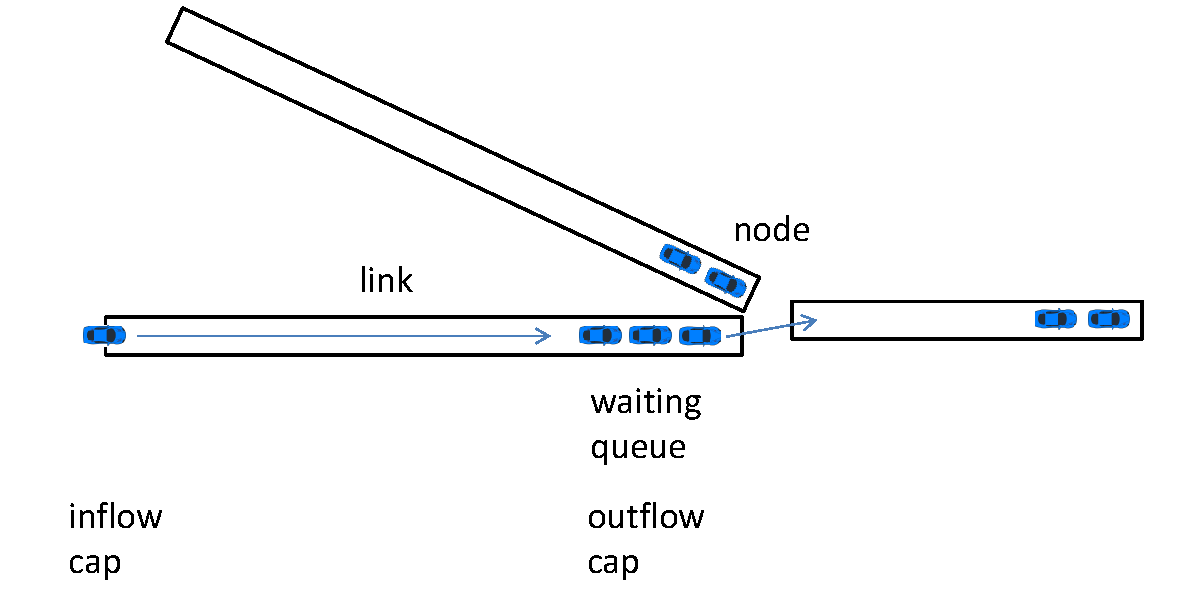
\includegraphics[width=0.9\textwidth, angle=0]{using/figures/queue.pdf}}%
{}
%
In \gls{jdeqsim}, for computational reasons, the waiting-queue approach is combined with an event-based update step \citep[][]{CharyparEtAl_TRB_2009}. In other words, there is no time-step-based updating process of any agent in the scenario. Instead agents are only touched if they actually require an action. For example, links do not have to be processed while agents traverse them.
%% an agent needs to pass a link (i.e., he or she is waiting in the queue), he or she does not need to be processed.
%
%"and agent (that) needs to pass a link" wird auch in der normale QSim nicht angefasst.  ALLERDINGS fasst die normale QSim Kanten an, auf denen Agenten unterwegs sind ... selbst wenn wir wissen, dass sie frühestens in einer Stunde rauskommen können. kai, jan'2015
%
%\kai{Ich kriege Ärger, wenn agents immer nur männlich sind.  Ist kein Witz; wurde mir bei meinen ersten öffentlichen Auftritten in Berlin sehr deutlich bedeutet.}  
% \ah{korrigiert}
Update events triggering is managed by a global scheduler. \gls{qsim}, however, is time-step based. 
%\ah{see Discussion~\ref{sec:scenariod}}
%
%\kai{Aber in der QSim ist das nicht so; die ist ganz normal time-stepped.  Sie schaltet nur Kanten ab, die nicht ``aktiv'' sind.} 
%
% \ah{korrigiert}
%
The \gls{matsim} traffic flow model is strongly based on the two link attributes: storage capacity and flow capacity. Storage capacity defines the number of cars fitting onto a network link.
%% It is a physical property and thus fixed in the simulation.
%
%% \kai{Andreas, I removed the statement ``it is a physical property and thus fixed in the simulation'' ... network change events können die Anzahl der Fahrspuren und damit die storage capacity verändern.} \ah{ok}
%
%% For scenarios with a population smaller then the full population, say a 10\% sample, however, it needs to be scaled down, since otherwise there will be no spill-back any more.

Flow capacity specifies the outflow capacity of a link, \ie how many travelers can leave the respective link. 
It is an individual attribute of the link.  
In current implementations, there is no \emph{maximum} inflow capacity specified.
The many simulation experiments with \gls{qsim} (and the former \lstinline|queueSimulation|) have shown that neglecting \emph{maximum} inflow capacity does not have a substantial effect, but further reduces model complexity. 
In the earlier \gls{deqsim} and current \gls{jdeqsim}, a \emph{minimum} inflow capacity can also be specified to capture breakdowns at link entries \citep[][p.~99]{Charypar_PhDThesis_2008}.

This basic traffic flow model has been extended with various modules; signals and multiple lane modeling have been added (Chapter~\ref{ch:signalslanes}), 
backward-moving gaps, as investigated by \citet[][]{Charypar_PhDThesis_2008}, are included in \gls{jdeqsim}, but only available on an \emph{experimental base} for \gls{qsim} (Section\ref{sec:researchavenues-double-queue-mobsim}). 
Interactions between different modes are described in Section~\ref{sec:using-othermodesthancar} and Chapter~\ref{ch:multimodalsim}. 
% \ah{This is not correct anymore as far as I know. signals+lanes contrib and qsim passingQ}
%Limitations of the traffic flow model concern link dynamics (in particular overtaking and slow drivers) 
% and intersection dynamics (in particular turn restrictions not explicitly modeled in the network). 

% ##################################################################################################################
\section{MATSim's Co-Evolutionary Algorithm}
\label{sec:co-ev}
%
% ------------
\createfigure[!h!t!]%
{The co-evolutionary algorithm in \protect\gls{matsim}}%
{The co-evolutionary algorithm in \protect\gls{matsim}%
%% \kai{Andreas, warum ist beim allgemeinen co-evolutionary algorithm die interaction nicht bei der `fitness evaluation'?}
%% \ah{Mhhhm, Ort war abiträr gedacht, sollte einfach die Interaktion zwischen den Spezies zeigen. Habs jetzt raufgeschoben.}
%
}%
{\label{fig:ea}}%
{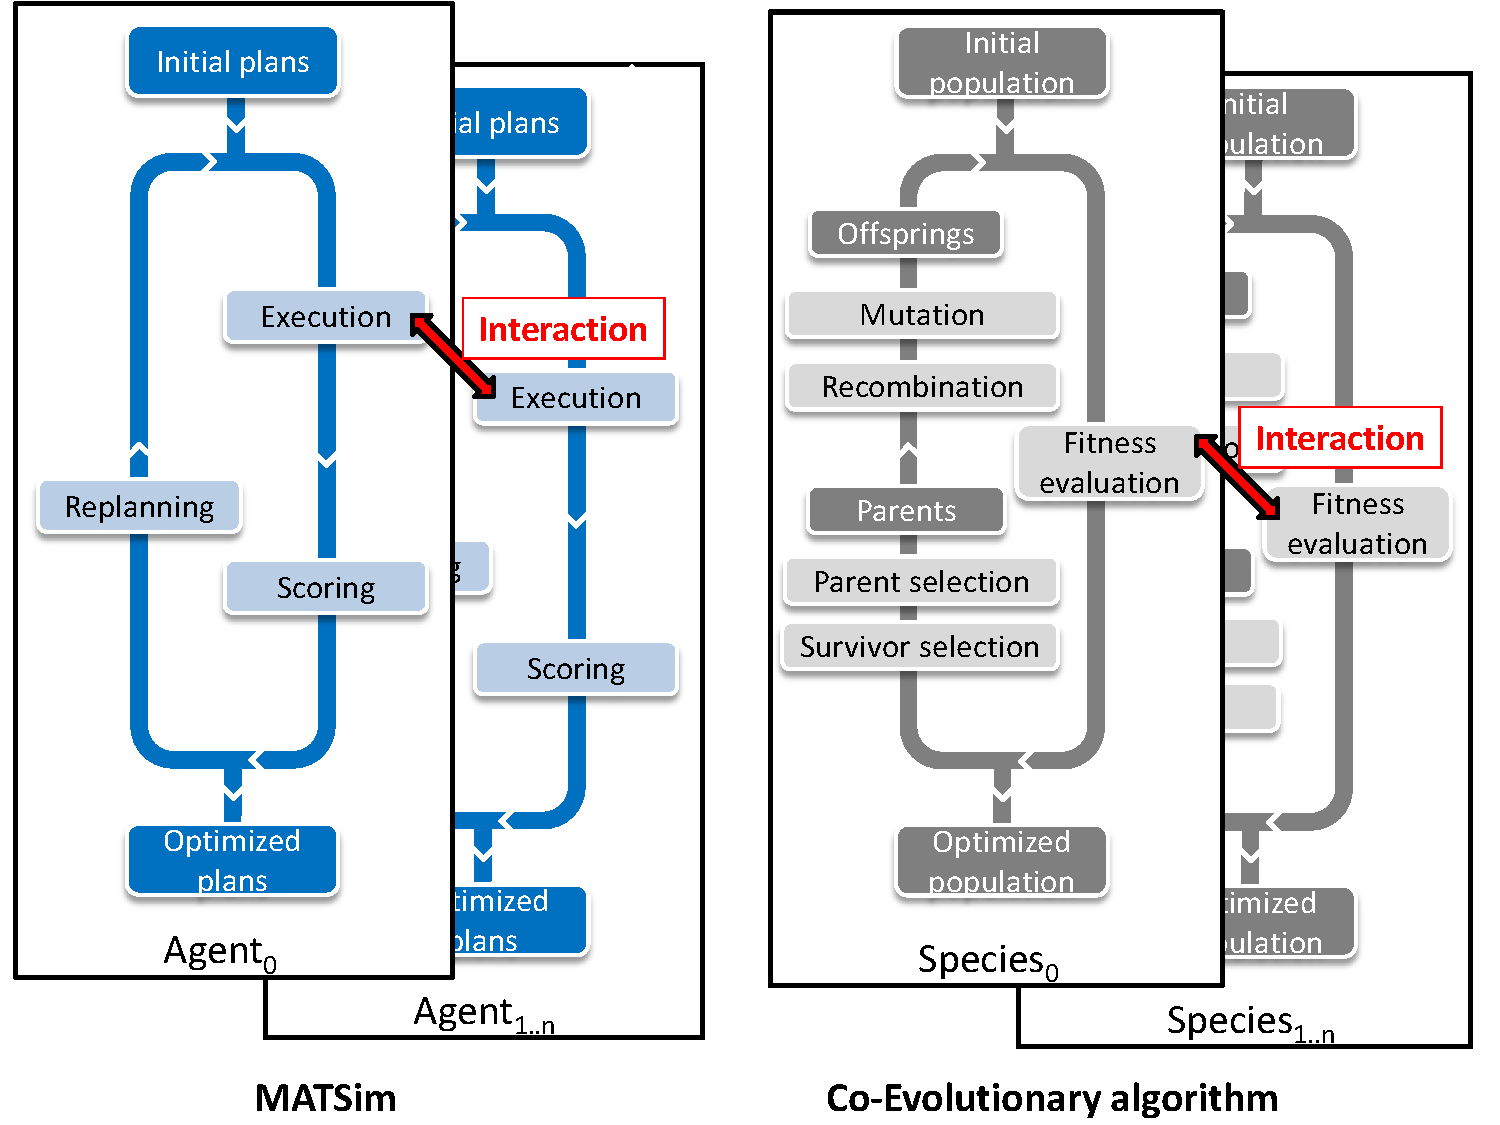
\includegraphics[width=0.99\textwidth, angle=0]{using/figures/MATSimVSea.pdf}}%
{}
% ------------
%
%\kai{Nett.  Gibt es eine Quelle für den ``co-evolutionary algorithm''?} \ah{fürs Bild? Hab ich mir selber aus den Fingern gesogen. Für Co-EAs allgemein?} \thibaut{du kannst \cite{PopoviciEtAl_2012} %gucken, find ich sehr gut. zum mindesten benutze ich immer diese in meine Papers}
%
As illustrated in Figure~\ref{fig:ea}, the \gls{matsim} equilibrium is searched by a \emph{\index{co-evolutionary algorithm}} \citep[see e.g.,][]{PopoviciEtAl_2012}. These \glspl{algorithm} co-evolve different species subject to interaction (\eg competition). In \gls{matsim}, individuals are represented by their plans, where a person represents a species. With the co-evolutionary algorithm, optimization is performed in terms of agents' plans , \ie across the whole daily plan of activities and travel. It achieves more than the standard traffic flow \glspl{equilibrium}, which ignores activities. Eventually, an equilibrium is reached, subject to constraints, where the agents cannot further improve their plans unilaterally. 

%Strictly speaking, 
Note that there is a difference between application of an evolutionary algorithm and a \emph{co}-evolutionary algorithm. An evolutionary algorithm would lead to a system optimum, as optimization is applied with a global (or population) fitness function. Instead, the co-evolutionary algorithm leads to a (stochastic) user \gls{equilibrium}, as optimization is performed in terms of \emph{individual} scoring functions and within an agent's set of plans. 
%% At the moment, the \gls{matsim} co-evolutionary algorithm only includes mutation; recombination may come into play when coordinated day plans of family members, for example, are included in the future.
%
% einschränkende (und damit negative) Bemerkung, die m.E. an dieser Stelle nicht zwingend ist: genetische Algorithmen haben wohl etwas mit cross-over zu tun, evolutionäre (als Oberbegriff) aber nicht.  kai, jan'15

% ##################################################################################################################
%\section{Discussions}
% =============================================================================================
%\subsection{MATSim-T, MATSim-F, MATSim}
%\label{sec:matsimtd}
%
%\kai{Wie gesagt, ich wäre gegen ``MATSim-T'' und für einfach nur ``MATSim''.  Siehe \url{http://matsim.org/conceptual-meeting/2012/notes}.}
%
%\kai{
%Bei einem der meetings (m.E. conceptual, aber es mach auch developer gewesen sein) gab es mal eine Diskussion, ob wir die Bezeichnung "toolbox" wirklich beibehalten wollen.
%
%Wir waren uns damals einig, dass matsim eher ein framework als eine toolbox ist.
%
%(ca. 30 vs. ca. 3 hits auf matsim.org)
%
%Inzwischen, mit den "scripts-in-java", weicht das langsam ein wenig auf.  Aber wir hatten damals eigentlich beschlossen, sowohl auf "-T" als auch auf "-F" zu verzichten.
%
%(Wir brauchen einen "Stadtschreiber", damit wir uns an solche Diskussionen erinnern. :-) )
%
%Sollten wir das dann nicht auch im "Buch" machen?  Gibt es Personen, die an dem "-T" hängen?
%
%}
%
%\ah{erledigt}

% =============================================================================================
%\subsection{Scenario}
%\label{sec:scenariod}
%\kwaah{We should add at the start that 'scenario' is the combination of case study data (population size, initial plans, networks and facilities), policies, the selected replanning modules and the selected traffic flow simulation.} 
%
%\kai{I have to admit that I have that differently in my head.  
%%
%In the code, scenario is only the first, and this is also how I always had it in my own head: The ``XXX'' scenario is a collection of files.  
%%
%Selected \gls{replanning} \glspl{module} and selected traffic flow simulation is config; a sceanrio preferably comes together with a config that makes it runnable, but it is a different thing.  
%%
%And policy is policy; essentially the difference between (base case scenario | base case config) and (policy case scenario | policy case config).  
%%
%All three things together are a study for me.} 
%
%
%\kai{Wobei ``scenario'' so wie hier im ursprünglichen Text benutzt m.E.\ stehen bleiben kann.}
%%
%
%\kwaah{
%Kai, 
%
%I have no problem either way, but see many text where the inclusive use is implied. 
%
%But i am happy to see it split into 
%
%Scenario: population plans networks facilities
%
%Config = modules switched on
%
%Policies
%
%It is just that in many contexts in planning "Scenario" is equal to experiment or run. If we are consistent fine
%
%Kay
%}
%
%\kai{
%oh weh.  So etwas wie "the considered policy scenario is the large-scale introduction of autonomous vehicles in Los Angeles County"? 
%
%Vielleicht können wir 
%
%(1) versuchen, "policy scenario" und "(matsim) scenario" erstmal auseinander zu halten
%
%(2) es im Auge zu behalten, ob uns eine bessere Lösung einfällt.
%%
%...
%%
%Ich lese übrigens gerade nochmal (kleine) Teile des (großen) Buches von Russell/Norvig (Introduction to AI, a modern approach).  Da gibt es "utility based agents" ... 
%
%... aber "An agent's utility function is essentially an internalization of the performance measure."
%
%\textbf{\textit{Hier ist als "utility" nicht gleich "econometric utility"}}.
%}
%
%
%\kai{
%Im Satz davor:
%
%"a \textbf{performance measure} assigns a \textbf{score} to any given sequence of environment states"
%
%Ein Unterschied scheint zu sein, dass das eher von außen gesehen wird, also das, was bei uns das Systemoptimum ist. 
%
%Das liegt (m.E.) daran, dass "software agents" eher als Hilfsmittel zur Problemlösung gesehen werden; man versucht als, deren utility function so zu wählen, dass insgesamt der gewünschte Systemzustand rauskommt.
%
%Hier weichen "agent-based systems" (im Sinne von mechanism design) also von "agent-based simulation" (im Sinne von "Modell der Wirklichkeit") voneinander ab.
%}
%
%\kwaah{
%Danke, Kai
%
%das sprachliche Monster ist ein Unding fuer den Alltag: (MATSim) scenario und policy run koennte vielleicht helfen. 
%
%Die Frage nach score, utility, objective function ist genauso schwierig. Vielleicht sollten wir in den ersten beiden Teilen  von ‘score’ oder ‘objective function’ sprechen und erst in Teil 3 von utility
%
%Kay
%}
%
%\gunnar{Ich weiss nicht, ob es hilft: Ich habe bislang "scenario" als "sufficient set of boundary conditions to execute the simulation" verstanden und "configuration" dann als dessen technische Spezifikation.
%}

% ##################################################################################################################
\ifthenelse{\boolean{printBibPerChapter}}{\bibpc}{}

% ##################################################################################################################
% Local Variables:
% mode: latex
% mode: reftex
% mode: visual-line
% TeX-master: "../main"
% comment-padding: 1
% fill-column: 9999
% End: 
 \cleardoublepage
\chapter{Let's Get Started}
\label{ch:lgstarted}
% ##################################################################################################################
\hfill \textbf{Authors:} ..., Andreas Horni, Marcel Rieser, ...

\begin{center} 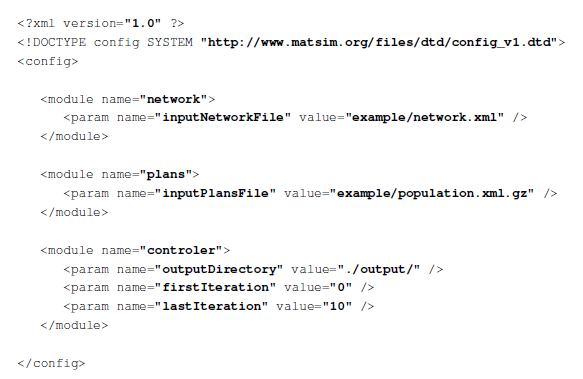
\includegraphics[width=0.7\textwidth, angle=0]{using/figures/config.png} \end{center}

% ##################################################################################################################
This chapter explains how to set up and run MATSim and it describes the requirements of building a basic scenario. As this book tries to be as stable and timeless as possible, the MATSim user guide \citep[][]{MATSim_Userguide_2014} needs to be consulted in addition to this chapter for doing an actual installation; frequently changing and detailed information such as download paths or version-dependent configurations are omitted here and left to the user guide. 

Getting the source code into different computing environments and extending MATSim through the API is described in the second part of the book in Chapter~\ref{ch:extensionpoints}.

% ##################################################################################################################
\section{Running MATSim}
\label{sec:runningmatsim}

% ================================================================================================
\subsection{Setting Up MATSim}
To run MATSim you have to install the Java Platform Standard Edition (SE) that complies with the MATSim version to be run. At the time of writing this book, this is JAVA SE 7.

Furthermore you need the official MATSim release, which comes as a zip file (usually named with the version number \lstinline|matsim-yy.yy.yy.zip|) including everything that is required to run it. It can be downloaded following the links on the MATSim web page. Unzip it and continue with Section~\ref{sec:runexample}.

If you prefer to use the more up to date nightly builds, you need to manually download the matsim jar file (usually named with the revision number \lstinline|MATSim_ryyyy.jar|) and the required external libraries (\lstinline|MATSim_libs.zip|). Unzipping this collection of 3rd-party libraries, you should then get a directory \lstinline|libs| with several jar-files inside. If the directory \lstinline|libs| is in the same directory as the MATSim jar-file, the libraries are found automatically and does not have to be added to the \lstinline|classpath| manually.

% ================================================================================================
\subsection{Running MATSim}
\label{sec:runexample}

\kai{note: inzwischen kann man auch einfach auf das matsim jar draufklicken. :--)  Das sollten wir unbedingt nochmal testen, und dann beschreiben.  (Geht nicht mit dem derzeitigen release 6, aber im HEAD und nightly builds geht es schon.)}

MATSim does not provide a graphical user interface, thus, you need to be able to handle and access a command line tool. In Linux or Mac OS X, this is typically a Terminal application, and in Windows, the Power Shell or Command Prompt.

On the command prompt type the following command as one line, but substitute the correct paths: 

\lstinline|java -Xmx512m -cp /path/to/matsim.jar org.matsim.run.Controler /path/to/config.xml|

As an example, on Linux this could look like: \\
\lstinline|java -Xmx512m -cp /home/username/matsim/matsim.jar org.matsim.run.Controler /home/user/matsim/input/config.xml|

On Mac OS X, it could look like this: \\
\lstinline|java -Xmx512m -cp /Users/username/matsim/matsim.jar org.matsim.run.Controler /Users/user/matsim/input/config.xml|

On Windows, an example command could be: \\
\lstinline|java -Xmx512m -cp C:\MATSim\matsim.jar org.matsim.run.Controler C:\MATSim\input\config.xml|

Such a command exists of multiple parts:
\begin{compactitem}
\item \lstinline|java| tells the system that you want to run Java.
\item \lstinline|-Xmx512m| tells Java that it should use up to 512 MB of memory. This is typically enough to run the small examples. For larger scenarios, you might need more memory, e.g., \lstinline|-Xmx3g| would allow Java to use up to 3 GB of memory.
\item \lstinline|-cp /path/to/matsim.jar| tells Java where to find the MATSim code.
\item \lstinline|org.matsim.run.Controler| specifies which class (think of an ``entry point'') should be run. In most cases, the default MATSim Controler is the class you'll need to run simulations.
\item \lstinline|/path/to/config.xml| tells MATSim which config file is to be used.
\end{compactitem}

% ================================================================================================
\subsection{Configuring MATSim}
Configuring MATSim is (at this stage) only done via the configuration file, often just referred to as \lstinline|config file| or as \lstinline|config.xml|. It builds the connection between the user and MATSim. It contains a list of settings which influence how the simulation behaves. In the second part of the book we will learn how MATSim can be configured and extended by programming against its API.

All configuration parameters are simple pairs of a parameter \lstinline|name| and a parameter \lstinline|value|. The parameters are grouped into logical groups. For example, there is a group with settings related to the Controler like the number of iterations, or there is another group with settings related to the simulation, e.g.\ the end time of the simulation. As shown in Chapter~\ref{ch:modules}, a whole bunch of MATSim modules can be added to MATSim and configured by specifying the respective section of the configuration file.

The list of available parameters and valid parameter values may vary from release to release. Although we try to keep this stable, due to changes in the software, most notably by new features, settings may change. To get a list of all available settings currently available, run the following command: \lstinline|java -cp matsim.jar org.matsim.run.CreateFullConfig fullConfig.xml|.

This command will create a new config file \lstinline|fullConfig.xml|, which contains the full list of available parameters along with their default values. This makes it easy to see what settings are available. To use and modify certain settings, the lines with the corresponding parameters can be copied to the config file specific for the scenario to be simulated and the parameter values be modified in that file. 

A minimal configuration file is shown below, specifying the minimal information that MATSim needs about demand and supply. In the example, supply is given by the network and demand is given in the plans file (typical input data produced is described in Section \ref{sec:inputdata}). Please note that MATSim does nothing else for this case than running the mobility simulation, i.e., no replanning of the demand is performed.

\begin{xml}
<?xml version="1.0" ?> 
<!DOCTYPE config SYSTEM "http://www.matsim.org/files/dtd/config_v1.dtd"> 
<config> 
 
   <module name="network"> 
      <param name="inputNetworkFile" value="example/network.xml" /> 
   </module> 
 
   <module name="plans"> 
      <param name="inputPlansFile" value="example/population.xml.gz" /> 
   </module> 
</config>
\end{xml}

% ##################################################################################################################
\section{Building and Running a Basic Scenario}
\label{sec:buildingbasicscenario}
% ===============================================================================================
This section provides information on the typical input data files used for a MATSim experiment, and the standard output files generated. It presents a parsimonious example scenario and shortly explains units, conventions and coordinate systems used in MATSim. Finally some hints on practical data requirements and how to perform calibration, verification and validation are given.

% ===============================================================================================
\subsection{Typical Input Data}
\label{sec:inputdata}
Minimally MATSim needs the files
\begin{compactitem}
	\item \lstinline|config.xml|, containing the configuration options for MATSim and presented above,
	\item \lstinline|network.xml|, with the description of the (road) network, and
	\item \lstinline|population.xml|, providing information about	the travel demand, i.e., the list of agents and their day plans.
\end{compactitem}
%
With this setting, MATSim agents perform their activities on a specific link. If further information about activity locations needs to be specified, this can be done in 
\begin{compactitem}
\item \lstinline|facilities.xml|. 
\end{compactitem}
%
If MATSim facilities are used, the agents perform their activities in a specific facility attached to a network link.

In the beginning of MATSim only car mode could be simulated. With the addition of the public transport module (Chapter~\ref{ch:pt}), with the help of two further input files public transport can just as well be simulated:
\begin{compactitem}
\item \lstinline|transitVehicles.xml| providing the description of the vehicles used for public transport services. 
\item \lstinline|transitSchedule.xml| containing information about transit stop locations and transit services,
\end{compactitem}
%
For the handling of other modes please refer to Chapter~\ref{ch:multimodalsim}.

Count data are the common evaluation measure in transport planning. In MATSim count data can be integrated with the file
\begin{compactitem}
\item \lstinline|counts.xml| containing hourly volumes from real-world counting stations.
\end{compactitem}

Some of the files, especially \lstinline|population.xml|, but also \lstinline|network.xml| or \lstinline|facilities.xml|, might get quite large. To save space, MATSim supports reading and writing the data in a compressed format. MATSim uses GZIP-compression for this. Thus, in many cases, the file names have the additional suffix \lstinline|.gz|, as in \lstinline|population.xml.gz|. MATSim automatically detects if files are compressed or should be written compressed based on the filename. 

In more detail the input files look as follows. Note that the configuration file is presented above.

% -----------------------------------------------------------------------
\subsubsection{network.xml}
The network describes the infrastructure on which the agents (or the vehicles, respectively), can move around. The network consists of nodes and links (in graph theory, these are typically called vertices and edges). A simple example for a description of a network in MATSim's XML data format can look as follows.

\begin{xml}
<?xml version="1.0" encoding="utf-8"?> 
<!DOCTYPE network SYSTEM "http://www.matsim.org/files/dtd/network_v1.dtd"> 
 
<network name="example network"> 
   <nodes> 
      <node id="1" x="0.0" y="0.0"/> 
      <node id="2" x="1000.0" y="0.0"/> 
      <node id="3" x="1000.0" y="1000.0"/> 
   </nodes> 
   <links> 
      <link id="1" from="1" to="2" length="3000.00" capacity="3600" 
                                 freespeed="27.78" permlanes="2" modes="car" /> 
      <link id="2" from="2" to="3" length="4000.00" capacity="1800" 
                                 freespeed="27.78" permlanes="1" modes="car" /> 
      <link id="3" from="3" to="2" length="4000.00" capacity="1800" 
                                 freespeed="27.78" permlanes="1" modes="car" /> 
      <link id="4" from="3" to="1" length="6000.00" capacity="3600" 
                                 freespeed="27.78" permlanes="2" modes="car" /> 
   </links> 
</network>
\end{xml}

Each element has an identifier id. Nodes are described by an \lstinline|x| and a \lstinline|y| coordinate value. Links have more attributes: The \lstinline|from| and \lstinline|to| attribute reference nodes and describe the geometry of the network. Additional attributes describe the traffic-related aspects of the network:
\begin{compactitem}
    \item the \lstinline|length| of the link, typically in meters (see Section~\ref{sec:unitsconventions}).
    \item the flow \lstinline|capacity| of the link, i.e.\ the number of vehicles that can pass the link, typically in vehicles per hour.
    \item the \lstinline|freespeed| is the maximum speed at which vehicles are allowed to travel along the link, typically in meters per seconds.
    \item the number of lanes (\lstinline|permlanes|) available in the direction specified by the from and to nodes.
    \item the list of \lstinline|modes| allowed on the link. This is a comma-separated list, e.g.\ \lstinline|modes="car,bike,taxi"|.
\end{compactitem}
Note that all links are uni-directional. If a road can be traveled in both directions, two links have to be defined with alternating \lstinline|to| and \lstinline|from| attributes (see links with id 2 and 3 in the example given in the lsiting above). Thus, the network can be seen as a directed graph. 

% -----------------------------------------------------------------------
\subsubsection{population.xml}
The travel demand for MATSim is described by the agents' day plans. The full set of agents is typically the population, hence the filename \lstinline|population.xml|. Alternatively, \lstinline|plans.xml| is also commonly used in MATSim, as the population file essentially contains a list of day plans.

The population contains the data in a hierarchical structure as shown in the following small example.

\begin{xml}
<?xml version="1.0" encoding="utf-8"?> 
<!DOCTYPE population SYSTEM "http://www.matsim.org/files/dtd/population_v5.dtd"> 
<population> 
   <person id="1"> 
      <plan selected="yes" score="93.2987721"> 
         <act type="home" link="1" end_time="07:16:23" /> 
         <leg mode="car"> 
            <route type="links">1 2 3</route> 
         </leg> 
         <act type="work" link="3" end_time="17:38:34" /> 
         <leg mode="car"> 
            <route type="links">3 1</route> 
         </leg> 
         <act type="home" link="1" /> 
      </plan> 
   </person> 
   <person id="2"> 
      <plan selected="yes" score="144.39002"> 
         \ldots 
      </plan> 
   </person> 
</population>
\end{xml}

The population contains a list of persons, each person contains a list of plans and each plan contains a list of Activities and Legs.

Exactly one plan per person is marked as selected. The selected plan of each agent is the plan that gets executed by the mobility simulation. During the replanning stage, a different plan might get marked as being selected. A plan can contain a score as attribute. The score gets calculated and stored in the plan during the scoring stage, after the plan was executed by the mobility simulation.

The list of activities and legs in each plan describe the planned actions by each agent. Activities have a type assigned and have---except for the last activity in a day plan---an end time defined (There are some exceptions where activities have a duration instead of an end time. Such activities are often automatically generated by routing algorithms and are thus not described in this guide). To describe the location where an activity takes place, the activity is either assigned a coordinate by giving an \lstinline|x| and \lstinline|y| attribute value, or has a link assigned which describes from which link the activity can be reached. As the simulation requires the link attribute, the \lstinline|Controler| calculates the nearest link for a given coordinate in the case the attribute is missing and only an \lstinline|x| and \lstinline|y| coordinate value is given or any activity.

Legs describe how agents plan to travel from one location to the next one. Each leg must have a transport mode assigned. Optionally, legs may have an attribute \lstinline|trav_time| which describes the expected travel time for this leg. For a leg to be simulated, it must contain a route. The format of a route depends on the mode of a leg. For car-legs, the route lists the links that the agent has to travel along in the given order, while for transit-legs information about the stop locations and expected transit services are stored.

An agent starts a leg directly after the previous activity (or leg) has ended. Depending on the mode, the mobility simulation might handle the agent differently. By default, car- and transit-legs are well-supported by the mobility simulation. If the mobsim encounters a mode it does not know, it defaults to teleportation: In this case, the agent is removed from the simulated reality, and after the leg's expected travel time has passed, re-inserted at the agent's target location.

The population data format is one of the most central data structures in MATSim and might be a bit overwhelming at first. Luckily, to get started, only a small subset must be known of it. Following liusting shows how a minimal population file could look like. 

\begin{xml}
<?xml version="1.0" encoding="utf-8"?> 
<!DOCTYPE population SYSTEM "http://www.matsim.org/files/dtd/population_v5.dtd"> 
<population> 
   <person id="1"> 
      <plan> 
         <act type="home" x="5.0" y="8.0" end_time="08:00:00" /> 
         <leg mode="car" /> 
         <act type="work" x="1500.0" y="890.0" end_time="17:30:00" /> 
         <leg mode="car" /> 
         <act type="home" x="5.0" y="8.0" /> 
      </plan> 
   </person> 
   <person id="2"> 
      ... 
   </person> 
</population>
\end{xml}

Most notably, the following simplifications can be made:
\begin{compactitem}
\item Each person needs exactly one plan.
\item The plan does not need to be selected or have a score.
\item Activities can be located just by their coordinates.
\item Activities should have a somewhat meaningful end-time.
\item Legs only need a mode, but no routes.
\end{compactitem}
When a simulation is started, MATSim's \lstinline|Controler| will load such a file and then automatically assign the nearest link to each activity and calculate a suitable route for each leg. This makes it easy to get started quickly. 

% -----------------------------------------------------------------------
\subsubsection{facilities.xml}
In the facilities file location attributes can be specified. Importantly, open times and capacities can be added here. Facilities are not a mandatory element of core MATSim. Some modules, such as the destination choice module (Section~\ref{ch:destinationchoice}), use it, however.

An example listing is as follows.
\begin{xml}
<?xml version="1.0" encoding="UTF-8"?>
<!DOCTYPE facilities SYSTEM "http://www.matsim.org/files/dtd/facilities_v1.dtd">
<facilities name="test facilities for triangle network">
	<facility id="1" x="60.0" y="110.0">
		<activity type="home" />
	</facility>
	<facility id="10" x="110.0" y="270.0">
		<activity type="education" />
	</facility>
</facilities>
\end{xml}

% -----------------------------------------------------------------------
\subsubsection{transitVehicles.xml}
To simulate public transport in MATSim, two additional input files are necessary. One is \lstinline|transitSchedule.xml|, which describes the vehicles which serve the lines: are they big buses, small buses, trains or light rail vehicles, and describes how many passengers each vehicle can transport.

The description of public transport vehicles can be split into two parts: In a first part, vehicle types have to be described, specifying how many passengers such a vehicle can transport (Note that the term ``vehicle'' can refer to multiple vehicles in reality, e.g.\ a train with several wagons should be specified as one long vehicle with a high number of seats). In the second part, actual vehicles have to be listed. Each vehicle has an identifier and is of a previously specified vehicle type. The following shows an example of a such a file, describing one vehicle type and two vehicles of that type. 

\begin{xml}
<?xml version="1.0" encoding="UTF-8"?> 
<vehicleDefinitions xmlns="http://www.matsim.org/files/dtd" 
       xmlns:xsi="http://www.w3.org/2001/XMLSchema-instance" 
       xsi:schemaLocation="http://www.matsim.org/files/dtd 
                     http://www.matsim.org/files/dtd/vehicleDefinitions_v1.0.xsd"> 
	<vehicleType id="1"> 
      <description>Small Train</description> 
      <capacity> 
         <seats persons="50"/> 
         <standingRoom persons="30"/> 
      </capacity> 
      <length meter="50.0"/> 
   </vehicleType> 
   <vehicle id="tr_1" type="1"/> 
   <vehicle id="tr_2" type="1"/> 
</vehicleDefinitions>
\end{xml}

% -----------------------------------------------------------------------
\subsubsection{transitSchedule.xml}
The second file that is required to simulate public transport is \lstinline|transitSchedule.xml|, a rather complex file. It contains information about stop facilities (these can be bus stops, train stations or other stop locations) and transit services.

In the first part, the stop facilities need to be defined, giving each one a coordinate, an identifier and a reference to a link in the network. The stop can only be served by vehicles driving on that specified link. Optionally, it is possible to specify a name for the stop and if other vehicles are blocked when a transit vehicle is waiting at a stop. This last attribute is useful to model e.g.\ the difference of bus stops, where one bus stop has a bay, while at another stop, the bus has to stop on the actual road.

After the stop facilities, the transit lines, their routes and schedules are described. This is a hierarchical data structure: Each line can have one or more routes, each route has a route profile, a network route and a list of departures. Following listing represents an example of a minimalistic but complete transit schedule.

\begin{xml}
<?xml version="1.0" encoding="UTF-8"?> 
<!DOCTYPE transitSchedule SYSTEM "http://www.matsim.org/files/dtd/transitSchedule_v1.dtd"> 
<transitSchedule> 
   <transitStops> 
      <stopFacility id="1" x="990.0"  y="0.0"   name="Adorf" 
                                                linkRefId="1" isBlocking="false"/> 
      <stopFacility id="2" x="1100.0" y="980.0" name="Beweiler" 
                                                linkRefId="2" isBlocking="true"/> 
      <stopFacility id="3" x="0.0"    y="10.0"  name="Cestadt" 
                                                linkRefId="3" isBlocking="false"/> 
   </transitStops> 
   <transitLine id="Blue Line"> 
      <transitRoute id="1"> 
         <description>Just a comment.</description> 
         <transportMode>bus</transportMode> 
         <routeProfile> 
            <stop refId="1" departureOffset="00:00:00"/> 
            <stop refId="2" arrivalOffset="00:02:30" departureOffset="00:03:00" 
                                                     awaitDeparture="true"/> 
            <stop refId="3" arrivalOffset="00:05:00" awaitDeparture="true"/> 
         </routeProfile> 
         <route> 
            <link refId="1"/> 
            <link refId="2"/> 
            <link refId="3"/> 
         </route> 
         <departures> 
            <departure id="1" departureTime="07:00:00" vehicleRefId="12"/> 
            <departure id="2" departureTime="07:05:00" vehicleRefId="23"/> 
            <departure id="3" departureTime="07:10:00" vehicleRefId="34"/> 
         </departures> 
      </transitRoute> 
   </transitLine> 
</transitSchedule>
\end{xml}

Each transit line must have a unique id. Each transit route has an id which must be unique within that one line, so the same route id can be used with different lines. The \lstinline|transportMode| describes on which links in the network the line runs (Actually, this is currently not yet enforced. It would be possible to let a bus run on train links in the simulation. It might be enforced in the future).

The \lstinline|routeProfile| describes the stops this route serves, while route itself describes the series of links in the network the transit vehicle's driver has to drive along (thus often referred to as network route. Note that the complete route, i.e.\ all links the vehicle drives along, must be listed in the route, and not only the ones where stops are located. All the specified stops should occur along this route in the specified order. The time offsets given for each stop in the \lstinline|routeProfile| describe the relative time offset to an actual departure time. If a bus is to depart at 7 o'clock in the morning, and stop 2 has a \lstinline|departureOffset| of 00:03:00, this must be read that the bus is expected to depart at 07:03 at the specific stop. All stops in the route profile must have a departure offset defined, except the last one. All stops, except the first one, can optionally have an arrival offset defined. This is mostly useful for large trains that stop for several minutes at a station to help the routing algorithm to find connecting services at the correct time, namely the expected arrival time of the train.

As last part of the description of a transit route, the list of departures should be given. Each departure has an id, which must be unique within the route, and gives the departure time at the first stop of the specified route profile. In addition, the departure specifies with which vehicle the service should be run. This vehicle must be defined in the aforementioned list of transit vehicles. 

Because of its complexity, transit schedules often contain little mistakes that will return in an error when the simulation runs. Typical examples include that the network route is missing a link, or that the network route does not pass at all the defined stops in the right order. To make sure a schedule does not have any such issues before the simulation is started, a special validation routine is available:

\begin{lstlisting}
java -Xmx512m -cp /path/to/matsim.jar  
      org.matsim.pt.utils.TransitScheduleValidator  
      /path/to/transitSchedule.xml /path/to/network.xml
\end{lstlisting}

If run, this validator will print out a list of errors or warnings, if any are found, or show a message that the schedule appears to be valid. 

% -----------------------------------------------------------------------
\subsubsection{counts.xml}
MATSim provides funtionality to compare traffic volumes from your simulation to real world values. The Counts infrastructure allows to compare the traffic volumes on links on an hourly basis. The following listing shows an example of a \lstinline|counts.xml| input file required to do traffic count comparisons. 

\begin{xml}
<?xml version="1.0" encoding="UTF-8"?> 
<counts xmlns:xsi="http://www.w3.org/2001/XMLSchema-instance" 
        xsi:noNamespaceSchemaLocation="http://matsim.org/files/dtd/counts_v1.xsd" 
        name="test" desc="test counting stations" year="2014"> 
   <count loc_id="2" cs_id="005"> 
      <volume h="1" val="10.0"></volume> 
      <volume h="2" val="1.0"></volume> 
      <volume h="3" val="2.0"></volume> 
      <volume h="4" val="3.0"></volume> 
      <volume h="5" val="4.0"></volume> 
      <volume h="6" val="5.0"></volume> 
      <volume h="7" val="6.0"></volume> 
      <volume h="8" val="7.0"></volume> 
      <volume h="9" val="8.0"></volume> 
      <volume h="10" val="9.0"></volume> 
      <volume h="11" val="10.0"></volume> 
      <volume h="12" val="11.0"></volume> 
      <volume h="13" val="12.0"></volume> 
      <volume h="14" val="13.0"></volume> 
      <volume h="15" val="14.0"></volume> 
      <volume h="16" val="15.0"></volume> 
      <volume h="17" val="16.0"></volume> 
      <volume h="18" val="17.0"></volume> 
      <volume h="19" val="18.0"></volume> 
      <volume h="20" val="19.0"></volume> 
      <volume h="21" val="20.0"></volume> 
      <volume h="22" val="21.0"></volume> 
      <volume h="23" val="22.0"></volume> 
      <volume h="24" val="23.0"></volume> 
   </count> 
</counts>
\end{xml}

It starts with a header containing general descriptive information about the counts, including a year to describe how current the data is. Next, for each link having real world counts data, the hourly volumes can be specified. The network-link is referenced by the \lstinline|loc_id| attribute, in the example, it's link 2. The attribute \lstinline|cs_id| (counting station identifier) can be used to store an arbitrary description of the counting station. Most often it is used to note the original real word counting station to simplify future data comparison. The hourly volumes, specified by the hour of the day (counting starts with hour ``1'') and its value, are optional: That is, not for every hour a value must be given. If for a counting station data is only available for certain hours of the day (e.g.\ only during peak hours) it is possible to omit the other hours from the XML listing. 

% ===============================================================================================
\subsection{Typical Output Data}
\label{sec:outputdata}
MATSim creates a bunch of output data, which can be used to analyze the results but also to monitor the correct working of the current simulation setup. Some of the files are created once for a run, others are created for every iteration and for some (typically for the large ones, such as the population) the output frequency can be specified in the config file. The text files, which are created once per run, are created on the fly such that a continous monitoring of the run is possible. There are data, that are created by default (such as the score files) and there are ones, which need to be triggered by a respective configuration file section (such as count data). All output data goes to the output folder, which can be specified in the \lstinline|controler| section of the config file.

The following output data is generated.

\kai{Sollten wir (1) den Unterschied zwischen ``main'' und ``ITERS'' directory beschreiben, und (2) darauf hinweisen, wo die folgenden Dateien jeweils sind?}

\paragraph{Events:} Every action in the simulation is recorded as a so-called MATSim event, be it the starting of an activity or the change of a network link. Each \lstinline|Event| hosts one or multiple attributes. By default, the time when the \lstinline|Event| occurred is contained. Additionally, information like the id of the agent who caused the event or the id of the link where the \lstinline|Event| occurred could be included.  By default, the MATSim simulation module creates a so called Events-file in every 10th iteration. This file contains every single \lstinline|Event| that has been created by the simulation. The events file is thus a formidable base for post-analyses for example with the visualizers. Events are discussed in detail in Section~\ref{sec:events-extension-point}.

\paragraph{Log File:}
During each MATSim run, a log file is created. This file contains several information, that you might need later for your analyses. Additionally, it might be very helpful, if a run has crashed for some unknown reason. 


\paragraph{Warnings and Errors Log File:}
Sometimes, MATSim recognizes problems in the simulation or the configuration of it. It will then write warnings and errors to the log file. As the log file contains a lot of information, such warnings might get overlooked. For this reason, a separate log file is generated in the output directory of a run containing only warnings and error messages. It is advised to have a look during/after a run into this file to see if there have been any major problems.

\paragraph{Score Statistics:}
Once per run the score statistics are printed out. They are available as picture (\lstinline|scorestats.png|) as well as a text file (\lstinline|scorestats.txt|). They show the average best, worst, executed and average of all plans of an agent for every iteration. An example score plot is shown in Figure~\ref{fig:scoreprogress}.

\kai{``run'' vs ``iterations'': Wir benutzen normalerweise die Semantik, dass ein ``run'' die Summe aller ``iterations'' ist.  Dann wäre das oben ``Once per iteration''.  Oder ``At the end of each run'', obwohl das technisch nicht richtig ist, weil es tatsächlich am Ende einer jeden Iteration neu erzeugt wird; so kann man alles bereits während der Iterationen mitverfolgen.}

\paragraph{Leg Travel Distance Statistics:}
Also once per run, leg travel distance statistics are generated. They are comparable to the score statistics, but instead of the score, the travel distance is plotted. The files are named \lstinline|traveldistancestats.png| and \lstinline|traveldistancestats.txt|.

\kai{dto}

\paragraph{Stopwatch:}
Once per run, timing information is printed. The stopwatch file (\lstinline|stopwatch.txt|) contains the durations of actions like the replanning or the execution of the mobility simulation for every iteration. This data might be helpful for performance analyses (e.g.\ how long does the replanning take compared to the mobility simulation?).

\kai{dto}

\paragraph{Leg Histogram:}
In every iteration, a leg histogram is plotted. A leg histogram depicts the number of agents that arrive, depart or are en route per time unit. Histograms are created for each transport mode and, additionally, for the sum of all transport modes. Each file starts with the iteration number and ends with the transport mode (e.g.\ \lstinline|1.legHistogram_car.png| or \lstinline|1.legHistogram_all.png|). Moreover, a text file is created (e.g.\ \lstinline|1.legHistogram.txt|) that contains the data for all transport modes.

\paragraph{Trip Durations:}
Per iteration, a trip durations text file (e.g.\ \lstinline|1.tripdurations.txt|) listing the number of trips and their durations on a time bin level for each activity pair (e.g.\ from work to home or from home to shopping) is put out.

\paragraph{Link Volumes:}
The printing of the link volume comparison (between simulated and counted volumes) needs to be triggered by a config file entry. The comparison generates overview summaries for the whole netwoek but also analyses for individual links. A link analysis might like like Figure~\ref{fig:countcomparison}.

% ----------
\createfigure%
{Example for a Link Volumes Comparison Between Simulation and Road Count Values}%
{Example for a Link Volumes Comparison Between Simulation and Road Count Values}%
{\label{fig:countcomparison}}%
{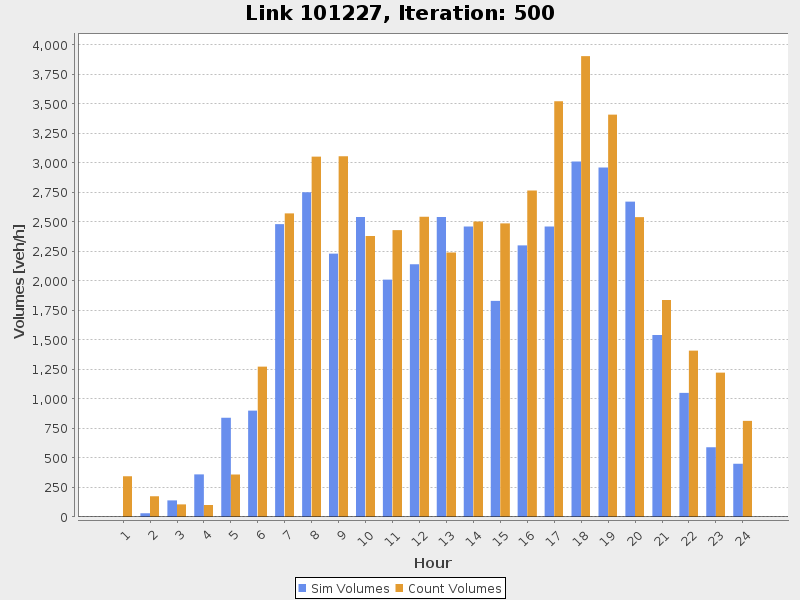
\includegraphics[width=0.7\textwidth, angle=0]{using/figures/link101227.png}}%
{}
% ----------

\paragraph{kmz:}

\kai{??}


% ===============================================================================================
\subsection{An Example Scenario}
The MATSim release is shipped with an example scenario named \lstinline|equil| in the folder \lstinline|examples/equil|. The scenario contains the following files \lstinline|config.xml|, \lstinline|network.xml| and \lstinline|plans100.xml| containing 100 persons with their day plans, one using public transport, the other person using car mode \kai{100 or 2 persons?}. Additional populations containing only 2 persons (\lstinline|plans2.xml|) or 2000 persons are provided (\lstinline|plans2000.xml.gz|). Furthermore, an example for count data can be found in the folder (\lstinline|counts100.xml|). 

%% or trips with taxi mode is also provided (\lstinline|plans-w-taxi.xml|). 

%% A tolls file can be used for road pricing scenarios not discussed here (\lstinline|toll.xml|).


\kai{Habe da neulich, als Resultat einer Diskussion, etwas ausgedünnt.  Müssen wir ggf.\ anpassen, aber m.E.\ stimmt es so nun.}

There is also a file with a demand of exactly 100 \emph{trips} (\lstinline|plans100trips.xml|), i.e.\ demand just going from one location to another, using a \lstinline$dummy$ activity type at each end.  This is provided to show that \acrshort{matsim} can also be run as a fully trip-based approach.  Clearly, it loses some of its expressiveness, but the basic concepts, including route and even departure time adaptation, still work in exactly the same way.

The network of the scenario is shown in Figure~\ref{fig:equil}.

% ----------
\createfigure%
{Equil Scenario Network}%
{Equil Scenario Network}%
{\label{fig:equil}}%
{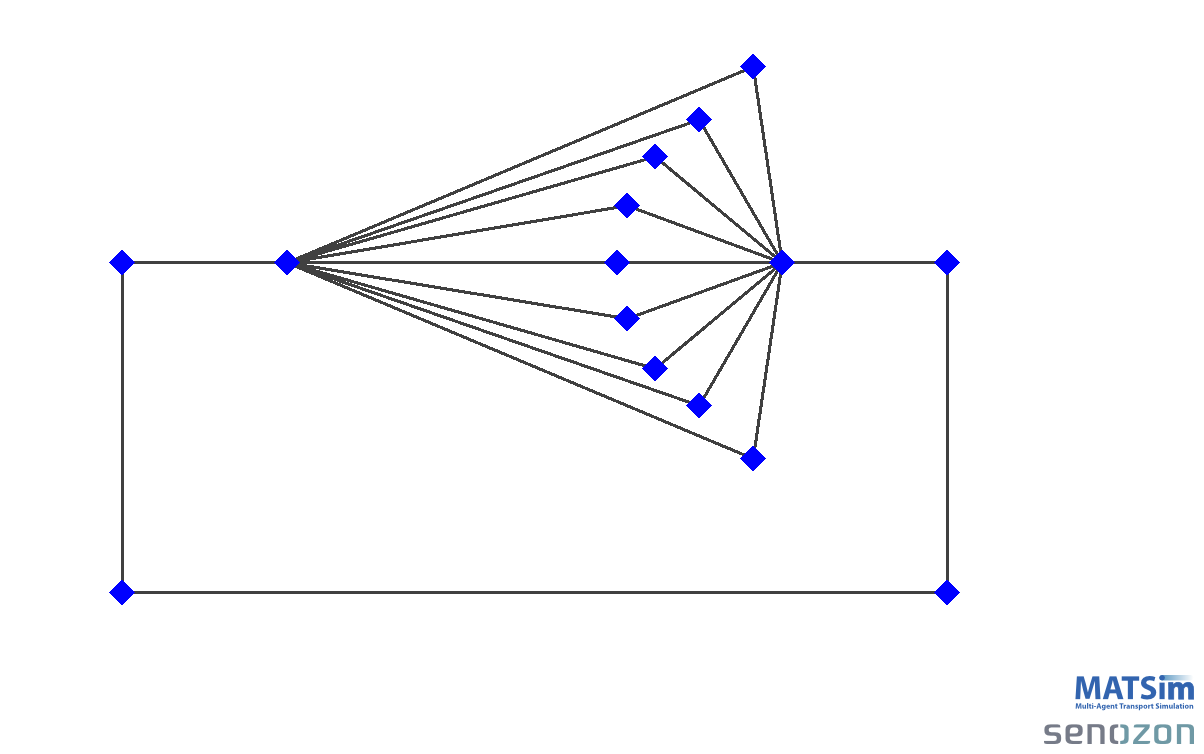
\includegraphics[width=0.8\textwidth, angle=0]{using/figures/equil.png}}%
{}
% ----------

The following lines explain the scenario by picking the most important sections from the config file \lstinline|config.xml|.

As shown in the listing below, this scenario uses replanning. 10\% of the agents reroute their current route (module \lstinline|ReRoute|). The remaining 90\% select their highest score plan for reexecution in the current iteration (module \lstinline|BestScore|). Plans get deleted from the agent's memeory if it is full defined by \lstinline|maxAgentPlanMemorySize|. By default, the plan with the lowest score is removed, while this is configurable and currently subject of intense reserach (see Section~\ref{sec:choicesets}).
%
\begin{xml}
<module name="strategy">
	<param name="maxAgentPlanMemorySize" value="5" /> <!-- 0 means unlimited -->

	<param name="ModuleProbability_1" value="0.9" />
	<param name="Module_1" value="BestScore" />

	<param name="ModuleProbability_2" value="0.1" />
	<param name="Module_2" value="ReRoute" />
</module>
\end{xml}

\kai{I think there is a better syntax for the above now (without the numbering); should we use that?}

The section \lstinline|planCalcScore| defines the parameters used for scoring. The parameters are explained in Chapter~\ref{ch:scoring}. As can be seen in the example the two activity types \lstinline|h| (home) and \lstinline|w| (work) are specified. The scenario is run for 10 iterations, writes the output files to \lstinline|./output/equil| (Section~\ref{sec:outputdata}), and uses \lstinline|qsim| as the mobility simulation (more on \gls{mobsim}s in Section~\ref{sec:trafficflowmodel} and \ref{sec:mobsims}).

\begin{xml}
<module name="controler">
	<param name="outputDirectory" value="./output/equil" />
	<param name="lastIteration" value="10" />
	<param name="mobsim" value="qsim" />	
</module>
\end{xml}

\kai{I would suggest to say something about via already at this point.  There is a free educational version so I think that this would be ok.}

% ===============================================================================================
\subsection{Units, Conventions and Coordinate Systems}
\label{sec:unitsconventions}
% ----------------------------------------------------------------------------
\subsubsection{Units}
MATSim tries to make as few assumptions about actual units as is possible, but at some locations it cannot be done without any. In general, MATSim expects similar values (e.g.\ all distances) to be in the same unit wherever they are used. In the following, the most important (expected) units are listed in a short overview. 

\paragraph{Distance}

Distance units are most prominently used in links' length. They should be specified in the same unit that the coordinate system uses. This allows MATSim to use simple triangulation, e.g.\ with the nodes' coordinates, to calculate beeline distances. As most of the typically used, projected coordinate systems (see Section~\ref{sec:coordinatesystems}) use meters as unit of distance, this is the most common used unit of distance in MATSim. 

\paragraph{Time}

While MATSim supports an hour:minute:second notation in several places, internally it uses seconds as the default time unit. This implies that for example link speeds must be specified in distance per second, typically m/s. One notable exception from this rule are scoring parameters, where MATSim expects values per hour. This is due to the fact that most behavioral parameters like value of time are typically estimated per minute or hour, and that the corresponding values for seconds are very small and thus error prone to be configured. 

\paragraph{Money}

Money is unit-free.  The units are implictly given by the marginal utility of money (cf.\ Equation~(\ref{eq:tdisutility}).  That is when, say, one moves from Germany to Switzerland, then the parameter $\beta_c$ has to be changed from ``utility per Euro'' to ``utility per Swiss franc''.

% ----------------------------------------------------------------------------
\subsubsection{Conventions}
MATSim makes heavy uses of identifiers, short \lstinline|Id|s. This Ids can be arbitrary strings, with the following exceptions: Ids should not contain any spaces (incl. tabs, new lines, etc) or commas, as those characters are typically used for separating different Ids from each other in Id lists. 

% ----------------------------------------------------------------------------
\subsubsection{Coordinate Systems}
\label{sec:coordinatesystems}
\paragraph{Preparing Your Data in the Right Coordinate System:}
In several input files, you need to specify coordinates, e.g.\ for the nodes of the network. It is strongly suggested not to use WGS84 coordinates (i.e.\ GPS coordinates, or any other kind of spherical coordinates; coordinates ranging from -180 to +180 in west-east direction, and from -90 to +90 in south-north direction). MATSim needs to calculate distances between two points in several places of the code. The calculation of distances between spheric coordinates is very complex and potentially slow. Instead, MATSim uses the simple Pythagoras' theorem, but this requires the coordinates to be in a Cartesian coordinate system. Thus is is stronlgy advised to use a Cartesian coordinate system along with MATSim, preferably one where the distance unit corresponds to one meter.

Many countries and regions have custom coordinate system defined, optimized for usages in their apropriet areas. It might be best to ask some GIS specialists in your region of interest what the most commonly used local coordinate system is and use that as well for your data.

If you don not have any clue about what coordinate system is used in your region, it might be best to use the Universal Transverse Mercator coordinate system. This coordinate system divides the world into multiple bands, each six degrees width and separated into a northern and southern part, which it calls UTM zones. For each zone, an optimized coordinate system is defined. Choose the UTM zone which covers your region (Wikipedia has a nice map showing the zones) and use its coordinate system. 

\paragraph{Telling MATSim about Your Coordinate System:}
In some places, MATSim requires to know which coordinate system your data is in. You have multiple ways to specify the coordinate system you use. The easiest one is to use the so-called ``EPSG codes''. Most of the commonly used coordinate systems got standardized and numbered. The EPSG code uniquely identifies a coordinate system and can be directly used by MATSim. As an alternative, MATSim can also parse the description of a coordinate system in the so-called WKT format. As the WKT format is much more error prone it is suggested to use EPSG codes whenever possible.

To find the correct EPSG code for your coordinate system (e.g.\ for one of the UTM zones), the website \url{http://www.spatialreference.org} is of great use. Search on this website for your coordinate system, e.g.\ for ``WGS84 / UTM Zone 8N'' (for the northern-hemisphere UTM Zone 8) to find a list of matching coordinate systems along with their EPSG codes.

For some operations, MATSim must know the coordinate system your data is in. Some analyses may create output to be visualized in Google Earth for example, where the coordinates need to be converted back to WGS84. The coordinate system used by your data can be specified in the config file:

\begin{xml}
<module name="global"> 
  <param name="coordinateSystem" value="EPSG:32608" /> 
</module>
\end{xml}

This allows MATSim to work with your coordinates and convert them whenever needed. 

% ===============================================================================================
\subsection{Data Requirements}
% ----------------------------------------------------------------------------
\subsubsection{Demand}
Demand estimation is the main purpose of MATSim. That means that---in theory---only these demand components have to be provided to MATSim, which in reality do \emph{not} change during the simulated average working day. Examples are the population and its residential and working locations. In practice, however, MATSim is not quite there yet to endogenously model the complete travel demand. The sequence and preferred durations of activities for example have to be provided as input. In consequence all travel demand choices, which are not covered by the MATSim cycle, have to be endogenously estimated. 

For population generation, basically two possibilities exist. The comfortable way is to translate full population census and the slightly more demanding way is synthetic population generation \citep[e.g.,][]{} based on sample or structure surveys. For MATSim both ways have been implemented based on \citet[][]{BfS_VZ_2000} and \citet[][]{Mueller_unpub_STRC_2011} respectively.

The travel demand is usually derived from surveys; for Switzerland from the Swiss Travel Survey \citep[][]{BfS-MZ2005_manual_2006}. Newer data sources, such as GPS or smartphone travel diaries might be an interesting future possibility.

A critical topic in demand and population generation is work place assignment, as commuting traffic is still dominant in particular in peak hours. In Switzerland's full census work location was asked at municipality level. Such comfortable data base is seldom however, and, thus, commuter matrix estimation or work place choice models should be urgently researched.

Having generated the residential population of the study area, additional demand components might need to be added, for example cross-border and freight traffic. As these components often cannot be endogenously modeled, MATSim offers the feature to handle different subpopulations differently. It can be specified, that border-crossing agents, for example, are not allowed to do destination choice within the study area, or that freight agents are not allowed to change their delivery activity to a leisure activity.

% ----------------------------------------------------------------------------
\subsubsection{Supply}
With the exception of some experimental work \citep[][]{HorniEtAl_TechRep_IVT_2012}, supply side is not changed by MATSim. In simulation practice, two different network types are in use, planning networks and navigation networks (compare the Swiss examples in Figure \ref{fig:planningnetwork} and Figure \ref{fig:navigationnetwork} for the Zurich region). The former are thinned out and serve for initial explorative simulation runs, while the later are used for policy runs usually offering much more details such as bike and even pedestrian links.

Clearly, many modules require further information about the infrastructure, in particular about the activity locations, for example about open times. For the Swiss scenario the facilities are derived from a business census \citep[][]{}. Comparable data is available in most countries from official sources, such as censuses, and commercial sources, such as navigation network providers, yellow pages publishers or business directories, and last but not least google and openstreetmap \citep[][]{OpenStreetMap_Webpage_2015}.

\createfigure%
{Zurich Networks}%
{Zurich Networks}%
{\label{fig:zhnetwork}}%
{%
  \createsubfigure%
  {Planning Network}%
  {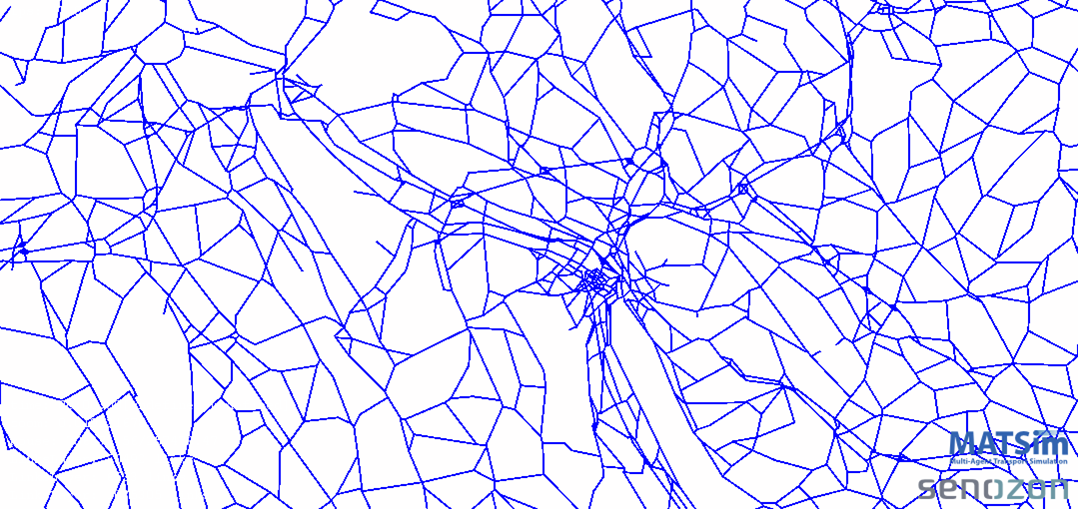
\includegraphics[width=0.8\textwidth,angle=0]{using/figures/planning.png}}%
  {\label{fig:planningnetwork}}%
  {}%
  \createsubfigure%
  {Navigation Network}%
	{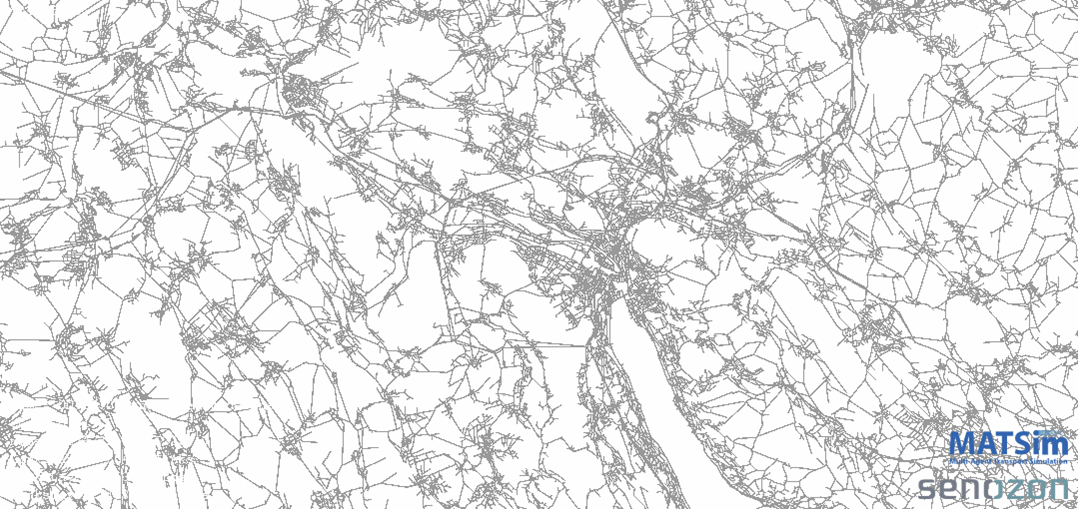
\includegraphics[width=0.8\textwidth,angle=0]{using/figures/navigation.png}}%
  {\label{fig:navigationnetwork}}%
  {}%
}%
{}

% ===============================================================================================
\subsection{Calibration, Verification, and Validation}
Calibration is a necessary task of any simulation study. Main calibration component is the utility function; it needs to reflect the preferences of the study area's population. A second prominent calibration screw is used for sample scenarios. To reduce the computational effort, initial explorative simulation runs are often performed as sample runs. In this case either the flow and storage capacity values of the mobility simulation or the network capacities need to be adapted accordingly.

Verification and validation, however, are of more concern for the microsimulation developers. Given a valuable estimate for demand and supply including a properly estimated utility function, from customer's perspective the simulation can be expected to generate valuable single run results out of the box.

The user's or customer's responsibility is asked, at another place, though. Microsimulations are basically a sampling tool, just as a survey (see Section \ref{sec:variability}). A single run represents the sampling unit, the individual in surveys. This obviously means that microsimulation results must not to be presented as single runs but with the help of the usual statistical tools, e.g., by parameters with the common measures of spread or confidence intervals. That basically means that the user/customer is responsible to specify the sample size, the number of simulation runs initialized with different random seeds. 

Policy evaluations are often based on count data, usually widely available but also showing substantial temporal variability. For MATSim, the count data need to be converted to match the simulated period of the day.

As simulation practice often mixes the terms, a few more theoretical words are said hereabout calibration, verification and validation. 

These crucial steps are located in the modeling process as sketched in Figure \ref{fig:modeling}, which is loosely based on \citet[][Figure 10.2]{Petty_SokolowskiBanks_2010}. 

\emph{Calibration} is the process of adjusting model parameters to increase consistency of model outputs and observed target values \citep[][p.348]{HollanderLiu_Transportation_2007} \citep[see also][]{TrucanoEtAl_RESS_2006}. \citet[][Table 1]{HollanderLiu_Transportation_2007} list numerous studies that each calibrate a specific transport microsimulation. Further examples are \citet[][]{SmithEtAl_JTE_2008, KimEtAl_TRR_2005, RutterEtAl_JASA_2009}, microsimulation calibration guidelines are provided by \citet[][]{MilamChao_TRBATPM_2001, WegmannEverett_TechRep_CTRUT_2008, DowlingEtAl_manual_2002}. \citet[][Table 2]{HollanderLiu_Transportation_2007} describe measures of goodness-of-fit, that are productive for calibration. Due to the usually large number of model parameters, an automated process is favorable as far as possible. Essentially this is an optimization process \citep[][p.353]{HollanderLiu_Transportation_2007}, for which various established procedures exist \citep[e.g.,][p.41ff]{ZhangMa_ResRep_PATH_2008}. For MATSim, an automatic procedure adapting the plans to road counts was developed by \citet[][]{FloetteroedEtAl_TechRep_TRANSPOR_2008}. It is unclear however, if a certain loss of behavioral soundness is caused by adapting plans according to statistical matching. On the other hand, it is unclear anyway, to date, if the MATSim relaxation transitions should be given a behavioral meaning.

Verification is the procedure to test if a ``\emph{product is consistent with its specifications [...]}'' \citet[][p.330]{Petty_SokolowskiBanks_2010}. In verification, a perfect match can be achieved comparing the conceptual and the executable model (see Figure \ref{fig:modeling}) in contrast to validation, where the model is always an approximation to reality \citep[][p.145]{Kleijnen_EJOR_1995}. According to \citet[][p.331]{Petty_SokolowskiBanks_2010}, ``\emph{validation is the process of determining the degree to which the model is an accurate representation of the simuland.}'' Validation is difficult to standardize due to the variety of models and model purposes. Some measures, tests, and applications relevant to transport modeling are given by \citet[][Table 2]{MilamChao_TRBATPM_2001}, \citet[][]{Lima_TechRep_LMPO_2006}, \citet[][p.155]{KurthEtAl_TRBTDF_2006}, \citet[][p.157]{PendyalaBhat_TRBTDF_2006}, \citet[][p.8]{WegmannEverett_TechRep_CTRUT_2008}, \citet[][]{MilamChao_TRBATPM_2001, RoordaEtAl_TransResA_2008, HawasHameed_TPT_2009, SadekEtAl_TRR_2003, GouliasKitamura_TRR_1992}, \citet[][p.25]{CambridgeSystematics_manual_2008}, \citet[][p.145]{Kleijnen_EJOR_1995} (see also \citet[][]{David_EACSSS_2009}, \citet[][p.56]{SbaytiRoden_ResRep_AASHTO_2010}, \citet[][]{SchifferRossi_TRB_2009}). While for the 4-step procedure some validation standards have emerged \citep[e.g.,][]{BartonAschmanCambridgeSystematics_manual_1997}, a lack of standardization exists for activity-based models. \citet[][]{PendyalaBhat_TRBTDF_2006} say that ``\emph{despite the appeal of these models,}'' [activity- and tour-based travel demand modeling systems] \emph{``their widespread implementation appears to be hindered by the absence of a detailed validation and assessment of this new wave of model systems. Many MPOs will not adopt such models until they are tested.}'' \citet[][]{KurthEtAl_TRBTDF_2006} cites a statement made by Chandra Bhat and Frank Koppelman in a DRCOG e-mail discussion: ``\emph{Researchers and practitioners have not thought carefully enough about the criteria for validation of models. Researchers have the habit of asking practitioners to believe that activity- based methods will produce better impact assessment and forecasts because such models more appropriately represent the actual decision process (we plead guilty to this charge). There is a good basis for this line of thought, but researchers need to go beyond this argument. They need to develop clear validation criteria and demonstrate the value of activity-based methods in ways that are easily understood.}''

Often neglected, but important, is performing sensitivity analysis (sometimes dubbed ``what-if analysis'' \citep[][p.155]{Kleijnen_EJOR_1995}) \citep[][]{KurthEtAl_TRBTDF_2006, CambridgeSystematics_manual_2008, CFD_TRB_2007}. Sensitivity analysis is similar to assessing elasticity of a variable \citep[][p.3f]{WegmannEverett_TechRep_CTRUT_2008} and it tests reaction of the model to changed parameters including model input. This includes both testing the range of parameters for a given point in time, and analysis of the system's fore- and backcasting abilities \citep[e.g.,][p.56]{CFD_TRB_2007}, \citep[][]{CambridgeSystematics_manual_2008}. As forecasting is a vital objective of most transport models, this test is crucial. \citet[][p.158]{PendyalaBhat_TRBTDF_2006} puts it succinctly: ``\emph{There is no doubt that any model can be adjusted, refined, tweaked, and---if all else fails---hammered to replicate base-year conditions.}'' and concludes that ``\emph{the quality of a travel demand model system is better judged on its ability to respond to a range of scenarios and policies of interest.}'' In MATSim, a natural and interesting sensitivity test would be to compare the MATSim forecasts with the current actual state of Zurich network after addition of the bypass ``Westumfahrung'' in 2009 \citep[][]{BalmerEtAl_ResRep_bdktzrh_2009, Westumfahrung_Webpage_2008}.

As mentioned above, models are in general flexible enough to be calibrated to target data. Thus, validation \emph{must} be performed using a different data set than for preceding modeling steps \citep[][p.1]{CambridgeSystematics_manual_2008}, \citep[][p.56]{CFD_TRB_2007}, \citep[][p.18]{OrtuzarWillumsen_2001}. In statistics, this is called cross-validation. It is particularly important for forecasting models, which need to be general enough to capture temporal changes. Calibration and validation should thus be strictly separated, however, in microsimulation practice, according to the author's opinion, they are (too) often mixed, sometimes due to the vast amount of data required for model implementation and calibration. In MATSim, for example, after model calibration only road count data is left for validation \citep[][]{HorniEtAl_STRC_2009}. New data sources, such as road speed analyses based on GPS \citep[][]{HackneyEtAl_JGS_2007}, should be included.

Having said that, validation of a large-scale transport simulation is very difficult. Many central and comfortable characteristics of systems known from natural sciences are only seldom available for the social science, such as path-independence, decomposability, isolation, and on top of that repeatability of experiments. As a result, there is still a debate if social science actually can provide something similar as laws. \citet[][p.107ff]{Abel_1976} lists and discusses the 12 claims of the ``\emph{Verstehen Position}''; although, he finds contrary arguments to every claim, nevertheless, something definitely remains true, making social science model validation exceptionally difficult. For microsimulation results interpretation and model validation, it helped me to visualize the following example. A microsimulation forecast (or backcast) regarding the construction of the ``Westumfahrung Zürich'' provides a probability distribution of scenarios, and it is essentially an exercise in Monte Carlo sampling. 4 years later we have exactly one actual state, and there is no way to assess the forecasted (or backcasted) probability distribution beyond checking that this actual state is contained in the probability distribution, and hopefully with high probability. There is nothing like Monte Carlo sampling when it comes to aggregate real system states. In other words the existing state is \emph{unique}. In essence, we thus compare an observed Dirac impulse with a computed probability distribution, which is a difficult undertaking.

% ----------
\createfigure%
{Modeling Process}%
{Modeling Process: Modeling starts with observation and measurement of reality (in \citet[][]{Petty_SokolowskiBanks_2010} called ``\emph{simuland}'') for acquisition of knowledge (in \citet[][]{Petty_SokolowskiBanks_2010} called ``\emph{referent}''). Model creation---in a strict sense usually referred to as \emph{modeling}--- is based on the modeler's knowledge about the world. Based on a conceptual model, an executable model is implemented and calibrated. The executable model is evaluated in a verification step in terms of ``\emph{was the model made right?}'' \citep[][p.332]{Petty_SokolowskiBanks_2010}. Validation compares results with the referent in the sense of ``\emph{was the right model made?}'' \citep[][p.332]{Petty_SokolowskiBanks_2010}.}%
{\label{fig:modeling}}%
{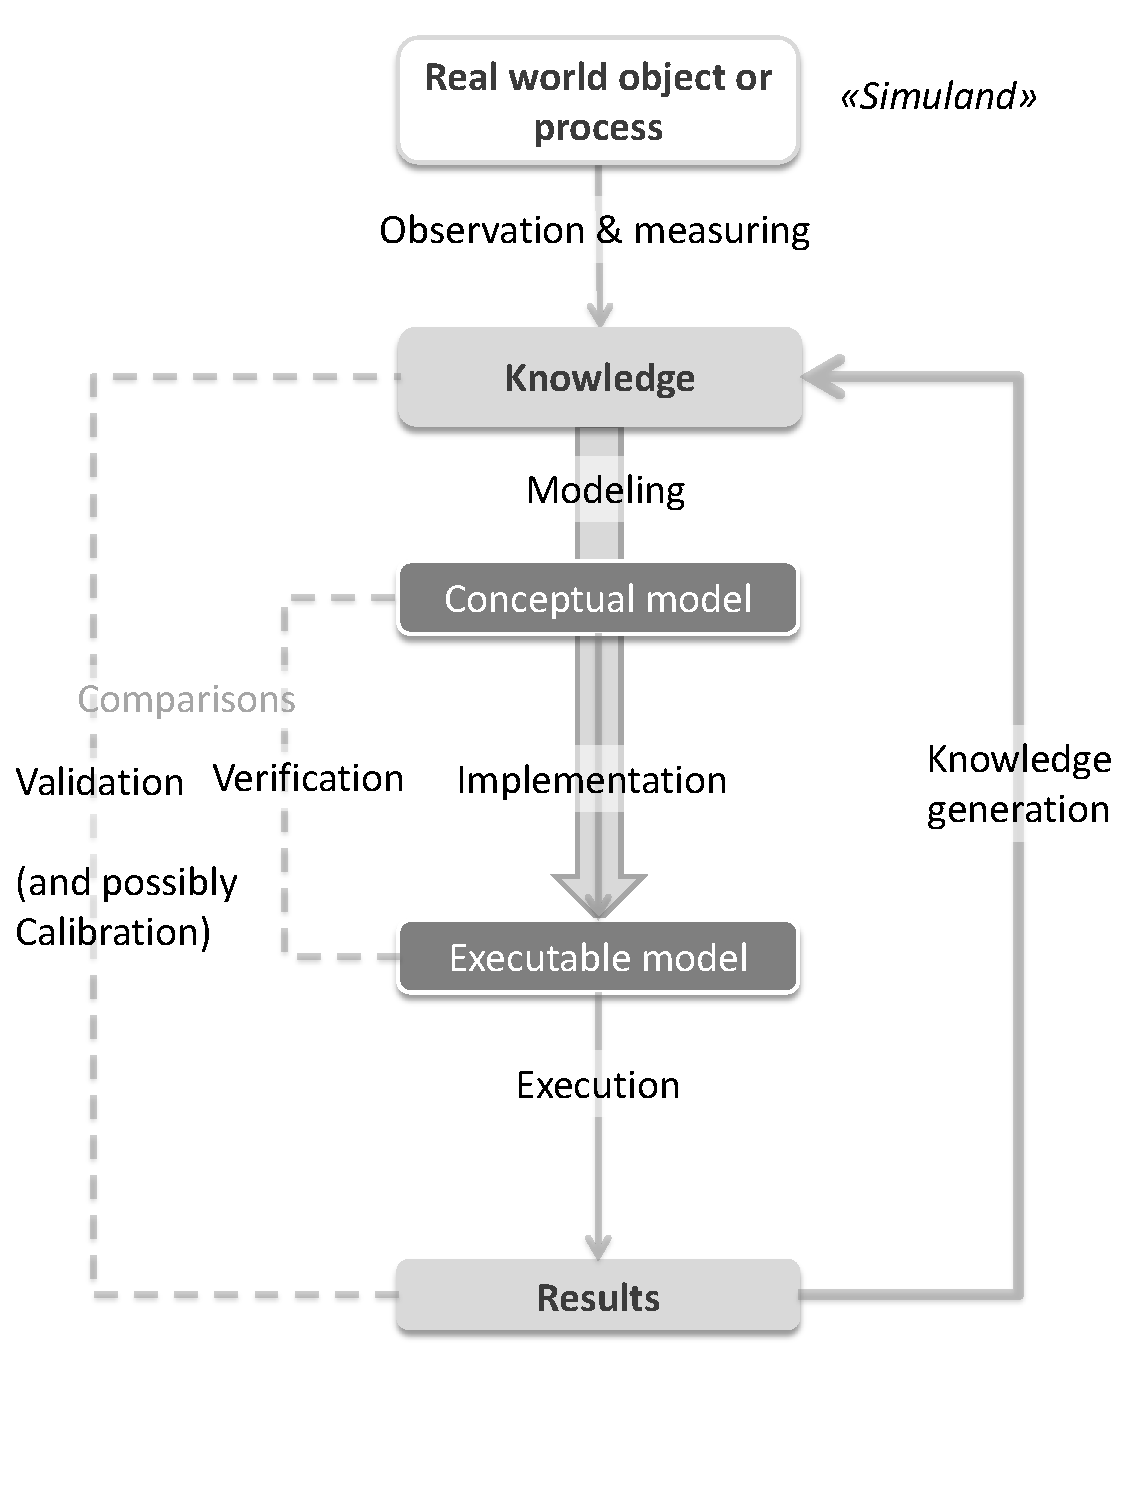
\includegraphics[width=0.8\textwidth, angle=0]{using/figures/modeling.pdf}}%
{}
% ----------

% ##################################################################################################################

% Local Variables:
% mode: latex
% mode: reftex
% mode: visual-line
% TeX-master: "../main"
% comment-padding: 1
% fill-column: 9999
% End: 
 \cleardoublepage
\chapter{A Closer Look at Scoring}
\label{ch:scoring}
% ##################################################################################################################

\hfill \textbf{Author:} Andreas Horni

\begin{center} 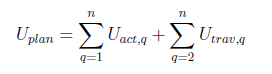
\includegraphics[width=0.3\textwidth, angle=0]{figures/scoring.png} \end{center}

% ##################################################################################################################
MATSim scoring is a central element of MATSim, nevertheless; the user can plug in any custom scoring function. 

MATSim is based on utility-maximization. Thus, estimated discrete choice models can be applied in MATSim. However, due to MATSim's iterative structure and because it is based on complete day plans, the application of models for parts of day plans only (for example mode choice) is not straight forward as detailed in Section \ref{sec:estimation}.

Due to the absence of a complete-day-utility function, MATSim has been started with the so-called Charypar-Nagel utility function (Section \ref{sec:charyparnagel}) and extended for some purposes (Section \ref{sec:utfextensions}). An readily applicable estimation for a full-day utility function is not yet available. 

% ##################################################################################################################
\section{Basic Charypar-Nagel Utility Function}
\label{sec:charyparnagel}
The first and still basic MATSim utility function was formulated by \citet[][]{CharyparNagel_Transportation_2005} from the \emph{Vickrey} model for road congestion as described in \citet[][]{Vickrey_TAER_1969} and \citet[][]{ArnottEtAl_TAER_1993}. Originally, this formulation was established for departure time choice. However, all studies performed so far, indicated that the MATSim function is also appropriate for modeling the further choice dimensions. 

For the basic function, the utility of a plan $U_{plan}$ is computed as the sum of all activity utilities $U_{act,q}$ plus the sum of all travel (dis)utilities $U_{trav,q}$:
%
\begin{equation}
\label{eq:matsimUTF}
U_{plan}=\sum^n_{q=1} U_{act,q} + \sum^n_{q=2} U_{trav,q}
\end{equation}
The utility of an activity $q$ is defined as follows (see also \citet[][p.377ff]{CharyparNagel_Transportation_2005}):
\begin{equation*}
U_{act,q} = U_{dur,q} + U_{wait,q} + U_{late.ar,q} + U_{early.dp, q} + U_{short.dur, q},
\end{equation*}
where:
\begin{itemize}
\item $U_{dur,q}= \beta_{dur,q} \cdot t_{typ,q} \cdot \ln(t_{dur,q}/t_{0,q})$ is the utility of performing activity $q$, where opening times of activity locations are taken into account. $t_{dur,q}$ is performed activity duration, $\beta_{dur,q}$ is marginal utility of activity duration for its typical duration $t_{typ,q}$ and $t_{0,q}$ is minimal duration, or in other words, the duration for which utility starts to be positive. 

\item $ U_{wait,q} = \beta_{wait, q} \cdot t_{wait,q}$ 

denotes the waiting time spent for example in front of a yet closet store, where $\beta_{wait,q}$ is marginal utility of waiting and $t_{wait,q}$ is the waiting time.
		
\item $U_{late.ar,q}= \left\{
  \begin{array}{l l}
    \beta_{late.ar,q} \cdot (t_{start,q} - t_{latest.ar,q}) & \quad \text{if $t_{start,q} > t_{latest.ar,q}$}\\
    0 & \quad \text{else}
  \end{array} \right.$
  
  specifies the late arrival penalty, where $t_{start,q}$ is the starting time of activity $q$ and $t_{latest.ar}$ is the latest possible starting time of that activity for example given by opening times.

\item $U_{early.dp} = \left\{
  \begin{array}{l l}
    \beta_{early.dp,q} \cdot (t_{earliest.dp, q} - t_{end,q}) & \quad \text{if $t_{end,q} > t_{earliest.dp,q}$}\\
    0 & \quad \text{else}
  \end{array} \right.$

defines the penalty for staying not long enough, where $t_{end,q}$ is the ending time of the activity and $t_{earliest.dp,q}$ is the earliest possible end time for activity $q$.

\item $ U_{short.dur, q} = \left\{
  \begin{array}{l l}
    \beta_{short.dur,q} \cdot (t_{short.dur, q} - t_{dur,q}) & \quad \text{if $t_{dur,q} < t_{short.dur,q}$}\\
    0 & \quad \text{else}
  \end{array} \right.$
  
  is the penalty for a too short activity, where $t_{short.dur}$ is the shortest possible duration for the activity.
\end{itemize}


Travel disutility is given as 
\begin{equation}
\label{eq:tdisutility}
U_{trav, q} = \beta_{trav, q} \cdot t_{trav, q} \,
\end{equation} 
where:
\begin{itemize} 
\item $\beta_{trav, q}$ is the marginal utility of travel by mode (normally negative or zero), and
\item $t_{trav, q}$ gives the travel time between location of activity $q-1$ and $q$
\end{itemize}

Note that the distance contributes to disutility in two ways. First, it is included in a direct manner via $\beta_{d, mode,q}$, which is natural for modes with physical efforts such as walking or cycling. Second, distance is also included moneteraily via $\beta_m \cdot \gamma_{d, mode}$ which is natural for mode car or pt, where monetary costs increase dependent on distance.

Further note that travel receives an additional implicit penalty from the opportunity cost of time: If a travel time could be reduced by $\Delta t_{trav}$, the person would not only gain from avoiding $\beta_{trav}~\cdot~\Delta t_{trav}$, but also from making activities longer. The marginal utility of travel time savings is thus:
%
\[
mUTTS = - \frac{\partial}{\partial t_{trav}} U_{trav} + \frac{\partial}{\partial t_{dur}}U_{dur} 
\]
which is 
\[
mUTTS = - \frac{\partial}{\partial t_{trav}} U_{trav} +  \beta_{dur} \cdot \frac{t_{typ,q}}{t_{dur,q}} 
\]
and at the typical duration of an activity
\[
mUTTS = \beta_{trav} + \beta_{dur}.
\]
The marginal utility of travel time savings at the typical duration can be transformed to the more common value of travel time savings by division with $\beta_{m}$:
\[
VTTS = \frac{mUTTS}{\beta_{m}} = \frac{\beta_{trav} - \beta_{dur}}{\beta{m}}
\]
This is important for calibration of the utility function.

\ah{Bildchen von Score-Entwicklung machen}

% ======================================================================================================================
\subsection{Parameters}
\label{sec:paramset}
The basic Charypar-Nagel scoring function is inspired by \citet[][]{ArnottEtAl_TAER_1993}, which provides an extension of the Vickrey model \citep[][]{Vickrey_TAER_1969}.  

\citet[][p.164, p.173]{ArnottEtAl_TAER_1993} defines 
$\alpha=5.00\ \$/h$ the shadow cost of travel time,
$\beta=3.05\ \$/h$ the unit cost of arriving early at work, and
$\gamma=11.88\ \$/h$ the unit cost of arriving late based on the estimations reported by \citet[][Table 2 on p.473]{Small_AER_1982}.
Derived from this initial values \citet[][p.382]{CharyparNagel_Transportation_2005} define the MATSim utility function as follows, where they consider the opportunity costs of $20\ EUR/h$, i.e., the costs for doing nothing. \ah{wie genau kam man auf die Werte? \\ In \citet[][p.122]{ArnottEtAl_JUE_1990}, they are defined as $\alpha=6.40\ \$/h$, $\beta=3.90\ \$/h$ and $\gamma=15.21\ \$/h$.

Bernhard and Axhausen: Metaanalysis. Normwerk. Verl�sslichkeit ...
% Chaumet, R., P. Locher, F. Bruns, D. Imhof, M. Bernard and K.W. Axhausen (2007) Verfahren zur Ber�cksichtigung der Zuverl�ssigkeit in Evaluationen, final report for VSS 2002/002, Schriftenreihe, 1176, Bundesamt f�r Strassen, UVEK, Bern. 

}
\begin{itemize}
\item $\beta_{dur,q}= 6\ EUR/h$,
\item $\beta_{trav, mode, q}= -6\ EUR/h$,
\item $U_{wait,q}=0\ EUR/h$,
\item $\beta_{late.ar,q}=-18\ EUR/h$,
\item $\beta_{early.dp,q}=-18\ EUR/h$.
\end{itemize}

\ah{$\beta_{short.dur,q}$ is not defined on page 393.}

Extensions to this basic and default utility function are described in the next section. 

% ##################################################################################################################
\section{Extensions and Estimations}
\label{sec:utfextensions}
The following paragraphs describe, how the basic utility function (Equation \ref{eq:tdisutility}) explained in \citet[][]{CharyparNagel_Transportation_2005} has been extended by monetary and distance costs and mode-specific travel parameters including constants. Please be aware, that the MATSim code base and in particular the scoring functionality has changed a lot in recent years, e.g., the scoring is now based on events rather than on plans \ah{Revision angeben!}. Thus, the historical development is accompanied by various conceptual and technical modifications leading to the current utility function described in Section \ref{sec:currentUTF}. This also means, that the reported parameter settings are an indication not a direct recommendation. Also note, that nowadays the utility function does not use monetary units anymore but it is measured in ``utils''.

\ah{Sections sind zu heterogen! \\
Generelle Struktur einbringen (template): \\
- Scenario \\
- UTF und Params\\
- Main simulation results \\
}

% ======================================================================================================================
\paragraph{Calibration Project Westumfahrung Z�rich:}
Project Westumfahrung \citep[][]{BalmerEtAl_ResRep_bdktzrh_2009} used the Z�rich scenario version 1 \citep[][]{HorniEtAl_TechRep_IVT_2011_a}. Only car traffic was simulated with $\beta_{perf,q}=6.0\ utils/h$ and $\beta_{trav,q}=-6.0\  utils/h$. No further penalties were applied. Typical activity durations were provided with the config with half-hour resolution and empirically founded on the Swiss microcensus.

% ======================================================================================================================
\paragraph{Estimation Kickh�fer:}
\citet[][]{Kickhoefer_MastersThesis_2009} added monetary variables and income to the MATSim utility function and performed a mode-specific estimation based on the survey by \citet[][]{VrticEtAl_ResRep_SVI_2007}. The utility function extended by monetary factors was linear, both in the variables and the parameters. Estimated parameters are given in Table 3 of \citet[][]{Kickhoefer_MastersThesis_2009}. The income-dependent utility function was based on \citet[][]{Franklin_PhDThesis_2006}.

% ======================================================================================================================
\paragraph{Calibration Project Location-Based Services:}
\citet[][]{BalmerEtAl_ResRep_datapuls_2010} was simulated on the Swiss scenario version 2 \citep[][]{HorniEtAl_TechRep_IVT_2011_a}. Innovations related to the utility function are agent-specific typical activity durations and facility-specific opening hours. Summation of activity duration for activities of the same duration (denoted as $U_{cum}$) was invented \citet[][p.9 and p.28]{BalmerEtAl_ResRep_datapuls_2010}. To prevent agents to invest all the time in a single activity a very high penalty for too short activities ($U_{short,q} = -180\ utils/h$) was applied. Facility-load as detailed below was included. The parameters \citep[][Table 2 on p.31]{BalmerEtAl_ResRep_datapuls_2010} of the multi-modal utility function including monetary costs was heavily based on the estimation of Kickh�fer \citep[][]{Kickhoefer_MastersThesis_2009}. Egress and access times to and from public transport stops was included, where public transport travel times were not simulated but estimated. Due to problems with spreading of many plans into the next day a penalty for too long day plans was applied.

% ======================================================================================================================
\paragraph{S-Shaped Function and Its Estimation:}
Both \citet[][p.127f]{Feil_PhDThesis_2010} and \citet[][p.32]{MATSim_Userguide_2014} report that the standard logarithmic function of MATSim is not suitable for modeling activity choice. Due to the log form very short activities are favored, which means that the schedule is filled-up with numerous quick activities, where the usually long home activities are replaced first. Since this is unrealistic behavior, a new function was introduced by \citet[][p.129ff]{Feil_PhDThesis_2010}. The function is based on \citet[][]{Joh_PhDThesis_2004} and is asymmetrically S-shaped. First estimations of the new function based on the Swiss microcensus were provided, which were calibrated for the schedule recycling functionality \citet[][p.152f]{Feil_PhDThesis_2010}. The function was not developed further.

% ======================================================================================================================
\paragraph{Calibration Project Herbie Mode Choice:}
Project Herbie \citep[][]{VitinsEtAl_VW_2012} provided a thorough calibration of the multi-modal Z�rich scenario extended by public transport simulation, cross-border and freight traffic, tolling, parking pricing, park \& ride and joint riding. The mode-share calibration targeting on distances and shares was based on the Swiss microcensus \citep[][p.18]{VitinsEtAl_VW_2012}.   

% ======================================================================================================================
\paragraph{Calibration Project Tel-Aviv:}
\citet[][]{BekhorEtAl_TRB_2011} combines MATSim with the Tel-Aviv activity-based model \citep[][]{CambrigeSystemsInc_ResRep_TelAviv_2008}. Its multi-nomial zone-based utility function is integrated into MATSim by disaggregating the zones into facilities. \ah{add working paper about Tel Aviv destination choice.}

% ======================================================================================================================
\paragraph{Calibration Project MATSim 2030:}
Switzerland. \ah{wait for working paper}

% ======================================================================================================================
\paragraph{Calibration Singapore Scenario:}
In the Singapore scenario \citep[][]{ErathEtAl_IATBR_2012} the basic multi-modal Charypar-Nagel utility function is applied. Its parameters derived from the Singapore Land Transport Authority (LTA) model. The utility function is measured in SGD rather than utils.

% ======================================================================================================================
\paragraph{Car Sharing Scoring:}
\citet[][p.10]{CiariEtAl_TechRep_IVT_2014} used the following car sharing specific utility function terms: access and egress time costs for walking, monetary cost of distance, and rental costs (constant and time-dependent). Simulations were performed for the multi-modal Z�rich scenario with the parameter set described in Table 1.

% ======================================================================================================================
\paragraph{Parking Scoring:}
\citet[][]{WaraichAxhausen_TechRep_IVT_2012} extended the utility function by a parking term including walking to and from the parking lot (p.7) and parking costs (p.9). Simulations were run for the Z�rich car traffic scenario. \citet{WaraichEtAl_unpub_TRB_2013} implemented an estimated parking location choice model provided by \citet[][]{WeisEtAl_TechRep_TSMS_2013}.

% ======================================================================================================================
\paragraph{Road Pricing Scoring:}
Road pricing is a MATSim extension. It can be added by an event listener to the controler. The utility function then gets money events and accumulates it to the rest of the score.

% ======================================================================================================================
\paragraph{Social Contacts and Joint Trips Scoring:}
There are two approaches modeling social contacts in MATSim, namely \citet[][]{Hackney_PhDThesis_2009} and the work performed Thibaud Dubernet. Both modify scoring in a similar way; by increasing each individuals score if they coincidently perform an activity of the same type in the same facility. Both restricted the type to leisure to begin with. Dubernet also includes joint car rides in that calculation; but sometimes instead the marginal utility of travel is modified (Thubaud Dubernet, personal communication, March 2014). Linear and logarithmic functions have been tried by Dubernet, where recent experiments showed that, as expected, a logarithmic function increases the number of friend contacts, giving the microsimulation user another calibration screw at hand. 

% ======================================================================================================================
\paragraph{Facility Load Scoring:}
The influence of interaction in \emph{transport} infrastructure for people's route and departure time choice has been recognized early \citep[e.\,g.,][]{Pigou_1920, Knight_QJE_1924, Wardrop_PICE_1952}. Similarly, it can be reasonably assumed that agent interaction in \emph{activities} infrastructure affects travel choices \citep[][]{Axhausen_SSRL_2006}. Marketing science provides ample evidence that agent interactions influence utility of performing an activity, where it can have both, positive or negative influence \citep[][p.331]{BakerJEtAl_JAMS_1994}, \citep[][]{ErogluAndHarrell_JR_1986, ErogluAndMachleit_JR_1990, ErogluEtAl_JBR_2005, HarrellEtAl_JMR_1980, HuiAndBateson_JCR_1991, PonsEtAl_PsychMark_2006}.

In \citet[][]{HorniEtAl_TRR_2009}, based on the Z�rich scenario, a singly-constrained model is presented that introduces competition for space-time slots on the activity infrastructure. The actual load is coupled with time-dependent capacity restraints for every activity location and incorporated explicitly into the agent's destination choice process as detailed below. 

Activity location load, computed for time bins of 15 minutes, is derived from events that are delivered by the Mobsim. The load of one particular iteration combined with time-dependent activity location capacity restraints is considered in the agents' choice process of the succeeding iteration. In detail, this means that the utility function term $U_{dur,q}$, described above, is multiplied by $max(0; 1 - f_{load\ penalty})$ penalizing the agents dependent on the load of the location they frequented. $f_{load\ penalty}$ is a power function, as this has shown to be a good choice for modeling capacity restraints (remember that the well-known cost-flow function by \citet[][]{TA_manual_1964} is a power function). To introduce additional heterogeneity regarding the activity locations, an attractiveness factor $f_{attractiveness}$ is introduced that is defined to be logarithmically dependent on the store size given by the official census of workplaces.

Likewise for demonstration purposes, capacity restraints are exclusively applied to shopping locations, where in principle leisure activity locations could be handled similarly. However, deriving capacity restraints for leisure activity locations is expected to be much more difficult than for shopping locations because data availability is much smaller for leisure locations and capacity restraints vary much more between different leisure locations than between different shopping activities (hiking versus going to the movies might be an illustrative example).

The model allows the assignment of individual time-dependent capacities to the activity locations. For the sake of demonstration, the capacities of all shopping facilities are set equal, where the values are derived from the shopping trip information given in the National Travel Survey of 2005. The total daily capacity is set so that the activity locations located in the region of Zurich satisfy the total daily demand with a reserve of 50\%. In detail, the capacity restraint function for a location $i$ is as follows:

\[
f_{load\ penalty, i}=\alpha_i \cdot \Bigg(\frac{load_{i}}{capacity_{i}}\Bigg)^{\beta_i}
\]
with $\alpha_i=1/1.5^{\beta_i}$, $\beta_i=5$. $f_{load\ penalty, i}$ is the penalty factor for location $i$ as described above.

The simultaneous computation of the score reduction for all agents avoids the last-record problem discussed in \citet[][]{VovshaEtAl_TRR_2002}. Therein, a sequential choice process is proposed where alternatives are removed from the choice set of the later travelers if the locations are already occupied by the earlier travelers. Thereby, the order of the travelers is specified arbitrarily and thus the last-record problem (the last travelers have to travel far to find an available location) is not negligible when modeling heterogeneous travelers. 

As expected, the constrained model improves results' quality by reducing the number of implausibly overcrowded activity locations.

% ======================================================================================================================
\paragraph{Error Terms:}
MATSim as a utility-maximizing model is strongly related to the discrete choice framework, meaning that this framework might guide the MATSim utility function specification. Utility in discrete choice models is composed of a deterministic part and a random error term. The random error term represents the unobserved heterogeneity, i.e., it subsumes, both, truly, i.e., inherently random decisions and the modeler's missing knowledge about the choice and its context. 

In MATSim, the utility function for route, mode and time choice does not contain a random error term (yet). This can be regarded as a shortcoming of the model. However, this is at least partially compensated through the stochasticity of the replanning. First, route and time choices are usually subject to significant competition. The co-evolutionary algorithm of MATSim, detailed below, essentially assigns the resources in a random manner to the persons. For example, two identical persons may end up with different routes according to the order in which they undergo the replanning. Essentially, this means that a random term is present in the choice modeling. However, this randomness is introduced implicitly and not in a systematic manner. In other words, choice outcomes do not only depend on implemented choice model, but are also implicitly influenced by the implementation of the algorithm to find the solutions of the utility-maximization. This is difficult to interpret, and, furthermore, replanning did up to now not add enough unobserved heterogeneity to destination choice. Thus, an explicit random error term $\epsilon_{piq}$ for every person $p$, alternative $i$ and activity $q$, held stable over the iterations, is added to the destination choice utility function \citep[][]{Horni_PhDThesis_2013}. Research about the necessity of error terms for the remaining choice dimensions is required.

% ======================================================================================================================
\paragraph{Agent-Specific Preferences:}
In project Surprice \citet[][]{HorniEtAl_TechRep_IVT_2012_a, HorniAxhausen_TechRep_IVT_2014}, agent-specific travel preferences and individual income-dependent marginal utilities of money are incorporated. It is simulated with a 1\% multi-modal Z�rich scenario, the preference values however, are assigned randomly. 

% ======================================================================================================================
\paragraph{Estimation Destination Choice:}
Goal of the estimation described by \citet[][]{Horni_PhDThesis_2013} were first indications about quantitative relation of MATSim time parameters and further choice attributes. Focusing on destination choice, attributes used for estimation were \emph{store size} (in categories), \emph{price level} (in categories) and \emph{additional linear distance} to the store similar to the detour distance defined in \citet[][]{ArentzeTimmermans_TRR_2007}.

Clearly, for direct application in MATSim, travel times rather than distances would have been better, but this information was not available consistently. A minimal set of variables was chosen due to data availability and as the main goal was laying an instructive base for future MATSim utility function estimations and their application in the MATSim Z�rich scenario. Alternative-specific constants were not assigned to destinations to prevent over-fitting \citep[][]{BierlaireEtAl_TransScience_1997}.

Although the estimated parameters had to be enlarged to show significant effects, their relation was correct as experiments with this extended and adapted model showed a surprisingly substantial decrease of the relative error in count data.

Non-linear estimated models containing travel time are scarce as travel time is an unreliable information in surveys. A way to approximately applying simple linear distance models to the non-linear time-based MATSim utility function is discussed in Section 5.5.1 of \citet[][]{Horni_PhDThesis_2013}.

% ======================================================================================================================
\section{Current Utility Function}
\label{sec:currentUTF}
The current MATSim utility function is still the one given by Equation \ref{eq:matsimUTF}, but the travel travel scoring as now as follows.
%
\begin{equation*}
\label{eq:utfextended}
U_{trav, mode, q} = C_{mode} + \beta_{trav, mode, q} \cdot t_{trav, q} + \beta_{m} \cdot m  + (\beta_{d, mode, q} + \beta_{m} \gamma_{d, mode}) \cdot d_{trav,q} + V_{transfer,q} \,
\end{equation*} 
where:
\begin{itemize} 
\item $C_{mode}$ is a mode-specific constant,
\item $\beta_{trav, mode, q}$ is the marginal utility of travel by mode (normally negative or zero),
\item $t_{trav, q}$ gives the travel time between location of activity $q-1$ and $q$
\item $\beta_{m}$ is the marginal utility of money (normally positive),
\item $m$ are the monetary costs of the complete leg such as tolls or fares (normally negative),
\item $\beta_{d, mode}$ is the  marginal utility of distance (normally negative),
\item $\gamma_{d, mode}$ is the mode-specific distance cost rate (normally negative),
\item $d_{trav, q}$ is the distance traveled, and,
\item $V_{transfer, mode, q}$ are transfer penalties in public transport (normally negative). 
\end{itemize}

\ah{Gesamtanalyse und Vergleiche aller Beitr�ge hier angeben.}

% ##################################################################################################################
\section{Estimating a Utility Function}
\label{sec:estimation}
With the exception of \citet[][]{BalmerEtAl_ResRep_datapuls_2010}, the estimation of \citet[][]{Kickhoefer_MastersThesis_2009} has not been considered for the various calibrations and extensions mentioned above although it represents a valuable base for further estimations. Having such a base at hand is important as estimating and applying a MATSim utility function is non-trivial due to the following. 

The agents optimize complete day plans (see also \citet[][Section 6.3.1]{MATSim_Userguide_2014}). This means that the single choice dimension utility terms need to neatly fit into the complete function. It is not possible to apply functions estimated independently for only a single choice dimensions. If for example all alternatives for destination choice evaluated with an inappropriate utility function generate negative utility, then the complete activity is simply dropped. This correlation or dependency between choice dimensions is also the reason why a day plan equilibrium does not necessarily include a Nash equilibrium for every single choice dimensions (see Section \ref{}). The inseparability of choice dimensions means that in MATSim we can only consistently handle choices if we assume an absolute utility level rather than a relative level usually assumed for discrete choice models. 

Incorporating an extension, for example for parking or destination choice, in combination with absolute utilities becomes even more tricky as the Charypar-Nagel function is non-linear, which means that available models very often being linear, need to be incorporated by workarounds such as approximation procedures and distinction of cases as described in \citet[][p.75ff]{Horni_PhDThesis_2013}. Furthermore, it is based on travel times, which is usually seen as an unreliable information gathered from classical surveys. GPS or smartphone-based surveys, however, provide this information with great precision and, thus, they are advantageously used for future estimations.

Furthermore, travel time and activity duration estimations including income need to carefully consider the parameters' relation to the value of travel time savings. \citet[][p.276]{MeisterEtAl_SVT_2009} for example argues that the average Swiss hourly earnings are much higher than $6\ EUR/h$. However, the MATSim is measured in utils not monetary units anymore. But still, the parameters in utils and monetary terms (such as tolls, parking costs, fares etc., or income-dependent attributes) are often interacted and thus their relation needs to be consistent.

A numerical problem, particularly relevant for activity choice, concerns the functional form of the utility function. As argued in \citet[][p.33]{MATSim_Userguide_2014}, a function offering an additional degree of freedom (the curvature at the typical duration) would be favored.

% ##################################################################################################################
 \cleardoublepage
\chapter{Scenarios}
\label{ch:scenarios}
% ##################################################################################################################

\hfill \textbf{Authors:} (Marcel Rieser?), Andreas Horni, Benjamin Kickh�fer, Dominik Ziemke, Joschka Bischoff, ...

\begin{center} 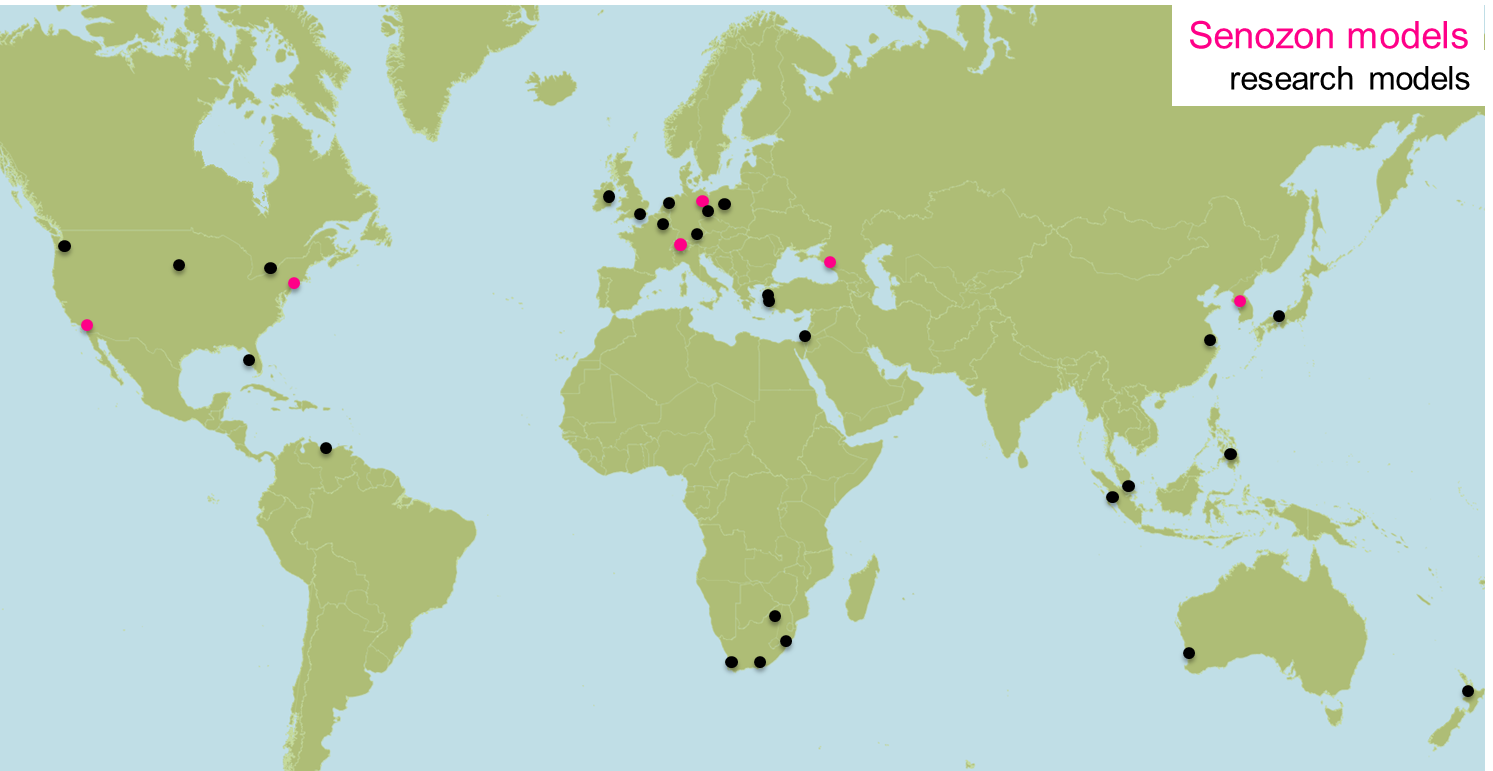
\includegraphics[width=0.7\textwidth, angle=0]{using/figures/scenarios} \end{center}

% ##################################################################################################################
This chapter summarizes available MATSim scenarios as located on the map in Figure~\ref{fig:scenarios} and summarized at \citet[][]{MATSIM-T-Scenarios_Webpage_2014}).

Many scenarios are not public due to data privacy issues. However, knowing about the general methods and approaches adopted for scenario creation and hearing about problems faced thereby might significantly support the building of new scenarios. Content basically covers information on study area, population and demand generation, activity locations, network, simulated modes, calibration and validation, achieved results, associated projects, where to find more, where emphasis is put on specialties of a certain scenario, be it parsimonious data usage procedures, special modules used, or special modes simulated (such as the parataxis in the Gauteng scenario). Some of the scenarios are used since years with a continuous further development. We target at reporting, the latest version. 

Different levels of MATSim involvement are possible. For some regions and projects, MATSim is, for example, only used for traffic assignment whereas for others the complete demand is endogenously handled. Couplings with other forecasting models for transport demand generation have been successfully applied such as the coupling with TASHA for Toronto or the combination of MATSim with the activity-based transport model of Tel Aviv.

\createfigure%
{Scenarios Overview}%
{Scenarios Overview}%
{\label{fig:scenarios}}%
{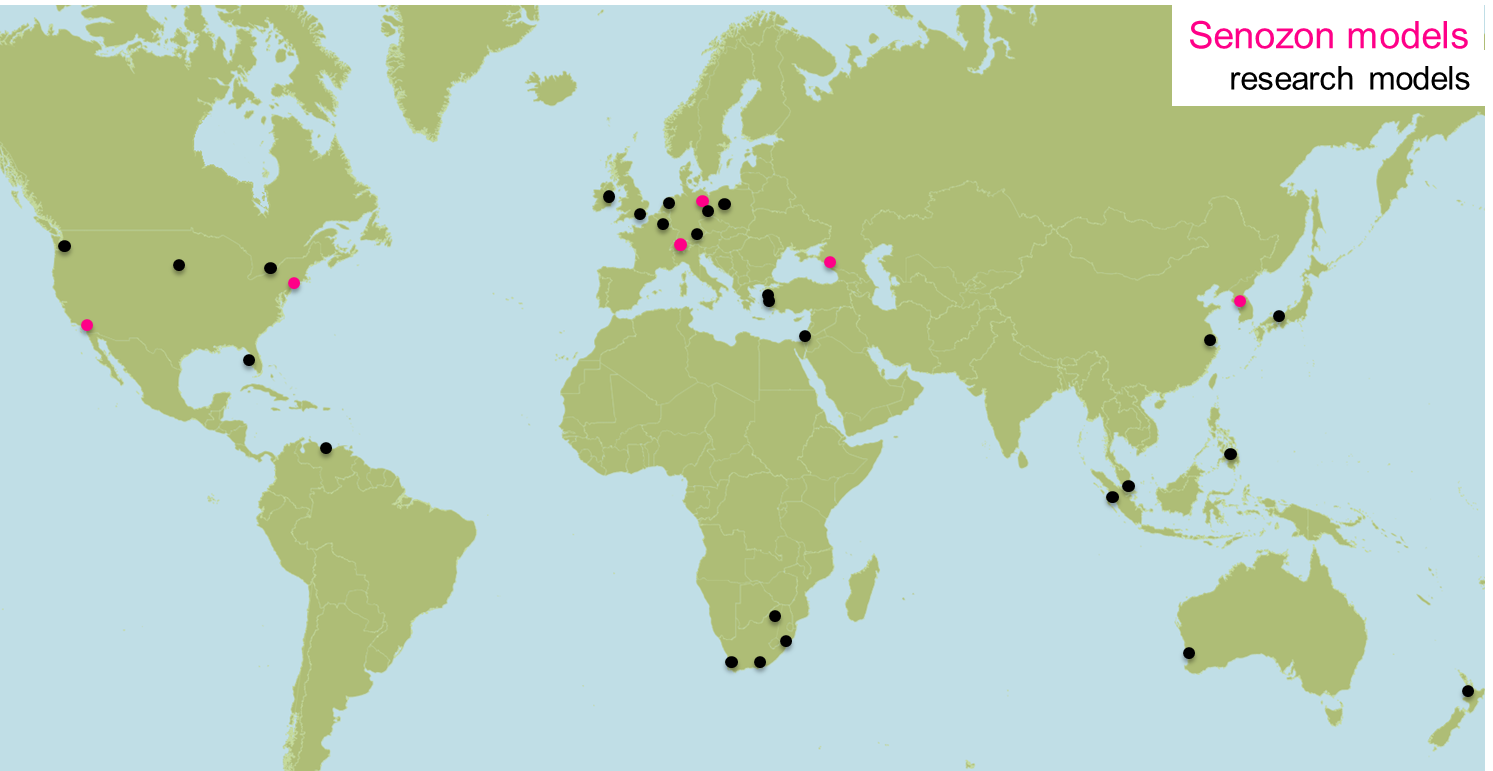
\includegraphics[width=0.99\textwidth, angle=0]{using/figures/scenarios}}%
{}

% ==================================================================================================================
% ##################################################################################################################
\section{Berlin I: BVG Scenario}
\label{sec:berlinI}
\hfill \textbf{Author:} Andreas Neumann

% ##################################################################################################################
The \gls{bvg} is Berlin's main public transport company and runs all kind of services with the exception of the S-Bahn urban rail system. This includes bus services, the subway network, the largest tram network of Germany as well as ferry services. The bus network consists of 149\,different lines, 6\,468 directed stops and a vehicle fleet of 1\,316 buses \citep{BVG2012}. In total, about 937\,million trips were served by \gls{bvg} in 2012, 41\,\% of them by bus.

% ------------
\createfigure%
{The city of Berlin and its transit network.}%
{The city of Berlin and its transit network.}%
{\label{fig:scenario_berlin_i}}%
{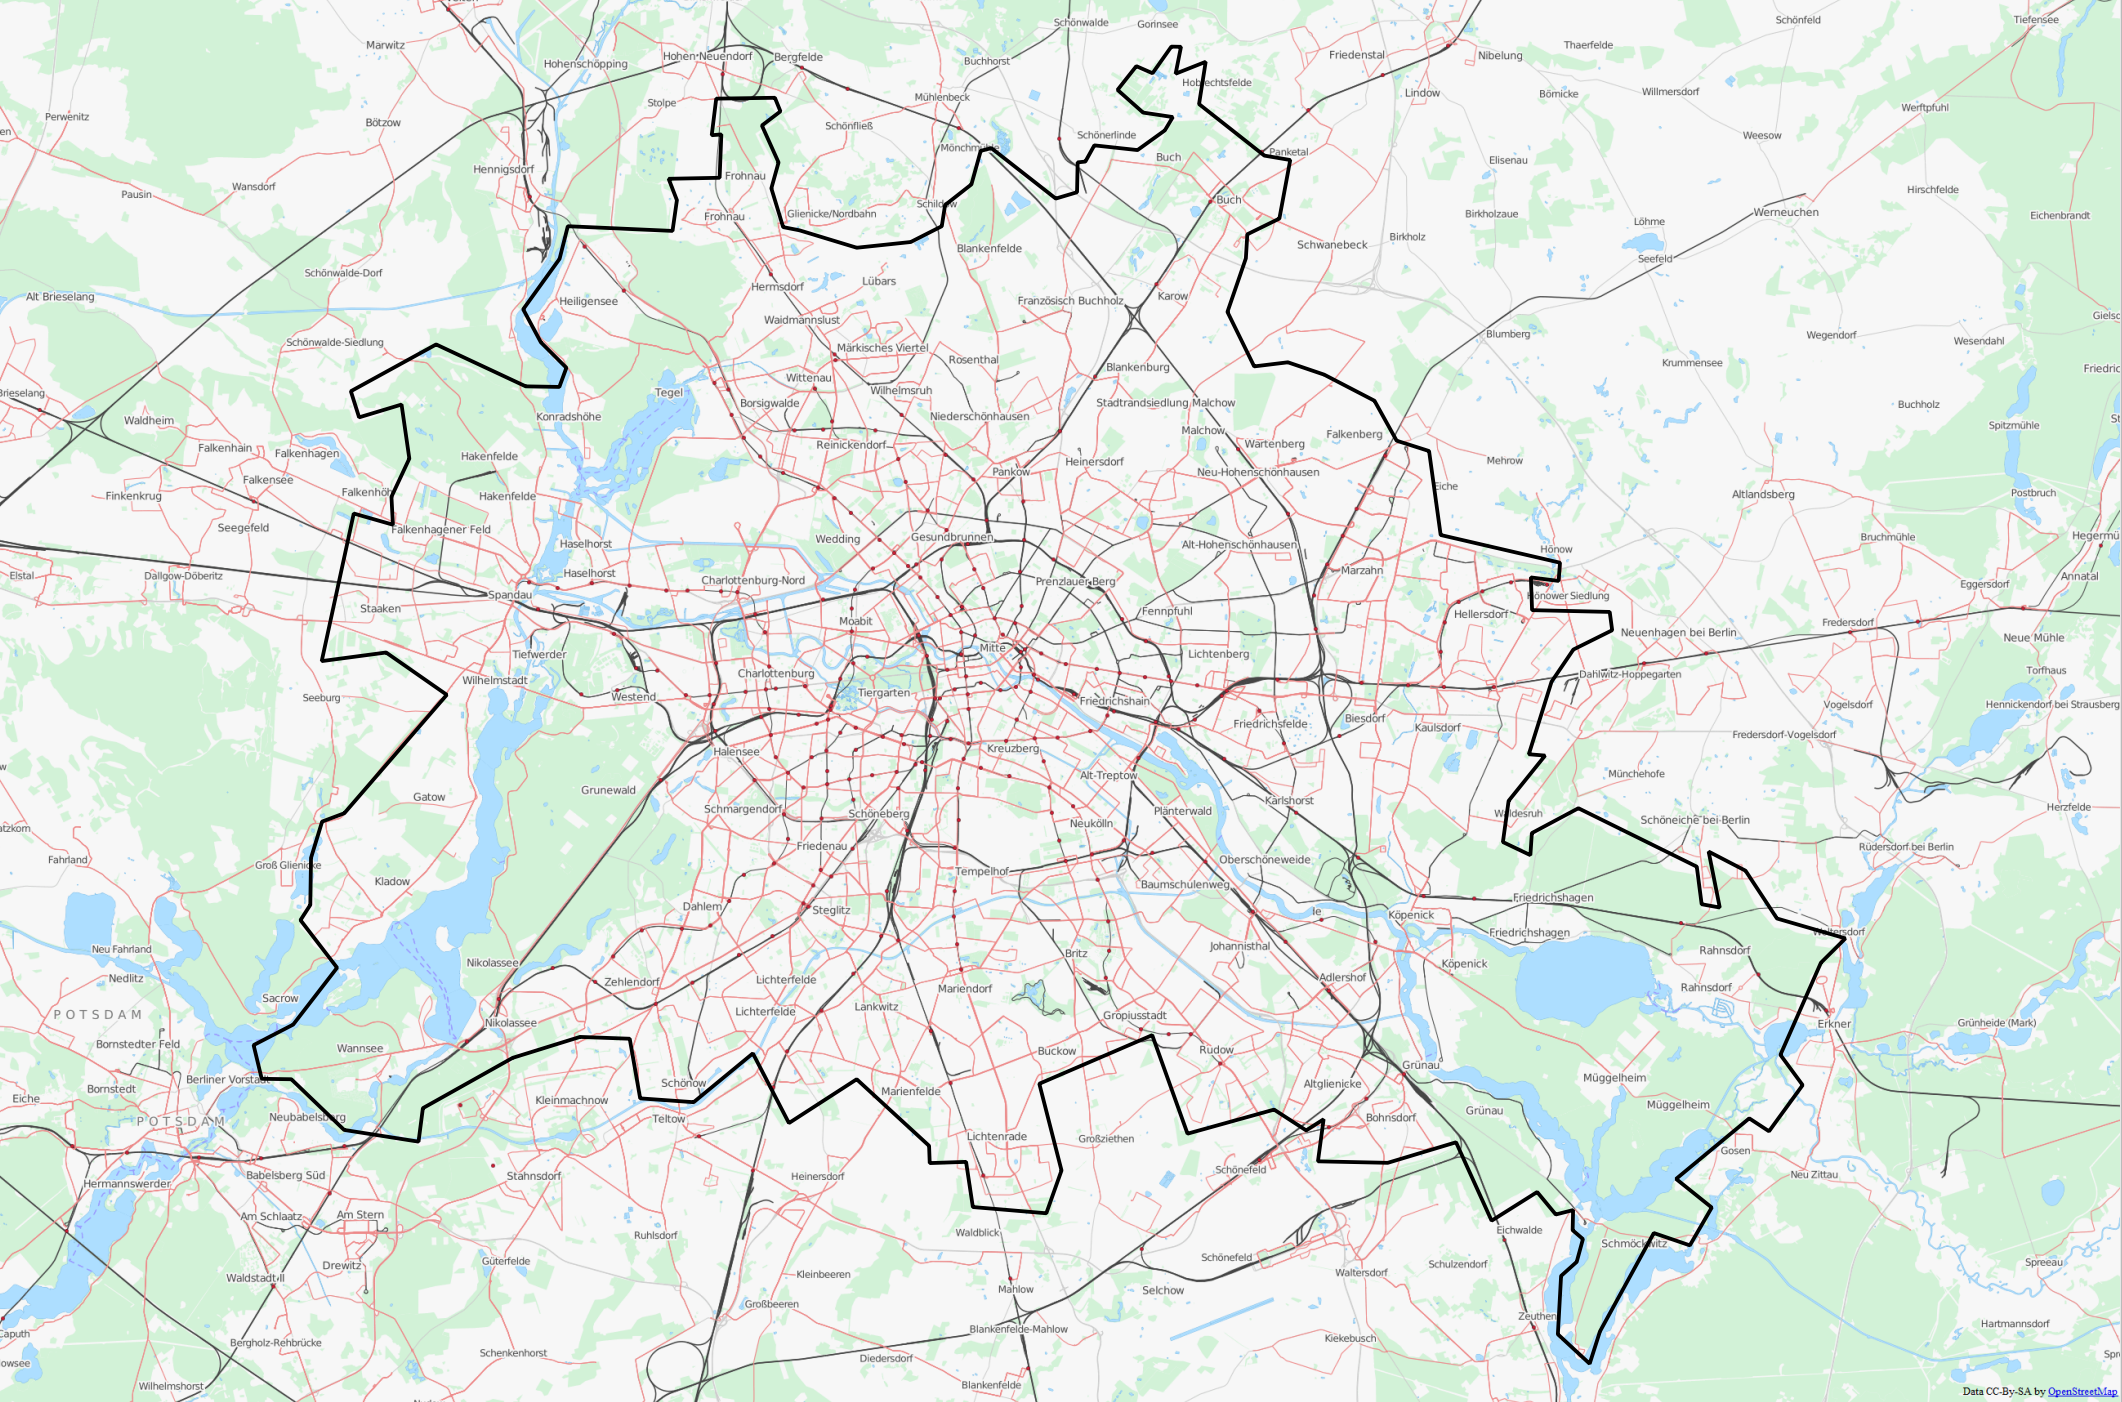
\includegraphics[width=0.99\textwidth, angle=0]{using/figures/berlin_pt}}%
{}
% ------------

% start excerpt from the paper
With the opening of the new international airport of Berlin and Brandenburg BER,
Berlin is expecting some major changes in travel demand. Especially, the
existing airport Tegel, currently exclusively served by buses operated by \gls{bvg},
will cease operations. \gls{bvg} had thus a large interest in a new transport model
for the Berlin area. Due to the big changes, the model should not only deliver
the basis for future planning of the regional transport system, but has to
provide detailed information about passenger flows of different user groups as
well. Such user group specific analyses are considered of high importance for
the \gls{bvg} in order to provide a basis for their future business strategies, which
is why an agent-based model was specifically requested. Two scenarios were
actually asked for, one for the year 2008 (actual state), and one for the year
2015 (prediction). To fulfill the needs mentioned above, the team of 
\citet{PTV2013}, \citet{Senozon2013} and \citet{VSP2013} at Technische Universität Berlin (TU Berlin)
offered a combined model consisting of both a static macroscopic model built with
\gls{visum} as well as an integrated activity-based demand and
dynamic traffic assignment model built with \gls{matsim}. During
the project, attention was given that both models were based on the same data
sources and that both modeling processes interact with each other to allow data
exchange between the two models.
% end excerpt from the paper

In brief, the model contains about 115\,000 links, % 113269
about 15\,000 directed stops, % 14902
6.0~million agents, % 4422012 (sex) 5992771 (/person)
and 539\,public transport lines operated by \gls{bvg} and other companies of the city
of Berlin and the state of Brandenburg. Among others the model features the transport 
modes Besides the transport modes car, For a more in-depth description of the
model, its generation and its calibration, the reader is referred to the work of
\cite{NeumannEtAl2014IatbrPtBerlinBook}. The model has been extensively been used in 
\citet[][Ch 7/8]{Neumann2014PhD} for the development of the minibus module of Section~\ref{sec:paratransit}.

% ################################################################################################################## ok

% ==================================================================================================================
% ##################################################################################################################
\section{Berlin II: CEMDAP-\protect\gls{matsim}-Cadyts Scenario}
\label{sec:berlinII}
\hfill \textbf{Author:} Dominik Ziemke

\editdone{This text has undergone the professional edit. Please no grammatical changes anymore! They are most-probably wrong.}

% ##################################################################################################################
%As explained in section ?????, transport modeling can be considered as the representation of the interaction of transport demand (i.e. people and goods being transported) and transport supply (i.e. transport infrastructure and services) in the transport system. Depending on the application of innovative strategy modules (see section ?????), MATSim accounts for the adaption of transport demand to transport supply \citep{Balmer2007phd}. It is, therefore, crucial to distinguish choice dimensions, which may be adapted during the modeling process (via the application of innovative strategy modules, see section....) and choice dimension whose initial properties are assumed to be correct (e.g. mode shares have to be initially correct in a scenario where the choice of transport modes is not modeled). In the latter case, it is important that respective properties of the transport demand are correct at the start of the simulation (see section Data Requirements - Demand???).
%
To correctly model initial demand properties not included in \gls{matsim} iterations in specific studies (i.e. activity choice), suitable data are needed. Travel diaries containing departure times sequences, mode choice decisions and activity locations are widely used.
%
%A disadvantage of using trip diaries is, however, that all information that is taken from the diaries is by definition not sensitive to policy measures. Also, trip diaries are normally only available for a very small fraction of the population. Another drawback is that, in Germany and the U.S. (and many other parts of the world), the geo-coding of the activity location is considered sensitive information under privacy legislation, and thus increasingly difficult to obtain (cite ZiemkeNagelBhat2015).
However, much of this data source content, particularly location information, is considered sensitive in terms of data privacy legislation and thus increasingly difficult to obtain and process in many areas (e.g.,\,in Germany and the United States) \citep{ZiemkeNagelBhat2015IntegratingCemdapMatsimTransferabilityTRB}.

The \textit{Berlin II scenario} (also referred to as the \emph{CEMDAP-\gls{matsim}-Cadyts scenario} according to applied models in its setup), is the outcome of an alternative approach relying exclusively on freely available and easy-to-obtain input data. Starting points for this scenario are publicly available commuting matrices containing homes and workplaces of workers with social security on the municipality level. Based on this information, it is possible to model morning and evening commuting peaks.

To obtain a full-population demand representation, two further major modeling steps are required. First, in cases like the Berlin case, see below, where commuter matrix spatial resolution is quite coarse, higher resolution \gls{od} information is necessary. Second, a procedure is needed to model secondary activities, i.e.,\,all other activities beyond home and work.

The importance of the first step becomes obvious when looking at the German case; here, the whole city of Berlin, with 3.4\,million inhabitants, is represented by exactly one zone \citep{BA2010Pendlerstatistik}. In the United States, commuting matrices are typically available only on a county-to-county level. Since such location-aggregation-based matrices may become the rule, rather than the exception, in privacy-sensitive societies, a (generalizable) method to attain \gls{od} information at a higher resolution is needed \citep{ZiemkeNagelBhat2015IntegratingCemdapMatsimTransferabilityTRB}. The standard solution would be to estimate an activity location choice model. This, however, is difficult if no trip data to estimate the model is available. \gls{od} matrix estimation studies \citep{ZuylenWillumsenMatrix-from-cnts} suggest that traffic counts may be used to make an initially rough \gls{od} matrix more appropriate for a region. As \gls{matsim} is not based on \gls{od} flows, but on full daily plans, the issue comes down to whether a procedure exists to update these initial full daily plans using traffic counts. In the approach used to create the Berlin II scenario, a procedure proposed by \citet{FloetteroedBierlaireNagel2010Bayesian} and implemented in the software \gls{cadyts}---explained in Chapter~\ref{ch:cadyts})---is applied for this task. Specifically, random draws of possible home and work locations within the home or work municipality given by the commuter matrix are made. Various \gls{matsim} plans, each containing one pair of home and work locations, are created for each agent. Then, the \gls{cadyts} calibration procedure is applied within the iterative \gls{matsim} simulation to select plans and locations more likely to occur with given traffic counts.

As stated above, however, full daily plans (as opposed to mere home-work-home commuting patterns) are needed. Therefore, the second modeling step, the modeling of secondary activities for each individual in the region, needs to be addressed. For the Berlin II scenario, \gls{cemdap} is used to generate initial complete daily plans for each individual. One one hand, however, no \gls{cemdap} parameter set is available for Berlin. On the other hand, and more importantly, one major goal of the study creating the Berlin II scenario was to show its generalizability \citep{ZiemkeNagelBhat2015IntegratingCemdapMatsimTransferabilityTRB}. So, the model parameters of \gls{cemdap} estimated for the Los Angeles region (the estimation context) are retained and then used to generate initial plans for individuals in Berlin (the application context in the current paper), based on Berlin demographic data.

To sum up, home and work municipalities are taken from the commuter matrix. Within these municipalities, a set of (more precisely spatially defined) potential home and work locations are randomly chosen for each agent. Full daily plans incorporating the various potential locations of each agent are generated with \gls{cemdap}, based on a parameter set from another region and local demographic data.

Then, the \gls{cadyts} calibration procedure is used to select those initial full daily plans most consistent with Berlin traffic count data. In other studies, \gls{cadyts} has already been applied to update route choice predictions, both for car \citep{FloetteroedChenEtAl2011BehavioralCalibAndAna} and for public transit \citep{MoyoNagel2013ptNetCalibrationABMTPO}. However, it has not been used to update full daily activity-travel plans, as it was in the procedure that created the Berlin II scenario. 

The Berlin II scenario is an activity-plan-based \gls{matsim} transport model for Berlin based exclusively on freely, or readily, available data. If a commuter matrix, some basic population demographics and traffic counts (or, theoretically, another suitable data source on which to run the calibration procedure) are available for a particular regional context, the approach used to create the Berlin II scenario can be transferred to this context. In fact, the Berlin II scenario itself should be seen as a \emph{transferred model}, because initial plans generated by \gls{cemdap} are based on parameter estimates from another geographic region (the Los Angeles area).

Through a validation based on the Berlin 2008 \gls{srv}, an extensive, regularly-conducted travel survey, the created transport demand representation quality has been successfully tested. So far, the Berlin II scenario exists for a 1\,\% and a 10\,\% population sample of all persons, i.e.,\,including workers without social security, as well as non-working people, aged 18 and above, for the study region. Currently, only motorized traffic is considered. Stability tests, showing that agents' daily plans continue to be chosen when \gls{cadyts} calibration functionality is switched off, have been successfully carried out. This is a clear indication that the scenario is applicable and meaningful for policy studies.

Further improvements, like the addition of public transport and a more realistic representation of the population, are planned. Moreover, similar approaches to integrating activity-travel pattern generators (e.g.,\,the \gls{feathers} model) with \gls{matsim} in transport simulation are planned.

% ##################################################################################################################
%\ah{NOTES: to be removed:
%AN: Szenario entstand aus einer Arbeit zur Nachfragegenerierung. Würde also auch in einen conceptual part passen, anderer Ansatz als die meisten anderen Szenarien ("datensparsam"), Integration von CEMDAP (Modell zur Aktivitätenkettenerzeugung)
%
%Aktivitätenkettenerzeugung: ähnlich zu Tel Aviv Modell
%
%FEATHERS am Beginn -> Vortrag Wiepersdorf
%}

% ################################################################################################################## ok

% ==================================================================================================================
% ==================================================================================================================
\subsection{Switzerland}
\hfill \textbf{Author:} Andreas Horni

The Switzerland scenario was initially created for the project Westumfahrung (Section \ref{sec:wu}). It serves as the base for the very frequently used Z�rich scenario (Section \ref{sec:zhScenario}). 

Two main branches can be distinguished. The first and older one is based on a one to one translation of the Swiss population census \citep[][]{BfS_VZ_2000}, whereas the second one applies approaches from the family of IPF (Iterative Proportional Fitting) reported by \citet[][]{MuellerKAxhausen_TechRep_IVT_2013, Mueller_unpub_LATSIS_2012, Mueller_unpub_ETC_2011, Mueller_unpub_STRC_2011, Mueller_unpub_IATBR_2012}.

% --------
\paragraph{Associated projects:}
Projects based on the Switzerland scenario are \ah{...}.

% --------
\paragraph{Study area:}
The study area covers all of Switzerland. Due to the administrative borders no data for demand and supply are yet available for the adjoining countries, which can lead to boundary effects. This means that studies focusing on the Swiss border area can not be accomplished to date.

% --------
\paragraph{Population and demand generation:}
The population is derived from the Swiss Census of Population 2000 \citep[][]{BfS_VZ_2000}. The complete Swiss population is modeled which results in around 7.5 million persons. 

Home locations are given at hectare level and work locations are known at municipality level from the commuter matrices, a component of the Swiss Census of Population 2000 \citep[][p.35]{BalmerEtAl_ResRep_bdktzrh_2009}. A very good overview in German of the population generation, its initial individual demand and activity locations can be found in \citet{MeisterEtAl_SVT_2009}. Further information is given in \citet[][]{CiariEtAl_STRC_2008, MeisterEtAl_WCTRS_2010, BalmerEtAl_ResRep_bdktzrh_2009, BalmerEtAl_ResRep_datapuls_2010, BalmerEtAl_HEUREKA_2008}.

The travel demand is basically taken from the National Travel Survey for the years 2000 and 2005 \citep[][]{BfS-MZ2005_manual_2006} (Swiss microcensus). This sample however, substantially underestimates freight traffic and ignores cross-border traffic of non-Swiss residents. Freight traffic for whole of Switzerland is to date missing but border-crossing traffic is added as follows. Cross-border traffic is derived from mode-specific hourly origin-destination matrices given by \citet[][]{VrticEtAl_ResRep_UVEK_2007}, which are disaggregated to around 600'000 individual MATSim plans for all of Switzerland, which contain the cross-border traffic that originates \emph{outside} Switzerland. Non-Swiss cross-border traffic starting in Switzerland is supposed to be negligible. 

% --------
\paragraph{Activity locations:}
The activity location data set, comprising more than $10^6$ home, work, education, shopping and leisure locations, is computed from the Swiss Census of Population 2000 and the Federal Enterprise Census 2001 \citep[][]{SwissEnterpriseCensus_manual_2001} providing hectare level information. In MATSim all locations are termed \emph{activity facilities} or in short \emph{facilities}. The generation of facilities is described in \citet[][p.33]{BalmerEtAl_ResRep_bdktzrh_2009}.

% --------
\paragraph{Network:}
For car traffic the MATSim scenario planning networks and navigation networks from Teleatlas \citep[][]{MultiNet_Webpage_2010} and Navteq \citep[][]{Navteq_2011} have been used. The most often used network is the planning network derived from from the Swiss National Transport Model \citep[][]{VrticEtAl_BiegerEtAl_2003}.

Recently, a network for public transport simulation has been added. It is derived from the National Transport Model of the UVEK described by \citet[][]{VrticFroehlich_ResRep_UVEK_2010}. 

% --------
\paragraph{Modes:}
The scenario simulates car and recently also public transport. The schedules for pt are given at the ``regional'' level. Fine-granular schedules are not yet available. The modes walk and bike are ``teleported''. 

% --------
\paragraph{Calibration and validation:}
Calibration is mainly done for modal split and distance distributions. Utility function values are set accordingly.

For validation count data on city level, cantonal level and national level \citep[][]{ASTRA_Webpage_2006} are available from various sources  resulting in 600 links measured for Switzerland. An average working day (Monday to Thursday, excluding public holidays) is used for comparisons in current projects.

\ah{Simulation quality, achieved results}

% ================================================================================================================== ok

% ==================================================================================================================
% ##################################################################################################################
\section{Zürich}
\label{sec:zhscenario}
\hfill \textbf{Author:} Andreas Horni

\editdone{This text has undergone the professional edit. Please no grammatical changes anymore! They are most-probably wrong.}

% ##################################################################################################################
The \gls{matsim} team frequently uses the Zürich scenario, based on the Switzerland scenario described above. The Zürich scenario, however, was more detailed; it was enhanced by data available only for the smaller region; e.g., traffic light data or freight demand data was only included for Zürich city and the canton. It is under continuous development, calibration and validation and has been applied in numerous projects, serving as a real-world research example.   

\citet{HorniEtAl_TechRep_IVT_2011_a} provided a technical overview of the first scenario branch; \citet[][]{BalmerEtAl_ResRep_bdktzrh_2009} described its generation for the "Westumfahrung" project . 

The study area was delineated by a circle, with a 30\,kilometer radius around Bellevue, a central and prominent Zürich location. This delineation led to two versions,  the \emph{Zürich diluted scenario} and the \emph{Zürich cut scenario}. For the first, all agents crossing the study area during the simulated day were considered (Figure~\ref{fig:zurichScenario}), resulting in almost 2\,million agents. For the second, only agents remaining in this area the whole day were modeled. The \emph{Zürich cut scenario} was employed as an experiment in \citet[][]{Hackney_PhDThesis_2009}, but using the \emph{Zürich diluted scenario} for production runs is preferable.

Demand was taken directly from the Swiss model; freight traffic was also added to the Zürich scenario, as follows. Canton Zürich raw freight traffic data was taken from the \gls{kvmzh}, provided by \citet{AMV_Webpage_2011} and documented in \citet[][]{GottardiBuergler_SV_1999}.  Zonal level matrices were disaggregated to single \gls{matsim} plans \citep[][]{ShahM_TechRep_IVT_2010}. Matrices for small delivery and heavy trucks were combined into one activity called \emph{freight}. An additional 180\,000 agents were generated for the Zürich region.

For the diluted Zürich scenario, all Swiss facilities, as described above, were used as activity locations. For the diluted scenario, the networks were not thinned out. For  public transport simulation, network and transport schedules were derived from the \gls{kvmzh}. Walk and bike modes were "teleported". 

Calibration was mainly done for modal split and distance distributions and utility function values set accordingly.

For validation, count data on city level, cantonal level and national level \citep[][]{ASTRA_Webpage_2006} were available from various sources, resulting in 123\,links measured for the Zürich  inner city, delineated by a 12\,kilometer radius around Bellevue. The reduced count analysis radius was applied to reduce boundary effects resulting from demand reduction outside the 30\,kilometer radius study area. An average working day (Monday to Thursday, excluding public holidays) was used for comparison in current scenarios.

Some traffic signal data was available for Zürich city \citep[][]{STAPOZH-DAV_unpub_gtZH_2008}; this was integrated for the Westumfahrung project.
%
\createfigure%
{The diluted Zürich scenario}%
{The diluted Zürich scenario}%
{\label{fig:zurichScenario}}%
{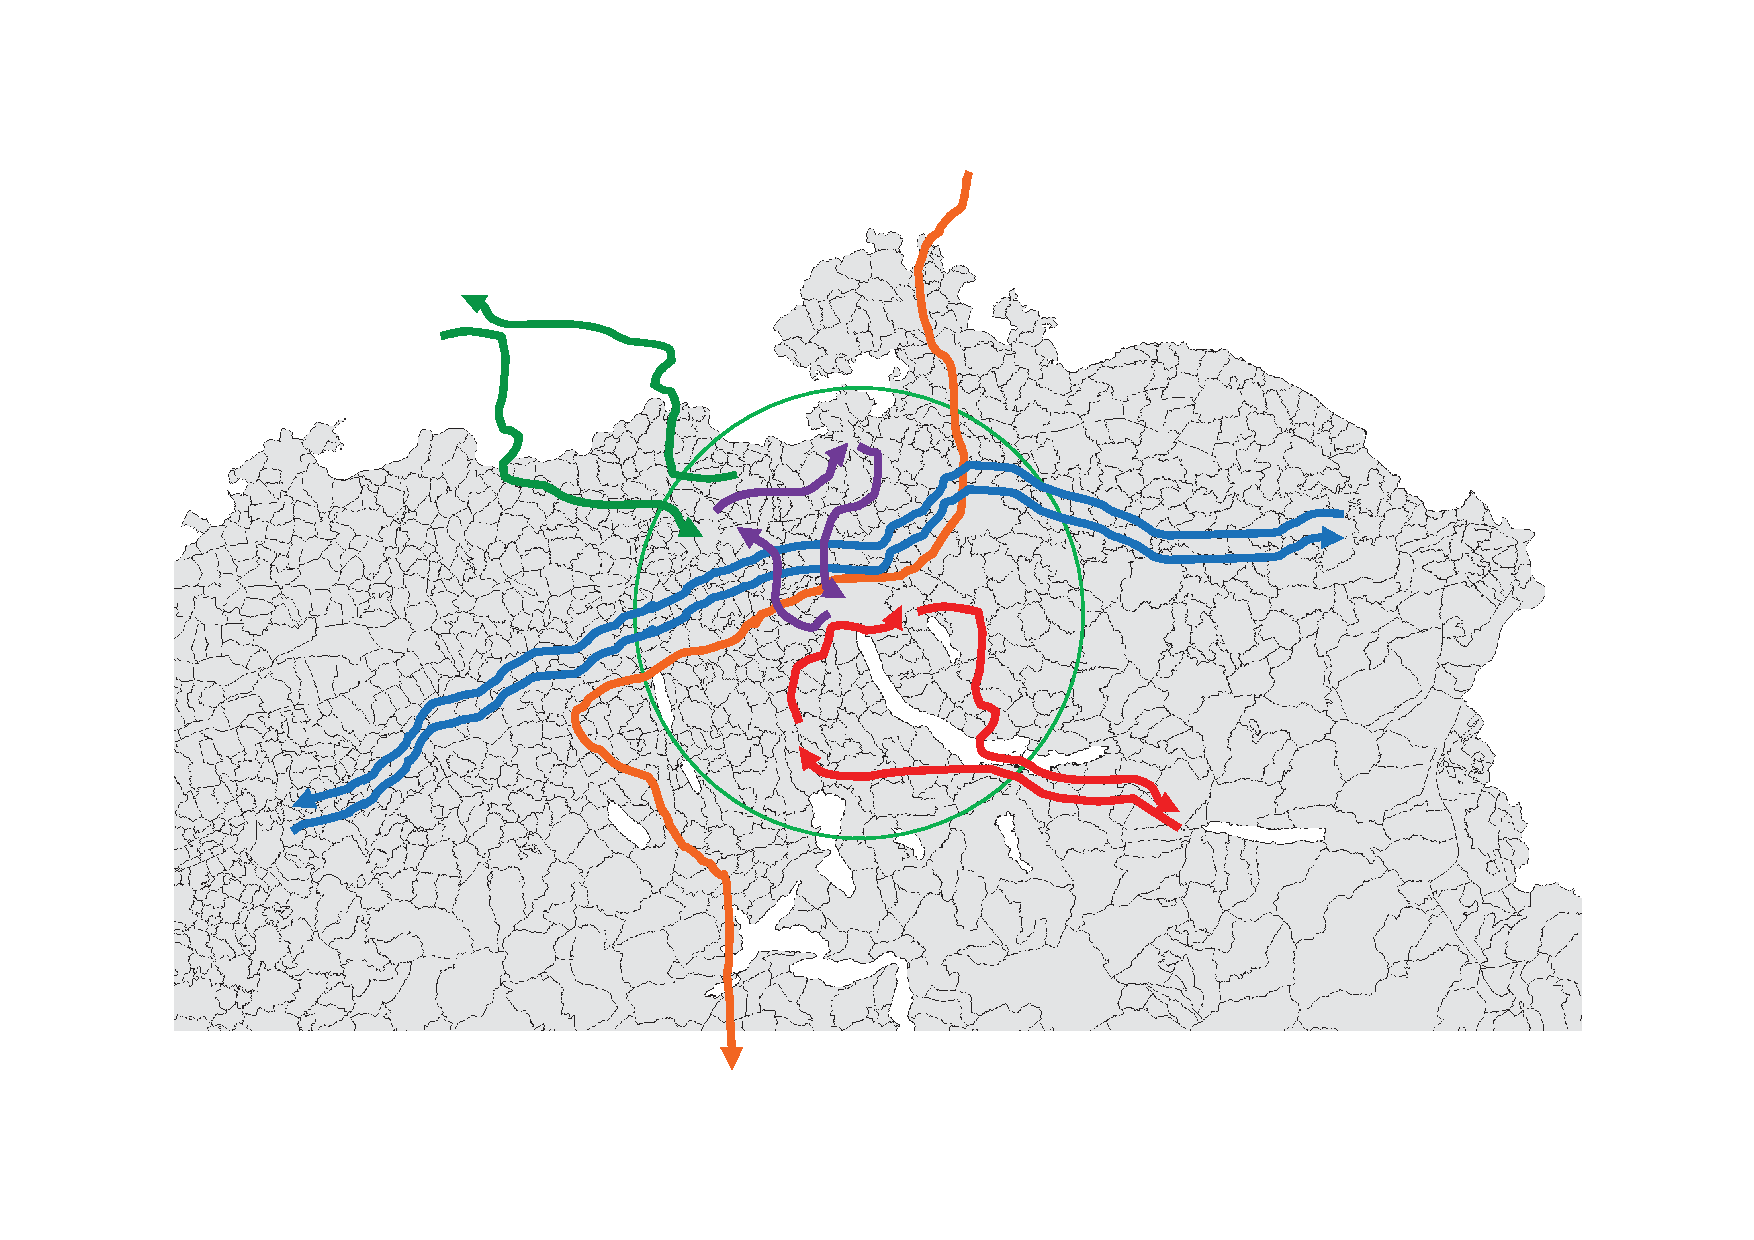
\includegraphics[width=0.99\textwidth, angle=0]{using/figures/zh.pdf}}%
{}

% ##################################################################################################################
 ok

% ==================================================================================================================
% ##################################################################################################################
\section{Singapore}
\label{sec:singapore}
\hfill \textbf{Authors:} Alexander Erath, Artem Chakirov

\editdone{This text has undergone the professional edit. Please no grammatical changes anymore! They are most-probably wrong.}

% ##################################################################################################################
The \gls{matsim} Singapore scenario \citet[][]{ErathEtAl_TechRep_FCL_forth} was implemented and is maintained at the \gls{fcl}, a research program of the \gls{sec} and part of Singapore's National Research Foundation \gls{create}. The scenario covered the whole Singapore area, with a population of approximately 5 million and included traffic  to and from neighboring Malaysia. Singapore provides an excellent study case for an agent- and activity-based modeling approach: a fairly densely populated city, with an extensive public transport infrastructure and advanced transportation and pricing policies. 

% ====================================================================================================
\subsection{Demand}
In the absence of a full-population census for Singapore, a synthetic population was generated based on data from the \gls{hits}~2008 \citep[][]{Choi_JOUR_2010} and population breakdowns of Singapore’s population census~2010. The synthetic population was derived using the fitting and sampling method \citep{MuellerKAxhausen_TRB_2011}, where a reference sample of household and person records was weighted, using an \gls{ipf} technique, until the weighted sample matched marginal census control totals. In our case, the reference sample was from travel survey records; fitting technique was the entropy optimization method proposed by \citet[][]{BarGeraEtAl_TRB_2009} and implemented by Kirill Müller, IVT, \gls{eth} Zürich. Then, the reference sample records were replicated through weighted sampling until the population total was met. 
 
Car ownership was modeled on a household level and driving licenses were assigned to individuals, using discrete choice methods. Given the high car tax in Singapore, the model reflected lower car ownership level than in other developed nations. The model presented in \citet[][]{VanEggermondEtAl_IATBR_2012} included not only socio-economic, but also spatial variables and proved to be essential to the \gls{matsim} Singapore model, leading to accurate mode choice and mode share predictions. 

Activity locations were defined on an individual building level, with  information on building and facility types compiled from various sources:i.e., the land-use master plan \citep[][]{URA_Rep_URA_2008}, government websites and online directories, as well as points of interest information provided by \gls{navteq}. In the absence of a business census, an innovative approach for location identification and corresponding number of work places was developed, drawn from the full smart card data record of public transport journeys and enriched with information on land-use and estimates of building floor space. In a first step, a probabilistic model was applied to a daily public transport journey record to identify types of activities performed between two subsequent public transport trips. Estimated and calibrated using HITS 2008 records, the model combined variables such as time of day, activity duration and land-use around each stop or station to ensure an accurate differentiation between home, work, or other activities. After accounting for mode shares in 53\,different zones, an optimization technique employing accessibility computation was applied to distribute work activities to individual buildings. More details on the newly developed methodology and its practical application were reported in \citet[][]{ChakirovErath_IATBR_2012} and \citet[][]{OrdonezErath_TRR_2013}. 

Assignment of households to buildings was performed using detailed information on residential developments; for public housing, which represented about 80\,\% of Singapore's residential building stock, information on distribution of different dwelling types was employed, while for privately owned condominiums, only information on number of apartments per building was available. Work locations were assigned using a zone-based gravity model using prior estimated number of work activities in each building as additional information for distribution of workplaces within each zone. Activity chains were assigned based on their observed frequency in \gls{hits}, taking into account key socio-demographic parameters like sex, age, occupation and income. Activity chains of type home~--~work~--~home were by far the most frequent, accounting for approximately 50\,\% of the trips.
Freight and cross border traffic, as well as tourist travel demand, were derived based on a set of origin destination matrices provided by the \gls{lta}. These matrices were converted into special daily plans. Information on the temporal distribution of freight trips was derived from loop detector data for freight and temporal attraction profiles of major tourist sites.

% ====================================================================================================
\subsection{Supply}
Using a semi-automatic map-matching algorithm~\ref{sec:networkeditor-singapore}, a high-resolution navigation network provided by \gls{navteq} was map-matched to, and enhanced with, \gls{lta}'s planning network lane and capacity information. Without access to traffic signal cycle time data, traffic lights were not specifically modeled. Extensive attention was paid to public transport modeling; interaction between private and public transport with Singapore’s high density and limited space was very important. Simulating dynamic effects, such as bus bunching, was crucial for obtaining realistic travel times and mode shares. Public transport network and schedule data provided by \gls{lta} included bus and train routes, as well as stop and station location. This information was matched to the road network, using yet another map-matching algorithm presented by \citet[][]{Ordonez_HKSTS_2011, Ordonez_Webpage_2011_4}. Recently, the scenario was updated using public transport schedule data derived from public transport smart card data records \citet[][]{Fourie_TechRep_FCL_2014}. Such schedule information provided actual vehicle dispatch frequencies and headways, which are continuously adjusted and, in some cases, can substantially deviate from published schedules. Additional features of public transport simulation in Singapore’s model included advanced bus dwell time model \citep[][]{SunEtAl_TransResA_2014}, as well as an approximation of the distance-based public transport fare scheme.

Other modes, specifically walking and cycling, were "teleported" with constant travel speeds without any interaction with other users. 

% ====================================================================================================
\subsection{Behavioral parameters}
Behavioral parameters specific to Singapore's context were borrowed from \citet[][]{LTA_unpub_2009} and used with the widely applied Charypar-Nagel function for activity scoring \citet[][]{CharyparNagel2005ga4acts}. Thus, the same parameters were used for all agents, ignoring user preferences heterogeneity and time values in the initial scenario implementation. Furthermore, no additional crowding penalties (impacting travelers' discomfort) were considered at this stage; public transport overcrowding effects were taken into account only with physical vehicle capacity limitations, as well as their implications for dwell time and the bus bunching phenomenon. 

% ====================================================================================================
\subsection{Policy}
The \gls{matsim} model for Singapore also included \gls{erp} scheme, featuring time and vehicle-dependent road pricing. Based on two data sets, with location and time-dependent price levels, prevailing tolls were specified for 73\,network links where toll gantries had been installed, as of February, 2012. To account for the numerous dedicated bus lanes, additional links attributed to exclusive bus use were added to the network. The existing links' capacity was reduced accordingly, even if, in some cases, dedicated exclusive bus lanes by buses existed only during peak hours. Such a simplified setup, insensitive to the time-dynamic operation of dedicated lanes, led to actual road capacity underestimation during periods when bus lanes were also open to other motorized traffic. However, as most links featuring bus lanes consisted of three or more lanes, the effect on modeled traffic conditions during off-peak hours appeared to be low.

% ====================================================================================================
\subsection{Calibration and validation}
Road usage data is available for around 200\, 
%\textbf{EXACT 200?} 
count stations at hourly intervals. Public transport smart card data availability provides an additional validation dimension. For the future,the opening of new \gls{mrt} lines---since setting up the model in 2012---presents a unique opportunity for comparing observed ridership with predicted ridership in the model. However, systematic calibration and detailed validation have not yet been conducted.

% ##################################################################################################################

% ==================================================================================================================
% ##################################################################################################################
\chapter{Munich}
\label{ch:munich}
\hfill \textbf{Author:} Benjamin Kickhöfer

\editdone{This text has undergone the professional edit. Please no grammatical changes anymore! They are most-probably wrong.}

% ##################################################################################################################
The \gls{matsim} scenario for the Munich metropolitan area was set up during 2010.%
%
\footnote{
%
Detailed descriptions of the scenario can be found in \citet{KickhoeferEtAl_VanoutriveVerhetsel_2013} and \citet{Kickhoefer_PhDThesis_2014}.
%
}
%
The main goal was, and is, simulation of local air pollutant and global greenhouse gas emissions and how their levels change with different policy measures---on aggregated and spatially disaggregated levels. Thus the scenario was used for development and testing of the \gls{emt} (see Chapter~\ref{ch:emissions}). For an example illustrating where overall $\mathit{NO_2}$ private car and freight vehicle emissions are produced over one day, see Figure~\ref{fig:munich:no2emissions}.
%
\createfigure%
{$\mathit{NO_2}$ emissions in Munich}%
{$\mathit{NO_2}$ emissions in Munich}%
{\label{fig:munich:no2emissions}}%
{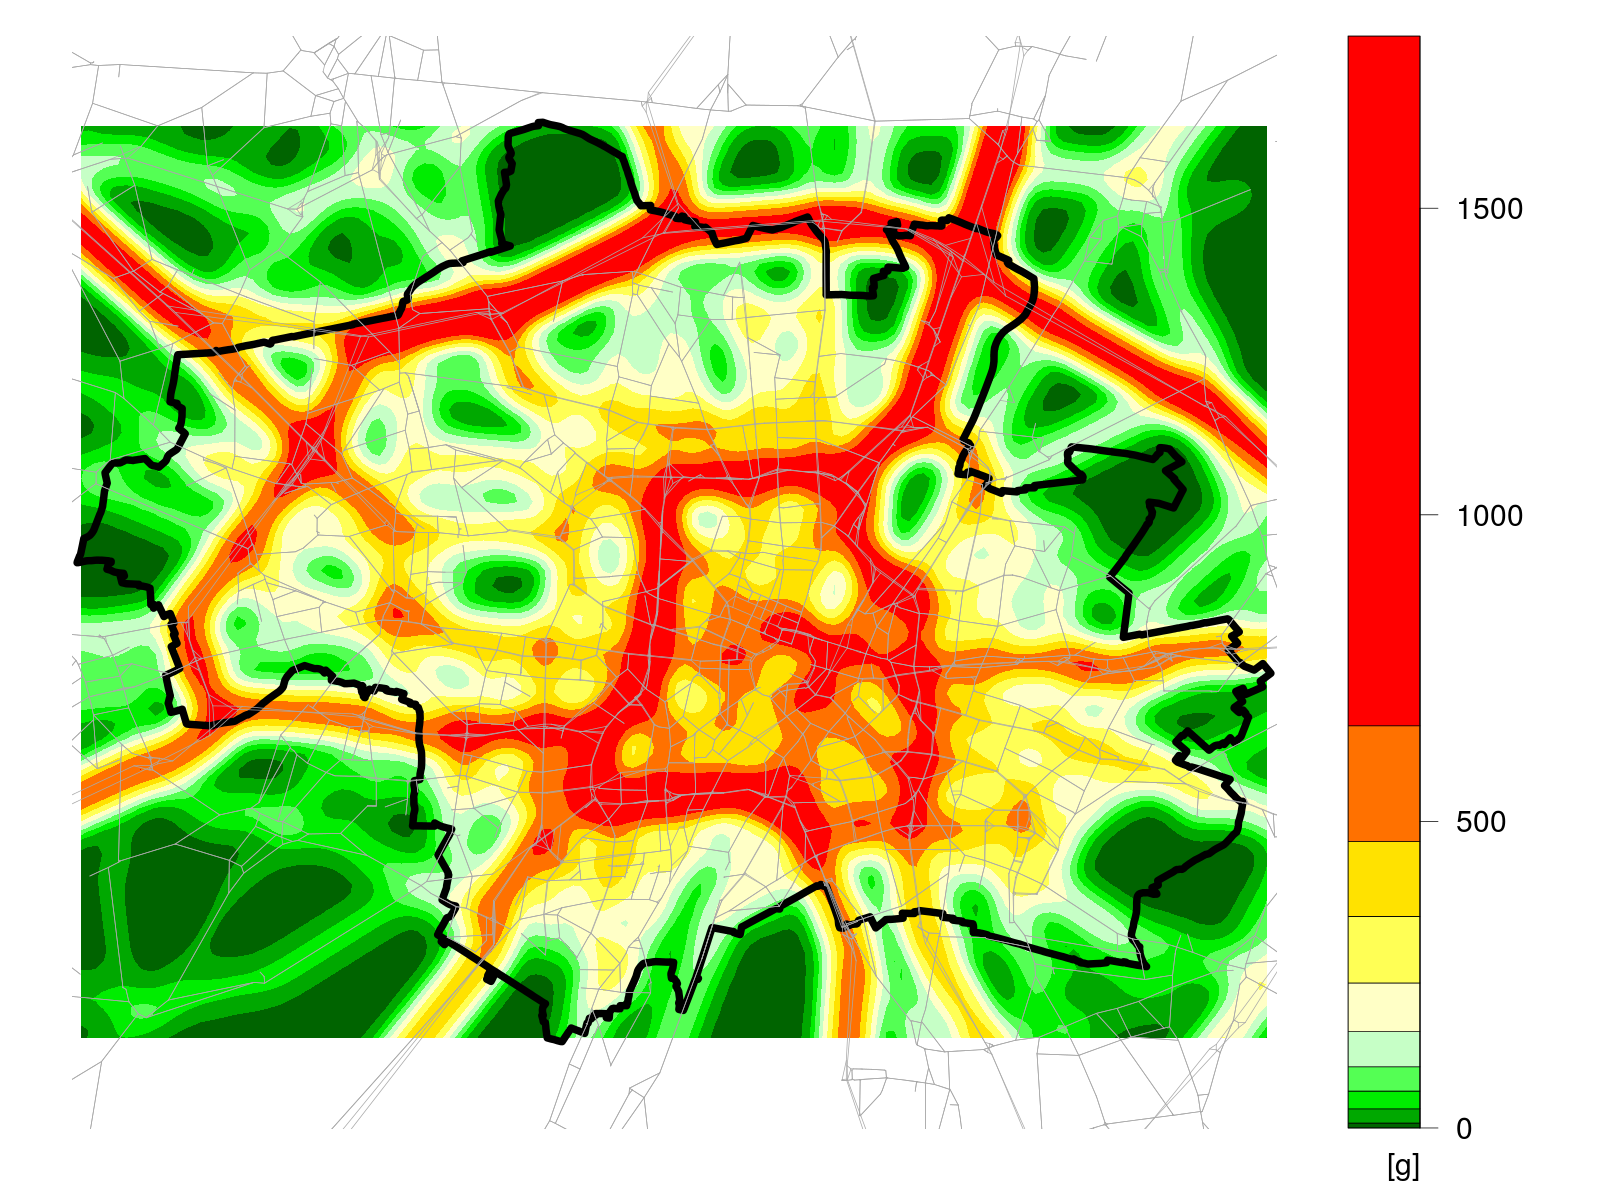
\includegraphics[width=0.85\textwidth, angle=0]{./scenarios/figures/baseCase_1500_NO2_g_108000_0.png}}%
{}

Network information from \acrshort{visum} was converted into \gls{matsim} format, resulting in a network of 17\,888 nodes and 41\,942 links.
%
This transport supply was then linked to travel demand from different sources; an inner-urban traffic activity-based demand from survey data was created, based on \gls{mid} \citep[MiD 2002,][]{FollmerEtAl_TechRep_infasDIW_2004}. This synthetic population segment consisted of roughly 1.4\,million individuals, with detailed vehicle information for every household.
%
Commuters and reverse commuters were modeled with data provided by the German Federal Employment Office \citep{BoehmeEigenhueller_TechRep_IAB_2006}. This part of the population consisted of approximately 0.5\,million individuals, with 0.3\,million commuting to Munich for work. The rest lived in Munich and commuted to their workplace around the city.
%
Freight traffic was also introduced into the model using data from the German Ministry for Transport \citep{ITBBVU_TechRep_2007}. This group consisted of roughly 0.15\,million freight vehicles, performing one commercial trip per day.

The scenario was used for several case studies:
%
\citet{HuelsmannEtAl_LAS_2011} used a single street corridor to validate simulated travel times and emission levels against actual data obtained from a test vehicle.
%
\citet{KickhoeferEtAl_VanoutriveVerhetsel_2013} investigated the relationship between the price elasticities of car travel demand and air pollutant emissions.
%
\citet{HuelsmannEtAl_GerikeEtAl_2013} identified city areas with high air pollution concentration. They defined these areas as ``hotspots'', exceeding the \gls{eu} limits for \gls{no2}. The authors raised toll levels incrementally for vehicles passing these hotspots, until high pollution concentrations disappeared, to estimate true threshold value \gls{eu} avoidance costs.
%
\citet{KickhoeferNagel2012EmissionInternalization} derived time-dependent, vehicle-specific, first-best air pollution tolls to create a benchmark for real-world policy evaluation.
%
\citet{KickhoeferKern_MobilTUM_2014} went one step further and calculated time-dependent, vehicle-specific air pollution exposure tolls to correct toll levels with \citet{KickhoeferNagel2012EmissionInternalization} for a count of individuals affected.



% ################################################################################################################## ok

% ==================================================================================================================
% ##################################################################################################################
\chapter{Sioux Falls}
\label{ch:siouxfalls}
\hfill \textbf{Author:} Artem Chakirov

\editdone{This text has undergone the professional edit. Please no grammatical changes anymore! They are most-probably wrong.}

% ##################################################################################################################
The Sioux Falls scenario provided a convenient test-case, combining fully dynamic demand fitted with realistic socio-economic and demographic attributes with a small-scale road network including an integrated public transportation system. Based on the Sioux Falls road network commonly used for tests and demonstration purposes in transportation literature \citep[][]{BarGera_TNTP_Webpage_2013}, it allowed quick and convenient experiments on new policy or software implementations with \gls{matsim} on a heterogeneous agent population, with a high degree of spatial resolution, but without significant computational requirements. However, it is important to stress that, despite the use of real world data for the generation of the enriched Sioux Falls scenario, it did not aim to replicate the real City of Sioux Falls in South Dakota, US and remains a fictitious test case. Detailed report on scenario generation and its characteristics is provided by \citet[][]{ChakirovFourie_TechRep_FCL_2014} and can also be found at \url{www.matsim.org/scenario/sioux-falls}. 

% ====================================================================================================
\section{Demand}
A realistic, socio-economically and demographically diverse demand population---with  heterogeneous use preferences---was crucial for unlocking the full potential of an agent-based simulation like \gls{matsim}. However, generation of a disaggregated demand description on individual and household levels close to reality was challenging; not only for trip origins and destinations, but also with respect to travel pattern relation and socio-demographic travelers' characteristics.

To address this challenge for the Sioux Falls scenario, and represent the household structure, demographic profile and income distribution as realistically as possible, a synthetic household population, using the \citet[][]{BarGeraEtAl_TRB_2009} entropy optimization technique, was generated. It matched the aggregate distribution of demographic attributes (age, sex and household income) recorded during the 2010 US Census. It contained census tracts inside, and adjoining, the city center of Sioux Falls and was composed of household and person records taken from the (anonymous) 5-year American Community Survey sample (2007-2011), covering 5\,\% of all households.

To keep the scenario accessible, as well as facilitating interpretation and understanding of possible effects on policies studied, only two simple activity chains were initially included: ``home – work – home'' and ``home – other – home''. Activity locations were identified using building stock data set provided by the City of Sioux Falls \gls{gis} division. Each household's home location was assigned randomly to a residential unit within the household's tract. Because no information on the real number and distribution of work places within the relevant area was easily accessible, the static \gls{od} matrix from \citet[][]{LeBlancEtAl_TransRes_1975} was taken as a workplace attraction indicator for each zone. Then, assignment of work places to individual workers, as well as locations of secondary (other) activities, was performed using a parameter-free radiation model presented by \citet[][]{SiminiEtAl_NAT_2012}.

To exploit the full potential of disaggregated demand and add another degree of realism to the scenario, car ownership on the household level was modeled using an ordered probit model, presented by \citet[][]{GiulianoDargay_TransResA_2006} and based on the \gls{npts}~1995. In addition to socio-demographic household characteristics (number of adults, children, pensioners, household income), the model used residential location attributes (population density, public transport access and dwelling type), which better described specific Sioux Falls scenario characteristics, as well as its area-wide bus network. 

% ====================================================================================================
\section{Supply} 
A realistic transportation test network should ensure sufficient complexity of travelers’ choice dimensions while limiting  computational effort. To this end, the Sioux Falls test network was introduced by \citet[][]{MorlokEtAl_ResRep_org-fhwa_1973} and later adapted as a benchmark and test scenario in many publications (see \citet[][]{ChakirovFourie_TechRep_FCL_2014} for overview). The network structure captured the major arterial roads of Sioux Falls, South Dakota, but was never intended to replicate the real city, or all characteristics of its transportation system, such as travel times or modal split. The original network was comprised of 76\,arcs, 24\,nodes and 552\,\gls{od} pairs. For this scenario, road capacities were adjusted according to values provided by the Highway Capacity Manual \citet[][]{HCM_2010} and other related research publications \citep[e.g.,][]{NgCFSmall_Transportation_2012}. The public transportation network added to the scenario included five bus lines, as initially proposed by \citet[][]{AbdulaalLeBlanc_TransScience_1979}, with bus stops placed at regular intervals of 600\,meters. 

Due to the design of \gls{matsim}’s queue simulation, agents were handled only at the beginning and end of each network link and could not enter or leave a link along its length. Therefore, origins and destinations located along very long links led to spatial detail loss, as all origins and destinations along the length of the link were effectively assigned the same coordinates. Consequently, to improve spatial detail level, all links of the Sioux Falls network were evenly split into smaller links, with maximum length of 500\,meters each. Following this operation, number of nodes was increased to 282 and number of links to 334, without changing effective network topology.

In addition to car and bus modes, walking as ``teleported'' mode, with constant travel speeds, and with no interaction with other users, is used as the non-motorized transportation mode. 

% ====================================================================================================
\section{Behavioral Parameters}
Behavioral parameters used in utility functions were based on estimated demand model for Sydney by \citet[][]{TirachiniHensherRose_TransResB_2014}. Before applying parameters in an activity-based context, time-related parameters had to be adjusted to account for utility gained from activity performance. Thus, to provide a value for marginal utility of performing an activity, the travel mode with smallest the disutility was set as a baseline, under the assumption that traveling with this mode was equivalent to idling/doing nothing. Corresponding parameters were split into opportunity costs of time and a mode-specific disutility of traveling, as has in previous \gls{matsim}-related publications as \citet[e.g,][]{KickhoeferEtAl_Transportation_2011}. 

% ====================================================================================================
\section{Results, Drawbacks and Outlook}
Sioux Falls scenario stability and performance was tested using two sets of activity timing constraints, as well as five different random seeds, which all delivered stable and realistic results. \citet[][]{ChakirovFourie_TechRep_FCL_2014} also investigated \gls{mfd} existence and hysteresis characteristics, as discussed in \citet[][]{GeroliminisDaganzo_TRB_2007, GeroliminisDaganzo_TransResB_2008, GeroliminisSun_TransResA_2011}. 

However, recent experience has shown certain coarse network drawbacks; it represented only major arterial roads and neglected minor neighborhood and collector road links. With an elaborate synthetic population and high rush hour demand peaks, the network seemed to be sensitive to network breakdowns under high loading conditions. 

Along with the coarse road network, the coarse public transport network level and the resulting  low level of accessibility (for parts of the population) represented another drawback, particularly relevant to simulation and evaluation of policies sensitive to, or requiring, a certain share of public transport users. 

Replacing the original Sioux Falls network with a finer network obtained from the crowd-sourced \gls{osm} and adding additional public transport lines would address the above-mentioned scenario weakness. However, this introduces a different set of drawbacks and would require further attention. First, the significantly larger number of network links and nodes increases time and resources for routing and dynamic queue simulation and could erase the advantages of a small-scale network. Extended simulation times can be tackled with the new pseudo-simulation methodology, currently developed by \citet[][]{FourieEtAl_TRR_2013}.
Second, total network capacity increase leads to reduction or even disappearance of congestion during peak hours, although including freight and through traffic in the scenario can make it more realistic and address congested conditions during peak-hours. 

% ##################################################################################################################
 ok


% ==================================================================================================================
% ##################################################################################################################
\section{Barcelona}
\label{sec:barcelona}
\hfill \textbf{Author:} Miguel Picornell

% ##################################################################################################################
The Barcelona scenario is one of the three case studies (together with London and Zürich) carried out under the framework of the \gls{eunoia} project. The main goal of the Barcelona case study is to evaluate the impact of different public bike-sharing schemes in the city. The study area covers the metropolitan area of Barcelona, with special focus on the city center, where public bike-sharing stations are located. For this study a novel bike-sharing module was developed by \gls{eth} Zürich.

% ===================================================================================
\subsection{Transport Supply: Network and Public Transport}
The road network has been extracted from the \gls{transcad} model used by the city of Barcelona. Public transport supply has been also considered, comprising: bus, underground, tram, train and bike-sharing. Information about stops and schedules has been obtained from the public information available at the Barcelona Open Data platform as well as from the Barcelona transport authority website. 

% ===================================================================================
\subsection{Transport Demand: Population} 
Agent plans have been defined using anonymised mobile phone registers \glspl{cdr}. From mobile phone data it is possible to identify places where the agents perform activities and their corresponding trips derived from those activities. Activities have been classified as "home", "work" and "other" (including as "other", "leisure", "shopping", etc.). A sample of around 15\,\% of the population has been used in the simulation. Walk, cycling, public transport and car are the modes included in the simulation model.

% ===================================================================================
\subsection{Calibration and Validation}
Different data sources have been used to calibrate and validate the model. First, in order to validate the agent plans obtained from mobile phone data, results were compared to \gls{emef}, leading to conclude that mobile phone data provide similar information than traditional surveys. Additionally, agent’s utility function has been calibrated using the modal split from \gls{emef} and road counts.

% ===================================================================================
\subsection{Results and More Information}
At the time this summary was written, the calibration process ongoing. More detailed information about the scenario and main results can be found at:
\url{www.eunoia-project.eu/publications/} (project deliverables/Report on Case Study 3: Barcelona).

% ##################################################################################################################
 ok

% ==================================================================================================================
% ##################################################################################################################
\chapter{Brussels}
\label{ch:brussels}
\hfill \textbf{Author:} Daniel Röder

\editdone{This text has undergone the professional edit. Please no grammatical changes anymore! They are most-probably wrong.}

% ##################################################################################################################
The \gls{matsim} scenario for Brussels was developed as part of the \gls{sustaincity} project. This project's goal was to couple an urban land use model, in this case \gls{urbansim}, with the \gls{matsim} mobility simulation, to evaluate transport policy impact on urban land use and vice versa. A detailed description of this coupling is given by \citet{Nicolai2013PhD} and others. A detailed description of the scenario development is found in \citet{RoederNagel2013SketchPlanningBrussels}.

The scenario covered the greater Brussels area in Belgium; input data was derived from two main sources. The population was directly generated from the \gls{urbansim} model, covering a total of 860\,214 persons. At home- and at work-locations (per person) were given and converted into a daily home-work-home plan. For computational reasons, a randomly-drawn population sample of one percent was used. \gls{osm} was sourced for the street network generation, which consisted of 10\,861 nodes and 19\,830 links, \ie using mainly the trunk road network.

For the modeling of public transport, two different approaches were tested:  first, the \gls{matsim} default approach for scenarios where no detailed transit schedule is available, based on either: beeline distance and average speed, or network-based freespeed travel times and a designated factor. The second approach was not part of the \gls{matsim} core during the project, but was available as a contribution (\lstinline|matrixBasedPtRouter|). It was based on \gls{od} travel time matrices between transit stops, \ie travel times for all relations were computed in a pre-process. The travel times can based on a real-world-schedule or certain assumptions which can take spatial coverage into account. Advantages of this model are obvious; on one hand, it may depict spatial coverage with public transport supply---here, distance to the next transit stop influences travel time. On the other hand, it may depict the real network, \ie routes and lines and possible waiting times for switching. Both approaches were compared against travel times and mode share measures from a \gls{saturn} model. Since the matrix-based approach came closer to this model, further investigations were based on that.

To evaluate the model's sensitivity to certain policies, a cordon toll scenario was set up, where a toll is charged between 6 and 10\,am every time a car passed a cordon border. \ie every time a car entered a link crossing a cordon border defined by the Brussels freeway ring. Accessibility was calculated and compared for both scenarios.  \citet{RoederNagel2013SketchPlanningBrussels} provides a detailed analysis.

% ##################################################################################################################
 ok

% ==================================================================================================================
% ##################################################################################################################
\section{Cape Town}
\label{sec:capetown}
\hfill \textbf{Author:} Johan Joubert

% ##################################################################################################################
https://matsim.atlassian.net/wiki/display/MATPUB/South+Africa

% ##################################################################################################################

% ==================================================================================================================
% ##################################################################################################################
\chapter{Cottbus: Traffic Light Simulation}
\label{ch:cottbus} \hfill \textbf{Authors:} Joschka Bischoff, Dominik Grether \editdone{This text has undergone the professional edit. Please no grammatical changes anymore! They are most-probably wrong.}

% ##################################################################################################################
The Cottbus (Germany) scenario (Figure~\ref{fig:scenarios:cottbus_location}) is used for traffic light simulation (see Chapter~\ref{ch:signalslanes}). 
It is explained well in \citet[][pp.~87]{Grether_PhDThesis_2014}; this chapter briefly reviews the main points. 
The scenario data is generally available to the public.

The network is derived from \gls{osm} data in summer, 2010 \citep{Bischoff2010BaSylvia} and 
covers all streets within the city boundaries, as well as main roads in the surrounding Spree-Neiße administrative district . 
It is designed as a 100\,\% sample. 
The population is based on the German federal employment agency commuter statistics for both Cottbus and Spree-Neiße \citep{WiethoelterBogaiCarstensen2010IABPendlerberichtBB}. 
As such, the population has only home-work-home plans spread over the usual commuting times, resulting in two peaks, including 
33\,479 agents traveling exclusively by car. 
The scenario is generally not very busy; the area does not usually have major congestion issues.

Figure~\ref{fig:network_municipalities_cottbus_landuse} shows the network over the 
``Corine Land Cover'' landuse \citep{CorineLandCover2006Data}, provided by European Environmental Agency. 
Woods and agricultural areas are depicted; most of the region is agricultural use area.  
Virtual persons in \gls{matsim} need a geographic coordinate for their activities. 
If this coordinate is drawn randomly (solely based on municipality borders), home and work activity locations are uniformly distributed over  the area, \ie most of them in woods and fields. 
Thus, activity locations are drawn randomly in combination with land use data. 
The coordinate must be in the municipality area and for home activity, it must be located in urban fabric areas; for work locations, industrial or commercial areas are also allowed. 
The resulting home activity locations are shown in Figure~\ref{fig:cottbus_population_home}. 

The scenario contains data for 22\,traffic signals within the city center, based on the city's 2009~signal plans; junction layout is also modeled in detail. Fixed-time control data is taken from \citet{KoehlerStrehler2010SignalDemandOptimization}.  
Due to higher transport network resolution, several originally recorded fixed-time control schedules are invalid and were removed; data for 22\,junctions is available. 
Figure~\ref{fig:cottbus_network_signal_locations} shows their transport network location.  

Public transit, not part of the original scenario, is available based on 2011~schedules, although it is not currently used. 
%\createfigure%
%{Cottbus scenario: Geospatial location within Germany, Europe}%
%{Cottbus scenario: Geospatial location within Germany, Europe}%
%{\label{fig:scenarios:cottbus_location}}%
%{%
%  \createsubfigure%
%	{Geospatial area of Brandenburg within Germany, Europe (Red); City of Berlin (Yellow)}
%	{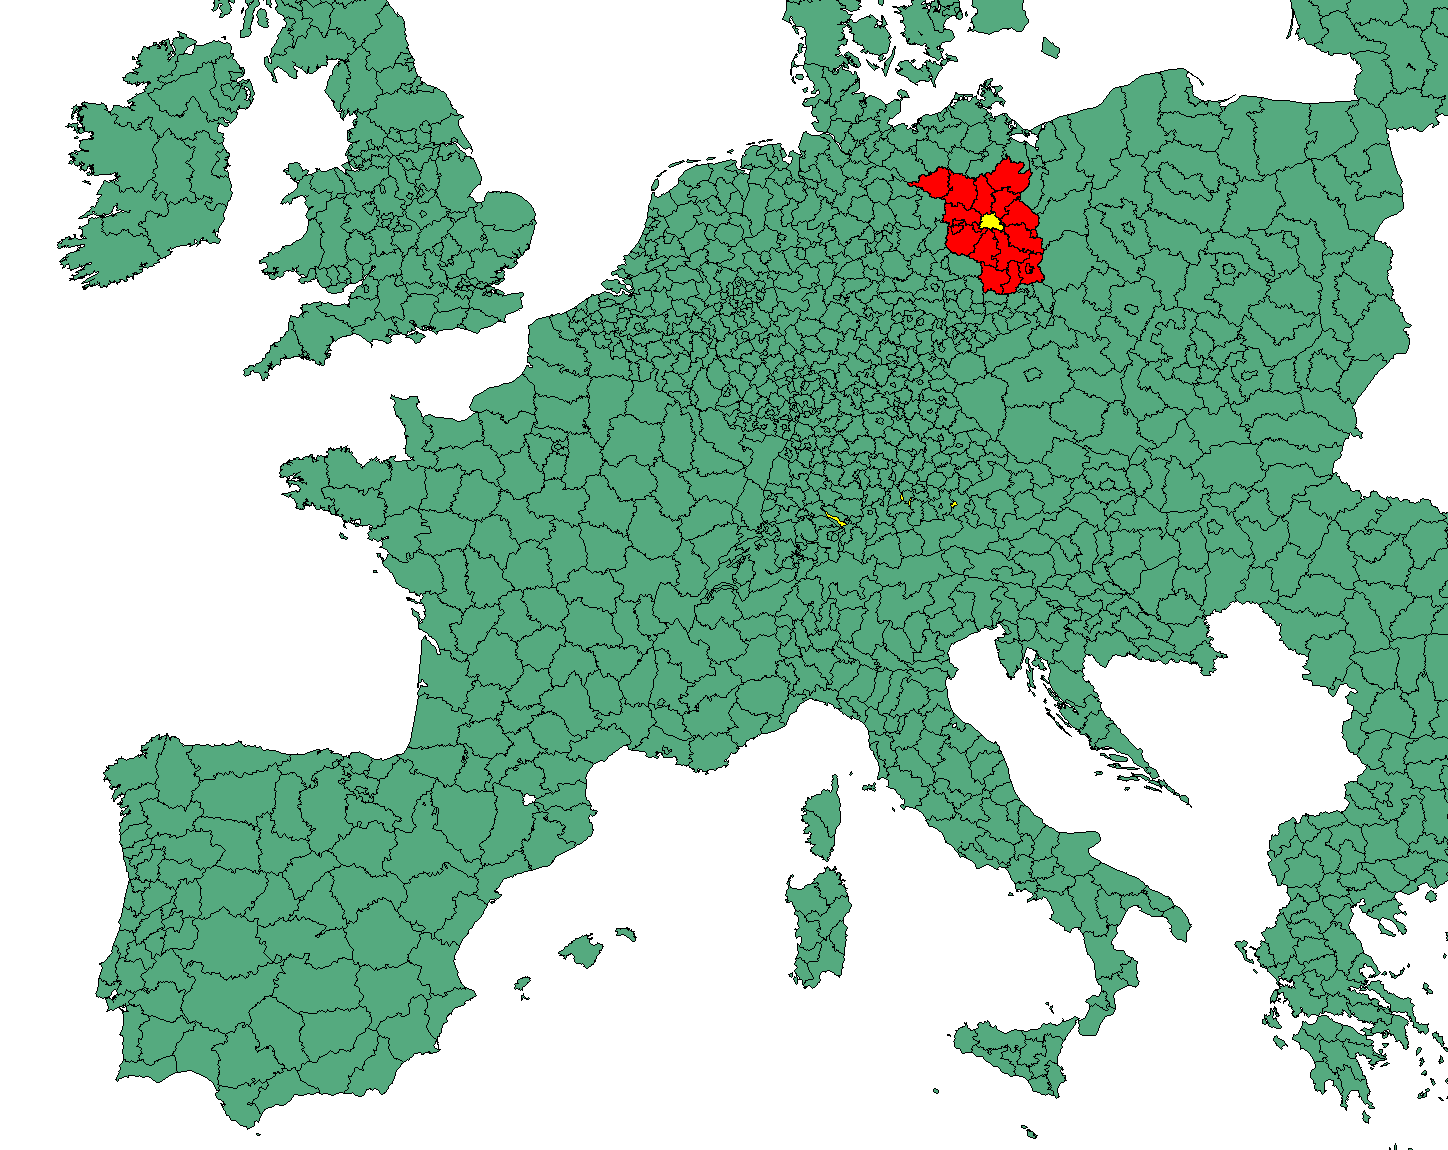
\includegraphics[width=0.49\textwidth]{./scenarios/figures/brandenburg_europe.png}}
%	{\label{fig:scenarios:cottbus_brandenburg_europe}}
%  \createsubfigure%
%	{Geospatial area of Cottbus (Dark Red), within administrative district Spree-Neiße, Brandenburg (Light Red)}
%	{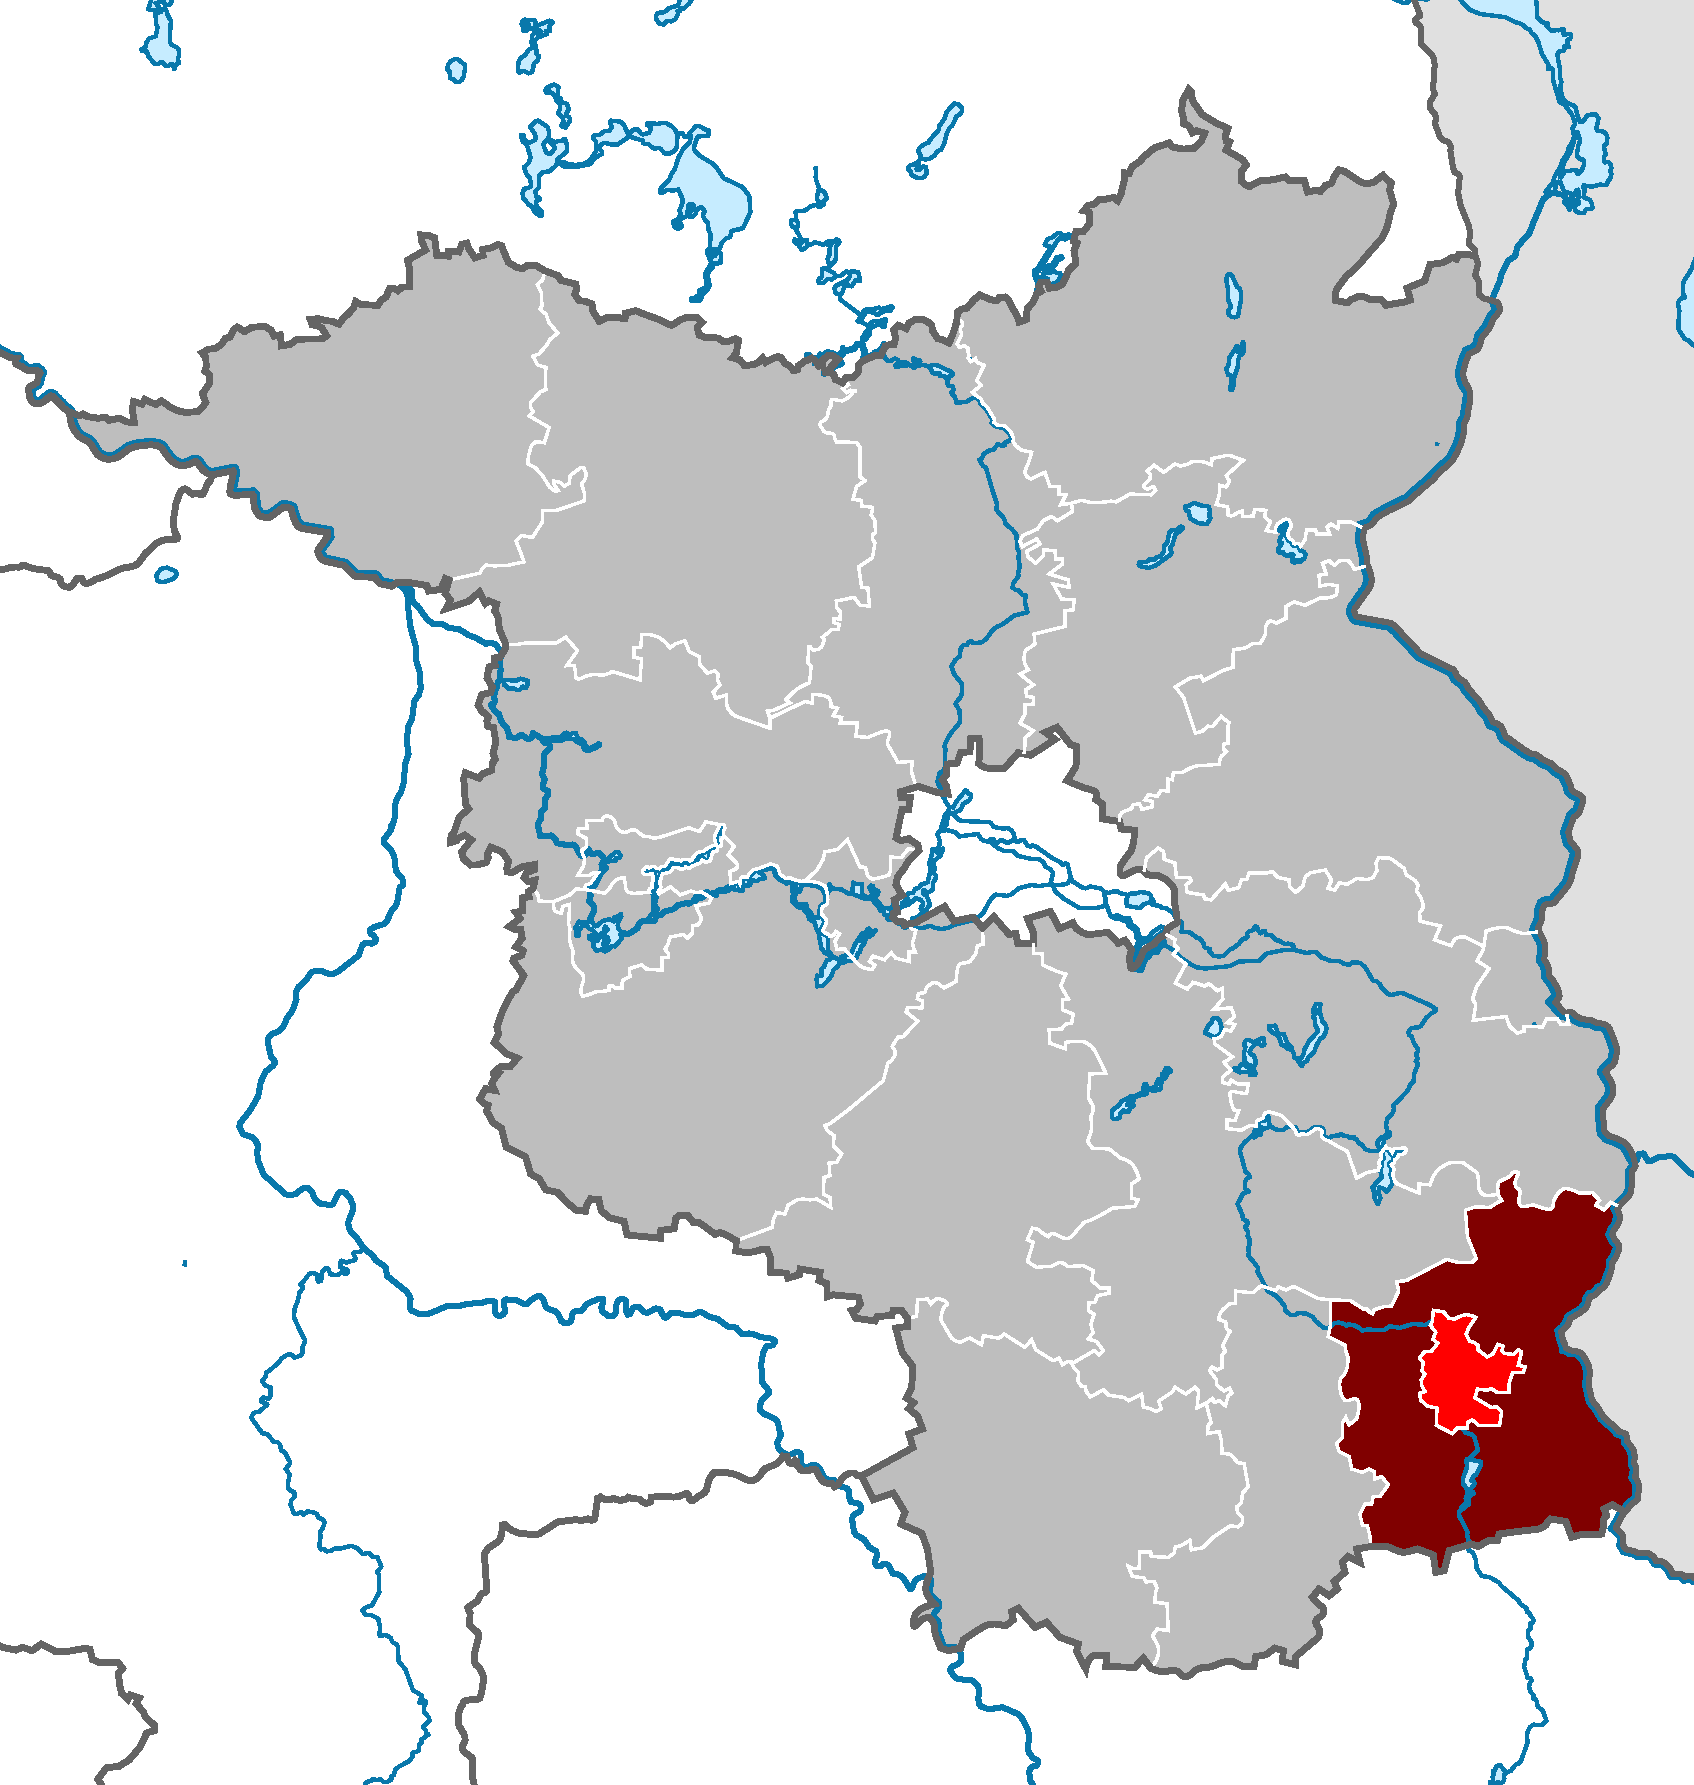
\includegraphics[width=0.49\textwidth]{./scenarios/figures/brandenburg_spree_neise_cottbus.pdf}}
%	{\label{fig:scenarios:cottbus_bb}}
%}%
%{\citet{Grether2014PhD}}

\createfigure%
{Cottbus scenario: Network and population}%
{Cottbus scenario: Network and population}%
{\label{fig:cottbus_network_population}}%
{%
  \createsubfigure%
	{Cottbus network and municipality borders}
	{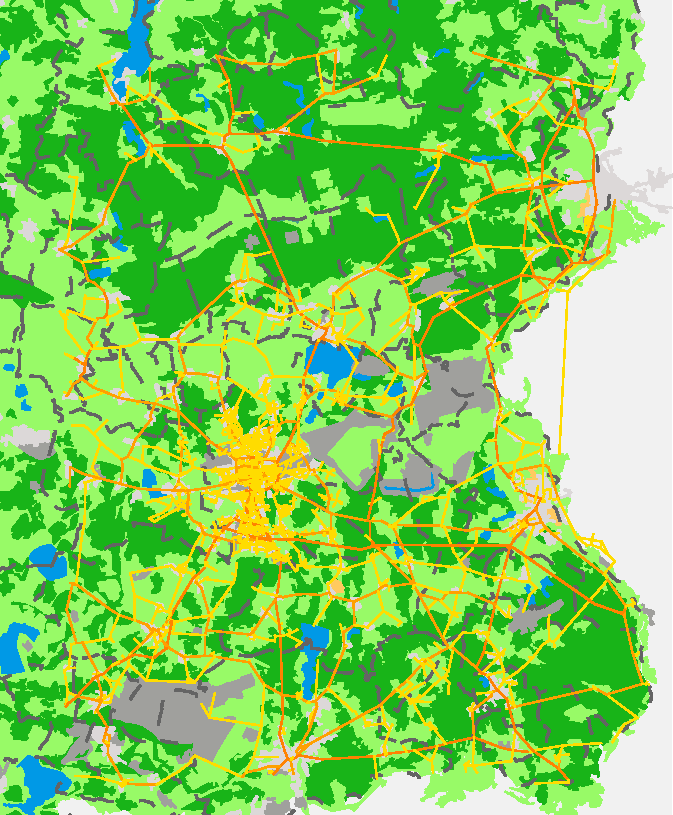
\includegraphics[width=0.49\linewidth]{./scenarios/figures/2013_network_gemeinden_landuse_edit.pdf}}
	{\label{fig:network_municipalities_cottbus_landuse}}
  \createsubfigure%
	{Synthetic population for the Cottbus scenario, geospatial location of home activities}
	{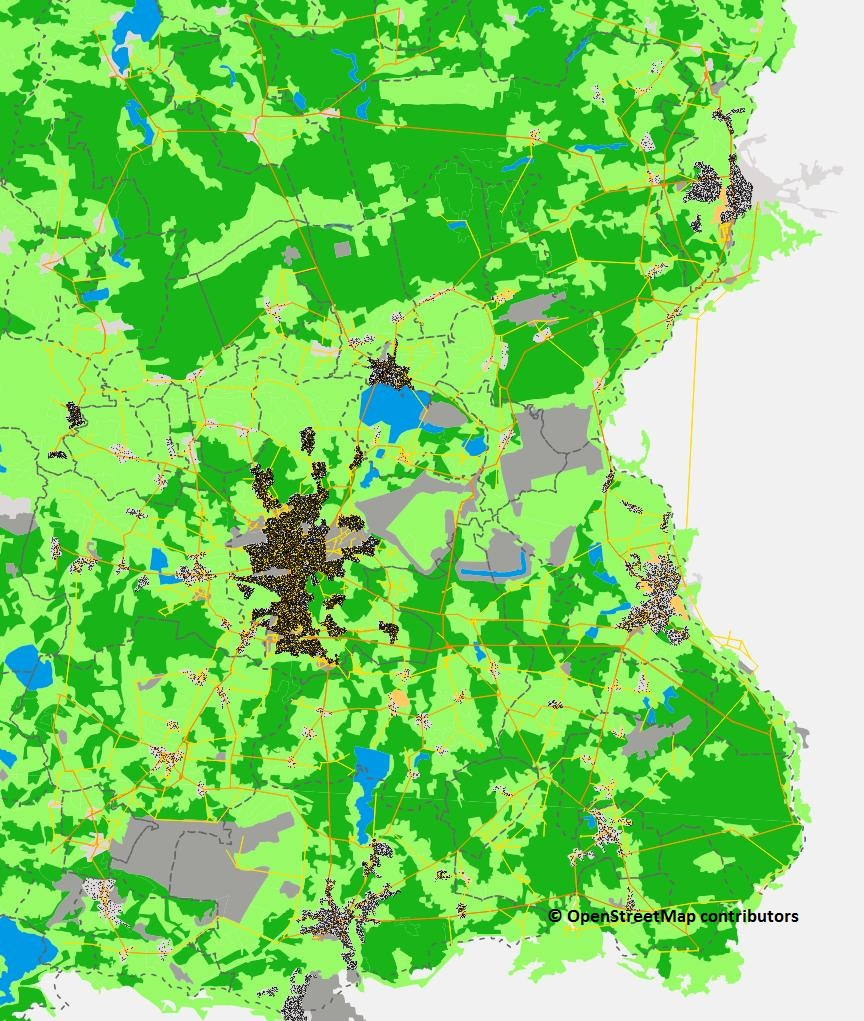
\includegraphics[width=0.49\linewidth]{./scenarios/figures/2013_network_gemeinden_landuse_population_home.jpg}}
	{\label{fig:cottbus_population_home}}
}%
{Source:~\citet{Grether2014PhD}} 

\createfigure%
{Cottbus scenario: Network, area with traffic signals within the city of Cottbus}
{Cottbus scenario: Network, area with traffic signals within the city of Cottbus}
{\label{fig:cottbus_network_signal_locations}}
{%
  \createsubfigure%
	{Location within city of Cottbus}
	{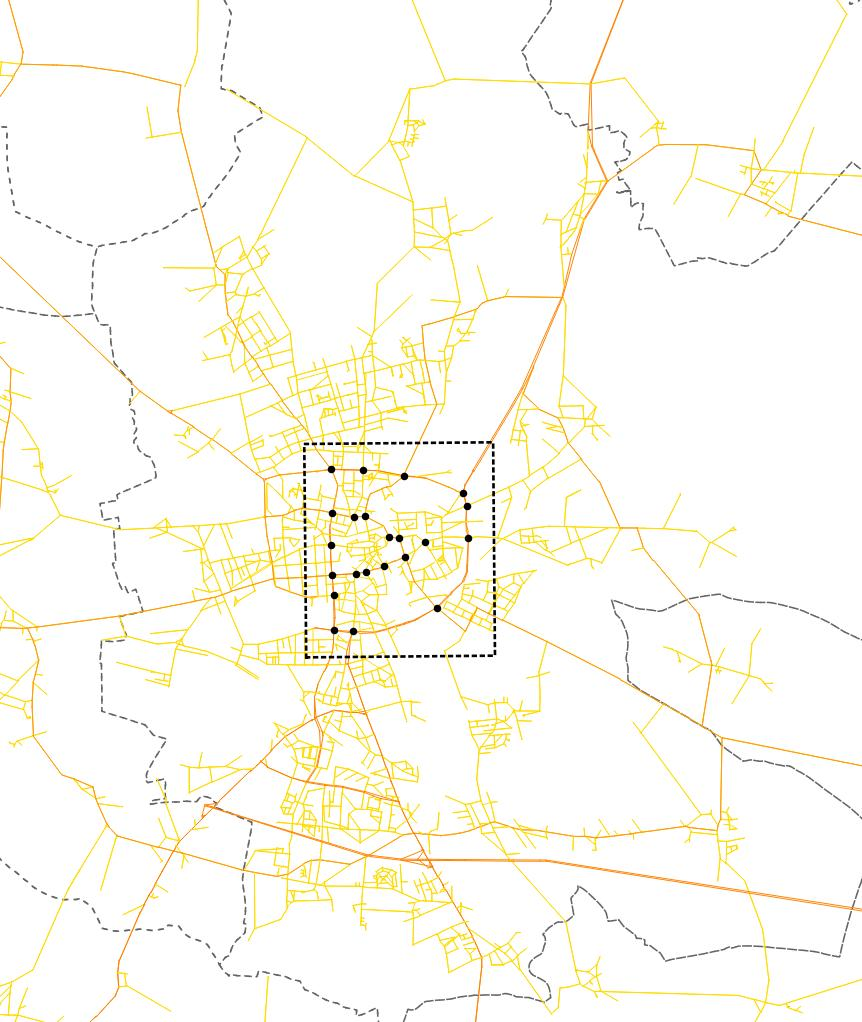
\includegraphics[width=0.49\linewidth]{./scenarios/figures/2013_cottbus_network_signals.jpg}}
	{\label{fig:cottbus_network_signals}}
  \createsubfigure%
	{Signalized area in detail}
	{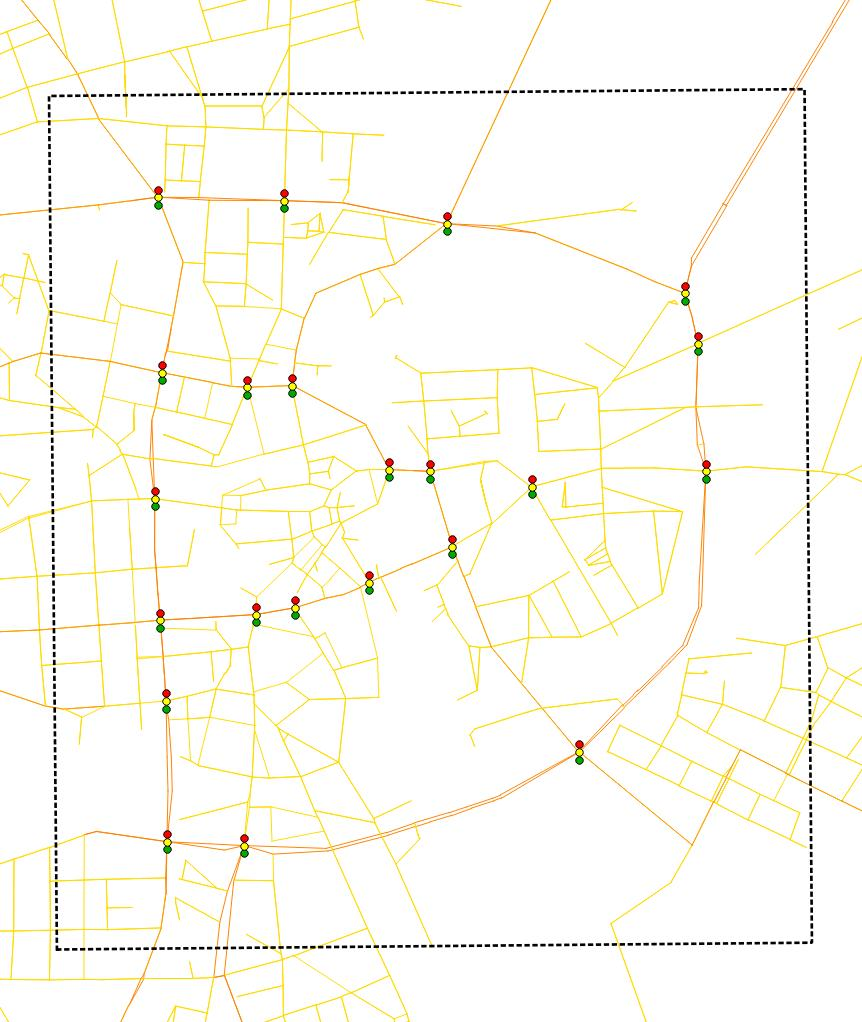
\includegraphics[width=0.49\linewidth]{./scenarios/figures/2013_cottbus_network_signals_zoom.jpg}}
	{\label{fig:cottbus_network_signals_zoom}}
}%
{\citet{Grether2014PhD}}

% ##################################################################################################################

% Andreas Neumann-Mail: frei verfügbar. ÖV vorhanden, 100\% Szenario, das sich mit einigermassen geringem Aufwand rechnen lässt. Grundlage für Dominik G.s Ampelpart
 ok

% ==================================================================================================================
% ##################################################################################################################
\section{Dublin}
\label{sec:dublin}
\hfill \textbf{Authors:} Gavin McArdle, Eoghan Furey, Aonghus Lawlor, Alexei Pozdnoukhov

\editdone{This text has undergone the professional edit. Please no grammatical changes anymore! They are most-probably wrong.}

% ##################################################################################################################
\subsection{Introduction}
To demonstrate a new spatial choice model, a micro-simulation of urban traffic flows for the greater Dublin region was implemented using \gls{matsim}. The scenario simulated leisure activities and commuting trips completed by individuals using private cars over a twenty-four hour period. For commuting trips, detailed information from the Irish Census was used; a new spatial choice model, inspired by the radiation model, was developed for leisure trips. The effectiveness of the approach was validated using hourly data from count stations on the main motorways around Dublin City. The results show that the micro-simulation accurately reproduced traffic volumes.

% =======================================================================================
\subsection{Study Area}
County Dublin, in Ireland, covers an area of approximately 115\,square kilometers and encompasses several administrative areas. Dublin is a coastal county with the Irish Sea lying to the east. To capture both intra-city and inter-city flows, the scenario considered individuals who live or work in Dublin, capturing those who commute to or out of Dublin, as well as those who live and work there.

% =======================================================================================
\subsection{Network}
To capture the desired study area for the scenario, the network consisted of all roads in the greater Dublin region and major roads for the remainder of the county. The road network was a mix of motorway, national routes and local roads and was extracted from \gls{osm}, along with other information such as speed limits and number of traffic lanes. This \gls{osm} network was prepared for use in \gls{matsim}.  This study focused on private vehicles; the public transport network was not considered, but can be incorporated into the micro-simulation in future studies.

% =======================================================================================
\subsection{Population Generation}
The population for this scenario consisted of all car drivers who live or work in the greater Dublin region and was prepared from a variety of data sets. To obtain home and work locations, the 2011 Irish census was used, particularly census subset \gls{powscar}. This provided home and work locations, mode of commuting transport used, time of departure for work or school and a variety of socio-economic data at an individual level. The individuals relevant to this scenario (drivers who live or work in Dublin) were extracted from the data set. In \gls{powscar}, home locations were anonymized by aggregating them into a statistical unit called the small area, consisting of 80 to 100\,households.  In the greater Dublin region, this represented a street or an apartment complex. We translated this to an individual address point by selecting a random address point within the small area. For this process, we used a commercial database of addresses and their coordinates in Ireland called Geodirectory. To account for non-workers, we used census statistics on spatial distribution of the number of sick, unemployed, retired persons and car ownership to produce the non-working population for the greater Dublin region. These were also assigned to individual address points, providing us with a population of 600\,000 agents for the scenario (see Figure~\ref{fig:dublin0}).

% ======================================================================================= 
\subsection{Demand Generation}
Individuals from the population were assigned work and school locations according to \gls{powscar} (Figure~\ref{fig:dublin0}). In \gls{powscar}, work and school locations were given at a 250\,meters grid level and then translated into an individual address point using Geodirectory. For school and collage locations, the address point was checked using \gls{nace} Codes, to confirm its status as an educational institute. Departure times for work  and school were assigned using a Gaussian curve centered at the declared 30\,minute departure time from \gls{powscar}.  \gls{ints} was used to create non-commuter demand for the road network. Through a survey, the \gls{ints} collected a 24\,hour travel diary for an Irish population sample recording journey origin, destination, departure time and mode. We extracted the private car mode and combined the data with the commuter data to create a 24\,hour activity chain for each individual in the population.

% ======================================================================================= 
\subsection{Activity Locations}
A set of activity locations were obtained from an in-car navigation system’s \glspl{poi} database and augmented with additional \glspl{poi} from \gls{osm}. While work locations were assigned from demand generation, locations for secondary activities, such as shopping and leisure, were not specified in the \gls{ints} and so had to be modeled to create spatial and temporal activity chains for the population. We developed a radiation model variant that applied emission-absorption ideas to compute interaction probabilities for a set of origins and destinations. The radiation model was parameter-free and distance decay was replaced by a ranked-based decay \citep[][]{SiminiEtAl_NAT_2012}. While generally used for modeling movement between regions or cities, we used this approach to produce probabilities of selecting different locations capable of fulfilling a given activity. Where the radiation model uses known populations of locations to produce region ranking, we used attractiveness scores for areas and facilities that could fulfill an activity. A facility, venue or area's attractiveness was derived from venue size, which was calculated using domain knowledge and the model was calibrated with trip distribution patterns from social media check-in statistics. This radiation model variant was used to assign locations to secondary activities in the agents’ day chains for the Dublin scenario demand.

% ======================================================================================= 
\subsection{Validation and Results}
Network, population and demand data were prepared for use with \gls{matsim}. For efficiency reasons, a 25\,\% sample of the population was used for the simulation. The location choice model described above was used to generate the initial demand. On each interaction of the simulation, agents could be rerouted or rescheduled according to the \gls{matsim} default settings, but the locations defined in activity chains remained constant. The simulation reached a stable state after 350\,iterations. The road volume data output was scaled according to the sample used, aggregated to an hourly count and compared to the observed count data from 6\,count stations on motorways around Dublin. In order to compare the effect of the new location choice model, the simulation was re-run using the \gls{matsim} nearest neighbor algorithm for selecting secondary activities' locations.

% =======================================================================================
\subsection{Achieved Results}
Aggregated hourly counts were compared with those observed at the 6\,count stations which determine vehicles traveling in two directions. A typical hourly distribution was obtained by averaging mid-week traffic volumes for a 3\,month period. The results produced by the radiation model showed a stronger correlation between simulated and observed counts than those from the nearest neighbor approach. Figure~\ref{fig:dublin1} showed hourly observed and simulated count data for two count stations; the inset showed relative percentage error for the two approaches being tested. The results indicated that both techniques were effective for estimating commuter traffic during morning and evening peaks. This was to be expected as the location of school and work activities were provided from real world data, but it did confirm the \gls{matsim} routing algorithm effectiveness For daytime traffic, which consisted mostly of secondary activities, our variant of the radiation model outperformed the nearest neighbor approach; it included individuals who were willing to travel further for better opportunities, producing more accurate results.

% =======================================================================================
\subsection{Associated Projects and Where to Find More}
The Dublin scenario validation results demonstrated the effectiveness of \gls{matsim} as a traffic simulation tool and also showed the power of our spatial choice model which adapted the radiation model to predict individual movement at a small spatial scale. In the future, the research will be expanded by considering a \gls{multimodal} transport network and scaling the scenario from an urban simulation to a national one. Full details of the Dublin scenario can be found in \citet[][]{McArdleEtAl_IWUC_2012} and \citet[][]{McArdleEtAl_ACMTIS_2014}.

% =======================================================================================
% ------------
\createfigure%
{The distribution of work and home locations for part of the Dublin scenario}%
{The distribution of work (upper image) and home (lower image) locations for part of the Dublin scenario}%
{\label{fig:dublin0}}%
{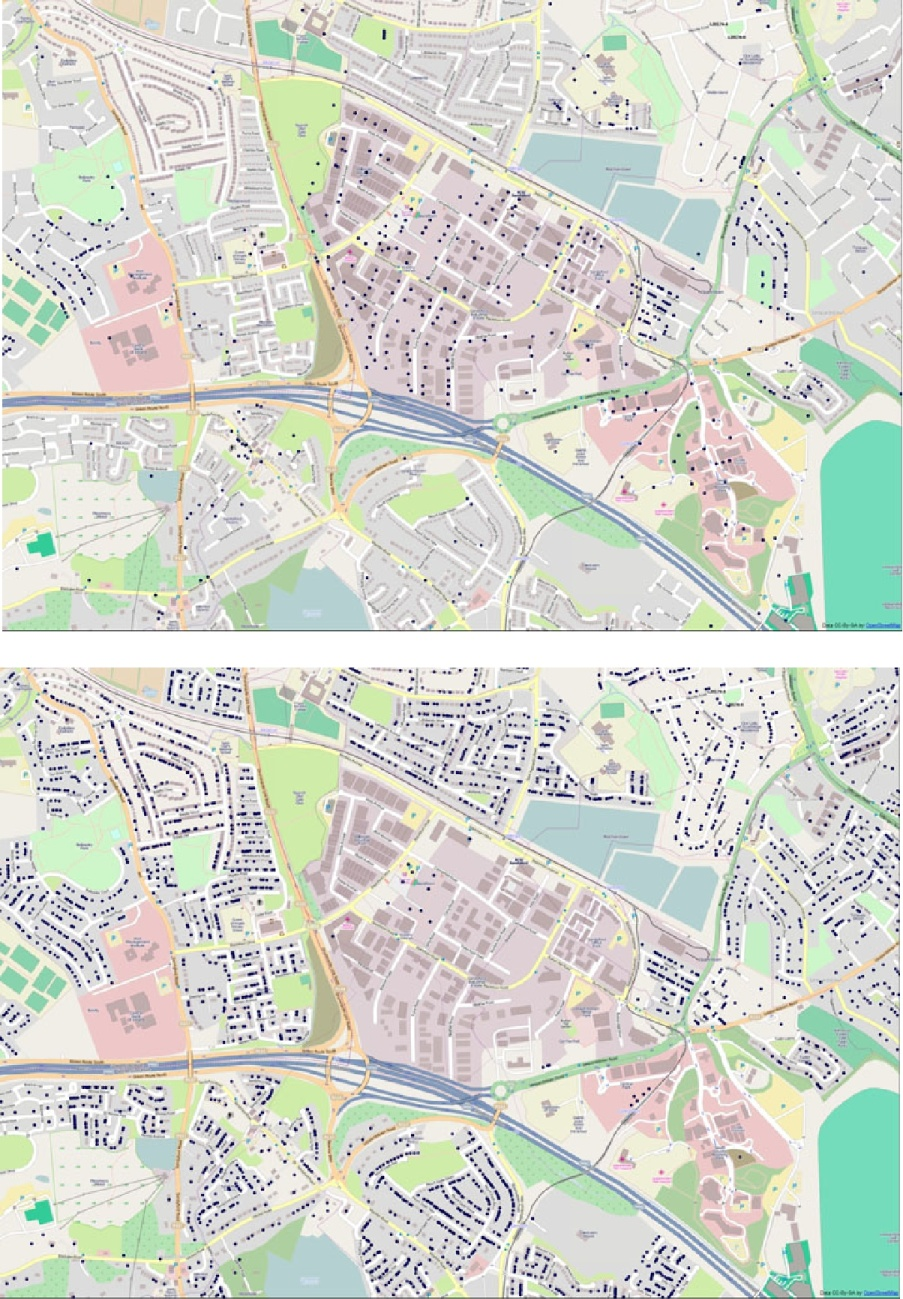
\includegraphics[width=0.99\textwidth, angle=0]{using/figures/dublin0.png}}%
{}
% ------------

% ------------
\createfigure%
{Hourly observed traffic volumes compared to the estimated traffic volumes}%
{Hourly observed traffic volumes (dashed line) compared to the estimated traffic volumes produced by \gls{matsim} using the radiation model (green line) and nearest neighbor model (orange line)}%
{\label{fig:dublin1}}%
{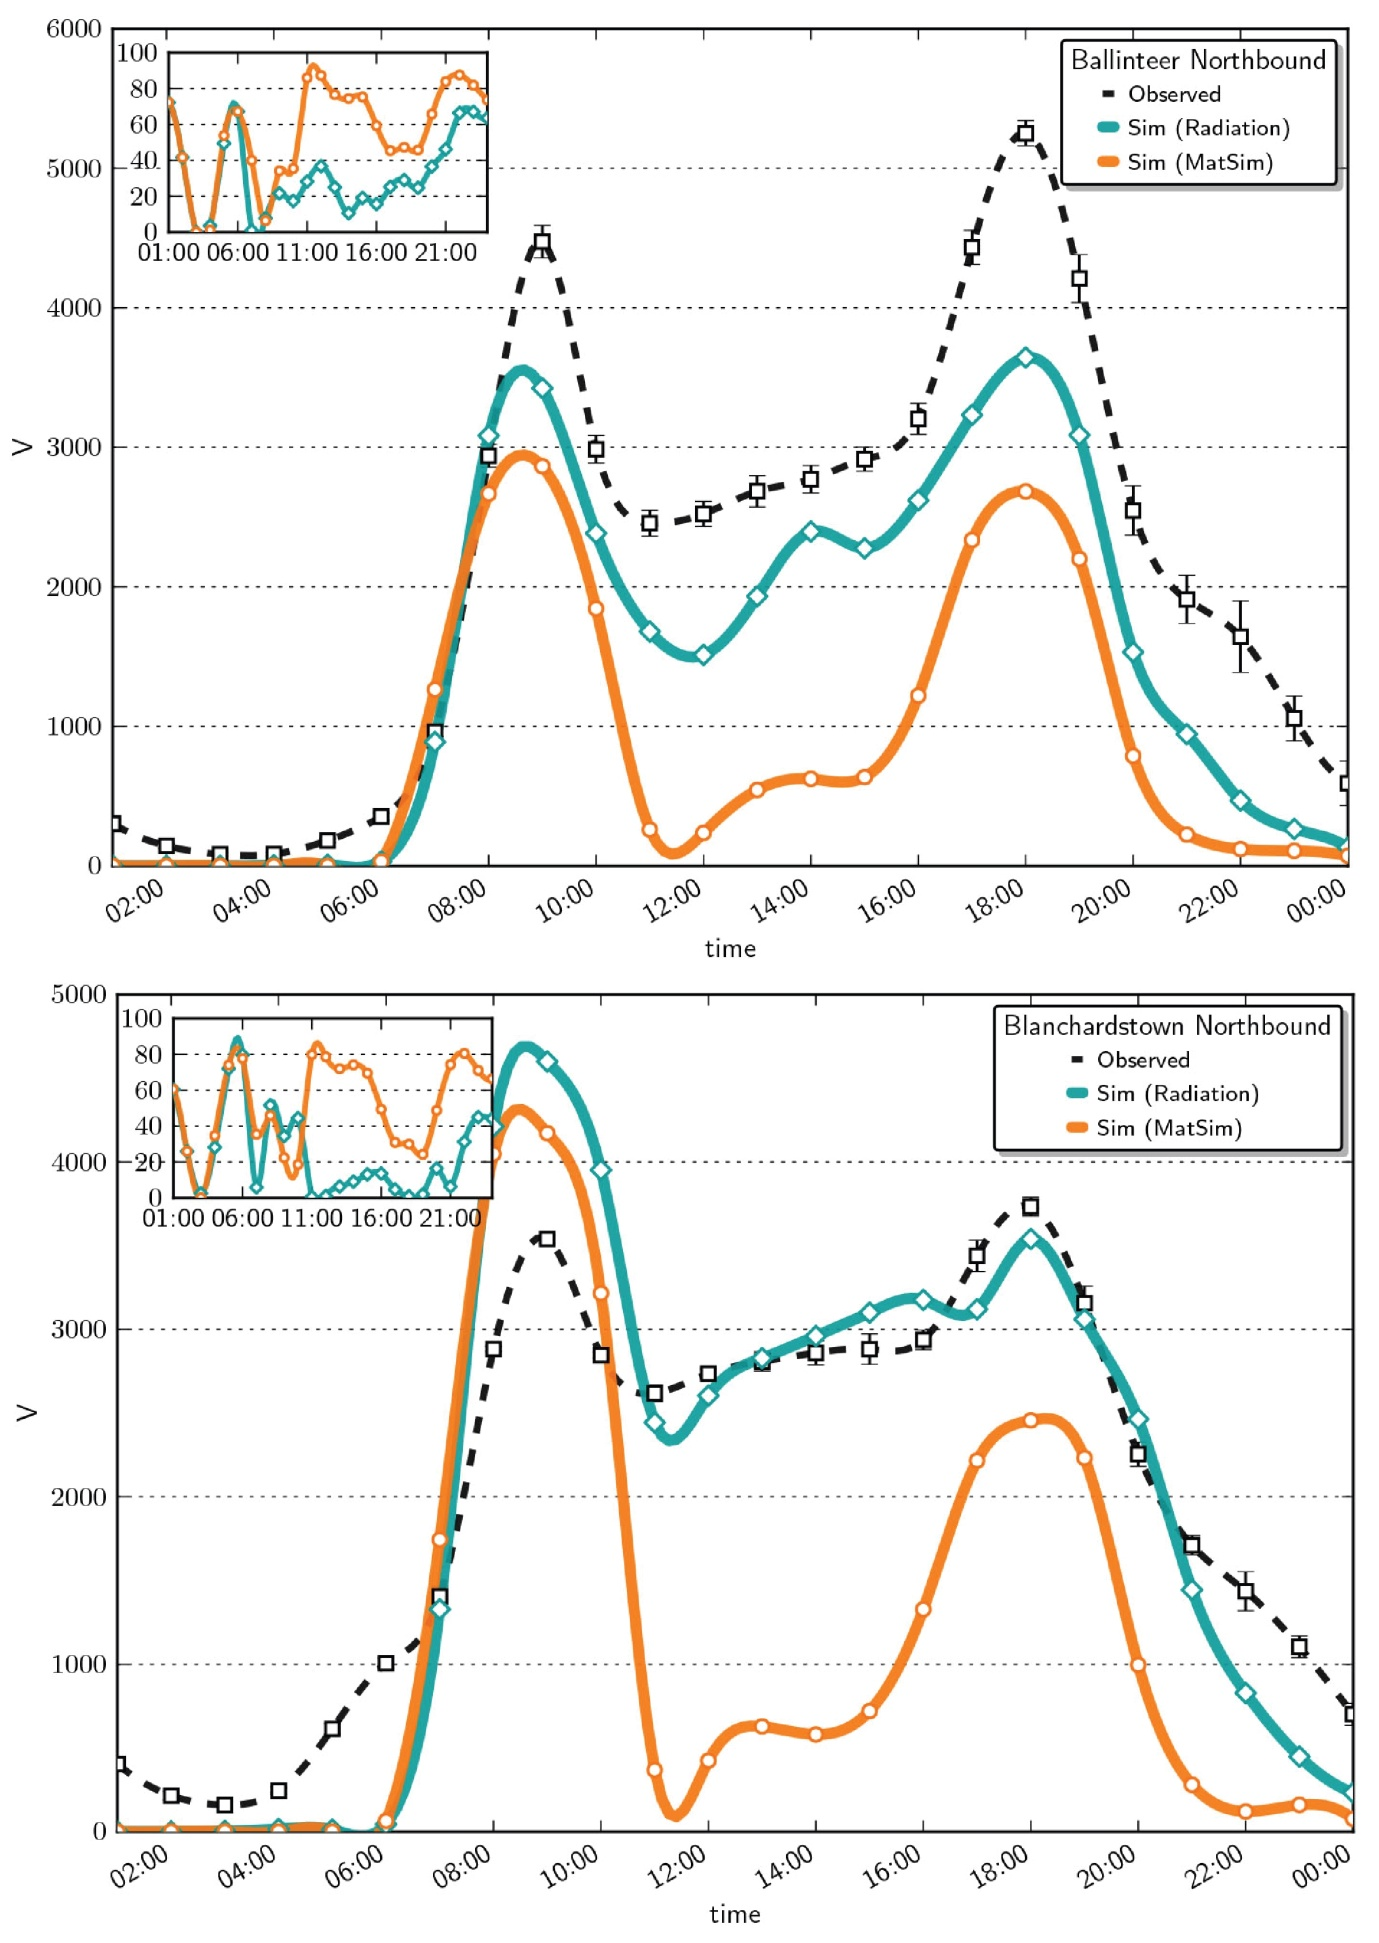
\includegraphics[width=0.99\textwidth, angle=0]{using/figures/dublin1.png}}%
{}
% ------------

% =======================================================================================





 ok

% ==================================================================================================================
% ##################################################################################################################
\section{Gauteng}
\label{sec:gauteng}
\hfill \textbf{Author:} Johan W. Joubert

\editdone{This text has undergone the professional edit. Please no grammatical changes anymore! They are most-probably wrong.}

% ##################################################################################################################
Gauteng is a landlocked province in South Africa, with  three main metropolitan areas: the city of Johannesburg, city of Tshwane (formerly Pretoria) and Eurhuleni. Although the province covers less than 3\,\% of the country's surface, it is the country's economic hub and contributes a third of the country's \gls{gdp}. The 2011~census reported a population of 12.2\,million inhabitants, a quarter of the South African population. 

The first Gauteng scenario was developed in 2008/9 and appeared in \citet[][]{Fourie2009MastersThesis} and \citet[][]{FourieJoubert_SATC_2009}. The population was synthesized from 2001 census data and travel demand was inferred from the 2003 \gls{nhts}. Initially, the network was created from a proprietary source made available for research purposes this has been replaced with a much richer \gls{osm} network.

Early comparisons already showed that the Gauteng \gls{matsim} scenario provided far more detailed results than the four-step models available at the time \citep[][]{Fourie_SATC_2010}. The scenario was also extended to include freight vehicles~\citep[][]{JoubertJEtAl_TRR_2010}.

With the introduction of an open-road tolling scheme referred to as the \gls{gfip}, the scenario was used to study the diversion patterns of different road user groups. The population was extended to included background traffic, in the form of public transport (buses and minibus taxis) and external through-traffic. This data was taken from Saturn \gls{od}-matrices made available by the sponsor, the \gls{sanral}. The impact of the tolling scheme, using vehicle-specific values of time, and a complex toll pricing regime was reported in \citet[][]{NagelKickhoeferJoubert2014HeterogeneousVoTsPROCEDIA}.

The most recent update to the synthetic population generation for the Gauteng scenario is documented on \gls{matsim}'s \url{https://matsim.atlassian.net/wiki/display/MATPUB/South+Africa} Confluence site.

% ##################################################################################################################

% ==================================================================================================================
% ##################################################################################################################
\section{London}
\label{ch:scenarios:london}
\hfill \textbf{Author:} John Serras

% ################################################################################################################## ok

% ==================================================================================================================
% ##################################################################################################################
\section{Los Angeles}
\label{ch:scenarios:losangeles}
\hfill \textbf{Author:} Michael Balmer

% ################################################################################################################## ok

% ==================================================================================================================
% ##################################################################################################################
\chapter{New York City}
\label{ch:nyc}
\hfill \textbf{Author:} Christoph Dobler

\editdone{This text has undergone the professional edit. Please no grammatical changes anymore! They are most-probably wrong.}

% ##################################################################################################################
The \gls{matsim} New York model was an example of an agent-based model based on a given activity-based demand generation process outcome: in this case, the \gls{nybpm} of Parson Brinkerhoff \citep[][]{VovshaEtAl_TRR_2002, ParsonsBrinckerhoff_ResRep_NYBPM_2005, ParsonsBrinckerhoff_ResRep_NYBPM_2009}. It produced persons with individual activity chains; \gls{matsim} was chosen as the simulation-based alternative to conventional assignment processes.

Activity locations were selected on zonal level (3\,824\,zones), timings (\ie start time and duration) were chosen using given distributions. As part of the conversion process to \gls{matsim}, locations were distributed within the zones, according to land use and buildings. For the route assignment, transport modes were converted into those supported by \gls{matsim}. The resulting population contained 5.3\,million persons (25\,\% sample).

A \gls{multimodal} network was created, containing car and public transport links, for the \gls{matsim} model. Car links were derived from the aggregated model network data, including capacity, number of lanes and speed limits. For the public transport network, a shape file containing every lines' routes was available. After converting and cleaning the data, the final \gls{multimodal} network contained 498\,000 nodes and 541\,000 links. Based on further public transport-related data, a full schedule was created, including different public transport modes (bus, train, etc.).

An example for final model outcomes was shown in Figure~\ref{fig:ny_car_share_full} and Figure~\ref{fig:ny_car_share_gross}, depicting the car share of all performed trips within a region. Red indicated a high share, blue a low. In Figure~\ref{fig:ny_car_share_full}, trips were aggregated on zonal level. In Figure~\ref{fig:ny_car_share_gross}, the \gls{matsim} model high resolution was shown; there, the trips were aggregated using hexagons with a side length of 500\,meters instead of a zonal level.

\createfigure%
{Car share (entire modeled area)}%
{Car share (entire modeled area)}%
{\label{fig:ny_car_share_full}}%
{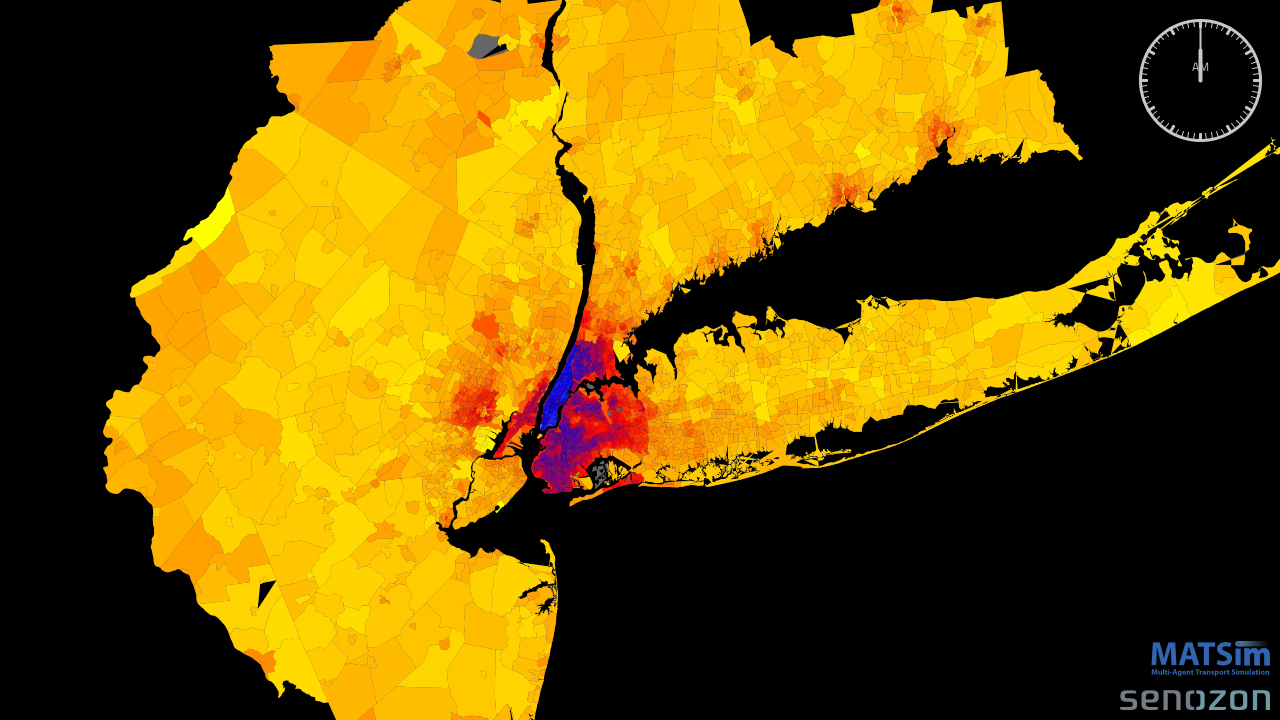
\includegraphics[width=0.95\textwidth, angle=0]{./using/figures/ny_carshare_TAZ_full.png}}%
{}

\createfigure%
{Car share (Manhattan)}%
{Car share (Manhattan)}%
{\label{fig:ny_car_share_gross}}%
{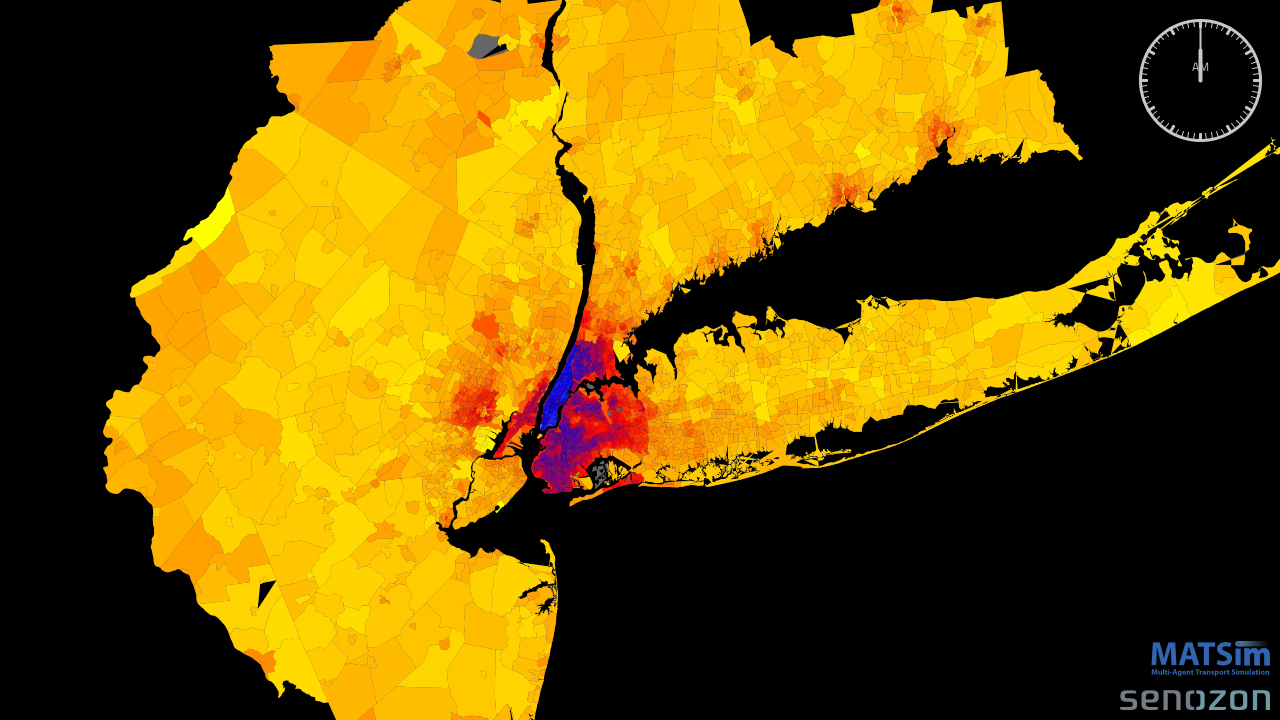
\includegraphics[width=0.95\textwidth, angle=0]{./using/figures/ny_carshare_TAZ_full.png}}%
{}

Finally, Figure~\ref{fig:ny_traffic} showed traffic flows in Lower Manhattan. Cars were represented by rectangulars, public transport vehicles by arrows. Further model outcomes were presented by \citet[][]{Balmer_unpub_ZMNY_2014}. An online movie can be found at \url{http://senozon.com/news/2014-05/zürich-meets-new-york}

\createfigure%
{Traffic flows in Lower Manhattan}%
{Traffic flows in Lower Manhattan}%
{\label{fig:ny_traffic}}%
{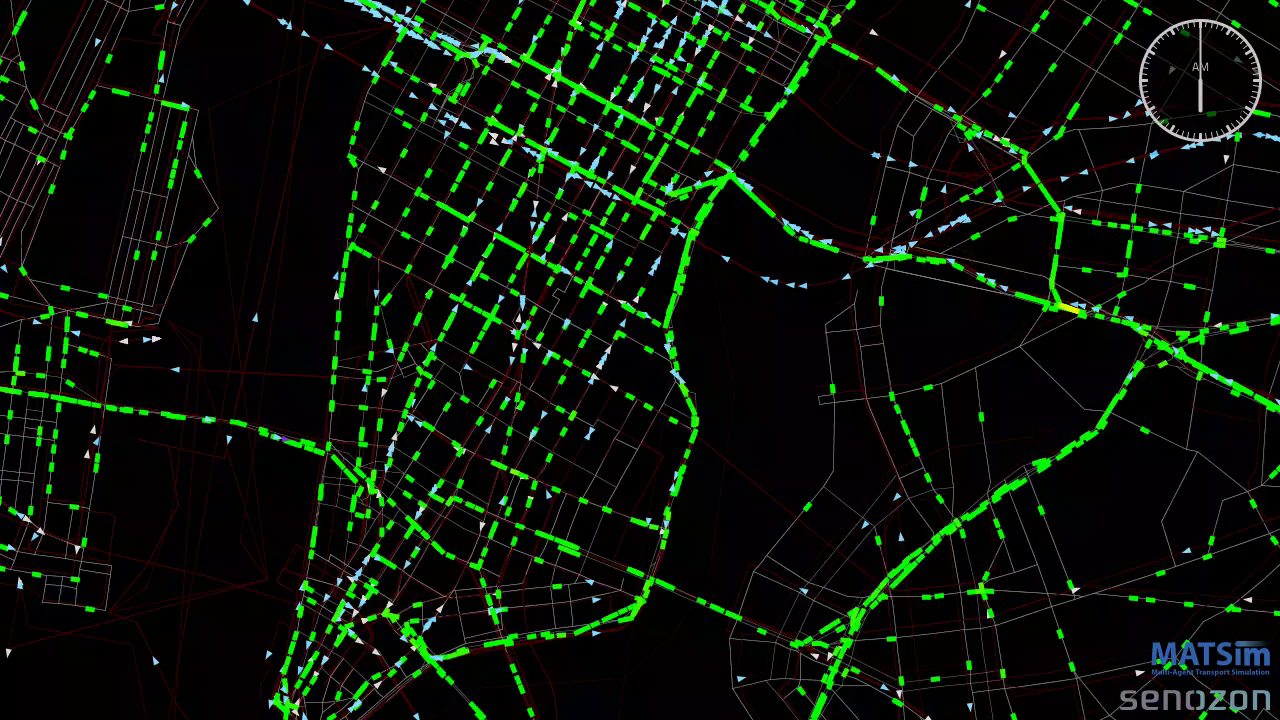
\includegraphics[width=0.95\textwidth, angle=0]{./using/figures/ny_traffic.png}}%
{}

% ################################################################################################################## ok

% ==================================================================================================================
% ##################################################################################################################
\section{Padang}
\label{sec:padang}
\hfill \textbf{Author:} Gregor Lämmel

\editdone{This text has undergone the professional edit. Please no grammatical changes anymore! They are most-probably wrong.}

% ##################################################################################################################
The Padang scenario demonstrated the \gls{matsim} application to large-scale evacuation problems. The scenario was created as part of the third party funded project, "Last-Mile". \citet{00TaubenboeckEtAl2012ConcludingLastMilePaperNatHazards} gives a comprehensive overview.
Padang is located on the west coast of Sumatra Island, Indonesia. In 2014, the city had a population of about 1\,000\,000 people. 
Because of its problematic location on the coast in a so-called "seismically locked" area~\citep{McCloskey2010Padang2009Earthquake}, Padang is prone to earthquakes and subsequent tsunamis. In the "Last-Mile" project, a realistic tsunami scenario, triggered by an earthquake about 300\,km off the coast, was identified~\citep{GosebergSchlurmann2009HazardMappingPadang}. The assumed tsunami would have left about 30\,minutes for the evacuation. The flooding would reach as far as 3\,kilometers inland, thus threatening up to 330\,000 lives. \citet{Laemmel_PhDThesis_2011} developed a \gls{matsim} scenario representing the city with its affected population. One unusual aspect of the Padang situation was the expected universal evacuation by foot; simulating pedestrians with \gls{matsim} was a novelty when this project was undertaken. The standard simulation model (see, e.g., Chapter~\ref{sec:trafficflowmodel}) was thus adapted to deal with pedestrians. 
Details were discussed in \citet{00LaemmelKluepfelNagel2009EvacPadangAtBookTimmermanns}. Another important variation, contrary to most standard transport scenarios, was that network links would flood once the tsunami reached them. Thus, accessibility---flooded or not flooded---of the network links was time-dependent, which was modeled by special time-dependent networks \citep{00LaemmelGretherNagel2009TimeDependentNetworks}. In the time-dependent network concept, link attributes---like \emph{freespeed}---could be changed, while the simulation ran, by precomputed network change events. For the Padang scenario, the network change events were extracted from microscopic flooding simulation data.

% ##################################################################################################################
%
\createfigure%
{Evacuation time analysis for downtown Padang. Numbers showing average evacuation time in minutes, which are also indicated by the colors green, yellow, red.}%
{Evacuation time analysis for downtown Padang. Numbers showing average evacuation time in minutes, which are also indicated by the colors green, yellow, red.}%
{\label{chap:using:padang}}%
{
\includegraphics[width=0.6\textwidth, angle=0]{using/figures/dwntwnpdg}}%
{}

Key Padang scenario facts:
\begin{compactitem}
\item The network consisted of about 6\,000 nodes and 17\,000 links.
\item Synthetic populations for morning, afternoon, and night were created, containing up to 330\,000 agents.
\item The flooding was modeled by a set of 109\,network change events (one per minute), affecting 7\,609 links.
\item A set of 42\,shelter buildings, which could be used for vertical evacuation, was also part of the scenario.
\end{compactitem}
Based on the Padang scenario, various evacuation strategies were investigated:
\begin{compactitem}
\item A seemingly obvious evacuation strategy was the shortest path solution, where everyone is on the shortest path. This solution, however, ignored possible congestion and led to unfeasible results:
\item The Nash equilibrium approach was better, where everyone tried to find an optimal evacuation route through iterative learning \citep{00LaemmelKluepfelNagel2009EvacPadangAtBookTimmermanns};
\item While the Nash equilibrium reduced individual evacuation time, total evacuation time might not have been minimized. The marginal social cost-based simulation approach tried to minimize total evacuation time \citep{00LaemmelFloetteroed2009KISysOptEvac,00DresslerFloetteroedLaemmelNagelSkutella2010OptimalEvacuationLargeScaleScenarios};
\item These three basic evacuation approaches were investigated together with flooding \citep{00LaemmelGretherNagel2009TimeDependentNetworks,Laemmel_PhDThesis_2011};
\item Further, an evacuation strategy to reduce exposure risk was developed by \citep{00LaemmelKluepfelNagel2010PEDRiskPrinted};
\item And finally, \citet{00FloetteroedLaemmel2010ICECShelterEvac} proposed a method to integrate shelter buildings, which are evacuation sinks (i.e.,\,safe places) 
% "\Karen{ What?? sink? Does he mean 'shed', or some kind of building? Or do the buildings have sanitary facilities? Need help with this word.}" 
with limited capacity, into the simulation.  
\end{compactitem}

% ##################################################################################################################


% ==================================================================================================================
% ##################################################################################################################
\section{Patna, India}
\label{ch:scenarios:patna}
\hfill \textbf{Author:} Amit Agarwal

% ##################################################################################################################
Patna is a medium sized city in eastern part of India. Similar to other developing nations, in Patna also, traffic conditions are heterogeneous due to presence of significantly higher number of motorized (motorbike, 14\%) and non-motorized (bike, 33\%) vehicles than car (only 2\%). Therefore, the MATSim queue simulation is modified to simulate travel demand under mixed traffic conditions.

The Patna scenario is created using household survey data from comprehensive mobility plan for Patna \citep[][]{TrippItransVks2009PatnaReport}. To create the Patna scenario, the area under Patna Municipal Corporation is used. The scenario is composed of 72 zones with a population of about 1.57 million (year 2008). In this scenario, MATSim demand is generated using trip diaries. Car, motorbike and bike are used as main congested modes. Passenger car unit for vehicles is derived using effective area occupied by vehicles. In order to allow overtaking of slower vehicles (bike) by faster vehicles (car and motorbike), preexisting, state-of-the-art FIFO (first-in-first-out) queue simulation is overridden using earliest link exit time. Detailed description of the scenario can be found in \citet[][]{AgarwalEtcMixedTraffic}.

Later, the behavior of traffic ow in modified queue simulation is analyzed by plotting fundamental diagrams and space time trajectories for car, motorbike and bike.

% ################################################################################################################## ok

% ==================================================================================================================
% ##################################################################################################################
\section{Poznan}
\label{sec:poznan}
\hfill \textbf{Authors:} Michal Maciejewski, Waldemar Walerjanczyk

% ##################################################################################################################
Poznan, with its population of over 550\,000, is the fifth largest city in Poland, and together with the neighboring suburban area, it makes up an agglomeration inhabited by nearly one million people. The development of the \gls{matsim} scenario for the Poznan agglomeration began in 2012, and since then, the model has been continuously extended and improved. Currently, it is a 24-hour microscopic model of private transport. The goal is to create a 24-hour multi-agent activity-based simulation of the Poznan agglomeration, combining both private and public transport.

The road network model was extracted from \gls{osm} and includes all roads and link roads (such as entrances or exits from motorways). The final result is a high-detail road network model consisting of 17\,026 nodes and 40\,129 links. This model was calibrated in order to determine traffic flow parameters for links (e.g.,\,flow capacity, storage capacity, free-flow speed) for each of the 13\,modeled road classes \citep{PiatkowskiMaciejewski2012osmNetwork}.

The travel demand model was derived from the official trip-based 4-stage model used by the planning department of the city of Poznan; this model dates back to 2000, but since then has been frequently updated. Since the official model was originally designed for the the morning and afternoon peak hours, it had to be extended to describe travel demand throughout the day, hour after hour. As a result, the demand for private transport is represented by 24\,sets of hourly \gls{od} matrices, each set consisting of nine different matrices, one for each of nine travel motivations, namely home $\rightarrow$ work/education/shopping/other, work/education/shopping/other $\rightarrow$ home, and not related to home. This totals up to 216\,\gls{od} matrices \citep{PiatkowskiEtAl2013Poznan24hSimulation, MaciejewskiEtAl2014MikroMakro}.

The official model divides the agglomeration into less than 400\,zones, which is not sufficient for the activity locations to be accurately modeled at the microscopic level. To increase the accuracy, the \gls{osm} land use data were used. Six types of land use, namely residential, industrial, green, commercial, schools and unclassified, were used to subdivide zones into homogenous subzones. As a result, home activities were located in residential subzones, education activities at schools, shopping in residential or commercial subzones, and so on. Figure~\ref{fig:poznan_home_distribution} illustrates the distribution of \emph{home} locations when land use is taken into account \cite{PiatkowskiMaciejewski2013LandUse}.

%---------------------------------------------------------------------
\createfigure%
{Distribution of home activities based on land use}%
{Distribution of home activities based on land use}%
{\label{fig:poznan_home_distribution}}%
{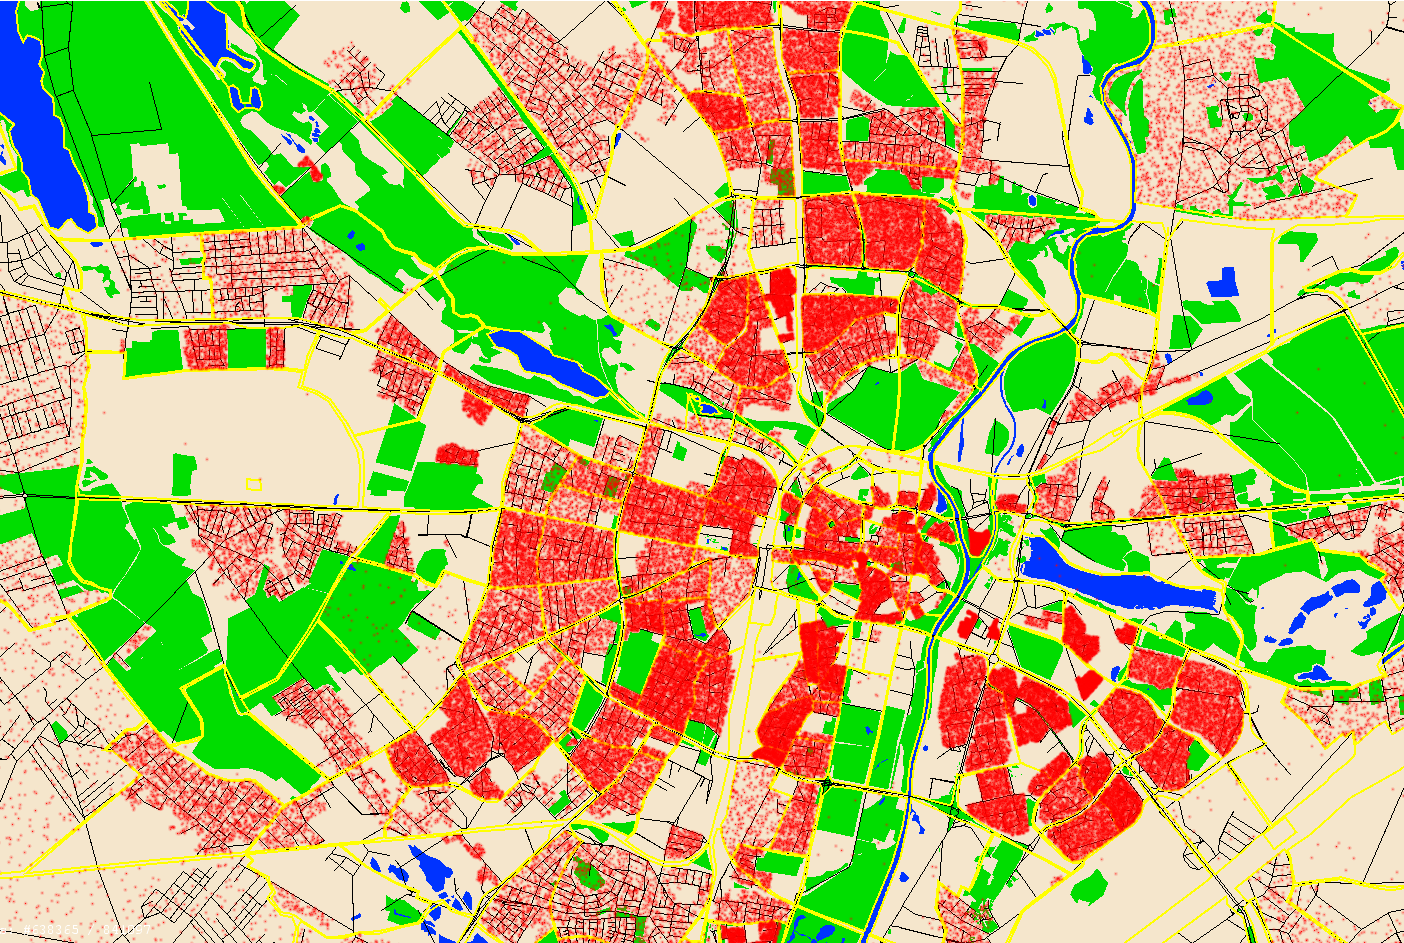
\includegraphics[width=\textwidth, angle=0]{using/figures/poznan_home_distribution}}%
{}%
%---------------------------------------------------------------------

Having calculated the \gls{od} matrices for private transport and subdivided the area into homogenous subzones, the next step was to generate the population of agents. In the first attempt, an assumption was made that each agent performs only one trip, so the number of agents equals the demand represented by the \gls{od} matrices, which is almost 840\,000. Departure times were randomly distributed (uniform distribution) over each hour, and therefore, the only decision made by each agent during the replanning phase concerned the route choice for the preselected pair of locations. The whole simulation consists of 120\,iterations, yet it usually takes about 60\,iterations to achieve a relaxed state. Figure~\ref{fig:poznan_traffic_simulation} shows the state of traffic at 7\,am.

%---------------------------------------------------------------------
\createfigure%
{Road traffic in the Poznan agglomeration at 7\,am}%
{Road traffic in the Poznan agglomeration at 7\,am}%
{\label{fig:poznan_traffic_simulation}}%
{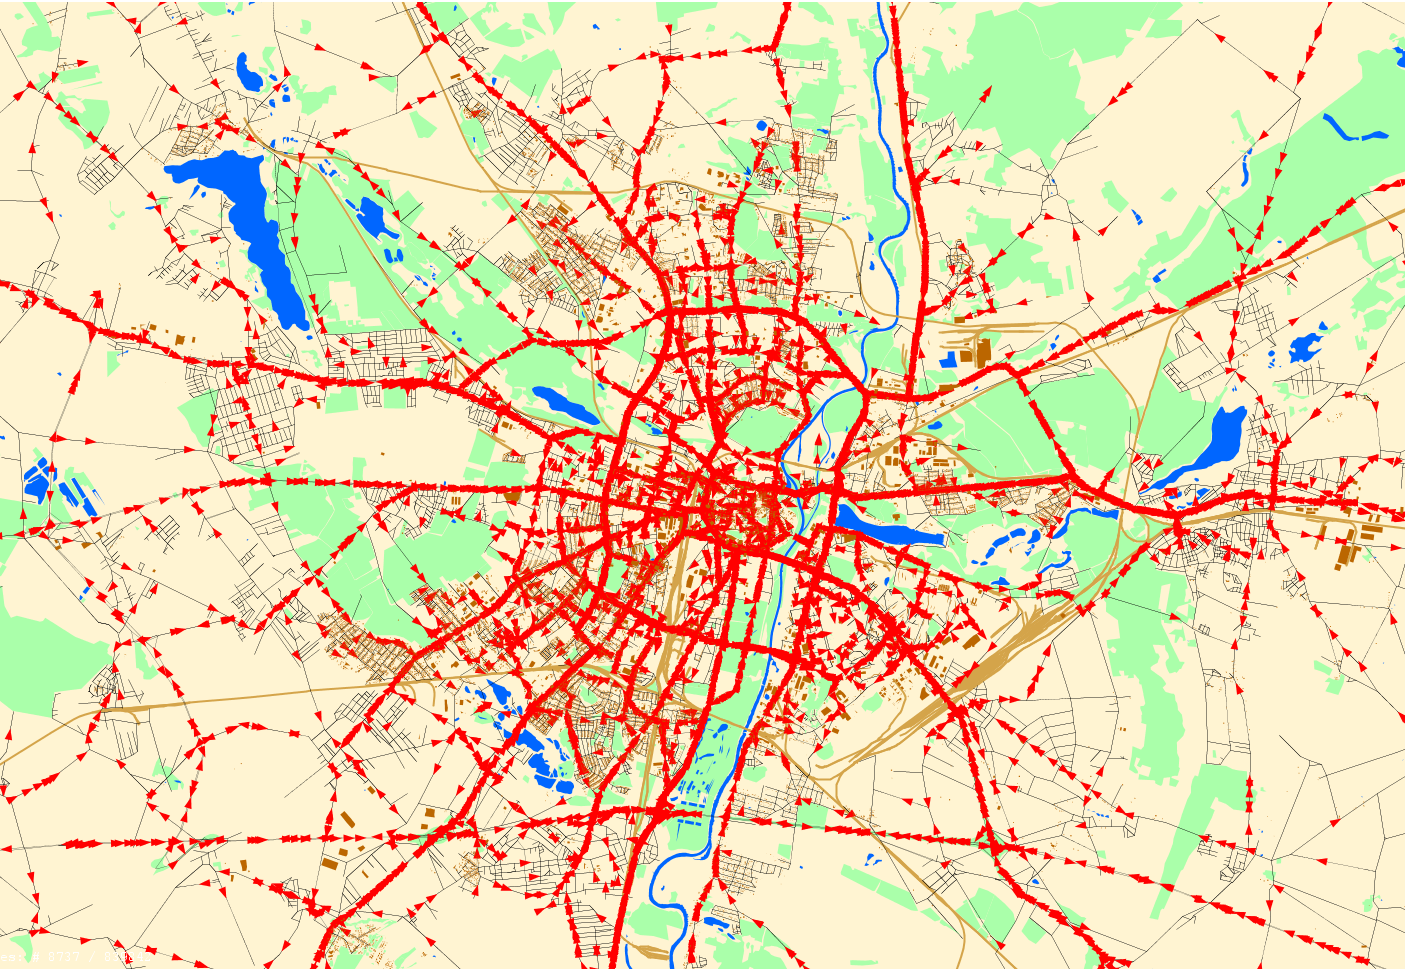
\includegraphics[width=\textwidth, angle=0]{using/figures/poznan_traffic_simulation}}%
{}%
%---------------------------------------------------------------------

Currently, the model is being updated according to a comprehensive travel study carried out in 2014. At the same time, the public transport system is being added, allowing for simulation of both private and public transport. The Poznan model has been used for simulation of real-time electric taxi dispatching, which is done by means of the \gls{dvrp} \gls{extension} (see Chapter~\ref{ch:dts}).

% ##################################################################################################################

% ==================================================================================================================
% ##################################################################################################################
\chapter{Rotterdam: Revenue Management in Public Transportation with Smart-Card Data Enabled Agent-Based Simulations}
\label{ch:rotterdam}
\hfill \textbf{Authors:} Paul Bouman, Milan Lovric

\editdone{This text has undergone the professional edit. Please no grammatical changes anymore! They are most-probably wrong.}

% ##################################################################################################################
In \citet[][]{LovricEtAl_DSS_2013} and \citet[][]{BoumanEtAl_AAMAS_2012}, we proposed two scenarios for studying public transportation revenue management via time-based pricing strategies, like peak markups and off-peak discounts, currently being used by various transit agencies. To evaluate this approach, we developed agent-based simulations using \gls{matsim} and a transportation demand generated from smart-card data collected in a Dutch urban area. In the first scenario, we simulated only a metro network, while in the second scenario we considered a \gls{multimodal} network, consisting of metro, tram and bus.%
\footnote{This research was conducted at Rotterdam School of Management and
supported by Netherlands Organisation for Scientific Research (NWO)
Complexity Grant No. 645.000.001 awarded to Dr. Ting Li and Prof.mr.dr. Peter Vervest from
Rotterdam School of Management. It was presented at \protect\gls{matsim} User Meetings in 2011 and 2012,
INFORMS International 2012 Beijing, the 7th Workshop on Agents in Traffic and Transportation at
AAMAS 2012 Valencia, Erasmus University Rotterdam, Berlin Institute of Technology, Tsinghua
University and Beijing Jiaotong University.}

In \citet[][]{LovricEtAl_DSS_2013}, we designed and implemented a decision support system for sustainable revenue management to evaluate the impact of various revenue management strategies on economic, social, and environmental performance. Figure~\ref{fig:rotterdam} shows the decision support system structure built on top of the \gls{matsim} framework. Smart card transactions (individual check-in and check-out transactions made at stations' entrance and exit gates) were used to reconstruct individual passenger's daily tours. These were inputted into \gls{matsim} as initial demand; information about the transit network and vehicle schedule was extracted from the \gls{osm} data and the public transit operator's web site, respectively. Revenue management experiments were then conducted by applying various time-based pricing strategies defined as percentage-wise discounts or markups (applied on top of the nominal price) during specific periods of the day. 

\gls{matsim}'s loop (Section~\ref{sec:inbrief}) was adapted for studying time-based pricing. First, an event handler was created to calculate whole daily tour travel fare for each individual (this was implemented using the real-life pricing scheme: a fixed fee applied at check-in, plus a variable distance-based fee applied at check-out). Second, we adapted the original Charypar-Nagel scoring function \citep[][]{CharyparNagel2005ga4acts}, by adding travel fare disutility. The existing \gls{matsim}'s time mutator was used as a replanning strategy, allowing passengers to discover more affordable travel times when pricing strategies were enforced (however, a trade-off was introduced by applying a penalty for arriving outside the expected arrival window, based on the observed smart card data check-out times).

To capture revenue management impact on the three sustainability dimensions, we added event handlers to produce a number of relevant \glspl{kpi}. The economic performance was measured by \gls{pto}, passenger kilometers revenue and vehicle load factors. Social performance was measured by seat availability (a proxy for passenger comfort), calculated from vehicle loadings after the mobility simulation. We also looked at average tour price as the measure of public transportation affordability. Impact of a pricing policy on the environment was expressed as the change in carbon footprint occurring through a demand shift between public transportation and private cars (calculated from average tour price change and demand elasticity). 

Our results showed that, by using a smart-card enabled decision support system and taking a customer-centric view, \glspl{pto} can better explore feasible solutions in a broader policy-making context that includes three dimensions of people-profit-planet sustainability. We validated our approach by comparing the simulation-generated travel fares in the nominal scenario with actual fares recorded in the smart card transactional database \citep[see][]{LovricEtAl_DSS_2013}.

To further study smart card data opportunities in demand generation, \citet[][]{BoumanEtAl_AAMAS_2012}, we introduced a pattern-based demand generation method using three different modalities' (metro, tram and bus) smart card transactions in a Netherlands urban area as input. In addition to using single day observations to generate activity-based demand, daily commuting patterns detected from longitudinal observations for a single smart card were generated. In this study, generated demands were utilized to analyze time-shifting behavior under two different revenue management policies: a plain tariff (with a fixed price per journey and a price per unit of traveled distance) and an off-peak discount. The experiment was repeated for different levels of pattern-based demand, where the varied parameter was the number of observed samples required for a smart card to be included. 

In generated demand, agents not generated using pattern-based demand had to replicate their observed tour or trip within 15\,minute windows of observed arrival and departure times. Pattern-based agents had time windows dependent on observed standard deviations in passengers' actual commuting travel patterns, which were used as a proxy for their time flexibility. This aspect of demand modeling was more detailed than \citet[][]{LovricEtAl_DSS_2013}, where agents were assumed to be homogeneous about their time flexibility. This flexibility was exploited by the time shift mutator, made available in \gls{matsim} as one of the \gls{replanning} strategies. In future work, improvements in scoring function and use of more sophisticated pattern-based demand generation approach must be considered to create more realistic scenarios for a study of time-shifting behavior under revenue management policies.

\createfigure%
{Rotterdam scenario}%
{Rotterdam scenario: Decision support system for sustainable revenue management in public transportation}%
{\label{fig:rotterdam}}%
{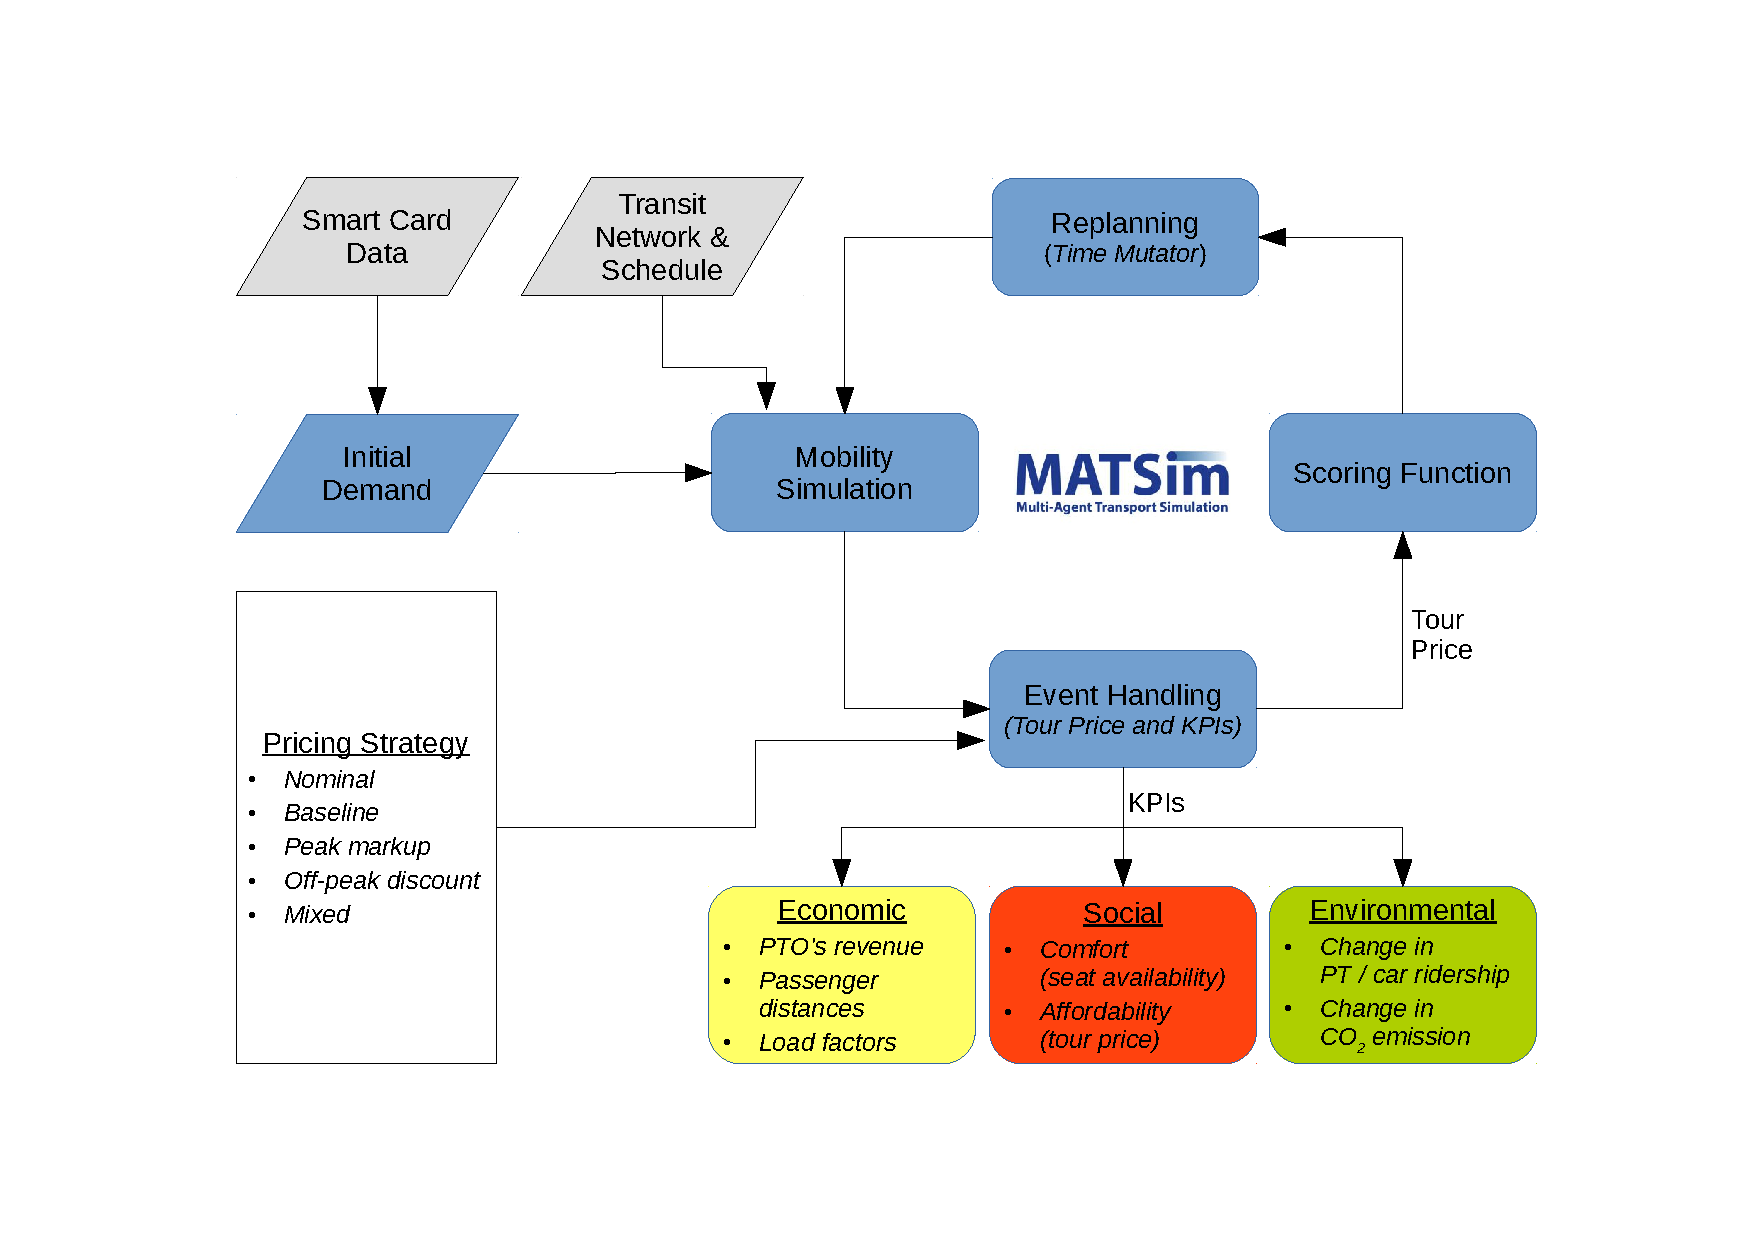
\includegraphics[width=0.85\textwidth, angle=0]{./scenarios/figures/rotterdam}}%
{}

% ##################################################################################################################

 ok

% ==================================================================================================================
% ##################################################################################################################
\section{San Francisco Bay Area}
\label{sec:sf}
\hfill \textbf{Author:} Alexey Pozdnukhov

% ################################################################################################################## ok

% ==================================================================================================================
% ##################################################################################################################
\section{Seoul}
\label{ch:seoul}
\hfill \textbf{Author:} Seungjae Lee, Atizaz Ali

% ##################################################################################################################
The MATSim model of Seoul Metropolitan was developed in 2012 as a result of long-term research collaboration between the University of Seoul (Prof. Seungjae Lee) \& ETH Zurich (Prof. Kay W. Axhausen). The model was updated on a yearly basis and the demand is generated based on 2012 Household Travel Survey Data (HHTSD). The brief statistics related to the demand (input) are summarized as follows. 

The study area covers the Seoul Metropolitan Area (Gyeonggi-do province with emphasis on Seoul Metro which comprises of 25 main administrative districts). Population Synthesizer was developed to generate the MATSim input demand based on HHTS 2012. Total population of SMA is 21.5 million; therefore, a 10\% sample was generated and simulated (2.15 million agents). A detailed network of nodes and links was generated capturing all the details (16'384 nodes and 32'768 links) for railways, highways, arterials, pedestrians, expressways and bus only lanes. EMME/2 network was converted to MATSim format. The 2012 Korean Transport Database was utilized to generate the transit schedules and vehicle definitions according to the bus types, railway and metro lines. Total number of routes is 1'317 (contains regional buses, inter-city buses, feeder line buses and metro lines etc.). In collaboration with Senozon AG, a more realistic door-door demand was generated in Seoul City in July 2014. Data source is the Korean GIS department.

In Seoul context, MATSim has been widely used for various research purposes for policy evaluation, see e.g., \citet[][]{KimEtAl_IJHE_2012, LeeAli_unpub_IWUTSCD_2014}.

A master's thesis is currently underway by this section's second author looking at transit demand generation and calibration using smart card data in SMA. The work is sequenced as follows. A video is available form the authors on request.
%
\begin{compactitem}
\item Data Mining (Trimming off non-useful data)
\item	Converting disaggregate transactions (OD’s )to individual trips and trip segments based on user ID
\item	Activities inference and assignment in SPSS database
\item	Generating transit demand (MATSim input format)
\item	Updated Transit Network \& Schedule for running the simulation
\item	Model calibration (in process)
\end{compactitem}
%
Moreover, MATSim tutorials are prepared for fall semester (2014) to help both undergrad and grad students at the Department of Transportation Engineering in getting working command at MATSim.

\createfigure%
{Seoul Scenario}%
{Seoul Scenario}%
{\label{fig:seoul}}%
{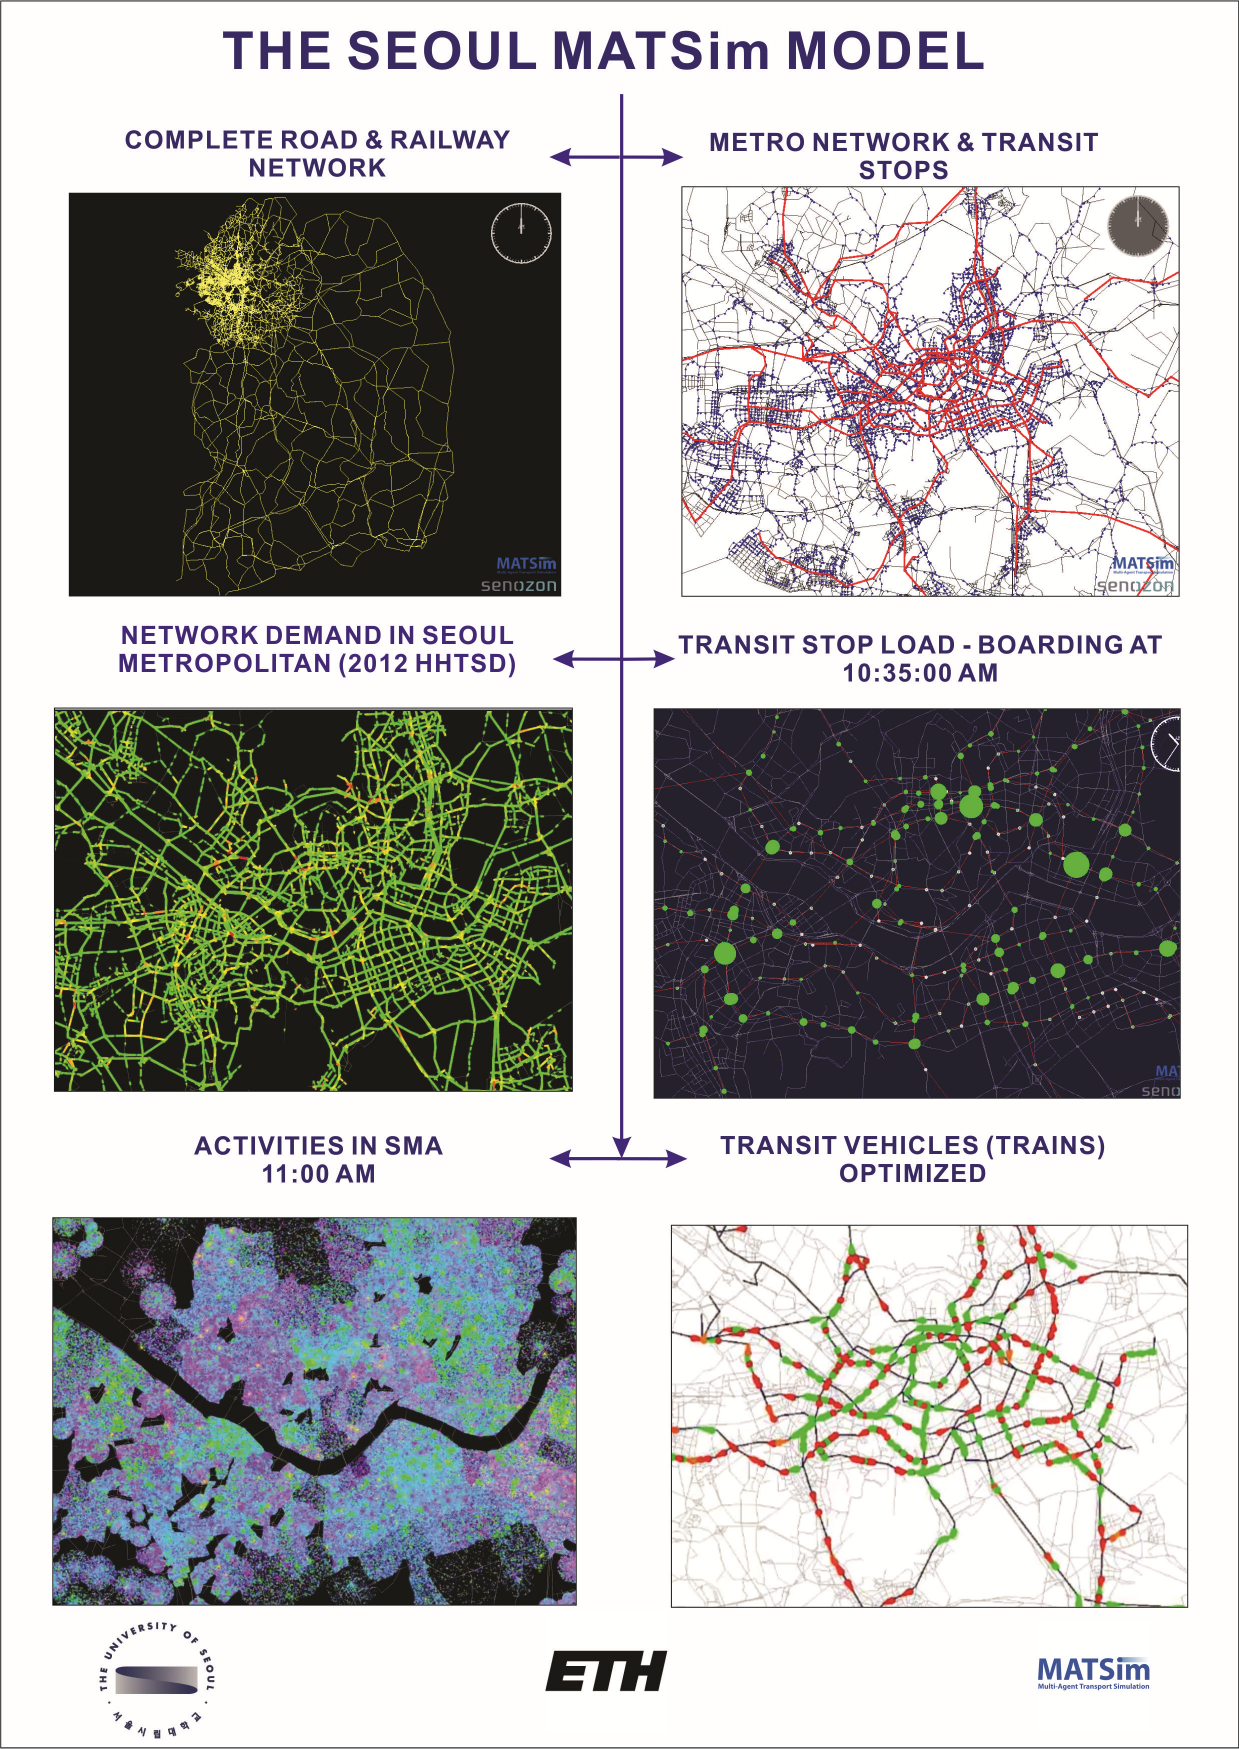
\includegraphics[width=0.99\textwidth, angle=0]{using/figures/seoul}}%
{}

% ##################################################################################################################
 
  ok

% ==================================================================================================================
% ##################################################################################################################
\section{Shanghai}
\label{sec:shanghai}
\hfill \textbf{Author:} Lun Zhang

% ##################################################################################################################
Shanghai, a city of about 20\,million residential population, 6\,073\,square kilometers land area, is the biggest metropolis in China. To fully integrate the activity-based demand modeling and further public transport models, the full implementation of MATSim for Shanghai is built to forecast precise traffic demand on network as well as scientific policy evaluation. The scenario contains 200\,000\,synthetic persons and they are simulated on a network with 50\,000\,links. Key features of Shanghai scenario are as follows.

The 1\,\% sample of the actual population, about 0.2\,million agents, is used. To generate the population individual with personal attributes, MC (Monte Carlo method) are used to disaggregate available census data form the 4th Travel Survey of Residents.

The demand generation is based on 24\,hour OD matrices generated from the GPS data and synthetic population. These OD are then disaggregated into individual trips. The activity-based modeling is used to generate initial population plans by five steps: activity chain choice, duration choice, mode choice, destination choice, and route choice, in which the MNL model is used to estimate and serial choices of agents. During the simulation, activity replanning are still introduced to learn the better travel plans, while scoring for a plan is modeled by using utility-based approach.

The street network of Shanghai has been extracted from the whole OpenStreetMap network and then merged with Shanghai expressway network. Road attributes such as the number of lanes per direction or the flow capacities are set via the specification of road classifications. To simplify the original network, the optimization rules for are designed to remove the useless information that increases the computational burden.

All facilities from OD pairs are classified into the particular zones via their geographical coordinates. Three main facilities types, home, work/education and leisure, are used. The names of origin and destination facilities are obtained via reverse geocoding and these facilities are classified by their names. The resolution of facilities is hectare, in which facilities and types are randomly created according to their coordinates.

Simulated modes are as follows. A public transport system, subways and buses, is integrated with both motor traffic and non-motorized traffic. Whether individuals go to their destination public transits is base on the transit schedules. And a transport mode decision model used to make mode choice by a car or by transit is developed based on the relative utility of travel time of the two modes.

Activity replanning are used to optimize activity plans of agents and the stable state of simulation system is reached after 100\,iterations of replanning procedures. The effectiveness of the Shanghai MATSim transport simulation model is validated against the the observed counts from vehicle detectors and mode split from travel survey. Extensive simulation results indicate that most of the traffic simulation volumes match quite well with the observed counts, and the potential of MATSim for large-scale dynamic transport simulation has been demonstrated. It can provide researchers and policy makers a useful tool to evaluate traffic policies. 

The specific algorithms of integrating new data in Shanghai with MATSim inputs such as synthetic population, facilities and network are separately designed according to data characteristics. To see more detailed work about Shanghai scenario, please see the publications in \citet[][]{ZhangLEtAl_TRR_2014}.

% ################################################################################################################## ok

% ==================================================================================================================
% ##################################################################################################################
\section{Stockholm}
\label{sec:stockholm}
\hfill \textbf{Author:} Joschka Bischoff

% ##################################################################################################################
The Stockholm scenario was created as a student project at TU Berlin in Summer 2014. As several groups worked on the project, the common base are a synthetic population from census data, an OSM based network and counts data.

The network is taken from OSM data in 2013. Within the city, all roads are used, whereas in outlying regions only mayor roads are part of the network.
The demand consists of home-work-home-plans only. The population sample size is, depending on the student group, between one and five percent. Agents are using car and (pseudo) public transit.

Count data for the morning peak along a mayor road, the E4, was used to calibrate the scenario. This calibration was handled differently by the groups; some just added traffic, others tried to imitate the Stockholm toll. Further documentation about the scenario is available in German language. 

% ##################################################################################################################
 ok

% ==================================================================================================================
% ##################################################################################################################
\section{Tampa}
\label{sec:tampa}
\hfill \textbf{Author:} Sashikanth Gurram

% ################################################################################################################## ok

% ==================================================================================================================
% ##################################################################################################################
\chapter{Tel Aviv}
\label{ch:telaviv}
\hfill \textbf{Author:} Christoph Dobler

\editdone{This text has undergone the professional edit. Please no grammatical changes anymore! They are most-probably wrong.}

% ##################################################################################################################
The initial Tel Aviv \gls{matsim} scenario \citep[][]{BekhorEtAl_TRB_2011} was recently extended by adding destination choice to the \gls{matsim} iterations \citep[][]{DoblerEtAl_TechRep_IVT_2014}.

The modeled area was divided into 1\,219\,\gls{taz} (Figure~\ref{fig:TAZ}); geometry was provided as a \gls{esri} shape file \citep{ESRI-ShapeFile_manual_1998}. Zonal attributes contained information on the population living in the zone, as well as types of activities that can be performed.

The population was created using population generator outcomes from the Tel Aviv activity-based model, containing socio-demographic attributes and daily schedules with up to six activities. This kept computational effort manageable; a 10\,\% population sample was simulated. Additional data was provided for external trips; for each of the three types (car, truck, commercial), \gls{od} matrices for three different time periods were available.

Network input data was taken from the \gls{emme2} model \citep[see][]{EMME_Webpage_2015}, also used by the Assignment Unit of the existing Tel Aviv Model. Conversion process details can be found in \citet{GaoWEtAl_TRR_2010}. Turning restrictions were handled by adapting the network structure, resulting in a network containing 9\,474\,nodes and 18\,570\,links (Figure~\ref{fig:network}). Some major road capacities were obviously too low (\eg noticeably lower than traffic counts indicated) and were corrected manually.

The Tel Aviv scenario contained road pricing for two arterial highways; count data for validation was available for three arterial roads.
%\karen{ Why do we have 3 here instead of the word three? I notice it has a \, after it.. is this a special notation?  thanks...}.
%
\createfigure%
{Tel Aviv scenario}%
{Tel Aviv scenario}%
{\label{fig:telavivscenario}}%
{%
  \createsubfigure%
  {\protect\gls{taz}}%
  {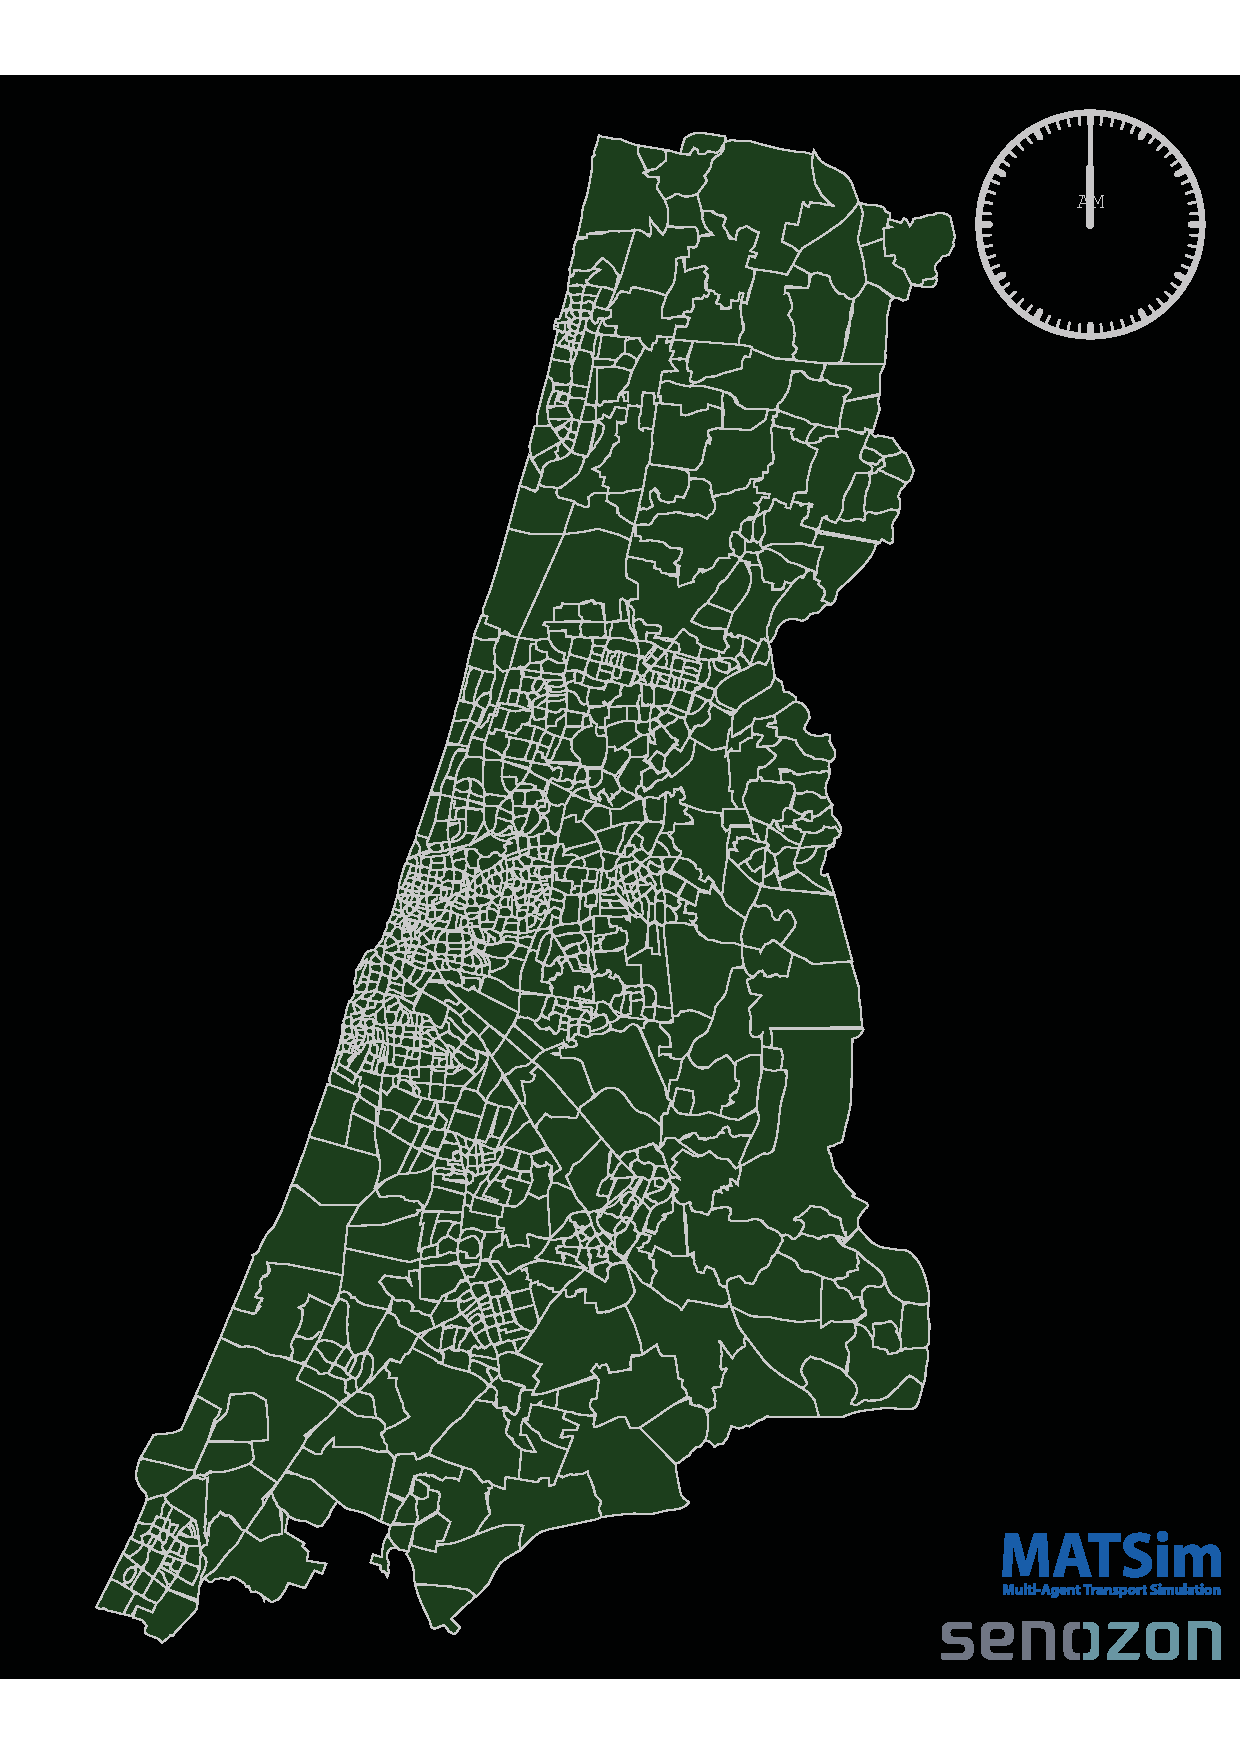
\includegraphics[width=0.49\textwidth,angle=0]{scenarios/figures/TelAviv_TAZ}}%
  {\label{fig:TAZ}}%
  {}%
  \createsubfigure%
  {Network}%
	{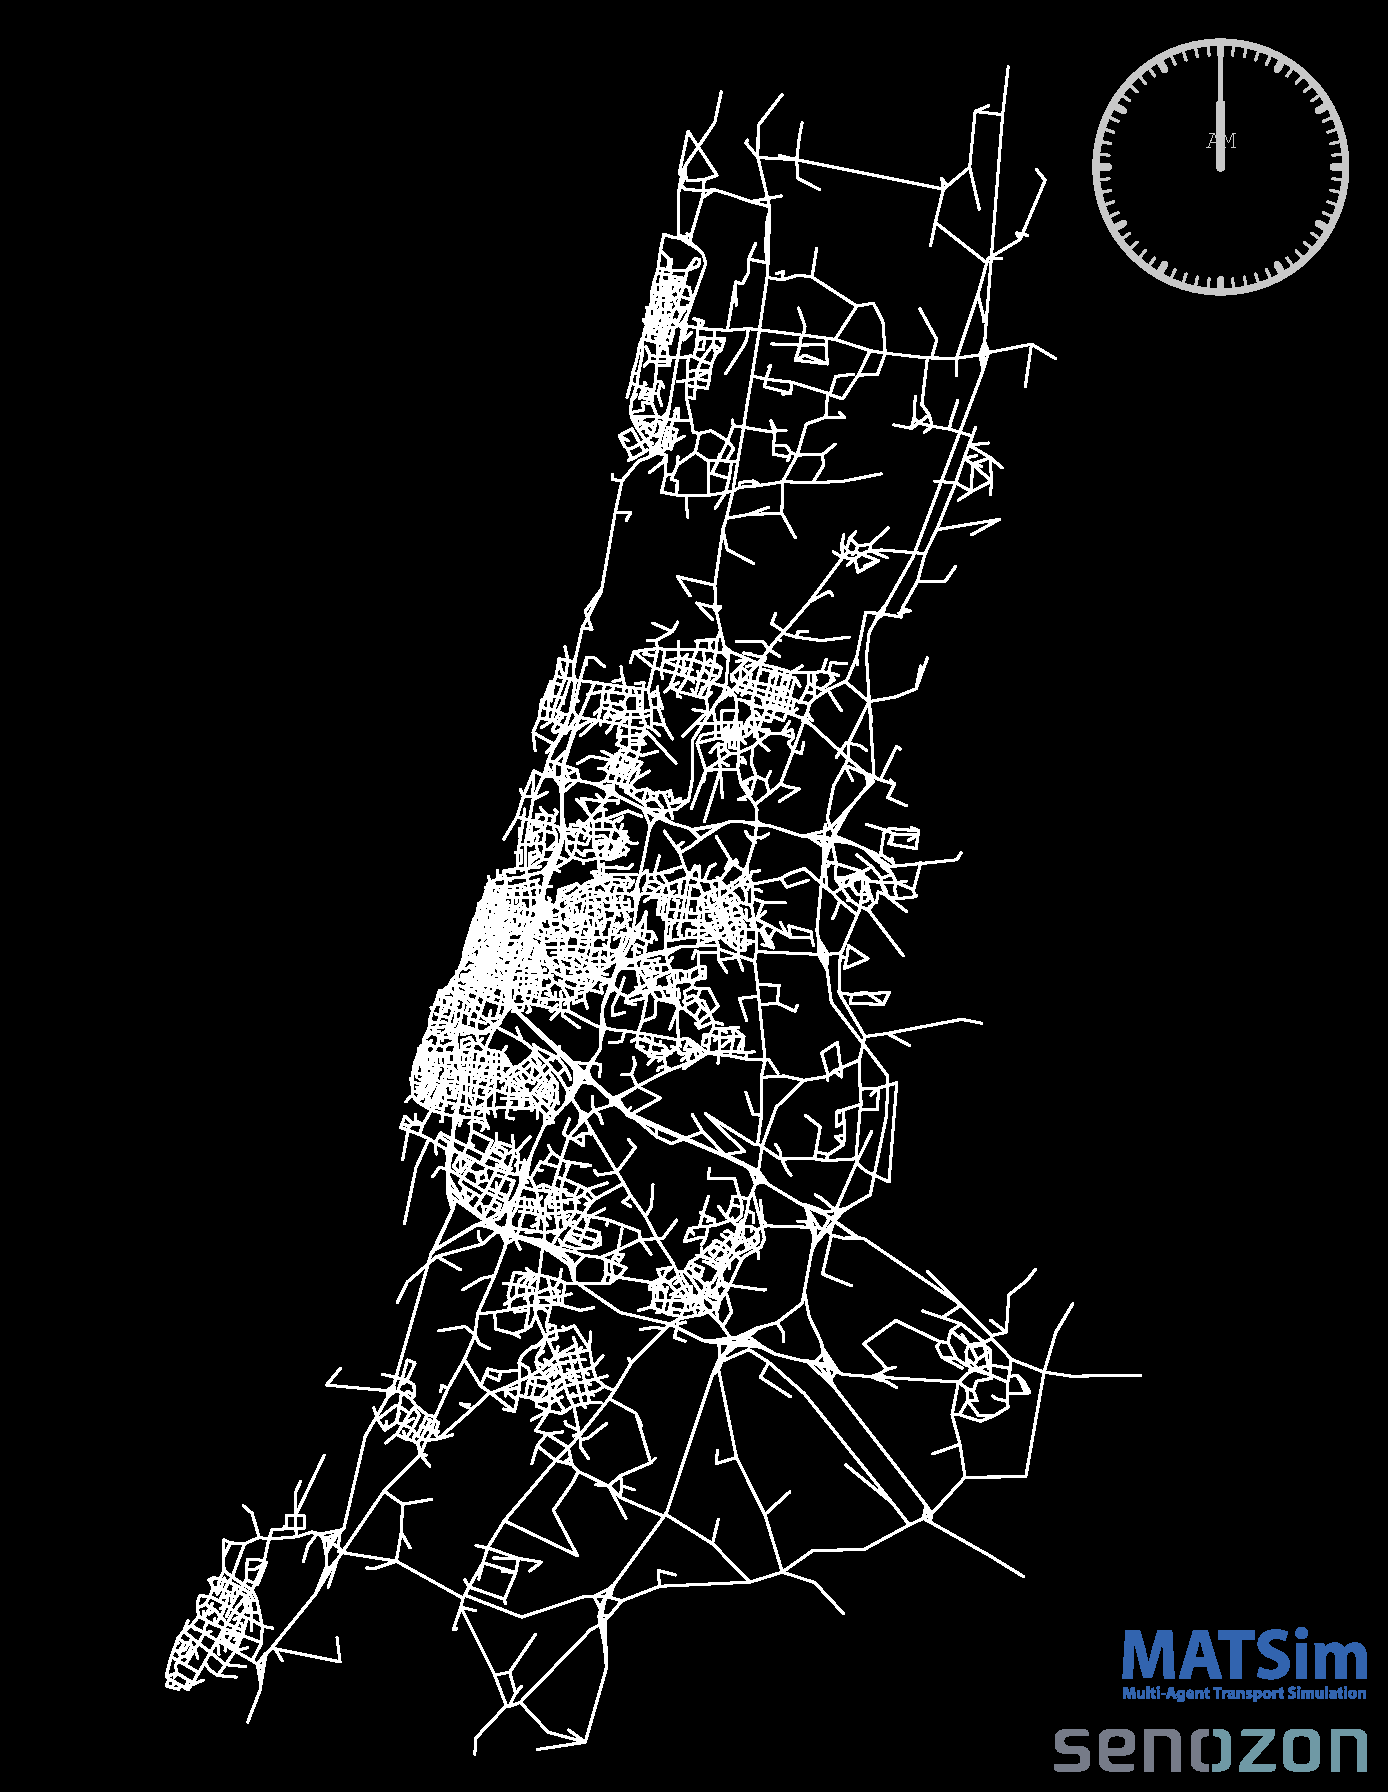
\includegraphics[width=0.49\textwidth,angle=0]{scenarios/figures/TelAviv_RoadNetwork}}%
  {\label{fig:network}}%
  {}%
}%
{}

% ##################################################################################################################
 ok

% ==================================================================================================================
% ##################################################################################################################
\section{Toronto}
\label{sec:toronto}
\hfill \textbf{Author:} Adam Weiss, Peter Kucireck, Khandker Nurul Habib

% ##################################################################################################################
\subsection{Study Area:}
The Greater Toronto and Hamilton Area (GTHA) is situated to the north west of Lake Ontario in the province of Ontario, forming Canada’s largest urban region. The GTHA’s current population is over 6.5 million, with projected growth to approximately 8.6 million by 2031. 

% =============================================================================================
\subsection{Population, Demand Generation and Activity locations}
The Transportation Tomorrow Survey (TTS) forms the basis of the travel demand to be used for the multimodal assignment simulation. The TTS is a retrospective telephone survey conducted in the GTHA every 5 years. The TTS samples just over 5\% of the GTHA households. The survey collects household socioeconomic and geographical characteristics, characteristics of each household member, and a full 24 h travel diary for each household member. The current MATSIM models use the TTS travel diary records to generate the plans file. There has also been some investigation into the integration of the Travel Activity Scheduler for Household Agents (TASHA) activity based model, which has been developed for the GTHA. Irrespective of the source of the demand data, both sources provide the traffic zone location of all activities. The Toronto implementation will then randomly distribute the activities around the traffic zone, resulting in unique x-y coordinates for each activity. Within the current implementation of MATSIM within Toronto, no development of MATSIM facilities has been attempted.

% =============================================================================================
\subsection{Network Development and Simulated Modes}  
The GTHA MATSIM implementation uses a preexisting planning level network for static user equilibrium assignment using the EMME traffic assignment software. This network is converted to a MATSIM network using a conversion tool, which can be found in the MATSIM Toronto playground. More recently, this network was merged with GTFS data for 5 of the 8 major regional transit agencies to allow for multimodal demand assignment.  

% =============================================================================================
\subsection{Calibration, Validation, Results}
The Toronto MATSIM implementation has been compared to the more conventional large-scale assignment models with varying degrees of success. While the work of \citet[][]{GaoWEtAl_TRR_2010}, found that travel time, travel distance, link flows and speeds were all reasonably comparable and in fact more plausible than those achieved through the EMME assignment. Conversely, work on transit assignment done first by \citet[][]{Kucirek_MastersThesis_2012} and then by \citet[][]{WeissEtAl_CJCE_2012} found that there were limitations associated with predicting line boardings based on different transit technologies and agencies, which utilized different fare structure, suggesting that further work to calibrate the multimodal assignment model is required. These issues are exasperated by the current implementations inability to distinguish between in vehicle dwell times and out of vehicle wait times, which ideally should be weighted differently, particularly given the climate and prominence of outdoor bus stops within the region. 

% =============================================================================================

% ################################################################################################################## ok

% ==================================================================================================================
% ##################################################################################################################
\section{Trondheim}
\label{sec:trondheim}
\hfill \textbf{Authors:} Stefan Flügel, Julia Kern, Frederik Bockemühl

\editdone{This text has undergone the professional edit. Please no grammatical changes anymore! They are most-probably wrong.}

% ##################################################################################################################
The Institute of Transport Economics (TØI), in cooperation with Julia Kern from TU-Berlin and Frederik Bockemühl from Hasselts University, built a first prototype model for the region of Trondheim (Norway) \citep[][]{FluegelKern_unpub_WTS_2014}.

The road network data was imported from a publicly accessible data base (Elveg). Figure~\ref{fig:trondheimnetwork} illustrates the network. 
%
\createfigure%
{Network and simulated traffic in Trondheim and surroundings}%
{Network and simulated traffic in Trondheim and surroundings for 6:55\,am \citep[source][]{FluegelEtAl_Samferdsel_2014}}%
{\label{fig:trondheimnetwork}}%
{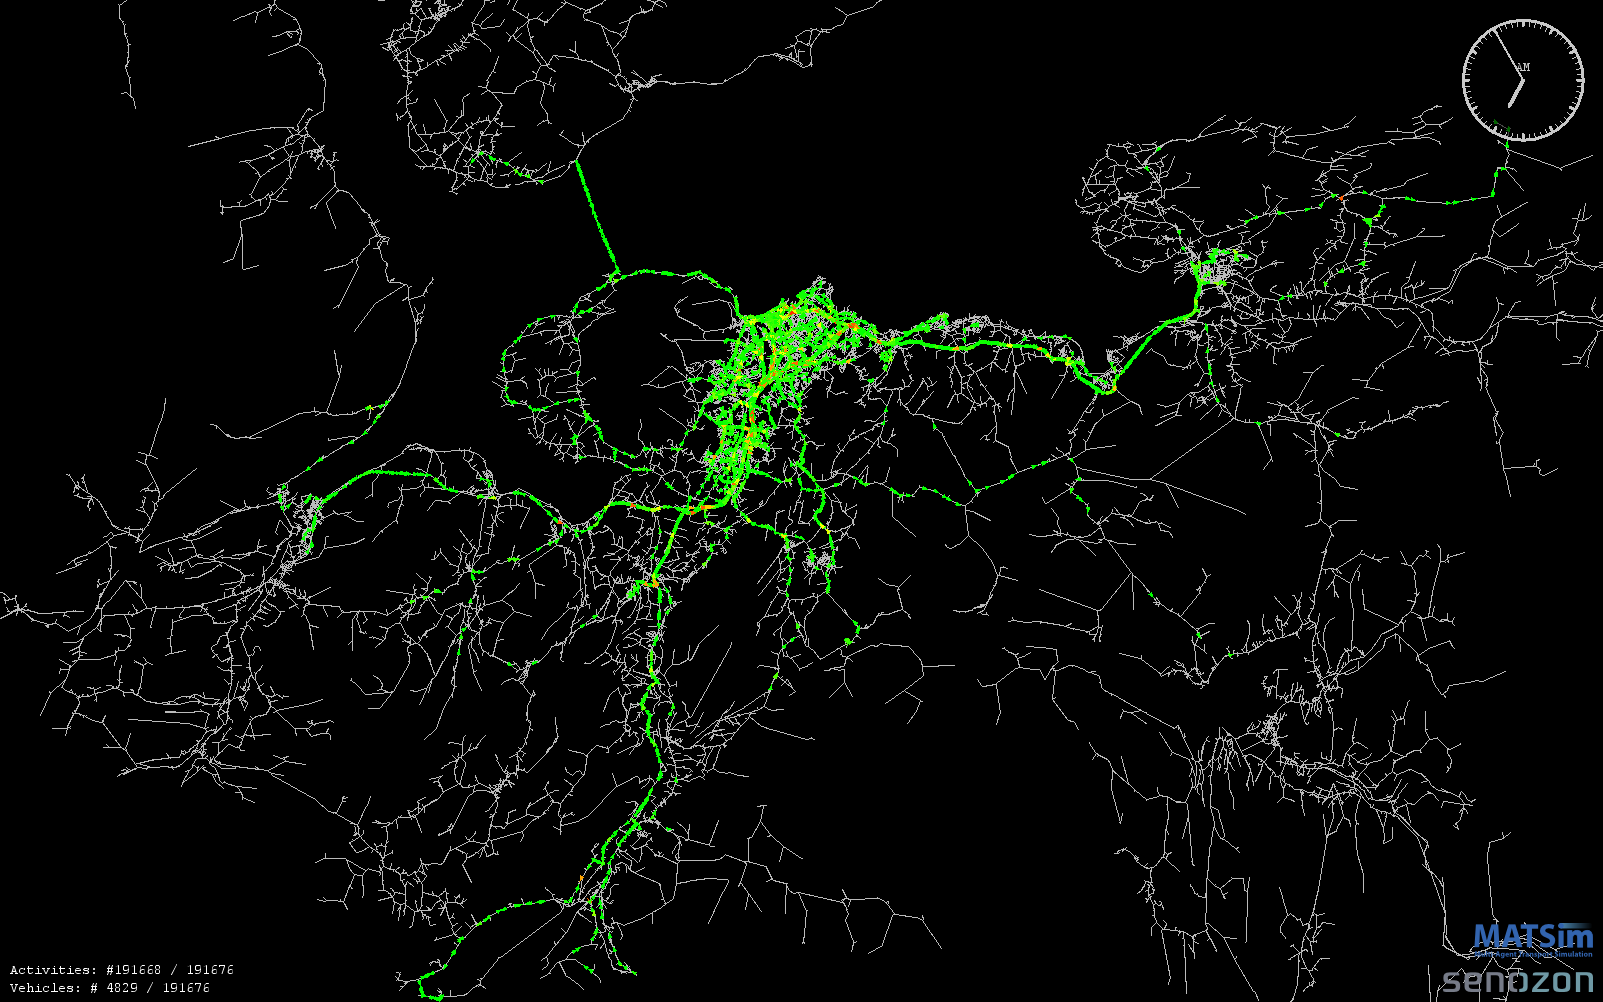
\includegraphics[width=0.85\textwidth, angle=0]{./using/figures/trondheimnetwork.png}}%
{}
%
Most required link information could be directly inferred from the data base. The lane capacity (vehicles per hour) was assumed to be a flat 1\,800 per lane. Existing toll stations, with their current toll structures, were coded manually in the network file. The public transport, walk and cycle networks had not been implemented at this time. Agents using one of these modes were teleported; travel times were calculated with predefined speeds per transport mode. 
Initial demand was derived from the National Travel Survey (NTS 2009) travel diaries. 4\,453 respondents were simply scaled up to 191\,676 agents; activity locations and departure times were slightly randomized to avoid clusters. This model differentiated only between work and ``other'' activities. Desirable working hours were specified as 8\,hours; demand consisted only of private cars (no trucks). 

Standard utility functions were applied, but in the calibration process, default values for travel time disutility in different transport modes were adjusted so that the model would reproduce observed market shares. The simulated traffic fit (in the reference scenario) against real-world counts was deemed satisfactory for a first implementation \citep[][]{Bockemuehl_TechRep_UH_2014}. 

Standard behavioral modules in \gls{matsim} were included in the Trondheim model. Agent could react to policy measures through three choice dimensions: changing route, changing transport mode and changing departure time. To test whether \gls{matsim} predicted reasonable behavioral changes, a small case study was performed. Additional tolls on streets (bridges and tunnels) to Trondheim city center were coded in the network and three congestion price structure were tested. Figure~\ref{fig:loadcurve} illustrates the effects on the simulated cars entering and leaving Trondheim city center. 
%
\createfigure%
{Cars entering/leaving Trondheim city center}%
{Cars entering/leaving Trondheim city center in reference scenario and three congestion pricing scenarios \citep[source][]{Bockemuehl_TechRep_UH_2014}}%
{\label{fig:loadcurve}}%
{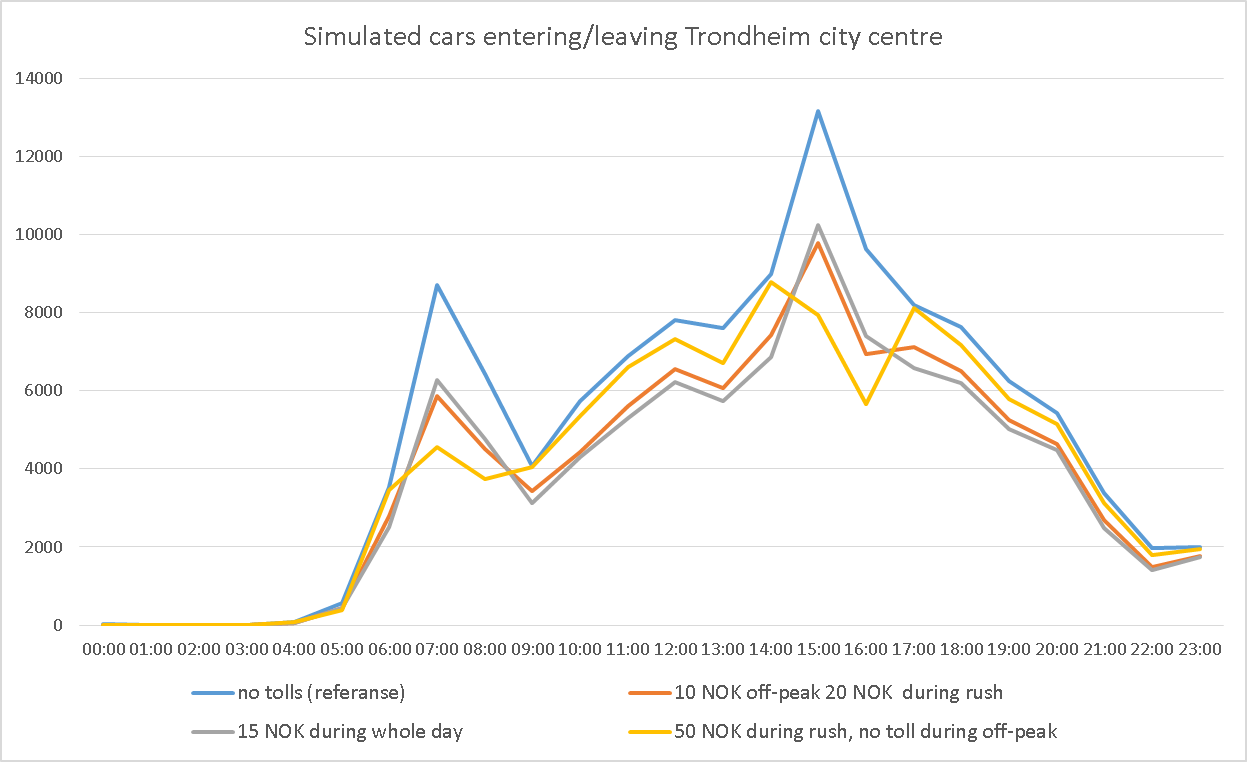
\includegraphics[width=0.85\textwidth, angle=0]{./using/figures/trondheimloadcurve.png}}%
{}
%
Compared to the reference scenario without tolls, total number of cars was reduced in all toll scenarios. Some agents changed transport modes; others, who would have driven through Trondheim center, changed their route. Comparing the three different congestion-pricing structures, it was also evident that agents changed departure time. The difference between the 15\,\glspl{nok} flat scenario and the 10/20\,\glspl{nok} scenario was small; the effect in the 50\,\glspl{nok} rush scenario was substantial. Actually, in this scenario, traffic was heavier before 3\,pm and after 5\,pm implying that many agents changed departure time to avoid high congestion pricing.  

% ##################################################################################################################   










 ok

% ==================================================================================================================
% ==================================================================================================================
\section{2 small towns in regional Victoria (Australia)}
\label{sec:victoria}
\hfill \textbf{Author:} Nicole Ronald


>We've been working with Michal's dvrp module and have had a paper
>accepted at TRB 2015 comparing two dial-a-ride schemes for two small
>towns in regional Victoria, Australia (their current scheme and a
>travel-now scheme). Is that of interest to you for this chapter?
% ==================================================================================================================
 ok

% ==================================================================================================================
Further models are available or currently being developed \citep[][]{Axhausen_unpub_Hong_Kong_2013, MATSIM-T-Scenarios_Webpage_2014}: Rotterdam, Izmir, Aliaga, Caracas.

% ##################################################################################################################
\section{Discussion and TODOs}
Will be commented, when chapter is finished. Make final results traceable.

%\ah{
%- region description (characteristics, stats, ...)
%- population (popgen, Balmi plug together)
%- facilities
%- network
%- utility function (estimated, how derived)
%- pt (simulated, pseudo pt)
%- modes
%- freight (siehe keynotes Kai)
%- border crossers/boundary effects
%
%data sources
%methods applied
%
%- special problems faced \& solutions found
%
%- simulation quality
%- calibration \& validation (+available data)
%
%- purpose and sponsor/client
%- associated projects -> see Section \ref{sec:projects}
%
%- specialties: parataxis in Gauteng, connections to other sims (Toronto, Tel-Aviv)
%}

\ah{
Rotterdam (Milan Lovric->message failed, Bouman): angefragt

the Netherlands (coupled with Albtratross (by whom? Dobi?),

Chicago? -> Wiepersdorf
}

% ##################################################################################################################
 \cleardoublepage

% core MATSim mit Core (Default-) Moduls
% -----------------------
\part{Extending MATSim} \cleardoublepage
\chapter{Modules: Configuring and Extending MATSim Functionality}
\label{ch:modules}
% ##################################################################################################################
% ##################################################################################################################

\hfill \textbf{Author:} Andreas Horni

\begin{center} 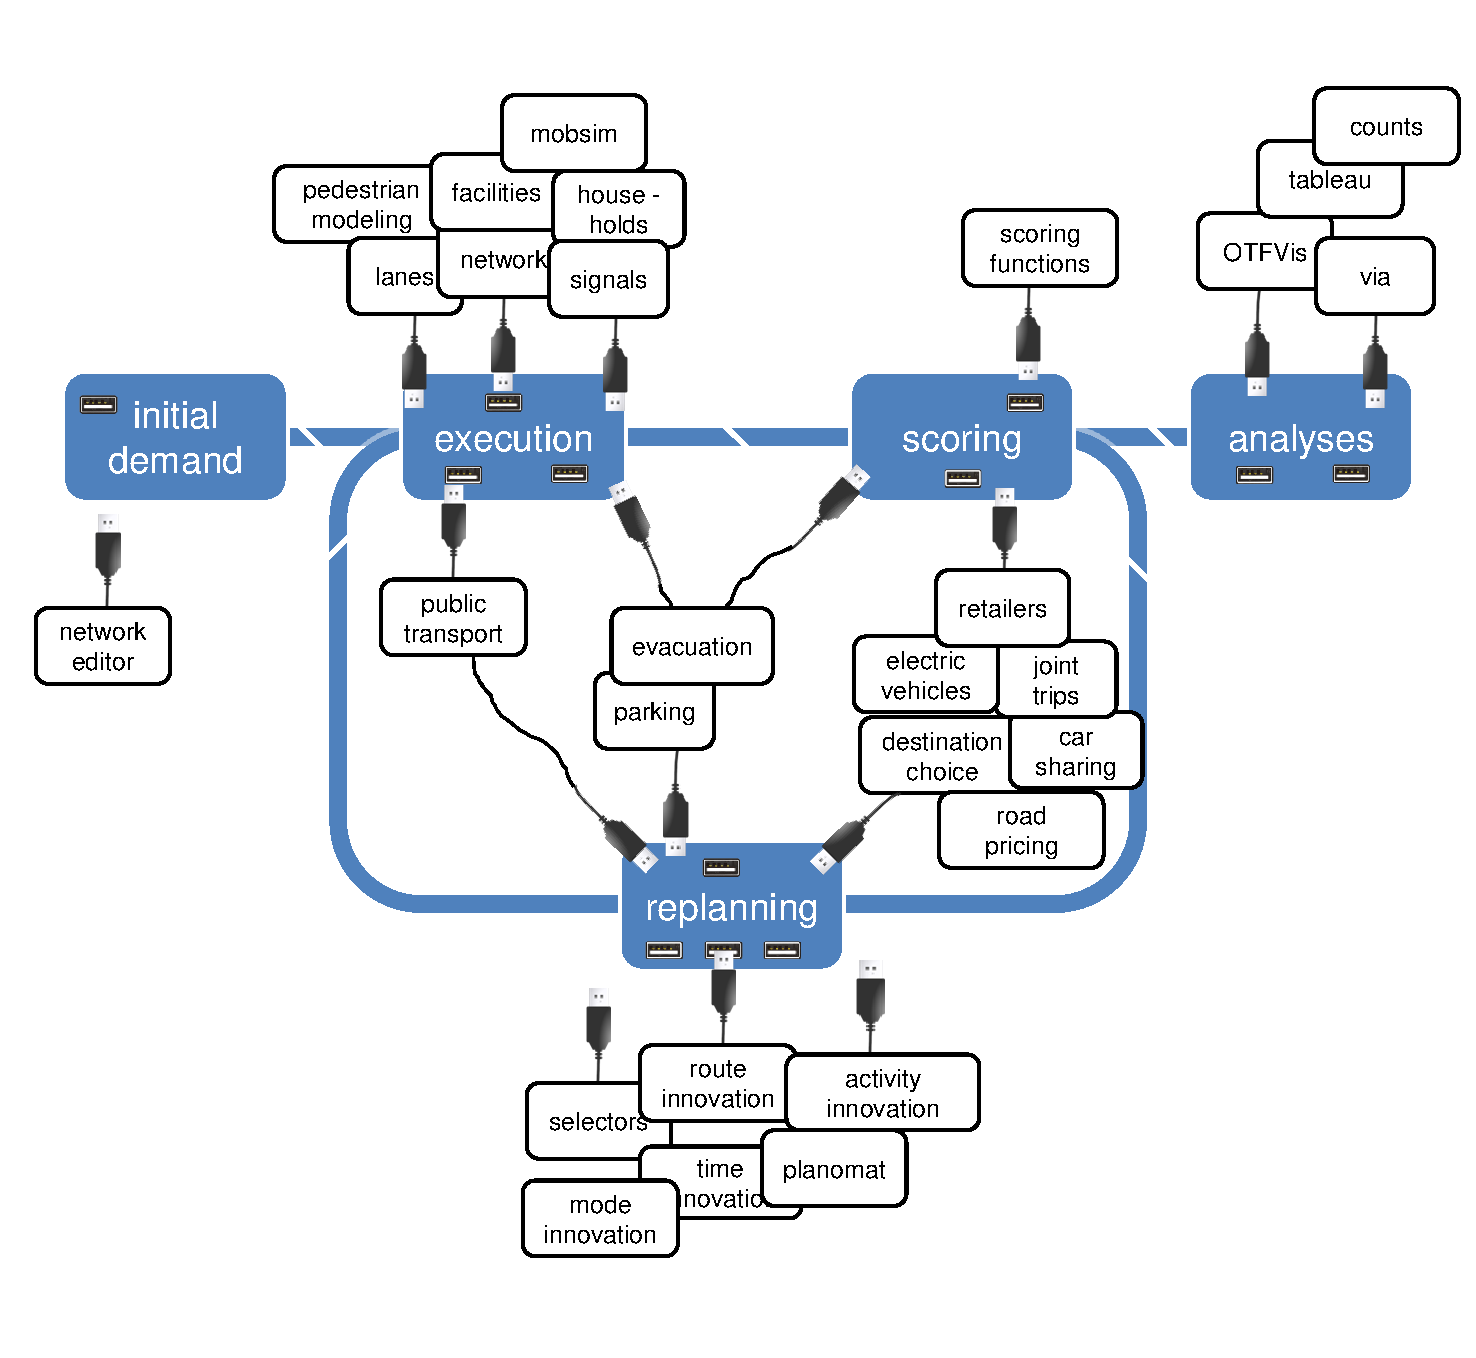
\includegraphics[width=0.5\textwidth, angle=0]{extending/figures/modules.pdf} \end{center}

% ##################################################################################################################
\section{Modules}
Due to its modular design MATSim is a highly flexible framework. As shown in Section \ref{sec:usingmatsim}, it can thus be configured and extended in various ways. When it comes to configuring MATSim the term ``module'' is very extensively used. Due to the danger of ambiguity, this consequence of organic grows needs to be corrected on the long run, for now, we try to just sort out the different meanings of the word module.

The term ``module'' is used for components providing distinct functionality, residing in the \lstinline|org.matsim| package and having their own section in the default configuration file. Such a section looks as follows. 
\begin{lstlisting}
<module name="aModule"> 
    <param name="aParameterForAModule0" value="someValueX" /> 
    <param name="aParameterForAModule1" value="someValueY" />  
</module>
\end{lstlisting}

The term ``module is furthermore used for contributions, residing in the \lstinline|org.matsim.contrib| package and either having their section in the default configuration file (such as destination choice) or not (such as the wagonsim contribution). 

Also external components plugged in and replacing a MATSim module, such as a mobsim, are called modules.

Also the standalone tools referencing MATSim as a library, such as the network editor, or the visualizer via, are termed modules in current practice.

A slightly different meaning of modules, which is only relevant for the MATSim developer and API-user, is as follows. In the package package \lstinline|org.matsim.core.replanning.modules| replanning functionality is provided in classes that are derived from \lstinline|AbstractMultithreadedModule|. The majority of these modules have their own section in the configuration file, but some do not, such as the \lstinline|TripsToLegsModule|. In that package---called modules---there are furthermore, the factories for the plan selectors. For the selectors and their factories, it is unclear if they are modules too.

To make things worse, there are cases where module names in the configuration file are not (yet) consistent with the naming in the code. Examples are ``\lstinline|strategy|'' in the configuration file and ``\lstinline|StrategyManager|'' in the code, or ``strategy module'' in the config file and ``\lstinline|PlanStrategy|'' in the code \ah{Nochmals nachsehen!}. Furthermore, modules are atomic. There is, for example, a module called ``\lstinline|ChangeSingleLegMod|'', a module ``\lstinline|ChangeLegMode|'' and a module ``\lstinline|SubtourModeChoic|'' instead of one single module called ``\lstinline|ModeChoice|''. This, on the one hand, has historical reasons; the three modules were developed temporally separated. On the other hand, the parameter set for a module is only minimal and unambiguous if provided for atomic modules as different parameters are required for the three modules.

For the presentation of the available functionality, we chose to not use a single section per module but to group them according to common transport planning categories, in the example above this would be ``mode choice'' instead of the atomic categories, where we use terms ``functionality'' for the larger categories and ``module'' for the atomic components. 

MATSim currently offers the functionality depicted in Figure \ref{fig:matsimmodules}. The figure shows where in the MATSim loop, the functionality can be plugged in. The technical details for their usage, in particular the parameter sets are described in \citep[][]{MATSim_Userguide_2014}.

\createfigure%
{MATSim functionality}%
{MATSim functionality}%
{\label{fig:matsimmodules}}%
{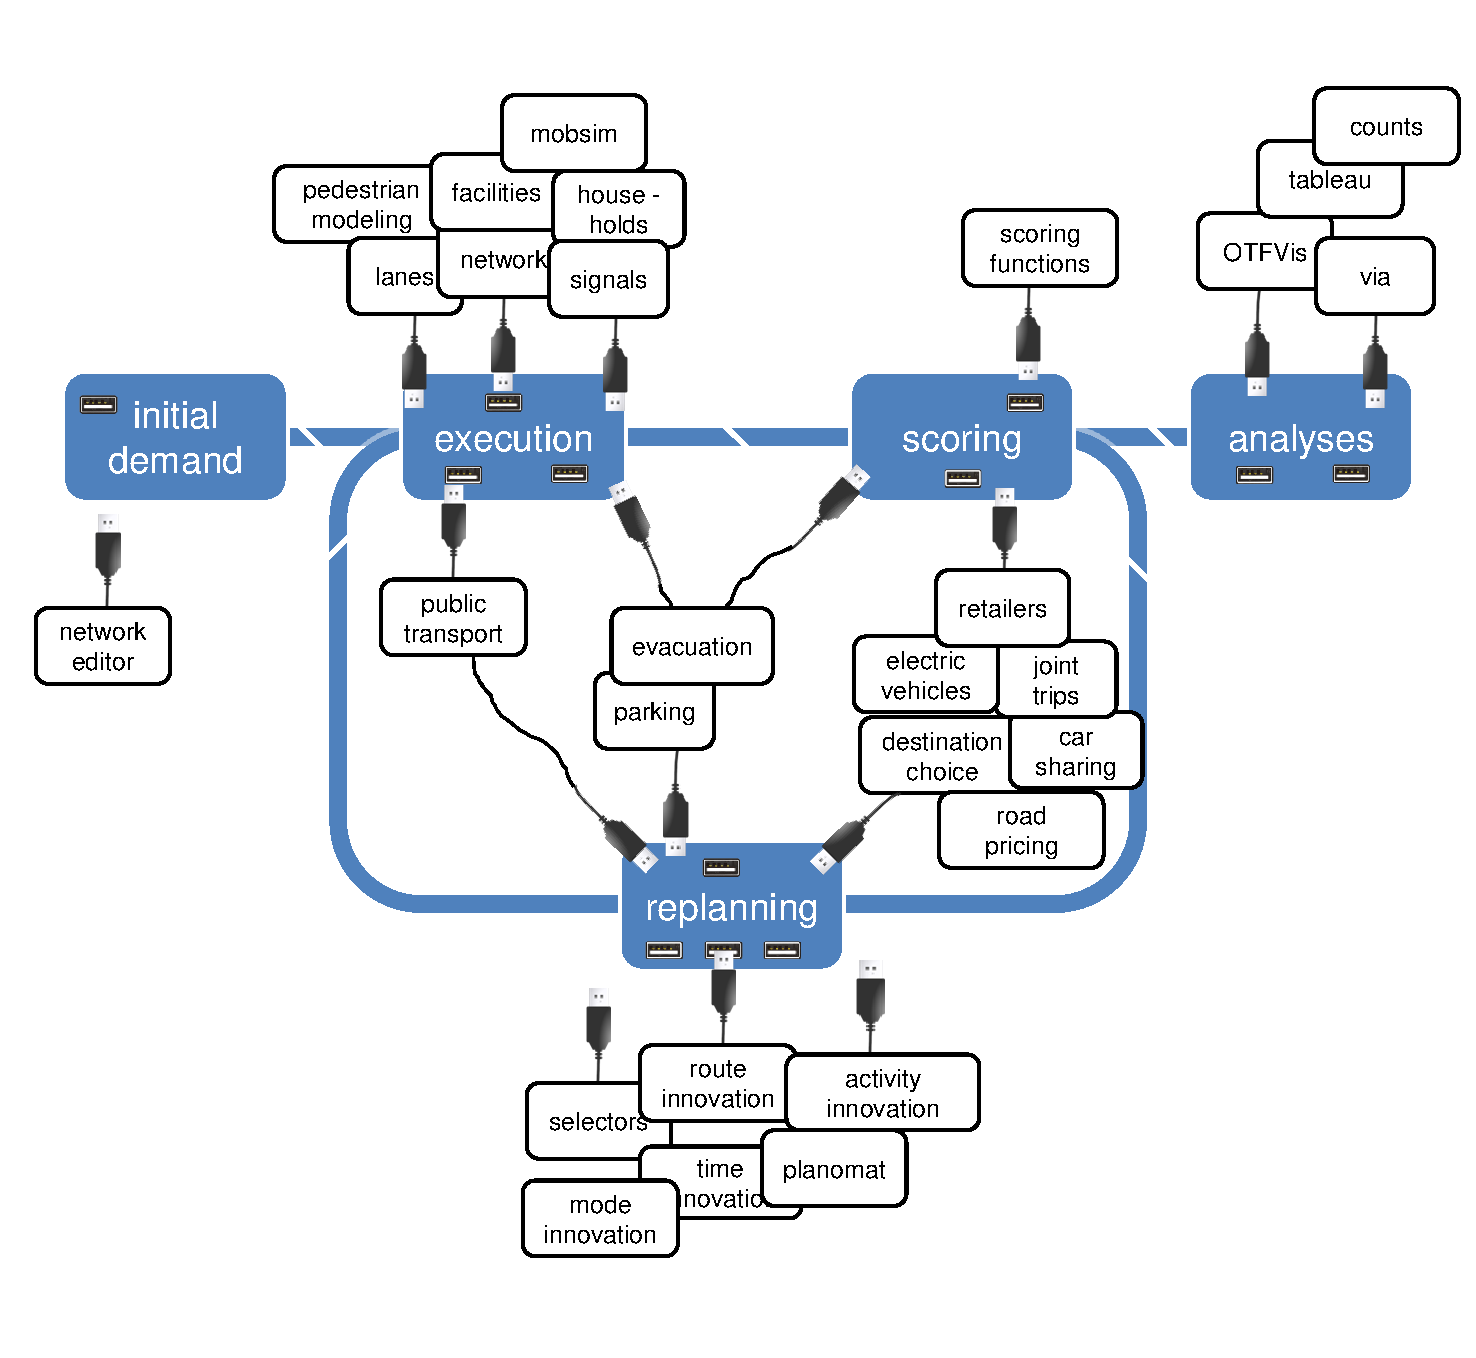
\includegraphics[width=0.99\textwidth, angle=0]{extending/figures/modules.pdf}}%
{}

Due to the distributed and project- and dissertation-driven MATSim contribution process (see Chapter \ref{ch:developmentprocess} modules are usually implemented for a specific practical purpose leading to various limitations of the respective module, e.g., modules might only work for a specific mode or for a defined calling order. Before, an additional effort is undertaken to generalize the module toward its embedding in the complete framework, the combination of a specific module with other functionality remains a non-straight-forward task. This means, that the user is in charge of systematically testing a specific modules combination before productively applying it.

MATSim provides the possibility that the parameters of arbitrary external modules are added to the configuration file as shown above. In the respective module, the parameters can be accessed with the method \lstinline|public final String findParam(final String moduleName, final String paramName)| of the \lstinline|Config| class.

% ##################################################################################################################

\ah{Einteilung ok? Was ist mit Utils, z.B. GIS? oder visum reader?}

% ##################################################################################################################
\section{Strategy Modules}
The strategy modules are the basic choice modules available in MATSim. All strategy modules are called by configuring the strategy module in the configuration file as shown in the following example.

\begin{lstlisting}
<module name="strategy" > 
    <param name="ModuleProbability_1" value="0.1" /> 
    <param name="Module_1" value="ChangeLegMode" /> 
    <param name="ModuleProbability_2" value="0.2" /> 
    <param name="Module_2" value="TimeAllocationMutator" /> 
    <param name="ModuleProbability_3" value="0.7" /> 
    <param name="Module_3" value="SelectExpBeta" /> 
</module>
\end{lstlisting}

Strategy modules are numbered, where each module is given a weight which determines the probability by which the course of action represented by the module is taken. In this example, each agent changes his leg mode with probability 0.1, its plan timing with probability 0.2. A strategy module is, in the code, always a combination of a plan selector and zero or more strategy module elements. In the example, the agent choses a plan from his set of plans according to a logit model with probability 0.7. The weights of the strategy modules are renormalized in case they do not sum to one. 

Combining different modules is not straight-forward in MATSim. This important topic urgently awaits future analysis. To begin with, here, the combination of the strategy modules with public transport is presented in Table \ref{tab:combination}.

% ----------------------------------
\createtable%
{Strategy Module Combination}%
{Strategy Module Combination}%
{\label{tab:combination}}%
{%
  \begin{tabular}[c]{|c|c|c|}
   \hline
\textbf{Choice Dimension}	& \textbf{Default Strategy} & \textbf{Public Transport}\\
\hline
time choice & TimeAllocationMutator &  TransitTimeAllocationMutator\\
\hline
route choice & ReRoute & ReRoute \\
\hline
mode choice & \multirow{2}{*}{ChangeLegMode} & \multirow{2}{*}{TransitChangeLegMode} \\
(all legs get same mode) &  &  \\
\hline
mode choice & \multirow{2}{*}{ChangeSingleLegMode} & \multirow{2}{*}{TransitChangeSingleLegMode} \\
(each leg can have a different mode) &  &  \\
\hline
mode choice & \multirow{2}{*}{SubtourModeChoice} & \multirow{2}{*}{TransitSubtourModeChoice} \\
(subtour-based) &  &  \\
\hline
destination choice & LocationChoice & LocationChoice \\
\hline
  \end{tabular}
}%
{}

% ----------------------------------
In this section, time choice, route choice, mode choice, and plan selectors are described. The destination choice module is described in Chapter~\ref{ch:destinationchoice}.

% ===================================================================================
\subsection{Time Choice}
Time choice is applied by adapting the configuration file strategy module,
%
\begin{lstlisting}
<module name="strategy" > 
    <param name="ModuleProbability_1" value="0.x" /> 
    <param name="Module_1" value="TimeAllocationMutator" /> 
    [...]
</module>
\end{lstlisting}
%
and by defining its parameters in the configuration file time choice section, 
%
\begin{lstlisting}
<module name="TimeAllocationMutator" > 
    <param name="param0" value="value0" /> 
    [...]
</module>
\end{lstlisting}
%
The code for time choice can be found in the class \lstinline|org.matsim.core.replanning.modules.TimeAllocationMutator|

The module shifts activity end times randomly within a configurable range as described by \citet[][]{BalmerEtAl_Timmermans_2005, Raney_PhDThesis_2005, Balmer_unpub_VSP_2004, BalmerEtAl_unpub_EIRASS_2004, BalmerEtAl_unpub_STRC_2004}. A best-reponse approach to time choice is applied by ``planomat'' described in Section \ref{sec:planomat}.

% ===================================================================================
\subsection{Route Choice} 
Route choice is applied by adapting the configuration file strategy module,
%
\begin{lstlisting}
<module name="strategy" > 
    <param name="ModuleProbability_1" value="0.x" /> 
    <param name="Module_1" value="ReRoute" /> 
    [...]
</module>
\end{lstlisting}
%
and by defining its parameters in the configuration file planscalcroute section, 
%
\begin{lstlisting}
<module name="planscalcroute" > 
    <param name="param0" value="value0" /> 
    [...]
</module>
\end{lstlisting}
%
The routing algorithm needs to be specified in the configuration file controler module 
%
\begin{lstlisting}
<module name="planscalcroute" > 
    <param name="routingAlgorithmType" value="{Dijkstra | FastDijkstra | 
    		AStarLandmarks | FastAStarLandmarks}" /> 
    [...]
</module>
\end{lstlisting}
%
MATSim routing is described by \citet[]{LefebvreBalmer_STRC_2007, LefebvreBalmer_TechRep_IVT_2007}. The configuration necessary for public transport is shown in Chapter \ref{ch:ptmodule}.

% ===================================================================================
\subsection{Mode Choice}
Different options exists to perform mode choice. Following modules can be specified in the configuration file strategy module,
%
\begin{lstlisting}
<module name="strategy" > 
    <param name="ModuleProbability_1" value="0.x" /> 
    <param name="Module_1" value="{ChangeLegMode | 
    		ChangeSingleLegMode | SubtourModeChoice}" /> 
    [...]
</module>
\end{lstlisting}
%
and configured in the confuguration file modules with
%
\begin{lstlisting}
<module name="{changeLegMode | 
				changeLegMode | subtourModeChoice}" > 
    <param name="param0" value="value0" /> 
    [...]
</module>
\end{lstlisting}
%
\lstinline|ChangeLegMode| randomly picks one of the plans of a person and changes its mode of transport. By default, the supported modes are driving a car and using public transport. Only one mode of transport per plan is supported. For using different modes for sub-tours on a single day the \lstinline|SubtourModeChoice| module is required. Optionally, car-availability is respected. \lstinline| ChangeSingleLegMode| randomly picks one of the plans of a person and changes the mode of transport of one single leg. The leg is picked randomly. In contrast to \lstinline|ChangeLegMode|, it allows for multiple modes in one plan. By default, the supported modes are driving a car and using public transport. Also, this module is able to (optionally) respect car-availability. 
 
Mode choice is described by \citet[][]{RieserEtAl_TRR_2009, MeisterEtAl_WCTRS_2010, CiariEtAl_STRC_2008, CiariEtAl_STRC_2007}

% ===================================================================================
\subsection{Selectors}
Following selectors are available in the configuration file strategy module: 
%
\begin{lstlisting}
<module name="strategy" > 
    <param name="ModuleProbability_1" value="0.x" /> 
    <param name="Module_1" value="{a specific selector}" /> 
    [...]
</module>
\end{lstlisting}
%
%
\begin{itemize}
	\item \lstinline|KeepLastSelected| keeps the plan selected in the previous iteration.
	\item \lstinline|BestScore| selects the plan with the highest score of the previous iteration.
	\item \lstinline|SelectExpBeta| performs multinomial logit model selection between plans.
	\item \lstinline|ChangeExpBeta| changes to a different plan with probability dependent on $e^{\Delta_{score}}$, where $\Delta_{score}$ is the score difference between the two plans. 
	\item \lstinline|SelectRandom| performs random selection between the plans.
	\item \lstinline|SelectPathSizeLogit| selects an existing Plan according to the Path Size Logit described by \citet[][]{FrejingerBierlaire_TransResB_2007}.
\end{itemize}

The implementation of selectors reside in the \lstinline|package org.matsim.core.replanning.selectors|.

Note, that the \lstinline|BestScore| should be used with care as it is prone to getting stuck with sub-optimal plans. Plans that are rated bad due to a random fluctuation in one single iteration, due to e.g., a rare traffic jam, will never be tested again. It is therefore recommended to use this in conjunction with \lstinline|SelectRandom| only.

Besides the selectors for plan modification and execution, in the near future also the plan remover will be available for configuration. Per default, the plan with the lowest score is removed if the agent's memory is full. In line with the requirements of e.g., simulated annealing approaches, the removal of candidates will be configurable to be probabilistically dependent on the plan score similar to the selection in \lstinline|SelectExpBeta|. This will reduce the probability to get stuck with sub-optimal plans, that were dominant in earlier iterations.
\ah{siehe Mail by M. Zilske, August 14 ``[Matsim-devel] custom plan selector for removal'')

% ##################################################################################################################
\section{Further Choice Modules}

% ===================================================================================
\subsection{Activity Choice a.k.a. PlanomatX}
PlanomatX performing activity choice and adopting a Tabu Search approach is described by \citet[][]{Feil_PhDThesis_2010}. To cope with curse of dimensionality due to the added choice dimension, PlanomatX introduced schedule recycling, which is basically a warmstart concept (see Section \ref{sec:warmstart}). Due to the problems with a logarithmic utility function for activity choice as reported in Section \ref{sec:utfextensions}, PlanomatX furthermore replaced to standard MATSim scoring function by an S-shaped one. Rough estimates for its parameters based on an multinomial logit model (MNL) exist. The activity Choice module is not available in current releases anymore but can be downloaded from SVN history. \ah{�hm, stimmt das wirklich?}

% ===================================================================================
\subsection{Within-day Replanning}
Package:
\begin{itemize}
	\item \lstinline|org.matsim.withinday|
\end{itemize}

Load: \lstinline|WithinDayControlerListener| no config section

Literature: \citet[][]{DoblerEtAl_TRR_2012, IllenbergerEtAl_ITS_2007, Dobler_unpub-pres_MATSimUserMeeting_2010}

% ===================================================================================
\subsection{Planomat}
\label{sec:planomat}
A special replanning module using a different logic than undirected trial-and-error was Planomat. Planomat did not evaluate just one random alternative per iteration but multiple alternatives within one single iteration to obtain a (at least locally) optimal solution. It used a genetic algorithm \citep[][]{MeisterEtAl_IATBR_2006, MeisterEtAl_STRC_2006, Meister_PhDThesis_2011} for this purpose. Planomat was successfully applied in the project \emph{KTI Frequencies} (Section \ref{sec:ktizh}) for time choice and mode choice for sub-tours \citep[][p.10]{BalmerEtAl_ResRep_datapuls_2010}. The Planomat module is not available in current releases anymore but can be downloaded from SVN history. \ah{�hm, stimmt das wirklich?}

% ===================================================================================
% ##################################################################################################################
\section{Supply-Side Modules}

Signals and Lanes in Chapter~\ref{ch:signalslanes}.

% ===================================================================================
\subsection{Network}
Parameters to the network module (\lstinline|package org.matsim.core.network|) are specified in the \lstinline|network| configuration file section. It is possible to make network attributes time-dependent, as observed in reality in case of accidents or adaptive traffic control, with varying speed limits or driving directions of lanes on multi-lane roads with heavily unbalanced load over the course of a day. Attributes that can be adapted are free speed, number of lanes and flow capacity. 

The adaptation can be specified by adding following two lines to the \lstinline|network| configuration file section:
\begin{lstlisting}
<param name="timeVariantNetwork" value="true" />
<param name="inputChangeEventsFile" value="path_to_change_events_file" /> 
\end{lstlisting}
% 
An example file setting the free speed of three network links to zero is as follows:
%
\begin{lstlisting}
<?xml version="1.0" encoding="UTF-8"?> 
	<networkChangeEvents xmlns="http://www.matsim.org/files/dtd"  
	xmlns:xsi="http://www.w3.org/2001/XMLSchema-instance"  
	xsi:schemaLocation="http://www.matsim.org/files/dtd  
	http://www.matsim.org/files/dtd/networkChangeEvents.xsd">} 
 
  <networkChangeEvent startTime="03:06:00"> 
    <link refId="12487"/> 
    <link refId="12489"/> 
    <link refId="12491"/> 
    <freespeed type="absolute" value="0.0"/> 
  </networkChangeEvent> 
 
</networkChangeEvents> 
\end{lstlisting}
% 
Alternatively, network change events can be directly added to the code as follows:
\begin{lstlisting}
networkChangeEvent = 
	network.getFactory().createNetworkChangeEvent(...);
networkChangeEvent.setFlowCapacityChange(new ChangeValue(...));
networkChangeEvent.setFreespeedChange(new ChangeValue(...));
networkChangeEvent0.setLanesChange(new ChangeValue(...));
network.addNetworkChangeEvent(networkChangeEvent);
\end{lstlisting}

% ===================================================================================
\subsection{Counts}
MATSim offers the possibility to perform link volume comparisons between simulated and counted value for both motorized individual traffic \citep{Horni_unpub_IVT_2007}  and public transport. The later are described in Chapter \ref{ch:ptmodule}. The count package (\lstinline|package org.matsim.counts|) offers analyses for the average working day with hourly resolution. A google maps based visualization is available, showing each station with a its load curve in a pop-up window at the geographic location. The module is configured in the configuration file section \lstinline|counts|.

As shown by \citet[][]{BalmerEtAl_ResRep_bdktzrh_2009}, for the Z�rich scenario link volume comparisons have been successfully performed with data based on city level, cantonal level and national level \citep[][]{ASTRA_Webpage_2006}, where an average working day (Monday to Thursday, excluding public holidays) was built. Usually it is helpful to exclude a substantial part of the outer range of the modeled study region to prevent boundary effects.

% ===================================================================================
\subsection{Facilities}
Facilities (\lstinline|package org.matsim.core.facilities|) are a non-mandatory element of MATSim scenarios. They identify activity locations and can hold opening hour and capacity information. facilities are mostly used in the MATSim Z�rich group, in particular in the Z�rich scenario, where facilities are derived from the Federal Enterprise Census 2001 \citep[][]{SwissEnterpriseCensus_manual_2001} providing hectare level information and using NOGA-classification. Detailed technical description of facilities generation is given by \citet[][]{Meister_TechRep_IVT_2008, Meister_unpub_IVT_2007}. Facilities are configured in the \lstinline|facilities| configuration file section. 

% ===================================================================================

% ##################################################################################################################
\section{Demand-Side Modules and Specific Transport Modes Modules}
Public transport is described in Chapter \ref{ch:ptmodule}. Car sharing is presented in Chapter \ref{ch:carsharing}. Joint trips and social networks are introduced in Chapter \ref{ch:jointtrips}. The modeling dynamic transport systems including taxis is given in Chapter \ref{ch:dts}. Electric vehicles are described in Chapter \ref{ch:elvehicles}.

% ===================================================================================
\subsection{Population}
In the \lstinline|plans| configuration file section, the path to a population file and optionally the path to a person attributes file in \lstinline|ObjectAttributes| format can be specified. Population classes are implemented in the package \lstinline|org.matsim.core.population|.

% ===================================================================================
\subsection{Vehicles}
The vehicles package (\lstinline|org.matsim.vehicles|) provides a file reader and a factory to create vehicles. Vehicles are enabled in the \lstinline|scenario| configuration file section. However, at the moment vehicles are only used for public transport (Chapter \ref{ch:ptmodule}), i.e., motorized individual traffic vehicles are not used in MATSim nowadays. Thus, the configuration file section specifying the input file is located in the \lstinline|transit| configuration file section, while the vehicles module does not have its own configuration file section.

\ah{Kl�ren, ob man diese kleine Inkonsistenz beheben m�chte.}

This might change one day when the parking module will start to use vehicles. \citet[][]{JaeggiEtAl_TRR_2012} might serve as an empirical base for the assignment of vehicles to agents or households.

% ===================================================================================
\subsection{Households}
Similar to the vehicles module, the household module (\lstinline|org.matsim.households|) is not used by default in MATSim. However, households are loaded if enabled in the \lstinline|scenario| section of the configuration file, and if the paths to a households file and another file containing the households' attributes are specified in the configuration file section \lstinline|households|.

% ===================================================================================
\subsection{Flight Traffic}
Literature: \citet[][]{Grether_PhDThesis_2014}

% ===================================================================================

% ##################################################################################################################
\section{Mobsims}
Module in the config: 
\begin{itemize}
	\item \lstinline|simulation|
\end{itemize}

Multi-modal simulation is described in Chapter \ref{ch:multimodalsim}. PSim is descibed in Chapter \ref{ch:psim}.

An overview of MATSim mobility simulations is given in \citet[][]{Dobler_TechRep_IVT_2011}. See also the presentation of \citet[][]{Rieser_unpub_IVT_2011}.

% ===================================================================================
\subsection{QSim}
Module in the config: 
\begin{itemize}
	\item \lstinline|qsim|
\end{itemize}

Package in the code:
\begin{itemize}
	\item \lstinline|org.matsim.core.mobsim.qsim|
\end{itemize}

Literature: \citet[][]{Dobler_TechRep_IVT_2011, Dobler_STRC_2010} ist das qsim oder queuesim?

At the moment in most applications \emph{QSim} is used despite being under constant further development. It has started as a software branch of \emph{queueSimulation} before supplanting this later simulation. Through multiple engines it can be run in parallel and simulate multi-modal traffic. However, for now, there is no interaction between different modes. The simulation is furthermore able to handle time-variant networks, within-day replanning \citep[][]{Dobler_TechRep_IVT_2009}, public transport \citep[][]{Rieser_PhDThesis_2010} and in an experimental manner also traffic lights \citep[][]{Neumann_MastersThesis_2008}). Inclusion of public transport is described in Section \ref{sec:handlePT}.  

% ===================================================================================
\subsection{queueSimulation}
Module in the config: 
\begin{itemize}
	\item \lstinline|queuesim|
\end{itemize}

Package in the code:
\begin{itemize}
	\item \lstinline|org.matsim.core.mobsim.queuesim|
\end{itemize}

\emph{queueSimulation} is the basic MATSim network loading simulation. However, it is not the most frequently used one as it has been stripped down to the very basic functionality. It is queue-based and time-step based.

% ===================================================================================
\subsection{JDEQSim}
Module in the config: 
\begin{itemize}
	\item \lstinline|jdeqsim|
\end{itemize}

Package in the code:
\begin{itemize}
\item \lstinline|org.matsim.core.mobsim.jdeqsim|
\end{itemize}

Literature: \citet[][]{WaraichEtAl_TechRep_IVT_2009, WaraichEtAl_STRC_2009}

Nachfolger von deqsim in C++ \citet[][]{CharyparEtAl_TRR_2007, CharyparEtAl_TRB_2009}

\emph{JDEQSim} was used for project \emph{KTI Frequencies}. It is is a java reimplementation of \emph{DEQSim} \citep[][]{WaraichEtAl_STRC_2009} and provides parallel event handling but no parallel simulation \citep[][p.11]{BalmerEtAl_ResRep_datapuls_2010}. Back-propagating gaps, traffic lights, public transport and within-day replanning are not supported. Advice for \emph{JDEQSim} configuration can be found at (\ref{m:jdeqsim}).

% ===================================================================================
\subsection{The Coming Mobsim (working title \emph{senozim})}
\emph{senozim}, an improved version of \emph{QSim}, is in its final development stage \citep[][]{Rieser_unpub_IVT_2011}.

\ah{Voll den Anschluss verpasst!!! Gibt es die nun? Wo wurde die integriert?}

% ===================================================================================
\subsection{DEQSim (deprecated)}
\label{sec:deqsim}
\emph{DEQSim} was used for project \emph{Westumfahrung}. It is a is a queue-based, event-based parallel simulation written in C++ \citep[][]{CharyparEtAl_TRR_2007, Charypar_PhDThesis_2008}. This simulation includes handling of reduced capacities due to traffic lights in an aggregate manner \citep[][p.139 ff]{Charypar_PhDThesis_2008}. It further supports modeling of gap back propagation at junctions \citep[][p.98 ff]{Charypar_PhDThesis_2008}. Events handling is done via file input and output. This represents a major bottleneck in terms of framework performance. Development of this simulation has been stopped and been replaced by the JDEQSim.

% ===================================================================================
% ##################################################################################################################
\section{General Purpose Modules}

% ===================================================================================
\subsection{Controler}
\label{sec:controler}
The controler is an indispensable module for running MATSim. It can be configured in the \lstinline|controler| configuration file section. The module, can be furthermore extended by \lstinline|Events| and \lstinline|Listeners|. Classes implementing one or more \lstinline|Listener Interfaces| and can be registered with the Controler with \lstinline|addControlerListener()|. The controler fires \lstinline|Controler Events| at specific points during the run to the registered \lstinline|Listeners|, which can then execute their own code.

Another possibility to customize the controler is by inheritence from the class \lstinline|org.matsim.core.controler|.

\ah{describe events and listeners -> Picture
% http://ci.matsim.org:8080/job/MATSim_M2/javadoc/org/matsim/core/controler/package-summary.html#controler_parameters
}

% ===================================================================================
\subsection{Global}
Global information is provided through the \lstinline|global| configuration file section. Arguably, this section should be merged with the controler section.

% ===================================================================================
\subsection{Scenario}
In the \lstinline|scenario| configuration file section the usage of lanes, signal systems, road pricing, agent knowledges, vehicles, households and public transport can be enabled, still a respective configuration file section is required for every additional functionality. The module's implementation resides at \lstinline|org.matsim.core.scenario|.

% ===================================================================================
\subsection{Scoring}
The parameters related to scoring described in Chapter \ref{ch:scoring}, can be defined in the \lstinline|planCalcScore| configuration file section. Scoring classes are implemented in the package \lstinline|org.matsim.core.scoring|.

% ===================================================================================

% ##################################################################################################################
\section{Special Purpose Modules, Tools and Functionalities}
Parking is presented in Chapter \ref{ch:parking}. The network editors developed in Berlin and Singapore are detailed in Chapter \ref{ch:networkeditor}. The adoption of business analytics tools in MATSim is described in Chapter \ref{ch:businessanalytics}. Emisssions chapter \ref{ch:emissions}. Accessibility in Chapter \ref{ch:accessibility}. WagonSim in Chapter~\ref{ch:wagonSim}. Roadpricing in Chapter~\ref{ch:roadpricing}.

% ===================================================================================
\subsection{Travel Time Calculator}
The routing module, as an example, needs travel time estimations for all links of the network. To keep the computational effort feasible, the travel time estimations need to aggregated to time bins. The parameters of this aggregation, such as the bin size, can be specified in the configuration file section \lstinline|travelTimeCalculator|. 

% ===================================================================================
\subsection{Link Stats}
The configuration file section \lstinline|linkStats| allows to specify the output interval of simulation statistics of individual links. They are amongst other, used for the comparison with count values. It is configurable, if the simulated volumes should be written per iteration or averaged over multiple iterations.

% ===================================================================================
\subsection{Termination Criterion}
\who{Horni, ..., Dobler, Meister}

% ===================================================================================
\subsection{Parallel Computing}
As described in \citet[][]{WaraichEtAl_TechRep_IVT_2009, WaraichEtAl_STRC_2009} the simulation can be substantially speed-up when using multiple threads for the events handling, usually being a bottleneck in MATSim simulation runs. Amongst others, in the \lstinline|parallelEventHandling| configuration file section, the number of threads to be used can be specified. Clearly, number of threads should correspond with available processor cores.


Wie geschieht das Coupling C++/Java. D.h., wie wendet man das Ding an.

-> auch Doblers Arbeiten!
Rashid?


wird immer wichtiger falls Var substantiell. 

% ---
Marcel: Testreihe mit Identifikation der Laufzeit einzelner Module (QSim, Eventshandling etc.)
Sweetspot
Achtung: Roundrobin-Threating

% ===================================================================================
\subsection{Landuse}
Modules in the config: 
\begin{itemize}
	\item \lstinline|org.matsim.contrib.accessibility|
\end{itemize}

Load: Contrib. run \lstinline|MATSim4UrbanSimZone| or \lstinline|MATSim4UrbanSimParcel|

Literature: Nicolai

% ===================================================================================
\subsection{Visualizers via and OTFVis}
\subsubsection{OTFVis}
Before senozon via the OTFVis (on-the-fly visualizer) \citep[][]{Strippgen_PhDThesis_2009} was the main visualization tool of MATSim. OTFVis is able to visualize results during runtime of a MATSim run. It is available as a contribution in the \lstinline|package org.matsim.contrib.otfvis| and can be configured in the \lstinline|otfvis| configuration file section.

It is implemented in java, however, to make use of sophisticated visualization of the OpenGL framework, it is also heavily based on jogl. This requires a couple of user actions to get jogl running on his specific platform. This platform dependency has lead to some issue with the programs stability. It is thus recommended to use the senozon via. visualizer.

% ---------------------------
\subsubsection{senozon via}
seonozon via is the new and powerful MATSim visualizer. It is proprietary and can be bought from senozon AG \citep[][]{senozonVIA_Webpage_2014}. Research licenses and a trial version are available. via is written in java and distributed as a jar file. It offers various features such as dynamic visualization of vehicles and agents' activities, extensive analysis and query functionality and powerful plugins such as a movie maker or a car count data analyzer.

% ===================================================================================
\subsection{Cadyts}
Module in the config: 
\begin{itemize}
	\item \lstinline|cadytsCar|
\end{itemize}

Package: 
\begin{itemize}
	\item \lstinline|org.matsim.contrib.cadyts|
\end{itemize}

Usage: Contrib via config

Literature: \citet[][]{FloetteroedEtAl_TechRep_TRANSPOR_2008}

% ===================================================================================
\subsection{Extension of Simulation Horizon}
\label{sec:longitudinalscenario}
\who{Horni Surprice, Max/Fabian, Ordonez}
Longitudinal Scenario \who{M�rki}

\citep[e.g.,][]{HorniEtAl_TechRep_IVT_2012_a}.

% ===================================================================================
\subsection{Warmstart}
\label{sec:warmstart}
\who{Horni Surpice, Dobler}

% ===================================================================================
\subsection{Optimal Pricing \who{Kaddoura}}

% ===================================================================================


% ##################################################################################################################
 \cleardoublepage

\chapter{Destination Choice}
\label{ch:destinationchoice}
% ##################################################################################################################
\hfill \textbf{Authors:} Andreas Horni, Kai Nagel, Kay W. Axhausen

\begin{center} \includegraphics[width=0.5\textwidth, angle=0]{extending/figures/dc/zhLeisure.pdf} \end{center}

% ##################################################################################################################
\section{Basic Concept}
The MATSim destination choice problem represents an optimization problem, where every agent searches for his optimal destination according to an objective function, which is based on discrete choice theory described in length by \citet[][]{Horni_PhDThesis_2013, HorniEtAl_unpub_TRB_2012}. The framework provides a problem-tailored heuristic search algorithm and an adaptable objective function containing a systematic and a random part representing unobserved heterogeneity. Due to the iterative mechanism of MATSim choices are performed based on quenched and not annealed randomness as detailed in the next section. 

The destination choice module can be configured to consider not only competition for the road infrastructure but also the activities infrastructure (for example at shopping malls' parking lots) \citep[][]{HorniEtAl_TRR_2009}.

% ##################################################################################################################
\section{Running Destination Choice}
The contribution destination choice is applied by adapting the configuration file strategy module,
%
\begin{lstlisting}
<module name="strategy" > 
    <param name="ModuleProbability_1" value="0.x" /> 
    <param name="Module_1" value="locationchoice" /> 
    [...]
</module>
\end{lstlisting}
%
by defining its parameters in the configuration file destination choice section, 
%
\begin{lstlisting}
<module name="locationchoice" > 
    <param name="param0" value="value0" /> 
    [...]
</module>
\end{lstlisting}
%
and by running the special controler \lstinline|DCControler| residing in the package \lstinline|org.matsim.contrib.locationchoice|

% ##################################################################################################################
\section{Application of the Module}
The destination choice module has been successfully applied for the Zürich scenario (Section \ref{sec:zhscenario})) as reported in \citet[][p.99]{Horni_PhDThesis_2013}, for the Tel Aviv model (see Section \ref{sec:scenario.telaviv}) and for the MATSim 2030 project. Figures \ref{fig:zhLEGO} and \ref{fig:countsLEGO} show that by means of scaling of the error terms distance distributions can be nicely fitted and that thereby the error in count data is decreased.

\createfigure%
{Error Term Runs for the Zurich scenario}%
{Error Term Runs for the Zurich scenario}%
{\label{fig:zhLEGO}}%
{%
  \createsubfigure%
  {Shopping trips}%
	{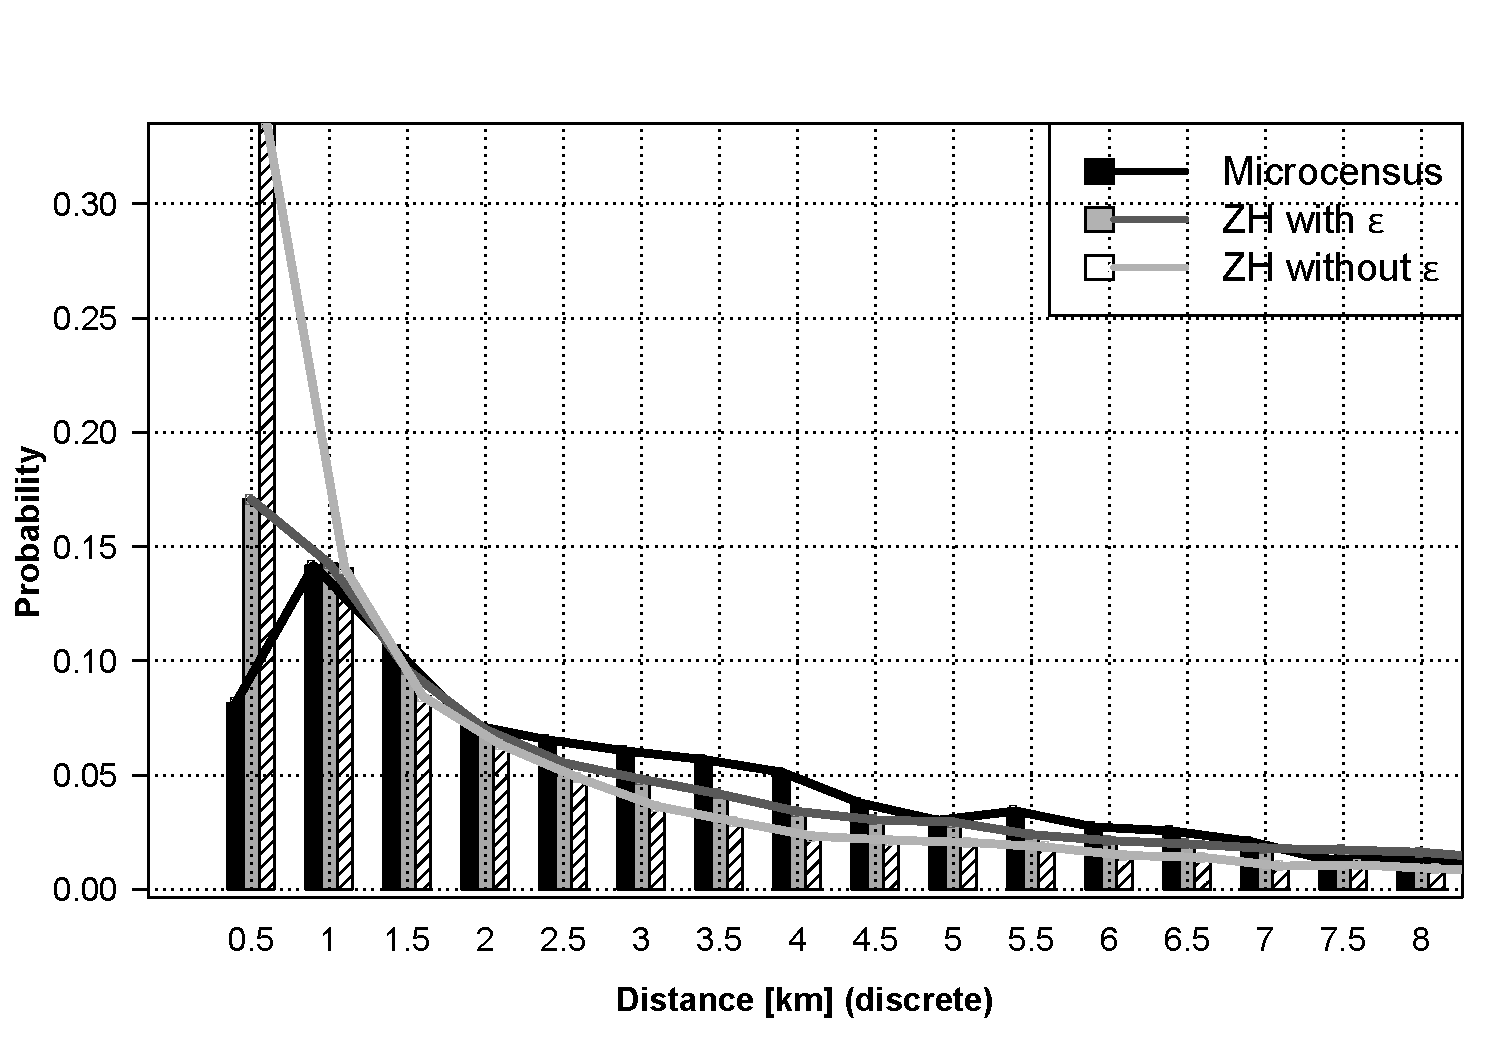
\includegraphics[width=0.99\textwidth,angle=0]{extending/figures/dc/zhShopping.pdf}}%
  {\label{fig:zhShopping}}%
  {}%
   \createsubfigure%
  {Leisure trips}%
  {\includegraphics[width=0.99\textwidth,angle=0]{extending/figures/dc//zhLeisure.pdf}}%
  {\label{fig:zhLeisure}}%
  {}%
}%
{}

\createfigure%
{Daily traffic volumes for 123 links compared to traffic counts}%
{Daily traffic volumes for 123 links compared to traffic counts. Per link $k$ the relative error is used, i.e, $(vol_{simulated,k}-vol_{counted,k}) / vol_{counted,k}$.}%
{\label{fig:countsLEGO}}%
{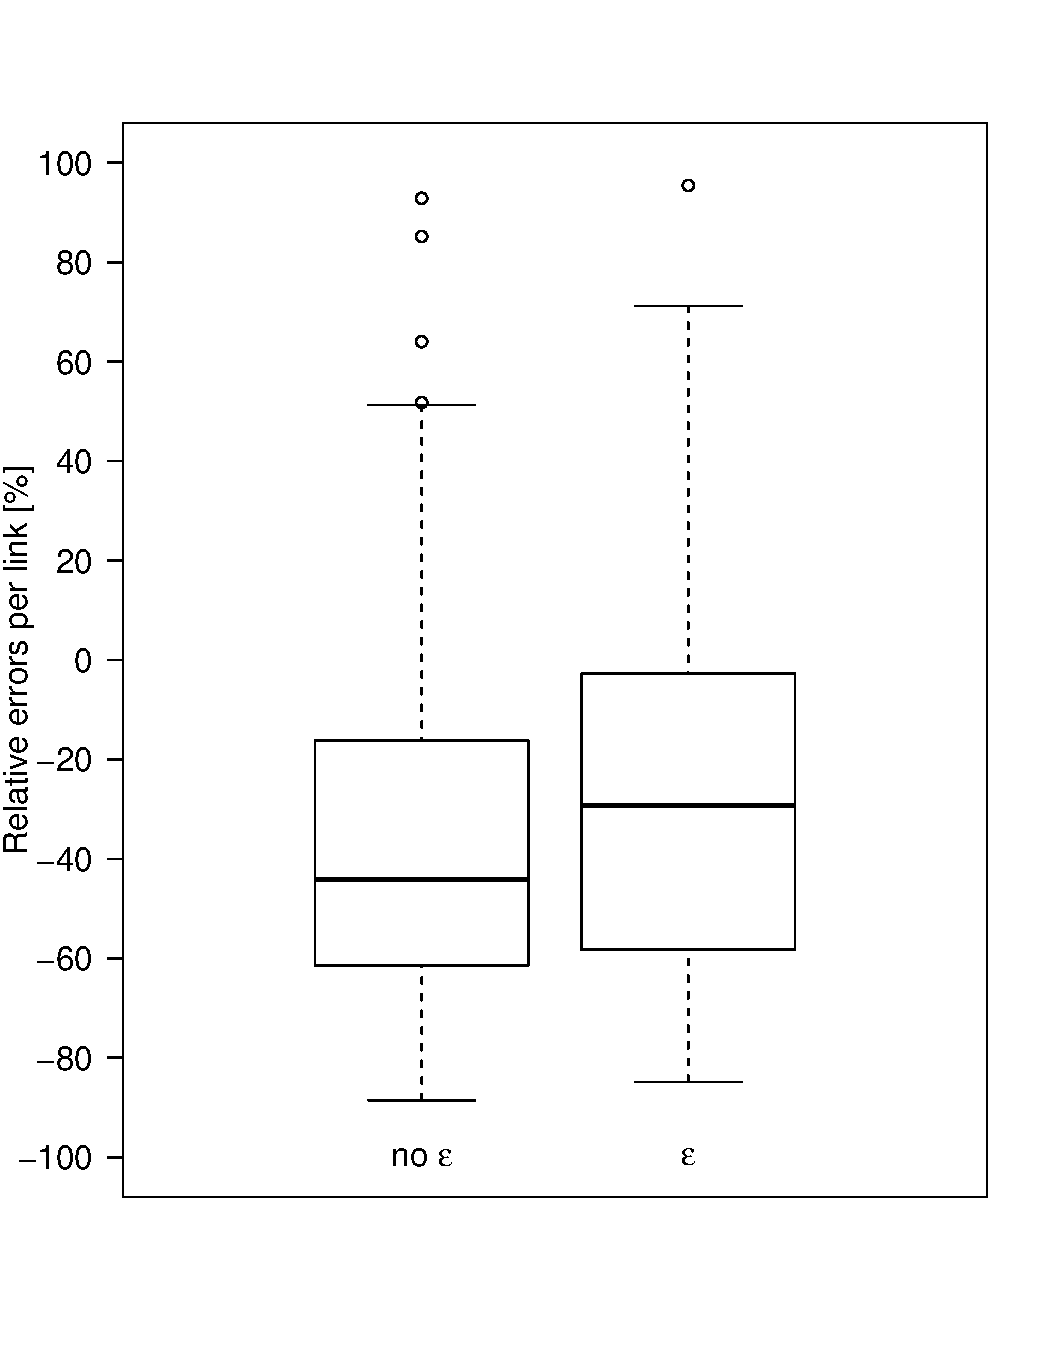
\includegraphics[width=0.8\textwidth, angle=0]{extending/figures/dc/zhCounts.pdf}}%
{}

% ##################################################################################################################
\section{Key Problems in Developing the Module}
Key problems of integrating destination choice into MATSim span behavioral and algorithmic issues. On the behavioral side, the specification of choice sets for model estimation is an unsolved problem to date. On the algorithmic side, as mentioned above, destination choice is in principle an ordinary optimization problem. However, as the agents interact and as the choices are embedded in a highly dynamic context, the problem becomes complex, even more as the targeted scenarios are usually large-scale. Thus, as is common for real-world optimization problems, solutions have to be based on problem-tailored heuristics \citep[][]{MichalewiczFogel_2004}. Important components of the MATSim destination choice are the construction of a limited search space and of the succeeding evaluation of this search space's elements. The main component however, is a mechanism to generate consistent random draws over the iterations necessary to include the objective function's error terms. This mechanisms is also applicable for other choice dimensions.

% --------------------------------------------------------------------
\subsection{Quenched Randomness}
In random utility theory, decision makers are assumed to be rational utility maximizers, where the utility is dependent on the characteristics of the alternatives, the choice maker itself and the choice situation. Besides these deterministic components, unobserved heterogeneity must be added by random error terms, often denoted $\varepsilon$. Due to these random error terms choices are quantified by probabilities dependent, for the logit model for example as $p_{n\ell q} = \exp(V_{n\ell q}) / \sum_L exp(V_{njq})$, where $V_{n\ell q}$ is person $n$'s systematic utility of alternative $\ell$ for activity $q$, which is divided by all remaining choice set's alternatives $j$. When drawing from the distribution specified by $p_{n\ell q}$ for a population, the aggregate choices are reproduced. This is basically also true, when applied in iterative frameworks. However, iterative frameworks are usually associated with some kind of learning or relaxation mechanism. This mechanism is heavily distorted by repeatedly and randomly drawing from $p_{n\ell q}$ in every iteration. In this case the $\varepsilon_{n\ell q}$ fluctuate from iteration to iteration, which is disastrous for the algorithm's convergence and behaviorally implausible.

Instead, the random error terms $\varepsilon$ need to remain fixed from iteration to iteration. The optimization is then performed as a deterministic search based on the resulting utilities $U_{n\ell q}$, i.e., an alternative $\ell$ for person $n$ and activity $q$ is selected as 
\[ 
\underset{\ell \in choice\: set}{\operatorname{argmax}} U_{nq} \,.
\] 
This includes, via the systematic part $V_{n\ell q}$, the disutility of traveling to destination~$\ell$ for activity~$q$.

As stated above, the random error terms need to remain the same over the iterations. In physics, this approach would be called ``quenched'' randomness; all randomness is computed initially and then attached to particles or destinations, rather than instantaneously generating it, which would be called ``annealed'' randomness. Two natural approaches for implementing quenched randomness are as follows:
\begin{itemize}
\item[(a)] Freezing the applied \emph{global} sequence of random numbers, meaning that a Monte Carlo method with the same random seed is used before and after the introduction of a policy measure and over the course of iterations. Thus, the error terms should come out the same way \emph{before} and \emph{after} the introduction of the policy measure. Differences in the outcome can thus be directly attributed to the policy measure. 
\item[(b)] Computing and storing a separate $\varepsilon_{n\ell q}$ for every combination of person $n$, alternative~$\ell$ and activity $q$.
\end{itemize}
 
Both strategies have flaws. Approach (a) is only an option if one is certain about every single aspect of the computational code. Importantly, one additional random number, drawn in one run but not in the other, completely destroys the ``quench'' for all decisions computed later in the program. Consistency is thus hard to achieve, especially in parallel or even distributed computing environments; according to personal communication a substantial machinery is necessary ensuring consistent choices. In a modular environment, as in MATSim, designed for external plugging-in of users' own modules---possibly drawing their own random numbers---the danger of destroying the quench is prohibitively high and thus approach (a) is impractical.

Approach (b) is certainly more robust. However, for large numbers of decision makers and/or alternatives, storing error terms is difficult. For destination choice, one quickly has $10^6$ decision makers and $10^6$ alternatives, resulting in $4 \times 10^{12} \hbox{Byte} = 4 \hbox{TByte}$ of storage space.

One may argue that this should not be a problem, since a normal person will rarely consider more than the order of a hundred alternatives in their choice set, reducing the computational problem. Aside from the necessity of storing every decision maker's choice set, this converts the computational problem into a conceptual one, since a good method to generate choice sets then needs to be found. With more conceptual progress, this may eventually be an option, but at this point, a conceptually simpler approach is preferred.

The developed solution below is generally applicable in econometric microsimulators. The same \emph{stable} error term can be \emph{re-}calculated on the fly by using stable random seeds $s_{n\ell q} = g(k_n, k_\ell, k_q)$, where are uniformly distributed random numbers associated with $k$, $\ell$, and $q$. That is, for each person $n$ a random number $k_n$ is generated and stored, and the same is done with each destination $\ell$. The value for the activity $q$ can be derived from its index in the plan possibly combined with the person's value $k_n$. This reduces the storage space dramatically from $\bar{nq} \times nn \times n\ell$ to $\bar{nq}(nn + n\ell)$, where $nn$ is the number of persons or agents and $n_\ell$ is the number of destinations and $\bar{nq}$ is the average number of discretionary activities in an agent's plan. This means that storage space is reduced to approx. $2 \times 4 \times 10^{6} \hbox{Byte} = 8 \hbox{MByte}$, which can be easily stored even on any modern machine.

The distribution of these seeds is essentially irrelevant; any error term distribution can be generated from any basic seed distribution. 
In the current version $g(k_n, k_\ell, k_q) = (k_n + k_\ell + k_q) \times v_{max}$ is used. $v_{max}$ is the maximum (long) number that can be handled by the specific machine.

To evaluate utility for a person $n$ visiting the destination $\ell$ for activity $q$ a sequence of Gumbel-distributed random numbers $seq_{n\ell q}$ is generated on the fly for every person-alternative-activity combination using the seed $s_{n\ell q}$. Some random number generators have problems in the initial phase of drawing, e.g., the first couple of random numbers are correlated or do never cover the complete probability space. As in our procedure the random number generator is constantly re-initialized, for these technical reasons, the error term $\varepsilon_{n\ell q}$ is derived not from the first element but from the $m^{th}$ element of the sequence $seq_{n\ell q}[m]$. Here, $m$ is set to 10. This procedure is valid as the set of all  $m^{th}$ elements of all different sequences is also a pseudo-random sequence following the same distribution as the sequences $seq_{n\ell q}$; clearly, \emph{true} random number generators relying on physical phenomena, such as hardware temperature, are not applicable. 

% ------------------------------------------
\subsection{Search Space Construction and Evaluation}
MATSim destination choice is based on best-response rather than random mutation, i.e., in every iteration the currently best alternative is chosen. This works as long as the inter-iteration changes are small, which is usually given by the relatively small share of agents who re-plan. The best-response approach is adopted due to the usually huge number of alternatives in combination with the search space characteristics. As the discrete search landscape is characterized by random noise because error terms are not (or only locally) spatially correlated (see Figure \ref{fig:landscape0}). For such problems---as opposed to continuous landscapes (see Figure \ref{fig:landscape1})---efficient search methods, such as local search methods, generally do not work.

% ---------------------------------
\createfigure%
{Search space}%
{Search space: The search algorithm is required to be able to handle correlated but also uncorrelated error terms as given by the MNL model. Local search methods, such as hill-climbing algorithms are only able to handle continuous search spaces, thus, for situation (a) a best-response global search algorithm is required.}%
{\label{fig:landscape}}%
{%
  \createsubfigure%
  {Uncorrelated error terms}%
  {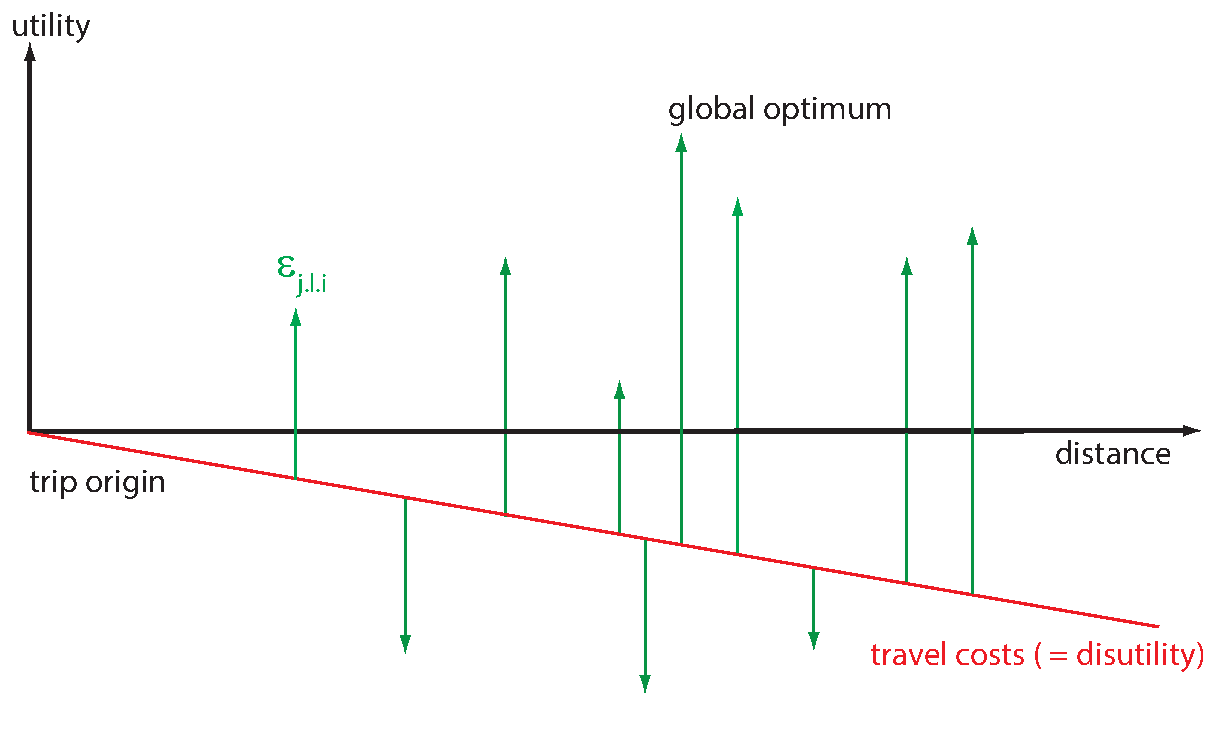
\includegraphics[width=0.8\textwidth,angle=0]{extending/figures/dc/landscape1.pdf}}%
  {\label{fig:landscape0}}%
  {}%
  \createsubfigure%
  {Spatially correlated error terms}%
	{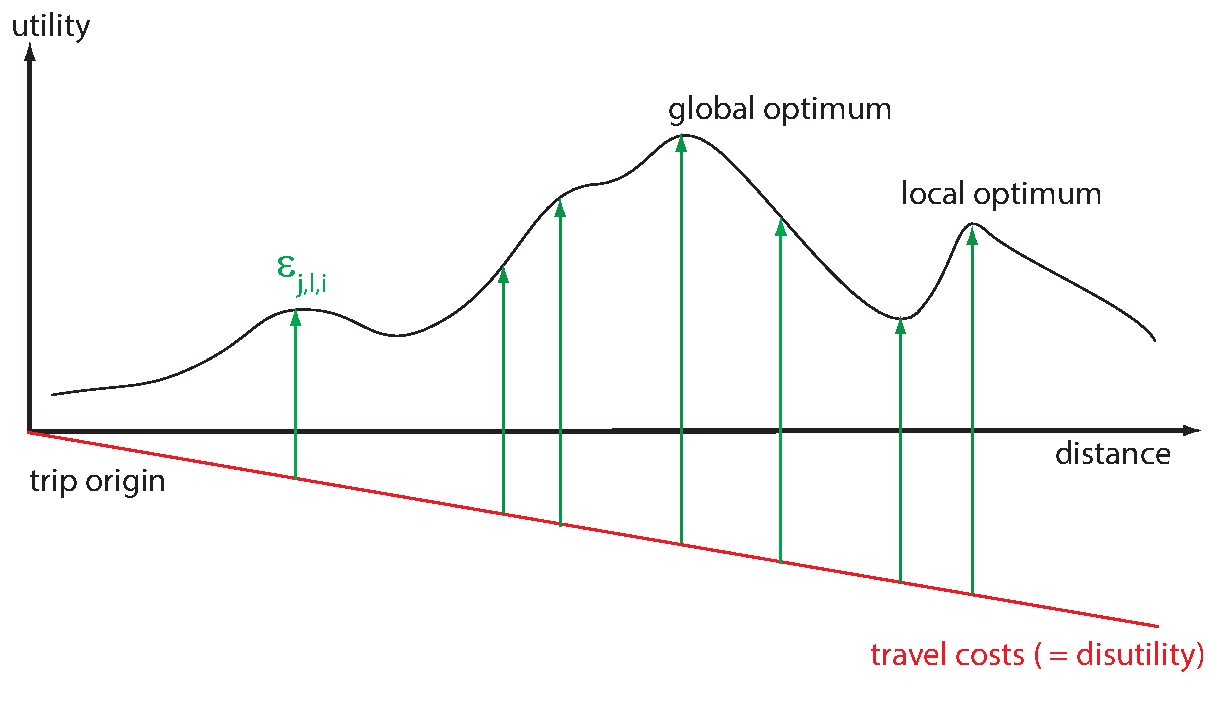
\includegraphics[width=0.8\textwidth,angle=0]{extending/figures/dc/landscape0.pdf}}%
  {\label{fig:landscape1}}%
  {}%
}%
{}

% ---------------------------------
On the search for the best choice, the large number of alternatives---prohibiting exhaustive search---is restrained as follows (for the detailed derivation see \citet[][p.51 ff.]{Horni_PhDThesis_2013}). It is assumed that travel costs are always negative, and that a person drops activities with negative net utility. Then the maximum potential travel effort a person is willing to invest is constrained by the maximum error term per person and activity. This approach is promising, as very large values for Gumbel-distributed are rare, meaning that a huge space must be searched for only a few persons. 

This reduction of the search space saves a lot of computation time, however, it is still infeasible and further speed-ups are necessary. Most computation time is due to calculation of travel times, i.e.,\ due to routing, for evaluation of the alternatives in the search space. To reduce these huge routing costs, the Dijkstra is not only applied forward---providing one-to-all travel times--but also \emph{backwards} using an average estimated arrival time as initial time. This is an approximation, and thus a \emph{probabilistic} best response is applied, justified by the natural assumption that, during the course of the iterations, the probabilistic choice probably reduces, or even compensates, the errors incurred by approximating travel times. 

With this procedure, the required computational effort is dramatically reduced, allowing application of destination choice to large-scale scenarios.

% ------------------------------------------
\subsection{Destination Choice Set Specification:}
While choice set specification is natural for choices with few alternatives, in contrast, for problems with a large universal choice set, usually present for spatial choices, such as destination or route choice, specifying individual choice sets becomes a challenging computational and even more behavioral issue (see e.g., \citet[][]{PagliaraTimmermans_TransLett_2009, Thill_PHG_1992, Schuessler_PhDThesis_2010, FrejingerEtAl_TransResB_2009}. Estimated parameters are sensitive to choice sets, and, at the same time, no established choice set definition procedure exists for spatial problems. This means that choice sets and, hence, estimation results are highly dependent on the modeler, which is an exogeneity problem, structurally similar to the well-known ``Modifiable Areal Unit Problem'' (MAUP), where results are dependent on modeler's zoning specification.

A prominent extension of the standard discrete choice modeling approach to treat this problem is formed by stochastic choice set models, founded by \citet[][]{Manski_TD_1977, BurnettKPHanson_TRR_1979, BurnettKP_UG_1980}, which integrates the choice set formation step into the estimation procedure by jointly estimating selection of a choice set and the choice of a particular alternative of this choice set \citep[][]{KaplanEtAl_TRB_2009, PagliaraTimmermans_TransLett_2009, Manski_TD_1977, Swait_TransResPartB_2001, HorowitzLouviere_IJRM_1995, BenAkivaBoccara_IJRM_1995, SwaitBenAkiva_TransResPartB_1987, Swait_TransResPartB_2001, MartinezEtAl_TransResPartB_2009, CascettaPapola_TransResPartA_2009, BierlaireEtAl_2_STRC_2009, ScroginEtAl_TechRep_UCF_2004, ManraiAndrews_EJOR_1998, Ansah_TransRes_1977}. Probabilistic choice set formation is conceptually appealing as choice sets are, in principle, not restrained a priori by exogenous criteria as in standard choice set specification. However, the procedure is in general associated with combinatorial complexity, making it computationally intractable. As a consequence, the practical approaches also require mechanisms to reduce the complexity of the choice set specification problem (see e.g., \citet[][p.11]{BenAkivaBoccara_IJRM_1995}). \citet[][]{ZhengJieGuo_TRB_2008}, for example, make the moderate assumption of continuous store choice sets (i.e., sets without ``holes'') around the trip origin, while the random-constraints model of \citet[][]{BenAkivaBoccara_IJRM_1995} exploits additional information on alternatives' availability for individuals.

Concluding, the destination choice set specification problem is still unsolved, meaning that the estimated models can only be fully consistently applied for the region, where the model was estimated. For MATSim, first destination choice model estimation efforts are reported in \citet[][Chapter 5]{Horni_PhDThesis_2013}.

% ##################################################################################################################
\section{The Module in the MATSim Context}
The destination choice module explicitly incorporates unobserved heterogeneity through random error terms. The standard MATSim utility function, however, does not contain error terms. The randomness measured in empirical data is included implicitly and in an uncontrolled way through the stochasticity of the simulation process. For destination choice, this has led to a dramatic underestimation of total travel demand making inclusion of unobserved heterogeneity inevitable. In the future, it should be researched if the standard utility function might also profit from the innovations of the destination choice module.

MATSim replanning offers different strategies to adapt plans ranging from random mutation to approximate suggestions, to best response answers. Destination choice is based on best response due to the sheer size of the alternatives set. 

As discussed in Chapter \ref{ch:scoring}, final goal is the implementation of an estimated utility function. At the moment, however, the standard MATSim scoring is still based on the Charypar-Nagel function and extended ad hoc by few attributes. This is also true for the destination choice module. Thus, calibration---instead of estimation---of the utility function is performed such that measured travel distances are matched. Calibration is performed by scaling the error terms. 

Although, the destination choice utility function is based on the discrete choice framework, some conceptual differences to the common application of discrete choice models exist. As shown above, there is no drawing from discrete choice models but maximization of an iteration stable utility function. In relation to that, the set of alternatives is not necessarily limited a priori and, thus, has the notion of a search space and not of a choice set.

% ##################################################################################################################
\section{Lessons Learned}
Two interesting lessons have been learning while developing the destination choice module. The first is a lesson of interdependence of preferences and space and,  thus, the necessity to evaluate them in combination. When looking at distance distributions (e.g., Figure \ref{fig:zhLEGO}) one might think that the functional form directly represents the preferences. This is not necessarily the case. In our simulations, it is the result of a \emph{linear} travel disutility applied in geographic space, where the number of opportunities increases with the square of the radius, in other words, with the travel distance. A similar emergent effect is present when scaling the random error terms. Although, both negative and positive error terms are enlarged and the average remains stable, the distribution gets more skewed toward the tail, as for the agents' choices the maximum values and not average values are relevant.

The second lesson concerns simulation results' variability. Although, random elements are not only present in destination choice, it was at the time of its development, the largest contributor of endogenous variability and made necessary the experiments presented in Section \ref{sec:variability}.

% ===============================================================================================
\section{Further Reading}
The main information source is \citet[][]{Horni_PhDThesis_2013}. Technical details and documentation are available at \citet[][]{MATSIM-T-DC_Webpage_2014}. Further reading related to destination choice is \citet[][]{HorniEtAl_IATBRspec_2013}, looking at parking, or \citet[][]{HorniEtAl_TechRep_IVT_2012}, coupling customers' and retailers' choices or in other words the supply and the demand side.

% ################################################################################################################## \cleardoublepage

\chapter{Within-Day Replanning}
\label{ch:withinday}
% ##################################################################################################################

\hfill \textbf{Authors:} Christoph Dobler, Michal Maciejewski, Kai Nagel

\begin{center} 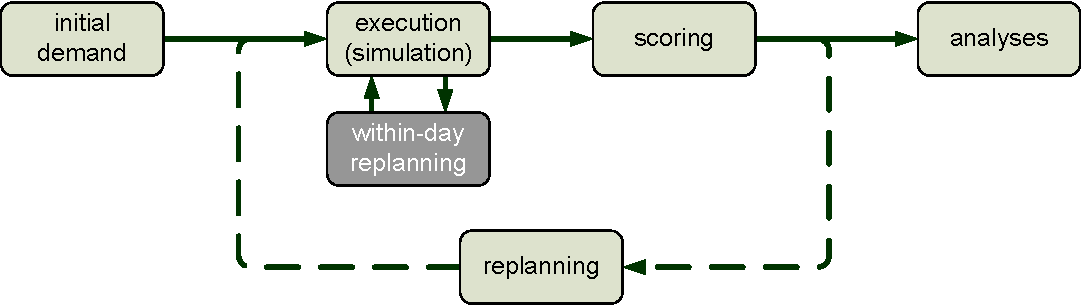
\includegraphics[width=0.6\textwidth, angle=0]{extending/figures/WithinDayReplanning/WithinDayMATSimLoop} \end{center}

\createStandardInformation{todo}{todo}{todo}{todo}

% ##################################################################################################################
\section{Introduction}
In recent years, in transport planning and traffic management the interest in scenarios where events occur which cannot or only partially be foreseen has increased. Typical examples for events which can only partially be foreseen are taxis and car sharing. An agent that has a taxi trip in its plan can for example not know in advance which taxi will be available when the agent needs one. When using car sharing, an agent might walk to the car sharing station and check whether a car is available or not. In case it is not, the agent could either decide to wait or adapt its plan and switch to another mode. Examples for events which cannot be foreseen at all are road accidents, terrorist attacks or disaster such as earthquakes.

Traditional simulation approaches (as used in MATSim) optimize traffic demand using an iterative process. There, it is assumed that a typical situation is simulated where agents can rely on their experience from comparable situations, like previous iterations. Applying an iterative approach to a scenario with unexpected events results in problems like illogical agent behavior, producing false results. In the next section, these problems, as well as an alternative simulation approach, are presented. On one hand, this approach---called within-day replanning---simulates only a single iteration, avoiding problems resulting from an iterative simulation process. On the other hand, this approach does require a more detailed behavioral model for the agents. Subsequently, using MATSim as a base, the iterative approach is discussed, followed by two different implementations of the within-day replanning approach into the framework including discussions of the technical implementations.

% ##################################################################################################################
\section{Simulation Approaches} 
\label{sec:SimulationApproaches}
% ============================================================================================
\subsection{Iterative Simulation Approaches} 
\label{sec:IterativeSimulationApproaches}
The starting point of an iterative simulation approach, as it is used in agent-based traffic flow micro-simulations like DYNEMO \citep{Schwerdtfeger_VolmulerHamerslag_1984, NoekelSchmidt_NSE_2002}, MATSim \citep{Balmer_PhDThesis_2007, BalmerEtAl_HEUREKA_2008} or TRANSIMS \citep{SmithEtAl_NTRPAC_1995, NagelRickert_ParComp_2001},  is the generation of an initial plan for each agent (e.g.,\,based on census and~/~or travel diary data). A plan contains an agent's intended schedule of activities and the trips that connect them. For each activity, its type (e.g.,\,\emph{work}, \emph{leisure} or \emph{shopping}), its location and the expected start and end time are given. A transport mode and a route specify a trip. The iterative optimization process consists of three steps. First, a mobility simulation executes the plans which are then evaluated using a fitness function. Finally, agents must select plans to be executed in the next iteration. Each agent can keep several plans in its memory. Bad plans can be deleted and new plans created by cloning and adapting existing ones using information (e.g.,\,travel times) from one or more previous iterations. The allowed adaption operations define the optimization search space (e.g.,\,routes, location and start / end times of activities). This iterative optimization can be seen as a period-to-period replanning strategy. Since one day is a commonly used duration, it is often called day-to-day replanning strategy.

An iterative day-to-day replanning approach is appropriate as long as the scenario describes a typical situation or day. For such scenarios, it is feasible to assume that agents are familiar with typically occurring events like traffic jams during peak hours. Therefore, they try to avoid driving during those times, or use alternative routes with less traffic. However, if the scenario contains unexpected events that the agents cannot foresee (e.g.,\,accidents or heavy weather conditions), using an iterative approach is not the best choice. First, user equilibrium will not be reached in such a scenario because agents do not have enough information to choose optimal routes and daily activity plans. Another problem is the optimization process itself. Even if an agent chooses its routes randomly due to a lack of information, it will eventually find a good route if it tries enough different routes.

%---------------------------------------------------------------------
\createfigure%
{Exceptional event in a network}%
{Exceptional event in a network}%
{\label{fig:labelExceptionalEventExample}}%
{%
  \createsubfigure%
  {Network with planned route}%
  {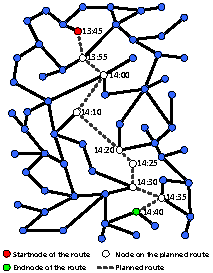
\includegraphics[width=0.43\textwidth, angle=0]{extending/figures/WithinDayReplanning/network_original_route}}%
  {\label{fig:labelNetworkPlannedRoute}}%
  {\qquad}%
  \createsubfigure%
  {Network with exceptional event}%
  {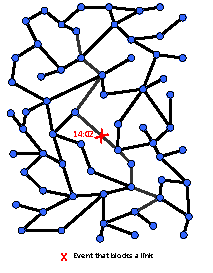
\includegraphics[width=0.43\textwidth, angle=0]{extending/figures/WithinDayReplanning/network_exceptional_event}}%
  {\label{fig:labelNetworkExceptionalEvent}}%
  {\vspace{5mm}}%

  \createsubfigure%
  {Network with exceptional event and planned route}%
  {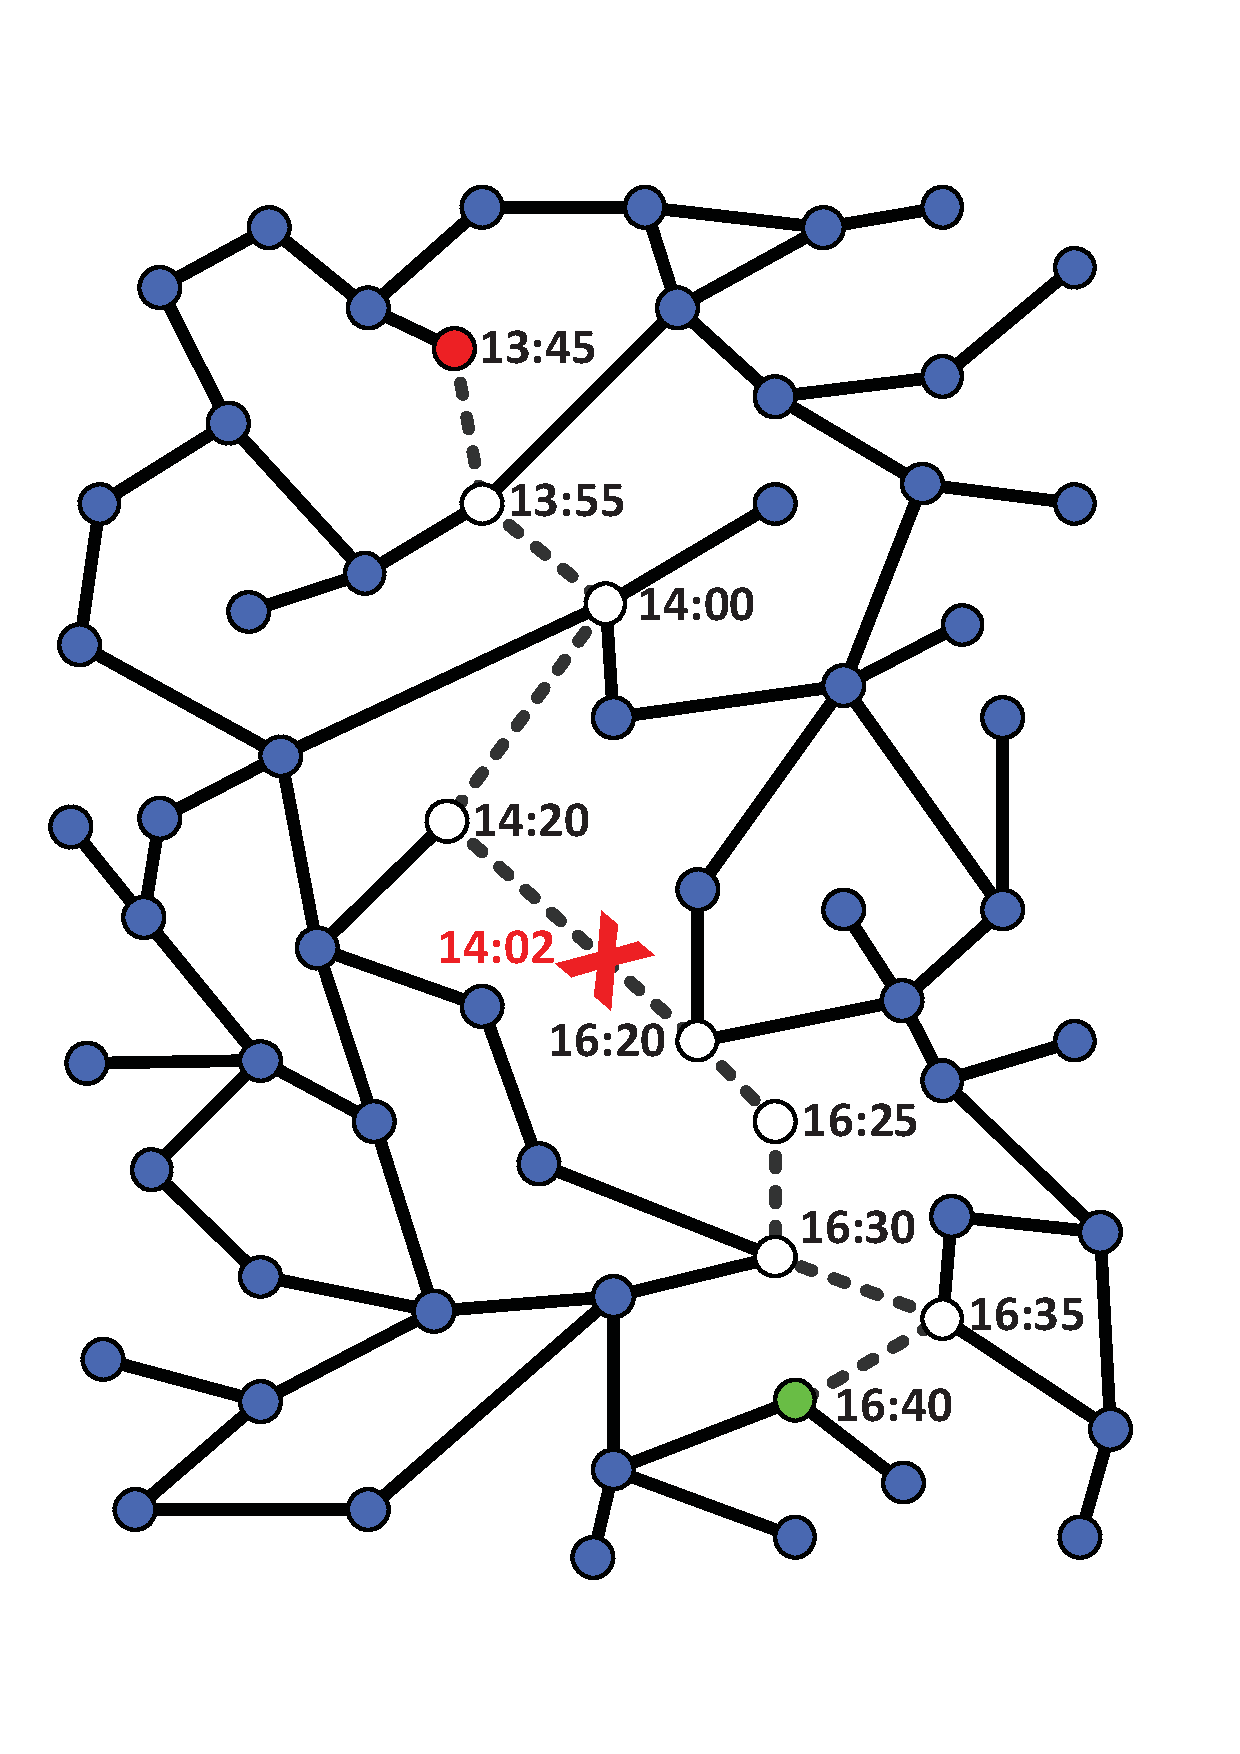
\includegraphics[width=0.43\textwidth, angle=0]{extending/figures/WithinDayReplanning/network_original_route_with_event}}%
  {\label{fig:labelNetworkExceptionalEventPlannedRoute}}%
  {\qquad}%
  \createsubfigure%
  {Network with exceptional event and adapted route}%
  {\includegraphics[width=0.43\textwidth, angle=0]{extending/figures/WithinDayReplanning/network_adapted_route_with_event}}%
  {\label{fig:labelNetworkExceptionalEventAdaptedRoute}}%
  {}%
}%
{}
%---------------------------------------------------------------------

Figure \ref{fig:labelExceptionalEventExample} shows a simple example scenario where an iterative approach would produce illogical and faulty results. In Figure~\ref{fig:labelNetworkPlannedRoute} an agent's planned route in a sample network is shown, including the times when the driver passes each node of the route. Clearly, those times are only valid if no exceptional event occurs. Figure~\ref{fig:labelNetworkExceptionalEvent} shows a link where an event, like an accident, blocks that link for two hours. As a result, the agent reaches its destination two hours later than expected (Figure~\ref{fig:labelNetworkExceptionalEventPlannedRoute}). When this scenario is iterated, the agent recognizes that its route has a much higher travel time than expected and therefore it will choose another route. The traffic jam caused by the accident will probably also increase travel times on links next to the blocked link. Therefore, the agent might find a route which is quite different than the original one (Figure~\ref{fig:labelNetworkExceptionalEventAdaptedRoute}). A closer look at the node where the new route deviates for the first time from the original one shows that this occurs even before the accident happened, which is unfeasible and illogical.

An obvious solution to avoiding such problems is using an alternative simulation approach without an iterative optimization process. The next section discusses such an approach and the requirements that must be fulfilled.

% ============================================================================================
\subsection{Within-Day Replanning Approach}
A within-day replanning approach uses a significantly different strategy from that of an iterative approach. Instead of multiple iterations, only a single one is simulated. Thus, it is now essential that agents can adapt their plans during this iteration without having information from previous iterations available. To do so, they have to continuously collect information and take into account their desires, beliefs and intentions when they decide how to (re)act.

While iterative approaches can use best-response modules, a within-day approach has to use something that might be called a best-guess module. Travel times are an obvious example. In an iterative approach, travel times can be collected from the previous iteration or even be averaged over several past iterations. The nearer a stable system is to a relaxed state, the smaller the differences in travel times between two iterations. This is not possible in a within-day approach. Even if an agent has perfect knowledge, it can only assume how the traffic flows will evolve in the future. To do so, it can take different information into account to estimate travel times. It could, for example, take travel times from a typical day without exceptional events and combine them with information it gathers during the simulated day. Depending on the amount and the quality of this information, the agent might rely more or less on its experience.

Therefore, the decision-making process of an agent becomes an important topic. In an iterative approach, each agent has total information and can thus select the best route. Due to limited available information, this is not possible in a within-day approach. One agent could, for example, choose a route where expected travel time is very short, but also very uncertain. Another agent might not be willing to take that risk and therefore select a longer route where the assumed travel time is more reliable. Perception of information might also vary between agents; one could rely on media traffic information, another might ignore it.

Each within-day replanning action is categorized by two parameters---the replanned element of the plan (an activity or a trip) and the point in time when the replanned plan element is executed (right now or at a future point in time). If an activity is replanned, several changes are possible. Its start and end time can be adapted, its location can be changed, it can be dropped, or created new from scratch. For a trip, origin and destination, route, mode of transport and departure time can be replanned. Often replanning one single plan element results in a chain reaction that forces replanning of other plan elements. If, for example, an activity is dropped, the trips from and to this activity have to be merged.

The second parameter categorizing a replanning action depends on when the replanned plan element is executed. This could be either the currently performed plan element or one being performed in the future. Clearly, in a currently performed plan element, not all previously mentioned replanning actions could be conducted. E.g.,\,start time of an activity or transport mode of a trip currently being performed can no longer be adapted.

Due to the limited available information, a within-day replanning approach will, in contrast to an iterative approach, not converge to a user equilibrium. Decisions made during the simulated time period may seem to be optimal when they are made. However, evaluated retrospectively, an agent might realize that they were not.

Figure \ref{fig:labelWithinDayMATSimLoop} shows how within-day replanning can be integrated into MATSim's iterative optimization loop. An additional block builds another (inner) loop with the mobility simulation. Depending on the type of simulated scenario, the outer loop can be skipped.
%---------------------------------------------------------------------
\createfigure%
{(Iterative) within-day replanning MATSim loop}%
{(Iterative) within-day replanning MATSim loop \kai{I think this figure needs to come earlier, i.e.,\,in Section~\ref{sec:SimulationApproaches} \textbf{TODO: redraw this figure using the new (blue) matsim loop?}.}}%
{\label{fig:labelWithinDayMATSimLoop}}%
{\includegraphics[width=12.5cm, angle=0]{extending/figures/WithinDayReplanning/WithinDayMATSimLoop}}%
{}%
%---------------------------------------------------------------------

% ============================================================================================
\subsection{Combined Approaches} 
\label{sec:CombinedApproaches}
An alternative to iterative or within-day replanning only approaches, is to combine them. An obvious application is solving situations that cannot be planned exactly in advance, like parking or car sharing. An agent is, for example, able to plan a parking activity, but it cannot anticipate which parking spots will be available when the agent arrives. Thus, within-day replanning can be used when the agent starts its parking choice.

Other agents might want to share their cars, so an actual meeting must be confirmed. This can be ensured using within-day replanning. If the driver arrives too early, a \emph{waiting} activity is added to its plan; otherwise the agent being picked up will perform a \emph{waiting} activity until the car arrives.

% ##################################################################################################################
\section{Implementation}
% ============================================================================================
\subsection{General Thoughts}
Within-day or en-route replanning means that travelers replan during the day or while they are on their route.  This means that the simulation needs to find some way to influence the agent while the mobility simulation (network loading) is running. For the MATSim main network loading module, the so-called \lstinline$QSim$, this could be achieved by inserting an agent-loop, as follows:
\begin{lstlisting}
   void doSimStep() {
      for ( each agent ) {   // <-- agent loop
         agent.doSimStep() ;
      }
      for ( each link ) {
         link.doSimStep() ;
      }
      for ( each node ) {
         node.doSimStep() ;
      }
   }  
\end{lstlisting}
In this loop, each agent has the chance to deliberate in every time step.  Clearly, the agent can decide that he/she has nothing to deliberate and return immediately.

Such an approach does, however, lead to computational challenges. Going through all links and nodes in every time step is already an expensive operation, and a number of efficiency improvements (such as "switching off non-active links") are contained in the code.  Also, the number of links or nodes is typically an order of magnitude smaller than the number of synthetic persons in a scenario. Thus, some massive optimization would have to be undertaken in order to make the above approach computationally efficient.

An alternative approach to the above is to ask each agent only when a decision needs to be taken. The most important decision for a driver is to chose the next link, i.e.,\,\begin{lstlisting}
class MyDriverAgent implements DriverAgent {
   ...
   @Override
   public Id<Link> chooseNextLink() {
      <algorithm to determine ID of next link>
      return nextLinkId ;
   }
}
\end{lstlisting}
%
Similar implementations are needed for all other queries that could be asked of the agent, for example
\begin{compactitem}
\item Should the trip end on the current link?
\item Should the agent alight at the current stop?
\item What is the ID of the vehicle to be used for a trip?
\end{compactitem}
%
From the perspective of the agent such an approach might be called \emph{event driven}, since the agent performs mental activity only at such events.

There is, indeed, a mechanism to program such agents and to insert
them into the \lstinline$QSim$. This is discussed in more detail in Section~\ref{sec:impl-repl-the-ag}.

A challenge with that approach is that the complete agent needs to be re-programmed.  This agent needs to have enough capabilities to be oriented about itself; for example, it needs to be able to compute plausible routes.

On the other hand, there are situations where the capability to decide the turn at each intersection while en-route is, in fact, not needed.  
%
For example, for typical evacuation applications it makes sense to start all agents on their normal daily plans. When an emergency warning is distributed, the simulation can go once through all agents and decide how they react.  This will be done by replacing some or all future elements of the current plan.  In some applications this may happen more than once, for example if the recommended evacuation directions change because of a change in wind direction.  In other applications, evacuating agents may become stuck in unexpected congestion which may trigger en-route re-routing. This may, however, be restricted to relatively small regions, and it may be sufficient to go through such a replanning loop every, say, 300\,simulated seconds. 

For such applications, the plan-based approach (Section~\ref{sec:impl-plan-based}) is more suitable.  Rather than having each agent answering certain queries in every time step or at every intersection, the plan-based approach first waits for a trigger (such as an emergency warning, or unexpected congestion), then decides on the affected agents, and then goes through those agents and changes the future portion of their plans. This is not only conceptually easier than having every agent to answer for him-/herself, but it is also computationally more efficient since it is only called when it is triggered, and for the affected agents. 

Overall, implementers and users will have to balance their needs.  
%
If there are relatively few times when agents should re-plan, and these times can be easily identified by, say, corresponding to an emergency signal, then this is an indicator for the plan-based approach.  
%
If, on the other hand, an agent goes into the simulation mostly or entirely without a plan, for example for an entirely reactive taxi driver, then this points to the approach of replacing the agent.

MATSim provides infrastructure for both approaches. The plan-based approach currently provides more support infrastructure, i.e.,\,many important use cases can be implemented by re-using existing methods.  The approach that replaces the agent, in contrast, provides more flexibility.  In particular, it makes it possible without additional computational overhead that agents make decisions at the latest possible time.  While this is not entirely realistic behaviorally, such an approach is often desirable from a simulation perspective, where one does not want reproducibility of simulations depend on, say, random elements in terms of how far an agent plans ahead.

% ============================================================================================
\subsection{Implementation Alternative 1: Plan-Based Implementation}
\label{sec:impl-plan-based}
\kai{Christoph, die ``mnote'' sind für mich, damit ich einen schnellen Überblick habe, was Du geschrieben hast.  Damit ich das nicht wiederhole, sondern mich ggf.\ darauf beziehe.}

\mnote{day-to-day loop no longer necessary}

When adding within-day replanning to MATSim, its iterative loop (see Figure~\ref{fig:matsimcycle}) has to be adapted as shown in Figure~\ref{fig:labelWithinDayMATSimLoop}. On one hand, the additional \emph{within-day replanning} module is added, which interacts with the mobility simulation. On the other hand, multiple iterations are only necessary if a combined simulation approach is used.

\mnote{implementation as MobsimEngine ... tracking agents and plans}

The implementation is realized as so-called \lstinline{MobsimEngine} which can be plugged into the \emph{QSim}. In every simulated time step, the \emph{QSim} iterates over all registered \lstinline{MobsimEngines} and allows them to simulate the current time step. Besides simulation of the traffic flows, those engines are also able to let agents start or end activities. The engine containing the within-day replanning logic (called \lstinline{WithinDayEngine}) does not simulate traffic flows but tracks agents and adapts their plans. Doing so is separated into two steps. First, agents whose plans have to be adapted in the current time step are identified. In a second step, the adaption of their plans is performed. 

\mnote{register identifiers with replanners, replanners with the within-day engine}

Figure~\ref{fig:labelWithinDayEngine} shows the structure of the \lstinline{WithinDayEngine}. Multiple \lstinline{Replanners} can be registered to the engine. Each \lstinline{Replanner} represents a unique replanning strategy like re-routing or time mutation and uses a set of \lstinline{Identifiers} which communicate with agents and select those agents who are given the opportunity to adapt their plans. An \lstinline{Identifier} can be seen as an information-distributing unit, like a radio station or a policeman. Therefore, not every \emph{Identifier} communicates with all agents. For example, agents at home will probably listen to the radio, but agents walking in the park will not. Each \lstinline{Identifier} returns a list of agents to its superior \lstinline{Replanner}, which then adapts those agents' plans.

%---------------------------------------------------------------------
\createfigure%
{WithinDayEngine}%
{WithinDayEngine}%
{\label{fig:labelWithinDayEngine}}%
{\includegraphics[width=8.0cm, angle=0]{extending/figures/WithinDayReplanning/ReplanningManager}}%
{}
%---------------------------------------------------------------------

\mnote{more about itentifiers and replanners}

There is a division of responsibilities between \lstinline{Replanners} and \lstinline{Identifiers}. The first ones are responsible for adapting the agents' plans but they should not check whether an agent should be replanned or not. If, for example, a \lstinline{Replanner} updates an agent's route, it has to be ensured by the \lstinline{Identifiers} that only agents who are currently performing a leg are replanned. In turn, \lstinline{Identifiers} should select agents who have to be replanned but should not change their plans. As a result of this division, the often time consuming replanning of the agents' plans can be performed using parallel threads which leads to an almost linear speed-up. In general, simulation results do not depend on the order in which agents are replanned. \emph{Replanners} which use random numbers are a special case. 
%They have to ensure that 
In the present implementation, their \emph{random number generator} is re-initialized for every replanned agent using a deterministic value (e.g.,\,a combination of the agent's Id and the current time step). On one hand, this ensures that an agent's decisions can be reproduced even when the global sequence of random numbers changes. On the other hand, the simulation outcomes do not change if the number of threads used for the replanning is changed.
% \kai{Christoph, ist es das?  ``have to'' (wie Du es vorher hattest), erscheint mir auf jeden Fall zu stark.  Oder hat es etwas mit multi-threading zu tun?}

\mnote{identifiers run sequentially}

Running the \lstinline{Identifier(s)} to select those agents who have to adapt their plans is performed sequentially. On one hand, an \lstinline{Identifier}'s runtime is typically very short and therefore no significant performance losses are expected. On the other hand, 
%it is a robust design which 
this makes the design robust so it cannot produce race conditions which could occur if multiple instances of an \lstinline{Identifier} run concurrently. An example would be an \lstinline{Identifier} which selects agents on household level, i.e.,\,if a member of a household is identified, also all other members are added to the list of agents who have to be replanned. In an approach with parallel running instances of an \lstinline{Identifier}, an instance could identify member A of a household while concurrently another instance could identify member B of the same household. As a result, the household's members would be twice in the list of agents to be replanned---once added by each \lstinline{Identifier} instance.

\mnote{different basic replanners for current/future trips/acts}

\lstinline{Replanner} implementations are available for every possible basic change of an agent's scheduled daily plan. Any trips and activities can be adapted, although some replanning operations are not available when trip or activity has already been started. Possible adaptations are:
\begin{compactitem}
    \item current trip (route, destination)
    \item future trip (add, remove, mode, route, origin, destination)
    \item current activity (end time)
    \item future activity (add, remove, location, type, start and end time)
\end{compactitem}
%
For complex plan adaptations, those basic \lstinline{Replanners} can be combined. If, for example, an agent currently performing a trip changes the destination of its next activity, routes of the current and next trip have to be adapted.

\mnote{different basic identifiers}

Additionally, four basic \lstinline{Identifiers} have been implemented so far. They identify agents, which are...
\begin{compactitem}
    \item performing an activity.
    \item performing an activity which will end in the current time step.
    \item performing a trip.
    \item performing a trip and are going to move to another link.
\end{compactitem}

\mnote{AgentFilters (e.g.,\,for spatial areas)}

Often, identifiers have to handle only a subset of the population, e.g.~only male agents or agents which are currently performing a car trip. In order to prevent that the same functionality has to be implemented multiple times, so-called \lstinline{AgentFilters} are introduced. Their task is to remove agents which do not meet the filter criteria from a set of agents. Using \lstinline{AgentFilters} not only avoids duplicated code but can also reduce the computation effort. An example would be two \lstinline{Identifiers} which should identify only agents currently traveling in a certain part of the network. Without \textit{AgentFilters}, each of them would have to track all traveling agents and their current positions. When this functionality is moved to an \lstinline{AgentFilter}, the two \lstinline{Identifiers} can share a single instance of that filter.

\mnote{filters: simple and re-usable; identifiers: complex and include decision-making}

Basically, simple and re-usable functionality should be implemented as \lstinline{AgentFilters} while more complex and/or decision making functionality should be part of an \textit{Identifier}. Again, this can be depicted with an example, e.g.,\,a scenario in which the search for a parking space is modeled. A filter can be utilized to take only agents into account which are currently traveling by car. The \lstinline{Identifier} solves the more complex tasks such as deciding when the agent starts its search or selecting the searching strategy to be applied.

\mnote{basic AgentFilters}

Three basic \lstinline{AgentFilters} have been implemented so far. They filter agents which are not...
\begin{compactitem}
    \item part of a predefined set of agents.
    \item currently using a transport mode included in a given set.
    \item currently located on a link included in a predefined set.
\end{compactitem}

\mnote{observers}

Besides the logic that identifies agents and adapts their plans, another important part of the within-day replanning framework is code that continuously collects information and provides it to the \lstinline{Identifiers} which decide based on that data whether agents are replanned or not. In a time step based approach---as it is realized by the \emph{QSim}---collecting, analyzing and aggregating data as well as providing it can be easily realized. Figure~\ref{fig:labelQSimTimeStep} shows the structure of a \emph{QSim's} time step. Each time step is separated into three phases---\lstinline{before time step}, \lstinline{do sim step} and \lstinline{after time step}. During the \lstinline{do sim step} phase, all registered \lstinline{MobsimEngines} simulate the current time step. The \lstinline{before time step} and \lstinline{after time step} phases allow to execute code before respectively after the simulation of the current time step. A class can collect data like link travel times during the \lstinline{do sim step} phase. Afterward, the collected data can be analyzed and aggregated in the \lstinline{after time step} phase. In the next time step, the \lstinline{WithinDayEngine's Identifiers} can use that data for their decisions. The \lstinline{WithinDayEngine} is always the first \lstinline{MobsimEngine} which executes its \lstinline{doSimStep} method. This ensures that no agent has changed its state since the \lstinline{after time step} phase of the previous time step. As a result, the \lstinline{Identifiers} make their decisions on %actual 
current data.

%---------------------------------------------------------------------
\createfigure%
{QSim time step}%
{QSim time step}%
{\label{fig:labelQSimTimeStep}}%
{\includegraphics[width=8.0cm, angle=0]{extending/figures/WithinDayReplanning/QSimTimeStep}}%
{}
%---------------------------------------------------------------------

\mnote{example: TravelTimeCollector}

An example for such a class is the so-called \lstinline{TravelTimeCollector}. Its task is to provide actual link travel times to the \lstinline{Replanners} by collecting and averaging travel times of agents that have recently passed a link during a given time span. A typical time span is 15\,minutes; older link travel times are ignored. Duration of the specific time span has an important impact on travel times reported to the \lstinline{Replanners}. On one hand, significant changes in link travel times will be communicated very slowly, if the time span is too long. On the other hand, a too short duration will overrate outliers.

The \lstinline{TravelTimeCollector} is a simple, but efficient implementation of a within-day travel time calculator. It does not implement features like traffic flow predictions or dynamic weighting of recent travel times based on historical data. 
%Due to 
Because of the abandonment of such features, it is very robust, even in scenarios where traffic flow conditions change dramatically.

%---------------------------------------------------------------------
\createfigure%
{TravelTimeCollector}%
{TravelTimeCollector}%
{\label{fig:labelTravelTimeCollector}}%
{\includegraphics[width=8.0cm, angle=0]{extending/figures/WithinDayReplanning/TravelTimeCollector}}%
{}
%---------------------------------------------------------------------

\mnote{matsim person vs.\ matsim agent}

The current MATSim code differentiates between \lstinline$Person$ and \lstinline$MobsimAgent$.  
%
\lstinline$Person$ can be seen as a very simple Q-learning entity, possessing multiple \lstinline$Plan$s ("actions"), each together with an expected score which is updated every time the plan is tried out. In consequence, a \lstinline$Person$ is persistent over the iterations; in fact, the internal state of each \lstinline$Person$ is written to file at the end of the iterations.
%
\lstinline$MobsimAgent$, in contrast, is instantiated every time the \lstinline$QSim$ is called, and does not exist beyond the running time of the \lstinline$QSim$. A \lstinline$MobsimAgent$ is essentially reactive, being queried by the framework about decisions when approaching intersections, arrival points, or public transit stops. In the standard implementation, these queries are answered by the plan, but other implementations can be used, and/or additional \lstinline$MobsimAgent$s can be added which do not correspond to \lstinline$Person$s.

\mnote{Which plan to modify}

This leads to the question if within-day adaptations to the \lstinline$Plan$ should be passed through to the \lstinline$Person$. Let us call the actual trajectory through the system the "executed plan"'.  This can be different from the original plan, for example using a different route, different departure times, different modes, etc. The original plan cannot just be replaced by the executed plan, since it is not clear that the executed plan, when used as input, will have itself as expected output. In consequence, it is not possible to treat the executed plan together with the just obtained score as an action-value pair in the sense of Q-learning, since the score was obtained from the \emph{original} plan, not from the executed plan.

In consequence, the code uses a copy of the original plan and modifies the copy. The score, however, is given to the original plan. The implementation is able to 
\kai{"is able to"? (existiert das derzeit als Option?}
%
\dobi{Christoph: sollte da sein, sofern der Code nicht inzwischen zerschossen wurde. Ich hatte das für den Initial Routes Creation Abschnitt in meiner Diss verwendet. Ich wollte da auch nochmal genauer drauf schauen, was die produzierten Ergebnisse eigentlich bedeuten - habe ich dann aber irgendwie nie mehr Zeit dafür gefunden.}
% 
\emph{also} memorize the executed plan and add it to the set of plans. This functionality, however, is experimental.

%% \mnote{lskdjf}

%% An important aspect that has to be considered when within-day replanning is used is whether the persons' or only the agents' plans are replanned. In this context, a person is a global object which exists during an entire simulation run. An agent represents a person in the (traffic flow) micro-simulation part of an iteration. Moreover, a person has several plans in its memory, an agent only a single one. By default, an agent's plan is only a copy of the plan of the person which is represented. Only the score of the person's plan is updated by MATSim's scoring module. 

\mnote{parking example: parking search route should not be added to plan}

One example where setting the original to the executed plan clearly does not make sense is parking search \kai{citation?}
\dobi{Christoph: keine. Eventuell könntem an den Absatz auch weglassen? Der Standard ist ja mittlerweile, dass man den Plan der Person nicht verändert. Andererseits wäre dann der Absatz unten (mit den initial Routes) eher interessant, weil der eben ein Beispiel dafür gibt, wo die Standardeinstellung nicht sinnvoll ist.}.
\ah{\citet[][]{WaraichEtAl_TechRep_IVT_2013_2, WaraichEtAl_TechRep_IVT_2012}. Komme weder an den einen noch an den anderen dran und kann die Frage deshalb nicht selber beantworten.}
%In a first one, within-day replanning is used to simulate agents' parking search. 
A person's plan contains as destination the location where a free parking space is expected. However, if the agent realizes in the mobility simulation that there is no free space left, it starts looking for a free parking spot. As a result, the agent's route is extended. This extension has to be local in the agent's route since it is only necessary in the current iteration
but maybe not in another one where the initially selected parking spot is available.

%% \mnote{starting agents without routes: within-day routes \emph{should} be added to plan (but I don't agree)}

%Creating agents' initial routes using within-day replanning would be an example for an application where persons' plans have to be adapted. By default, creation of those routes is a step performed on person level before the micro-simulation is started for the first time. When this task is moved into the micro-simulation and is performed during their runtime, the created routes have to be still stored in the person's plan. Otherwise they would not be available for later iterations. 
%\kai{Christoph, habe hier mal tentativ einen Absatz auskommentiert, der mir nicht wirklich hilfreich erscheint.  Solange der Plan, mit dem der Agent losfährt, derjenige ist, der den Score bekommt, ist es unerheblich, wann er berechnet wurde.}
%\kai{some pointers to simulations done with this set-up}

The capabilities of this within-day replanning implementation are shown and discussed by \citet{Dobler_PhDThesis_2013} based on two sets of conducted experiments. The first set is based on a model of Zürich city. There it is assumed that the capacities of several arterial roads in the city center are drastically reduced during the morning peak. Traveling agents are given the opportunity to bypass the resulting traffic jams by adapting their routes using within-day replanning. As a result, the average travel time of an agent affected by the incident is reduced from 42 to 23\,minutes. Another interesting finding is that even if only 50\,\% of the population adapts its routes still the average travel times are reduced to 25\,minutes.
%\kai{Christoph: Vielleicht noch einen Satz über Ergebnisse (oder den vorhergehenden Satz umschreiben: Agents bypass the resulting traffic jams by adapting ..., leading to an overall readuction of travel times XX sec compared to the solution where agents stick to their routes.} 

The second set of experiments uses within-day replanning to create agents' initial routes. The results are compared to runs where those routes are created before the simulation is started and without having traffic flow information available. It is shown that agents' average travel times are already very close to the values in a relaxed state. When using MATSim's traditional approach, 10 to 15\,iterations have to be performed before the average travel times have reached this level. %\kai{Christoph: Vielleicht noch einen Satz über Ergebnisse?}

\subsection{Implementation Alternative~2: Replacing the Agent}
\label{sec:impl-repl-the-ag}

According to \cite{RussellNorvigBook}, an agent is "anything that can be viewed as perceiving its environment through sensors and acting upon that environment through effectors."  As stated above, MATSim has agents on two levels:
\begin{compactitem}

\item \lstinline$Person$ is a Q-learning agent that is persistent over the iterations.

\item \lstinline$MobsimAgent$ is a reactive agent that only exists during the \lstinline$QSim$.

\end{compactitem}

For the Q-learning agent, perception works through the events, i.e.,\,events are used to compute the score, build mental models to generate alternatives, etc. Acting upon the environment works through the selection of the plan.

For the reactive agent, perception works more directly through callback methods, such as the simulation notifying the agent of just having moved over an intersection. Acting upon the environment works through making decisions at decision points, e.g.,\,about turning directions at intersections, or if to board a certain bus.

As said earlier, the approach described in Section~\ref{sec:impl-plan-based} assumes that the reactive agent still has, and most of the time follows, a plan. There may, however, be situations where this is not appropriate, for example when the agent makes up the route as it goes, or when quite in general one wants to investigate models where each agent has its own perception and deliberation, rather than some external algorithm modifying its plan. As also said earlier, there is no clear recipe when which approach is better; it depends both on the needs of the project and on the personal preferences of the developer.
%
Here, we will thus look at \lstinline$MobsimAgent$s which do no longer have a pre-compted plan but make decisions as they go. There is also a class \lstinline$DynAgent$, which wraps around the somewhat archaic \lstinline$MobsimAgent$, making it easier to use and providing additional infrastructure (Section~\ref{sec:dynAgent}).

% ----------------------------------------------------------------------------
\subsubsection{Agent Interface}
The \lstinline$DriverAgent$ interface structurally is something like
\begin{compactitem}
\item \lstinline$Id chooseNextLinkId()$ -- agent is asked at intersections and needs to return how to proceed.

%% \item \lstinline$Id<Link> getDestinationLinkId()$ -- agent is essentially asked if it wants to arrive on the current link.\footnote{%

%% The method can return {\tt null}.  Arguably, it should be modified to something like {\tt boolean isArrivingOnCurrentLink()}.

%% }  
\item \lstinline$boolean isWantingToArriveOnCurrentLink()$ -- agent is asked if it wants to arrive on the current link.
\item \lstinline$void notifyMoveOverNode(Id newLinkId)$ -- agent is notified that it has traversed the intersection and entered a new link.
\end{compactitem}
%
Everything else are relatively simple bookkeeping methods such as \lstinline$getId()$ -- the agent needs to know its own identifier.

If it is assumed that the agent does not only replan en-route but also while at activities, then also the \lstinline$MobsimAgent$ interface needs to be implemented.  This is a bit more involved; important methods are
\begin{compactitem}
\item \lstinline$endLegAndComputeNextState(...)$ -- agent is notified that the current transport leg has ended, and the agent internally needs to decide how to continue.
\item \lstinline$endActivityAndComputeNextState(...)$ -- agent is notified that the current activity has ended, and the agent internally needs to decide how to continue.
\item \lstinline$setStateToAbort(...)$ -- if a leg or an activity was not ended cleanly.  This can for example happen if \lstinline$chooseNextLinkId()$ returns a link that is not outgoing from the current node.\footnote{%
%
Despite the name of the method, the agent can recover.  %
}
\item \lstinline$getState()$ -- agent needs to return its current state, which essentially either returns \lstinline$ACTIVITY$ or \lstinline$LEG$.  The most important function of this is that the framework obtains the information if the agent wants to start a new activity or a new leg.
\end{compactitem}
Again, everything else are bookkeeping methods.

% ----------------------------------------------------------------------
\subsubsection{Agent Insertion}
The code accepts several ways to insert such a self-programmed \lstinline$MobsimAgent$ into the code, but the preferred way is using the \lstinline$AgentSource$ interface, as follows:
\begin{lstlisting}[basicstyle=\footnotesize\tt]{}
class MyAgentSource implements AgentSource {
   // constructor
   MyAgentSource ( Guidance guidance ) {
      ...
   }
   public void insertAgentsIntoMobsim() {
      // insert agent:
      MobsimAgent ag = new MyMobsimAgent( guidance ) ;
      qsim.insertAgentIntoMobsim(ag) ;
        
      // insert vehicle:
      Id<Vehicle> vehId = Id.create(ag.getId(), Vehicle.class);
      VehicleType vehType = VehicleUtils.getDefaultVehicleType();
      VehiclesFactory vehFactory = VehicleUtils.getFactory();
      Vehicle vehicle = vehFactory.createVehicle(vehId, vehType );
      Id<Link> linkId = null ; // replace by something meaningful
      qsim.createAndParkVehicleOnLink(veh, linkId );
   }
}
\end{lstlisting}
\lstinline$Guidance$ helps the agent with making decisions, see below.

% --------------------------------------------------------------------
\subsubsection{Perception, Decision, Integration}
The agents somehow need to perceive their environment.  The simulation tells the agent where it is, via \lstinline$notifyMoveOverNode(Id<Link> nextLinkId)$.  In general, however, this will not be enough.  For example, the agent may want to be informed about congestion, or evacuation directions.

A general way to achieve this is to use the \lstinline$Events$ channel.

We would probably suggest to separate observer, guidance, and the agent itself.

\paragraph{Observer}

The observer would probably listen to events:
\begin{lstlisting}
class MyObserver implements BasicEventHandler {
   @Override
   public void handleEvent(Event event) {
      ... // memorize information
   }
   ...
}
\end{lstlisting}

\paragraph{Guidance}

A guidance object might give guidance to the agents. This could also be seen as a decision making entity. This could, in principle, also be moved fully into the agent. It could, for example, have the following design:
\begin{lstlisting}
class MyGuidance {
   MyGuidance( MyObserver observer ) {
      ...
   }
   Id<Link> chooseNextLinkId( Id<Link> currentLinkId ) {
      ... // compute and return decision
   }
}
\end{lstlisting}

\paragraph{Agent}

The agent would need access to the guidance:
\begin{lstlisting}
class MyAgent implements MobsimDriverAgent {
   MyGuidance guidance ;
   MyAgent( MyGuidance guidance ) {
      this.guidance = guidance ;
   }  
   ...
   @Override
   Id<Link> chooseNextLinkId() {
      return this.guidance.chooseNextLinkId( this.currentLinkId ) ;
   }
   ...
}
\end{lstlisting}

\paragraph{Control script}

This would be plugged together by a variant of the following script:
\begin{lstlisting}[basicstyle=\footnotesize\tt]{}
Controler ctrl = ... ;
...
// create observer object:
MyObserver observer = new MyObserver() ;
// add into events channel:
ctrl.addEventsHandler(observer) ;
// create guidance object:
MyGuidance guidance = new MyGuidance( observer ) ;
// create mobsim factory and set into controler:
ctrl.setMobsimFactory(new MobsimFactory(){
   public Mobsim createMobsim(Scenario sc, EventsManager ev ) {
      MobsimFactory factory = new QSimFactory() ; 
      QSim qsim = (QSim) factory.createMobsim(sc, ev) ;
      // add agent source into mobsim:
      qsim.addAgentSource( new MyAgentSource( guidance ) ) ;
      return qsim ;
   }
}) ;
...
ctrl.run() ;
\end{lstlisting}
The above "script" uses an anonymous class for the \lstinline$MobsimFactory$.  This way of writing code is quite convenient for adapting MATSim to one's need, also see Chapter~\ref{ch:extensionpoints}.

Code that compiles with the respective version of \acrshort{matsim} can be found in the package \lstinline$tutorial.programming.ownMobsimAgentWithPerception$ (e.g.\ to be found under \url{http://matsim.org/doxygen}).

% ------------------------------------------------------------------
\subsubsection{Using Framework Methods}

MATSim uses a wide range of methods to plan the day of a simulated traveler. These can be passed into the guidance module, for example
\begin{lstlisting}
   Controler ctrl = new Controler(...) ;
   ...
   TripRouter router = ctrl.getTripRouterFactory().instantiateAndConfigureTripRouter() ;
   MyGuidance guidance = new MyGuidance( router ) ;
   ...
\end{lstlisting}
The guidance object can still be passed to the agent as before; it can now compute and then return, at each intersection, the best turn towards a destination.

Code that compiles with the respective version of \acrshort{matsim} can be found in the package \lstinline$tutorial.programming.ownMobsimAgentUsingRouter$ (e.g.\ to be found under \url{http://matsim.org/doxygen}).

% ---------------------------------------------------------------------
\subsubsection{\lstinline{DynAgent}}
As stated earlier, there is also a class \lstinline$DynAgent$. It wraps around the somewhat archaic \lstinline$MobsimAgent$, making it easier to use and providing additional infrastructure (Section~\ref{sec:dynAgent}).
\mm{Kai, what do you mean by 'archaic'? In general, the architecture of DynAgent is much closer to the current version of PersonDriverAgentImpl.
DynAgentLogic produces next actions, like BasicPlanAgentImpl, and DynLegs (and DynActivities) are a kind of delegates for performing actions, like PlanBasedDriverAgentImpl is the delegate when it comes to driving.}

% ##################################################################################################################
% Local Variables:
% mode: latex
% mode: reftex
% mode: visual-line
% TeX-master: "../../main"
% comment-padding: 1
% fill-column: 9999
% End: 
 \cleardoublepage

\chapter{Signals and Lanes \who{Grether, Thunig}}
\label{ch:signalslanes}
% ##################################################################################################################

\hfill \textbf{Author:} Dominik Grether, Theresa Thunig

\begin{center} \includegraphics[width=0.25\textwidth, angle=0]{figures/MATSimBook.png} \end{center}

% ##################################################################################################################

\section{Motivation}

%\mnote{Traffic Signal Control}
Traffic signals ensure security of travelers at junctions and regulate right of way. 
Furthermore, by assigning green times to the different approaches of a junction they are a determinant of the junctions performance. 
Fixed-time traffic signal control repeats periodically the same schedule for signalization. 
Traffic-responsive signal control reacts dynamically on the prevailing traffic patterns to improve the performance of the junction or the system as a whole.   
Even if traffic-responsive control improves the traffic conditions at a single junction, it might not result in benefits for the system as a whole. 
As result of an improved, traffic-responsive signal control at two single junctions, network wide changes in travel patterns can evolve~\cite{Burghout2007HybridSimulationAdaptiveSignal}. 
\citet{Hu1997D2DFlowEvolutionReactiveSignalsDynasmart} argue that
second order or network effects should be taken into account when effects of signal control strategies are tested. Network effects include drivers' reactions not only in terms of route choice but also in terms of scheduling. 
Traffic-responsive signals need to obey some constraints. 
Otherwise, traffic may become unstable at the network level. 
Thus, traffic-responsive signals can perform much worse than a fixed-time control in some situations~\citep{LaemmerHelbing2010SelfStabilizingSignalControlRealNet}. 
MATSim can capture most of these effects. 

This chapter reviews concepts, usage, and restrictions of the traffic signal control extension for MATSim. 
Before we will go into details, to motivate traffic signal with MATSim, a case study is reviewed. 
%TODO dg refer to time dependent network alternative, see diss and charypar thesis
%mnote{Traffic Signal Control}
%Traffic signals impose time variant attributes to a transport network. 
%The approaches presented in the first sections of this chapter may be used for modeling. 
%If traffic signals are controlled by a fixed-time control, the problem is periodical. 
%A cyclical time expansion of the network can be applied~\citep{KoehlerStrehler2010SignalDemandOptimization}. 
%However, for large-scale applications memory consumption of time expansion and the resulting network size still limits analysis to subnetworks, see Sec.~\ref{sec:optimized_fixed_time_control}. 
%
%In case of a traffic-responsive signal control, a periodic formulation is no longer suitable.  
%The approach by~\citet{GeorgeShekhar2008TimeAggregatedGraphs} requires too much memory.  
%Instead, the time dependent attributes developed for evacuation scenarios might be considered. 
%For traffic-responsive signal control, the number of changes is clearly higher than for evacuation scenarios. 
%The number of changes, $C$, to the network should be small.
%Otherwise, lookup costs increase logarithmically and memory consumption increases linear in $C$. 
%In case of a traffic-responsive signal control a preprocessing of changes is not feasible. 
%Then, the time dependent attributes have additional, permanent reorganization costs for the binary search tree data structure. 
%Thus, in the following, potential extensions of the traffic flow model of the mobility simulation are considered.

\subsection{Case Study}

The Cottbus scenario presented in Chapter~\ref{ch:scenarios:cottbus} is applied to illustrate the influence of traffic signal control. 
The section summarizes results published in~\citet{GretherBischoffNagel2011CottbusSylviaEventAbstract,Grether2014PhD}, readers interested in details are referred to these publications. 

%
The runs sequence of the base case is performed with three different signal control strategies:
%
In a first simulation sequence, all traffic signals are switched off. This can be used as a lower bound for results concerning signal control since it assumes that vehicles are able to traverse a crossing without any accident, i.e., they are able to drive ``through each other''. 
%
The next sequence uses the fixed-time setup. 
%
In the third, final, sequence, all traffic signals are controlled by a traffic-actuated stage length control. 
The control is based on the pretimed fixed-time schedules. 
The green times of the fixed-time schedules are reduced to a minimal green time of $5$/$10$ $sec.$. 
If at the end of this reduced green time vehicles are still approaching the green time is extended up to a predefined maximum. 

\createfigure%
{Simulation Results}%
{Simulation Results}%
{\label{fig:results_histogram}}
{%
  \createsubfigure%
  {No vs.~fixed-time vs.~traffic-actuated signal control, commuter traffic, iteration 1000}%
	{\includegraphics[width=0.48\linewidth]{extending/figures/signalslanes/leg_histogram_1292_1293_1291_it_1000.pdf}}
  {\label{fig:commuter_traffic}}%
  \createsubfigure%
	{Average travel time for unexpected event traffic, iteration 1000}
	{\includegraphics[width=0.48\linewidth]{extending/figures/signalslanes/average_travel_time_1220_1222.pdf}}
	{\label{fig:unexpected_event}}
}%
{Source:~\citet{Grether2014PhD}}

Simulation results for iteration 1000 of the Cottbus commuter scenario are depicted in
Fig.~\ref{fig:commuter_traffic}. 
The number of vehicles simultaneousely on the road is plotted over the time-of-day. 
%Due to the nature of a commuter scenario characterized by a steady
%demand over a certain time horizon 
The results are quite similar for all signal control strategies. 
The differences are small because of the lack of heavy congestion in the Cottbus scenario. 

A change of signal control has more effect if some unexpected traffic occurs on the network. 
It is assumed that the local football club ``FC Energie Cottbus'' has a derby that takes place on a normal weekday, thus interfering with the regular commuter traffic. 
In the last iteration of the run sequences, in addition to the commuters $0$ to $2000$ vehicles drive to the football stadium of Cottbus during the evening peak. 
It is assumed that 25 \% of these fans come from Cottbus,
while the other 75 \% come from the ``Spree-Nei{\ss}e'' area, and that all fans start their trips between 17:00 and 18:00. 

Fig.~\ref{fig:unexpected_event} plots the number of football fans on
the x-axis, and the average travel time of all travelers on the
y-axis. Without any additional vehicles,
the traffic-actuated signal control leads to a gain of
approx.~$1 \, min$ per traveler.
The more additional traffic is approaching the stadium, the more the traffic-actuated control saves travel time. In the case where 2000 additional vehicles are on the road, travel time savings reach ca.~$15\, min$~per traveler. 

Summarizing: In slightly jammed commuter scenarios, simulation results with a change in traffic signal control that leads to heavily decreased overall travel time have not been simulated with MATSim, yet. 
Looking at different objectives with more fine grained analysis tools can reveal network wide effects~\citep[e.g.~see the analysis using macroscopic fundamental diagrams, pp.114]{Grether2014PhD}, but this is work in progress.  
More heavily jammed scenarios can increase the overall traffic impact of a change in traffic signal control. The case study show significant effects of traffic-responsive signal control, if something unexpected happens and travelers do not react.  

\subsection{Overview -- MATSim \& Traffic Signals?}

The presented case study highlights some already researched aspects of MATSim simulations with traffic signals. 
MATSim is not the tool of choice for all questions concerning traffic signal control. 
The codebase, however, can also help to simulate other use cases, e.g.~evacuation or air transport scenarios. 
MATSim's open source nature provides hooks and interfaces for extension. 
But you should consider the amount of work required to get things done in respect to the current state of development and your project planning. 
The remaining chapter provides deeper insight.  
%If you need highly detailed traffic flow models or a high detail network representation, you should consider other tools. 
Sec.~\ref{sec:signals_traffic_signal_control} provides some traffic signal control backgrounds, vocabulary, and options for modelling with MATSim.  
Sec.~\ref{sec:signals_network_traffic_flow} goes into details of network and traffic flow modelling. 
If your requirements are met, Sec.~\ref{sec:signals_iterations_learning} considers iterations and learning. 
When it comes to agent based learning, MATSim is very fast -- the presented case study requires on average~$17$ seconds computation time per iteration -- for scoring, replanning, and output. One complete run sequence ($1000$ iterations, single core mobility simulation, multi core replanning) was simulated in $9 \, h$ and $12 \, min$. 
The speed of simulation leaves room for exploration of network wide behavioral reactions on changes of traffic signal control. 
Furthermore, the resource efficient simulation enables the joint simulation of several policies. 
Before you present your results to public, you should consider certain aspects concerning the  evaluation and interpretation of simulation results. 
Hints are provided in conjunction with a conclusion in Sec.~\ref{sec:signals_evaluation_conclusion}. 
In Sec.~\ref{sec:signals_config} the most important configuration parameters are provided. 
More details can be found in the traffic signals user guide. 
%Thus, it is well worth to consider a extension for the simulation of traffic-responsive signal control. Further, the impacts of recently developed optimization models for fixed-time control can be tested~\citep{KoehlerStrehler2010SignalDemandOptimization}. 

\section{Traffic Signal Control}

On a coarse level, control strategies for traffic signals can be classified in fixed-time and traffic-responsive strategies. 

Fixed-time traffic signal control periodically assigns green times for each approach of a junction. 
Cycle time and green split are not modified within short periods of time. 
To establish green waves between adjacent junctions the start of green light for the approaches within the cycle can be adjusted in respect to a global timer. 
These shifts are referred as coordination offsets. 
For optimization of fixed-time signals different regimes of equilibrium traffic flow are determined for several periods of time, e.g., weekday morning, midday, evening and night plus a separate estimate for weekends.   
Optimization may target all parameters of a signalized junction -- green split, cycle, offsets, and phase composition. 
%These traffic flows serve as input for optimization~\citep[e.g.~][]{Webster1961SignalSettings,Allsop1972SignalizedJunctionCapacity,Allsop1991SignalsStageBased,Robertson1969Transyt}.  
But, there is no possibility to react on acute changes of equilibrium traffic flows. 

Traffic-responsive control reacts on acute traffic patterns adjusting traffic signal control parameters on the fly. 
In principle all available information on prevailing traffic patterns can be used. 
The diversity of traffic-responsive control algorithms is wide, for a review of some of the reader is referred to~\citet[][]{Grether2014PhD}. 

MATSim's traffic signal module is designed to simulate all different kinds of traffic signal control strategies. 
The module provides a default implementation for fixed-time control. 
Traffic-responsive strategies require custom implementation of the control algorithm but can make use of the existing data formats. 
Data is divided into five different types of input:
\begin{description}
	\item[Signals:] The location of the traffic signal hardware on the network is typically independent from the control strategy. Signals can be located at the end of a link or a lane, see the next section for further discussion of lanes. Signals are attached to a system that reflects e.g.~all signals of a junction or even larger units. Each signal system is controlled by exactly one control algorithm at a time.  
	\item[Signal Groups:] Traffic signals have to be attached to a group. A group of signals shows the same color at the same time. Each time a signal group changes its state a MATSim event is triggered. 
		There is no explicit representation of phases. If required this can be realized on top of the signal groups.  
	\item[Control:] Comprises information for fixed-time control and can be used to specify custom control algorithms per system. 
	\item[Amber:] Specifies the time of amber at the beginning and end of green time. At time of writing this information is only used for visualization purposes. 
		Driving is not permitted if a traffic signal shows amber light. 
	\item[Intergreens:] Specifies the minimal time period between the ending of the one and the beginning of another signal group's green time.  
		This information is fairly important as MATSim's traffic flow model does not contain any collision detection. 
		When available a validation module reads the event stream and triggers a warning or an error if security constraints are violated. 
		Further, customized control strategies can access this information to ensure the validity of control in respect to security aspects.    
\end{description}

The next section considers network representation and location of traffic signals in more detail. 

%\mnote{Traffic-Actuated Control}
%With upcoming availability of sensors and computer technology these optimizations provided the basis for traffic-actuated signal control strategies. 
%Some actuated approaches use logical operators and functions to adjust signal timings~\citep{Friedrich2002VerkehrsadaptiveLSASteuerung}. More advanced methods as, e.g., SCOOT~\citep{HuntEtc1981SCOOT,RobertsonBretherton1991ScootMethod,BrethertonBodgerBaber2004ScootFuture}, MOTION~\citep{BielefeldtBusch1994MOTION,BuschKruse2001MotionSITRAFFIC,BrilonEtAl2009MotionMuenster}, or BALANCE~\citep{GEVAS2011Balance,BraunEtAl2009TravolutionLSA2CarCommunication} use macro- and mesoscopic traffic models to predict effects of adjustments of signal timings for a certain time horizon.  
%%
%
%%\mnote{Adaptive Control}
%Recent approaches for traffic signal control no longer need a fixed-time control that is adjusted. 
%Instead, the signal program is build completely on-the-fly based on sensor information.  
%%
%These methods originate from different areas of science. 
%One finds rather conceptual studies and methods that can and are used in practice. 
%%TUC
%An example for the latter is TUC (traffic-responsive urban control)~\citep{DiakakiPapageorgiouAboudolas2002MultivariableRegulatorTUC,DiakakiEtAl2003ExtensionsTUC,KrausEtAl2010CostEffectiveSignalsTUC,AboudolasEtAl2010RollingHorizonTUC,KouvelasEtAl2011HybridStrategyTUC} a control theoretic strategy that uses a linear-quadratic regulator approach to control green splits based on a store-and-forward model of urban traffic. 
%Due its polynomial complexity TUC can be used in real time monitoring the whole transport network. 
%Optional extensions to TUC provide cycle time adjustments, offset optimization, and public transit priority.   
%Also practice ready is the approach proposed by~\citet{Laemmer2007PhD,LaemmerHelbing2008SelfControlTrafficLights,LaemmerHelbing2010SelfStabilizingSignalControlRealNet}. 
%In undersaturated traffic conditions a priority based optimization of scheduling minimizes local waiting times. 
%A second module stabilizes the optimization when traffic density increases. 
%Green waves are established locally by a prediction model for future arrivals. 
%%
%Rather conceptual is the approach proposed by~\citet{CoolsEtAl2007SelfOrgSignalsSimulation,GershensonRosenblueth2009SelfOrgSignalsWithCA} that looks at traffic as a self-organizing system~\citep{ElmenreichEtAl2009SelfOrganizingSystemsSurvey}. 
%Traffic signals can be controlled by a set of simple rules, coordination evolves from the interaction between cars and signals. 
%Sensor information, however, can be erroneous as some detectors may not work at all or provide incorrect data. 
%If sensor data is erroneous, quality of an adaptive signal control may drop. 
%This problem is addressed by~\citet{OertelWagner2011DelayTimeActuatedSignals}. 
%Advanced traffic detection technologies as, e.g., GPS data or video processing, measure the delay imposed to individual vehicles approaching a signal. 
%When the delay is below a certain threshold a queue clearing policy terminates a green phase.  
%Noteworthy, in simulation studies, the signal control outperforms other approaches when only a part of the individual vehicle delays can be detected. 
%
%%\mnote{Agents}
%Intelligent agents~\citep{RusselNorvig2010ArtificialIntelligence} can be used to control traffic signals of one or several junctions~\citep{Bazzan2005signalAgents}. 
%Reinforcement learning techniques enable the agents to control traffic flows~\citep{Bazzan2005signalAgents,BazzanOliveiraSilva2010LearningTrafficSignals,Bazzan2009ReinforcementLearningPrint}.  
%Besides agent-based approaches, signalized junctions can be controlled by other techniques as autonomic and organic computing~\citep{Prothmann2010OrganicSignalControl}. 


\section{Network Representation \& Traffic Flow}
\label{sec:signals_network_traffic_flow}

This section discusses the representation of transport networks and traffic signals. In MATSim, the representation of  the transport network is a static, directed graph consisting of nodes and links. 
Links depict road segments while nodes can be interpreted as decision points in space that have a coordinate as attribute. 
The location of nodes in space is not supposed to vary over time. 
Links represent space, all other attributes relevant for the domain are attached to links. 
Thus, nodes get a geospatial interpretation and can be located in space. 
The course of the road segments, however, is not specified. 
Nodes have coordinates, links not. 
Thus, the course of road segments between nodes may be inaccurate. 
If, e.g., speed limits or the number of lanes are attached as attributes to links, a node can also represent a point in space where one of these attributes changes.  

Fig.~\ref{fig:real_road_layout} illustrates a typical layout of a real-world road segment with several turning lanes at its end. 
The layout of the corresponding MATSim network is shown in Fig.~\ref{fig:model_link_layout}. 
%If each edge is represented by one link spill-back effects between turning lanes can be captured. 

\createfigure%
{Caption in List of Figures}%
{Transition from a real road segment to a graph layout}
{\label{fig:combined_model}}
{%
  \createsubfigure%
	{Typical real road layout}
	{\includegraphics[width=0.475\linewidth]{extending/figures/signalslanes/real_road_layout.pdf}}
	{\label{fig:real_road_layout}}
  \createsubfigure%
	{Part of the graph required to model the road layout}
	{\includegraphics[width=0.475\textwidth]{extending/figures/signalslanes/link_lanes_layout}}
	{\label{fig:model_link_layout}}
}%
{info about source (optional)}


\subsection{Lanes Motivation from PhD}
Many different attributes may be attached to the links of a transport network, e.g., traffic count data, transit stops, transit lines, speed limits, etc. 
Geospatial location may not be sufficient to describe the matching between attributes and links. 
Often, certain attributes are matched manually. 
If, for the representation of turn pockets, the network layout is changed, the manual matching must be repeated. 
This can result in huge effort. 
Further, a comparison between a simulation with and without an implicit model for turn pockets is difficult. 
Simulation models deliver different results for different network resolutions~\citep[][p.~38]{GawronPhd}.  
For comparison, one needs some algorithmic that traces the changes in network structure.  
If the network is changed to capture turn pockets, the shortest path algorithm is responsible to select the appropriate turn pocket on a route. 
If many turn pockets lead to the same downstream link, the number of required iterations is increased. 

\createfigure%
{Caption in List of Figures}%
{Influence of traffic signals on traffic flow and spill-back can be modeled by a queue model, if the layout of turn pockets is considered.}
{\label{fig:lanes_representation}}%
{%
  \createsubfigure%
	{Single queue, spill-back is not captured correctly}%
	{\includegraphics[width=0.48\textwidth]{extending/figures/signalslanes/single_queue_model_inkscape.pdf}}%
	{\label{fig:lanes_representation_single_queue}}%
  \createsubfigure%
	{Multiple queues, spill-back is captured correctly}%
	{\includegraphics[width=0.48\textwidth]{extending/figures/signalslanes/multiple_queue_model_inkscape.pdf}}%
	{\label{fig:lanes_representation_multiple_queue}}%
}%
{info about source (optional)}



Waiting queues for distinct turning movements, including their spatial extension are modeled explicitly. 
For that reason, in case of spill-back mutual blocking effects between several turning directions are captured.
This is important if traffic signals are simulated microscopically, see Fig.~\ref{fig:lanes_representation}: If a single queue is used (Fig.~\ref{fig:lanes_representation_single_queue}), the first vehicle blocks all other vehicles upstream. 
This can capture reality if the approach has only one lane for all turning moves but does not hold in all cases. 
In the case, however, that the approach has several lanes for signalized turning-moves, a single queue model distorts the effects of signalization. 
In contrast, Fig.~\ref{fig:lanes_representation_multiple_queue} shows the modeling approach from~\cite{CremerLandenfeld1998MesoTrafficSignalModel}. Vehicles with distinct turn intentions do not block each other until the available space for queueing on the lane is used completely.



To resolve this problem, the implementation in MATSim allows the modeling of a subgraph on top of a link that reflects the structure shown in Fig.~\ref{fig:model_link_layout}. 
Edges of the subgraph are called \alert{lanes}. 
Traffic flow on each lane is simulated nearly the same way as for links in the extended queue model. 
Just the calculation of minimum travel time slightly differs to avoid systematic errors of temporal resolution~\citep[][p.~38]{GawronPhd}. 
The calculation for lanes is set up in a way that is compatible to a link of the extended queue model without lanes, i.e., in freeflow conditions both models result in exactly the same travel times. 
This avoids further propagation of systematic errors. 
At the beginning of the link only one lane may exist. 
%
The next lane is determined by the necessity to be in the correct turning lane for the next downstream link of the vehicle's precomputed route.
According to the Cremer and Landenfeld approach, the vehicle is placed on the lane that currently contains the smallest number of other vehicles if there are several lanes leading to the same downstream link.
Note, that the lanes of the model have no 1:1 relation to the lanes existing on a link in reality.
The use of lanes implies a specification of the downstream links, thus, specific turning moves can be forbidden. 
This requires a modified routing of vehicles.

\subsection{Routing}
Within the overall simulation process introduced in Chapter~\ref{sec:matsim-overview} the use of lanes affects the routing module. 
Routes are specified within MATSim as sequence of links\footnote{In older version of MATSim, this can also be specified by a sequence of nodes.}.  
The shortest path algorithm is set up on link travel times. 
These do not reflect the travel time differences for turning moves modeled by the subgraph. 
In addition, turn restrictions cannot be captured by standard shortest path algorithms. 
To avoid these problems, the shortest path algorithm can be set up on the line graph. 
Thereby, the turn restrictions are considered when the line graph is created. 
The dynamic link travel times for the line graph reflect the link travel time on the original network plus the travel time for the specific turning move. 
Then, the shortest path calculation captures the effects of lanes without further modification. 

subsection{Routing}
\mnote{Lanes \& Routing}
Within the overall simulation process introduced in Chapter~\ref{sec:matsim-overview} the use of lanes affects the routing module. 
Routes are specified within MATSim as sequence of links\footnote{In older version of MATSim, this can also be specified by a sequence of nodes.}.  
The shortest path algorithm is set up on link travel times. 
These do not reflect the travel time differences for turning moves modeled by the subgraph. 
In addition, turn restrictions cannot be captured by standard shortest path algorithms. 
To avoid these problems, the shortest path algorithm can be set up on the line graph. 
Thereby, the turn restrictions are considered when the line graph is created. 
The dynamic link travel times for the line graph reflect the link travel time on the original network plus the travel time for the specific turning move. 
Then, the shortest path calculation captures the effects of lanes without further modification. 


\begin{itemize}
	\item traffic flow linear to green time, see also LaemmerPhd
	\item Routing
\end{itemize}

\subsection{Findings}

\begin{itemize}
	\item Can you modify your network?
	\item Do you want to have a comparison between network with and without lanes?
\end{itemize}




\section{Iterations \& Learning}
\label{sec:signals_iterations_learning}


%\mnote{Equilibrium?}
Using Wardrop equilibrium assumptions and continuous link costs,~\citet{Smith1979ExistenceUniquenessStabilityEquilibria} shows the existence of a unique and stable static traffic equilibrium. 
This provides the underlying theory to prove, that traffic signal control influences route choice~\citep{Smith1979TrafficControlRouteChoice}. 
The existence of a dynamic traffic equilibrium is studied by~\citet{Smith1993ModelDynamicUE}. 
\citet{SmithVanVuren1993TrafficEquilibriumResponsiveControl} propose an optimization algorithm for dynamic assignments that takes traffic-responsive signal control into account.  
The dynamic formulations do not consider the physical extent of queues, they are built up on point-queues. 

%\mnote{Combined Problem}
The combined modeling of the traffic signal control and traffic assignment is subject of several other research lines. 
\citet{Meneguzzer1997ModelReviewTrafficAssignmentSignalControl} reviews their initial roots and defines the {\bf combined traffic assignment and control problem} (CTAC) as finding a tuple $(f^{*}, g^{*})$ of traffic flows $f$ and signal settings $g$ under policy $P$ that fulfills  
\[
f^{*} = f^{e}[g^{P}(f^{*})] \mbox{  or  equivalently } g^{*} = g^{P}[f^{e}(g^{*})]
\]
where $f^{e}$ is a function mapping signal settings to equilibrium traffic flows and $g^{P}$ a function mapping from traffic flows to signal settings under policy $P$.  
Nicely, the formulation shows the mutual interaction of traffic patterns and signal settings. 
A similar problem formulation is given by~\citet{CascettaGalloMontella2006SignalsWithStochAssignment}, studying the difference between global and local signal optimization. 
The time horizon, on that these interactions take place, is not captured by the formulations. 

%\mnote{Game theory}
Solution techniques for game theoretical models and mathematical programs with equilibrium constraints are similar, especially for bi-level, Stackelberg games~\citep{Hollander2006NonCooperativeGamesTransport}. 
Game theory provides techniques and terminology to describe the social dilemma of self-interest vs cooperation between distinct players. 
For transportation systems game theory provides ''a framework for modeling interactions between groups of decision makers when individual actions jointly determine the outcome''\citep{Fisk1984GameTheoryTransportationSystems}. 
The definition of a ``leader'' is required to model the decisions of a transport authority and the response of traffic participants as Stackelberg game. 
%
Mathematical programs also comprise such assumptions but they often are intrinsic to the model and not discussed. 
%
A broad review of games used to model and analyze transport systems was undertaken by~\citet{Hollander2006NonCooperativeGamesTransport}. 
Classical game theory is static an explicit representation of time is missing. 
In most cases traffic flows are modeled statically. 

%\mnote{Space \& Time}
Under the assumption that interactions between travelers and traffic signals over space and time have nicely behaved mathematical properties~\citet{Hu1997D2DFlowEvolutionReactiveSignalsDynasmart} use DYNASMART\footnote{see~\url{http://mctrans.ce.ufl.edu/featured/dynasmart/}, last access 17.05.2013} for simulation. 
Traffic signal control and travelers' reactions are studied in a day-to-day and real-time context. 
Traffic-responsive control may improve throughput of a traffic network. 
The peak load of the network stays equal. 
The travelers use the improvements to reduce schedule delay~\citep{Hu1997D2DFlowEvolutionReactiveSignalsDynasmart}. 
\citet{Burghout2007HybridSimulationAdaptiveSignal} build a hybrid simulation by a combination of a microscopic and a mesoscopic traffic simulation model. 
The replacement of a fixed-time control by a traffic-actuated signal control at two junctions changes the travel patterns in the city-wide network. 

%\mnote{Dynamics \& Game Theory}
Game-theoretic formulations for the dynamic interactions between traffic control and traffic assignment are given by~\citet{ChenBenAkiva1998GameDynamicTrafficControl}. 
Depending on the type of game used to model the problem, the quality of the solution with respect to the objective function differs.  
The solution of a monopoly game represents the optimal solution that can be used as benchmark. 
A Stackelberg equilibrium is superior to the Cournot-Nash equilibrium as user reactions are anticipated~\citep{ChenBenAkiva1998GameDynamicTrafficControl}\footnote{
%
The Cournot-Nash equilibrium is defined as follows: 
``In a noncooperative game between a traffic authority and highway
users, a combination of strategies $(g^*, h^*)$ is a Cournot(-Nash) equilibrium
$\Leftrightarrow$ control plan $g^*$ is the traffic authority's best
response to flow $h^*$, and flow $h^*$ is the users' 
%\kai{paper sagt user's (sing.), aber m.E.\ sollte es users' (plural) sein??} 
best response to control plan $g^*$'' \citep[from][]{ChenBenAkiva1998GameDynamicTrafficControl}.
%
\\
%
The Stackelberg equilibrium improves over the Cournot equilibrium in
that the traffic control authority anticipates the users' reactions:
``$\ldots$, a strategy combination $(g^*,h^*)$ is a Stackelberg
equilibrium $\Leftrightarrow$ it solves the following bilevel
programming problem: $\min_g Z[g,h^*(g)]$ such that flow $h^*(g)$ is
the users' best response'', where $Z$ is the traffic authority's
objective function \citep[after][]{ChenBenAkiva1998GameDynamicTrafficControl}.
%
\\
%
In the system optimum ($=$ monopoly game), the traffic authority also
controls the user flows; the optimization problem becomes: $\min_{g,h}
Z[g,h]$.
%
}.

Mutual effects between road users and two different road authorities responsible for traffic signal control are investigate by~\citet{VanZuylenTaale2004UrbanRingRoads} in an analytic, static setup, and by simulation.  
In a Stackelberg game, one of the road authorities takes the role of the leader. 
The other authority and the road users react to the decisions of the leader. 
Results for the analytical solution differ according to the leader of the Stackelberg game.  
Same holds for the presented dynamic simulation studies. 
Best results, however, are reported when both authorities cooperate and anticipate the road users' reaction on the traffic signal control. 
%\mnote{Physical Queues}
Noteworthy, the simulation model takes into account physical queue length~\citep{TaaleVanZuylen2003AnticipatoryTrafficControl} and is refined in further works to capture spill-back effects between links of the transport network~\citep{Taale2008Phd}. 
In a more general context, the importance of modeling physical queues for dynamic assignment is emphasized by~\citet{DaganzoAssign-w-queues}.  
The temporary limited effect of queue spill-back in conjunction with a dynamic assignment may lead to situations where the equilibrium is no longer unique.  

%\tododg{look at : I think so, should check the other Cascetta references in there? s.o. bzw discussion }

%\mnote{Agents \& Evolutionary Games}
In general, agent- and mechanism-design both can benefit from use of game theory~\citep[][pp.~666]{RusselNorvig2010ArtificialIntelligence}. 
Most mentioned approaches use classical game theory and the Nash equilibrium assumptions, i.e., the impact of a strategy is assumed to be fully known by all players. 
The approaches modeling interactions between traffic control and travelers that take time-scales into account use iterative solution techniques. 
Traffic assignment is solved iteratively and at least partly via simulation. 
\citet{Hu1997D2DFlowEvolutionReactiveSignalsDynasmart} report amongst other as result the number of ``days''~\footnote{one iteration represents one day} until convergence as measure of effectiveness. 
To describe the dynamic interactions between players, also evolutionary game theory can be used~\citep[e.g.~][]{HofbSigmBook}. 
While classical game theory looks for equilibrium solutions, evolutionary game theory searches strategies that are evolutionarily stable \citep[p.~348]{Bazzan2009ReinforcementLearningPrint}. 
Thus, use of evolutionary game theory helps when learning processes are included in the model. 
E.g., the agents that learn to control signalized junctions proposed in~\citet{Bazzan2005signalAgents} are useful if they are able to learn quickly but useless if learning takes infinite time. 
Evolution seems plausible on both sides of the game -- \citet[e.g.~][]{BazzanEtc2008co-evolution-of-tr-lights-lncs} signalized junctions \emph{and} car drivers are modeled as learning agents. 

\begin{itemize}
	\item Who is learning what? 
	\item No best way found
	\item Document what you have done
\end{itemize}

\section{Interpretation \& Conclusion}
\label{sec:signals_evaluation_conclusion}

\begin{itemize}
	\item Evaluation criteria manifold
	\item BUT: Matsim model only simulates a part of it
	\item Do Not over-interpret results, implement and interpret everything in respect to other simulation steps, document what you have done
\end{itemize}

\subsection{Conclusion, why -- again}

\begin{itemize}
	\item After reading a lot of constraints, why do not use another tool?
	\item Network wide effects
	\item Simulation results consistent with model's implementation 
	\item Economic evaluation
	\item Diversity 
	\item Go!
\end{itemize}

\section{Automatically Generated Module Information}
\label{sec:signals_config}
Module in the config: 
\begin{itemize}
	\item \lstinline|signalsystems|
\end{itemize}

Package:
\begin{itemize}
	\item \lstinline|org.matsim.signalsystems|
\end{itemize}

http://matsim.org/node/732

Literature: \citet[][]{GretherEtAl_ABMTRANS_2012, Grether_PhDThesis_2014, Neumann_MastersThesis_2008}
Auch Miss Ou-Paper ansehen: Optimierung von Lichtsignalen

\citet[][p.?]{BalmerEtAl_ResRep_bdktzrh_2009}


Information about signal light timing are available for the city of Zurich  \citep{STAPOZH-DAV_unpub_gtZH_2008} (\ref{ptl:zhCity}). Modeling of traffic lights was implemented for the project \emph{Westumfahrung} trough reducing the available link capacity. However, the used \emph{mobsim} (DEQSim) is deprecated (see Section \ref{sec:deqsim}).

Research and implementation efforts are undertaken to include individual traffic lights in other \emph{mobsims} (see e.g., (\ref{tl:docu}) and \citet[][]{Neumann_MastersThesis_2008}).

% -------------------------------------------

Lanes:

The lanes package has been implemented in conjunction with signal systems. Lanes are enabled in the \lstinline|scenario| configuration file section. The lanes package (\lstinline| org.matsim.lanes|) provides readers, where the class \lstinline|ModelLane| serves as the interface between the lane functionality and the mobility simulation. The lane definitions file needs to be specified in the \lstinline|network| configuration file section.

% ##################################################################################################################
 \cleardoublepage

\chapter{Public Transport \who{Rieser/Neumann/Joubert/Ordóñez?}}
\label{ch:pt}
% ##################################################################################################################

\hfill \textbf{Authors:} Marcel Rieser, Andreas Neumann, Johan W. Joubert, Sergio Arturo Ordóñez

\begin{center} \includegraphics[width=0.25\textwidth, angle=0]{figures/MATSimBook.png} \end{center}

\createStandardInformation{todo}{todo}{todo}{todo}

% ##################################################################################################################
\section{Modeling Public Transport with MATSim \who{Rieser}}
%\hfill \textbf{Author:} Marcel Rieser

\ah{ to be deleted:
Allgemeiner Teil: Funktionalitäten und Besonderheiten

Modules in the config: 
\begin{itemize}
	\item \lstinline|transit|
	\item \lstinline|transitRouter|
	\item \lstinline|matrixBasedPtRouter|
	\item \lstinline|ptCounts|
\end{itemize}

Literature: \citet[][]{RieserNagel2009IatbrTransitSimulation, Rieser_PhDThesis_2010}

http://matsim.org/docs/tutorials/transit

Standard Use-Case Berlin
}

\section{Modeling Public Transport with MATSim \who{Rieser}}
%\hfill \textbf{Author:} Marcel Rieser

\ah{ to be deleted:
Allgemeiner Teil: Funktionalitäten und Besonderheiten

Modules in the config: 
\begin{itemize}
	\item \lstinline|transit|
	\item \lstinline|transitRouter|
	\item \lstinline|matrixBasedPtRouter|
	\item \lstinline|ptCounts|
\end{itemize}

Literature: \citet[][]{RieserNagel_IATBR_2009, Rieser_PhDThesis_2010}

http://matsim.org/docs/tutorials/transit

Standard Use-Case Berlin
}

\subsection{Introduction}

Public transport---or \emph{transit} as it is sometimes called---plays
an important role in many transport planning measures, even if they only target
non-transit modes in the first place. By making other modes more or less
attractive (e.g. by providing higher capacity with additional lanes, allowing
higher speeds, or charging money by setting up road pricing for an area), people
might reconsider their mode choice and switch to public transport (\emph{pt})
from other modes, or vice versa. Such changes can also occur when the transit
infrastructure is changed: additional bus lines, changed tram routes with
different stops served, altered headways, all have an influence whether
people tend to us a specific line, or public transport in general. Around 2007,
it was thus a central point to extend MATSim to support simulation of other
modes besides private car traffic, and especially to simulate public transport
in detail.

In a first step, MATSim was extended in such a way that modes other than
{\tt car} would be teleported, that is agents would be removed at one location
and placed at a later point of time---corresponding to the estimated travel time---at
their destination location, where they could commence their next activity.
Together with a simple mode-choice module, randomly replacing all the
transport modes in all legs of a plan, and a simple travel time estimation for
modes different than {\tt car}, first case studies resulting in modal share
changes were performed using MATSim
\citep{RieserGretherNagel2008modeChoiceCalculations,
GretherEtAl2009SimpleModeChoiceIPL}. This teleportation mode is now available by
default in MATSim and still a very good fallback to get a multi-modal scenario
up and running with as few data as possible.

In a second step, \gls{qsim} was extended to support the detailed simulation of
public transport vehicles that serve stops along fixed routes with a given schedule
\citep{Rieser2010}.
The next Section will describe the required data and resulting features for this
detailed public transport simulation in more detail.



\subsection{Data Model and Simulation Features}

MATSim supports modeling public transport in a high level of detail: transit
vehicles run along the defined routes of transit lines, picking up
and dropping off passengers at stop locations, while taking care of the transit
vehicles' capacities and maximum speeds. The data used to simulate public
transport in MATSim can be split in three parts:

\begin{compactitem}
\item Stop locations
\item Schedule, defining lines, routes and departures
\item Vehicles
\end{compactitem}

This data is stored in two files, with the vehicles being defined in one
file and stop locations and schedule being defined in
another file.
Examples of such files can be seen in
Section~\ref{sec:inputdata:transitvehicles} and
Section~\ref{sec:inputdata:transitschedule}, respectively.

The data model is comparable to that of other public transport planning
software, but simplified in a few aspects. A line has typically two or more
routes: One route for each direction, and additional routes when vehicles start
(or end) their service somewhere in the middle of the full route when coming
from (or going to) a depot. Each transit route contains a network route,
specifying along which links in the network the transit vehicle drives along,
and a list of departures, providing the information at what time a vehicle
starts at the first stop of the route. A route also describes the ordered list
of stops that are being served along with timing information, when a vehicle
arrives or leaves a stop. This timing information is given as offsets only, to
be added to the departure time at the first stop. Each departure contains the
time at which a vehicle starts the route, and a reference to the vehicle that
runs this service. Because the timing information is part of the route, routes
with the same sequence of stops may exist, differing only in the time offsets.
This is often the case with bus lines that take traffic congestion and
longer waiting times at stops during rush hours into account in the schedule. 

Stop locations are described by their coordinates and an optional name, and must
be assigned to exactly one line of the network for the simulation. Thus, they
can be best compared to ``stop points'' in VISUM. There is currently no logical
grouping of such stop locations to build a ``stop area''---a collection of
stops typically having the same name but e.g. on different arms of an intersection and
being served by different lines and where passengers can usually transfer
between).

Each vehicle belongs to one vehicle type. Such a vehicle type describes various
characteristics of a vehicle, like the seating and standing capacity (number of
passengers), its maximum speed, but also how many passengers can board or alight
a vehicle per second.

This data model already supports several advanced aspects of modeling public
transport, like having different travel speeds along routes during different
times of day (important for improved realism in the simulation), using vehicles
of different types on a route at different times of day (interesting for the
economic analysis of a schedule), and re-using transit vehicles for multiple
headways along one or different routes (allows the optimization of vehicle
deployment planning, or research the effects of delay-propagation).

With all this data set, the \gls{qsim} will simulate the movements of all
transit vehicles. The vehicles will start at the first stop of their route at the given
departure time, allow passengers to enter, and then drive along their route,
serving stops. At each stop, passengers can enter or leave the vehicle.
The simulation generates additional, transit-related events whenever a transit
vehicle arrives or departs at a stop, when passengers enter or leave a vehicle,
but also when a passenger cannot board a vehicle because the vehicle's capacity
limit is already reached. This allows for detailed analyses of the public transport
simulation performed by MATSim.

In order for passengers to use public transport in MATSim, they need to be able
to calculate a route using transit services. For this, MATSim includes a public
transport router which calculates the best route for arriving at the desired
destination with minimal cost, given a departure time. Costs are typically
defined as travel time only and a small penalty for changing lines, but other,
more complex cost functions could be used.

The routing algorithm is based on Dijkstra's shortest path algorithm
\citep{Dijkstra1959ShortestPath}, but modified in order to take
multiple possible transit stops around the start and the end coordinate
into account to find a route. Multiple start and end stops must be considered in
order to generate more realistic transit routes, as otherwise agents could
be forced to first travel into the wrong direction, or wait at an infrequently
served bus stop instead of going a bit further to a busy subway stop location.
By modifying the shortest path algorithm to work with multiple start and end
locations, a considerable performance gain was possible compared to the naive
implementation, calculating a route for each combination of start/end location
and then choosing the best out of it.


\subsection{Possible Improvements}

While the ability to simulate public transport was a big advance for MATSim,
there are still several shortcomings that could see improvement:

\begin{compactitem}
	\item The data model (and thus, the simulation) does not yet fully support some
	transit lines observed in the real world. Especially, circular lines without a
	defined start and end cannot be easily modeled yet. Also, some bus or
	train lines have stops where only boarding or alighting the vehicle is allowed,
	but not both (e.g. overnight trains with sleeper cabins). At the moment, MATSim
	always allows boarding and alighting at stops, leading to agents e.g. using a
	train with sleeper cabins only for a short trip, where in reality they would be
	denied boarding without a reservation for a longer trip.
	\item A stop location as seen by passengers in the real world is
	typically modeled as a number of stop facilities in MATSim, detailing the
	different locations where transit vehicles stop depending on their route and
	direction. For analysis purposes, one is often interested in aggregated values
	for such logical stop locations, and not for the individual stop facilities.
	Such a logical grouping is currently still missing in MATSim data format.
	\item Running simulations with a reduced sample of the population leads to
	artifacts when public transport is used. In a simulation with a sampled demand,
	network capacity is reduced accordingly to accommodate the fact that fewer
	private cars are on the road. But as still 100\% of public transport vehicles
	must run (albeit with reduced passenger capacity), the calibration becomes
	difficult. This should be solved in the future by not reducing the network
	capacity, but by giving each vehicle and agent a weight for how much it should
	count.
	\item The public transport router available and used by MATSim by default is
	strictly schedule based. It assumes, that the vehicles can keep up with the
	schedule and that enough passenger capacity is provided. In some regions, where
	transit offerings are notoriously delayed and overcrowded, MATSim's router will
	consistently advise agents to use routes that will perform badly in the
	simulation. Additional feedback from the simulation back to the router, as it
	is already done in the private car router of MATSim, will be needed.
	\item Last but not least, the current router based on a modified shortest path
	algorithm of Dijkstra can become rather slow and memory-intensive for
	larger areas with exhaustive transit offerings. Improved algorithms to generate
	the routing graph, or different routing algorithms altogether (like the
	non-graph based Connection Scan Algorithm
	\citep{DibbeltEtAl_BonifaciEtAl_2013}) will have to be researched in the
	future.
\end{compactitem}



\subsection{Applications}

The public transport simulation has been used in a variety of applications of
MATSim world-wide. The following list highlights some of these applications,
pointing out specialties of them regarding the public transport simulation.

\begin{compactitem}
	\item Berlin: The Berlin scenario (see Section~\ref{sec:berlinI}) was one of
	the first real applications using the public transport simulation in MATSim.
	The road and rail network as well as the full transit schedule was converted
	from a VISUM model. It is yet one of the few known models where bus and tram
	lines share a common network with private car traffic, enabling full
	interaction between private and public vehicles like transit vehicles getting
	stuck in and delayed due to a traffic jam.
	\item Switzerland: Senozon maintains a model of Switzerland, which contains the
	full time table of all buses, trams, trains, ships, and even cable cars in the
	Swiss alps. The schedule data is retrieved from the official time table,
	available in a machine-readable format called ``HAFAS raw data format''.
	\item Singapore: The model of Singapore (see Section~\ref{sec:singapore}) makes
	heavy use of public transport, and continually pushes the boundaries of what is
	currently possible to simulate. Due to the very large number of buses on
	Singapore's roads and the strong demand for it, a number of extensions had to
	be implemented in order to be able to realistically model pt in this context.
	\item Minibus: The minibus contribution (see next Section,
	\ref{sec:paratransit}) adds an optimization layer on top of the public
	transport functionality in MATSim, providing the functionality to automatically
	generate an optimized transit schedule for a certain region.
	\item wagonsim: In the wagonsim contribution (see Section~\ref{sec:wagonsim}),
	the public transport simulation was actually misused to simulate
	rail-bound freight traffic. While the simulation was still moving around
	transit vehicles and let passengers enter and leave such vehicles, the scenario
	was built in such a way that vehicles correspond to freight trains, and
	passengers correspond to the actual goods needing to be transported. Custom
	implementations of the transit driver logic replaces the definition of a
	vehicle's capacity by one that ensures that the trains the vehicles represent
	do not get too long or too heavy. The network was built in a way that changing
	vehicles at stops takes a minimum amount of time, corresponding to the time
	needed for switching wagons at freight terminals.
\end{compactitem}

Besides the applications mentioned in the list above, many additional scenarios
make use of the public transport simulation in MATSim by now. But the list also
shows, that with some custom extensions and imagination, the public transport
functionality can not only be used to ``just simulate public transport'', but be
used to solve complex problems previously being handled by operation research
groups.




% ##################################################################################################################
%% !TeX root = ../../../main.tex

% ##################################################################################################################
\section{Paratransit}
\label{sec:paratransit}
\hfill \textbf{Author:} Andreas Neumann, Johann W. Joubert

% !TeX root = ../../../main.tex
Paratransit is an informal, market-oriented, and self-organizing public transport system. Despite the great importance of this transport mode it is mainly unsubsidized and only relies on the collected fares. 
Paratransit systems can be categorized by route pattern and function, by
organization of drivers, kind of stops, and fare type. Most case studies covered by the thesis of \citet[][]{Neumann_PhDThesis_2014} indicate that
paratransit services are mainly organized as route associations operating 8-15
seater vans on fixed routes. Most of the services run in direct competition to a
public transport system of a public transit authority. Such a service---minibuses with fixed routes but without fixed schedule---is often called a jitney service.
The minibus module of MATSim is based on those most common characteristics with the understanding that the jitney/minibus
service is one out of many possible paratransit services..

The minibus model is integrated in the multi-modal multi-agent simulation of MATSim. In the model, competing minibus operators start exploring the public transport market offering their services. With more successful operators expanding and less successful operators going bankrupt, a sustainable network of minibus services evolves. In \citet[][]{Neumann_PhDThesis_2014}, the model is verified through multiple illustrative scenarios that analyze the model's sensitivity towards different demand patterns, transfers, and the interactions of minibuses and a formal operator's fixed train~line.

The minibus model can be applied to two different fields of transport planning. First, there is the simulation of real paratransit that aims to help understand the implications that lie within the relationship of the different paratransit stakeholders. The model is able to create ``close-to-reality'' minibus networks in a South African context. \citet[][]{NeumannEtAl2014MinibusRSA} give an in-depth presentation of the application of the module and paratransit in South Africa in general.

Second, the same model provides a demand-driven approach to solve the network design problem of a formal transit authority. Thus, it can be used as a planning tool for the optimization of single transit lines or networks. For more details on the second form of application see Section~\ref{sec:paratransit_application}.

For further reading: \citet[][]{Neumann_PhDThesis_2014} provides an understanding of the underlying principles of paratransit services, namely minibus services, its stakeholders, fares, route functions, and patterns. Furthermore, it contains an in-depth description of the minibus model, its theoretical background, and its application to illustrative scenarios as well as real world examples.







% ################################################################################################################






\section{Paratransit}
\label{sec:paratransit}
%\hfill \textbf{Author:} Andreas Neumann, Johann W. Joubert
%
Paratransit is an informal, market-oriented, and self-organizing public transport system. Despite the great importance of this transport mode it is mainly unsubsidized and only relies on the collected fares. 
Paratransit systems can be categorized by route pattern and function, by organization of drivers, kind of stops, and fare type. Most case studies covered by the thesis of \citet[][]{Neumann_PhDThesis_2014} indicate that paratransit services are mainly organized as route associations operating 8-15\,seater vans on fixed routes. Most of the services run in direct competition to a
public transport system of a public transit authority. Such a service---minibuses with fixed routes but without fixed schedule---is often called a jitney service.
The minibus module of MATSim is based on those most common characteristics with the understanding that the jitney/minibus
service is one out of many possible paratransit services.

The minibus model is integrated in the multi-modal multi-agent simulation of MATSim. In the model, competing minibus operators start exploring the public transport market offering their services. With more successful operators expanding and less successful operators going bankrupt, a sustainable network of minibus services evolves. In \citet[][]{Neumann_PhDThesis_2014}, the model is verified through multiple illustrative scenarios that analyze the model's sensitivity towards different demand patterns, transfers, and the interactions of minibuses and a formal operator's fixed train~line.

The minibus model can be applied to two different fields of transport planning. First, there is the simulation of real paratransit that aims to help understand the implications that lie within the relationship of the different paratransit stakeholders. The model is able to create "close-to-reality" minibus networks in a South African context. \citet[][]{NeumannEtAl2014MinibusRSA} give an in-depth presentation of the application of the module and paratransit in South Africa in general. Given the informal and emergent nature of minibus paratransit in developing countries, routes, schedules and fares are usually not published and is only captured in the tacit knowledge of operators and frequent users. Applying the minibus model has proven valuable in getting a better understanding of how routes evolve. Instead of imposing routes and schedules \emph{on} the MATSim model, as is appropriately the case for formal transit, the modeler can observe and get the paratransit routes as an output \emph{from} the model. As each operator aims to maximize their profit, the resulting network often favors the business objectives of the operators, and not necessarily the connectivity and mobility of the mode's users. This feature of the model accurately captures route forming behavior in the South African case where commuters are often required to take multiple, longer trips instead of direct trips.

Second, the same model provides a demand-driven approach to solve the network design problem of a formal transit authority. Thus, it can be used as a planning tool for the optimization of single transit lines or networks. For more details on the second form of application see Section~\ref{sec:paratransit_application}.

For further reading: \citet[][]{Neumann_PhDThesis_2014} provides an understanding of the underlying principles of paratransit services, namely minibus services, its stakeholders, fares, route functions, and patterns. Furthermore, it contains an in-depth description of the minibus model, its theoretical background, and its application to illustrative scenarios as well as real world examples. The website of MATSim also hosts the documentation of the latest implementation at \url{http://matsim.org/doxygen}.

% ============================================================================================
%% !TeX root = ../../../main.tex
\section{Network Planning or solving the transit network design problem with MATSim}
\label{sec:paratransit_application}

\ah{Hilft da wagonSim oder dass was die IVT.Weidmann-Gruppe gerade macht?}\an{Braucht's eigentlich nicht aber man kann die beiden Koppeln und entsprechend auch Gueterfluesse optimieren.}

The success of a public transport system highly depends on its network design. When transport companies try to optimize a line with respect to running costs there is also the demand to be taken into consideration. The best cost structure will not be sustainable if potential customers leave the system and opt for alternatives like private cars. The basic problem to solve is to find sustainable transit lines which offer the best service possible for the~customer.

More specifically
\begin{itemize}
\item The demand side of the customers asks for direct hassle-free connections.
\item The supply side of the operators asks for profitable lines to operate.
\end{itemize}
Examples of a market-oriented and moreover self-organizing public transport system are informal public transit systems around the world. These services are often referred to as paratransit. For an in-depth coverage of paratransit the reader is referred to Section~\ref{sec:paratransit} and the references therein. Despite the great importance of this transport mode it is mainly unsubsidized and only relies on the collected fares. Thus, the knowledge on paratransit and its ability to identify and fill market niches with self-supporting transit services provides an interesting approach to solve the network design problem of a formal public transit company.

\noindent
Accordingly, the minibus module of MATSim (Section~\ref{sec:paratransit}) provides a demand-driven approach to solve the network design problem of a formal transit authority. Thus, it can be used as a planning tool for the optimization of single transit lines or networks. In the thesis of \citet[][]{Neumann_PhDThesis_2014}, the model is applied to two different planning problems of the public transit authority of Berlin, BVG. In the first scenario, the model constructs a transit system from scratch for the district of Steglitz-Zehlendorf. The second scenario analyzes the impact of the closure of Tegel airport on BVG's bus network. Apart from Tegel itself, the rest of the bus network is found to be unaffected by the closure of the airport. The resulting transit system of the minibus model resembles the changes BVG had scheduled for the closure of Tegel.

In conclusion, the minibus model developed in the thesis automatically adapts the supply to the demand. The model does not only grow networks from scratch but can also test for an existing transit line's sustainability and can further optimize the line regarding its frequency, its time of operation, its length, and its route. Again, the optimization process is fully integrated into the behavior-rich environment of the multi-agent simulation of MATSim reflecting the reactions from the passengers as well as from competing transit services and other road users. Thus, the minibus model can be used along with more complex scenarios like city-wide tolls or pollution analyses.





\section{Network Planning or Solving the Transit Network Design Problem with MATSim}
\label{sec:paratransit_application}
%\ah{Hilft da wagonSim oder dass was die IVT.Weidmann-Gruppe gerade macht?}\an{Braucht's eigentlich nicht aber man kann die beiden Koppeln und entsprechend auch Gueterfluesse optimieren.}
%
The success of a public transport system highly depends on its network design. When transport companies try to optimize a line with respect to running costs there is also the demand to be taken into consideration. The best cost structure will not be sustainable if potential customers leave the system and opt for alternatives like private cars. The basic problem to solve is to find sustainable transit lines which offer the best service possible for the customer.

More specifically,
\begin{compactitem}
\item The demand side of the customers asks for direct hassle-free connections.
\item The supply side of the operators asks for profitable lines to operate.
\end{compactitem}
Examples of a market-oriented and moreover self-organizing public transport system are informal public transit systems around the world. These services are often referred to as paratransit. For an in-depth coverage of paratransit the reader is referred to Section~\ref{sec:paratransit} and the references therein. Despite the great importance of this transport mode it is mainly unsubsidized and only relies on the collected fares. Thus, the knowledge on paratransit and its ability to identify and fill market niches with self-supporting transit services provides an interesting approach to solve the network design problem of a formal public transit company.

\noindent
Accordingly, the minibus module of MATSim (Section~\ref{sec:paratransit}) provides a demand-driven approach to solve the network design problem of a formal transit authority. Thus, it can be used as a planning tool for the optimization of single transit lines or networks. In the thesis of \citet[][]{Neumann_PhDThesis_2014}, the model is applied to two different planning problems of the public transit authority of Berlin, BVG. In the first scenario, the model constructs a transit system from scratch for the district of Steglitz-Zehlendorf. The second scenario analyzes the impact of the closure of Tegel airport on BVG's bus network. Apart from Tegel itself, the rest of the bus network is found to be unaffected by the closure of the airport. The resulting transit system of the minibus model resembles the changes BVG had scheduled for the closure of Tegel.

In conclusion, the minibus model developed in the thesis automatically adapts the supply to the demand. The model does not only grow networks from scratch but can also test for an existing transit line's sustainability and can further optimize the line regarding its frequency, its time of operation, its length, and its route. Again, the optimization process is fully integrated into the behavior-rich environment of the multi-agent simulation of MATSim reflecting the reactions from the passengers as well as from competing transit services and other road users. Thus, the minibus model can be used along with more complex scenarios like city-wide tolls or pollution analyses.

% ##################################################################################################################
\section{Public Transport in Singapore}
%\hfill \textbf{Author:} Sergio Arturo Ordóñez
% ============================================================================================
\subsection{Semi-Automatic Tool for Bus Route Map Matching}
\label{sec:SemiTool}
Current public transport assignment models adapt network assignment models to work with public transport traffic. Many commercial software products like EMME/2, VISUM and OMNITRANS offer sophisticated procedures that include timetable-based route search. However, these models do not include interaction between public transport services and private transport. As mentioned above, the MATSim implementation handles private car traffic and public transport traffic in an integrated way, but it needs the accurate routing of public transport lines on the transport network. Whereas this is usually straightforward for rail based public transport modes, the routing problem for buses requires more attention as experience shows that the assumption of shortest-path between two consecutive stops leads to unsatisfactory results. To overcome this shortcoming, one can either rely on expert knowledge and facilitate the routing manually or employ map-matching algorithms that depend on tracking data. Since the first is rather burdensome and due to the increasing availability of GPS tracking data, map-matching is becoming more and more relevant. However, common map matching algorithms are usually not designed to account for peculiarities of public transport routing. Besides, the procedure is very sensible to errors in the network coding, to inaccuracies in the bus stop locations, and to simplified shapes of the links in the model.

This section presents a semi-automatic procedure which combines public bus routes information (sequences of consecutive stop locations and sequences of geo-referenced points) with a high resolution network \citep[][]{Ordonez_HKSTS_2011}. The objective is to obtain a sequence of links for every route of every line, and to relate each bus stop with one single link in the network. The procedure was designed to prepare the public transport extension of the Singapore scenario, but the developed tools can be used to set up any other scenario with similar initial data (time table and high resolution network).

% -----------------------------------------------------------------------------------
\subsubsection{Problem Definition}
In the most general way, the problem of interest can be defined as follows. Given:
%
\begin{compactitem}
\item A set of stop locations (bi-dimensional point)
\item A set of route profiles (sequence of consecutive stops)
\item A set of GPS points sequences (sequence of bi-dimensional points)
\item A high resolution navigation network (bi-dimensional directed graph)
\end{compactitem}
%
The task is to relate each stop to a network link, and relate each route to a network path (connected sequence of links). Figure~\ref{fig:Problem} illustrates the problem by providing an example of the available input information and correct output.
%
\createfigure
{Input data and expected solution of the map-matching problem}
{Input data and expected solution of the map-matching problem}
{\label{fig:Problem}}
{\includegraphics[width=1.0\textwidth]{extending/figures/semiAuto/Problem.png}}
{}

\paragraph{Input Information}

The General Transit Feed Specification (GTFS) is a recent but already widely used format for specifying public transport systems and was created by Google for feeding its geographic information applications. As of April 2011, the Singapore public transport system features 4\,584 bus stops, 355\,bus lines whereby each line has several routes, e.g.,\,different outward and return routes due to one-way streets and different coverage of serviced bus stops for weekdays and weekend. For each bus stop, GTFS provides a name and a location. A name is given for every line, and for each route is known the line it belongs to, the sequence of stops, and its shape (sequence of GPS points) as additional information.

On the other hand, the high resolution navigation network of Singapore is provided by NAVTEQ. It is essentially a directed graph and it is intended to represent each street of the Singapore city as a link. For each one origin and destination nodes, street name, number of lanes, length, flow, free speed, and capacity is provided. A bi-dimensional position is given for each node. This network has a total of 79\,835 links and 43\,118 nodes.

\paragraph{Special Restrictions}

There are some intrinsic characteristics of the public transport systems that should be considered as hard restrictions to this problem. Firstly, when a certain stop is assigned to a link in the network, this link should belong to all paths related to routes to which this stop belongs. In other words, the resolved stop-link relationships are fixed for resolving the missing routes; these relationships must be taken as other input, and if it is needed to change one stop for a particular route, all other routes involving that stop must be resolved again. Hence, the order in which the routes are resolved is important.

Secondly, in Singapore's case, although many lines are serviced in two directions with most bus stops having a corresponding stop in the opposite direction (stop located in the other side of the street), these properties can't be used as an advantage. This is because the links defined by each opposite route are different (directed graph), locations of opposite stops are not necessarily perpendicularly opposite to a certain link, and not always opposite routes use exactly the same streets.

However, some routes of the same line have an inclusion relationship: In peak hours, parts of bus routes facing high demand are enforced by additional bus services running on only partial routes to fulfill the demand. In these cases if a full route is resolved, the solution(s) of its partial route(s) is(are) included in its solution.

\subsubsection{Solution Approach}

Analyzing the quality of the given GPS points in terms of the resolution (temporal resolution unknown, distance between consecutive points of about 65\,meters) it is not possible to apply standard methods to automatically map-match this points with the network. this usually needs at least 10 GPS points for each link (average length of the links is 91\,meters). Furthermore, the fact that not all the routes have GPS points inhibits using a full automatic solution (there are 38 bus routes without GPS points).

Hence, the strategy for resolving each route consists of a semi-automatic procedure. Figure~\ref{fig:Process} illustrates the process. First, a simple map-matching algorithm is applied if the route is not part of a bigger route already solved (inclusion relationship described above). In this case, only a partition of a previous solution is needed for obtaining a first solution. Then, an automatic verification described below is performed. If the verification ends with a positive outcome, one can decide to finish the route and save the solution or to continue editing. If one decides, or is forced, to modify the solution there are two ways: changing parameters and running the automatic algorithm again, or editing the solution interactively with a graphical interface editing tool. In both cases the automatic verification must be executed again. If previously saved stop-link relationships are modified, prior routing solutions which contain one of the involved stops are erased.

\createfigure
{Semi-automatic process for one route}
{Semi-automatic process for one route}
{\label{fig:Process}}
{\includegraphics[width=1.0\textwidth]{extending/figures/semiAuto/Process.png}}
{}

As long as more solutions are obtained, it becomes easier and faster to solve further routes (like a learning process). This happens for two reasons, first for the inclusion relationships that omit the algorithm, and second because the increasing number of fixed stop-link relationships relaxes the algorithm. This is going to be explained in the next section.

\subsubsection{Map-Matching Automatic Algorithm}
The objective of this algorithm is to generate a solution (path or sequence of connected links of the network, and a set of stop-link relationships) for one route, knowing its profile, a sequence of GPS points, and a set of stop-link relationships. The algorithm is designed to deal with:
%
\begin{compactitem}
\item	Low resolution of GPS points
\item	Sporadic low network spatial resolution
\item	Long distances between two stops in the case of express routes
\item	The fact that not always the nearest link to a stop point is the correct one.
\end{compactitem}

The route map-matching process is illustrated in Figure~\ref{fig:Algorithm}. Except for the first stop, the algorithm solves for each stop in the route profile, a portion of the links sequence (from the previous to the current one) and if this stop has no fixed link, a set of link candidates are pooled from which one link is selected.

\createfigure
{Map-matching algorithm}
{Map-matching algorithm}
{\label{fig:Algorithm}}
{\includegraphics[width=1.0\textwidth]{extending/figures/semiAuto/Algorithm.png}}
{}

Definition of link candidates is performed as follows: the $NL$ closest links to the stop point, within a distance $D_{max}$, define a set of candidates. Each set's element could be subjected to more restrictions: the nearest point between the stop point and the infinite line defined by the link, must be inside its line segment, and the angle between the link direction and the nearest GPS points sequence direction must be lower than $\alpha_{max}$.

The link's selection is performed as follows: from the previous stop link to each defined candidate, an A star search algorithm is applied for finding the shortest path. For running this algorithm, each link cost depends on the link's travel time and the distance from the link to the GPS points. A product with flexible exponents was proposed a first model:
%
\begin{equation}
\label{eq:LinkCost}
	C_{link} = \exp{\frac{L_{link}}{S_{link}}}{w_{1}}\exp{D_{GPS}}{w_{2}}
\end{equation}
%
where $L_{link}$ is its length, $S_{link}$ is its free speed, $D_{GPS}$ is its distance to the GPS points sequence, and $w_{1}$ and $w_{2}$ are positive weights with a standard value of 1, but modifiable by the user according to the existence or quality of the GPS points sequence. The definition of $D_{GPS}$ can be modified, in the simplest approach it is the minimum distance between the link and all the GPS points (point-segment distance). From all the calculated paths the shortest one is selected and added to the general solution of the route. The corresponding link candidate is also related to the stop. 

If the current stop had a stop-link relationship, only the shortest path to this stop defines the solution. Thus, the process continues with the next stop in the route profile. If the first stop of the profile has no fixed link, a similar algorithm between the first and the second stop is performed. The definition of candidates procedure is applied to the first and the second stops. Then, the candidates' selection procedure consists of obtaining the shortest path of all the combinations between the two sets of candidates, and select the shortest one. This path defines links for both stops.

\subsubsection{Automatic Verification}
In this step, the correctness of the routing solution is automatically checked by performing the following, ordered verification:
%
\begin{enumerate}
\item Is the path joined?
\item Is the path without U turns?
\item Is the path without repeated links?
\item Has every stop of the route a stop-link relationship?
\item Is every link related to a stop inside the path?
\item Is the order of the related links in the path the same than the order of the correspondent stops in the route profile?
\item Is the nearest point between the stop point and the infinite line defined by the link inside its line segment in every stop-link relationship?
\item Are the first and last links of the path related to the first and last  stops of the route profile?.
\end{enumerate}

Verifications (2), (3) and (7) are not mandatory and can be deactivated through the user interface. User interaction is necessary to (i) cover possible errors, and (ii) include actual route characteristics: some bus routes indeed present U turns, some repeat exactly the same street in the same direction during their travel, and the geometric restriction presented in (7) is not always valid in big stop facilities like bus interchanges.

\subsubsection{Manual Editing Functionalities and Implemented Software}
The objective of the edit functions is to allow the user to modify the automatically generated routing solution. Even if the automatic algorithm generates a correct solution based in the input data, problems as recent changes in routes, differences in the release date between GPS points and network data, erroneous GPS points, or lack of network elements, need manual changes. Although one also could modify and correct the input data or the generated solution with direct data modifications, bi-dimensional visualization and keyboard-mouse user interaction are two quality attributes which help to reduce time and effort. Developed functional requirements and quality attributes are described as follows:

\begin{enumerate}
\item Visualization: A navigation network is displayed, including all relevant information for working with one single route. This includes the route's profile, the given sequence of GPS points, and its current solution (path and stop-link relationships). Selected elements are drawn in a different color. Everything is displayed in a bi-dimensional and interactive way, displaying the location of the cursor in the working coordinates, and including panning, zoom and view-all options.
\item Selection: Different options for selecting elements of the solution, or elements from the network, are provided. It is possible to select the nearest link from the solution or from the network, the nearest node from the network, or the nearest stop from the solution, to a point indicated by the user. When a stop that has a stop-link relationship ready, the corresponding link is highlighted as well. If a link of the solution path is selected and it does not have a subsequent link connected, a new one from the network is selected with one click; the selected link is the one with the most similar angle than the line defined by the end node of the initial link and a point indicated by the user.
\item Path modification: The first link of the sequence can be added selecting any link of the network. If a link of the solution path does not have a subsequent link connected, it is possible to add one according to the selection function described in (2). If there are two subsequent links in the solution that are not connected (a gap), a subsequence that connects the mentioned links is added, using the shortest path algorithm, with the current parameters. Furthermore, selecting one link of the solution path, it is possible to delete it, or to delete all the links before or after it. Finally, stop-link relationships can be modified selecting both elements. If the modified relationship was fixed, the user  is prevented because the tool will erase the solutions of the routes to which the selected stop belongs.
\item Network modification: New nodes to the road network can be added. In addition, with any node selected, it is possible to add a new link selecting the end node.
\end{enumerate}

These functions were implemented in a software developed from scratch in java and using java2D library for graphics. It reproduces the described solution approach, looking for non-solved routes, and running the map-matching algorithm and the automatic verification for each one. Figure \ref{fig:Application} shows the user interface and a demo video can be accessed at http://www.vimeo.com/27137889.

\createfigure
{User interface of the application to edit automatic solutions}
{User interface of the application to edit automatic solutions}
{\label{fig:Application}}
{\includegraphics[width=1.0\textwidth]{extending/figures/semiAuto/Application.png}}
{}

\subsubsection{Conclusion and outlook}

The semi-automatic procedure designed for map-matching bus lines with a high resolution navigation in Singapore was successful, allowing to solve all bus routes and stops in only ten days. This is taking into account the quality of the input information offered, highlighting the low spatial and temporal resolution of the GPS points given for each route. Analysis to the process reveal that reducing the manual modifications time is the best manner to improve the procedure. It can be done modifying the automatic algorithm for obtaining more accurate results for the initial routes to be solved, or in other words, for routes not affected by the learning process.

As GTFS is becoming so popular for defining public transport systems and the code, in which this process is implemented, is open source, it can be used for matching routes with high resolution networks of any GTFS-specified place. The tools are available as one of the MATSim contrib projects (GTFSToTransitSchedule). For generating MATSim simulation scenarios the presented procedures has been used by a research team in the province of Gauteng, South Africa, the Toronto scenario and a different public transport simulation model developed by SMART-MIT in Singapore.

% ============================================================================================
\subsection{New Dynamic Events-Based Public Transport Router}
In public transport route choice, the decisions and actions of a particular user depend not only on their own preferences (value of time, crowd avoidance, willingness to pay). They also depend on the decisions and actions of many other public transport users, operators and authorities. Even the decisions of private transport users are also involved, as everybody shares the same infrastructure.

The current implementation of MATSim implements a schedule-based public transport router (SBR) as mentioned above. It means, when an agent needs a route for a given start time, origin and destination, the SBR finds the shortest path in a schedule-based network assuming public transport vehicles are always on time and always have space. Within the mobility simulation a given vehicle can arrive early or late and/or it can be full, thus not allowing additional passengers to board. Hence, when a bad experience happens, the agent obtains a bad score and it is possible this plan will get replace with a more favorable one during the iterative learning process. The problem is that if the agent tries to find a new route for the same start time, origin and destination, the shortest path in the public transport scheduled network is going to be the same, and agents can not improve their experiences by changing the route.

To address this shortcoming, a new events-based public transport router (EBR) is proposed \citep[][]{OrdonezErath_TechRep_FCL_2013}, modeled, implemented and tested. It takes the given schedule as a base for the first iteration, but updated information on travel times, occupancy of the public transport vehicles, and waiting times is propagated between subsequent iterations. Thus, when executions of the same day are performed, new routes can be generated for the same start time, origin and destination, because the system is remembering delayed bus services (longer travel times), or train services where the vehicle arrives full (longer waiting times). However, the network within agents are routed needs a new topology to account for such variables. This approach allows then to account for  emergent phenomena: in situations where overcrowded vehicles prohibit boarding, it makes sense for some agents to travel for a few stops in the outbound direction to transfer to a vehicle with sufficient capacity heading inbound to be able to board. Although more memory is needed, similar or even better computation times are achieved when shortest path calculations are performed due to the simpler network topology. Furthermore, to achieve user equilibrium requires a significantly fewer number of iterations.

% ============================================================================================
\subsubsection{Events-Based Public Transport Router} 
\label{sec:RouterStructure}
A new public transport router (EBR) was developed for MATSim with the objective of modeling more realistic public transport route choice, where agents learn over time that the transit vehicles are not always on time, do not always have sufficient space to allow for boarding a vehicle and trips with more comfort can be preferred.

\paragraph{Network Topology}

Figure~\ref{fig:Networks}(b) shows the structure of the proposed public transport network compared with the original structure (\ref{fig:Networks}(a)). Inspired by the network designed by \citet{SpiessFlorian_TransResB_1989} this implementation has two types of nodes. The first type represents a stop facility (green-black squares) as point in space while the second type (yellow-red dots)represents stop-route relation which can be seen as a physical or virtual platform for each line which passes a particular stop facility. For example different platforms in a metro system need to be modeled as different stop facilities because different services arrive at each platform and walking paths are needed to change from one platform to another. For bus stop facilities, they represent virtual platforms as in reality buses of different lines serving the same bus stop will normally use the same physical infrastructure e.g.\ a bus bay. To connect those nodes, there are four types of links. The in-vehicle links join two consecutive stop-route nodes in the direction of the correspondent route. The boarding links connect a stop node with each corresponding stop-route node. The alighting links are the opposite, so they connect the stop-route nodes with their corresponding stop node. Finally walking links connect a stop node with all the other stop nodes located within a walkable distance.

\createfigure
{Comparison of the network topologies}
{Comparison of the network topologies of the schedule-based transit router (a) and the new events-based transit router (b).}
{\label{fig:Networks}}
{\includegraphics[width=1.0\textwidth]{extending/figures/ebr/Networks.png}}
{}

\paragraph{Link Costs}

Each link in this network has a related time-dependent disutility function. Different costs are saved for different times in the day for a given time bin (currently 15\,minutes). In-vehicle link disutilities depend on the vehicle travel time, the travel distance, the level of occupancy and a fare rate if this system is distance-based. Boarding links disutilities depend on waiting times, a transfer cost, and a fixed fare if this system is entry-based; thus it is possible to relate specific stop-route waiting times to these links. As the first waiting link is not a transfer, this cost has to be subtracted from the whole path cost, but this detail does not affect the shortest path calculation. Alighting links don't have any cost associated, but it is possible to relate a fare to them. Finally, walking links depend on the walking travel time and distance. Equation~\ref{eq:CostFunction} shows linear versions of these functions used in this model assuming a distance-based fare system.
\begin{equation}\label{eq:CostFunction}
	\begin{array}{l}
		C_{iv}(t) = (\beta_{iv}*t_{iv}(t))(1+g(p_{oc}(t))) + \beta_{vd}*l_{iv} + f_{iv}*l_{iv}\\
		C_{bo}(t) = \beta_{wt}*t_{wt}(t)) + c_{tr}\\
		C_{al}(t) = 0\\
		C_{wk}(t) = \beta_{wk}*t_{wk} + \beta_{wd}*l_{wk}\\
		C_{path}(t) = \sum{C_{iv}(t')} + \sum{C_{bo}(t')} + \sum{C_{al}(t')} + \sum{C_{tr}(t')} - c_{tr}
	\end{array}
\end{equation}

$C_{path}$: Total cost of the path.

$C_{iv}$: Cost of one in-vehicle link.

$C_{bo}$: Cost of one boarding link.

$C_{al}$: Cost of one alighting link.

$C_{wk}$: Cost of one walking link.

$\beta_{iv}$: Personalized cost per unit of time travelling in a vehicle.

$\beta_{vd}$: Personalized cost per unit of distance travelling in a vehicle.

$\beta_{wt}$: Personalized cost per unit of time waiting in a stop.

$\beta_{wk}$: Personalized cost per unit of time walking.

$\beta_{wd}$: Personalized cost per unit of distance walking.

$c_{tr}$: Personalized cost for make a transfer

$f_{iv}$: Vehicle dependent fare rate by distance traveled

$t_{iv}(t)$: In-vehicle travel time (from Stop-stop travel times structure).

$t_{wt}(t)$: Waiting time (from Stop-route waiting times structure).

$t_{wk}$: Walking time.

$l_{iv}$: In-vehicle distance.

$l_{wk}$: Walking distance.

$p_{oc}(t)$: Occupancy level in the in-vehicle link (from Route-stop occupancy structure).

$g(p)$: Simplified function of how occupancy level increases the cost (Equation \ref{eq:Occupancy})

\begin{equation}\label{eq:Occupancy}
	g(p)=\left\{\begin{array}{l}
	0\hspace{25 mm}if\hspace{5 mm}p \leq p_{sit} \\
	r_{sta}*p + b_{sta}\hspace{5 mm} if\hspace{5 mm}p_{sit}<p<1\\
	b_{full}\hspace{20 mm} if\hspace{5 mm}p=1
	\end{array}\right.
\end{equation}

$p_{sit}$: Occupancy level when no more seats are available.

$r_{sta}, b_{sta}$: Parameters of percentage increase in discomfort from standing in the vehicle.

$b_{full}$: Maximum percentage increase when the vehicle is full.

\paragraph{Shortest Path Algorithm}

To find a public transport route between an origin and a destination for a given time in the day the applied method is the same as currently implemented in MATSim: first, the algorithm looks for the stop-nodes within a walkable distance from the origin and from the destination. An initial cost is associated with each of these stop-nodes according to access and egress walking times. Then, starting from all the origin-stop-nodes with a given access cost, a multi-node time dependent Dijkstra algorithm finds the shortest path, to the destination-stop-nodes with related egress costs. Thus, the path determines the best origin-destination combination as well. The algorithm is time-dependent because it takes into account that time is advancing while it proceeds through the path; thus, different costs are obtained from the links while time is advancing. The total disutility of this path is compared with the cost of a full walking trip. If the cost is less, the path is converted to a sequence of stages: in-vehicle stages for each in-vehicle link in the path and walking stages for each walking link. Boarding and alighting links are ignored for this conversion.

\paragraph{Structures to Save Travel Times, Waiting Times and Vehicle Occupancy} 
\label{subsec:Structures}

The mobility simulator of MATSim generates atomic units of information called `events', which describe state changes for each person e.g.,\,boarding and each vehicle e.g.,\,entering and leaving a link during the course of the simulation. Event handlers can be added to the simulation engine to process events and obtain statistics of the simulation. The objective of this work is to save information of the public transport experience in one simulation to find better public transport routes for the agents in the next iteration. This feedback mechanism is already implemented in MATSim for private transport. The car router uses time-dependent travel times of each link saved in a previous iteration to calculate better routes in the road network, by changing the costs of the links. To allow the EBR to learn from the previous iteration, information about a)stop-stop travel times, b)stop-route waiting times and c)route-stop-stop vehicle occupancy, is required.

\begin{itemize}

\item Stop-stop travel times: In order to account for delays of public transport vehicles, the travel time between consecutive stops must be saved. Two stops are consecutive if they are consecutive at least for one public transport route. A first option is to use the mentioned travel times structure that saves time-dependent travel times for each link in the road network. As the road links a vehicle has to follow between two consecutive stops are known these travel times can be summed. The problem is that this structure takes into account all the vehicles in the network, and particularly in the links where public transport stops are located, travel times of cars and buses are very different. Consequently a special structure was implemented to save these stop-stop travel times. The structure averages all the public transport vehicle times from one stop to a consecutive one during a certain time bin in the day. More specifically, each value comprises the time since the vehicle arrived at a certain stop until the vehicle arrives at the consecutive stop, denoted in the simulation by consecutive `VehicleArrivesAtFacility' events. This means that the first stop dwelling time and all the queue times (if the vehicle has to queue before the bay or platform is available) are included. In other words, when an agent is routing the first in-vehicle link of each trip, the full dwell time will be included. Hence this agent is assuming it is the first passenger entering to the vehicle. For all the other in-vehicle links the in-vehicle waiting is included. These stop-stop times are the main component of the in-vehicle link disutilities.

\item Stop-route waiting times: Waiting times are a fundamental aspect in public transport route choice. Waiting times can be long due to vehicle delays (i.e.\ due to the stop location), or when public transport vehicles of one or several consecutive services are full (i.e.\ due to the route demand and stop position within the route). For that reason waiting times are saved for each stop-route relation. Similarly, the structure averages all the agent waiting times in a certain stop for a certain route during a certain time bin in the day. More specifically each value comprises the time since the agent arrives to the public transport stop until it enters the vehicle, denoted in the simulation by consecutive `AgentArrivesToFacility' and `PersonEnterVehicle' events. These waiting times are the principal component of the boarding link disutilities. If no observations are found for a certain stop-route-time the model saves a half of the corresponding headway, specified by the transit schedule.

\item Route-stop occupancy: To account for the occupancy level allows to model routing decisions where people take in terms of travel times longer routes in order to feel more comfortable in emptier vehicles e.g.\ valuing a higher chance to travel seating. Occupancy depends on the demand of a certain route and the position of the stop within the route. The occupancy is assumed constant between two consecutive stops. When a vehicle departs from a certain stop (denoted in the simulation as `VehicleDepartsFromFacility' event) this structure averages the occupancy level with the other vehicles of the same route that departed from the same stop during the same time bin. As there are few vehicles for each time bin it is very likely not to find observations for a certain time bin. In this case the structure returns the value of the next time bin where at least one observation is found of the corresponding stop and route.
\end{itemize}

% ============================================================================================
\subsubsection{Functional Results}
\paragraph{Relaxation Process}

As it was mentioned before, MATSim uses an evolutionary algorithm to improve agents' experience until the simulation reaches user equilibrium. The number of iterations needed to reach this state is a critical variable and many efforts have been performed to reduce it (\citep{MeisterEtAl_STRC_2006}, \citep{FourieEtAl_TRB_2013}).

The EBR effectively reduces the number of iterations public transport users need to reach equilibrium. Using a 25\,\% of the Singapore scenario, Figure~\ref{fig:Relaxation} shows the evolution of average scores of the plans of 355\,207 agents trough 100\,iterations. These 100\,iterations were executed four different times to use both routers for two different replanning strategies. Agents are saving five plans in memory. At iteration 0, both EBR and SBR start with routes as described in the schedule; however, the EBR returns routes which perform better in this first simulation. This occurs because for each pair consecutive stops the EBR uses the average between all the scheduled times of the routes which contain this pair as the first estimate. On the other hand, the SBR uses the specific scheduled time of the corresponding route. According to the results the average stop-stop time seems to be a more reliable estimate for this first iteration.
\createfigure
{Comparison of score evolution}
{Comparison of score evolution: a) 30\,\% Re-route, b) 20\,\% Re-route and 10\,\% Time allocation}
{\label{fig:Relaxation}}
{\includegraphics[width=1.0\textwidth]{extending/figures/ebr/Relaxation.png}}
{}

Now, for the rest of the iterations, the Figure~\ref{fig:Relaxation} shows how the scores evolve. The first replanning strategy stipulates that 30\,\% of the agents are re-routed at each iteration. This evolution is shown in the first graph of the figure. Using SBR, agents receive the same route over and over again as the start time origin and destination do not change between iterations. Small variations in scores occur because of the stochastic nature of the simulation explained above. Although scores start in the same range, using EBR caused that better performing routes are found within a very small number of iterations.

For a more realistic comparison a second replanning strategy is tested, where just 20\,\% of the agents are re-routed and the activity start times are modified randomly within a half an hour for 10\,\% of them. The second graph of the figure shows how both routers manage to improve agents' plan scores. But with the EBR the number of iterations needed to achieve the average executed score achieved after 100\,iterations for the SBR (120) was just 5. The marginal score (as a measurement of relaxation advance) after 200\,iterations with the SBR (0.1\,utility point per iteration) is achieved after 77\,iterations with the EBR. This means an improvement by a factor of 2.6.

\paragraph{Modeling Advantages}

As the disutility function of the links in the proposed network account for aspects like waiting times or occupancy levels, and as MATSim allows to model heterogeneity among agents, the router results in a very powerful tool to model emergent behavior in public transport route choice as observed in the reality. In Singapore, as many other crowded cities in the world, some people decide to travel backwards for a few stops and transfer to a train in the opposite direction to find a seat or space in a public transport vehicle \cite{ChakirovErath_HKSTS_2011}. With the SBR such type of least cost path can not be found, but with the new proposal this is possible. Although proportions don't match with actual observations as the Singapore scenario lacks of appropriate and calibrated utility parameters for traveling and waiting time under crowed conditions, Figure~\ref{fig:Backwards} shows totals of people traveling backwards from different stops in the island after 100\,iterations (see Figure~\ref{fig:Relaxation} (a)).

\createfigure
{Number of agents traveling backwards at each MRT station of the Singaporean rail system}
{Number of agents traveling backwards at each MRT station of the Singaporean rail system}
{\label{fig:Backwards}}
{\includegraphics[width=1.0\textwidth]{extending/figures/ebr/Backwards.png}}
{}

\subsubsection{Comparing Quality Attributes With the Current Implementation}

\paragraph{Computation Time}

The tests described next were executed using 12\,computational nodes, accessing 70\,GB of shared memory, and using the Singapore scenario described in the previous section. Before the first iteration, if plans are not routed, MATSim prepares every agent with an initial route. As it was mentioned before, the stop-stop travel times and stop-route waiting times are initially taken from the schedule. Because of its simpler network structure the EBR takes 01:17:35 to initially route the 355\,207 users compared with 01:28:55 needed by the SBR which equals to a gain of about 12.7\,\% for this scenario. When running MATSim iterations with the EBR, computation times principally change in two processes: mobility simulation (mobsim) and replanning. Figure \ref{fig:CompTimes} shows computation times measured for the first 20\,iterations of the process. Although the EBR needs more time in mobsim, it continues to require considerably less time for re-routing during the replanning due to a simpler network topology. The longer mobsim time is due to the saving of information in the mentioned new structures during the course of the simulation. However, in average the EBR outperforms SBR per iteration by about 3\,minutes or 11\,\%. As mentioned above 2.6\,times more iterations are needed for the SBR to achieve a specific point in the relaxation process. For 77\,iterations with the EBR, the computation amounts 35:25:43, and for 200\,iterations with the SBR the computation amounts 99:10:51; that is an improvement by a factor of 2.8 in our experimental setting.

\createfigure
{Comparison of computation times for 20\,iterations}
{Comparison of computation times for 20\,iterations}
{\label{fig:CompTimes}}
{\includegraphics[width=1.0\textwidth]{extending/figures/ebr/ComputationTimes.pdf}}
{}

\paragraph{Memory Consumption}

The EBR needs more memory than the SBR because the ERB manages more information. The necessary extra memory is allocated to the three structures described before. Given the conditions described for the Singapore scenario the extra memory is calculated as follows. One numeric value needs 8 Bytes, and with a time bin of 15\,minutes, 120\,bins are needed for 30\,hours. The Stop-stop travel times structure saves two values (average and number of observations) per each time bin per each pair of consecutive stops. The number of pairs for the Singaporean public transport system is 6\,602. Thus, this structure approximately needs 12.7\,MB. Similarly, The stop-route waiting time structure saves two values (average and number of observations) per each time bin per each pair of stop route combinations. The number of stop-route relations for the Singaporean public transport system is 27\,156. Thus, this structure needs approximately 52.1\,MB. Finally, the vehicle occupancy structure saves the average and the number of observations for 26\,353\,route-stop relations for each of the 120\,time bins. Hence it requires approximately 50.7\,MB. In total less than 120\,MB are needed for the three structures.

On the other hand the size of the network where public transport routes are calculated is smaller for the EBR. Although, in the case of Singapore, it creates 31\,939\,nodes compared with 27\,156 of the SBR (4\,783 new stop-nodes) the number of links is dramatically smaller. The SBR creates 424\,070\,walking links and 26\,353\,travel links (450\,423 in total). The EBR creates the same 26\,353\,travel links, plus 27\,156\,boarding links, plus 27\,156\,alighting links and just 4\,390\,walking links (85\,055\,links in total); less than a fifth in total. As a node needs 48\,bytes and a link 128\,bytes approximately the SBR needs 46.8\,MB more memory for links and just 229.6\,KB less for nodes. The EBR saves 46.5\,MB for the network, concluding that in total the SBR needs 70\,MB less memory. This quantity in neglectable compared with the total memory needed for the whole process (more than 40\,GB).

% ============================================================================================
\subsubsection{Conclusion and Future Work} 
\label{sec:ConclusionsAndOutlook}
In this work a new public transport router for MATSim was designed, implemented and tested. It allows to obtain more diverse routes in large scale scenarios taking into account many complexities of urban public transport systems. On the supply side, the system simulates congestion, occupancy levels of public transport vehicles, queues in public transport stops, bay sizes, and bus or train bunching. On the demand side, in addition to the commonly used factors such as in-vehicle time, number of transfers and walking time, the presented new router takes into account disutility of additional waiting time due to congestion or overcrowded vehicles, comfort level inside public transport vehicles and preference heterogeneity among agents for all mentioned factors.

The usability of the new approach was tested in a large scale scenario of Singapore. Using a simplified public transport only simulation, 100\,iterations of a 25\,\% scenario (355\,207 agents) with 30\,\% of the agents re-routing each iteration took just 45\,hours approximately, or about 27\,minutes per iteration, using 12\,cores and 70\,GB of memory. The computation was improved compared to the standard MATSim in 11\,\% less. If just 20\,\% of the plans are re-routed and using 35\,cores accessing 85\,GB of memory, the time per iteration is reduced to less than 13\,minutes, achieving 100\,iterations in less than one day. But in terms of computation time gains most importantly, we showed that the proposed events-based router is able to reach a steady in a much smaller number of iterations.

If the proposed router works better than the original one, is it worth to change it? Well, the current scheduled-based router of MATSim would still be relevant if the topology of its network is changed for the proposed one. It also should be applied to scenarios where the public transport system operates at a very reliable time table, with little situations of overcrowding. In that case routing calculations would be as fast as the events-based router (with the new network structure), and the mobility simulation would be faster as no information (in-vehicle time, wait time and occupancy) would be needed. In other words, it can be applied to models of cities where public transport users can plan their trips using just a time table.

In terms of the resulting network loading, the potentially biggest advantage of the proposed events-based router is its capacity to generate emergent behavior in congested public transport systems which is in line to actual observations. Future research should aim at estimating the various route choice behavior parameters corresponding to the provided functionalities of the proposed system and calibrate the simulation. Although the currently used values came from a stated preference survey commissioned by the Land Transport Authority for the case of Singapore, advanced studies could for example be tailored to quantify preference heterogeneity. Furthermore, results from work in progress about the value of a seat in Singapore and the disutility due to discomfort can improve the prediction confidence. Finally information from the smart card data of Singapore can be used for revealed preference estimation of further behavioral parameters such as the quality of a transfer described e.g.\ by the number of escalators to further refine the system.
% ################################################################################################################





 \cleardoublepage
\chapter{Multi-Modal Simulation}
\label{ch:multimodalsim}
% ##################################################################################################################

\hfill \textbf{Authors:} Christoph Dobler, Gregor L�mmel

\begin{center} \includegraphics[width=0.5\textwidth, angle=0]{extending/figures/MultiModalSimulation/multi-modal-link-extension} \end{center}

% ##################################################################################################################

\textit{Parts of this chapter are based on work published at the 6th International Conference on Pedestrian and Evacuation Dynamics in Zurich  \citep{DoblerLaemmel_PED_2012}}.


% ##################################################################################################################
\section{Introduction}
Today, the field of application for agent-based traffic flow micro-simulations is widespread. Traditionally, those simulations were focused on large-scale vehicular traffic and produced information like average traffic flows and travel times. A subset of those applications, which has gained importance over the past years, are agent-based multi-modal simulations. In such models, various transport modes are simulated simultaneously, including the interactions between agents using different modes. Due to the agent-based simulation approach, each person in a scenario is represented as a single entity. Therefore, the movement of each single person can be tracked in detail, which is one essential requirement for studies related to topics like evacuations, e-bikes, car sharing or public transport.

Another even more important requirement for such studies is a simulation model's ability to also simulate non-vehicular traffic. Having a look at today's agent-based transport simulations shows that there are two basic types of simulation models available. The first type has been developed for large-scale scenarios with hundreds of thousands or even several million entities. To keep their computational effort acceptable, they are based on simplified physical representations of traffic flows as they are known from the field of dynamic traffic assignment. In contrast, the second type of model offers a high level of detail and a microscopic modelling of the underlying physics for small scenarios with some hundred or a few thousand agents. While the first class only deals with vehicular traffic, the second one usually also deals with pedestrians and cyclists.

An approach to reduce the gap between these two simulation types is presented in the following. To do so, the proposed multi-modal simulation model adds support for ride trips and non-motorized (i.e.~walk and bike) traffic to a framework for large-scale simulations. The next section discusses the requirements that those multi-modal extension has to fulfil. Afterwards, the modelling approaches for non-motorized and ride trips as well as their implementation in MATSim are described. Finally, the implementations are tested by conducting experiments with a sample scenario.

% ##################################################################################################################
\section{Requirements}
To be able to perform studies as mentioned above (evacuations, e-bikes, etc.), a multi-modal traffic flow simulation has to provide additional information compared to a simulation which only simulates vehicular traffic. As most important requirement, an agent's position has to be known during the entire simulated period. Common micro-simulations which only focus on vehicular traffic cannot provide this information. They either totally ignore non-motorized trips or teleport agents from origins to destinations of their trips. When using the latter approach, as MATSim does so far, travel times are often determined using simple estimation rules, e.g.~using an average travel speed and an estimated travelled distance based on the trip's crow-fly distance.

An application's required level of detail highly influences the selection of a modelling approach. A simple model which respects agents' age and gender but does not incorporate agent-agent interactions might be detailed enough for some studies (e.g.~e-bikes or public transport). However, for some other studies a more detailed model which also simulates agent interactions might be necessary (e.g.~evacuation of crowded pedestrian areas).

A model's computational effort increases with its level of detail. Therefore, to keep computation times short, a model should only be as detailed as necessary. On one hand, this can be realized by providing several models with various levels of detail and selecting an appropriate one. On the other hand, a flexible model with an adaptive level of detail can be used. While the latter ones are more complex, they can in turn  be more detailed where needed and more aggregated where possible.

One of very few implementations of a model with different levels of detail is presented by \citet{SewallJEtAl_ACMTG_2011}. They use a hybrid model of both continuum and agent-based methods for vehicular traffic simulations. In regions of interest, the simulation uses an agent-based approach, in the remaining parts a faster continuum model.

For some applications it is necessary that agents using different transport modes can interact. When modelling such interactions it is in general meaningful that infrastructure which would be shared in the real world is also shared in the simulation. Doing so simplifies keeping the simulation's behaviour consistent. An example is the simulation of shared trips. When sharing infrastructure, an agent which performs a ride trip physically enters a vehicle and reduces its free capacity. Therefore, the agent has to wait until the vehicle has arrived and then check whether it has free capacity left. Moreover, the vehicle can wait at the meeting point if the agent to be picked up has not yet arrived.

When not sharing infrastructure, the simulation module for ride trips has to observe all vehicles and track their passengers and capacities. However, a vehicle will not recognize when a passenger has not yet arrived because it does not communicate with the ride simulation module. As a result, the vehicle will depart and the passenger will not be able to perform its scheduled ride trip. An advantage of this approach is that a ride simulation module could be developed without changing code in the vehicular simulation module.

Compared to vehicular traffic flow simulations, non-vehicular simulations require different input data. An agent's age and gender, for example, highly influences its walk speed, but is not taken into account by models for vehicular traffic flows. Models which include agent-agent or agent-environment interactions additionally need detailed information related to the road network's geometry (e.g.~shape, width and height profile of links) as well as buildings and other obstacles in the simulated area.

% ##################################################################################################################
\section{Modelling Approach and Implementation}
\subsection{Multi-modal Link Extension} \label{sec:Multi-modalSimulation}
For the simulation of non-motorized trips a new simulation module has been developed for MATSim's \emph{QSim}. Figure \ref{fig:multi-modal-link-extension} shows the implementation's basic concept---a multi-modal extension is added to each link object in the mobility simulation. By doing so, the existing network infrastructure is re-used, which---as discussed before---simplifies the realization of interactions between agents using different transport modes.

%---------------------------------------------------------------------
\createfigure%
{Multi-modal link extension}%
{Multi-modal link extension}%
{\label{fig:multi-modal-link-extension}}%
{\includegraphics[width=0.75\textwidth, angle=0]{extending/figures/MultiModalSimulation/multi-modal-link-extension}}%
{}
%---------------------------------------------------------------------

While traffic flow dynamics are simulated by MATSim's mobility simulation using a queue model, they are not taken into account in the multi-modal extension. Having a look at typical pedestrian and cyclist traffic flows shows that congestion is very rare compared to vehicular traffic and therefore justifies the application of this simplistic approach in large parts of a scenario. For regions with higher traffic flows, this simple model looses accuracy but still outperforms the teleportation approach which MATSim uses by default.

Each multi-modal link extension uses a priority queue to manage all agents travelling on that link using a non-motorized mode. The queue orders the agents based on their scheduled link leave time (see Figure \ref{fig:linkRepresentationSimpleModel}). This time is calculated when an agent enters a link based on parameters like the agent's age and gender as well as the links steepness. In each time step it is checked, whether the queue contains agents who have reached their link leave time and therefore have to be moved to their route's next link. An agent's position on a link is not determined by the model. However, under the assumption that agents move with constant speed, their position can be interpolated. This approach is computationally very efficient because computation effort is only created when an agent enters or leaves a link but not when the agent is travelling along a link. Additionally, agents can travel with different speeds and therefore overtake each other.

%---------------------------------------------------------------------
\createfigure%
{Link representation in the simple model}%
{Link representation in the simple model. \\At time~12084, agent~512 enters the link and is---based on its calculated link leave time 14618---inserted into the queue. At time~12312, agent~780 has reached its leave time and therefore is removed from the queue.}%
{\label{fig:linkRepresentationSimpleModel}}%
{\includegraphics[width=1.0\textwidth, angle=0]{extending/figures/MultiModalSimulation/linkRepresentation}}%
{}
%---------------------------------------------------------------------

To increase the simulation's accuracy in crowded regions, models which are able to simulate interactions between agents and their environment (other agents but also other obstacles like buildings or parked vehicles) can be applied. A large group of models doing so are based on a force-based approach. There, agents' movement is based on additive attracting and repelling forces, which are ``pushing'' the agents through the environment.

In recent years, many different force-based models have been introduced and discussed. An overview is e.g.~given by \citet{OlesonEtAl_BazzanKluegl_2009}. Most of those models are build on the so-called social force model introduced by \citet{HelbingMolnar_PhysRevE_1995}. Collision avoiding behaviour---as it can be observed in real-world situations---is implicitly reproduced by the basic social force model. It has been shown that the model works particularly well in high density conditions, such as one can observe in evacuation situations \citep{HelbingEtAl_Nature_2000}.

\citet{LaemmelPlaue_PED_2012} present an experimental implementation of a pedestrian simulation module for MATSim based on a force-base model. The agents' high-level planning (i.e.\ route and destination choice) is performed on a graph representing the transport system (e.g.~a MATSim network) while the low level behaviour (i.e. physical interaction between the participants) is simulated with a force-based model. Besides agent-agent interactions, also interactions between agents and other obstacles are simulated. To do so, additional input data like the road network's geometry and building limits is required. Unfortunately, the scenario size is limited to a few thousand agents due to the model's high computational effort. An attempt to bypass this limitation is presented by \citet{DoblerLaemmel_PED_2012}. They combine the force-based pedestrian simulation module with the multi-modal link extension. Doing so gives the opportunity to simulate large-scale scenarios, while staying highly resolved where needed and being more aggregated where possible.

%---------------------------------------------------------------------
\subsection{Travel Times} \label{sec:TravelTimes}
Walk travel time calculation is based on results of a comprehensive literature review presented by \citet{Weidmann_TechRep_IVT_1992}. Starting point is a normally distributed reference speed of 1.34~m/s with a standard deviation of 0.26~m/s, which leads to an individual reference speed for each person. \citet{HBS_2009} and \citet{HCM_2010} report comparable but not as detailed data. If a trip's purpose is known, a person's reference value can be adjusted \citep[commuting 1.49~m/s, shopping 1.16~m/s, leisure 1.10~m/s; see][]{HBS_2009}. Using the reference speed and respecting a person's age, gender and statistical spreading, a personalized speed is calculated (see Figure \ref{fig:labelPedestriansAge}). Finally, to calculate the person's travel time on a specific link, the influence of the link's steepness on the person's speed is taken into account (see Figure \ref{fig:labelPedestriansSteepness}). The combination of person specific attributes and link steepness is shown in Figure \ref{fig:labelPedestriansAgeSteepness3d}.

As a result, a person's speed on plain terrain is calculated as:\begin{align}
	f\textsubscript{person} = f\textsubscript{statistical~spreading} \cdot f\textsubscript{gender} \cdot f\textsubscript{age}\\
	v\textsubscript{person, walk} = v\textsubscript{reference, walk} \cdot f\textsubscript{person}
\end{align}
A link's steepness is incorporated as:
\begin{align}
    v\textsubscript{person~walks~on~link} &= v\textsubscript{person, walk} \cdot f\textsubscript{steepness}
\end{align}

%---------------------------------------------------------------------
\createfigure%
{Age and steepness dependent speed of pedestrians}%
{Age and steepness dependent speed of pedestrians}%
{\label{fig:labelWalkTravelTimes}}%
{%
  \createsubfigure%
  {Age dependent speed}%
  {\includegraphics[width=0.70\textwidth, angle=0]{extending/figures/MultiModalSimulation/pedestriansAge}}%
  {\label{fig:labelPedestriansAge}}%
  {\vspace{3mm}}%

  \createsubfigure%
  {Steepness dependent speed}%
  {\includegraphics[width=0.70\textwidth, angle=0]{extending/figures/MultiModalSimulation/pedestriansSteepness}}%
  {\label{fig:labelPedestriansSteepness}}%
  {\vspace{3mm}}%

  \createsubfigure%
  {Age and steepness dependent speed}%
  {\includegraphics[width=0.70\textwidth, angle=0]{extending/figures/MultiModalSimulation/pedestrians3d}}%
  {\label{fig:labelPedestriansAgeSteepness3d}}%
  {}%
}%
{}
%---------------------------------------------------------------------

The speed of cyclists is determined using results from \cite{ParkinRotheram_TPol_2010}. Starting point is again an individual's speed based on a normal distributed ($\mathcal{N}(6.01,1.17)$) reference speed. Again, a person's speed is calculated by accounting for age and gender (see Figure \ref{fig:labelCyclistsAge}).

%---------------------------------------------------------------------
\createfigure%
{Age and steepness dependent speed of cyclists}%
{Age and steepness dependent speed of cyclists}%
{\label{fig:labelBikeTravelTimes}}%
{%
  \createsubfigure%
  {Age dependent speed}%
  {\includegraphics[width=0.70\textwidth, angle=0]{extending/figures/MultiModalSimulation/cyclistsAge}}%
  {\label{fig:labelCyclistsAge}}%
  {\vspace{5mm}}%

  \createsubfigure%
  {Steepness dependent speed}%
  {\includegraphics[width=0.70\textwidth, angle=0]{extending/figures/MultiModalSimulation/cyclistsSteepness}}%
  {\label{fig:labelCyclistsSteepness}}%
  {\vspace{4mm}}%

  \createsubfigure%
  {Age and steepness dependent speed}%
  {\includegraphics[width=0.70\textwidth, angle=0]{extending/figures/MultiModalSimulation/cyclists3d}}%
  {\label{fig:labelCyclistsAgeSteepness3d}}%
  {}%
}%
{}
%---------------------------------------------------------------------
\afterpage{\clearpage}	% force latex to place the figures somewhere near here and not at the end of the chapter

When calculating the steepness factor, it is distinguished whether a link goes uphill or downhill. When going uphill, the person's speed is reduced by a factor which is calculated based on the grade and a reference factor of 0.4002~m/s which is scaled by the same factor as the person's reference speed. I.e. the speed drop of slow people is lower than the drop of fast people. When the bike speed drops below the walk speed, which happens at a grade of approximately 12\%, it is assumed that the person's switches to walking (see Equation \ref{equ:bike_uphill}). For downhill links a reference factor of 0.2379~m/s is used. Additionally it is assumed that cyclists limit their speed to 35~km/h (9.7222 m/s; see Equation \ref{equ:bike_downhill}).

% default seems to be ~14.0
{\fontsize{12.8pt}{12}
\begin{align}
    v\textsubscript{person, bike} &= v\textsubscript{reference, bike} \cdot f\textsubscript{person}\\
    v\textsubscript{person, uphill} &= \text{max}
    \begin{cases}
        v\textsubscript{person, bike, flat} - 0.4002 \cdot |\text{grade}| \cdot f\textsubscript{person}\\
        v\textsubscript{person, walk, uphill}
    \end{cases}\label{equ:bike_uphill}\\
    v_{\textsubscript{person, downhill}} &= \text{min}
    \begin{cases}
        v\textsubscript{person, bike, flat} + 0.2379 \cdot |\text{grade}| \cdot f\textsubscript{person}\\
        9.7222
    \end{cases}\label{equ:bike_downhill}
\end{align}
}%

Another parameter that affects the speed of pedestrians and cyclists is the crowdedness of the link where they are physically present. Data to take this effect into account is again presented by \citet{Weidmann_TechRep_IVT_1992}. However, to calculate the crowdedness of a link, its geometry has to be taken into account. A method of doing this is e.g.~discussed by \citet{Laemmel_PhDThesis_2011}. 

% ##################################################################################################################
\section{Scenario}
The capabilities of the simulation extension for non-motorized traffic are demonstrated and validated using the scenario shown in Figure \ref{fig:MultiModalDemo}. Agents have to travel from house A to house B. They can go by car using route~1 or walk using route~2. The length of route 1 is chosen so that the free flow travel time equals the walk travel time of an average 50 year old man using route~2. Agents can choose whether they take route~1 or 2. While the walk travel time only depends on an agent's age, the car travel time depends on the number of agents also choosing route~1. Since the implementations of walk and bike mode differ only by the shape of the speed profiles, the conducted experiments are not performed a second time using bike instead of walk as non-car mode.

%---------------------------------------------------------------------
\createfigure%
{Multi-modal link extension}%
{Multi-modal link extension}%
{\label{fig:MultiModalDemo}}%
{\includegraphics[width=0.75\textwidth, angle=0]{extending/figures/MultiModalSimulation/MultiModalDemo}}%
{}
%---------------------------------------------------------------------


To test the implementation, three parameters are varied. A first one is statisical spreading which is either enabled or disabled when calculating a person's speed. The transport mode which the agents use initially is a second parameter. The three settings used are \textit{100\% car}, \textit{random selection (i.e.\ 50\% car and 50\% walk)} and \textit{100\% walk}. Further, the capacity of route~1 is reduced. As a results, agents using that route might switch to route~2 since walking might be faster than beeing stuck in the resulting traffic jam. 

For each tested parameter combination, a simulation run with 100 iterations is performed. The simulated population contains 10'000 agents. For each agent, random values for their age (between 18 and 100), gender and depature time between 08:00 and 12:00 are selected.

%---------------------------------------------------------------------
\subsection{Statisical Spreading}
In a first set of experiments, the influence of statistical spreading on persons' walk speed is tested. Persons' initial transport modes are chosen randomly. Results are shown in Figures \ref{fig:statisticalSpreadingAvgCarTravelTimes} to \ref{fig:statisticalSpreadingMaleAndFemale}. The average walk and car travel times for different capacities of route~1 are compared in Figures \ref{fig:statisticalSpreadingAvgCarTravelTimes} and \ref{fig:statisticalSpreadingAvgWalkTravelTimes}. As can be seen, the average values are hardly affected. The number of performed walk respectively car trips  for different capacities is compared in Figures \ref{fig:statisticalSpreadingNumCarTrips} and \ref{fig:statisticalSpreadingNumWalkTrips}. Again, hardly any difference can be seen. This indicates that adding statistical spreading to the persons' walk speed does not shift the population's average walk speed.

\ah{Resultate stark komprimieren!}

%---------------------------------------------------------------------
\createfigure%
{Influence of statistical spreading -- Average car travel times}%
{Influence of statistical spreading -- Average car travel times}%
{\label{fig:statisticalSpreadingAvgCarTravelTimes}}%
{%
  \createsubfigure%
  {Capacity 500 veh/h}%
  {\includegraphics[width=0.47\textwidth, angle=0, trim=0mm 0mm 0mm 9mm, clip=true]{extending/figures/MultiModalSimulation/simulations/avg_car_traveltime_scatter_500}}%
  {\label{}}%
  {\hspace{3mm}}%
  \createsubfigure%
  {Capacity 1000 veh/h}%
  {\includegraphics[width=0.47\textwidth, angle=0, trim=0mm 0mm 0mm 9mm, clip=true]{extending/figures/MultiModalSimulation/simulations/avg_car_traveltime_scatter_1000}}%
  {\label{}}%
  {\vspace{7.5mm}}%

  \createsubfigure%
  {Capacity 1500 veh/h}%
  {\includegraphics[width=0.47\textwidth, angle=0, trim=0mm 0mm 0mm 9mm, clip=true]{extending/figures/MultiModalSimulation/simulations/avg_car_traveltime_scatter_1500}}%
  {\label{}}%
  {\hspace{3mm}}%
  \createsubfigure%
  {Capacity 2000 veh/h}%
  {\includegraphics[width=0.47\textwidth, angle=0, trim=0mm 0mm 0mm 9mm, clip=true]{extending/figures/MultiModalSimulation/simulations/avg_car_traveltime_scatter_2000}}%
  {\label{}}%
  {\vspace{7.5mm}}%

  \createsubfigure%
  {Capacity 2500 veh/h}%
  {\includegraphics[width=0.47\textwidth, angle=0, trim=0mm 0mm 0mm 9mm, clip=true]{extending/figures/MultiModalSimulation/simulations/avg_car_traveltime_scatter_2500}}%
  {\label{}}%
  {\hspace{3mm}}%
  \createsubfigure%
  {Capacity unlimited}%
  {\includegraphics[width=0.47\textwidth, angle=0, trim=0mm 0mm 0mm 9mm, clip=true]{extending/figures/MultiModalSimulation/simulations/avg_car_traveltime_scatter_unlimited}}%
  {\label{}}%
  {}%
}%
{}
%---------------------------------------------------------------------

%---------------------------------------------------------------------
\createfigure%
{Influence of statistical spreading -- Average walk travel times}%
{Influence of statistical spreading -- Average walk travel times}%
{\label{fig:statisticalSpreadingAvgWalkTravelTimes}}%
{%
  \createsubfigure%
  {Capacity 500 veh/h}%
  {\includegraphics[width=0.47\textwidth, angle=0, trim=0mm 0mm 0mm 9mm, clip=true]{extending/figures/MultiModalSimulation/simulations/avg_walk_traveltime_scatter_500}}%
  {\label{}}%
  {\hspace{3mm}}%
  \createsubfigure%
  {Capacity 1000 veh/h}%
  {\includegraphics[width=0.47\textwidth, angle=0, trim=0mm 0mm 0mm 9mm, clip=true]{extending/figures/MultiModalSimulation/simulations/avg_walk_traveltime_scatter_1000}}%
  {\label{}}%
  {\vspace{7.5mm}}%

  \createsubfigure%
  {Capacity 1500 veh/h}%
  {\includegraphics[width=0.47\textwidth, angle=0, trim=0mm 0mm 0mm 9mm, clip=true]{extending/figures/MultiModalSimulation/simulations/avg_walk_traveltime_scatter_1500}}%
  {\label{}}%
  {\hspace{3mm}}%
  \createsubfigure%
  {Capacity 2000 veh/h}%
  {\includegraphics[width=0.47\textwidth, angle=0, trim=0mm 0mm 0mm 9mm, clip=true]{extending/figures/MultiModalSimulation/simulations/avg_walk_traveltime_scatter_2000}}%
  {\label{}}%
  {\vspace{7.5mm}}%

  \createsubfigure%
  {Capacity 2500 veh/h}%
  {\includegraphics[width=0.47\textwidth, angle=0, trim=0mm 0mm 0mm 9mm, clip=true]{extending/figures/MultiModalSimulation/simulations/avg_walk_traveltime_scatter_2500}}%
  {\label{}}%
  {\hspace{3mm}}%
  \createsubfigure%
  {Capacity unlimited}%
  {\includegraphics[width=0.47\textwidth, angle=0, trim=0mm 0mm 0mm 9mm, clip=true]{extending/figures/MultiModalSimulation/simulations/avg_walk_traveltime_scatter_unlimited}}%
  {\label{}}%
  {}%
}%
{}
%---------------------------------------------------------------------

%---------------------------------------------------------------------
\createfigure%
{Influence of statistical spreading -- Number of car trips}%
{Influence of statistical spreading -- Number of car trips}%
{\label{fig:statisticalSpreadingNumCarTrips}}%
{%
  \createsubfigure%
  {Capacity 500 veh/h}%
  {\includegraphics[width=0.47\textwidth, angle=0, trim=0mm 0mm 0mm 9mm, clip=true]{extending/figures/MultiModalSimulation/simulations/num_car_trips_no_scatter_500}}%
  {\label{}}%
  {\hspace{3mm}}%
  \createsubfigure%
  {Capacity 1000 veh/h}%
  {\includegraphics[width=0.47\textwidth, angle=0, trim=0mm 0mm 0mm 9mm, clip=true]{extending/figures/MultiModalSimulation/simulations/num_car_trips_no_scatter_1000}}%
  {\label{}}%
  {\vspace{7.5mm}}%

  \createsubfigure%
  {Capacity 1500 veh/h}%
  {\includegraphics[width=0.47\textwidth, angle=0, trim=0mm 0mm 0mm 9mm, clip=true]{extending/figures/MultiModalSimulation/simulations/num_car_trips_no_scatter_1500}}%
  {\label{}}%
  {\hspace{3mm}}%
  \createsubfigure%
  {Capacity 2000 veh/h}%
  {\includegraphics[width=0.47\textwidth, angle=0, trim=0mm 0mm 0mm 9mm, clip=true]{extending/figures/MultiModalSimulation/simulations/num_car_trips_no_scatter_2000}}%
  {\label{}}%
  {\vspace{7.5mm}}%

  \createsubfigure%
  {Capacity 2500 veh/h}%
  {\includegraphics[width=0.47\textwidth, angle=0, trim=0mm 0mm 0mm 9mm, clip=true]{extending/figures/MultiModalSimulation/simulations/num_car_trips_no_scatter_2500}}%
  {\label{}}%
  {\hspace{3mm}}%
  \createsubfigure%
  {Capacity unlimited}%
  {\includegraphics[width=0.47\textwidth, angle=0, trim=0mm 0mm 0mm 9mm, clip=true]{extending/figures/MultiModalSimulation/simulations/num_car_trips_no_scatter_unlimited}}%
  {\label{}}%
  {}%
}%
{}
%---------------------------------------------------------------------

%---------------------------------------------------------------------
\createfigure%
{Influence of statistical spreading -- Number of walk trips}%
{Influence of statistical spreading -- Number of walk trips}%
{\label{fig:statisticalSpreadingNumWalkTrips}}%
{%
  \createsubfigure%
  {Capacity 500 veh/h}%
  {\includegraphics[width=0.47\textwidth, angle=0, trim=0mm 0mm 0mm 9mm, clip=true]{extending/figures/MultiModalSimulation/simulations/num_walk_trips_no_scatter_500}}%
  {\label{}}%
  {\hspace{3mm}}%
  \createsubfigure%
  {Capacity 1000 veh/h}%
  {\includegraphics[width=0.47\textwidth, angle=0, trim=0mm 0mm 0mm 9mm, clip=true]{extending/figures/MultiModalSimulation/simulations/num_walk_trips_no_scatter_1000}}%
  {\label{}}%
  {\vspace{7.5mm}}%

  \createsubfigure%
  {Capacity 1500 veh/h}%
  {\includegraphics[width=0.47\textwidth, angle=0, trim=0mm 0mm 0mm 9mm, clip=true]{extending/figures/MultiModalSimulation/simulations/num_walk_trips_no_scatter_1500}}%
  {\label{}}%
  {\hspace{3mm}}%
  \createsubfigure%
  {Capacity 2000 veh/h}%
  {\includegraphics[width=0.47\textwidth, angle=0, trim=0mm 0mm 0mm 9mm, clip=true]{extending/figures/MultiModalSimulation/simulations/num_walk_trips_no_scatter_2000}}%
  {\label{}}%
  {\vspace{7.5mm}}%

  \createsubfigure%
  {Capacity 2500 veh/h}%
  {\includegraphics[width=0.47\textwidth, angle=0, trim=0mm 0mm 0mm 9mm, clip=true]{extending/figures/MultiModalSimulation/simulations/num_walk_trips_no_scatter_2500}}%
  {\label{}}%
  {\hspace{3mm}}%
  \createsubfigure%
  {Capacity unlimited}%
  {\includegraphics[width=0.45\textwidth, angle=0, trim=0mm 0mm 0mm 9mm, clip=true]{extending/figures/MultiModalSimulation/simulations/num_walk_trips_no_scatter_unlimited}}%
  {\label{}}%
  {}%
}%
{}
%---------------------------------------------------------------------

% moved this to a place after the figures...
%Figures \ref{fig:statisticalSpreadingAgeDistribution} and \ref{fig:statisticalSpreadingAgeDistributionWithSpreading} show the age distribution---separated into male and female---of all agents chose walking. As expected, the lower the capacity of route~1, the more agents prefer walking over going by car. The results indicate that enabling statistical spreading broadens and flattens the distribution significantly. 

%---------------------------------------------------------------------
\createfigure%
{Influence of statistical spreading -- Age distribution without spreading}%
{Influence of statistical spreading -- Age distribution without spreading}%
{\label{fig:statisticalSpreadingAgeDistribution}}%
{%
  \createsubfigure%
  {Capacity 500 veh/h}%
  {\includegraphics[width=0.47\textwidth, angle=0, trim=0mm 0mm 0mm 9mm, clip=true]{extending/figures/MultiModalSimulation/simulations/age_distribution_scatter_500}}%
  {\label{}}%
  {\hspace{3mm}}%
  \createsubfigure%
  {Capacity 1000 veh/h}%
  {\includegraphics[width=0.47\textwidth, angle=0, trim=0mm 0mm 0mm 9mm, clip=true]{extending/figures/MultiModalSimulation/simulations/age_distribution_scatter_1000}}%
  {\label{}}%
  {\vspace{5.5mm}}%

  \createsubfigure%
  {Capacity 1500 veh/h}%
  {\includegraphics[width=0.47\textwidth, angle=0, trim=0mm 0mm 0mm 9mm, clip=true]{extending/figures/MultiModalSimulation/simulations/age_distribution_scatter_1500}}%
  {\label{}}%
  {\hspace{3mm}}%
  \createsubfigure%
  {Capacity 2000 veh/h}%
  {\includegraphics[width=0.47\textwidth, angle=0, trim=0mm 0mm 0mm 9mm, clip=true]{extending/figures/MultiModalSimulation/simulations/age_distribution_scatter_2000}}%
  {\label{}}%
  {\vspace{5.5mm}}%

  \createsubfigure%
  {Capacity 2500 veh/h}%
  {\includegraphics[width=0.47\textwidth, angle=0, trim=0mm 0mm 0mm 9mm, clip=true]{extending/figures/MultiModalSimulation/simulations/age_distribution_scatter_2500}}%
  {\label{}}%
  {\hspace{3mm}}%
  \createsubfigure%
  {Capacity unlimited}%
  {\includegraphics[width=0.47\textwidth, angle=0, trim=0mm 0mm 0mm 9mm, clip=true]{extending/figures/MultiModalSimulation/simulations/age_distribution_scatter_unlimited}}%
  {\label{}}%
  {}%
}%
{}
%---------------------------------------------------------------------

%---------------------------------------------------------------------
\createfigure%
{Influence of statistical spreading -- Age distribution with spreading}%
{Influence of statistical spreading -- Age distribution with spreading}%
{\label{fig:statisticalSpreadingAgeDistributionWithSpreading}}%
{%
  \createsubfigure%
  {Capacity 500 veh/h}%
  {\includegraphics[width=0.47\textwidth, angle=0, trim=0mm 0mm 0mm 9mm, clip=true]{extending/figures/MultiModalSimulation/simulations/age_distribution_500}}%
  {\label{}}%
  {\hspace{3mm}}%
  \createsubfigure%
  {Capacity 1000 veh/h}%
  {\includegraphics[width=0.47\textwidth, angle=0, trim=0mm 0mm 0mm 9mm, clip=true]{extending/figures/MultiModalSimulation/simulations/age_distribution_1000}}%
  {\label{}}%
  {\vspace{5.5mm}}%

  \createsubfigure%
  {Capacity 1500 veh/h}%
  {\includegraphics[width=0.47\textwidth, angle=0, trim=0mm 0mm 0mm 9mm, clip=true]{extending/figures/MultiModalSimulation/simulations/age_distribution_1500}}%
  {\label{}}%
  {\hspace{3mm}}%
  \createsubfigure%
  {Capacity 2000 veh/h}%
  {\includegraphics[width=0.47\textwidth, angle=0, trim=0mm 0mm 0mm 9mm, clip=true]{extending/figures/MultiModalSimulation/simulations/age_distribution_2000}}%
  {\label{}}%
  {\vspace{5.5mm}}%

  \createsubfigure%
  {Capacity 2500 veh/h}%
  {\includegraphics[width=0.47\textwidth, angle=0, trim=0mm 0mm 0mm 9mm, clip=true]{extending/figures/MultiModalSimulation/simulations/age_distribution_2500}}%
  {\label{}}%
  {\hspace{3mm}}%
  \createsubfigure%
  {Capacity unlimited}%
  {\includegraphics[width=0.45\textwidth, angle=0, trim=0mm 0mm 0mm 9mm, clip=true]{extending/figures/MultiModalSimulation/simulations/age_distribution_unlimited}}%
  {\label{}}%
  {}%
}%
{}
%---------------------------------------------------------------------

Figures \ref{fig:statisticalSpreadingAgeDistribution} and \ref{fig:statisticalSpreadingAgeDistributionWithSpreading} show the age distribution---separated into male and female---of all agents chose walking. As expected, the lower the capacity of route~1, the more agents prefer walking over going by car. The results indicate that enabling statistical spreading broadens and flattens the distribution significantly. 

The reason of this effect is depicted in Figure \ref{fig:statisticalSpreadingDistributionShape}. The figure shows how the age span which would prefer walking changes if the average walk speed is increased respectively decreased by 10\%.

%---------------------------------------------------------------------
\createfigure%
{Influence of statistical spreading -- Gender-related effects}%
{Influence of statistical spreading -- Gender-related effects}%
{\label{fig:statisticalSpreadingDistributionShape}}%
{%
  \createsubfigure%
  {Men}%
  {\includegraphics[width=0.80\textwidth, angle=0]{extending/figures/MultiModalSimulation/pedestrianSpeedVariationMen}}%
  {\label{fig:walkingPeople1.5}}%
  {\vspace{7.5mm}}%

  \createsubfigure%
  {Women}%
  {\includegraphics[width=0.80\textwidth, angle=0]{extending/figures/MultiModalSimulation/pedestrianSpeedVariationWomen}}%
  {\label{fig:walkingPeople1.0}}%
  {}%
}%
{}
%---------------------------------------------------------------------

Without statistical spreading, all people within a certain age range will prefer walking over taking the car. When people's walk speeds are scattered, some of the people within this age range will walk even faster while others will be slower than the average speed. As a result, some of those slower people might switch to using the car since that becomes the faster mode of transport for them. For people with an age that is not included in the age range which prefers walking, the effect is exactly the opposite. By default, those people prefer going by car. When a scatter factor is added to their walk speeds, some of them might switch to walking.

As shown in Figure \ref{fig:statisticalSpreadingShareWalkingAgents}, men and women are affected differently by this effect. While the share of male walking agents decreases when statistical spreading is added to the people's walk speeds, the share of female walking agents increases. Again, this finding can be explained with Figure \ref{fig:statisticalSpreadingDistributionShape}. The vertical dashed lines mark the age span of the speed profile with the same colour.  When using a reference speed of 1.5 m/s, the default age span of walking agents is 36 years (14 to 50) for men respectively 8 years (17 to 25) for women. Table \ref{tab:ageSpans} shows how the age spans changes for agents with a 10\% increased or decreased walking speed. Besides the age spans, also the absolute and relative changes are included.

%---------------------------------------------------------------------
\createtable%
{Age spans of walking agents}%
{Age spans of walking agents}%
{\label{tab:ageSpans}}%
{%
    \begin{tabular}{c|c|c|c}
       & default speed & increased by 10\% & decreased by 10\% \\
    \midrule
    \multirow{3}[0]{*}{men} & \multirow{3}[0]{*}{36 (14 - 50)} & 47 (12 - 59) & 8 (17 - 25) \\
          &       & +11   & -28 \\
          &       & +31\%  & -78\% \\
    \midrule
    \multirow{3}[0]{*}{women} & \multirow{3}[0]{*}{8 (17 - 25)} & 35 (14 - 49) & 0 (-) \\
          &       & +27   & -8 \\
          &       & +338\% & -100\% \\
    \end{tabular}%
}%
{}
%---------------------------------------------------------------------

\begin{comment}
Matlab Results:
men age 14 - 50
men plus age 12 - 59
men minus age 17 - 25
women age 17 - 25
women plus age 14 - 49
women minus age 0 - 0
\end{comment}

For male agents, the decrase (in years) is higher than the increase. In contrast, for female agents it is the other way round, which leads to the observed behaviour.

%---------------------------------------------------------------------
\createfigure%
{Influence of statistical spreading -- Share of walking agents}%
{Influence of statistical spreading -- Share of walking agents}%
{\label{fig:statisticalSpreadingShareWalkingAgents}}%
{%
  \createsubfigure%
  {Male and female - with statistical spreading}%
  {\includegraphics[width=0.48\textwidth, angle=0, trim=0mm 0mm 0mm 9mm, clip=true]{extending/figures/MultiModalSimulation/simulations/MaleAndFemaleWith}}%
  {\label{}}%
  {\hspace{3mm}}%
  \createsubfigure%
  {Male and female - without statistical spreading}%
  {\includegraphics[width=0.48\textwidth, angle=0, trim=0mm 0mm 0mm 9mm, clip=true]{extending/figures/MultiModalSimulation/simulations/MaleAndFemaleWithout}}%
  {\label{}}%
  {\vspace{5mm}}%

  \createsubfigure%
  {With and without statistical spreading - Male}%
  {\includegraphics[width=0.48\textwidth, angle=0, trim=0mm 0mm 0mm 9mm, clip=true]{extending/figures/MultiModalSimulation/simulations/WithAndWithoutMale}}%
  {\label{}}%
  {\hspace{3mm}}%
  \createsubfigure%
  {With and without statistical spreading - Female}%
  {\includegraphics[width=0.48\textwidth, angle=0, trim=0mm 0mm 0mm 9mm, clip=true]{extending/figures/MultiModalSimulation/simulations/WithAndWithoutFemale}}%
  {\label{}}%
  {}%
}%
{}
%---------------------------------------------------------------------


%---------------------------------------------------------------------
\createfigure%
{Influence of statistical spreading -- Compare male and female results}%
{Influence of statistical spreading -- Compare male and female results}%
{\label{fig:statisticalSpreadingMaleAndFemale}}%
{%
  \createsubfigure%
  {People with walking speed $\geq$ 1.5 m/s}%
  {\includegraphics[width=0.75\textwidth, angle=0]{extending/figures/MultiModalSimulation/pedestriansAge1_5}}%
  {\label{fig:walkingPeople1.5}}%
  {\vspace{7.5mm}}%

  \createsubfigure%
  {People with walking speed $\geq$ 1.0 m/s}%
  {\includegraphics[width=0.75\textwidth, angle=0]{extending/figures/MultiModalSimulation/pedestriansAge1_0}}%
  {\label{fig:walkingPeople1.0}}%
  {\vspace{3mm}}%
}%
{}
%---------------------------------------------------------------------

Another finding from Figure \ref{fig:statisticalSpreadingShareWalkingAgents} is that the smaller the capacity of route~1, the smaller the difference between the shares of male and female agents using walk mode. This phenomena can be explained with Figure \ref{fig:statisticalSpreadingMaleAndFemale}. The two subfigures show the age groups which walk faster than 1.5 respectively 1.0~m/s. The subfigure showing people which walk faster than 1.5~m/s represents the scenario where the capacity of route~1 is not restricted. When the capacity is reduced (and as a result the car travel times increase), people with a lower walking speed (e.g.~1.0~m/s as in the second subfigure) are willing to walk. While the size of both age groups differs significantly in the first case (1.5~m/s; 8 vs.~36 years), it is comparable in the later case (1.0~m/s; 62 vs.~67 years).

%While the size of both groups is comparable in the later case (62 vs.~67 years), it differs significantly in the first case (8 vs.~36 years).


%Subfigures \ref{fig:walkingPeople1.5} and \ref{fig:walkingPeople1.0} which male and female age groups walk faster than 1.5 respectively 1.0~m/s. While the size of both groups is comparable in the later case, it differs significantly in the first case.

%- male and female interaction!\\
%- test male alone; female alone?\\


\begin{comment}
expected men share 81.818%
expected women share 18.182%
min women age 17
max women age 25
min men age 14
max men age 50
expected men share 81.818%
expected women share 18.182%
min women age 8
max women age 70
min men age 7
max men age 74
expected men share 51.938%
expected women share 48.062%
\end{comment}



%Comparing the results of runs with and without statistical spreading enabled indicates that the distribution is significantly broader.
%When adding statistical spreading is endabled, the distribution becomes wider.




%%%%%%%%%%%%%%%%%%%%%%%%%%%%%%%%%%%%%%%%%%%%%%%%%%%%%%%%%%%%%%%%%%%%%%
\subsection{Initial Transport Modes}
%%%%%%%%%%%%%%%%%%%%%%%%%%%%%%%%%%%%%%%%%%%%%%%%%%%%%%%%%%%%%%%%%%%%%%

To analyze whether the agents' initially selected transport modes influence the simulation results, a second set of experiments is conducted. The three settings used for the agent's initial transport modes are \textit{100\% car}, \textit{random selection (i.e.\ 50\% car and 50\% walk)} and \textit{100\% walk}. For each setting, six simulation runs with different capacities of route~1 are performed. Results of these runs are shown in Figures \ref{fig:InitialModeAverageCarTravelTime} to \ref{fig:InitialModeAverageNumWalkTrips}. The figures show for each simulation run the average trip travel time as well as the number of conducted trips for both transport modes.

The results demonstrate that the number of trips and the average travel times are not influenced by the agents' initially chosen transport modes. Comparing the average car and walk travel times shows that the later ones are shorter. This makes sense since agents who decide to go by foot are at least as fast agents who go by car. As a result, the average walk travel time is shorter than the average car travel time. 
%since most of the walking agents are faster than the average car travel time.

%Figure \textbf{C} depicts the mode shares ...
%As expected, the number of agent choose walking increases when the road capacity is reduced.

%Figure \textbf{D} shows the average travel time for the two modes. The average walk travel times are lower than the car travel times which is meaningful since agents decide to walk if...

\begin{comment}
- compare different start shares\\
- compare with and without scatter\\
- mode shares\\
- travel times\\
- initial mode has no influcence\\
- capacity has influence as expected\\
- histograms\\
- male vs. female share\\
\end{comment}


%---------------------------------------------------------------------
\createfigure%
{Average car travel times}%
{Average car travel times}%
{\label{fig:InitialModeAverageCarTravelTime}}%
{%
  \createsubfigure%
  {Capacity 500 veh/h}%
  {\includegraphics[width=0.47\textwidth, angle=0, trim=0mm 0mm 0mm 9mm, clip=true]{extending/figures/MultiModalSimulation/simulations/avg_car_traveltime_500}}%
  {\label{}}%
  {\hspace{3mm}}%
  \createsubfigure%
  {Capacity 1000 veh/h}%
  {\includegraphics[width=0.47\textwidth, angle=0, trim=0mm 0mm 0mm 9mm, clip=true]{extending/figures/MultiModalSimulation/simulations/avg_car_traveltime_1000}}%
  {\label{}}%
  {\vspace{7.5mm}}%

  \createsubfigure%
  {Capacity 1500 veh/h}%
  {\includegraphics[width=0.47\textwidth, angle=0, trim=0mm 0mm 0mm 9mm, clip=true]{extending/figures/MultiModalSimulation/simulations/avg_car_traveltime_1500}}%
  {\label{}}%
  {\hspace{3mm}}%
  \createsubfigure%
  {Capacity 2000 veh/h}%
  {\includegraphics[width=0.47\textwidth, angle=0, trim=0mm 0mm 0mm 9mm, clip=true]{extending/figures/MultiModalSimulation/simulations/avg_car_traveltime_2000}}%
  {\label{}}%
  {\vspace{7.5mm}}%

  \createsubfigure%
  {Capacity 2500 veh/h}%
  {\includegraphics[width=0.47\textwidth, angle=0, trim=0mm 0mm 0mm 9mm, clip=true]{extending/figures/MultiModalSimulation/simulations/avg_car_traveltime_2500}}%
  {\label{}}%
  {\hspace{3mm}}%
  \createsubfigure%
  {Capacity unlimited}%
  {\includegraphics[width=0.47\textwidth, angle=0, trim=0mm 0mm 0mm 9mm, clip=true]{extending/figures/MultiModalSimulation/simulations/avg_car_traveltime_unlimited}}%
  {\label{}}%
  {}%
}%
{}
%---------------------------------------------------------------------

%---------------------------------------------------------------------
\createfigure%
{Average walk travel times}%
{Average walk travel times}%
{\label{fig:InitialModeAverageWalkTravelTime}}%
{%
  \createsubfigure%
  {Capacity 500 veh/h}%
  {\includegraphics[width=0.47\textwidth, angle=0, trim=0mm 0mm 0mm 9mm, clip=true]{extending/figures/MultiModalSimulation/simulations/avg_walk_traveltime_500}}%
  {\label{}}%
  {\hspace{3mm}}%
  \createsubfigure%
  {Capacity 1000 veh/h}%
  {\includegraphics[width=0.47\textwidth, angle=0, trim=0mm 0mm 0mm 9mm, clip=true]{extending/figures/MultiModalSimulation/simulations/avg_walk_traveltime_1000}}%
  {\label{}}%
  {\vspace{7.5mm}}%

  \createsubfigure%
  {Capacity 1500 veh/h}%
  {\includegraphics[width=0.47\textwidth, angle=0, trim=0mm 0mm 0mm 9mm, clip=true]{extending/figures/MultiModalSimulation/simulations/avg_walk_traveltime_1500}}%
  {\label{}}%
  {\hspace{3mm}}%
  \createsubfigure%
  {Capacity 2000 veh/h}%
  {\includegraphics[width=0.47\textwidth, angle=0, trim=0mm 0mm 0mm 9mm, clip=true]{extending/figures/MultiModalSimulation/simulations/avg_walk_traveltime_2000}}%
  {\label{}}%
  {\vspace{7.5mm}}%

  \createsubfigure%
  {Capacity 2500 veh/h}%
  {\includegraphics[width=0.47\textwidth, angle=0, trim=0mm 0mm 0mm 9mm, clip=true]{extending/figures/MultiModalSimulation/simulations/avg_walk_traveltime_2500}}%
  {\label{}}%
  {\hspace{3mm}}%
  \createsubfigure%
  {Capacity unlimited}%
  {\includegraphics[width=0.47\textwidth, angle=0, trim=0mm 0mm 0mm 9mm, clip=true]{extending/figures/MultiModalSimulation/simulations/avg_walk_traveltime_unlimited}}%
  {\label{}}%
  {}%
}%
{}
%---------------------------------------------------------------------

%---------------------------------------------------------------------
\createfigure%
{Number of car trips}%
{Number of car trips}%
{\label{fig:InitialModeAverageNumCarTrips}}%
{%
  \createsubfigure%
  {Capacity 500 veh/h}%
  {\includegraphics[width=0.47\textwidth, angle=0, trim=0mm 0mm 0mm 9mm, clip=true]{extending/figures/MultiModalSimulation/simulations/num_car_trips_500}}%
  {\label{}}%
  {\hspace{3mm}}%
  \createsubfigure%
  {Capacity 1000 veh/h}%
  {\includegraphics[width=0.47\textwidth, angle=0, trim=0mm 0mm 0mm 9mm, clip=true]{extending/figures/MultiModalSimulation/simulations/num_car_trips_1000}}%
  {\label{}}%
  {\vspace{7.5mm}}%

  \createsubfigure%
  {Capacity 1500 veh/h}%
  {\includegraphics[width=0.47\textwidth, angle=0, trim=0mm 0mm 0mm 9mm, clip=true]{extending/figures/MultiModalSimulation/simulations/num_car_trips_1500}}%
  {\label{}}%
  {\hspace{3mm}}%
  \createsubfigure%
  {Capacity 2000 veh/h}%
  {\includegraphics[width=0.47\textwidth, angle=0, trim=0mm 0mm 0mm 9mm, clip=true]{extending/figures/MultiModalSimulation/simulations/num_car_trips_2000}}%
  {\label{}}%
  {\vspace{7.5mm}}%

  \createsubfigure%
  {Capacity 2500 veh/h}%
  {\includegraphics[width=0.47\textwidth, angle=0, trim=0mm 0mm 0mm 9mm, clip=true]{extending/figures/MultiModalSimulation/simulations/num_car_trips_2500}}%
  {\label{}}%
  {\hspace{3mm}}%
  \createsubfigure%
  {Capacity unlimited}%
  {\includegraphics[width=0.47\textwidth, angle=0, trim=0mm 0mm 0mm 9mm, clip=true]{extending/figures/MultiModalSimulation/simulations/num_car_trips_unlimited}}%
  {\label{}}%
  {}%
}%
{}
%---------------------------------------------------------------------

%---------------------------------------------------------------------
\createfigure%
{Number of walk trips}%
{Number of walk trips}%
{\label{fig:InitialModeAverageNumWalkTrips}}%
{%
  \createsubfigure%
  {Capacity 500 veh/h}%
  {\includegraphics[width=0.47\textwidth, angle=0, trim=0mm 0mm 0mm 9mm, clip=true]{extending/figures/MultiModalSimulation/simulations/num_walk_trips_500}}%
  {\label{}}%
  {\hspace{3mm}}%
  \createsubfigure%
  {Capacity 1000 veh/h}%
  {\includegraphics[width=0.47\textwidth, angle=0, trim=0mm 0mm 0mm 9mm, clip=true]{extending/figures/MultiModalSimulation/simulations/num_walk_trips_1000}}%
  {\label{}}%
  {\vspace{7.5mm}}%

  \createsubfigure%
  {Capacity 1500 veh/h}%
  {\includegraphics[width=0.47\textwidth, angle=0, trim=0mm 0mm 0mm 9mm, clip=true]{extending/figures/MultiModalSimulation/simulations/num_walk_trips_1500}}%
  {\label{}}%
  {\hspace{3mm}}%
  \createsubfigure%
  {Capacity 2000 veh/h}%
  {\includegraphics[width=0.47\textwidth, angle=0, trim=0mm 0mm 0mm 9mm, clip=true]{extending/figures/MultiModalSimulation/simulations/num_walk_trips_2000}}%
  {\label{}}%
  {\vspace{7.5mm}}%

  \createsubfigure%
  {Capacity 2500 veh/h}%
  {\includegraphics[width=0.47\textwidth, angle=0, trim=0mm 0mm 0mm 9mm, clip=true]{extending/figures/MultiModalSimulation/simulations/num_walk_trips_2500}}%
  {\label{}}%
  {\hspace{3mm}}%
  \createsubfigure%
  {Capacity unlimited}%
  {\includegraphics[width=0.47\textwidth, angle=0, trim=0mm 0mm 0mm 9mm, clip=true]{extending/figures/MultiModalSimulation/simulations/num_walk_trips_unlimited}}%
  {\label{}}%
  {}%
}%
{}
%---------------------------------------------------------------------

% ##################################################################################################################
\section{Conclusions}
This chapter introduced an extension of MATSim's transport micro-simulation which adds support non-motorized trips to the framework. it allow tracking an agent's movement in detail, which is one essential requirement for studies related to topics like evacuations, e-bikes, car sharing or public transport.

A first implementation of a pedestrian simulation module for MATSim which also supports agent-agent interactions has been presented by \citet{LaemmelPlaue_PED_2012}. Due to the high computational effort of the underlying physical model, the scenario size is limited to a few thousand agents. An experimental combination of their implementation and the module for non-vehicular traffic is described by \citet{DoblerLaemmel_PED_2012}. This combined implementation allows to simluate regions of a scenario with many pedestrians with a high resolution model while other regions are simulated with the faster but less detailed approach.

% ################################################################################################################## \cleardoublepage
\chapter{Freight Traffic}
\label{ch:freight}
% ##################################################################################################################

\hfill \textbf{Authors:} Michael Zilske, Johan W. Joubert

\ah{titlefigure?}

% ##################################################################################################################
Different approaches to model freight traffic in MATSim have been implemented in recent years. 

For Zürich, available origin-destination matrices for small delivery trucks and heavy trucks have been disaggregated \citet[][]{ShahM_TechRep_IVT_2010}. Data was taken from the \emph{KVM} (Kantonales Verkehrsmodell) provided by \citet{AMV_Webpage_2011} and documented in \citet[][]{GottardiBuergler_SV_1999}. This special freight subpopulation then has been restricted to route choice.

In South Africa, the plans of freight vehicles were derived from the GPS records of more than 30\,000 commercial vehicles that were tracked over a 6-month period. The extraction of activity chains from the raw GPS data was documented in \citet[][]{JoubertAxhausen_JTG_2011}, while the first joint implementation of private cars and freight appeared in \citet[][]{JoubertJEtAl_TRR_2010}. In \citet[][]{NagelKickhoeferJoubert2014HeterogeneousVoTsPROCEDIA}, we used MATSim to evaluate the impact of a complex toll structure that is vehicle type specific and where the different subpopulations, including freight, have different values of time.

The most sophisticated solution however, was the introduction of carrier agents as described in the following section. 

% ##################################################################################################################
\section{Carriers}
\label{sec:carriers}
Up to now, real-world scenarios set up with MATSim have modeled the freight traffic share of
the demand by using a set of plans with activities at the depot and at pick-up and delivery
locations, but with no variability in any choice dimension except route choice. We improve on
this situation by modeling freight vehicles as non-autonomous agents employed by and serving
the interests of freight operators. The missing choice dimensions of freight vehicle drivers are
then realized as logistics decisions made by the freight operators who employ them. In the
freight transport sector, decisions are distributed among actors with different roles. Freight
transport decisions include lot-size choice, path-searches in logistical networks, vehicle choice
and tour planning. The planning problem of a freight operator is therefore quite different from
its passenger counterpart:

Firstly, the success of freight transport plans is not determined by the utility of time
spent at activity locations, but rather by their commercial success. They have to meet the
requirements of customers, like meeting time windows and providing enough capacity at
a reasonable cost.

Secondly, freight operators often do not operate one single vehicle but several, and their
options include rescheduling deliveries from one vehicle to another or even changing the
number of vehicles which are used at all.

Therefore, a new software layer populated by \emph{carrier agents} was introduced into the
simulation. Each carrier agent represents a firm with a vehicle fleet, depots and contracts.
Contracts determine type and quantity of goods to be carried. A contract contains the respective 
origin and destination as well as pick-up and delivery time windows.

The plan of a carrier agent contains a schedule of a tour for each of the vehicles in the fleet. 
The schedule contains planned pick-up, delivery or arrival times at customer locations and a route through 
the physical network. In our basic model, all vehicle schedules of a carrier begin and end at one of its depots.
When a simulation scenario is initialized, the carrier agents build a schedule for each of their vehicles, 
including a route through the transport network, with pick-up and delivery activities corresponding to their contracts.
At the interface between the freight operator plans and the mobility simulation, the set of routed vehicles 
from each carrier plan is injected into the traffic demand as individual driver agents, where they move 
through the traffic system along with passenger vehicles. While executing their plans, the freight driver 
agents report their shipment-related activities back to the carrier.

When all plans have been executed, agents evaluate the success of their plan. The carrier agents use a custom 
utility function that captures their economic success. Their cost is calculated as a sum of vehicle-dependent 
distance and time costs incurred by their scheduled vehicles, and some individual fixed costs, plus penalties 
incurred by missed time windows.

Finally, carrier agents create new plans to improve their performance in the next iteration. For instance, 
a time dependent vehicle routing heuristic can be plugged in to replan vehicle schedules. Shipments can be 
switched between vehicles, or even an entire vehicle added or removed.
During repeated executions of their plans, passengers as well as carriers collect experience from the transport 
system. The carriers pick up congestion and other disturbances in the traffic system when they incur a higher 
cost through longer vehicle usage, or by penalizing missed pick-up and delivery times.

The planning algorithms themselves are implemented in the project \lstinline|jsprit|, a library separate from MATSim.
In the replanning phase of each iteration, jsprit is called and replans the carrier plans.

For more details about the implementation as well as more references see the technical report by \citet[][]{ZilskeEtAl_TechRep_VSP_2012}.

% Package that plugs freight algorithms (programmed in external package jsprit) into matsim.
% * A good starting point is <a href="https://github.com/jsprit/jsprit/wiki/Network-Based-VRPs"> 
% * https://github.com/jsprit/jsprit/wiki/Network-Based-VRPs</a>.

% ##################################################################################################################

\chapter{Carsharing}
\label{ch:carsharing}
% ##################################################################################################################

\hfill \textbf{Authors:} Francesco Ciari, Milos Bala{\'c}

%\begin{center} \includegraphics[width=0.25\textwidth, angle=0]{frontmatter/figures/MATSimBook} \end{center}

\editdone{This text has undergone the professional edit. Please no grammatical changes anymore! They are most-probably wrong.}

\section{Basic Information}

\createStandardInformationBasic{\lstinline|playground.balac.carsharing| package}{No standard invocation yet. As a starting point, please refer to the \lstinline|playground.balac.carsharing.FreeFloatingController| class.}{\lstinline|FreeFloating| config group, if loaded correctly from the playground.}{\citet{Ciari_PhDThesis_2012}}

%\joschka{Kai, Standardinformations habe ich hier auch mal hinzugefügt (oder wurde es mit Absicht weggelassen?), allerdings fehlen mir Infos, wo sich etwas befindet.}
%\joschka{11Feb: nachgetragen so gut es geht(free floating)}
%\ah{danke dir. mehr haben wir momentan nicht.}

\kai{Finde es nicht akzeptabel, hier playground code drin zu haben.  Aufnahme ins Buch $=$ minimaler Aufgeräumtheitsgrad.  Sonst können wir gleich alles aufnehmen.}

% ##################################################################################################################
\section{Background}
The basic carsharing idea is simple; a fleet of cars can be shared by several users, who can rent a car when needed, without having to own one. The possibility of renting short-term is the main difference from traditional car rentals. This basic concept can be implemented in various ways; in the last few years, several new business models have emerged on the market. From an operational perspective, there are three main variations:
%
\begin{itemize}\styleItemize
	\item Round-trip based: Cars are parked at dedicated stations. They can be picked up from a station and left at the same station after use.
	\item One-way: Cars are parked at dedicated stations. They need to be picked up from a station and left at any station after use.
	\item Free-floating: Cars are parked in any parking slot within a defined service area. They can be picked up and left after use anywhere within this area. 
\end{itemize}
%
From a transport planning perspective, the essential element  of carsharing---the importance of its availability at precise points in time and space---does not fit with traditional models, which consider vehicle-per-hour flows. It is crucial to represent availability of vehicles at the local level, thus representing individual travel with high spatial and temporal resolution. At the same time, for the choice of using carsharing it is of fundamental importance how a trip/activity is embedded in the whole activity chain. This combination of features can be found in MATSim, which is therefore a suitable framework for carsharing modeling. 

% ##################################################################################################################
\section{Modeling of Carsharing Demand in MATSim}
Carsharing as a modal option in \gls{matsim} has been introduced in a simplified manner and only in its round trip-based version, as part of a dissertation work \citep[][]{Ciari_PhDThesis_2012}. Several improvements have been introduced since then and all three main types of carsharing can now be simulated.

% ===================================================================================
%\subsection{Carsharing Travel} 
% -------------------------------------------------------------------
%\subsubsection{Round-Trip Based Carsharing}
\subsection{Round-Trip Based Carsharing}
The use of round-trip carsharing by an agent in the simulation is modeled in the following steps: 
\begin{enumerate}\styleEnumerate
	\item Agent finishes his/her activity, finds the closest available car and reserves it (making it unavailable for other agents),
	\item Agent walks to the station where he/she has reserved a vehicle,
	\item Agent drives the car (interaction with other vehicles is modeled),
	\item Parks the car at the next activity,
	\item After finishing his activity the agent takes the car and drives to the next activity...
	\item Before reaching the last activity in the subtour, agent ends the rental and leaves the vehicle at the starting station, making it available to other agents,
	\item Walks to the activity,
	\item Carries out the rest of the daily plan.
\end{enumerate}

% -------------------------------------------------------------------
%\subsubsection{One-Way Carsharing}
\subsection{One-Way Carsharing}
In the case of one-way carsharing, the steps are similar, but with few significant differences:
\begin{enumerate}\styleEnumerate
	\item Agent finishes his activity, finds the closest station with an available car and reserves the vehicle (making it unavailable for other agents),
	\item Agent walks to the station where it has reserved the car (takes the car and frees a parking spot at the station),
	\item Agent finds the closest station to his destination, with a free parking spot and reserves it (making it unavailable for others)
	\item Agent drives the car to the reserved parking spot (interacting with other vehicles in the network),
	\item Parks the car on the reserved parking spot and ends the rental,
	\item Walks to the next activity
	\item Carries out the rest of the daily plan.
\end{enumerate}

% -------------------------------------------------------------------
%\subsubsection{Free-Floating Carsharing}
\subsection{Free-Floating Carsharing}
The use of free-floating carsharing by an agent is simulated using similar steps, but the rental ends with the end of one trip:
\begin{enumerate}\styleEnumerate
	\item Rent the nearest car.
	\item	Walk from start activity to the rented car.
	\item	Drive to the next activity (interaction with other vehicles are modeled).
	\item	Park the car close to the next activity.
	\item	End the rental (and make the car available for other rentals).
\end{enumerate}

% -------------------------------------------------------------------
%\subsubsection{Generalized Cost of Carsharing Travel}
\subsection{Generalized Cost of Carsharing Travel}
The function representing generalized cost of travel for car sharing traveling from activity $q-1$ to activity $q$ is:
%
\begin{equation}
S_{trav, q, cs} = \alpha_{cs} + \beta_{c,cs} \cdot c_{t} \cdot t_r + \beta_{c,cs} \cdot c_d \cdot d + \beta_{t, walk} \cdot (t_a + t_e) + \beta_{t,cs} \cdot  t
\end{equation}
%
The same equation is used for all modeled forms of carsharing but the values of the parameters will be different. 
%
The first term $\alpha_{cs}$ is a constant which can be used as calibration parameter and will also be, generally, different for different types of carsharing (and for different context).
%
The second and third terms refer to the time dependent and the distance dependent parts of the fee, respectively. 
%
$t_r$ is the total reservation time and $c_t$ represents the monetary cost for one hour reservation time.
%
$d$ is the total reservation distance and $c_d$ is the marginal monetary cost for one kilometer travel. 
%
The parameter $\beta_{c,cs}$ represents the marginal utility of an additional unit of money spent on traveling with carsharing. 
%
The fourth term is the walk path to and from the station (access time $t_a$ and egress time $t_e$) and is evaluated as a normal walk leg. 
%
The parameter $\beta_{t,cs}$ represents the marginal utility of an additional unit of time spent on traveling with carsharing, where $t$ is the actual (in vehicle) travel time. 

% ===================================================================================
\section{Carsharing Membership}
Carsharing is a membership program. In order to access a specific carsharing service, individuals must become members of that carsharing program. A logit model has been estimated for Switzerland \citep[][]{CiariWeis_EURO_2014} and implemented in MATSim as part of the carsharing module. The model variables are mainly individual socio-demographic characteristics.  
An important feature of the model, however, is that carsharing accessibility is explicitly considered, both from home and from work. Accessibility A of person p is calculated with the following formula:
%
\begin{equation}
A(n) = \mathrm{ln} \left(\sum_{s=1}^m X_s \cdot \mathrm{e}^{-\beta \cdot d_{sh}}\right) + \mathrm{ln} \left(\sum_{s=1}^{m} X_s \cdot \mathrm{e}^{-\beta \cdot d_{sw}}\right)
\end{equation}
%
The weight parameter for distances is set to 0.2 as in \citet[][]{Weis_PhDThesis_2012}, and more details on it are given below. Assuming $m$ as the number of stations in the system, $d_{sh}$ and $d_{sw}$, are calculated for each station as the distance between the station $s$ and the home and work location of person $n$ respectively; and $X_s$ is the number of cars at station $s$. 
The model is not directly transferable to other regions but a different model can be easily implemented in the Java code created. 

% ##################################################################################################################
\section{Validation}
The simulation model has been calibrated to reproduce actual modal share for carsharing in the Zürich, Switzerland region. It was made using booking data from the Swiss operator Mobility. With the same data, the results were validated along several dimensions. Since Mobility offered only round-trip based carsharing until now, only this model could be validated. Dimensions included in the validation process were: distance from the last activity to the pick-up station, departure times, purpose of the rental (main purpose of the subtour) and temporal length of the rental. 

% ##################################################################################################################
\section{Applications}
After a long phase of creating and improving the module to simulate carsharing in all its forms, work has been recently carried out on concrete carsharing operations issues. Examples include evaluating the impact of introduction of a free-floating carsharing program in Berlin \citep[][]{CiariEtAl_TRR_2014} and Zürich \citep[][]{CiariEtAl_Transportation_2014} on travel demand and investigating the relationship between demand and supply in both round-trip and one-way systems \citep[][]{BalacEtAl_TRB_2015}.

% ##################################################################################################################
%\ah{\citet[][]{CiariEtAl_TechRep_IVT_2013, CiariEtAl_TechRep_IVT_2014, CiariEtAl_TRB_2009}}



 \cleardoublepage
\chapter{Joint Decisions}
\label{ch:jointtrips}
% ##################################################################################################################

\hfill \textbf{Author:} Thibaut Dubernet

\begin{center} \includegraphics[width=0.4\textwidth, angle=0]{extending/figures/Jointtrips/passenger-per-type-ju3-asShareOfPassengerTrips} \end{center}

\editdone{This text has undergone the professional edit. Please no grammatical changes anymore! They are most-probably wrong.}

\createStandardInformation{todo}{todo}{todo}{\citet{DubernetAxhausen_TransLett_2013}}

% ##################################################################################################################
{ % scope for chapter commands: 
% Figures
\newcommand\insfig[2]{%
	\insfigwidth{#1}{#2}{.8\textwidth}
}
\newcommand\insfigwidth[3]{%
\createfigure{#1}{#1}{}{%
		\includegraphics[width=#3]{extending/figures/Jointtrips/#2}%
		}{}%
}

\newcommand\inssubfigwidth[3]{%
\createsubfigure{#2}{%
		\includegraphics[width=#1]{extending/figures/Jointtrips/#3}%
		}{}{\quad}%
}
\newcommand\inssubfig[2]{%
\inssubfigwidth{.46\textwidth}{#1}{#2}%
}
\newcommand\insfigwithsubfigs[2]{%
\createfigure{#1}{#1}{}{%
		#2%
		}{}%
}

% ##################################################################################################################
This chapter describes the extension of \gls{matsim} to consider what we call \emph{joint decisions}. Section~\ref{sec:td:intro} explains what we call a joint decision, and gives an overview of why such processes
are important in transportation. Section~\ref{sec:td:algo} then presents concepts to model this behavior, a generalization of the \gls{matsim} algorithm to search for solutions to the \emph{joint planning problem}, and gives technical insights on how this implementation could be achieved, given the MATSim software architecture.

% ##################################################################################################################
\section{Joint Decisions and Transport Systems}
\label{sec:td:intro}
% ============================================================================
\subsection{Motivation}
In recent years, there has been a growing interest in the social dimension of travel and how travel decisions are influenced, not only by the global state of the transportation system, but also by joint decisions and interactions with social contacts.

A very active field of research is the study and modeling of intra-household interactions and joint decision-making, often using the classical random utility framework extended to group decision-making. Examples of household scheduling models include: \citet{ZhangEtAl_TransResB_2005, ZhangJEtAl_TRR_2007, KatoMatsumoto_TransResB_2009, BradleyVovsha_Transportation_2005, GliebeKoppelman_Transportation_2005,
GliebeKoppelman_Transportation_2002, HoCAndMulley_Transportation_2013, VovshaGupta_Transportation_2013}. Most of those models are specific to given household structures; in particular, separate models need to be estimated for different household sizes.

Another class of approaches, more oriented toward multi-agent simulation than analysis, is the use of optimization algorithms to generate households plans. These algorithms handle the household scheduling problem by transforming it into a deterministic utility maximization problem. Contrary to the previously presented approaches, those alternatives do not lead to the estimation of a model against data. Examples of approaches rooted in operations research include: \citet{Recker_TRR_1995}, for which \citet{ChowRecker_TranResB_2012} designed a calibration method, or \citet{GanRecker_TransResB_2008}. Another attempt to generate plans for households uses a genetic algorithm, building on a previous genetic algorithm for individual plan generation \citep{CharyparNagel2005ga4acts, MeisterEtAl_Transportation_2005}, using a joint utility. Finally, \citet{LiaoFEtAl_Transportation_2013} formulate the problem of creating schedules for two persons traveling together as finding the shortest path in a ``supernetwork'', but note that their model is specific to the two person problem and that extension to larger numbers of agents may prove to be computationally expensive. All those approaches remained experimental, and were not integrated into multi-agent simulation tools.

Another class of methods aiming at multi-agent simulations is constituted rule based systems, which use heuristic rules to construct household plans, such as \citet{MillerEtAl_Transportation_2005, ArentzeTimmermans_TransResB_2009}.

Other authors have investigated the role of more general social networks on travel. One of the main incentives to conduct such studies comes from the continuous increase of the share of leisure purpose trips  \citep{SchlichEtAl_TransportRev_2004,Axhausen_DonaghyEtAl_2005}. This trend represents a challenge for travel behavior modeling, as those trips are much more difficult to forecast than commuting trips; they are performed more sporadically and data from such trips is much more difficult to collect---particularly concerning location and event attributes, necessary to make models that are more than just random noise. A better understanding of how leisure trip destination choices are made is essential to improve the accuracy of those forecasts.

Various studies have been conducted to confirm that making social contacts is an important factor in leisure trip destination choice, or activity duration choice. Examples of empirical work include: \citet{CarrascoJAHabib_IATBR_2009}; \citet{HabibCarrascoJA_TRR_2011} or \citet{MooreJEtAl_Transportation_2013}. All these studies show strong influence of social contacts on the spatial and temporal distribution of activities. In a simulation experiment, \citet{Frei_PhDThesis_2012} demonstrated that considering social interactions in leisure location choice helps increase the accuracy of predicted leisure trip distance distribution.

Another field of empirical research studies the spatial characteristics of social networks. For instance, \citet{CarrascoJAEtAl_TRR_2008} studied the relationship between individual's socioeconomic
characteristics and the spatial distribution of their social contacts. This kind of empirical work allows specification and estimation of models able to generate synthetic social networks, given sociodemographic attributes and home location. An example of such a model, based on the results of a survey in Switzerland, can be found in \citet{ArentzeEtAl_TRB_2012}. This kind of model is essential if one wants to include social network interactions in \gls{microsimulation} model.

This integration of social networks in multi-agent simulation frameworks has already been attempted by other authors. Due to their disaggregated description of the world, such models are particularly well-suited to complex social topologies representation. \citet{HanQEtAl_TransResPartA_2011} present experiments using social networks to guide activity location choice set formation in the \gls{feathers} multi-agent simulation framework. Using a simple scenario with 6\,agents forming a \emph{clique}, %(a network where all agents have social ties with all other agents),
they consider the influence of various processes like information exchange and adaptation to the behavior of social contacts to increase the probability of an encounter. They do not, however, represent \emph{joint decisions}, such as the scheduling of a joint activity. The same kind of processes have been investigated by \citet{Hackney_PhDThesis_2009}, using more complex network topologies (within the MATSim framework) used in this paper. \citet{RonaldEtAl_TransResB_2012, MaEtAl_TRR_2011, MaEtAl_IATBR_2012} present agent based systems, which integrate joint decision-making mechanisms, based on rule based simulations of a bargaining processes. They are not yet integrated into any operational mobility simulation platform.

Those remarks point the need to include explicit coordination in multi-agent simulation platforms.

% ============================================================================
\subsection{The Joint Planning Problem}
%---------------------------------------------------------------------------
Here, we present a simulation framework able to represent \emph{joint decisions}: that is, behavior requiring \emph{explicit} coordination between individuals---such as shared rides, social activities or intra-household task allocation. The basic idea is that social contacts will make such a joint decision if it results in an improvement in the satisfaction of all participants. Modeling the interaction of individuals with possibly conflicting objectives has been the subject of game theory for decades, making this theoretical framework particularly well suited for the problem at hand.

Interestingly, game theoretic view of transportation systems has been popular since the seminal work of \citet{Wardrop_PICE_1952}. The essential underlying concept is a view of the transportation system as a set of shared resources (road space, public transport vehicle seats\ldots), for which individuals compete; individuals in the population try to maximize their own satisfaction, given the resources left available by others. Game theory studies \emph{solution concepts} for such strategic interactions. A game theoretic solution concept is a definition of which states are \emph{equilibria}: that is, \emph{stable} under assumption of rationality---a state is considered stable if no agent/player has an incentive to change its behavior. The static, trip-based approach of \citet{Wardrop_PICE_1952} has been refined and extended with time. In particular, the equilibrium idea can be quite readily transferred to the \emph{activity based} framework: individuals try not only to optimize their trips, but their whole day. This is, in particular, the approach of \gls{matsim} \citep{Axhausen_SSRL_2006, NagelFloetteroed2009IatbrResourceInBook}.

Most solution concepts in transportation are akin to the Nash equilibrium: a state where no individual can improve its satisfaction by \emph{unilaterally} changing its behavior. This kind of solution concept does not allow to represent joint decisions. This can be illustrated by a classical game, called the \emph{House Allocation Problem} \citep{SchummerVohra_NisanEtAl_2007}. This game consists of $n$ players and $n$ houses. Moreover, each player has its individual ordering of the houses, from the most preferred to the least preferred, and players prefer being allocated alone to any house rather than to a house occupied by someone else. The strategy of a player centers around the house where the player chooses to live.

An interesting feature of this game is that any one-to-one allocation of players to houses is a Nash Equilibrium; no player can improve its payoff by \emph{unilaterally} changing its strategy, as it would require choosing an occupied house. This result, however, contradicts basic intuition about the stability of such an allocation. In this particular case, a more realistic solution concept is the \emph{Absence of Blocking Coalition}; given a one-to-one allocation of houses to players, a blocking coalition is a set of players which could all be better off by reallocating their houses among themselves. It should be noted that both solution concepts correspond to rational agents, \ie agents having a preference ordering over outcomes. The only difference lies in the degree of communication allowed.

In the activity-based framework, this solution concept naturally becomes what we define as the \emph{Absence of Improving Coalition} solution concept. An improving coalition for a given allocation of daily plans is a set of social contacts who can all feel themselves to be better off by \emph{simultaneously} changing their daily plan---for instance, by switching from separate dinners at home to a joint dinner at a restaurant.
The simulation of joint decision consists of searching an allocation of daily plans without such coalitions.

% ##################################################################################################################
\section{An Solution Algorithm for the Joint Planning Problem: a Generalization of the MATSim Process}
\label{sec:td:algo}
% ============================================================================
\subsection{Algorithm}
Given this theoretical framework, one needs to design and implement an algorithm to search for allocations of daily plans to individuals that satisfy this solution concept. This implementation consists of two groups of components:
%
\begin{enumerate}
\item a \lstinline|Controler| that implements the extension of the \gls{matsim} co-evolutionary algorithm, outlined hereafter. It is implemented in a modular fashion, to be easily adapted to the specific need of different simulation scenarios and
\item specific implementations of the modular components, namely replanning strategies and scoring functions, to allow explore the set of possible \emph{joint plans} and representations of possible preferences specific to joint decisions.
\end{enumerate}

\paragraph{Controler}

The \gls{matsim} framework provides a \lstinline|Controler| to build and configure co-evolutionary algorithms, where agents each optimize their plan given the (evolving) state of the transport system.

Unfortunately, this approach makes choices of agents independent---which, of course, goes against the simulation of \emph{joint decisions}. To implement an algorithm searching for states without
blocking coalitions, one needs a way to represent the influence of explicit coordination on daily plan utility. This is solved by including \emph{joint plans} constraints. A joint plan is a set of
individual plans executed simultaneously. Different copies of the same individual plan can be part of different joint plans---for instance, an agent might go to a given restaurant alone, with members of its
household or with a group of friends. The score of the different copies will take into account the influence of the joint plan to which it pertains. Those joint plan constraints are included using heuristic
rules, applied after mutation operators are applied, and are classified as strong or weak constraints---weak constraints are considered when selecting plans for execution, but are allowed to be broken when merely selecting plans for mutation. They are then part of the evolution process. In the current application, the heuristic rules consist of joining newly created plans with joint trips (strong), or with leisure activities at the same location at the same time (weak).

To allow handling joint plans, replanning needs to be performed for groups of agents. This is straightforward for households; all agents of the same household are always handled as a single group. For more general social networks, agents are handled with all agents with whom they have a joint plan, plus some social contacts with whom new joint plans can be created.

For each group, two actions are then possible. For most groups, an allocation of existing plans---fulfilling the joint plans constraints---is selected for execution. Based on plan scores, randomized by adding an extreme value distributed error term, an algorithm inspired by the ``Top Trading Cycle'' algorithm used for the ``House Allocation Problem'' \citep{SchummerVohra_NisanEtAl_2007} searches for an allocation without improving coalitions.

For the other groups, a plan allocation is selected and copied. The copied plans then undertake mutation, to make the agents explore new alternative joint plans. Which mutation is performed  determines which alternative plans will be tried out by the agent.

Agents have a limited memory size, keeping by default at most 3\,plans per joint plan composition, and 10\,plans in total. If this limit is exceeded, one should keep the plans which have the highest probability of creating improving coalition: that is, preferable to the other plans in the agent's memory. To this end, a lexicographic ordering is used; the process removes the joint plan  maximizing the number of individual plans which are the worst of the agents' memories. If several joint plans have the same number of worst plans, the process chooses among them to find the joint plan which maximizes the number of second worst plans, and so on, until the ``worst'' joint plan is unique. When the overall maximum number of plans in the memory of an agent is reached, the worst individual plan for this agent is removed along with plans of other agents of the same joint plan. Each agent keeps at least one plan that is not part of a joint plan, as there might otherwise be no state without blocking coalitions. Agents are parsed in random order, to avoid the emergence of ``dictators'' over iterations, whose worst plan would always be removed, even if it is the only ``bad'' plan of a joint plan.

Though those selection operators seem to be in accordance with the chosen solution concept, it is difficult, if not impossible, to prove that the process will actually converge towards the state searched. As noted by \citet{FiciciEtAl_ITEC_2005}, when they perform a theoretical analysis of different selection methods in a co-evolutionary context, ``co-evolutionary dynamics are \emph{notoriously complex}. To focus on our attention on selection dynamics, we will use a simple evolutionary game-theoretic framework to eliminate \emph{confounding factors} such as those related to genetic variation, noisy  valuation, and finite population size''. Those ``confounding factors'' can, however, not be eliminated from an actual implementation of a co-evolutionary algorithm; rigorously proving that a given algorithm actually implements a specific solution concept is very tedious, if not impossible.

With iterations, agents build a choice set of daily plans that becomes better and better, given the actions of the other agents. However, the presence of a large group of agents with plans resulting from random mutation creates noise, not only for the analyst looking at the output of the simulation, but for the agents themselves when they compute their score plans. To solve this issue, when the system reaches a stable state, agents stop performing mutation, and select plans only from their memory for a given number of iterations, using the absence of improving coalition with randomized scores. This ensures that the selected plans are the result of a behavioral model, rather than the result of random mutation operators.

% ============================================================================
\subsection{Technical Considerations on the Implementation}
As highlighted in Chapter~\ref{ch:extensionpoints}, the preferred way to add new behaviors to the \gls{matsim} software is by designing \emph{pluggable} elements, that can be added to a \lstinline|Controler| from a configuring ``script''.

This modular approach works well in most of the cases used and makes it possible to combine different elements and design highly specific runs. There is, however, an element that one cannot modify this way: the general form of the evolutionary process. This process is exactly what has to be modified to include joint decisions---this section focuses on the challenges and solutions to undertaking such a major modification, as a reference from developers facing this exact problem.

The one important modification of the process: in the standard \gls{matsim} process, \emph{replanning} is performed independently for each agent, whereas for joint decisions, agents must be replanned \emph{as groups}: selection of plans needs to fulfill \emph{joint plan constraints} and is performed using the group-level ``absence of improving coalition'' criterion, and mutation operators are allowed to work on several plans at the same time, for instance to insert \emph{joint trips}, or select the location of a \emph{joint activity}.

Doing so requires the replacement of the \lstinline|ReplanningListener|, that is, the element responsible for managing the whole replanning step. This can only be done by implementing a separate \lstinline|Controler|. 

Modularity was kept as high as possible, in particular by providing standard ways to use the default individual-based replanning modules from this new element.

% ##################################################################################################################
\section{Selected Results}
\label{sec:td:results}
This section presents a few simulation results demonstrating how the approach can help improve simulation results. It uses a scenario using 2010~data, with a leisure contacts network generated using the approach of \citet{ArentzeEtAl_SN_2013}.

Specific replanning modules include: inclusion and removal of joint trips (by joining existing trips), and joint location choice for leisure activities. A specific scoring term is added to consider the preference for \emph{joint activities}; individuals want to perform leisure activities with at least one social contact. Leisure time passed without any contact is penalized.

Figure\~ref{fig:td:shares} presents the repartition of ``car passenger'' trips by purpose, in the simulation as well as the Swiss National Travel Survey. The simulation is able to reflect the fact that most trips are performed \emph{for leisure purposes}.
%
% ---------------
\insfigwithsubfigs{Share of passenger trips by purpose\label{fig:td:shares}}{%
	\inssubfig{Simulation}{passenger-per-type-ju3-asShareOfPassengerTrips}%
	\inssubfig{National Travel Survey}{passenger-per-type-MZ-asShareOfPassengerTrips}%
}
% ---------------
%
Figure~\ref{fig:td:distpass} shows the distance distribution of \emph{car passenger} trips by purpose, with preference for group activities enabled or not, as well as in the ``Swiss National Travel Survey''. The preference for joint activities certainly encourages individuals to travel together for leisure, without waiting for each other, resulting in distance distributions much closer to the
``Swiss National Travel Survey'' data with this parameter than without.

% ---------------
\insfigwidth{Car passenger travel distance to leisure activities\label{fig:td:distpass}}{distance-bxp-purpose}{.6\textwidth}
% ---------------

% ##################################################################################################################
\section{Further Reading}
The work presented in this chapter has been described in more detail in various other papers. \citet{DubernetAxhausen_TransLett_2013} presents an early stage of the algorithm, applied to a toy scenario. \citet{DubernetAxhausen_STRC_2014} provides more theoretical ground, making more explicit reference to game theory and compares two \emph{solution concepts} for solving  joint planning problems in the household case: first,the absence of improving coalition presented here and second, a ``joint utility'' formulation, well-represented in literature. \citet{DubernetAxhausen_Transportation_forth} presents a validation of the model for the household case, using a Zürich scenario. An independent approach to model household choices developed for the Baoding scenario is presented in Chapter~\ref{ch:baoding}.

} % close scope
% ##################################################################################################################
 \cleardoublepage
\chapter{Dynamic Transport Services \who{Maciejewski}}
\label{ch:dts}
% ##################################################################################################################

\hfill \textbf{Author:} Michal Maciejewski

\begin{center} \includegraphics[width=0.4\textwidth, angle=0]{extending/figures/DTS/dts.png} \mm{change this picture} \end{center}

\mm{Alternative title: Dynamic vehicle routing}

% ##################################################################################################################

\section{Introduction}

The recent technological advancements in Information and Communications Technology (ICT), have allowed for emergence of novel on-line fleet management tools and thus opened up a broad range of possibilities for transport services to become more intelligent, that is flexible, demand responsive, safe and energy/cost efficient. This concerns both significant enhancements in operations of the traditional means of transport, such as regular public transport or taxis, as well as the introduction of novel solutions, such as demand-responsive transport or personal rapid transport. However, the growing complexity of modern transport systems, besides all the benefits, increases the risk of poor performance, or even failure, due to the lack of precise design, implementation and testing.

One way of dealing with this problem is to use simulation tools that offer a wide spectrum of possibilities for validating transport service models (e.g., \cite{ReganMahmassaniJaillet1998DynamicFleetManagementSimulation, BarceloEtc2007RoutingSchedulingSimulationLogistics, LiaoEtc2008ObjOrFramework4DVRP} \mm{find better references, incl.\ Agentpolis}).
%
Such tools have to accurately model not only the dynamically changing demand and supply for the service, but also the traffic flow and other existing transport services/modes. To the best knowledge of the author, none of the existing solutions provides large-scale microscopic simulation that is necessary for detailed analysis. 

\mm{Reference to the DVRPs??? Why simulation instead of competitive analysis?}

% ##################################################################################################################

\section{DVRP Extension}

To address the above mentioned problem, MATSim's DVRP ($=$ \emph{Dynamic Vehicle Routing Problem}) extension has been developed. It is meant for simulating a broad scope of dynamic vehicle routing and scheduling processes, and offers additional functionality for simulating passenger on-demand transport services. Typically, the DVRP extension is responsible for modeling both supply and demand, and optimizing fleet operations online, whereas the MATSim's core is used for simulating supply and demand, both embedded into a large-scale microscopic transport simulation. In particular, it is assumed that:
%
\begin{itemize}
	\item each driver is modeled as an agent that follows his/her dynamic schedule; this is in contrast to the standard day-to-day learning approach used in MATSim

	\item a driver’s/vehicle’s schedule is a sequence of tasks of different types, such as driving from one location to another or waiting at a given location

	\item optimization is triggered by events that reflect changes in the system

	\item a fleet of vehicles comprises one component of the whole traffic flow simulated by means of one of the queue-based simulators available in MATSim

	\item each vehicle can be monitored online as it moves from link to link; this information may be used to update the timing of its schedule and possibly trigger re-optimization

	\item in the case of passenger transport (e.g. taxi, DRT), interaction between the dispatcher, drivers and pas-sengers is simulated in detail, including calling a ride, picking up/dropping off passengers, etc.
\end{itemize}


%In particular, the extension is responsible for:
%%
%\begin{itemize}
	%\item modeling the DVRP domain
	%\item listening to simulation events
	%\item monitoring the state of simulation (e.g.\ movement of vehicles)
	%\item finding least-cost paths
	%\item computing schedules for drivers/vehicles
	%\item binding drivers' behavior to their schedules
	%\item coordinating interaction/cooperation between drivers, passengers and dispatchers (e.g.\ handling requests submissions, letting people in and out of vehicles)
%\end{itemize}

The DVRP extension is intended to be as general and customizable as possible. Currently, the domain model is capable of representing a wide range of one-to-many and many-to-many VRPs, and one can easily extend the model even further to cover other specific cases. Since the central focus is on the dynamic optimization algorithm, the architecture of the DVRP extension allows plugging in various algorithms. At present, there are several different algorithms available, among them a memetic algorithm for the \emph{Dynamic Multi-Depot Vehicle Routing Problem with Time Windows and Time-Dependent Travel Times and Costs} analyzed in \citep{MaciejewskiNagel2011DVRPMatsim}, and a family of algorithms for online taxi dispatching discussed in \mm{.........}.

Dynamic transport services, such as taxi services, are simulated in MATSim as one of the components of a transport system. The optimizer plugged into the DVRP extension reacts to selected events generated during simulation. Those events can be request submissions, vehicle departures or arrivals, etc. Additionally, it can monitor the movement of individual vehicles, as well as query other sources of online information, for instance, about the current traffic conditions. In response to the changes in the system, the optimizer may update drivers' schedules, either by applying smaller modifications or re-optimizing them from scratch. Drivers are notified about changes in their schedules and adjust to them as soon as possible; in the most extreme approach vehicles may be even immediately diverted from their current destinations.

% ##################################################################################################################

\section{DynAgent}
\label{sec:dynAgent}
\mm{move after Section DVRP model?}

Contrary to the standard day-to-day learning in MATSim, in the DVRP extension, each driver is behaves dynamically and follows the orders continuously coming from the dispatcher. The \lstinline$DynAgent$ class, along with the \lstinline$org.matsim.contrib.dynagent$ package, provides the foundation for simulating such dynamically behaving agents. Although  being created for the needs of the DVRP extension, \lstinline$DynAgent$ is not limited to this context only, and can be applied in a wide range of different simulation scenarios where dynamism of agents is required.

The main idea behind \lstinline$DynAgent$ is that instead of using a pre-computed (and occasionally re-computed; see \ref{sec:impl-plan-based}) plan, an agent can actively decide what to do at each simulation step. It is up to the agent, whether decisions are made on the fly or (re-)planned in advance. In some applications, a \lstinline$DynAgent$ may represent a fully autonomous agent that acts according to his/her desires, beliefs and intentions, whereas in other cases, it may a non-autonomous agent following orders that are systematically coming from the outside (e.g. a driver receiving tasks from a centralized vehicle dispatching system).

\subsection{Main interfaces and classes}

The \lstinline$DynAgent$ class is a dynamic implementation of \lstinline$MobsimDriverPassengerAgent$. Instead of executing pre-planned \lstinline$Activity$s and \lstinline$Leg$s, a \lstinline$DynAgent$ performs \lstinline$DynActivity$s and \lstinline$DynLeg$s. The following assumptions underlie the agent's behavior:
%
\begin{itemize}
	\item the \lstinline$DynAgent$ is the physical representation of the agent, responsible for the interaction with the real world (i.e., traffic simulation)

	\item the agent's high-level behavior is controlled by a \lstinline$DynAgentLogic$ that can be seen as the agent's brain; the \lstinline$DynAgentLogic$ is responsible for deciding on the agent's next action (leg or activity) once the current one has ended
	
	\item dynamic legs and activities fully define the agent's low-level behavior, down to the level of a single step in simulation.
\end{itemize}
%
At the higher level, the dynamism of the \lstinline$DynAgent$ results from the fact that dynamic activities and legs are usually created on the fly by the agent's \lstinline$DynAgentLogic$, thus the agent does not have to plan future actions in advance. In the case when the agent has a more or less detailed plan of legs and activities, the agent does not have to adhere to it, and may modify his/her plan at any time (e.g., change the mode or destination of a future leg, or include or omit a future activity).

The low-level dynamism is provided by the mechanism of executing dynamic activities and legs. As for the currently executed activity, the agent can shorten or lengthen its duration at any time. Additionally, at each time step, the agent may decide upon what to do right now (e.g., communicate with other agents, re-plan the next activity or leg, and so on). In the case of driving a car (\lstinline$DriverDynLeg$), the agent can change the route, destination or even decide upon picking up or dropping off somebody on the way. When using the public transport (\lstinline$PTPassengerDynLeg$), the agent chooses which bus to get on and which stop to exit at.

Incidentally, the behavior of MATSim's default plan-based agent, \lstinline$PersonDriverAgentImpl$, can be simulated by \lstinline$DynAgent$ combined with the \lstinline$PlanToDynAgentLogicAdapter$ logic. This adapter class creates series of dynamic activities and legs that mimics a given \lstinline$Plan$ of static \lstinline$Activity$s and \lstinline$Leg$s.

\subsection{Configuring and running a dynamic simulation}
\label{sec:config-dyn-sim}

\lstinline$DynAgent$ has been written for and validated aginst \lstinline$QSim$. Simulation of dynamic legs does not require any additional code. However, to take advantage of dynamic activities,  \lstinline$DynActivityEngine$ should be used instead of \lstinline$ActivityEngine$. \lstinline$DynActivityEngine$'s \lstinline$doSimStep(double time)$ method ensures that dynamic activities are actively executed by agents and their end times can be changed.

The easiest way to run a single iteration of \lstinline$QSim$ is as follows:
%
\begin{enumerate}

	\item Call \lstinline$DynAgentLauncherUtils$' \lstinline$initQSim(Scenario scenario)$ method to create and initialize a \lstinline$QSim$; this includes creating a series of objects, such as an \lstinline$EventsManager$, \lstinline$DynActivityEngine$, or \lstinline$TeleportationEngine$

	\item Add \lstinline$AgentSource$s of \lstinline$DynAgent$s and other agents to the \lstinline$QSim$
	
	\item Run simulation by calling \lstinline$QSim$'s \lstinline$run()$ method
	
	\item Finalize processing events by calling \lstinline$EventsManager$'s \lstinline$finishProcessing()$ method
	
\end{enumerate}
%
Depending on the needs, the above procedure can be extended with additional steps, such as adding non-default engines or departure handlers to the \lstinline$QSim$.

\subsection{Example}

The \lstinline$org.matsim.contrib.dynagent.examples.random$ package contains a basic illustration of how to create and run a scenario with \lstinline$DynAgent$s. To highlight the contrast to the plan-based agents, in this example, 100 dynamic agents travel randomly (\lstinline$RandomDynLeg$) and perform activities of random duration (\lstinline$RandomDynActivity$).

The high-level random behavior is controlled by \lstinline$RandomDynAgentLogic$ that operates according to the following rules:
%
\begin{enumerate}

	\item Each agent starts with a \lstinline$RandomDynActivity$; see the \lstinline$computeInitialActivity(DynAgent agent)$ method
	
	\item Whenever the currently performed activity or leg ends, a random choice on what to do next is made between the following options: (a) stop being simulated by starting a deterministic \lstinline$StaticDynActivity$ with infinite end time, (b) start a \lstinline$RandomDynActivity$, or (c) start a \lstinline$RandomDynLeg$; see the \lstinline$computeNextAction(DynAction oldAction, double now)$ method

\end{enumerate}

The stochasticity at the lower level results from random decisions being made at each consecutive decision point. In the case of \lstinline$RandomDynLeg$, each time an agent enters a new link, he or she decides whether to stop at this link or to continue driving; in the latter case, the subsequent link is chosen randomly; see the \lstinline$RandomDynLeg(Id<Link> fromLinkId, Network network)$ constructor and the \lstinline$movedOverNode(Id<Link> newLinkId)$ method. As for \lstinline$RandomDynActivity$, at each time step, the \lstinline$doSimStep(double now)$ method is called and a random decision is made on the activity end time.

Following the rules specified in Section~\ref{sec:config-dyn-sim}, setting up and running this example scenario is straightforward. \lstinline$RandomDynAgentLauncher$ reads a network, initializes a \lstinline$QSim$, then adds a \lstinline$RandomDynAgnetSource$ to the \lstinline$QSim$, and finally, launches visualization and starts simulation. The \lstinline$RandomDynAgentSource$ is responsible for instantiating 100 \lstinline$DynAgent$s that are randomly distributed over the network. The simulation ends when the last active agent becomes inactive.

% ##################################################################################################################

\section{VRP model}

The DVRP extension can be used for rich vehicle routing problems. The major extensions in the VRP model, compared to the classical and very popular Capacitated VRP, are as follows:
%
\begin{itemize}
	\item one-to-many (many-to-one) and many-to-many topologies
	\item multiple depots
	\item dynamic requests
	\item request and vehicle types
	\item time windows for requests and vehicles
	\item time-dependent stochastic travel times
	\item time-dependent stochastic travel costs
	\item network-based routing (including vehicle monitoring and diversion)
\end{itemize}
%
Except for the travel times and costs (discussed in Section~\ref{sec:VRP-router}), which are calculated on demand, all the VRP-related data are stored in or accessible via \lstinline$VrpData$%
\footnote{
Package \lstinline$org.matsim.contrib.dvrp.data$.
}.
In the most basic setup, there are only two types entities, namely \lstinline$Vehicle$s and \lstinline$Request$s, whereas for managing a fleet of electric vehicles, for instance, a specialized data container, \lstinline$ElectricVrpData$, stores information about \lstinline$Charger$s%
\footnote{
Package \lstinline$org.matsim.contrib.dvrp.extensions.electric$.
}.
Another implemented extension of the model supports pickups and deliveries (the \emph{Vehicle Routing Problem with Pickup and Delivery}\mm{add ref??})%
\footnote{
Package \lstinline$org.matsim.contrib.dvrp.extensions.vrppd$.
}.

\subsection{Schedule}
\label{sec:VRP-schedule}

Each \lstinline$Vehicle$ has a \lstinline$Schedule$ that is a sequence of \lstinline$Task$s of different types, such as driving from one location to another (\lstinline$DriveTask$), or staying (e.g., serving a customer or waiting) at a given location (\lstinline$StayTask)$%
\footnote{
Package \lstinline$org.matsim.contrib.dvrp.schedule$.
}. \lstinline$Schedule$ is the point where supply and demand meet each other. All schedules are calculated by an online optimization algorithm (see Section~\ref{sec:VRP-optimizer}) that represents the fleet's dispatcher. Each task is in one of the following states (defined in the \lstinline$Task.TaskStatus$ enum): \lstinline$PLANNED$, \lstinline$STARTED$, \lstinline$PERFORMED$ or \lstinline$CANCELLED$, whereas each schedule is in one of the following states:
%
\begin{itemize}
	\item \lstinline$UNPLANNED$ -- no tasks assigned
	
	\item \lstinline$PLANNED$ -- all tasks are \lstinline$PLANNED$ (none of them has been started)
	
	\item \lstinline$STARTED$ -- one of the tasks is \lstinline$STARTED$ (this is the schedule's \lstinline$currentTask$; the preceding tasks are \lstinline$PERFORMED$ and succeeding tasks are \lstinline$PLANNED$)
	
	\item \lstinline$COMPLETED$ -- all tasks are \lstinline$PERFORMED$
\end{itemize}
%
In general, when modifying a \lstinline$Schedule$, one can change and rearrange the planned tasks, whereas the performed ones are considered to be read-only. In the case of the current task, one can, for instance, change its end time, while the start time remain cannot be changed. Proceeding to the next task may be carried out either by finishing the current one (\lstinline$Schedule.nextTask()$) or canceling it (\lstinline$Schedule.cancelTaskAndNextTask()$).

The execution of the current task may be monitored by means of \lstinline$TaskTracker$%
\footnote{
Package \lstinline$org.matsim.contrib.dvrp.tracker$.
}.
In the most basic version, a tracker only predicts the end time of the current task. More complex trackers give also detailed information on the current state of the task execution. \lstinline$OnlineDriveTaskTracker$, for example, offers functionality similar to that of GPS navigation, such as monitoring the movement of a vehicle, predicting its arrival time and even diverting its path.

\lstinline$ScheduleImpl$, along with \lstinline$DriveTaskImpl$ and \lstinline$StayTaskImpl$, is the default implementation of \lstinline$Schedule$ and offers several additional features, such as data validation or automation of handling tasks. It also serves as the starting point when implementing domain-specific schedules or tasks (e.g. \lstinline$ChargeTask$ in the electric VRP model mentioned above).

\subsection{Least-cost paths}
\label{sec:VRP-router}

MATSim's network model consists of nodes connected by one-way links. Because of the queue-based traffic flow simulation (Section~\ref{sec:trafficflowmodel}), a link is the smallest traversable element. Besides links, the DVRP extension operates also on a higher level of abstraction, that is paths. Each path is a sequence of links to be traversed to get from one location to another in the network, or more precisely, from the end of one link end to the end of another link. 

The functionality of finding least-cost paths is implemented in the \lstinline$org.matsim.contrib.dvrp.router$ package. \lstinline$VrpPathCalculator$ calculates \lstinline$VrpPath$s by means of the least-cost path search algorithms available in Matsim's core%
\footnote{
Package \lstinline$org.matsim.core.router$.
}
\citep{JacobMaratheEtAl1999computationalstudyof,LefebvreBalmer2007Fastshortestpath}. Because of changeable traffic conditions, paths are calculated for a given departure time. Since MATSim calculates averaged travel time statistics for links for every 15-minute time period by default, the 15-minute time bin is also used for computing shortest paths.

\lstinline$VrpPath$s are used by \lstinline$DriveTask$s to specify the sequence of links to be traversed by a vehicle between two locations. It is possible to divert a vehicle from its destination by replacing the currently followed \lstinline$VrpPath$ with a \lstinline$DivertedVrpPath$.

To reduce computational burden, the already calculated paths can be cached for future reuse (see \lstinline$VrpPathCalculatorWithCache$). However, when calculating least-cost paths from one location to many potential destinations, a significant speed-up can be achieved by means of least-cost tree search (see \lstinline$org.matsim.utils.LeastCostPathTree$).

% ##################################################################################################################

\section{Agents}

Realistic simulation of dynamic transport services requires proper representation of interaction and possible collaboration between the main actors, that is drivers, customers (often being passengers), and a dispatcher. By default, drivers and passengers are simulated as agents whereas dispatcher's operations are modeled as an optimization algorithm (see Section~\ref{sec:VRP-optimizer}). This, however, does not exclude other configurations (e.g., a decentralized system without a dispatcher).

\subsection{Drivers}
\label{sec:VRP-agent}

A driver is modeled as a \lstinline$DynAgent$ whose behavior is controlled by a \lstinline$VrpAgentLogic$%
\footnote{
Package \lstinline$org.matsim.contrib.dvrp.vrpagent$.
}
that makes the agent follow the dynamically changing \lstinline$Schedule$. As a result, all changes made to the schedule are visible to and obeyed by the driver. Whenever a new task is started, the driver logic converts it to the corresponding dynamic action. Specifically, a \lstinline$DriveTask$ is executed as a \lstinline$VrpLeg$, whereas a \lstinline$StayTask$ is simulated as a \lstinline$VrpActivity$. Both \lstinline$VrpLeg$ and \lstinline$VrpActivity$ are implemented in such a way that any change to the referenced task is automatically visible to them. At the same time, any progress made while carrying them out, is instantly reported to the referenced task's tracker.

\subsection{Passengers}
\label{sec:VRP-passengers}

A special type of customers are passengers in dynamic transport services. In order to simulate their trips microscopically, passengers are modeled as \lstinline$MobsimPassengerAgent$s. Being a part of the simulation, they can board, ride and finally exit vehicles. In contrast to the drivers, they may be modeled as the standard MATSim agents, each of them having a fixed daily plan consisting of legs and activities.

The interaction between drivers, passengers and the dispatcher, which includes a sequence of submitting a \lstinline$PassengerRequest$ and then picking up and dropping off the passenger, is coordinated by a \lstinline{PassengerEngine}%
\footnote{
Package \lstinline$org.matsim.contrib.dvrp.passenger$.
}.
Requests may be immediate (\emph{as soon as possible}) or advance (\emph{at the appointed time}). In the former case, a passenger starts waiting just after placing the order, whereas in the latter case, the dispatched vehicle my arrive at the pickup location before or after the designated time, which means that either the driver or the customer, respectively, will wait for the other to come. To ensure the proper coordination between these two agents, the pickup activity performed by the driver must implement the \lstinline$PassengerPickupActivity$ interface.

% ##################################################################################################################

\section{Optimizer}
\label{sec:VRP-optimizer}

\mm{From TS:}
Since demand and supply are subject to random change, the general approach to deal with such a dynamic system consists in updating schedules in response to every change (event). This can be done by means of re-optimization procedures that consider all the requests (within a given time horizon) or fast heuristics focused on small updates of the existing solution rather than constructing a new one from scratch. Usually, re-optimization procedures give solutions of higher quality compared to the local update heuristics, however, when it comes to the real-world applications, where high (often real-time) responsiveness is crucial, broad re-optimization may be prohibitively time consuming. In this paper, different strategies (from simpler but faster to more sophisticated but slower) are proposed and their performance is investigated via simulation in MATSim.

\mm{What about rejecting requests?}

\mm{Synchro vs. a-sychro (DynAgent can handle both)}

% ##################################################################################################################

\section{Configuring and running...}

% ##################################################################################################################

\section{One taxi example}

There are ten taxi customers and one taxi driver, who serves all requests in the FIFO order. Each customer dials a taxi at some time to get from work to home. The example is made up of 6 quite simple classes:
%
\begin{itemize}
	\item \lstinline$OneTaxiRequest$ -- represents taxi requests
	
	\item \lstinline$OneTaxiRequestCreator$ -- converts taxi calls into requests that are submitted to the optimizer
	
	\item \lstinline$OneTaxiOptimizer$ -- builds/updates the taxi driver's schedule
	
	\item \lstinline$OneTaxiServeTask$ -- represents stay tasks related to serving customers (i.e. picking up and dropping off)
	
	\item \lstinline$OneTaxiActionCreator$ -- converts schedule elements (tasks) into dynamic actions (i.e. dynamic activities or legs)
	
	\item \lstinline$OneTaxiLauncher$ -- sets up and runs the whole scenario
\end{itemize}

The example is located in the \lstinline$org.matsim.contrib.dvrp.examples.onetaxi$ package. All data is stored in the \lstinline$/contrib/dvrp/src/main/resources/one_taxi$ directory.







\mm{assesing the performance}
Either by analysing Schedules: playground.michalm.taxi.optimizer.TaxiStatsCalculator, or listening to events: playground.jbischoff.taxi.evaluation.TravelDistanceTimeEvaluator or playground.jbischoff.taxi.evaluation.TaxiCustomerWaitTimeAnalyser 
Both ways should give same results.

Subclassing/extending Requests and Tasks is helpful (e.g. OneTaxiServeTask).

% ##################################################################################################################

\section{Research with DVRP/Conclusions}

this will be a kind of conclusions. Past, ongoing and possible future projects based on DVRP. Possible future developments/enhancements of DVRP.

\mm{Add papers from Nicole (mail on 25/08/2014 08:48)}
\mm{Cross-reference from Nicole's and my scenarios to DVRP}

% ##################################################################################################################
%Joschka Bischoff as author?
%Taxis Berlin: electric vehicles -> pres Wiepersdorf
%
%Mielec and Berlin Scenarios
%
%http://www.matsim.org/node/379
%
%\kwaah{does MATSim 2030 help here?}

% ##################################################################################################################
 \cleardoublepage
\chapter{Parking}
\label{ch:parking}
% ##################################################################################################################

\hfill \textbf{Author:} Rashid A. Waraich

\begin{center} \includegraphics[width=0.4\textwidth, angle=0]{extending/figures/Parking/parking_algo.png} \end{center}

\editdone{This text has undergone the professional edit. Please no grammatical changes anymore! They are most-probably wrong.}

\createStandardInformation{parking}%
{\lstinline{RunParkingExample} (see also \lstinline{playground.balac.freefloating.controler.FreeFloatingWithParkingControler})}%
{parking}%
{\citet[][]{WaraichAxhausen_TRR_2012, WaraichEtAl_TechRep_IVT_2012, WaraichEtAl_TechRep_IVT_2013_2, Waraich_unpub_Brownbag_2014, WaraichEtAl_unpub_STRC_2014}}
% \ah{see email by M. Balac, ``RunParkingExample'', 17.04.15}

\kai{the RunParkingExample in contrib is not yet functional!!!!}

\kai{References into playground should go.}

% ##################################################################################################################
\section{Introduction} 
The \gls{matsim} simulation, by default, does not consider parking infrastructure or supply constraints. However, this can lead to artificially high car traffic to city centers in the model, often not the case in the real world, due to limited parking. The modeling of parking is also important because traffic-related policies can be designed around parking; \eg raising  prices for parking at certain times of the day, or reducing parking supply in an area, can impact travel demand. 

This chapter describes work done to bridge this gap via parking models for \gls{matsim} .

% ##################################################################################################################
\section{Models}
For technical reasons, parking modeling efforts in \gls{matsim} were divided in two parts: parking choice and parking search, described in the following two subsections. 

% ==================================================================================
\subsection{Parking Choice Model}
The first approach for modeling did not change the \gls{matsim} traffic simulation; it extended it to capture parking supply through \lstinline|controler| \lstinline|listeners| and event handling. This means that no rerouting due to parking took place during the simulation. However, changed routes could be incorporated in a post-processing step, as described in \citet[][]{WaraichAxhausen_TRR_2012}. 

In the most general case, a parking choice model performed the following simulation steps; when a vehicle arrived at a destination in \gls{matsim}, the parking choice model assigned a parking spot in the agent's area, according to a customizable algorithm (\eg utility maximization). The assigned parking place was marked as occupied on arrival and became unoccupied again when the agent departed, allowing the model to simulate supply side constraints with the same temporal resolution as the basic \gls{matsim} model.

A simple parking choice model version was able to consider only walk distance minimization, ignoring other user preferences and park at the closest available public parking. A simple model like this was able to partially solve one of the main problems of the un-constrained parking model in \gls{matsim}; it made an area with little parking less attractive as a car destination due to longer walk distances. Parking model integration with \gls{matsim} was achieved by adding a term for the parking operation to the agent’s overall plan scoring function, as follows:

\begin{equation}
\label{eq:parkingutf}
S_{parking} = S_{walking} + S_{parking\ costs} + S_{parking\ search\ time}
\end{equation}

Beyond walking distance disutility, this scoring function could also include additional features like cost, or even estimated parking search times, using models like \citet[][]{HorniEtAl_IATBRspec_2013}.

A Zürich city study, which implemented a parking choice model and included trade-off between walk distance and parking cost, was presented in \citet[][]{WaraichAxhausen_TRR_2012}. This study also distinguished between public, private and reserved parking, where only certain people (\eg disabled) or certain vehicles could park (\eg electric vehicles). Figure~\ref{fig:parkingchoicealgo} shows parking choice models employed in this study, where a distinction between public, private and reserved parking was made. In \citet[][]{WaraichEtAl_unpub_TRB_2013}, another study for modeling parking in \gls{matsim} was reviewed, exploring individual gender and age parking preferences. Utility function parameters used in this study were based on a stated preference survey in Switzerland.

 % ------------
\createfigure%
{Parking choice algorithm}%
{Parking choice algorithm}%
{\label{fig:parkingchoicealgo}}%
{\includegraphics[width=0.8\textwidth, angle=0]{extending/figures/Parking/parking_algo.png}}%
{\citet[][]{WaraichAxhausen_TRR_2012}}
% ------------

% ==================================================================================
\subsection{Parking Search}
The parking choice model presented in the previous section could capture many relevant aspects of parking. However, it did not model parking search behavior;  studies conducted around the world suggest that, on average, around 30\,\% of city centers traffic could be due to parking search traffic \citet[][]{Shoup_RSUE_2004}. Thus, it seems extremely important to capture parking search related traffic in transportation models.

A first idea about model parking search traffic in \gls{matsim} was presented in \citet[][]{Waraich_unpub_IATBR_2012}. The basic idea came from surveys suggesting that people select certain strategies they think will be beneficial for them when starting the parking search process \citep[][]{AxhausenPolak_1989}. Proof of this concept for development was attempted, using within-day replanning (see Chapter~\ref{ch:withinday} and \citet[][]{DoblerEtAl_TRR_2012}). However, this path was aborted after development of several initial strategies, where performance and integration issues led to dead ends \citep[][]{WaraichEtAl_unpub_TRB_2013}; performance after optimization was around 24\,times slower than the original runs without parking operations. 

An alternative path closer to the idea presented in \citet[][]{Waraich_unpub_IATBR_2012} was successfully attempted, using a \gls{jdeqsim} based model (see Section~\ref{sec:using-jdeqsim}) with within-day support and travel time approximation, as seen in PSim (see Chapter~\ref{ch:psim}, \citet[][]{FourieEtAl_TRR_2013}). This removed overhead, present in the previous approach, enabling flexibility to implement many of the parking strategies presented in \citet[][]{AxhausenPolak_1989} and beyond. Publication of this approach's first results are expected in 2015.

Unfortunately, the approach is not available in packaged form to other users of \gls{matsim}. \kai{chk}

% ##################################################################################################################
\section{Applications}
Clearly, the parking model applications presented were important, diverse  and especially well-suited for policy design; one example of traffic policy design by means of targeted reduction of parking supply was presented in \citet[][]{WaraichAxhausen_TRR_2012}. \citet[][]{WaraichEtAl_unpub_TRB_2013} explained an application of performance-based pricing for parking in \gls{matsim}, where iteratively parking prices were adapted to match demand. An integration of parking choice and electric vehicle charging was presented in \citet[][]{WaraichEtAl_JanssensEtAl_2014} for a Zürich case study and \citet[][]{BemetzHohenfellner_BSCThesis_2014} described an even more sophisticated test model for parking and \gls{ev} charging, with various types of charging speed and prices.

% ##################################################################################################################
\section{Usage}
A general parking choice model was included in the parking \gls{contribution} of \gls{matsim}, which provided various extension interfaces; examples were included in the parking contribution to provide help with extension. 

% ##################################################################################################################


 \cleardoublepage
\chapter{Electric Vehicles}
\label{ch:elvehicles}
% ##################################################################################################################

\hfill \textbf{Authors:} Rashid A. Waraich, Joschka Bischoff

\begin{center} \includegraphics[width=0.65\textwidth, angle=0]{extending/figures/Elvehicles/main.png} \end{center}

\editdone{This text has undergone the professional edit. Please no grammatical changes anymore! They are most-probably wrong.}

\createStandardInformationBasic{\url{http://matsim.org/javadoc} $\to$ transEnergySim}{No predefined invocation. A starting point is \lstinline|RunTransEnergySimExample| class.}{No typical \gls{matsim} config.}{\citet[][]{WaraichEtAl_TRR_2013, GalusEtAl_STRC_2009, GalusEtAl_ITSG_2012, Waraich_PhDThesis_2014, GalusEtAl_ResRep_EWZ_2012, Waraich_unpub_EURO_2012, Waraich_unpub_MATSimUserMeeting_2012, WaraichEtAl_JanssensEtAl_2014, WaraichAxhausen_SDEWES_2013}}

% ##################################################################################################################
\section{Introduction}
Research related to \gls{ev} modeling in \gls{matsim} started in 2008/2009, with an electricity grids project \citep[][]{WaraichEtAl_TRR_2013}; it's goal was to uncover potential bottlenecks and/or constraint violations in Zurich city's lower voltage grid due to future \gls{ev} charging. A framework emerged from the research for \gls{ev} modeling, called \gls{tesf} \citep[][]{WaraichEtAl_JanssensEtAl_2014}. This resulted in various framework extensions and enabled simulation of various scenarios \citep[][]{WaraichEtAl_JanssensEtAl_2014, Waraich_PhDThesis_2014, AbedinWaraich_JSDEWES_2014, Schieffer_MastersThesis_2011, GalusAndersson_CIGRE_2011, GalusEtAl_ResRep_EWZ_2012, Bischoff2013MaTaxis, BischoffMaciejewskiEcabMielecMobilTUM}. This chapter provides advice on these research directions and serves as a starting point for modeling \glspl{ev} in \gls{matsim}.

% ##################################################################################################################
\section{Models}
The main reason for modeling \glspl{ev} in \gls{tesf} was simple: it was essential to keep track of the battery charging state in the \glspl{ev}. This meant that, as the \gls{ev} was driving, depletion of the batteries was simulated. It was also important to consider the charging process of \glspl{ev} at charging infrastructures.

While the basic \gls{ev} modeling mechanisms were simple, there were many details to ponder when modeling scenarios. 
The \gls{tesf} framework provided both interfaces and implementations to cope with more complex cases, \eg defining a vehicle that can charge without contact while driving,
%\karen{Is this last phrase correctly changed? The wording was confusing for me... Thanks!} \ah{I would say: yes}
for example, by using dynamic inductive charging. Furthermore, charging mechanisms themselves could also be quite complex. The following sections provided some details on this, as well as different models involved.

% ==============================================================================================
\subsection{Energy Consumption Model}
When a vehicle was defined in \gls{tesf}, it could be assigned an energy consumption model, defining how much energy the vehicle used while driving. For conventional vehicles, just energy consumption could be logged using such a model; however, for electric vehicles, the energy consumption model was used to update the on-board battery system state of charge. \glspl{phev} can use both electricity and gasoline for driving and therefore had two different energy consumption models assigned to them for modeling these two modes. When this was written, a series hybrid model were implemented in \gls{tesf} \citep[][]{Chan_PIEEE_2007}, which used electricity as long as the battery charge state was above a certain threshold value, then switched to gasoline. This type of vehicle could also be charged using a plug, like a battery electric vehicle. For \glspl{phev}, car manufacturers often defined rules governing when a vehicle should switch between battery and gasoline use. The \gls{tesf} framework provided interfaces and examples of how more advanced control strategies for \glspl{phev} could be implemented.

% ==============================================================================================
\subsection{Charging Infrastructure}
In addition to plug-based charging, inductive charging infrastructure was also modeled in \gls{tesf}, with two types: dynamic and stationary. The dynamic inductive charging infrastructure was often embedded in roads; vehicles able to use such infrastructure could charge while they drove. Stationary inductive charging was, more or less, modeled like plug charging; however, charging interfaces between vehicle and the charging infrastructure had to match for the charging process to function.

Another fast route to a full battery was to replace/swap the used battery for a new one at a specialized infrastructure, sometimes referred to as a swapping station \citep[][]{LiEtAl_ACC_2011}. A basic modeling of this approach was provided in \gls{tesf}, which could be extended and detailed further according to specific scenario needs.

% ==============================================================================================
\subsection{Charging Schemes}
When an \gls{ev} connected to any infrastructure for charging, a scheme was needed to define how the vehicle charging would operate; should the vehicle start charging immediately, or would charging depend on an agent's pricing preferences, which could vary with time and location? Negotiations between the vehicle computer and grid operator were also possible, which perhaps allowed for some electricity grid temporal flexibility, while fully charging a vehicle's battery before departure (sometimes referred to as ``smart charging''). Various charging schemes were part of the \gls{tesf} and were be used to model other more complex charging schemes; \gls{tesf}-simulated examples of various charging schemes can be found in \citet[][]{WaraichEtAl_TRR_2013}.

% ==============================================================================================
\subsection{\protect\gls{v2g}}
When studying electric vehicles, charging is not the only topic of interest; \gls{v2g} applications where electric vehicle batteries supply power and energy back to the grid \citep[][]{KemptonTomic_JPS_2005} were analyzed. While the integration of \gls{v2g} models for \gls{matsim} was limited at any given time, an application related to \gls{v2g} and intermittent energy generation at wind parks using \gls{matsim} can be found in \citet[][]{GalusAndersson_CIGRE_2011} and a preliminary attempt to integrate \gls{v2g} in \gls{tesf} was described in \citet[][]{WaraichEtAl_JanssensEtAl_2014, Schieffer_MastersThesis_2011}.

% ==============================================================================================
\subsection{Vehicle Choice}
When conducting electric vehicle studies, each vehicle owner usually has to be assigned a specific type: \eg electric vehicle, conventional vehicle, plug-in hybrid, etc. Sometimes, these assignments were random, while ensuring vehicle type share constraints for the scenario \citep[e.g.,][]{WaraichEtAl_JanssensEtAl_2014}. Often, however, possible financial or infrastructural incentive implications, \eg different toll prices, parking fees or fuel prices for different vehicle types, had to be evaluated. A replanning module for vehicle choice, also covering \glspl{ev}, was recently implemented; first results should published soon and can also be integrated in \gls{tesf}.

This section provided an overview of the various \gls{tesf} framework parts and the following section an application of a \gls{tesf} contribution, that modeled electric taxis.

% ##################################################################################################################
\section{Application: Electric Taxis} % Author: Joschka Bischoff
Combination and extension of both the \gls{tesf} and \gls{vrp} contribution (see Chapter~\ref{ch:dts}) allows simulation of \glspl{bev} taxi fleets.
For electric vehicles, vehicle charging process was adapted; for taxis, the concept of taxi ranks and a modified optimizer sending idling taxis to the rank and only dispatching vehicles with sufficient battery charge were introduced. 

% ==============================================================================================
\subsection{Taxi Ranks}
After dropping off passengers, taxis proceeded to the nearest rank location, unless there was an immediate follow-up request. 
Queuing took place at the rank location; the taxi that arrived first would leave the rank first. 
Other types of queuing were also tested, \eg a dispatch by battery \gls{soc}.
Ranks were not mandatory; however, driving there between trips would be typical German taxi driver behavior.

% ==============================================================================================
\subsection{Charging Process}
Chargers could be located at taxi ranks or any other link. 
Following any given \gls{bev} \lstinline$AgentArrivalEvent$ at a charger location link, charging would begin if
%
\begin{itemize}\styleItemize
	\item there was a free charging spot,
	\item the vehicle's \gls{soc} was under a certain threshold,
	\item at least two minutes of time passed required for parking the car and plugging it in.
\end{itemize}

Electric taxi simulation has been used in Mielec, Poland \citep[][]{Bischoff2013MaTaxis, BischoffMaciejewskiEcabMielecMobilTUM}. When this was written, an application for Berlin was in progress.

% ##################################################################################################################
\section{Usage}
The \gls{tesf} \gls{contribution} contained many features described above and interfaces were provided for framework extension. 
Examples were also given for the setup of different scenarios: \eg energy consumption model, vehicle types, charging schemes, etc.

% ##################################################################################################################

 \cleardoublepage

\chapter{Senozon Via}
\label{ch:via}
% ##################################################################################################################

\hfill \textbf{Author:} Marcel Rieser

\begin{center} \includegraphics[width=1.\textwidth, angle=0]{extending/figures/via/title.png} \end{center}

\editdone{This text has undergone the professional edit. Please no grammatical changes anymore! They are most-probably wrong.}

\section{Basic Information}

\createStandardInformationBasic%
{\entryStd{Via}}%
%{\url{http://senozon.com/products/via}}%
%{\citet[][]{senozonVIA_Webpage_2015}}%
{Standalone GUI, double-clickable jar file}%
{in the GUI}%
{\url{http://senozon.com/products/via} $\to$ manual}
%{manual on \citet[][]{senozonVIA_Webpage_2015}}

\def\Via{\emph{Via}}
% ##################################################################################################################
\section{Introduction}
\Via{} is an application to visualize and analyze \gls{matsim} simulation results.
Unlike \gls{matsim}, \Via{} is not open source; it is developed as a proprietary commercial software
by \gls{senozon}, an \gls{eth} Spin-off company founded by two former PhD students
involved in \gls{matsim} development. Shortly after the company was founded, 
first (potential) client presentations began; the lack of visual material
was an obvious handicap. Explaining to customers that all answers to their questions were
contained in a huge events file was not satisfactory; pictures or
even animations made it much easier for them to understand. Thus,
 work on a visualization tool started as soon as the company
was set up. Initially planed as a purely internal tool, it quickly became clear
that a graphical visualization and analysis tool would also benefit 
other users of \gls{matsim}. After a beta test phase with selected \gls{matsim}
users in Spring~2011, the first version of \Via{} was released in July
2011. Since then, the list of features provided by the application has grown
continuously.

\Via{} is written in \gls{java} and thus works on any platform able to run
\gls{matsim}. For easier deployment, the application comes as double-clickable, native
executable on Windows and Mac OS X, partially hiding its \gls{java} nature. A
limited version is available for free and can be downloaded from the product
website \citep[][]{senozonVIA_Webpage_2015}. 
%\ah{[[MR @ AH: This being an
%english book, could you change the URL of the reference to the english page:
%www.senozon.com/products/via. Thanks! ]]}
Different licenses are available for commercial usage or for research or educational purposes
 to serve  different user group needs.

\Via{} includes some general functionality that most people will use in the core
application, like visualizing networks, facilities, vehicles and activities.
Optionally available plugins provide additional features 
often relevant only to specialized user groups. This includes functionality related
to public transport, comparison with car counts, using web maps like Google Maps
or \gls{osm} as background, aggregation analyses, or movie recording.

\Via{} allows customization of its window. The following descriptions refer to
elements as they are placed in the default layout. The default configuration can
be re-created by choosing \lstinline|Reset Window State| from the Window menu in \Via{}.

% ##################################################################################################################
\section{Simple Usage}
\Via{} differentiates between data sets, and how the data is visualized. It
does so by managing data sources (typically \gls{matsim} files like \lstinline|network.xml|
or \lstinline|events.xml|), and layers (\eg displaying the network, vehicles,
activity locations). A layer can use more than one data source for its
visualization purposes (e.g., a network and some data from the events), and a
data source can be used by multiple layers (\eg events can be used by many
different layers to visualize different things like vehicles, activities, link
volumes, etc).

\createfigure%
{Via's window with default layout and a network query being shown}%
{Via's window with default layout and a network query being shown}%
{\label{fig:via:window}}%
{\includegraphics[width=1.\textwidth,angle=0]{./extending/figures/via/window.png}}%
{}

By default, \Via{}'s window looks similar to the one shown in Figure~\ref{fig:via:window}.
To add a file as a data source, the file can either be drag-and-dropped onto the layers
list left of the black visualization area, or by choosing \lstinline|Add Data...|
from the \lstinline|File| menu. To add a layer, the little plus icon in the lower left of
the window can be pressed, or by choosing \lstinline|Add Layer...| from the \lstinline|File|
menu. To get started, it's usually best to add a network and (small) events
file from \gls{matsim} to Via, and create a \lstinline|Network| layer and a \lstinline|Vehicles| layer.

Elements shown in the visualization area like the network or vehicles can
be queried. Queries are usually provided by layers, made available with buttons
with question-mark icons. Clicking such an icon activates the corresponding
query mode, and any subsequent click on the visualization area will run the
query.
Query results are shown on the right side of the visualization area.
Figure~\ref{fig:via:window} shows a network query for links.
One query is special, globally available, and not linked to a
layer: querying an agent plan. This query is available from the toolbar, next to
the icon, to shift the visualization view around.

Once a query has been made, \Via{} often allows another query based on the
current query results. By right-clicking in the visualization area, a pop up menu
appears with more options regarding the last query, as well as additional
possible queries. Examples are: \lstinline|Select Link Analysis|
given a link, \lstinline|Select Facility Analysis| given a facility, \lstinline|List Transit Lines| that
use a given link, or \lstinline|List Passengers| if a transit vehicles was queried in the
first place.

% ##################################################################################################################
\section{Use Cases and Examples}
% ===================================================================================
\subsection{Agent Visualization}
The animated visualization of agents moving around in the modeled area was one
of the main features in \Via{}'s original development. To do this, \Via{}
needs only the \lstinline|network.xml| and \lstinline|events.xml| files from a \gls{matsim} run
as data sources. For the visualization, a \lstinline|Network| layer, \lstinline|Vehicles| layer and
activities layer must be created. With this setup, vehicles will move around in
the visualization area as time progresses, and agents performing
activities will be represented as colored dots.

The visualization can be further customized; with the addition of
 a \lstinline|population.xml| file, more detailed activity coordinates can be loaded to obtain a
better distribution of activity locations (\gls{matsim}'s events file does not
contain coordinates for activities, only the assigned link ID. So by default,
all activities taking place on a link are first shown at the location of
the link's to-node).  Vehicles and groups of vehicles can also be styled
differently; it is possible to visualize transit vehicles with a square shape
with colors representing the occupancy of the vehicles, pedestrians or
cyclists in a multi-modal simulation can be shown as circles and private cars
can be displayed with a triangular shape with colors representing their
absolute speed or their speed relative to the allowed maximum speed on their current link
 (see Figure~\ref{fig:via:vehicles}). As mentioned above, arbitrary
groups of vehicles can be styled differently, which is useful to highlight
special agents, e.g., when simulating a fleet of electric vehicles, a car sharing
fleet, or agents simulated with special routing guidance.

It is also possible to load arbitrary attributes for agents and then use those attributes
for visualization purposes, \eg having different colors for vehicles
driven by agents who are employees, have a high income or are within a certain
age range.

\createfigure%
{Vehicles in Via}%
{Vehicles in Via: Green triangular symbols represent private cars, pink rectangular symbols public transport vehicles}%
{\label{fig:via:vehicles}}%
{\includegraphics[width=1.\textwidth,angle=0]{./extending/figures/via/vehicles}}%
{}

% ===================================================================================
\subsection{Facility Analysis}
Activity facilities allow for very detailed modeling in \gls{matsim}, especially
considering the functionality provided by the destination innovation \gls{module}
(Section~\ref{ch:destinationchoice}). \Via{} provides several unique ways to
analyze the mobility effects to and from facilities.

For each facility, a detailed analysis can be performed showing the number of
agents arriving at, departing from, or staying at a \gls{facility} over the simulated
time. The numbers can be differentiated by the type of \gls{activity} the agents
perform at the facility, by the transport mode they arrive or depart with, or by
other arbitrary agent attributes loaded by users.

An alternative analysis is similar to the---for transport planners---well known
\lstinline|Select Link Analysis|, but designed for facilities: the \lstinline|Select Facility Analysis|. This
analysis shows the combined link loads produced by agents arriving or departing
at a facility, showing the starting location for agents visiting a specific \gls{facility} and
what routes they use. Figure~\ref{fig:via:selectFacilityAnalysis} shows
such an example.

\createfigure%
{Select facility analysis}%
{Select facility analysis: Links used to travel to and from a facility are highlighted}%
{\label{fig:via:selectFacilityAnalysis}}%
{\includegraphics[width=1.\textwidth,angle=0]{./extending/figures/via/selectFacilityAnalysis}}%
{}

% ===================================================================================
\subsection{Public Transport Analysis}
The public transport plugin provides many different functions for analyzing
public transport simulations. It starts with providing the specified vehicle
types as agent attributes, so the vehicles can be differently visualized, based
on the vehicle type they represent. Also, the absolute or relative
occupancy of a transit vehicle is provided as attribute, allowing transit
vehicles to be visualized accordingly. For stop locations, the number of
passengers waiting for a bus or train can be plotted over the time of day, and
the occupancy along a bus or train route can be visualized.

A special, but very useful visualization is the \lstinline|Route Flow| analysis. This
shows, in a visually appealing way, the number of passengers traveling between
two stops along a route---for all possible stop combinations.
Figure~\ref{fig:via:ptrouteflow} shows an example of such a route flow with the
route of the transit line shown in the background.
It is clear that the demand on the bus route is more or less split in two; a
first travel demand up to about the first third of the route, and then it again
collects passengers all wishing to go to one of the last stops along the
route. This could indicate that it might make sense to split the line in two.

\createfigure%
{Passenger flows on a transit line}%
{Passenger flows on a transit line}%
{\label{fig:via:ptrouteflow}}%
{\includegraphics[width=1.\textwidth,angle=0]{./extending/figures/via/ptrouteflows}}%
{}

% ===================================================================================
\subsection{Scenario Comparisons}
A typical use of \gls{matsim} is simulating a base case and then one or more
case studies. Comparing scenarios then becomes an important step in the analysis
of the different case studies. \Via{} allows comparison of the link volumes of two
scenarios visually by coloring the network with the absolute or relative
difference of the link volumes between two models. In the future, other
differences like average speeds will supported too. The differences are
time-dependent, aggregated over time intervals as small as 15\,minutes.

% ===================================================================================
\subsection{Aggregating Data}
While \gls{matsim} requires and produces a lot of disaggregated data, it 
is still often necessary to aggregate data to make statements or predictions about a
simulated scenario. \Via{} provides a powerful mechanism to easily build
arbitrary aggregations of available data. Such data can be either point data
(like activity locations, trip start locations, \gls{gps} points or any other spatial
point data) or origin-destination data (like trips with a start and end
location, or the relation of an activity location to the home location of the
agent performing the activity). While \Via{} provides: activity locations, trip
start and trip end locations, facility locations (automatically) as point data
sources for aggregation, and the trips performed by agents as \gls{od} data sources,
any tabular custom data with coordinate attributes can also be used for this. 

Data can be aggregated into a rectangular or hexagonal grid, where the cell-size
can be specified by the user, or into arbitrary zones provided as \gls{esri} shape file by the user. The data points can be filtered by any of the
available attributes, and the aggregation can either just count the data points
in each region, or build the sum, the minimum or maximum or average of a data points
attribute.

With the activity locations provided by an
\lstinline|Activities Layer|, the following (and more) aggregations are possible:
\begin{itemize}\styleItemize
  \item Show number of performed activities per region.
  \item Show number of performed work activities per region.
  \item Show number of work activities starting after 10\,am per region.
  \item Show average duration of work activities starting after 10\,am per
  region.
\end{itemize}
Similarly, with  trip data provided by a \lstinline|Vehicles| layer, the following
exemplary aggregations are possible:
\begin{itemize}\styleItemize
  \item Show number of trip starts per region.
  \item Show number of trip starts with mode ``car'' per region.
  \item Show percentage share of trips starting with mode ``car'' in a
  region, compared to all trips starting in that region.
  \item Show average duration of trips starting with mode ``pt'' in a region
  after 11\,am.
\end{itemize}

By using custom data tables, \eg containing more information about trips, \ie
the 'from and to' activity types they connect, the number of line switches if
it is a public transport trip (this requires the aggregation of \gls{matsim}'s legs
to trips for analysis purposes), many more complex analyses are just a few
clicks away in \Via{}, like showing the average duration of car-trips starting
between 6\,am and 8\,am, going from ``home'' to ``work''.

\createfigure%
{Aggregation analysis}%
{Aggregation analysis: Number of performed activities during the whole day}%
{\label{fig:via:aggregation}}%
{\includegraphics[width=1.\textwidth,angle=0]{./extending/figures/via/aggregation}}%
{}

% ################################################################################################################

% Local Variables:
% mode: latex
% mode: reftex
% mode: visual-line
% TeX-master: "../../main"
% comment-padding: 1
% fill-column: 9999
% End: 
 \cleardoublepage
\chapter{Cadyts}
\label{ch:cadyts}
% ##################################################################################################################

\hfill \textbf{Authors:} Kai Nagel, Michael Zilske, Gunnar Fl\"otter\"od

\begin{center} \includegraphics[width=0.5\textwidth, angle=0]{extending/figures/cadyts/cadyts} \end{center}

\createStandardInformation{cadytsIntegration}
{\lstinline{RunCadyts4CarExample} class}
{cadytsCar}
{\citet[][]{cadyts-manual, floetteroed-2010e, FloetteroedChenEtAl2011BehavioralCalibAndAnaNETS, Floetteroed2008PhD, Moyo2013PhD}}

% ##################################################################################################################

%\ah{adopted from \citet[][]{Floetteroed2009CadytsSTRC}. Please check, in particular copy rights of figure}
%\gunnar{Checked. -- Die Abbildung taucht in dem NETS paper gar nicht auf. Sollte so gesehen unproblematisch sein.}
%\ah{ok}

% ##################################################################################################################
\section{Introduction}

\gls{cadyts}\footnote{\url{http://people.kth.se/~gunnarfl/cadyts.html}}
---licensed under \gls{gplv3}---calibrates disaggregate travel demand models 
of \gls{dta} simulators from traffic counts and vehicle re-identification data. 
\gls{cadyts} is compatible with a broad class of \gls{dta} microsimulators,
into which it can be hooked through sparse interfaces.

As explained in formal terms in Chapter~\ref{ch:abta} and~\ref{ch:montecarlo}, 
\gls{dta} targets at consistency between a dynamic model of travel 
demand---in \gls{matsim} represented by the agents' plans---
and a dynamic model of network supply, capturing the spatiotemporal
evolution of network flows and congestion.

\gls{cadyts} adjusts the plan choice probabilities of all 
agents such that they result in simulated network conditions that are consistent with 
measured real-world data, while maintaining behavioral 
plausibility in terms of the underlying travel demand model. 
Within MATSim, the adjustment of plan choice probabilities is realized 
by adjusting the plan scores, as explained in the next section.

% ##################################################################################################################
\section{Adjusting Plans Utility}

In case of traffic counts being the empirical source, the plan-specific score corrections 
are composed of link- and time-additive terms $\Delta S_a(k)$ for each link $a$
and each calibration time step $k$ (often one hour). 
In case congestion is light and traffic counts are independently and normally distributed, 
these correction terms become 
%\cite[p.487]{FloetteroedChenEtAl2011BehavioralCalibAndAnaNETS}
%
\begin{equation}
\label{eq:cadyts:correction}
\Delta S_a(k) = \frac{y_a(k) - q_a(k)} {\sigma_a^2(k)}
\end{equation}
%
where $y_a(k)$ is the real-world measurement on link $a$ in time step $k$, 
$q_a(k)$ is its simulated counterpart, and $\sigma^2_a(k)$ is (an estimate of) 
the variance of the real measurement (assuming that its expected value 
coincides with the prediction $q_a(k)$ of a perfectly calibrated simulator).

The score correction of a given activity-travel plan of an agent is calculated as 
the sum of all $\Delta S_a(k)$ for which it is foreseeable that following that plan 
implies entering link $a$ within time step $k$. 
%\citep{FloetteroedChenEtAl2011BehavioralCalibAndAnaNETS}.
With this, the \textit{a posteriori} choice probability of plan $i$ of agent $n$ given
the count data ${\bf y} = \{y_a(k)\}$ becomes
%
\begin{equation}
P_n(i\mid{\bf y}) \sim 
\exp\left(S_n(i)+ \sum_{ak\in_{}i} \Delta S_a(k) \right)
\,\,=\,\,
\exp\left(S_n(i)+ \sum_{ak\in_{}i} \frac{y_a(k) - q_a(k)} {\sigma_a^2(k)} \right)
\label{eq:cadyts:selection}
\end{equation}
where $S_n(i)$ is the \textit{a priori} score of a plan $i$ of agent $n$ as 
calculated for example with Equation~(\ref{eq:matsimUTF}) and $ak\in i$ reads as
``following plan $i$ implies entering link $a$ in time step $k$''.

Intuitively, if the simulation value $q_a(k)$ is smaller than the real measurement 
$y_a(k)$, then an increase in score and thus an increase in choice 
probability results. 
$\sigma^2_a(k)$ denotes how much one should trust that specific measurement
---a large variance $\sigma^2_a(k)$ implies a low trust level that takes effect through
an accordingly large denominator in the corresponding addend of the score correction.

\citet[][]{floetteroed-2010e} is the key methodological reference on \gls{cadyts}.
It derives the calibration approach from a Bayesian argument and provides
further technical information, such as a more general functional form of the utility
correction in Equation~(\ref{eq:cadyts:correction}) that also applies in the presence
of congestion. A more lightweight presentation is 
\citet[][]{FloetteroedChenEtAl2011BehavioralCalibAndAnaNETS}, where the above
formulas are also discussed in somewhat greater detail.

% ##################################################################################################################
\section{Hooking Cadyts Into MATSim}
Hooking \gls{cadyts} into \gls{matsim} is based on the following operations.
\begin{enumerate}\styleEnumerate
\item Initialization: When the calibration is started, it needs to be provided with all available 
traffic counts and some further parameters. 
For this, the \gls{cadyts} function \lstinline|void addMeasurement(...)| is called once for every 
measurement before the simulation starts. It registers a measurement of a certain type, which 
has been observed on a certain link.
\item Iterations: The calibration is run jointly with the simulation until (calibrated) 
stationary conditions are reached.
	\begin{enumerate}[label=\emph{\alph*})]
	\item Demand simulation: The calibration needs an access point in the simulation in order 
	to affect the plan choice. There are various ways to realize this, depending on the concrete 
	simulator.	
	\gunnar{Trifft Folgendes f\"ur MATSim zu? Ich habe diesen Funktionsaufruf aus der
	CadytsScoring-Klasse herausgefischt, bin mir aber nicht sicher, wie das auf der MATSim-Seite
	zusammenspielt.}
	\ah{m.E. geschieht genau das in \lstinline|org.matsim.contrib.cadyts.general.CadytsPlanChanger.selectPlan(...)|}\kai{Ja.  Noch einfacher in CadytsScoring.}
	Before a \gls{matsim} agent chooses a plan, he or she asks the calibration through the 
	\gls{cadyts} function
	\lstinline|double calcLinearPlanEffect(Plan plan)| for the score offsets for
	all of its plans.
	The agent then chooses a plan based on accordingly modified scores.
	\item Supply simulation: The calibration needs to observe the simulated network conditions 
	in order to evaluate their deviation from the real traffic counts.
	For this, the \gls{cadyts} function \lstinline|void afterNetworkLoading(SimResults simResults)| 
	is called once after each network loading. It passes a container object to the calibration that 
	provides information about the results of the most recent network loading, in particular about 
	the simulated flows at the measurement locations.
	\end{enumerate}
\end{enumerate}

% ##################################################################################################################
\section{Applications}
\gls{cadyts} has been successfully applied in studies such as % FloetteroedEtAl2009IatbrCalibration, 
\citet[][]{ZiemkeNagelBhatIntegratingCemdapMatsimTransferability,ZilskeNagelPhoneTracesAndCadyts, FloetteroedChenEtAl2011BehavioralCalibAndAnaNETS}. 
Its efficiency is evident in the Zürich scenario results as shown in \citet[][Slide~8]{FloetteroedEtAl_unpub_MATSimUserMeeting_2011}, 
reproduced in Figure~\ref{fig:cadyts}.

\createfigure%
{Zürich case study results: mean relative error in link volumes}%
{Zürich case study results: mean relative error in link volumes}%
{\label{fig:cadyts}}%
{\includegraphics[width=0.8\textwidth, angle=0]{extending/figures/cadyts/cadyts}}%
{\citet[][Slide~8]{FloetteroedEtAl_unpub_MATSimUserMeeting_2011}}

% ##################################################################################################################
% Local Variables:
% mode: latex
% mode: reftex
% mode: visual-line
% TeX-master: "../../main"
% comment-padding: 1
% fill-column: 9999
% End: 
 \cleardoublepage
\chapter{MATSim For UrbanSim}
\label{ch:matsim4urbansim}
% ##################################################################################################################

\hfill \textbf{Author:} Kai Nagel

\begin{center} \includegraphics[width=0.25\textwidth, angle=0]{figures/MATSimBook.png} \end{center}

\createStandardInformationBasic{matsim4urbansim}{run \lstinline|MATSim4UrbanSimZone| or \lstinline|MATSim4UrbanSimParcel| and provide a MATSim4Urbansim config file}{\lstinline|urbansimParameter| and \lstinline|matsim4urbansimControler| provided in a separate config file}{\citet[][]{NicolaiEtAl_TechRep_VSP_2011,NicolaiEtAl_ERSA_2011}}

% ##################################################################################################################
\ah{
The coupling of MATSim with UrbanSim \citep[][]{Waddell_unpub_UrbanSimTutorial_2010} is described in \citet[][]{NicolaiEtAl_TechRep_VSP_2011,NicolaiEtAl_ERSA_2011}.
}

% ################################################################################################################





 \cleardoublepage
\chapter{Roadpricing \who{Nagel?}}
\label{ch:roadpricing}
% ##################################################################################################################

\hfill \textbf{Author:} Kai Nagel?

\begin{center} \includegraphics[width=0.25\textwidth, angle=0]{figures/MATSimBook.png} \end{center}

% ##################################################################################################################
Modules in the config: 
\begin{itemize}
	\item \lstinline|roadpricing|
\end{itemize}

Usage: Contrib via config

Literature: \citet[][]{RieserEtAl_TechRep_VSP_2007, Rieser_unpub_IVT_2008, GretherEtAl_ERSA_2008, RieserEtAl_TRBTDF_2008} \who{Rieser, Chakirov, Grether, Kickh�fer, Nagel}

% ################################################################################################################## \cleardoublepage
\chapter{Emission Modeling}
\label{ch:emissions}
% ##################################################################################################################

\hfill \textbf{Author:} Benjamin Kickhöfer

\begin{center} \includegraphics[width=0.4\textwidth, angle=0]{extending/figures/emissionToolOverview_pdfa.pdf} \end{center}

\createStandardInformation{emissions}{\lstinline{RunEmissionToolOnlineExample} class, \lstinline{RunEmissionToolOfflineExample} class}{emissions}%
{\citet{...}}

% ##################################################################################################################
This chapter aims at presenting the emission modeling tool that has been developed and tested by \citet{HuelsmannEtAl_LAS_2011} and further improved by \citet{KickhoeferEtAl_VanoutriveVerhetsel_2013}. The text in this chapter is a slighted, updated version of the description of the emission modeling tool in \citet{Kickhoefer_PhDThesis_2014}.
%
The tool essentially calculates warm and cold-start exhaust emissions for private cars and freight vehicles by linking MATSim simulation output to the detailed database of the \gls{hbefa}, which is available for many European countries.

The chapter is structured as follows:
%
Section ~\ref{ch:emissions:relatedWork} reviews other attempts in the literature to model transport related emissions. Section~\ref{ch:emissions:overview} presents an overview of the \gls{emt} and Section ~\ref{ch:emissions:structure} shows how the tool is embedded in MATSim's software structure.

% ##################################################################################################################
\section{Integrated Approaches for Modeling Transport and Emissions}
\label{ch:emissions:relatedWork}
%
%\benjamin{This section maybe does not need to go into the MATSim book. Opinions?}
%
Over the last two decades, modeling transport related environmental 
externalities has gained more and more attention in transportation science.
%
For this reason, the following paragraphs shortly present some recent 
attempts in the area of exhaust emission modeling; additionally, they 
highlight differences to the \gls{emt} which will then be described in the 
subsequent sections.

\citet{CreutzigHe_TransResD_2009} and 
\citet{MichielsEtAl_TransResD_2012} use very 
aggregated figures to estimate air pollution in Beijing and whole of Belgium, 
respectively. Both approaches do not mention any particular underlying 
transport model. It seems that transport related emissions are based on
aggregated origin-destination matrices or aggregated demand functions. These 
two studies are on a very different level of aggregation than the \gls{emt} in 
this thesis, and a comparison does not seem very useful.

\citet{BeckxEtAl_EnvPlannB_2009} use a sophisticated 
activity-based model to simulate activity schedules for roughly 30\,\% of all 
households in the Netherlands. Traffic assignment for passenger cars is 
performed by using an aggregated `all-or-nothing' assignment approach, 
resulting in hourly aggregated traffic flows on the network. Based on the 
average speed for a trip, the macroscopic emission model \acrshort{mimosa} then 
calculates emission and fuel consumption rates, possibly dependent on vehicle 
category. The idea of using an activity-based model to simulate 
time-dependent emissions is similar to the \gls{emt}. In contrast to the 
latter, the underlying transport in \citet{BeckxEtAl_EnvPlannB_2009} 
does not account for congestion effects and different traffic states. 
Additionally, similar macroscopic emission models are typically unable to 
capture some of the microscopic behavior accurately 
\citep[see, e.g.,][]{AhnRakha_TransResD_2008}. 

\citet{HirschmannEtAl_ITSC_2010} link the 
microscopic traffic flow simulator \acrshort{vissim} with the instantaneous 
emission model \acrshort{phem}%
%
\footnote{
%
The model uses speed trajectories as input and was tested against the emission 
modeling tool of this thesis in a paper by 
\citet{HuelsmannEtAl_LAS_2011}.
%
}%
. At a first glance, this approach seems very promising, as it also builds the 
basis for the \gls{hbefa} database. In contrast to the \gls{emt}, it is not 
suitable for large-scale scenarios due to the computational complexity of 
\acrshort{vissim}.
%
In \citet{Kraschl-HirschmannEtAl_FISTS_2011}, the same authors attempt to 
develop a parametrization of fuel consumption based on average speeds of 
vehicles. Such parametrization could in the future be helpful to replace 
time-consuming lookups in large databases (e.g.\,\gls{hbefa}). However, the 
model would need to allow for more input variables (e.g.\ vehicle category, 
traffic state, etc.) and to provide more differentiated outputs such as 
different emission types.

In a similar study, \citet{SongEtAl_TRR_2012} couple 
\acrshort{vissim} with the emission modeling tool \acrshort{moves}. They find 
that the \acrshort{vissim}-simulated vehicle-specific power distribution for 
passenger cars deviates significantly from the observed distribution. In 
consequence, the estimated emissions also contain significant errors. Here 
again, the proposed model can not be used for large-scale scenarios for the 
same reason as above. Additionally, it seems questionable whether such detailed 
modeling will become superior to less detailed models such as the \gls{emt} in 
this thesis.

\citet{WismansEtAl_TRB_2013} compare passenger car emission 
estimates of static and dynamic traffic assignment models. They claim that 
little research has been done in connecting macroscopic or mesoscopic dynamic 
traffic assignment models with emission models.
%
According to the authors, static assignment models predict congestion on the 
wrong locations and ignore spillback effects. They argue that emission 
hotspots are, in consequence, also predicted at the wrong locations and/or 
with the wrong amplitude.
%
Therefore, they couple a static and a dynamic traffic assignment model with 
the exhaust emission model \acrshort{artemis}. Large differences in air 
pollutant emissions are found, and hotspot locations differ.

\citet{HatzopoulouMiller_TransResD_2010} develop a methodology for 
calculating exhaust emissions, using MATSim as mesoscopic transport 
model. The approach is therefore fairly similar to the \gls{emt} of this thesis.
%
In contrast to that study, the \gls{emt} does not assume fixed exhaust 
emissions per time unit. It uses a more detailed calculation of emissions based 
on the two different traffic states "free flow" and "stop\&go". It is, thus, 
able to capture congestion effects that emerge additionally to the time spent 
in traffic jam. 
Furthermore, the \gls{emt} calculates exhaust emissions for passenger cars 
\emph{and} for trucks. Finally, since the methodology is based on \gls{hbefa}, 
it can be transferred to any scenario in Europe.

% ##################################################################################################################
\section{Emission Calculation}
\label{ch:emissions:overview}
%
Air pollution is caused by different contributions of road traffic:
%
Warm emissions are emitted while driving and are independent of the engine's temperature.
%
Cold-start emissions additionally occur during the warm-up phase and depend on the engine's temperature when the vehicle is started.
%
Warm emissions differ with respect to \emph{driving speed}, acceleration/deceleration, \emph{stop duration}, road gradient, and \emph{vehicle characteristics} that consist of vehicle type, fuel type, cubic capacity, and European Emission Standard Class \citep{AndreRapone_Atmos_2009}.
%
Cold emissions differ with respect to \emph{driving speed}, \emph{distance traveled}, \emph{parking time}, ambient temperature, and \emph{vehicle characteristics} \citep{WeilenmannEtAl_Atmos_2009}.

As of now, the emissions contribution to MATSim considers all differentiations from above which are marked in \emph{italic}. Road gradient and ambient temperature are not considered. The gradient is always assumed to be 0\,\%, and ambient temperatures are assumed to be \gls{hbefa} average.
%
Additionally to warm and cold-start emissions, evaporation and air conditioning emissions also result from road traffic. As of now, the latter are not considered in the emission modeling tool, because of the small contribution to the overall emission level.

The calculation of warm emissions is composed of two steps:
%
\begin{enumerate}
 \item Deriving \emph{kinematic characteristics} from the simulation
 \item Combining this information with vehicle characteristics in order to 
 extract emission factors from the \gls{hbefa} database
\end{enumerate}
%
In the first step, driving speed as well as stop duration (and possibly an 
approximation of acceleration/deceleration patterns) is captured by a 
mapping of MATSim's dynamic traffic flows to \gls{hbefa} traffic states. 
These traffic states, namely "free flow", "heavy", "saturated", and "stop\&go", 
have been derived from typical driving cycles, i.e.,\,time-velocity profiles. 
A parametrization of these profiles led to the definition of these traffic 
states, which depend on speed limit, average speed, and road type. Thus, 
typical emission factors for a certain traffic state on a certain road segment 
can be looked up in the \gls{hbefa} database.
%
In MATSim, neither the location on a road segment nor the exact driving behavior of an agent is known (see Section~\ref{sec:trafficflowmodel}).
%
%\benjamin{Some pointer to the MATSim traffic flow model. Andi, can you do that?}
%
It is, however, rather straightforward to extract agent's travel times on the road segment which, thanks to the queuing model, also includes interactions with other agents and spillback effects.
%
Therefore, the average speed of an agent on a certain road segment is used to 
identify the corresponding \gls{hbefa} traffic states, and to assign emission 
factors to the vehicle. As of now, the emission modeling tool only considers 
the two traffic states free flow and stop\&go.%
% 
\footnote{
%
This simplification is due to the fact that the difference between the 
emission factors of the traffic states free flow, heavy, and saturated, are 
only marginal. In contrast to those traffic states, the emission factors for 
stop\&go are roughly twice as high.
%
}
%
Each road segment is divided into two parts representing these two 
traffic states. The distance $l_s$ that a car is driving in stop\&go traffic 
state is determined by the following equation:
%
\begin{equation}
l_s = \frac{l \ v_s  (v_f-v)}{v (v_f - v_s)} \ ,
\label{ch:emissions:eq:linkLengthStopGo}
\end{equation}
%
where $l$ is the link length in $km$ from the network, $v_s$ is the stop\&go speed in $km/h$ for the \gls{hbefa} road type, $v_f$ is the free flow speed in $km/h$ from the network, and $v=\frac{l}{t}$ is the average speed on the link for the vehicle, $t$ being the link travel time of the vehicle in the simulation. For the derivation of Equation~\ref{ch:emissions:eq:linkLengthStopGo}, please refer to \citet{Kickhoefer_PhDThesis_2014}. The distance that the car is driving in free flow traffic state is then simply the remaining link length $l_f = l - l_s$.
%
The interpretation of this approach is the following:
%
Cars drive in free flow until they have to wait in a queue. Only in the queue, stop\&go traffic state applies. According to the MATSim queue model presented in Section~\ref{sec:trafficflowmodel}
%
%\benjamin{Some pointer to the MATSim traffic flow model. Andi, can you do that?}
%
, a queue emerges if demand exceeds capacity of a road segment which can also result in spillback effects on upstream road segments. The length of the queue is, thus, approximated by Equation~\ref{ch:emissions:eq:linkLengthStopGo}, where the average speed $v$ on a link is the only exogenous variable.

For the second step, agent-specific vehicle attributes are needed. They are 
usually obtained from survey data during the initial population 
synthesis. The vehicle attributes typically comprise vehicle type, age, cubic 
capacity 
and fuel type. As MATSim keeps socio-demographic information throughout 
the 
simulation process, it can be used at any time for the necessary lookup in the 
detailed \gls{hbefa} database. Additionally, the emission modeling tool 
is designed in such way that fleet averages are used, whenever no detailed 
vehicle information is available.

The calculation of cold-start emissions is again composed of two steps:
%
\begin{enumerate}
 \item Deriving \emph{parking duration} and \emph{accumulated distance} 
 from the simulation
 \item Combining this information with vehicle characteristics in order to 
 extract emission factors from the \gls{hbefa} database%
 % 
 \footnote{
 %
 Please note that \gls{hbefa} provides cold-start emission factors only for 
 passenger cars. Freight traffic therefore only produces cold-start emissions 
 of passenger cars.
 %
 }
 %
\end{enumerate}
%
Parking duration refers to the time a vehicle is not moved \emph{before} 
cold-start emissions are produced. It is calculated by subtracting an 
activity's start time from the same activity's end time and by checking if the 
trip to and from the activity is performed by car. Emission factors in 
\gls{hbefa} 
are differentiated by parking duration in one hour time steps from 1\,hour to 
12\,hours. After 12\,hours, the vehicle is assumed to have fully cooled down.
%
The accumulated distance refers to the distance a vehicle travels \emph{after} 
a cold start. According to \gls{hbefa}, there are different cold-start 
emissions for short trips smaller than 1\,kilometer and and for longer trips grater or equal than 1\,kilometer.
%
In reality, cold-start emissions are emitted along the route after a cold start;
as of now, the emission modeling tool maps the emissions of the short trip to the road
segment where the engine is started, and, if applicable, additional emissions
to the road segment where the accumulated distance exceeds the first kilometer.
%
Overall, cold-start emission factors increase with parking duration and 
accumulated distance. Additionally, they depend on vehicle attributes. The 
lookup for this information is identical to the one described for warm 
emissions.

In order to further process the warm and cold-start emissions, so-called 
\emph{emission events} are generated during the simulation in a separate 
events stream. The definition of emission events follows the MATSim 
framework that uses events for storing disaggregated information in 
\acrshort{xml} format. The following section will now provide more information 
on the software structure of the emission tool.

% ##################################################################################################################
\section{Software Structure}
\label{ch:emissions:structure}
The information in this section refers to code that can be found in the 
MATSim repository.%
%
\footnote{
%
The exact location at the time of writing is 
\url{https://svn.code.sf.net/p/matsim/source/contrib/trunk/emissions}.
%
}
In the following, the software structure of the \gls{emt} at 
revision 30058 is described. For information on how to use the tool, please 
refer to \lstinline|package-info.java| in the corresponding package.%
%
\footnote{
%
This information can also be accessed via the javadoc page for the emissions contribution; see \url{http://matsim.org/javadoc}.
%
}
%

Fig.~\ref{ch:emissions:fig:emissionTool} shows the simplified software structure of the emission modeling tool. The core of the tool is the \lstinline|EmissionModule| which needs to be created before the simulation starts. Additionally, there are two public methods that need to be called: \lstinline|createLookupTables()| and \lstinline|createEmissionHandler()|.
%
% ------------
\createfigure%
{Software structure of the emission modeling tool}%
{Software structure of the emission modeling tool}%
{\label{ch:emissions:fig:emissionTool}}%
{\includegraphics[width=0.99\textwidth, angle=0]{extending/figures/emissionToolOverview_pdfa.pdf}}%
{}

% ------------
The former creates lookup tables from input data that has to be exported from the \gls{hbefa} database. The path to these input files can be configured in the \lstinline|EmissionsConfigGroup}. Mandatory input are files for the creation of \lstinline|roadTypeMapping|, \lstinline|emissionVehicles|, \lstinline|avgHbefaWarmTable|, and \lstinline|avgHbefa-Cold-Table|.
%
The first lookup table maps road types from the MATSim network to \gls{hbefa} road types. For this mapping, it is necessary to classify the network road types into \gls{hbefa} categories; this requires some transport engineering knowledge.
%
The second lookup table defines the vehicle attributes of every person in the population. It should therefore be generated during the population synthesis process. If no detailed information is available, the vehicle lookup table still needs to specify whether the vehicle is a car or a truck. The current implementation uses the MATSim vehicle interface 
\lstinline|Vehicles| as container for storing the relevant data in \lstinline|VehicleType|.%
%
\footnote{
%
Please note that vehicle information provided to the \lstinline|EmissionModule| is \emph{only} used for storing data on individual vehicle characteristics and other information will be omitted by the simulation.
%
}
%
The last two mandatory lookup tables (\lstinline|avgHbefaWarmTable| and \lstinline|avgHbefaColdTable|) provide warm and cold emission factors in $g/km$, respectively. The data is stored using a unique key. For the construction of this key, information from \lstinline|roadTypeMapping| and \lstinline|emissionVehicles| is needed as well as information derived from the simulation as described in Section~\ref{ch:emissions:overview}.
%
The latter information is depicted in Figure~\ref{ch:emissions:fig:emissionTool} as variables of the two classes \lstinline|WarmEmissionHandler}|and \lstinline|ColdEmissionHandler|. These two handlers implement several MATSim \lstinline|EventHandler| interfaces in order to extract the necessary information from the simulation. After gathering this information, the \lstinline|WarmEmissionHandler| asks its \lstinline|WarmEmissionAnalysisModule| to reconstruct the key and look up the emission factors in the respective table. Similarly, the \lstinline|ColdEmissionHandler| asks the \lstinline|ColdEmissionAnalysisModule|. These analysis modules then create \lstinline|Warm/ColdEmissionEvents| which follow the MATSim \lstinline|Event} interface definition. Finally, the resulting events stream is written in a joint emission events file by a separate \lstinline|EventsManager|.

For the calculation of emissions that depend on agent-specific vehicle characteristics, \lstinline|emissionVehicles| must contain that specific information, the corresponding flag in the \lstinline|EmissionsConfigGroup| needs to be switched on, and detailed emission factor tables additionally need to be exported from \gls{hbefa} and provided to the \lstinline|EmissionModule| with two additional input files: \lstinline|detailed\-HbefaWarmTable| and \lstinline|detailedHbefaColdTable|.

% ##################################################################################################################
 \cleardoublepage
\chapter{Accessibility \who{Ziemke}}
\label{ch:accessibility}
% ##################################################################################################################

\hfill \textbf{Author:} Dominik Ziemke

\begin{center} \includegraphics[width=0.25\textwidth, angle=0]{figures/MATSimBook.png} \end{center}

% ##################################################################################################################
\ah{please delete everything, that you do not need anymore!}

The term accessibility is widely used in the context of transport and infrastructure planning. The improvement of accessibility is often stated as a central goal of proposed transport or infrastructure schemes. In contrast to the ubiquitous use of the term accessibility, however, approaches to the quantitative analysis of accessibility are comparatively rare. This is striking since first such approaches appear to have been undertaken at the latest in the 1950s (cite Hansen ????????????). Likewise, it is notable that the development of gravity models, which have since then been the most prominent and widely-applied type of destination choice models, has originally been intertwined with quantitative approaches to accessibility analysis.

Today, methods to assess the quality of accessibility (cite BBSR, TUHH, TUM, Curtis, ... ??????????) are mainly used in superordinate planning procedures like regional planning, where a central goal is to provide citizens with a certain quality of access to various services. Curtis et al. (cite Curtis... ??????) also argue that accessibility-based analysis methods may be suitable to overcome the deficits that traditional transport analysis methods possess in terms of analyzing transport policies that are not construction-based, e.g. transport demand management schemes.

Depending on the concrete definition of quantitative accessibility measures, the explanatory power of the result varies widely.
%
As pointed out by \citet{NicolaiNagel2012HiResAccessibilityMethodInBook} (also see \citep[e.g.][]{GeursRitsema2001AccessibilityMeasures,Geurs2004AccessibilityReview}), quantitative indicators can rely on the following approaches:
%
\begin{enumerate}
\item An \textbf{activity-based} or \textbf{land-use-based} approach focuses on
the distribution of possible activity locations (land use). One can, for instance,
base calculations on the number and spatial distribution of activity opportunities
like shopping locations or workplaces within a certain distance.
%
\item An \textbf{in\-fra\-struc\-ture-based} or \textbf{transport-based} approach takes
into account the effort to travel from a given origin to a given destination and 
can be based on performance characteristics of the transport system, e.g. the
average speed by mode at certain locations. If one considers, for instance, the
number of shopping locations or workplaces under a defined travel time threshold,
the activity-based and the infrastructure-based approaches can be combined.
%
\item A \textbf{temporal} component, which considers the availability of activities
at different times-of-day, may be added.
%
\item An \textbf{individual} approach to accessibility computations can be
obtained by addressing different needs and opportunities of different socio-economic groups, e.g. different income groups.
%
\item A \textbf{utility-based} measurement of accessibility reflects the
(economic) benefits, as the maximum expected utility, that someone gains
from access to spatially distributed opportunities
\citep{GeursRitsema2001AccessibilityMeasures,deJongEtAl2007LogsumTRA}. The
typical example is the logsum term, which is discussed in ??????.
\end{enumerate}
%
%%%%%%%%%%%%%%%%%%%%%%%%%%%%%%%%%%%%%%%%%%%%%%%%%%%%%%%%%%%%%%
%
\mnote{Portfolio of opportunities}
Established and frequently applied approaches to accessibility analyses often calculate travel times to the next facility that offers a certain type of service (e.g. travel time to the next airport or next hospital, e.g. BBSR ????????) and define this travel time as the accessibility (or: use this as a proxy for accessibility....????).

While clearly giving useful insights into the supply of the population with certain services, one can argue, however, that such an approaches do not reflect the set of options, which a citizen can select from, very well. The measure will
arguably become more insightful, if not only the impedance to reach \textit{the nearest} facility serving a particular need is taken into account, but instead a set of multiple reachable facilities serving the same need is considered. This is due to the fact, that different facilities of the same type may offer a given service in different qualities, also services may become more beneficent when combined with complementary services provided by another facility. For instance, a person wishing to make a holiday trip by airplane will likely take into account several airports in her/his vicinity when planning a journey instead of just looking at the flights offered from the nearest airport. Therefore, the accessibility to airports should be made dependent on the impedances to reach all of these airports instead of just the impedance to reach the nearest one. Facilities offering medical services may serve as another example. Only taking into account the nearest hospital may already be sufficient when looking at services like first aid, which can be assumed to be available at almost \textit{any} hospital. In most other cases, however, the the supply with medical services will be better represented by considering several hospitals as they are very likely to offer different kinds of medical treatment that complement each other and also services in different quality. Therefore, all reachable hospitals should be considered when calculating accessibilities of medical facilities instead of just taking into account the closest hospital. In order to account for the multitude of facilities serving a given need, a (weighted) sum over the accessibilities of several facilities of a given type appears reasonable. The (quantitative) accessibility measure in the MATSim accessibility extension is of the mathematical form
\begin{equation}
A_i = g\Big( \sum_j a_j \, f(c_{ij}) \Big) \ ,
\label{eq:accessibility:basic}
\end{equation}
where the sum goes over all possible destinations (opportunities) $j$, $a_j$ is an indicator of the attractiveness of the opportunity, $c_{ij}$ is the generalized cost of travel to get from $i$ to $j$, $f(c)$ is an impedance function that typically decreases with increasing distance, and $g(.)$ is an arbitrary, but typically monotonically increasing, function.  That is, the accessibility at $i$ is computed from a weighted sum over all possible destinations, where the weight is the product of the destination's attractiveness and the ease to get there.

\mnote{ingoing vs. outgoing}





\mnote{congested}

\mnote{spatial resolution, zones vs. points}
In contrast to many other transport simulations, MATSim is not zone-based but based on coordinates (see section ?????). This enables the accessibility computation also to be applicable for coordinates, which circumvents several issues that may arise if accessibility computations are based on zones (see \citep[e.g.][]{NicolaiNagel2012HiResAccessibilityMethodInBook}). As opposed to the MATSim's accessibility extension, the majority of other quantitative accessibility computations appears to be zone-based (e.g. Curtis, BBSR, Liu and Zhu 2004, etc. ?????). Being coordinate-based, the outcome of the MATSim accessibility computation can be considered as an accessibility field,
i.e.\ as a measure continuously varying in space, $A(x,y)$, where $x$ and $y$
are the coordinates.  As is common in many areas of science, such
fields can be visualized by calculating the values on regular grid
points, and then using an averaging plotting routine.  

zones

issues

field

\mnote{data}
free data

\mnote{applicability, useability}





\section{Invocation}

\subsection{Minimal}

...



\subsection{Invocation as ``script in Java''}

The above \lstinline$org.matsim.accessibility.run.Main$ class can also be used as a starting point for one's own ``script in Java'':
\begin{lstlisting}
public static void main(String[] args) {

		if ( args.length==0 || args.length>1 ) {
			throw new RuntimeException("useage: ...Main config.xml") ;
		}
		Config config = ConfigUtils.loadConfig( args[0] ) ;
		
		Scenario scenario = ScenarioUtils.loadScenario( config ) ;
		
		// the run method is extracted so that a test can operate on it.
		run( scenario);
		
		
	}

	public static void run(Scenario scenario) {
		
		List<String> activityTypes = new ArrayList<String>() ;
		ActivityFacilities homes = FacilitiesUtils.createActivityFacilities("homes") ;
		for ( ActivityFacility fac : scenario.getActivityFacilities().getFacilities().values()  ) {
			for ( ActivityOption option : fac.getActivityOptions().values() ) {
				// figure out all activity types
				if ( !activityTypes.contains(option.getType()) ) {
					activityTypes.add( option.getType() ) ;
				}
				// figure out where the homes are
				if ( option.getType().equals("h") ) {
					homes.addActivityFacility(fac);
				}
			}
		}
		
		log.warn( "found activity types: " + activityTypes ); 
		
		// yyyy there is some problem with activity types: in some algorithms, only the first letter is interpreted, in some other algorithms,
		// the whole string.  BEWARE!  This is not good software design and should be changed.  kai, feb'14
		
		Map<String, ActivityFacilities> activityFacilitiesMap = new HashMap<String, ActivityFacilities>();
		Controler controler = new Controler(scenario) ;
		controler.setOverwriteFiles(true);

		for ( String actType : activityTypes ) {
			
//			if ( !actType.equals("w") ) {
//				log.error("skipping everything except work for debugging purposes; remove in production code. kai, feb'14") ;
//				continue ;
//			}
			
			ActivityFacilities opportunities = FacilitiesUtils.createActivityFacilities() ;
			for ( ActivityFacility fac : scenario.getActivityFacilities().getFacilities().values()  ) {
				for ( ActivityOption option : fac.getActivityOptions().values() ) {
					if ( option.getType().equals(actType) ) {
						opportunities.addActivityFacility(fac);
					}
				}
			}
			
			GridBasedAccessibilityControlerListenerV3 listener = 
				new GridBasedAccessibilityControlerListenerV3(opportunities, scenario.getConfig(), scenario.getNetwork());

			// define the modes that will be considered
			// the following modes are available (see AccessibilityControlerListenerImpl): freeSpeed, car, bike, walk, pt
			listener.setComputingAccessibilityForMode(Modes4Accessibility.freeSpeed, true);

			// this has to do with the additional population density column:
			listener.addAdditionalFacilityData(homes) ;

			listener.generateGridsAndMeasuringPointsByNetwork(100.);
			// yy todo: meaningful error message if this is not set
			// yy todo: make sure that cell size is taken from config.
			
			listener.writeToSubdirectoryWithName(actType);
			
			controler.addControlerListener(listener);
		}
					
		controler.run();
	}


#######################################



public static void main(String[] args) {
	// load the config, telling it to "materialize" the road pricing section:
	Config config = ConfigUtils.loadConfig(args[0], new RoadPricingConfigGroup());
	
	// load the scenario:
	Scenario scenario = ScenarioUtils.loadScenario(config) ;

	// instantiate the controler:
	Controler controler = new Controler(scenario) ;

	// instantiate road pricing and add it as controler listener:
	RoadPricing roadPricing = new RoadPricing() ;
	controler.addControlerListener( roadPricing ) ;

	// run the controler:
	controler.run() ;
}
\end{lstlisting}

\subsection{More information}

\url{http://ci.matsim.org:8080/job/MATSim_contrib_M2/org.matsim.contrib$accessibility/javadoc/?}

\ah{
-> Vortrag Wiepersdorf
Modules in the config: 
\begin{itemize}
	\item \lstinline|accessibility|
\end{itemize}

Package: 
\begin{itemize}
	\item \lstinline|org.matsim.contrib.emissions|
\end{itemize}

Usage: Contrib via config

http://www.matsim.org/accessibility

% http://ci.matsim.org:8080/job/MATSim_contrib_M2/org.matsim.contrib$accessibility/javadoc/?

hängt auch noch mit MATSim4Urbansim zusammen: %http://www.google.ch/url?sa=t&rct=j&q=&esrc=s&source=web&cd=1&ved=0CB4QFjAA&url=http%3A%2F%2Fmatsim.org%2Fuploads%2FMATSim4UrbanSim.pdf&ei=XAjJU7-VE6Gr0QWx14DADA&usg=AFQjCNGdMwxY-q9VuXOC6oFwIyW7LVKTBg&sig2=74HJB3wmajqkYWEDYHg2Ng&bvm=bv.71198958,d.d2k&cad=rja
}
%
\kai{M.E.\ nicht.  matsim4urbansim verwendet accessibility, aber nicht anders herum.}


% ##################################################################################################################
 \cleardoublepage
\chapter{Evacuation Planning: Towards an Integrated Approach}
\label{ch:evacuation}
% ##################################################################################################################

\hfill \textbf{Author:} Gregor Lämmel, Christoph Dobler, Hubert Klüpfel 

\begin{center} \includegraphics[width=0.4\textwidth, angle=0]{extending/figures/Evacuation/evacuation} \end{center}

\createStandardInformation{todo}{todo}{todo}{todo}

% ##################################################################################################################
This chapter presents an integrated approach for performing evacuation simulations with MATSim using the GRIPS extension. GRIPS stands for GIS-based Risk-Analysis-, Information-, and Planning-System for Regional Evacuation. 
The approach comprises all steps of the workflow for performing an evacuation analysis, i.e.,\,selecting the evacuation area and defining the population, specifying the behavioral parameters (i.e.,\,the pre-movement time distribution and the mode of evacuation---car or pedestrian), and analyzing the simulation output. These steps can all be performed within one graphical user interface. Additionally, two extensions of MATSim for simulating public transport and for changing the network during the simulation (i.e.,\,network change events) are accessible from the GUI. In this chapter, the steps for performing such an integrated analysis are described and illustrated based on the example of Hamburg-Wilhelmsburg. A detailed case study based on this scenario is given in Chapter~\ref{ch:sc:hhw} as well in \cite{DurstAtAl2012PEDGRIPSAppl,Hugenbusch2012Bachelor}.

% ##################################################################################################################
\section{Related Work}
The simulation of evacuation processes has gained much attention in recent decades. One reason is the increase in frequency and severity of natural hazards affecting human societies and (social) disasters~\citep{Rodr2006HBoDisasterResearch}. Another reason is the availability of large-scale and fast simulation models and tools. \citet{Laemmel_PhDThesis_2011} discusses such a model that is implemented as an extension to MATSim. Basically, this model implements the same iterative learning approach as it is applied to "regular" transport scenarios. In the first instance, the cost function comprise travel times only, albeit a combination of travel time and travel distance as a cost function has been investigated as well~\citep{LaemmelKluepfelNagel2009EvacPadangAtBookTimmermanns}. 
Artificial agents representing evacuees trying to improve their evacuation plans from iteration to iteration by creating new evacuation plans that are best responses to the experienced situation. 
In a typical run, the simulation comprises 500-1000\,iterations. 
%If after any iteration the best response dynamic produces the same evacuation plans as those that have been just performed the system has reached a steady state. This steady state would be a pure strategy Nash equilibrium regarding the cost function. There is, however, no guaranty that the system ever converges to a steady state. For that reason~\citet{Laemmel_PhDThesis_2011} refers to as Nash equilibrium approach.
%\ah{explained elsewhere}
The model is applied to a tsunami related evacuation of the city of Padang, Indonesia (see, e.g.\,\citep{TaubenboeckEtAl2012ConcludingLastMilePaperNatHazards,GosebergEtAl2012LastLastMile}, some details about the scenario are discussed in Chapter~\ref{sec:padang}). 

Additional work related to evacuation simulations in MATSim is presented by \citet{Dobler_PhDThesis_2013}. The main difference to the approach presented in this chapter is that agents are allowed to adapt their plans on-the-fly using MATSim's within-day replanning framework \citep{DoblerEtAl_TRR_2012} (Chapter~\ref{ch:withinday}). 
Based on a behavioral model, agents coordinate their actions on household level. If a household is e.g.,\,not complete when the evacuation starts, each member estimates the time to return home as well as the time to leave the evacuation area directly. Then, the household decides whether meeting at home and leaving together is preferred over every member leaving on its own.
Since the behavioral model is implemented on agent, respectively household level, individual attributes such as presence of children in the household or availability of a car can be taken into account.
In contrast to regular MATSim simulations, only a single iteration is performed. Since the agents can optimize their plans continuously using real time information, no further replanning is necessary. As a result, it is guaranteed that agents do not foresee future events such as traffic jams caused by people leaving the threatened area.

The remainder of this chapter is organized as follows: Section~\ref{grips:install} gives a brief description on how to setup and run GRIPS. 
A short quick start guide for GRIPS is presented in Section~\ref{evac:section:fifteenminute}. How to obtain the required input data is discussed in Section~\ref{grips:input}. Detailed instructions on how to use GRIPS's \lstinline|ScenarioManager|, running simulations, and analyzing them afterward is given in Section~\ref{grips:scm}. This Chapter concludes with a brief outlook in Section~\ref{grips:outlook}.

% ##################################################################################################################
\section{Download MATSim and Grips}
\label{grips:install}
Even though it is referred here to the MATSim version \lstinline|0.6.0-SNAPSHOT| the package should also work with later versions of MATSim.
\begin{enumerate}
\item 
Download the current nightly build of MATSim and Grips from
\url{http://matsim.org/files/builds/}
\item 
Unzip the \lstinline|Matsim_rxxxxx.zip|, \lstinline|Matsim_libs.zip| and\\
 \lstinline|grips-0.6.0-SNAPSHOT-rxxxxx.zip|.
\item 
Move the \lstinline|grips-0.6.0-SNAPSHOT-rxxxxx.jar| and \lstinline|libs| folder from the \lstinline|grips-0.6.0-SNAPSHOT-rxxxxx| directory one level up, 
i.e.,\,to the directory, where \lstinline|MATSim_rxxxxx.jar| is located.
\end{enumerate}

You can test your configuration by invoking\\ 
\lstinline|java -cp grips-0.6.0-SNAPSHOT.jar;MATSim_rxxxxx.jar|\\ \lstinline|org.matsim.contrib.grips.scenariomanager.ScenarioManager|.\\
(You might also want to copy that command to a file \lstinline|grips.bat|---or \lstinline|grips.sh| if using a Unix-like operation system. You can then run that file instead of typing the command.)

% ##################################################################################################################
\section{The Fifteen Minutes Tour}
\label{evac:section:fifteenminute}
If you just want to get a quick impression, then the following steps can be performed within a few minutes:
\begin{description}
\item[OSM] Go to \url{www.openstreetmap.org} search for your favorite place and download a (small) OpenStreetMap file. Please choose a small area, e.g.,\,100\,meters by 100\,meters. This is sufficient for the beginning and the size of the exported area is limited. For larger areas, a direct download from sites like \url{www.geofabrik.de} is preferable (see next section).
\item[Run] the \lstinline|ScenarioManager| as described in the previous section.
\item[Create] a scenario by clicking the leftmost button first and then \lstinline|New|. Go to the directory where you would like to save your project and name the project file (e.g.,\,\lstinline|london.xml| or \lstinline|scenario.xml|).
\item[Specify] The path of the OpenStreetMap file (by clicking \lstinline|Set| next to network) and the output directory. Leave area and population file as it is, GRIPS will handle this.
\textbf{This step has to be done only once. After the scenario-file has been saved, you can just open it in the \lstinline|ScenarioManager|.}
\item[Sample size] Set the sample size to 0.1 (you can use the mouse or the cursor buttons of your keyboard).
\item[Departure] Specify the departure time distribution. Plausible values could be: normal distribution, $\mu$ and $\sigma$ 600\,seconds (10\,minutes), earliest 300\,seconds, latest 1200\,seconds (20\,minutes).
\item[Save] your scenario file.
\item[Area] Switch to the area tab. You can define the circular evacuation area by keeping the left mouse button pressed and defining the center and radius. Do not forget to save your changes.
\item[Population] Switch to the population tab and define the population (handling is similar to area). Do not forget to save your changes.
\item[Convert] Switch to the next tab and convert the scenario to MATSim input files by clicking the \lstinline|run| button. The MATSim files will be stored in the output directory specified in the beginning.
\item[Run] the MATSim simulation by skipping the next two tabs/buttons (road closures and buses) and switching to the simulation tab (with the little "M" for MATSim on the computer screen). Click \lstinline|run|. This will take a while.
\textbf{If there already exists an output directory (e.g.,\,from a previous run) it will be renamed.}
\item[Analyze] your simulation results by switching to the final tab after the simulation is finished.

\end{description}

% ##################################################################################################################
\section{Input Data (any Place and any Size)}
\label{grips:input}
The only external input that is necessary for performing an evacuation analysis with \lstinline|org.matsim.contrib.grips| is an OpenStreetMap file.
You can download OpenStreetMap files from \lstinline|download.geofabrik.de|.
For the sake of this tutorial, we will use the file for Hamburg, Germany. 
Please go to \url{http://download.geofabrik.de/europe/germany/hamburg.html} and download the \lstinline|hamburg-latest.osm.bz2| file. This is all the initial preparation you need. Everything else can 
be done with the \lstinline|ScenarioManager| of the GUI.

% ##################################################################################################################
\section{Scenario Manager}
\label{grips:scm}
The scenario setup, evacuation simulation, and analysis are handled by the \lstinline|ScenarioManager| from the MATSim contribution package \lstinline|org.matsim.contrib.grips|, 

% =====================================================================================================
\subsection{Scenario Configuration}
At start-up the \lstinline|ScenarioManager| offers the option to either defining a new scenario configuration or opening an existing one from a XML file, which then subsequently can be modified. Figure~\ref{chap:evac:fig:sc_man} shows a screenshot of a scenario configuration in the \lstinline|ScenarioManager| and the corresponding XML file respective.

\createfigure%
{Illustration of a configuration opened in the \lstinline|ScenarioManager| (left) and as XML file (right).}%
{Illustration of a configuration opened in the \lstinline|ScenarioManager| (left) and as XML file (right).}%
{\label{chap:evac:fig:sc_man}}%
{%
  \createsubfigure%
  {}%
{\includegraphics[width=.475\linewidth]{extending/figures/Evacuation/grips_config}}
  {}%
  {}%
  \createsubfigure%
  {}%
{\includegraphics[width=.475\linewidth]{extending/figures/Evacuation/grips_config_xml}}
  {}%
  {}% 
}%
  {}%

The evacuation scenario is specified by the following parameters:
\begin{itemize}
\item The path to the network file covering the evacuation area. Currently, OpenStreetMap XML files are supported (\lstinline|*.osm|).
\item The main traffic type for the simulation. This can either be \lstinline|VEHICULAR| or \lstinline|PEDESTRIAN|. Depending on the choice a vehicular specific (the MATSim default) or a pedestrian specific (as discussed in~\citet{LaemmelKluepfelNagel2009EvacPadangAtBookTimmermanns,Laemmel_PhDThesis_2011}) simulation network will be generated by setting free speed, number of lanes, and flow capacity for the links in the network accordingly.
\item The path to an ESRI-Shape file describing the extend of the evacuation area by a simple polygon. This file does not need to be exist right from the beginning but can be produced manually by the \lstinline|ScenarioManager| itself as discussed later.
\item The path to an ESRI-Shape file giving the size and distribution of the affected population. This file comprise a set of simple polygons with each polygon has an additional attribute for the number of persons residing at a location inside that polygon. As for the evacuation area this file can be produced with help of the \lstinline|ScenarioManager|.
\item The path to the output directory where the simulation output and MATSim scenario files will be stored.
\item The sample size for the MATSim simulation. A smaller sample size increases the simulation performance, while a larger size might increase accuracy of the results. Typical values are 1.0, 0.1, or 0.01 depending on the scenario and the available computing resources.
\item The departure time distribution defines the distribution from which the departure times for the simulation will be drawn. The intention behind this is that in real evacuation situations it is not expected that all people start simultaneously with their evacuation. 
People tent to perform pre-evacuation activities before they start. Those activities include picking up relatives, to pack food, cloths, or valuable belongings, and other things. 
Since number and duration of those activities differs on the individual level the departure times of the population is an unknown quantity. The \lstinline|ScenarioManager| supports three different distributions (Dirac-delta, normal, and log-normal). If the user chooses the Dirac-delta distribution then all evacuees will start at once, which might be the worst case~\citep{LaemmelKluepfel2012InfluenceOfDepartureTimeDistribution}. By choosing the normal distribution the departure times for the individuals are drawn from a normal distribution with mean $\mu$ and standard deviation $\sigma$, where the parameters $\mu$ and $\sigma$ are of unit [second]. As an example, setting $\mu = 1800$ and $\sigma =  900$ will result in a departure time distribution where on average after 30\,min 50\,\% of the population has departed and 68.3\,\% of the population departs in the time interval of 30\,minutes $\pm$ 15\,minutes. If the user decides to choose log-normal as the distribution then the departure times are drawn from a log-normal distribution, where $\mu$ and $\sigma$ are the parameters of the associated normal distribution (a discussion on this matter is given below). The parameters \emph{earliest} and \emph{latest} determine the earliest and latest possible departure time. The normal and log-normal departure time distribution are truncated accordingly.
\end{itemize}
The departure time distribution is maybe the most unclear parameter to set. The authors are not aware of any holistic research into this matter. 
In general, it seems to be reasonable to assume that a lot of people starting the evacuation at the same time or soon after the evacuation order has been issued and as the the time proceeds fewer and fewer people still have to depart. 
This calls for a departure time distribution that has a probability density function with a steep positive gradient at the beginning and after a peak it levels out slowly. The probability density function of a log-normal distribution produces this kind of curve. log-normal and normal distributions are closely related. If the random variable $Y$ is normal distributed, then $X = \text{exp}(Y)$ is log-normal distributed. The expected value $E[X]$  and the variance $Var[X]$ are
\begin{equation}
E[X] = \text{exp}(\mu + \frac{\sigma^2}{2})
\end{equation}
and 
\begin{equation}
Var[X]=\text{exp}(2(\mu+\sigma^2))-\text{exp}(2\mu+\sigma^2).
\end{equation}
Conversely, if the expected value and variance is given $\mu$ and $\sigma$ of the associated normal distribution can be obtained as follows:
\begin{equation}
\sigma = \sqrt{\text{log}(1+\frac{Var[X]}{(E[X])^2})}\label{chap:evac:eq:sigma}
\end{equation}
and 
\begin{equation}
\mu = \text{log}(E[X] - \frac{1}{2}\sigma^2).\label{chap:evac:eq:mu}
\end{equation}
If the users wishes to generate a population with departure times that follow a log-normal distribution it is hard to see how $\sigma$ and $\mu$ will determine the outcome. It is much more convenient to think about the expected value and variance. Given Equation~\ref{chap:evac:eq:sigma} and Equation~\ref{chap:evac:eq:mu} a conversion from expected value and variance to $\sigma$ and $\mu$ is straightforward.

% =====================================================================================================
\subsection{Evacuation Area}% and population}
The \lstinline|ScenarioManager| integrate a modules for the definition of the evacuation area and the distribution of the affected population. The so called evacuation area selection module allows the user to define the evacuation area by drawing either a simple polygon or a circle on map. The application can make use of either a WMS-provider or a tile map provider (e.g.,\,OpenStreetMap) as background map renderer. Zooming and panning is restricted to the bounding box of the OpenStreetMap network file provided in the scenario configuration. An illustration of the evacuation area selector is given in Figure~\ref{chap:evac:fig:area_pop}. Besides defining a new evacuation area a pre-existing one can also be loaded into the \lstinline|ScenarioManager|. The requirements for a pre-existing evacuation area file are:
\begin{itemize}
\item It has to be provided as a ESRI shape file.
\item The evacuation area must be defined as a simple polygon or a multi-polygon that contains one and only one simple polygon.
\item The coordinate reference system for polygon in the ESRI shape file has to be set correctly. 
\end{itemize}
Due to the error-proneness this approach is recommended for experienced users only.

Later in the process the \lstinline|ScenarioManager| takes the evacuation area to cut out an evacuation network. However, after cutting out the evacuation net there is no particular node as a target for the route calculation, as the evacuees have more than one safe place to evacuate to. Instead, in the underlying domain every node outside the evacuation area is a possible destination for an evacuee that is looking for an escape route. Thus, the evacuation problem is in general a multi-destination problem. To resolve this, the standard approach (e.g.,\,\citet{FordFulkerson1962FlowsInNetworks,LuGeorgeEtAl2005CapacityConstrainedRouting}) is to extend the network in the following way: All exit links (i.e.,\,links that are originating inside the evacuation area and terminating outside the evacuation area) are connected, using virtual links with infinite flow capacity and zero length, to a super-node, and all evacuation routes are routed to the super-node. This way, the problem is reduced to a multi-source single-destination problem. And thus, finding the shortest path from any node inside the evacuation area to this super-node and, in consequence, to safety can efficiently be solved. For technical reasons, a super-link is added to the super-node and the evacuees are routed to that link (compare the image at the at the beginning of this chapter).

% =====================================================================================================
\subsection{Evacuation Demand}
The process of defining the population distribution is similar to that of the evacuation area. The difference is that the population is distributed over circles drawn on the map. The user can draw an arbitrary number of those circles and define for each circle the population figures individually. Figure~\ref{chap:evac:fig:area_pop} illustrates the population editor. 

\createfigure%
{The evacuation area (left) and the population distribution (right) can be defined with an integrated GIS application.}%
{The evacuation area (left) and the population distribution (right) can be defined with an integrated GIS application.}%
{\label{chap:evac:fig:area_pop}}%
{%
  \createsubfigure%
  {}%
{\includegraphics[width=.475\linewidth]{extending/figures/Evacuation/evac_area_sel}}
  {}%
  {}%
  \createsubfigure%
  {}%
{\includegraphics[width=.475\linewidth]{extending/figures/Evacuation/pop_sel}}
  {}%
  {}% 
}%
  {}%
%
The population editor only offers basic functionality to define a population distribution. For every circular area the \lstinline|ScenarioManager| produces as many agents as requested and assigns for each agent a random coordinate inside the circular area. However, in MATSim agents depart on links so the \lstinline|ScenarioManager| calls the \lstinline|getNearestLink()| method defined in \lstinline|NetworkImpl|. Thus, agents will depart on links inside and possibly nearby the circular areas. 

In the current version, it is not possible to use a predefined demand for the simulation. Extending the simulation package in this way would be straightforward but is out of scope of this work.

% =====================================================================================================
\subsection{Road Closures}
In real situations it is often the case that not all exiting roads are available for the evacuation. This has several reasons:
\begin{compactitem}
\item They might be impassable due to the event. This is often the case in flooding related evacuations.
\item The authorities might want to keep roads open exclusively for action forces.
\item In some situations, like hurricane evacuations, the direction of lanes on motorways might be reversed to increase the flow capacity in one direction.
\item The authorities have detailed evacuation plans in place with pre-planned evacuation routes and so road closures might become necessary in order to force evacuees to take certain routes.
\end{compactitem}
The actual planning of road closures can be a complex undertaking and not all attributes of such a planning can be integrated in a simple tool for rapid evacuation planning. Nevertheless, the \lstinline|ScenarioManager| offers a tool to create time-dependent road closures. An illustration of the road closures editor is given in Figure~\ref{fig:evac_editor}.

\createfigure%
{Left: Road closures can be edited by an integrated GIS application. For every link the direction and the time of closure can be defined. Right: Tool that let the user define bus stop locations and schedules.}%
{Left: Road closures can be edited by an integrated GIS application. For every link the direction and the time of closure can be defined. Right: Tool that let the user define bus stop locations and schedules.}%
{\label{fig:evac_editor}}%
{%
  \createsubfigure%
  {}%
{\includegraphics[width=.475\linewidth]{extending/figures/Evacuation/rd_closure_detail}}
  {}%
  {}%
  \createsubfigure%
  {}%
{\includegraphics[width=.475\linewidth]{extending/figures/Evacuation/bus_stops}}
  {}%
  {}% 
}%
  {}%

Road closures are stored as \lstinline|NetworkChangeEvents| and handled as time-dependent network attributes in MATSim~\cite{LaemmelEtAl_TransResC_2010}.

% =====================================================================================================
\subsection{Bus Stop Editor}
Usually not all people have access to a private car. In the event of an evacuation, those people often rely on public transport. What is more, in region that are prone for natural disasters the local authorities normally have detailed evacuation plans in place. Those plans might include the evacuation by public transport. Consequently, it is of great interest to have a tool available that helps with the integration of public transport into to the simulation framework. The \lstinline|ScenarioManger| offers this possibility by defining bus stops and bus schedules in the interactive GUI. Figure~\ref{chap:evac:fig:rd_closures_bus_stops} gives an example of the bus stop editor. Besides the location the user can define when the first bus will serve a bus stop, how many buses overall will serve this particular bus stop, and of what capacity those buses are. 
The \lstinline|ScenarioManager| transforms the inputs made in the GUI into a MATSim compatible transport schedule. This means it enriches the scenario while using the same simulation model as before. Details about public transport simulations with MATSim are given in Chapter~\ref{ch:pt}. A tutorial can be found on the MATSim webpage (\lstinline|http://matsim.org/docs/tutorials/transit|).

Limitations of the public transport evacuation approach in this project are:
\begin{compactitem}
\item Each bus serves one and only one bus stop, which might be not too unrealistic either.
\item Buses always take the shortest path from their designated bus stops to the safe area. As the shortest path is not necessarily the fastest path this approach might lead to avoidable delays. Some newer research investigate the optimization of bus lines with respect to traffic demand and traffic condition~\citep{Neumann_PhDThesis_2014}. Implementing such optimization techniques in the evacuation context is a topic of future research.
\end{compactitem}

% =====================================================================================================
\subsection{Running the Scenario}
The \lstinline|ScenarioManager| runs the evacuation simulation in a similar way as it is done in other transport simulation studies with MATSim. 
At the beginning an evacuation plan is assigned to each evacuee. 
An evacuation plan describes the way how the evacuee intents to reach the safe area.
In case the evacuee evacuates by car or foot then such a plan essentially comprise a route (typically the shortest route) from home to the safe area. For evacuees who are evacuating by public transport such a plan can be much more complex. All those evacuation plans will be executed in the mobility simulation. After the mobility simulation terminates all plans are scored regarding their resulting travel time. 
As shorter a plan's resulting travel time is as higher is the score it receives. After this step the evacuees' plans are revised some evacuees will receive new plans while others will stick with the current ones. This step is called re-planning. Mobility simulation, scoring, and re-planning are repeated in a loop for a predefined number of iterations. The evacuees' individual performance improve over the iterations. 
In general transport studies this approach is meant to emulate the real-world travelers behavior when they perform their daily commutes and try to find better travel alternatives. Evacuations, however, are singular events where such a day-to-day re-panning would not occur. We argue here that the chosen iterative learning approach could be seen as the evacuees' anticipation of the conditions that are expected during an evacuation. 
Since people who know their  environment would likely avoid roads that obviously constitute bottlenecks during an evacuation. Nevertheless, there is more research needed in order to get a definitive answer how people choose evacuation routes or how many iterations of learning are realistic to reflect the assumed anticipation skills adequately. As a rule of thumb, running 100\,iterations of learning are usually enough to get results the constitute a lower boundary in terms of resulting evacuation times.

% =====================================================================================================
\subsection{Analysis}
After the last iteration has finished the \lstinline|ScenrioManager| enables the analysis module. The analysis model evaluates the performed simulation run by a number of different methods. 
\begin{itemize}
\item The cumulative arrival curve tells the user the number of evacuated persons over time. From this curve the user can for example read at what time 50\,\% of the population are in safety.
\item The GIS based evacuation time analysis draws a grid over the evacuation area and computes for every grid cell the average evacuation time. The evacuation times are indicated be different colors. Therefore, the analysis modules runs a quantiles-based clustering analysis for each cell. The size of the cells can be varied  by the user.
\item The GIS based clearance time analysis is performed in the same way as the evacuation time  analysis. The clearance time of a cell is the time when the last evacuee leaves that cell. This evacuee is not necessary one who also started her evacuation inside the corresponding cell but might also be one who crosses that cell some when during the evacuation.
\item A similar quantiles-based clustering approach is used for the link utilization analysis. The link utilization analysis results help the user to identify the roads with the highest utilization during the evacuation.
\end{itemize}
The analyses can be run for every single iteration for which the MATSim controller has dumped an events file (every 10th iteration by default). An overview of the analysis module is given in Figure~\ref{chap:evac:fig:analysis}

\createfigure%
{Screenshot of the analysis module showing GIS based evacuation time analysis and the evacuation curve.}%
{Screenshot of the analysis module showing GIS based evacuation time analysis and the evacuation curve.}%
{\label{chap:evac:fig:analysis}}%
{\includegraphics[width=1\textwidth]{extending/figures/Evacuation/it50_evac_time}}
{}

% ##################################################################################################################
\section{Conclusion}
\label{grips:outlook}
This chapter demonstrates how rapid evacuation planning can be performed with help of the GRIPS extension. The GRIPS extension provides an interactive GUI to perform this task.
The only required external input is a network file extracted from OpenStreeMap, thus a simple scenario can be setup, simulated, and analyst in well bellow one hour. Obviously, for an in-depth evacuation analysis of a certain area a lot expert knowledge is needed that can not be replaced by a simple GUI. Still, for a rapid appraisal and for demonstration purposes GRIPS offers a powerful and easy to use tool. In future, it is planed to integrate a more advanced public transport planning tool that will be based on~\cite{Neumann_PhDThesis_2014}. Currently, there is also ongoing work to develop a more sophisticated pedestrians simulation model based on the theoretical framework given in~\cite{FloetteroedLaemmel2014BiPedFnd}.

% ##################################################################################################################
 \cleardoublepage

\chapter{WagonSim \who{Balmer}}
\label{ch:wagonSim}
% ##################################################################################################################

\hfill \textbf{Author:} Michael Balmer

\begin{center} \includegraphics[width=0.25\textwidth, angle=0]{figures/MATSimBook.png} \end{center}

% ##################################################################################################################
 \cleardoublepage
\chapter{Multi-Modeling in MATSim: PSim}
\label{ch:psim}
% ##################################################################################################################

\hfill \textbf{Author:} Pieter Fourie

\begin{center} \includegraphics[width=0.5\textwidth, angle=0]{extending/figures/PSim/psim.pdf} \end{center}

\editdone{This text has undergone the professional edit. Please no grammatical changes anymore! They are most-probably wrong.}

% ##################################################################################################################
\section{Basic Information}
\createStandardInformationBasic{%
%
%%\url{http://matsim.org/javadoc} $\to$ pseudosimulation
\entryStd{pseudosimulation}%
%
}{%
%
%%\url{http://matsim.org/javadoc} $\to$ pseudosimulation $\to$ \lstinline|PSimControler| class
\invokeStd{pseudosimulation}{\lstinline{RunPSim} class}
%
}{%
%
%%No typical \gls{matsim} config.
\configNonstd
%
}{%
%
\citet[][]{FourieEtAl_TRR_2013}
%
}
% ##################################################################################################################
\section{Introduction}
\gls{matsim}'s major current performance limitation is the network loading simulation, \ie the \gls{mobsim}, for example \gls{qsim} or \gls{jdeqsim}; 
this chapter focuses on \gls{qsim}. 
As shown earlier, \gls{qsim} is repeatedly executed in the \gls{matsim} loop for the entire agent population (Section~\ref{sec:inbrief}).

With the multi-modeling approach \citep[][]{FourieEtAl_TRR_2013}, shown in Figure~\ref{fig:PSim}, a \gls{matsim} run periodically replaces \gls{qsim} for a number of iterations with a simplified meta-model or \gls{psim}, running approximately one hundred times faster. 
In risk analysis, these models are called ``surrogate models'' \citep[][]{Sudret_APSSRA_2012}. 
\gls{psim} uses travel time information from the preceding \gls{qsim} iteration to estimate how well an agent day plan might perform, allowing multiple iterations of mutation and evaluation between \gls{qsim} iterations to more rapidly explore the agents' solution space, producing better performing plans in a shorter time.

% ------------
\createfigure%
{Operation of a \protect\gls{matsim} run implementing pseudo-simulation}%
{Operation of a \protect\gls{matsim} run implementing pseudo-simulation}%
{\label{fig:PSim}}%
{\includegraphics[width=0.7\textwidth, angle=0]{extending/figures/PSim/psim.pdf}}%
{\citet[][]{FourieEtAl_TRR_2013}, Figure~1, p.~69}
% ------------

% ##################################################################################################################
\section{Basic Idea}
\gls{psim} exploits classes that record various network performance aspects during queue simulations and uses them as an approximate meta-model of \gls{qsim}. It fires the same sequence of events for car and public transport passengers that is produced during a \gls{qsim} mobility simulation, except that event timings are approximate values expected at the time of day they occur.

For private vehicle traffic, it calls the 
\begin{lstlisting}
getLinkTravelTime(Link link, double time, Person person, Vehicle vehicle)
\end{lstlisting}
method of classes implementing the \lstinline|TravelTime| interface to fire \lstinline|LinkEnterEvents| and \lstinline|LinkLeaveEvents| at appropriate times for all car route links. For public transportation, the events sequence generated for a passenger traveling on a particular service relies on a meta-model of stop-to-stop travel times (\lstinline|interface StopStopTime|) and waiting times at stops (\lstinline|interface WaitTime|); both concepts were developed by Sergio Ord\`o\~nez at the Future Cities Laboratory (package \lstinline|playground.singapore.transitRouterEventsBased|).

\gls{psim} plans are scored using the same function as  \gls{qsim} iterations and are compatible with most replanning modules in \gls{matsim}. Following a series of \gls{psim} iterations, a plan is selected for each agent, in the usual fashion, and a \gls{qsim} iteration is run to start a new cycle. The various classes used in \gls{psim} are updated with the latest network performance information and the process repeats.

% ##################################################################################################################
\section{Performance}
Initial tests on the Zürich scenario (described in Chapter~\ref{ch:zhscenario}) have shown a dramatic decrease in computation times, compared to the default \gls{qsim}-only approach; performance improves linearly with an increasing number of computational cores.
Figure~\ref{fig:PSimPerformance} compares the \gls{psim}-approach, in two configurations, against the existing approach, for a 10\,\% sample of private vehicle traffic in Zürich. All simulations were run until they reached a target score, \ie the score reached after running the standard approach for 100\,iterations. The first \gls{psim}-implementing configuration uses the same rate of plan mutation as the \gls{qsim}-only approach, where 30\,\% of agents are selected for plan mutation (replanning) after each iteration, whether it is a \gls{qsim} or \gls{psim} iteration. The new approach requires fewer \gls{qsim} iterations to reach a target score, but requires more time for replanning. Replanning is fully multi-threaded, with no synchronization between cores required, so its performance increases linearly, with increasing number of cores; times improve more dramatically with the new approach than the standard approach.
In the second configuration, the mutation rate is reduced and the number of \gls{psim} iterations between \gls{qsim} iterations increased to 24 for each \gls{qsim} iteration. The system now tests many more combinations of different mutation operations (four in this case: activity timing, mode choice, secondary activity location choice, and re-routing), to reach the target state much faster, even though it produces a smaller expected number of mutated plans per agent between \gls{qsim} iterations (three for configuration~1, 2.5\,plans for configuration~2).

This last point raises an interesting issue; namely, that the distribution of mutation operation numbers can be dramatically spread out with the \gls{psim} approach, because increasing the number of iterations is relatively cheap. This should make the approach preferable, especially with random mutation-producing replanning strategies, where a large number of mutations are needed to produce a relaxed simulation state.

For a detailed discussion of the meta-modeling approach and the results of applying this method to the Zürich scenario, refer to \citet[][]{FourieEtAl_TRR_2013}.

% ------------
\createfigure%
{\protect\gls{psim} computation time}%
{Computation time contributions vs. number of computational cores for \protect\gls{qsim}-only (0.3\,replanning rate), 9\,\gls{psim} iterations per \gls{qsim} iteration at 0.3\,replanning rate, and 24\,\gls{psim} iterations per \protect\gls{qsim} iteration at~0.1\,replanning rate}%
{\label{fig:PSimPerformance}}%
{\includegraphics[width=0.7\textwidth, angle=0]{extending/figures/PSim/times}}%
{\citet[][]{FourieEtAl_TRR_2013}, Figure~4, p.~73}
% ------------

% ============================================================================================
\subsection{Distributed Computing}
Because \gls{psim} executes plans independently from each other, requiring no coordination of computational processes, it is possible to distribute it across multiple nodes, with no need of shared memory, as illustrated in Figure~\ref{fig:distributedPSim}. To this end, we (Fourie and Ord\`o\~nez, \gls{fcl}) are implementing a simple messaging protocol to transmit network performance objects to \gls{psim} slave nodes from a master node running \gls{qsim} only. Slave nodes perform replanning operations and evaluate plans in a pre-determined number of \gls{psim} iterations per cycle. At the start of each \gls{qsim} iteration, a single plan for each agent is transmitted back to the master from all the slaves, and updated \lstinline|TravelTimes|, \lstinline|StopStopTimes| and \lstinline|WaitTimes| are rendered during the full mobility simulation, to be transmitted back to the slaves in the next cycle.

The approach yielded promising results, with a reduction in the number of \gls{qsim} iterations, as in the previous work, as well as the potential for running large-scale simulations on much cheaper hardware than the current approach, that demands expensive shared memory servers. Most importantly, all replanning takes place in parallel with the \gls{qsim} running on the master, so the time spent waiting for replanning operations can be reduced to nil. This performance increase is especially useful for large scenarios implementing public transportation, where the time spent replanning can be up to twice that of the queue simulation.

% ------------
\createfigure%
{Master-slave configuration for running PSim}%
{Master-slave configuration for running PSim in distributed mode, across many slave computer nodes in a local area network or in a cloud computational framework. The master runs selected plans in a full queue simulation and transmits updated travel time information to slave nodes after every iteration. In turn, slaves produce and evaluate new plans in repeated \gls{psim}/replanning cycles, sending the master a single plan for each agent at the start of a \protect\gls{qsim} iteration}%
{\label{fig:distributedPSim}}%
{\includegraphics[width=0.7\textwidth, angle=0]{extending/figures/PSim/distributed}}%
{}
% ------------

% ##################################################################################################################

\chapter{Other Experiences with Computational Performance Improvements}
\label{ch:high-performance-computing}

\hfill \textbf{Author:} Kai Nagel

\ah{Könntest Du durch folgenden Text bitte durchsehen und (1) citations ergänzen, (2) Referenzen innerhalb des Buches ergänzen?  Danke.}

\gls{matsim} has always had the simulation of large regions at its core, and as such was always interested in fast \ah{high?} computational performance.  The team had, when it started with the \gls{java}-based \gls{matsim} (cf.~\ref{sec:matsim-in-java}), considerable experience in parallel computing \citep{NagelSchleicher1994Microscopictrafficmodeling,RickertNagel1999hpcn99,NagelRickert2001parallel,CetinBurriNagel2003queue} as well as with more general message-based approaches \citep{GloorNagel2005ped-att04-birkh} that resemble today's Protocol Buffers 
%\citep{ProtocolBuffersWww}.
% \ah{Das wurde mit dem IVT-latex-System zu einer seltsamen Ref zusammengebaut: ``web page 2015 accessed 2015''. Hab es darum mal provisorisch nach IVT (added_bis) rübergenommen und angepasst.}
\citep[][]{ProtocolBuffers_Webpage_2015}.
%
However, the move to \gls{java} (see Section~\ref{sec:matsim-in-java}), a decision for faster conceptual progress and reduced maintenance effort, also had the consequence that the \gls{mpi} approach to parallel computing could no longer be used and was thus given up.  See Section~\ref{sec:matsim-in-java} for details.


%% %
%% However, as explained in Section~\ref{sec:matsim-in-java}, the move to \gls{java} was a decision for faster conceptual progress and reduced maintenance effort,
%% % at the expense of the fastest possible computational performance, 
%% %% especially since the 4~GByte memory limitation was removed with the advent of the 64-bit memory architectures.  %% In consequence, \gls{matsim} moved to \gls{java}, with this 
%% %% gave up the \gls{mpi} approach to parallel computing, and initially concentrated on single-threaded computational performance.  
%% %
%% However, one consequence of the move to Java was that the \gls{mpi} approach to parallel computing could no longer be used and was thus given up.  

The behavioral modules of \gls{matsim}, such as route (Section~\ref{sec:routechoice}) or destination (Section~\ref{ch:destinationchoice}) innovation, are conceptually straightforward to parallelize by multi-threading, and that was implemented in \gls{matsim} from early on \citep[][see Section~\ref{sec:using-parallel-computing} how to use this]{BalmerEtc2008matsim-arch-perf-MAS-TT}.  The remaining challenge then is to parallelize the \gls{mobsim}, in which the parallel threads need to interact closely.  For example, assume that we compute 24~hours of traffic in 120~seconds of computing time (cf.~Table~\ref{tab:threaded-computing-times}).  With the 1~second time steps used in the \gls{qsim} this means 720~update rounds per second, and thus 720~inter-thread interactions per second.

An attempt to use the \gls{cuda} for the C~language \citep{StrippgenNagel2009CUDA,StrippgenNagel2009CUDA2,Strippgen2009Diss} ran into the same problems as the earlier parallel \gls{deqsim} also written in C/C++ \citep{CharyparAxhausenEtAl2007event-drivenparallelqueue-based}: The time necessary to transmit the necessary information back and forth between the \gls{java}-based \gls{matsim} and the C/C++-based external package used up all the performance gains.  In consequence, the \gls{deqsim} was re-implemented as the so-called \gls{jdeqsim} in \gls{java} \citep[][also see Section~\ref{sec:using-jdeqsim}]{WaraichEtAl_HelbichEtAl_2015}.  Before parallelizing the \gls{jdeqsim}, however, it was decided to first accelerate the processing of the events since that was identified as the main bottleneck.  Section~\ref{sec:using-paralleleventhandling} describes how to use parallel events handling.  The parallel version of the \gls{jdeqsim} \citep[][]{WaraichEtAl_HelbichEtAl_2015} never made it into the \gls{matsim} main repository.

%---------------------------------------------------------------------
\createtable%
{Computing times of the \gls{mobsim} for the Gauteng scenario}%
{Computing times of the \gls{mobsim} for the Gauteng scenario (see Chapter~\ref{ch:gauteng}) with 523\,000~links for different computers, different population sizes, and different numbers of threads.  ``laptop 2010'' refers to a high end Mac Pro laptop from 2010, ``laptop 2014'' refers to a high end Mac Pro laptop from 2014. ``(X)'' means that the laptop was no longer useful for secondary tasks. We can see a speed increase close to a factor of nearly four from 2010 to 2014, and then in 2014 an additional factor of two with multi-threading.  These results were shown at several seminars, but never published elsewhere}%
{\label{tab:threaded-computing-times}}%
{%
  \begin{tabular}{|r|r||r|r|r|r|}
    \hline
Computer & population size & 1 thread & 4 threads & 6 threads & 8 threads \\
\hline
\hline
laptop 2010 & 1\% $=$ 23\,500 & 432 sec & (X) & (X) & (X) \\
\hline
laptop 2014 & 1\% $=$ 23\,500 & 110 sec & & 57 sec & 55 sec \\
\hline
laptop 2014 & 10\% $=$ 235\,000 & & & 200 sec & \\
\hline
  \end{tabular}
}%
{}
%---------------------------------------------------------------------

At the same time, the standard \gls{qsim} was improved by other people, for example by keeping track of active links and not doing any computation on links without activity.  Ch.~Dobler made the \gls{qsim} multi-threaded.  He reported \citep[][Chapter~5]{Dobler_PhDThesis_2013} close-to-linear speed-ups with large scenarios, but only small if any performance gains with small scenarios.  That is, multi-threading helped greatly with overall computing times for large scenarios on large shared-memory computers, but little with with quick turn-around during experimentation.  More recent hardware seems to have improved the situation also for small scenarios (Table~\ref{tab:threaded-computing-times}) so that it was eventually decided to remove the single-threaded variant of the \gls{qsim} and concentrate development on the multi-threaded variant only.  

\kai{google protocol buffers.  gregor?}

The \gls{psim} (Chapter~\ref{ch:psim}) addresses the problem from a different angle: Rather than accelerating the \gls{qsim} itself, it attempts to make use of the fact that (1)~adding or removing a small number of synthetic travelers does not change congestion patterns very much and thus alternative plans can be evaluated in parallel, and (2)~the congestion patterns generated by the \gls{mobsim} do not vary that much from one iteration to the next so that the \gls{mobsim} does not have to be re-run every time after some synthetic travelers have moved to different alternatives.

\cite{MaerkiEtAl_Transportation_2014} and \cite{Dobler_PhDThesis_2013} point out that the number of iterations to reach equilibrium can be reduced when the synthetic travelers perform within-day re-routing -- this points into the same direction as \cite{LuEtcBenAkiva2015SimMobility} who claim that equilibrium iterations will not be necessary at all with well-calibrated behavioral models and a realistic starting point.

Overall, \ah{??? soll ich da noch was schreiben?}

% ------------------
\ah{Irgendwas gab es doch da noch mit compressed routes von Marcel(?) Müssten noch im Repo sein. Gehört das auch hierhin?}

\ah{Könnte/müsste man zu Beginn mit 2-3 Sätzen nochmals an den bei uns omnipräsenten Space-Time-Trade-Off erinnern? Oder zu trivial?
Dobler hatte immer mal wieder an einem DB-based-Ansatz rumgehirnt. Wäre evtl. als Extrempunkt in diesem Trade-off erwähnenswert. 
}


% Local Variables:
% mode: latex
% mode: reftex
% mode: visual-line
% TeX-master: "../../main"
% comment-padding: 1
% fill-column: 9999
% End: 

 \cleardoublepage
\chapter{Network Editors}
\label{ch:networkeditor}
% ##################################################################################################################

\hfill \textbf{Authors:} Andreas Neumann, Michael Zilske, Sergio Arturo Ordóñez

\begin{center} \includegraphics[width=0.4\textwidth, angle=0]{extending/figures/networkeditor/josm_screenshot} \end{center}

\createStandardInformationBasic{networkEditor}{start the plugin from JOSM directly}{todo}{todo}

% ##################################################################################################################
\section{MATSim JOSM Network Editor}
A plugin for the JOSM (Java OpenStreetMap Editor) network editor \citep[][]{JOSM2014}, is available simplifying the process of creating and editing MATSim networks. This plugin fully integrates with JOSM and thus benefits from its build-in functionality.
%
% -------------------
\createfigure
{JOSM with converted MATSim network and OpenStreetMap background imagery. Map data taken from \citet[][]{OpenStreetMap2014}}
{JOSM with converted MATSim network and OpenStreetMap background imagery. Map data taken from \citet[][]{OpenStreetMap2014}}
{\label{fig:networkeditor_screenshot}}
{\includegraphics[width=1.0\textwidth]{extending/figures/networkeditor/josm_screenshot}}
{}
% -------------------

% ===========================================================================================
\subsection{Features}
The MATSim JOSM network editor lets you preview, edit and save a MATSim network directly from the map. Basic support for converting and editing public transport networks is implemented. The plug-in allows to automatically post-process a network by removing unnecessary intermediate nodes and links.
\begin{description}
\item[Convert] MATSim networks from \gls{osm}. Load map data for a selected area directly from the Internet or load it from a local osm file. Specify conversion parameters and save a MATSim network.
\item[Visualize] an existing or newly converted MATSim network along with other data like satellite imagery or other JOSM-supported layers.
\item[Edit] an existing or newly converted MATSim network with the available JOSM tools you know. Use the build-in undo and search functions of JOSM. Changes to the underlying \gls{osm} data are instantly reflected by the converted MATSim network. Use MATSim-specific presets to minimize errors.
\item[Validate] an existing or newly converted MATSim network with respect to the requirements of the MATSim network file description. Visualize the errors and fix them (automatically). 
\end{description}
The next version will support public transit networks.

% ===========================================================================================
\subsection{Installing the Plug-In}
You do not need to download the source to use it. It is in the JOSM plug-in repository. Just start JOSM and look for the MATSim plug-in under \lstinline|Edit...Preferences...Plugins|. Download the list of available plug-ins and search for "matsim". Tick the box, press \lstinline|ok| and restart JOSM.

% ===========================================================================================
\subsection{Getting the Code}
The source code is hosted on github (\url{https://github.com/matsim-org/josm-matsim-plugin}). Unlike MATSim, the build is not based on Maven, but on Gradle. Editing the Manifest, downloading JOSM for compilation, and building a flat jar are easier in Gradle. Use your favorite IDE to import the Gradle project and/or see the comments in build.gradle for details. You can run JOSM and the plug-in in the debugger.
 
% ##################################################################################################################
\section{Map-to-Map Matching Editors in Singapore}
\label{sec:networkeditor-singapore}
For the Singapore scenario, and concerning the supply data, a high resolution network was obtained from the NAVTEQ company. These network consists of a graph which represent every road in the island, which results very convenient for a high resolution model like MATSim. However, the information of travel capacities and free speeds of the network links is not accurate. On the other hand, local authorities provided the network model used for planning. This network does not represent minor roads and intersections are simplified, but capacities and free speed are accurately estimated. Figure~\ref{fig:Capacities} shows lower travel capacities of many primary roads in the navigation model (right) than in the planning model (left).

% -------------------
\createfigure
{Difference in the travel capacities}
{Difference in the travel capacities between the planning network model of Singapore (left) and a navigation network model (right)}
{\label{fig:Capacities}}
{\includegraphics[width=1.0\textwidth]{extending/figures/netEdSing/Capacities.png}}
{}
% -------------------

This section describes a semi-automatic tool developed to match these two network models \citep[][]{Ordonez_Webpage_2011_3}. Thus, the capacities and free speeds of the main links of the navigation network (high-res network) can be updated with the ones of the planning network (low-res network).

% ===========================================================================================
\subsection{General Procedure}
Although many authors focus on try to solve the matching problem of two networks in a formal way, this work follows a semi-automatic approach. This means that automatic algorithms will try to solve the problem, but the user knows the solution won't be perfect and some manual work is expected to be done. Hence, interactive tools are also provided to the user to manually improve the solutions.

The map-to-map procedure is based on the algorithm developed by \citet{BalmerEtAl_STRC_2005}. It consists of the following steps:
%
\begin{enumerate}
\item Classify the nodes according to their topology (e.g.,\,source, sink, one way start, crossing) in both networks.
\item Reduce the networks according to the previous classification, and saving the relations to the original nodes.
\item Find crossings (set of close nodes) in both networks and relate them.
\item \textbf{Assuming not all crossings were found in the previous step, use the interactive tool shown in the Figure~\ref{fig:Nodes} to find all the crossings in both networks and relate them}
\item Recognize links or sequences of links which join the crossings found in (3) and (4)
\item \textbf{Assuming not all links or paths found in the previous step are correct, use the link-link matching interactive tool shown in the Figure~\ref{fig:Links}, to find or modify links or sequences of links which join the crossings}
\item Update capacities and free speeds of the matched links found in (5) and (6)
\end{enumerate}
%
\createfigure
{Crossing-crossing matching application}
{Crossing-crossing matching application. A second node, matching the pink node o the low-res network on the left, is being selected from the high-res network on the right}
{\label{fig:Nodes}}
{\includegraphics[width=1.0\textwidth]{extending/figures/netEdSing/Nodes.png}}
{}

% ===========================================================================================
\subsection{Interactive Tools Characteristics}
As shown in Figure~\ref{fig:Nodes} the application allows to interactively modify crossing-crossing relationships. A very similar interactive tool was develop to also modify link-link relationships between the high resolution network and the low resolution one. They can be found at the package \lstinline|playground.sergioo.networksMatcher2012| in the playgrounds project of MATSim. To run the graphic interface of the crossings-crossing application use the class \lstinline|gui.DoubleNetworkMatchingWindow|, and use the class \lstinline|gui.DoubleNetworkCapacitiesWindow| for the link-link application. These applications write simple text files of the relationships found. The program found at the class \lstinline|ApplyCapacities| overwrites the capacities and/or free speeds according to the simple text files, and writes the new XML file of the resulting network. This multiple-steps design allows to run the interactive applications several times or in parallel. Developed functional requirements and quality attributes of the interactive tools are described as follows:
%
\createfigure
{Link-link matching application}
{Link-link matching application. A shortest path algorithm to select a sequence of links of the network on the right will be executed when clicking the destination node}
{\label{fig:Links}}
{\includegraphics[width=1.0\textwidth]{extending/figures/netEdSing/Links.png}}
{}

\begin{compactitem}
\item Visualization: Two navigation networks are displayed in two modes. The first mode splits the window in two, showing each network at one side and maintaining them at the same geographical position and zoom when navigating. The second superimposes both networks in the same window, but only one is active. Selected elements are drawn in different colors. Everything is displayed in a bi-dimensional interactive way, displaying the location of the cursor in the working coordinates, and including panning, zoom and view-all options. The crossing-crossing application displays matched set of nodes (crossings) with the same color in both networks. The link-link application tool also allows to visualize the value of the capacity property (or the free speed property) of the links in both networks using a color scale, as shown in Figure~\ref{fig:Links}.
\item Selection: The applications allow to select links and nodes from both networks. The crossing-crossing one just allows to select set of nodes. The link-link application allows to select sequence of links. This can be do directly or selecting an origin node, a destination node and running a "select shortest path algorithm tool". It is also possible to select the opposite link to the one which is selected.
\item Matching and Deletion: The applications allow to create a similarity relationship between the elements selected in both networks, set of nodes or sequence of links.
\item Saving: The applications allow to save the relationships found.
\item Loading: The applications allow to load previous relationships found.
\item Others: The crossing-crossing application executes and automatic verification of the currently found matching, to avoid repeated nodes. It also allows to clear the current selection. The link-link application allows to automatically navigate to a link or node specified by the user using its id. It also allows to undo previous matching. 
\end{compactitem}

% ===========================================================================================
\subsection{Results}
All the links of the low-res network were matched to links of the high-res network, updating the corresponding link properties. Figure~\ref{fig:Results} shows the differences in travel capacities between the original navigation network values and the final version. Eight hours of manual work was necessary to match crossings and ten hours of manual work was necessary to match links. Obviously, improvements in the accuracy and completeness of the automatic matching algorithms reduce the manual work time.
%
\createfigure
{Resulting changes in the travel capacity property of the navigation network}
{Resulting changes in the travel capacity property of the navigation network}
{\label{fig:Results}}
{\includegraphics[width=1.0\textwidth]{extending/figures/netEdSing/Result.png}}
{}

% ##################################################################################################################
 \cleardoublepage
\chapter{Interactive Analysis and Decision Support with MATSim}
\label{ch:businessanalytics}
% ##################################################################################################################

\hfill \textbf{Authors:} Alexander Erath, Pieter Fourie

\begin{center} \includegraphics[width=0.4\textwidth, angle=0]{extending/figures/businessanalytics/tableau.png} \end{center}

\editdone{This text has undergone the professional edit. Please no grammatical changes anymore! They are most-probably wrong.}

% ##################################################################################################################


\section{Basic Information}

\createStandardInformationBasic{%
%
%% \citet{Tableau_Webpage_2013}%
\entryStd{travelsummary}
%
}{%
%
%% Standalone GUI of Tableau Software \citep{Tableau_Webpage_2013} and \lstinline|contrib.analysis.travelsummary| (Section~\ref{sec:contrib-analysis}) for pre-processing
\invokeStd{travelsummary}{\lstinline{RunEventsToTravelDiaries}}
%
}{%
%
in the GUI
%
}{%
%
This chapter is largely based on work in \citet[][]{ErathEtAl_EASTS_2013}, where the interested reader will find references for further reading.
%% \citet[][]{ErathEtAl_EASTS_2013}
%
}

%% \kaitodo{the above is not according to specs}


% ##################################################################################################################
%% This chapter is largely based on work in \citet[][]{ErathEtAl_EASTS_2013}, where the interested reader will find references for further reading.
% ##################################################################################################################
\section{Introduction}
\label{sec:analyticsIntro}
% .......................................................
\paragraph{Agent-Based Simulation Means Lots of Data}
Agent-based transport demand models require managing and integrating data sources several orders of magnitude larger than traditional aggregate models. In a truly disaggregate demand description, as seen in our \gls{matsim} implementation for Singapore, spatial data represents individual buildings and land parcels, not zones; travel demand takes the form of a full activity diary with connecting trips for every individual, based on their personal demographic attributes, instead of an aggregate number of trips from zone to zone for a specific time period. For this reason, input data for an aggregate four-step (or related) demand model can generally be edited on a laptop, using standard spreadsheet software, whereas agent-based modeling requires the manipulation and synthesis of large stores of structured, hierarchical data, frequently exceeding most personal computer capacity. %comment

% .......................................................
\paragraph{How MATSim Stores Data}
\gls{matsim} stores and retrieves data from \gls{xml}, because \gls{xml} reflects objects' hierarchical structure in the simulation and is readable. However, performing general exploratory analysis of large \gls{xml} data stores is usually poorly supported by most data analysis software packages, especially \gls{gis}-based systems. To perform analyses, expert knowledge of \gls{xml} querying technologies like XPath and XQuery is required (or \gls{java}, if one performs more specialized analysis on the objects themselves). In our experience, this specialized knowledge is lacking in transport and urban spatial planning practice. Therefore, in most \gls{matsim} applications so far, authorities, and other interested parties, must formulate their desired analysis in advance and have expert consultants perform the analysis. Any queries resulting from the analysis require another consultation cycle and the client's perceived value declines, due to both lack of interactivity and model ownership feeling. We believe this lack of a broadly supported exploratory data analysis interface, and the customer experience the interface can create, presents a considerable barrier to entry for many authorities and operators interested in using \gls{matsim}.

% .......................................................
\paragraph{How Customers Interact With Data: Relational Databases, GUI-Driven Interaction}
Most transport and urban spatial planning customers rely on mature, \gls{gui}-driven software, such as \gls{arcgis} \citep{ARC_GIS_2011}, EMME/3 \citep{EMME_Webpage_2015}, the PTV \citep{PTV_Webpage_2009} transport planning suite, or even Microsoft Excel; all of these connect to relational databases and perform queries on large data sets. Many analysts can explicitly query databases using the \gls{sql}; the \gls{odbc} standard allows software to connect to any relational database regardless of the actual technology driving it. Importantly, many interactive exploratory data analysis software suites, like Tableau, Tibco Spotfire, SAS and the open source R project, support relational databases and \gls{odbc}.

% ##################################################################################################################
\section{Requirements of a Decision Support Interface to MATSim}
\label{sec:analyticsRequirements}
The event stream produced by the \gls{matsim} mobility simulation represents the transport simulation process at the atomic level. It could be fed into a relational database; an analyst fluent in procedural languages could process it in arbitrary ways. But we expect more general use case scenarios, where most analysts will perform general tasks that can be standardized. To this end, we set about compiling requirements specifications for potential audiences and their use case scenarios, to come up with a general interactive analysis framework and decision support to satisfy most requirements. We developed a set of Java classes to process \gls{matsim} input and output, producing tables in a relational database, and an entity relationship diagram that should be intuitive and useful to a large user audience.

% ==============================================================================
\subsection{Users}
This chapter presents a decision support tool geared to decision makers and researchers in the fields of transport planning and operations, spatial planning and spatial economics and geography. Generally speaking, it should serve professionals interested in mobility and spatial analysis, who understand transport modeling principles, but do not have the expertise to operate an agent-based transport simulation directly. Currently, we envision the following stakeholders and some hypothetical questions for a decision-support system---a non-exhaustive list that, we expect, will grow with time:
% .......................................................
\begin{description}\styleDescription
\item[Transport planners:] How many trips occur where, when and what is the activity purpose?
What are the socio-demographic characteristics of people performing these trips and activities?
% .......................................................
\item[Urban Planners:] What are the temporal usage patterns of buildings and the surrounding neighborhood?
What is the flow from public transport stops to surrounding buildings?
% .......................................................
\item[Policy-Makers:] What are the costs and benefits of a new public transport service?
Who are the winners and losers when constructing a new road?
% .......................................................
\item[Public Transport Operators:] What is the breakdown of specific bus lines' ridership?
% .......................................................
\item[Service Industry:] Which customers are in catchment areas, separated by mode?
\end{description}

% ==============================================================================
\subsection{Functional Requirements}
The decision support framework should facilitate classic transport appraisal methods, such as cost/benefit analysis and evaluation of transport infrastructure spatial impact and policy measures. The framework should allow any sort of spatial analysis, on the finest granularity level provided by the transport model; usually, individual buildings or parcels, as well as public transport stops and selected links, like count stations or tolled road segments. However, these geographic features should be indexed against transport zones, or other geographic areas of interes,t to allow customized results aggregation. Furthermore, it should capture all temporal aspects of the simulation; full temporal dynamics are a crucial part of the agent-based approach.

% ##################################################################################################################
\section{General Framework for Decision Support}
Figure~\ref{fig:analyticsFramework} shows the general framework as we envision it: data from various sources feeds into a spatially-enabled database, with all geodata transformed to use the same spatial reference system (ideally, using the same projection used for \gls{matsim} coordinates, allowing for simple distance calculations). Simple \gls{java} programs using the \gls{matsim} \gls{api} and \gls{jdbc} produce \gls{xml} input data for \gls{matsim} scenarios; events from these scenarios are fed back into the database. Analysts query the database to produce ``data cubes'', which are aggregations and queries across many database tables. These are designed for specific purposes, such as calibration and validation, location analysis, winner/loser analysis or other application-specific purposes.

% ==============================================================================
\subsection{Entity Relationship Diagram (ERD) for General Purpose Analysis}
For entity relationships, we decided that a travel diary format is most suitable for the usual types of analysis, but works especially well for comparison with other data sources when validating simulation output. Most travel surveys take the form of a diary, recording travel time, purpose and mode, as well as aspects of the journey like number of stages, transfer walking and waiting time and in-vehicle time. Routines can be developed to transform survey data and public transport smart card records into the same format with consistent coding. Figure~\ref{fig:analyticsERD} shows the \gls{erd} we propose, along with the primary/foreign key relationships between tables that facilitate aggregation and joining of \eg personal/household attributes, such as income, with travel time experienced in the simulation.

% ==============================================================================
\subsection{Interactive Analysis Using Business Analytics Software}
Modern business analytics software, like Tableau \citep{Tableau_Webpage_2013}, provide interactive data aggregation and visualization from relational databases. While basic analysis of individual tables in our proposed \gls{erd} could already provide valuable insight to \gls{matsim} simulations, much richer analysis is possible when tapping relationships between different tables in the database. With the help of graphical query building software, little or no knowledge is required to construct \gls{sql} scripts that create customized data cubes. These cubes are fed into the business analytics software, which is designed with a relatively programming-agnostic audience in mind. Relying on the familiar paradigm of drag-and-drop interaction in a simple, well-documented \gls{gui}, the user constructs ``dashboards'' summarizing information and allowing interactive aggregation, or drilling-down across multiple dimensions.

Figure~\ref{fig:analyticsTableau} shows a Tableau visualization comparing public transport ridership from a \gls{matsim} simulation to actual smart card data records (transformed into the travel diary format specified in the \gls{erd}). Figure~\ref{fig:analyticsJoin} shows the \gls{sql} query used to produce the data frame driving the Tableau analysis. The query exploits the primary/foreign key relationships in the database to perform rapid joins between the different tables.

% ------------
\createfigure%
{General framework of the decision support system}%
{General framework of the decision support system}%
{\label{fig:analyticsFramework}}%
{\includegraphics[width=0.65\textwidth, angle=0]{extending/figures/businessanalytics/general}}%
{}
% ------------

% ------------
\createfigure%
{Simplified entity relationship diagram showing shared keys across tables}%
{Simplified entity relationship diagram showing shared keys across tables}%
{\label{fig:analyticsERD}}%
{\includegraphics[width=0.65\textwidth, angle=0]{extending/figures/businessanalytics/schema}}%
{}
% ------------

% ------------
\createfigure%
{Tableau visualization}%
{Tableau visualization of public transport ridership from a \protect\gls{matsim} simulation compared against actual smart card data records in Singapore}%
{\label{fig:analyticsTableau}}%
{\includegraphics[width=0.65\textwidth, angle=0]{extending/figures/businessanalytics/tableau.png}}%
{}
% ------------

% ------------
\createfigure%
{Table joined in analytics software (Source: \citep{ErathEtAl_EASTS_2013})}%
{A diagram showing how the tables from Figure~\ref{fig:analyticsERD} are joined together for visualization in business analytics software, \eg Tableau, as shown in Figure~\ref{fig:analyticsTableau} (Source: \citep{ErathEtAl_EASTS_2013})}%
{\label{fig:analyticsJoin}}%
{\includegraphics[width=0.65\textwidth, angle=0]{extending/figures/businessanalytics/join}}%
{}
% ------------

% ################################################################################################################
\section{Diaries from Events}
In the package \lstinline|contrib.analysis.travelsummary| (Section~\ref{sec:contrib-analysis}), the reader can find a set of classes that will transform their \gls{matsim} simulation results into a set of travel diary tables, like those discussed in the preceding section. The package contains a simple \gls{gui} class that can be run to specify input data \gls{xml} files, the location to save output \gls{csv} files and other information such as a subscript appended to the end of file names to identify different scenarios. These \gls{csv} files can be read into a relational database of choice, or directly queried in Tableau, or other interactive analysis software.

% ################################################################################################################




% Local Variables:
% mode: latex
% mode: reftex
% mode: visual-line
% TeX-master: "../../main"
% comment-padding: 1
% fill-column: 9999
% End: 
 \cleardoublepage

\chapter{Abandoned modules}
\label{ch:abandoned}
% ##################################################################################################################

\hfill \textbf{Author:} ??

\begin{center} \includegraphics[width=0.25\textwidth, angle=0]{figures/MATSimBook.png} \end{center}

% ##################################################################################################################

\kai{Weiß nicht, ob wir ein solches Kapitel wollen, und/oder ob es vielleicht einen besseren Namen gibt.  Namen?}

% ===================================================================================
\subsection{\color{lightgray}Planomat}
\label{sec:planomat}

\kai{Müssen wir das hier wirklich drinlassen?  Es hatte ja schon seinen Grund, dass wir das aus MATSim entfernt haben.}
\ah{Ist die Frage, ob man die Historie noch mitschleppen will oder nur den aktuellen Stand beschreiben will. Bin in diesem Fall etwas unschlüssig. Planomat war für zwei grosse Projekte hier ein wichtiges Teil, deshalb wird man gute Argumente hören dafür es drinzulassen. Für den aktuellen Stand ist es aber tatsächlich nicht mehr relevant.}

{\color{lightgray}\tiny

\begin{compactitem}
\item Invoking the module: The Planomat module cannot be invoked directly anymore; it is not available in current releases anymore but can be downloaded from SVN history. \ah{öhm, stimmt das?}\michaz{Japp.}
\item Configuration: see above
\item Code: see above
\end{compactitem}

A special replanning module using a different logic than undirected trial-and-error was Planomat. Planomat did not evaluate just one random alternative per iteration but multiple alternatives within one single iteration to obtain a (at least locally) optimal solution. It used a genetic algorithm \citep[][]{MeisterEtAl_IATBR_2006, MeisterEtAl_STRC_2006, Meister_PhDThesis_2011} for this purpose. Planomat was successfully applied in the project \emph{KTI Frequencies} for time choice and mode choice for sub-tours \citep[][p.10]{BalmerEtAl_ResRep_datapuls_2010}.
}

% ===================================================================================
\subsection{{\color{lightgray}Activity Choice a.k.a. PlanomatX}}
\label{sec:activitychoice}

\kai{Müssen wir das hier wirklich drinlassen?  Es hatte ja schon seinen Grund, dass wir das aus MATSim entfernt haben.}
\ah{Ähnlich oben, nur dass ich hier die Argumente dann nicht so gut nachvollziehen kann.}

\kai{Ich habe das wie folgt in Erinnerung: (1) PlanomatX war mit heißer Nagel gestrickt.  Es gab nie ein Bemühem um code re-use, weder im code von Feil selber noch in bezug auf Matsim Infrastruktur.  Jedes ``computational experiment'' wurde definiert durch eine weitgehenden Kopie der gesamten code base.  Wir sahen uns nicht dazu in der Lage, hier dasjenige Subset zu extrahieren, welches einer sinnvollen Funktionalität entsprach.  (2) Durch die vielen Kopien war der playground beim refactoring massiv im Weg.  Es ist schon ok, wenn man bestimmte code Zeilen pro playground ein- oder zweimal austauschen muss, aber 14x ist zu viel.  (3) Michael Balmer sagte, dass er den Resultaten, insbesondere denen in den hinteren Kapiteln der Diss, nicht trauen würde (sonst hätten wir vielleicht ein paar test cases drumherum gebaut und versucht, es zu retten).}

\kai{Ich sehe das von daher gesehen interessanterweise eher umgekehrt wie Du: Meiner Intuition nach hätte eher der normale planomat bleiben können.  Hier kann ich mich nicht dran erinnern, dass ich eine eigene Meinung hatte.  Als wesentliches technisches Problem habe ich in Erinnerung, dass planomat die Tendenz hatte, immer die gleiche Lösung zu finden, völlig unabhängig von den Präferenzen des Agenten (z.B.\ value of time).}

\kai{Wenn es wg.\ der Historie ist, würde ich es in einer separaten Section unterbringen.}

\kai{Falls es Euch wirklich wichtig ist, dann kann man ein ``contrib'' Kapitel ``planomat'' einfügen, analog zu den anderen contribs (accessibility, roadpricing, emissions, locationchoice, ...).  Wenn alles gut gelaufen wäre, dann wären auch planomat/planomatX jetzt contribs.  Bei PlanomatX wurde, wie gesagt, von Feil nie genug geliefert, dass das Chancen gehabt hätte.  Bei Planomat ist mir, wie gesagt, der Prozess nicht ganz klar.}

\kai{Vermutlich brauchen wir irgendwann eine oder mehrere Skype Bereinigungstreffen, oder? :-)}

\ah{Da habe ich mich missverständlich ausgedrückt: Die Argumente es \textbf{zu behalten} kann ich für PlanomatX nur schwer nachvollziehen, was mir bei Planomat besser gelingt.

kwa ist aber auch mehr für "Current State" denn für "History". Allerdings wird wohl Planomat(X) von Balac wieder reaktiviert werden (müssen). D.h., irgendwo eine kurze Section zu "`Former Important Modules"' wäre evtl. nicht schlecht.}

{\color{lightgray}\tiny

\begin{compactitem}
\item Invoking the module: The PlanomatX module cannot be invoked directly anymore; it is not available in current releases anymore but can be downloaded from SVN history.
\item Configuration: see above
\item Code: see above
\end{compactitem}

PlanomatX performing activity choice and adopting a Tabu Search approach is described by \citet[][]{Feil_PhDThesis_2010}. To cope with curse of dimensionality due to the added choice dimension, PlanomatX introduced schedule recycling, which is basically a warmstart concept. Due to the problems with a logarithmic utility function for activity choice as reported in Section \ref{sec:utfextensions}, PlanomatX furthermore replaced to standard MATSim scoring function by an S-shaped one. Rough estimates for its parameters based on an multinomial logit model (MNL) exist.
}

% ===================================================================================

% ################################################################################################################





 \cleardoublepage

\chapter{Organization: Development Process, Code Structure \& Contributing to MATSim}
\label{ch:developmentprocess}
% ##################################################################################################################

\hfill \textbf{Authors:} Marcel Rieser, Andreas Horni, Kai Nagel

\begin{center} \includegraphics[width=0.5\textwidth, angle=0]{extending/figures/ConceptualMeetingVillaHatt.jpg} \end{center}

% ##################################################################################################################
This chapter describes how new functionality enters \gls{matsim}. It describes the \gls{matsim} team and community, the different roles existing in the \gls{matsim} project, development drivers and processes, and tools used for integration. The goal is to 
%give you 
provide an overview of the development process such that 
%you 
one quickly finds access to the \gls{matsim} community and such that 
%you are 
one is able to efficiently contribute to \gls{matsim} according to one role or another, if you commendably like to.

% ##################################################################################################################
\section{MATSim's Team, Core Developers Group, and Community}
The \imp{\gls{matsim} team}, 
%the heart of the \gls{matsim} community, 
currently consists of three research groups and a spin-off company, namely 
\begin{itemize}\styleItemize
\item the \gls{vsp} group at the \gls{ils}, \gls{tu} Berlin, led by Prof.~Dr.~Kai Nagel,
\item the \gls{vpl} group at the \gls{ivt}, \gls{eth} Zürich, led by Prof.~Dr.~Kay~W.~Axhausen, 
\item the recently founded Mobility and Transportation Planning group at the \gls{fcl}, based in Singapore and led by Prof.~Dr.~Kay~W.~Axhausen, and 
\item \gls{senozon}, based at Zürich with a subsidiary in Germany, founded by former \acrshort{phd} and research students. 
\end{itemize}

As common in research the universities groups' composition changes frequently. Over the last decade more than 50\,people build \gls{matsim} as listed earlier.

A small group of the \gls{matsim} team builds the \imp{\gls{matsim} core developers group} maintaining \gls{matsim}'s core as defined below in Section~\ref{sec:extending-core}.

Additionally, there is a \imp{\gls{matsim} community} composed of closely connected research groups (such as Stockholm, Pretoria, Poznan, and Jülich),
% and Toronto) 
%\kai{habe Toronto hier rausgenommen.  Spricht etwas dagegen?}
%\ah{nein. Danke! }
and more loosely connected external users coming together, \eg at the annual \gls{matsim} user meeting.   

\gls{matsim} is an open-source program provided by the \gls{gplv2}, thus, you are also very welcome to contribute to the code base as described in Section~\ref{sec:yourcontribution}. New contributors are mentored in the beginning 
%\citep[][]{MATSIM-BecomingAContributor_Webpage_2015}  \ah{unavailable}
to become familiar with the project and the coding conventions. 
%\citep[][]{MATSIM-CodingGuide_Webpage_2015}. \ah{unavailable}

Picture~\ref{fig:team} shows a snapshot of the participants of the first conceptual meeting representing a good mix of team members but also associated researchers.
%
% ------------
\createfigure%
{Participants of the first MATSim conceptual meeting at Villa Hatt in Zürich in~2012}%
{Participants of the first MATSim conceptual meeting at Villa Hatt in Zürich in~2012}%
{\label{fig:team}}%
{\includegraphics[width=0.99\textwidth, angle=0]{extending/figures/ConceptualMeetingVillaHatt.jpg}}%
{}
% ------------

% ##################################################################################################################
\section{Roles in the MATSim Community}
\label{sec:roles}
There are the following roles in the \gls{matsim} community.
%
\begin{itemize}\styleItemize
\item The \imp{\gls{matsim} user} uses the official releases or nightly builds and runs \gls{matsim} core with the \gls{configfile} (Section~\ref{sec:using-core-only}). He or she does not write computer code. Part~I of the book is dedicated to the \gls{matsim} user. On the web page he or she finds relevant information in the \emph{user's guide} section and in the user's mailing list \lstinline|users@matsim.org|.\footnote{%
%
During the writing of this book, the information that had so far been contained in the user's guide was moved to this book.  In consequence, the user's guide section on the web page is currently essentially empty.
%
} There is also a list of questions and answers under \url{http://matsim.org/faq}.

User's should also remember to consult the files \lstinline{logfileWarningsErrors.log} and \lstinline{output_config.xml.gz}, as also explained in Section~\ref{sec:survival}.  The former file is an extract from \lstinline{logfile.log}, but only contains the warnings and errors.  The latter is a complete dump of the currently available configuration options, including comments to most options.
%
\item The \imp{\gls{matsim} power user} is a \gls{matsim} user with knowledge on how to use the additional modules presented in the book's part~II. He or she does \emph{not} program but knows how to use \gls{matsim} scripts-in-\gls{java} prepared by others or her/himself, as shown in Section~\ref{sec:writing-scripts-java}. Part~I and~II of the book are helpful to the \gls{matsim} power user.  Information about \glspl{extension} can be found under \url{http://matsim.org/extensions}.  Most \glspl{extension} come with example script-in-\gls{java}.  Again, questions and answer are under \url{http://matsim.org/faq}.
%
\item The \imp{\gls{matsim} 
%\gls{api} 
developer} extends \gls{matsim} by programming against the \gls{matsim} \gls{api} (Section~\ref{sec:writing-your-own-extensions}). He or she also finds his or her information in Part~II of the book, in particular in Chapter~\ref{ch:extensionpoints}, on the web page in 
%the \emph{\gls{api} user's guide} and 
% does no longer exist.  kai, aug'15
the \emph{developer's guide}, and in the mailing list \lstinline|developers@matsim.org|.
%
%\item The \imp{\gls{matsim} \gls{api} developer} also programs against the \gls{matsim} \gls{api}, but additionally he or she is part of the \gls{matsim} code base by having his or her own playground or \gls{contribution} being part of the refactorings. 
%\ah{contribs auch, oder?} \kai{ja}. 
%The \gls{api} developer finds information in Part~II of this book, on the web page in the \emph{developer's guide} and in the mailing list \lstinline|developers@matsim.org| 
%
\item There are relatively few \textbf{\gls{matsim} core developers} in the \gls{matsim} team. 
%This role is an extension of the \gls{matsim} \gls{api} developer and 
These 
%guys 
persons make necessary modifications of the core (as defined in Section~\ref{sec:extending-core}), usually after having discussed them in the issue tracker, in the \gls{matsim} committee, or at a developer meeting (see below). 
%% Part~II and part~III of this book might be particularly interesting for them.
%
% \kn{Sehe nicht, warum ausgerechnet die core developers neben dem software engineering auch noch die mathematisch-konzeptionelle Arbeit übernehmen müssen. --> weglassen}
% \ah{Dachte eher an Hintergrund: Damit man auch weiss, was man in einem weiteren Sinn eigentlich tut. Gibt aber verschiedene Blickwinkel drauf ... und deinen finde ich mittlerweile viel naheliegender.}
\end{itemize}
%
% ##################################################################################################################
\section{Code Base}
\label{sec:core-contribs-playgrounds}
The various pieces of \gls{matsim} are delineated by \gls{maven} projects and sub-projects. 
The \gls{maven} layout corresponds to the layout of the \gls{git} repository.\footnote{
\gls{matsim} is currently at \gls{github} under \url{https://github.com/matsim-org/matsim}. 
The exact path name may change in the future, \eg because of changes at \gls{github}.
}
Note that the \gls{java} package structure does \emph{not} directly correspond to the \gls{maven}/\gls{git} layout.

%---------------------------------------------------------------
\subsection{Main Distribution}
\label{sec:extending-main}
The ``\gls{matsim} main distribution'' corresponds to the ``matsim'' part of the \gls{git} repository.
%% It is maintained by the \gls{matsim} (core) team.
It is the part of the code that the \gls{matsim} team primarily feels responsible for.
%
At the time of writing, the \gls{matsim} main distribution contains following packages:
\begin{itemize}\styleItemize
\item \lstinline{org.matsim.analysis.*}, containing certain analysis packages that are added by default to every \gls{matsim} run.
\item \lstinline{org.matsim.api.*}, see Section \ref{sec:extending-core}
\item \lstinline{org.matsim.core.*}, see Section \ref{sec:extending-core}
%\footnote{Please note, that at the moment, the core is \emph{not} restricted to this large package as one might naturally assumes. \kai{chk.  Ich hatte das immer anders gesehen: core nur org.matsim.core.* und org.matsim.api.*.}}
\item \lstinline{org.matsim.counts.*}, see Section~\ref{sec:extending-counts}
\item \lstinline{org.matsim.facilities.*}, see Section~\ref{sec:extending-facilities}
\item \lstinline{org.matsim.households.*}, see Section~\ref{sec:extending-households}
\item \lstinline{org.matsim.jaxb.*}, containing automatically or semi-automatically generated adapter classes to read \gls{xml} files using \acrshort{jaxb} (\acrlong{jaxb})
\item \lstinline{org.matsim.lanes.*}, see Chapter~\ref{ch:signalslanes}
\item \lstinline{org.matsim.matrices.*}, containing  (somewhat ancient) helper classes to deal with matrices, in particular origin-destination-matrices
\item \lstinline{org.matsim.population.*}, mostly containing a collection of algorithms that go through the population and modify persons or plans
\item \lstinline{org.matsim.pt.*}, see Chapter~\ref{ch:pt}
\item \lstinline{org.matsim.run}, see Section \ref{sec:extending-core}
\item \lstinline{org.matsim.signalsystems.*}, see Chapter~\ref{ch:signalslanes}
\item \lstinline{org.matsim.utils.*} containing various utilities such as the much-used ObjectAttributes
% deliberately not lstinline(ObjectAttributes} in order to keep the lstings font for the package names here.  kai, mar'15
(see Section~\ref{sec:objectAttributes-and-customizable})
\item \lstinline{org.matsim.vehicles.*}, see Section~\ref{sec:extending-vehicles}
\item \lstinline{org.matsim.vis.*}, containing helper classes to write \gls{matsim} information, in particular from the \gls{mobsim}, to file.  This has to a large extend been superseded by the \gls{via} visualization package (see Chapter~\ref{ch:via})
\item \lstinline{org.matsim.visum.*}, containing code to input data from \gls{visum}
\item \lstinline{org.matsim.withinday.*}, see Chapter~\ref{ch:withinday}
\item \lstinline{tutorial.*}, containing example code of how to use \gls{matsim}, referenced throughout this book
\end{itemize}

%---------------------------------------------------------------
\subsection{Core}
\label{sec:extending-core}
The material that is considered basic and indispensable resides in the three packages 
%Most of the core material is in packages that start with 
\begin{itemize}\styleItemize
\item \lstinline{org.matsim.api.*}
\item \lstinline{org.matsim.core.*}
\item \lstinline{org.matsim.run.*}
%% \item \lstinline{tutorial.*}
\end{itemize}
%
The \gls{matsim} core is maintained by the \gls{matsim} core developers group.

%\kai{Andreas, ich würde die tutorial package nicht zum core rechnen.  Es ist zwar richtig, dass das core team sich weitgehend darum kümmert.  Aber erstens hätte ich nichts dagegen, wenn das andere Leute übernehmen würden.  Und zweitens könnte man dann auch behaupten, dass jira zum Core gehört.}
%\ah{Ok. Hatte das, glaube ich, irgendwoher kopiert.}
 
%There is additional material in that part of the repository, for example under \lstinline{org.matsim.withinday.*} or \lstinline{org.matsim.pt.*}, that could as well be moved into the ``contrib'' section, but for the time being has remained in the core \ah{see below}, mostly because the maintainers of these parts have moved to \gls{senozon} and from there continue to maintain these functionalities.

%\ah{we should make the difference more clearer between \lstinline{org.matsim.core.*} and \lstinline{org.matsim.*}. 
% I have the impression that we use the word ``core'' interchangeably, and even if not, then having \lstinline{org.matsim.core.*} inside ``core (?) MATSim'' is confusing.}
%\ah{see now below and issues \url{https://matsim.atlassian.net/browse/MATSIM-327} and \url{https://matsim.atlassian.net/browse/MATSIM-323}}

%---------------------------------------------------------------
\subsection{Contributions}

%% \kai{@Andreas: M.E.\ hast Du die package names gar nicht geprüft.}
%% \ah{? Sind keine package names. Genau darum steht ja kein Pfad dran. Habe die contrib projects abgetippt, irgendwo musst ich mich ja festhalten.}
%% \kai{Erstens ist es ``contrib'' und nicht ``contribs''.}
%% \ah{? Titel? Ist kein Package Pfad!}
%% \kai{Zweitens folgen manche gar nicht dieser Konvention, z.B.\ gtfs2matsimtransitschedule.  Drittens ist es bei manchen ``garbled'', z.B.\ fehlt bei roadpricing das ``contrib''.  Viertens ist die Groß-/kleinschreibung der contrib nicht identisch mit der im package name. }
%% \ah{Schlimm genug, also sollte man zuerst diese Leute blamen und dann mich. CamelCase in Packages ist ja auch eher unansehnlich ... und die Webseite ist auch nach einem verlochten Samstag immernoch nicht konsistent damit.} 

%% \kai{Etc.\ -- MZ und ich waren eigentlich zu dem Schluss bekommen, dass wir das gar nicht (mehr) durchsetzen ... soll jeder contrib Programmierer sich in seinem eigenen Name space austoben (von uns auch auch org.ahorni....). }
%% \ah{... oder so.} 
%% \ah{Wie auch immer, das elende Contrib-Gewurstel generiert bei mir mittlerweile zuverlässig schlechte Laune.}

%% \kai{Die URL Referenzierung erfolgt nur noch über \url{http://matsim.org/javadoc} $\to$ /extension/.  Habe das daher auch so gemacht, also einfach nur die Namen der repositories zu listen.}

The idea of the \glspl{contribution} part of the repository is to host community contributions.
Historically, most contributors are from the \gls{matsim} team, but this is not a requirement.
The code is maintained by the corresponding contributor. 
Code in this section of the repository is considered more stable than code in playgrounds.%
\footnote{
It is currently at \gls{github} under \url{https://github.com/matsim-org/matsim/tree/master/contribs}.  
}
The \gls{java} packages often have the root \lstinline{org.matsim.contrib.*}, but this is not mandatory.

At the time of writing, there are the following \glspl{contribution} ($=$ extensions which are in the ``contrib'' part of the repository), listed in alphabetical order:
\begin{itemize}\styleItemize
\item \lstinline{accessibility},  
presented in Chapter~\ref{ch:accessibility}
\item \lstinline{analysis}, presented in Section~\ref{sec:contrib-analysis}
\item \lstinline{cadytsIntegration}, 
presented in Chapter~\ref{ch:cadyts}
\item \lstinline{dvrp}, presented in Chapter~\ref{ch:dts}
\item \lstinline{emissions}, presented in Chapter~\ref{ch:emissions}
\item \lstinline{freight} presented in Chapter~\ref{ch:freight}
\item \lstinline{freightChainsFromTravelDiaries}, presented in Section~\ref{sec:freightChainsFromTravelDiaries}
\item \lstinline{grips} presented in Chapter~\ref{ch:evacuation}
\item \lstinline{gtfs2matsimtransitschedule}, presented in Section~\ref{sec:SemiTool}
\item \lstinline{integration} is not a true contrib, i.e.\ it does not provide additional functionality.  Instead, it is a place where integration tests that should run daily or weekly (instead of as often as possible) can be committed.
\item \lstinline{locationchoice}, presented in Chapter~\ref{ch:destinationchoice}
\item \lstinline{matrixbasedptrouter}, presented in Section~\ref{sec:matrix-based-pt-router}
\item \lstinline{matsim4urbansim}, presented in Section~\ref{sec:matsim4urbansim}
\item \lstinline{minibus}, presented in Chapter~\ref{ch:pt}
\item \lstinline{multimodal}, presented in Chapter~\ref{ch:multimodalsim}
\item \lstinline{networkEditor}, presented in Section~\ref{sec:contrib-networkEditor}
%% \footnote{This contribution is not presented in the book. Instead, two external editors also developed by MATSim team members are presented in Chapter~\ref{ch:networkeditor}} 
%presented in Chapter~\ref{ch:networkeditor} \ah{afaik: the 2 presented ones are external}
%% \kai{@Andreas: bekommen wir noch einen Eintrag unter ``contributions in short'' hin?} \ah{Halte das für schlecht investierte Zeit. Das Ding ist doch veraltet oder? Würde es eher löschen. Die beiden anderen anderen Editoren sind ja ausführlich beschrieben.}
\item \lstinline{otfvis}, presented in Chapter~\ref{ch:otfvis}
\item \lstinline{parking}, presented in Chapter~\ref{ch:parking}
\item \lstinline{roadpricing}, presented in Chapter~\ref{ch:roadpricing}
%\item \lstinline{org.matsim.contribs.signals.*} presented in Chapter~\ref{ch:signalslanes} \ah{only a placeholder}
\item \lstinline{transEnergySim}, presented in Chapter~\ref{ch:elvehicles}
\item \lstinline{wagonSim}, presented in Chapter~\ref{ch:wagonSim}
\end{itemize}

%% in the code base 
%% as \gls{matsim} contributions (\lstinline|package org.matsim.contrib.*|). Such modules are usually provided by \gls{matsim} \gls{api}-users or developers. %

%---------------------------------------------------------------
\subsection{Playgrounds}
Another element of the \gls{matsim} repository are the ``playgrounds''. 
These are meant as a service to programmers. 
The have historically grown from the fact that \gls{matsim}'s object classes and in consequence the interfaces between them have evolved and grown over time, and thus a stable \gls{api} was not available.  
At this point, the extension points described in Chapter~\ref{ch:extensionpoints} should be somewhat stable, and development against them should be possible without major changes from release to release.  
Anybody who needs tighter integration with the project should apply for a playground of her or his own.

% ====================================================================================
\subsection{Contributions and Extensions}
Congruent with the structure of this book, the \gls{matsim} code structure contains a core which allows to run basic \gls{matsim} using the \gls{configfile}, a population and a network. Packages going beyond this basic functionality are \glspl{extension}, where three different kind of extensions exist:
\begin{itemize}\styleItemize 
\item Extensions in the main distribution.%
\footnote{At the time of writing it is unclear if these extensions might become \glspl{contribution} one day, shrinking the \gls{matsim} main distribution to its core.
}
\item Extensions contributed by the \gls{matsim} community known as \glspl{contribution}.
\item Any code written anywhere published or unpublished extending the \gls{matsim} core.
\end{itemize}
Extensions are listed at \url{http://matsim.org/extensions}.

% ====================================================================================
\subsection{Releases, Nightly Builds and Code HEAD}
\label{sec:releases-builds}
%\kai{@Andreas: Meine starke Präferenz wäre immer noch, hier \emph{keine} sourceforge-Pfade anzugeben.  Sondern auf die entsprechenden Stellen in matsim.org zu verweisen.  Die Sourceforge-Pfade sind unserer Erfahrung nach nicht stabil.}
%\ah{Sourceforge-Pfade sind halt spezifischer.}

Releases, nightly builds and the code head can be obtained 
%by going further 
from \url{http://www.matsim.org/downloads}.

\gls{matsim} releases are published approximately annually.
%, which can be downloaded from \gls{sourceforge}. 
%at \url{http://sourceforge.net/projects/matsim/files/}. 
Usually, \gls{matsim} users and \gls{matsim} power users as defined above in Section~\ref{sec:roles} work with releases. 

MATSim is based on continuous integration and, thus, nightly builds are available without stability guarantee under \url{http://matsim.org/downloads/nightly}. Nightly builds might be used by \gls{matsim} \gls{api} developers that depend on a very recent feature. 

\gls{matsim} \gls{api} developers or core developers often work on the code's HEAD version that can be checked out from \gls{github}.
%, which is available from \gls{sourceforge}.
% at \url{http://sourceforge.net/p/matsim/source/HEAD/tree/}.

Nightly builds are only generated when the code compiles and passes the regression tests.  They are, in consequence, somewhat ``safer'' than the direct download from the HEAD.

% ##################################################################################################################
\section{Drivers, Organization and Tools of Development}
Important drivers of the \gls{matsim} development are the projects and dissertations of the \gls{matsim} team. 
New features are developed as an answer to requirements of these dissertations and projects, where projects range 
%
from purely scientific ones---often sponsored by \gls{snf} or \gls{dfg}---%
%
via projects for governmental entities
%administration 
%
and projects where science and industry contribute equally---\eg \gls{cti} projects---%
%
to purely 
%industrial 
commercial projects, which are managed by \gls{senozon} in the majority of cases. 
%
A significant amount of innovation is also introduced by the collaboration with external researchers.

Systematic code integration is mainly performed by the Berlin group and by \gls{senozon}. 
This includes continuous code review and integration upon request of the community, but also comprehensive code refactorings to clean up
%degenerated 
code and to 
improve modularity.  Refactorings are discussed and documented in the \gls{matsim} issue tracker (\url{http://matsim.org/issuetracker}).

The development process is supported by a standing \gls{matsim} committee discussing conceptual issues on a regular basis. 
Another element bringing in innovation but also organization are the annual meetings. 
Right from the beginnings, there has been a \gls{matsim} developer meeting focused on coding issues. 
Later, a user meeting giving insights into current work by the community has been added.
Finally, a conceptual meeting is now hold every year,
%has been added strictly dedicated to 
concentrating on issues that go beyond pure software engineering. 
The developer and the conceptual meeting 
%have shown to establish an effective 
together establish the road map that guides development for the remainder of the year. 
%
The internal development is organized by regular group meetings, in Zürich for example by the \gls{matsim} ``group meeting''.
%% and in Berlin by the "jour fix". 

%% Due to the heterogeneous character of the community and its individual research groups, with every member being engaged in his individual dissertation work, organizing the development in an agile and somewhat ad hoc manner has been regarded beneficial over adopting an established and strict software project management method.
%
%not sure what the above sentence means (MZ says that compared to the software company he worked for before we are quite well organized; compared to Bertrand Meyer/Eiffel we are possibly rather disorganized) --> removing it. kai, aug'15

% ====================================================================================
%\subsection{Development Tools}
%\kai{Moved some material from here to ``history''.}
%\ah{ok. Adapted title, as there was nothing about "core" here anyamore.}

\gls{matsim} development makes use of a 
%whole bunch 
large number of tools, hopefully leading to better software quality.  Historically, many of those tools ran from automated scripts and were made available at \url{http://matsim.org/developer}.  Nowadays, most of them are automatically available from the build server (see \url{http://ci.matsim.org:8080}) and/or from the repository (\url{https://github.com/matsim-org/matsim}), so that many of them are scheduled for removal from \url{http://matsim.org/developer}.  Some of these tools are:
%% Summarized and accessible from :
%---with private access---
%
%m.E. war das nie non-public.  Evtl. nicht auf der home page ausgewiesen. kai, dec'14
a change log; an issue tracker; the \gls{javadoc} documentation; static code analyses performed by \emph{FindBugs} and \emph{PMD}; test code coverage analysis; copy paste analysis; code metrics; \gls{maven} dependencies; 
%the complete code linked by \gls{xref}; % scheduled to go away. kai, aug'15
and information about the nightly test results. These nightly test results are generated by the \gls{matsim} build server based on the \gls{jenkins} software. 

Furthermore, there is a \gls{matsim} benchmark at \url{http://matsim.org/files/benchmark/benchmark.zip}. For results see \url{http://matsim.org/benchmarks}.
%\url{http://www.matsim.org/docs/devguide/optimization}. \kai{link funktioniert nicht.  Wir hatten neulich schon danach gefahndet, aber das Material ist einfach in den latex user guide gewandert.  Der Benchmark selber ist unter \url{http://matsim.org/files/benchmark/benchmark.zip}.}
%\ah{danke}
%% \todokai{fix benchmarks www page}

Most \gls{matsim} developers use \gls{eclipse} as an \gls{ide}. The \gls{matsim} documentation is tailored to this \gls{ide}. Team development is currently based on \gls{git} as revision control system. External libraries dependencies are managed by \gls{maven}.

% ##################################################################################################################
\section{Documentation, Dissemination and Support}

The main documentation is now this book.  Additional information, incuding tutorials, can be found under \url{http://matsim.org/docs}.
%
%% can be found on the \gls{matsim} web page \citep[][]{MATSIM-Docu_Webpage_2015}, where information is provided in the three guides mentioned above. Additionally, a handful of tutorials is available, with the ``Quickstart''-tutorial to give fast access to \gls{matsim} and the ``Learning \gls{matsim} in 8\,Lessons''-tutorial, which is used for the user's meetings and hands-on tutorials in Berlin, Zürich and occasionally elsewhere, also listed on that page. \todokai{revise tutorial process}
%
Code documentation in form of \gls{javadoc} can be found unter \url{http://matsim.org/javadoc}.
%at \citet[][]{MATSIM-Javadoc_Webpage_2015}, 
%% as \gls{xref} view \url{http://matsim.org/xref} \todokai{wurde nicht gerade beschlossen, xref abzuschaffen?} and as doxygen documentation \url{http://matsim.org/doxygen}. 
%\kai{gerne auch xref und doxygen URLs: \url{http://matsim.org/xref} and \url{http://matsim.org/doxygen}.}

For fast application of \gls{matsim} some small-scale example scenarios are provided in the code base (\lstinline|folder: examples|), where recently an extended version of the well-known benchmark scenario for the City of Sioux Falls has been added \citep[][]{ChakirovFourie_TechRep_FCL_2014} (Chapter~\ref{ch:siouxfalls}). %\kai{Auf den test input folder sollte m.E.\ auf keinen Fall verwiesen werden ... test inputs bleiben normalerweise auf dem Status, mit dem sie erstellt wurden, passen sich also nicht an neue Entwicklungen an.  Stattdessen bitte ``folder: examples''.} \ah{danke}

Further information is disseminated at the afore-described annual user meetings and \gls{matsim} mailing lists \url{http://www.matsim.org/mailinglists}.  Support is provided by the \gls{matsim} team via these mailing lists and via \url{http://matsim.org/faq}, both on a best effort basis. Particularly active in support are the Berlin group and \gls{senozon}. Many components \gls{matsim} are documented by the numerous papers published in international journals and presented at worldwide conferences; information about such publications can, \eg be obtained from \url{http://www.matsim.org/publications} 
%\citep[][]{MATSIM-Publications_Webpage_2015} \kai{@Andreas: Das sieht irgendwie weder schön noch hilfreich aus.  Hast Du mal so etwas wie author=\{MATSim www page\} im bibtex file probiert?} 
%% and in this book's part~II.
and from this book.
% not only part II. kai, aug'15

%% The information on \gls{matsim} is quite extensive, however, getting a complete picture as a new \gls{matsim} user or developer requires a substantial literature search. Minimization of this effort is the goal of the book at hand.

% ##################################################################################################################
\section{Your Contribution to MATSim}
\label{sec:yourcontribution}
The technical details, \ie the \gls{matsim} extensions points, where to hook with \gls{matsim} are detailed in the next chapter. Here, the different ways of contributing to \gls{matsim} according to the roles presented in Section~\ref{sec:roles} are introduced.

As a \gls{matsim} user, power user, or \gls{api} developer, you are warmly welcome to make an important impact by reporting your achievements, needs and problems with, or bugs of, the software via the users mailing list or at the annual \gls{matsim} user meeting. 

If you would like to directly contribute to the code base of \gls{matsim} you are welcome to become part of the \gls{contribution} repository.

If you are the type of guy that likes to change the core system, you can, although it is a long way, become a member of the \gls{matsim} core developers group. Core developers are usually picked from the \gls{matsim} team. Prerequisites are a strong computer scientist background, several years of experience with \gls{matsim} and a deep understanding of large software projects.

% ##################################################################################################################
%\section{Discussion and TODOs}
%\label{sec:development_process}
%Will be commented, when chapter is finished. Make final results traceable.
%
%% --------------
%\kai{Ich würde gerne ``Development process'' und ``Contributing to MATSim'' auftrennen.  Ersteres beschreibt Dinge wie core development, regression tests, etc.  Aber ``contributing to MATSim'' sollte sich auf die extension points konzentrieren.  Vielleicht zusammen mit dem vorhergehenden Kapitel.}
%
%\kai{Bin mir allerdings beim zweiten Nachdenken nicht mehr sicher, ob das so kategorisch sein muss.  Wir sollten erstmal versuchen, ``contributing to matsim'' als logische Folge des development process zu schreiben.  Dann sind ``minimally invasive contributions'' ja gerade solche, welche die extension points verwenden.}
%
%% --------------
%\ah{Vieles noch etwas zu implizit dargestellt! -> Aufzählungen einfügen. Playgrounds! Testing! Verantwortlichkeiten!}
%
%% --------------
%\ah{Classes und Methods stabil seit Langem: 
%auf was deutet das hin? Zu wenig Innovation oder Clean-Code? Steckt zuviel in den Playgrounds, Contribs oder ist das genau richtig?
%Wurde Kernfunktionalität eingefügt und dafür weniger Zentrales (wie Evacuation) nach und nach in Contrib verschoben?}
%
%\ah{Der Drop Ende 2007, war das schon Core, API Umstruktutierung oder war das die Entfernung von G. package?}
%\kai{Entfernung von Gunnar's package.}
%
%\createfigure%
%{Code development since 2005}%
%{Code development since 2005}%
%{\label{fig:codedev}}%
%{%
  %\createsubfigure%
  %{...}%
  %{\includegraphics[width=0.95\textwidth,angle=0]{extending/figures/nof_classes.png}}%
  %{\label{fig:codedev0}}%
  %{}%
  %\createsubfigure%
  %{...}%
	%{\includegraphics[width=0.95\textwidth,angle=0]{extending/figures/avg_method.png}}%
  %{\label{fig:codedev1}}%
  %{}%
%}%
%{}
%
%
%\ah{noch weiter eingehen auf Code Struktur? Resources, XML, ect.???}
%\ah{approx. number of playgrounds}
%\ah{approx number of code lines /classes at the different locations (core, playgrounds, contributions etc.}

% ##################################################################################################################
% Local Variables:
% mode: latex
% mode: reftex
% mode: visual-line
% TeX-master: "../main"
% comment-padding: 1
% fill-column: 9999
% End: 
 \cleardoublepage
\chapter{How to Write Your Own Modules and Contribute Them to MATSim}
\label{ch:extensionpoints}
% ##################################################################################################################
\hfill \textbf{Author:} Michael Zilske

% ##################################################################################################################
\section{Introduction}
\label{sec:ownmodules-intro}
The three main elements of the \gls{matsim} cycle---execution, scoring, and replanning (Section~\ref{sec:co-ev})---operate on what is essentially an in-memory object-oriented data base of \lstinline|Person| objects \citep{RaneyNagel2006traf-framework}.

These three elements are the main screws to configure \gls{matsim}:
\begin{compactitem}
\item[Execution] The \lstinline|Mobsim| can be replaced, either by an internally available alternative, or by a fully external \lstinline|Mobsim|.
%% In addition, one can insert additional instructions into the program flow of \lstinline$QSim$, which is the default implementation of the \lstinline$Mobsim$.  This is achieved by so-called \lstinline$MobstimListener$s.
\item[Scoring] The scoring can be replaced, by possibly giving each individual agent a different recipe to compute its score.
\item[Replanning] Arbitrary implementations of type \lstinline|PlanStrategy| can be added to the replanning; these either generate new plans from scratch or by mutating existing ones, or they select between plans.
\end{compactitem}
%
%It is also possible to insert additional material \ah{?} between these elements. This is achieved by so-called \lstinline|ControlerListener|s.
The simulation's behavior can be further configured by using so-called \lstinline|ControlerListener|s.

The \lstinline|Mobsim| generates a stream of \lstinline|Event|s. These are primarily used in two places:
\begin{compactitem}
\item The scoring uses them to track each agent's success at executing its plan, and compute the scoring value based on this.
\item \lstinline|PlanStrategy| modules use them to build approximate models of the world in which they operate.  For example, the router obtains time-dependent expected link travel times from a \lstinline|TravelTime| object, which in turn listens to link enter and link exit events.
  
\end{compactitem}
%% In consequence, each \lstinline|PlanStrategy| module can use events to obtain information about the world in which the plans of the synthetic travelers need to be improved. 
Additionally, one can write nearly arbitrary event handlers for analysis.
%% : If one 
%% wanted to and if the corresponding information is in the data, then one could extract the average age of all drivers using roads with speed limits 30 or less.
Such analysis is either possible during the iterations, or after a run by re-playing the events file.

Some modules are so large that fully replacing them in order to adapt the simulation system to one's need is too much work. These are, in particular,
\begin{compactitem}
\item the \lstinline|QSim|, which is the default implementation of the \lstinline|Mobsim| interface, and
\item the router.
\end{compactitem}
In consequence, it is possible to add material \ah{?} into the execution flow of the \lstinline|QSim| by \lstinline|MobsimListeners| in a similar way as this is possible with the \lstinline|ControlerListeners| mentioned above.
%
The router, in contrast, is most importantly configured by replacing the definition of the generalized travel cost. 

% ##################################################################################################################
\section{Extension Points}
\label{sec:matsim-spi}
This section describes what could be called the service provider interface (SPI) of MATSim.
Historically, the main entry-point for writing a MATSim extension has been to literally extend (in the \gls{java} sense)
the \lstinline|Controler| class. Essentially, one would override the methods calling the \gls{mobsim}, the scoring, and/or the replanning, as explained in Section~\ref{sec:ownmodules-intro}. This is now discouraged. While this pattern worked when a each member of the team was working on extending the MATSim core by a different aspect, it fails when it comes to
integrating those aspects to a single product: There is nothing one can do with a \lstinline|PublicTransportControler|, an \lstinline|EmissionsControler|, a \lstinline|RoadPricingControler| and an \lstinline|OTFVisControler|, if one wants to combine them to visualize the emissions of buses on toll roads.

% =========================================================================================
\subsection{Config Group}
\label{sec:config}
The configuration of a MATSim run is a grouped list of key-value pairs, stored in \gls{xml} format, often in a file named \lstinline|config.xml| (see Section~\ref{sec:config}).
Recall that it is grouped and looks, for example, like this:

\begin{lstlisting}
<module name="qsim" >
		<param name="flowCapacityFactor" value="0.2" />
		<param name="storageCapacityFactor" value="0.3" />
</module>

<module name="transit" >
		<!-- Comma-separated list of transportation modes that are handled as transit. -->
		<param name="transitModes" value="pt" />

		<!-- Input file containing the transit schedule to be simulated. -->
		<param name="transitScheduleFile" value="network/transitSchedule.xml.gz" />
</module>
\end{lstlisting}

At runtime, the entire configuration is stored in an instance of \lstinline|Config|, from which instances of \lstinline|Module| can be accessed by their name.
The author of an extension can subclass the \lstinline|Module| class to provide named accessors for the parameters.
There is even a utility class \lstinline|ReflectiveModule| which you can use if you want to define the mapping of named parameters to accessors using Java annotations.

% =========================================================================================
\subsection{ScenarioElement}
The object-oriented in-memory database which holds the \lstinline|Person| objects with their plan memories is accessible via the
\lstinline|Population| interface. The \lstinline|Network| interface gives access to the traffic network graph, consisting of links and nodes.
There is a \lstinline|TransitSchedule| interface which represents the public transit schedule. Your own modeling tasks may need an additional data container
like these. We call them scenario elements. The freight carrier population of the freight extension described in Section~\ref{sec:carriers} is a typical example. 

\lstinline|Scenario| is the interface which ties all scenario elements together. You can add your own named scenario element
to the \lstinline|Scenario| at startup, for example in a \lstinline|StartupListener|. All standard scenario elements are populated
from \gls{xml} files at startup, but your own scenario elements could just as well be interfaces to an external relational database.

% =========================================================================================
\subsection{ControlerListener}
\label{sec:controlerListener-extension-point}
\label{sec:controlerextension}
\lstinline|Controler| remains the main user-facing class of MATSim, but please do not subclass it. Rather, use its setter methods to plug in your own code.
\lstinline|ControlerListeners| are called at the transitions of the washing-machine diagram \ah{figure???}, in undefined order.
Thus, \lstinline|AControlerListener| may only rely on the computation of \lstinline|BControlerListener| if \lstinline|BControlerListener|
 makes that computation in an earlier transition. For instance, if \lstinline|BControlerListener| is a \lstinline|StartupListener|
 and loads data into a \lstinline|Map| on start-up, \lstinline|AControlerListener| can be an \lstinline|IterationStartsListener| and use that \lstinline|Map|.
 But do not write two \lstinline|IterationStartsListeners|, where the first puts some data into a Map and the second expects to find it there---they may be called in any order.

% =========================================================================================
\subsection{Events}
\label{sec:events-extension-point}
The mobility simulation moves the agents around in the virtual world according to their plans and within the bounds of the simulated reality. The mobility simulation documents its moves by producing a stream of events. Events are small pieces of information describing the action of an object at a specific time. Examples of such events are:
\begin{compactitem}
\item    An agent finishes an activity
\item     An agent starts a trip
\item    A vehicle enters a road segment
\item     A vehicle leaves a road segment
\item     An agent boards a public transport vehicle
\item     An agent arrives at a location
\item     An agent starts an activity
\end{compactitem}
%
Each event has a timestamp, a type, and additional attributes required to describe the action like a vehicle id, a link id, an activity type or other data. In theory, it should be possible to replay the mobility simulation just by the information stored in the events. While a plan 
describes an agent's intention, the stream of events describes how the simulated day actually was.

As the events are so basic, the number of events generated by a mobility simulation can easily reach a million or more, with large simulations even generating more than a billion events. But as the events describe all the details from the execution of the plans, it is possible to extract mostly any kind of aggregated data one is interested in. Practically all analyses of MATSim simulations make use of events to calculate some data. Examples of such analyses are the average duration of an activity, average trip duration or distance, mode shares per time window, number of passengers in specific transit lines and many more.

The scoring of the executed plans makes use of events to find out how much time agents spent at activities or for traveling. Some replanning modules might make use of events as well: The router for example can use the information contained in events to figure out what links are jammed at certain times and route agents around that jam when creating new plans.

% -----------------------------------------------------------------------------
\subsubsection{Handling Events}
MATSim extensions can watch the mobility simulation by interpreting the stream of Events. This is done by implementing the \lstinline|EventHandler| interface and registering the implementation with the framework. The lifecycle of an \lstinline|EventHandler| can be chosen by the developer. Normally, an \lstinline|EventHandler| lives as long as the simulation run.
It is notified before the beginning of each new iteration so that its state can be reset to listen to a new iteration. This pattern can be used to collect information over all iterations. But if the purpose of an \lstinline|EventHandler| is to make a calculation based on one single iteration, it may be more natural to create a new \lstinline|EventHandler| instance for each iteration, query it for its result and discard it after the iteration finishes. This can be done in a \lstinline|ControlerListener|.

% -----------------------------------------------------------------------------
\subsubsection{Producing Events}
You can extend the MATSim event model by extending the \lstinline|Event| class to define your own event types.
Events can be produced from all places in code which are executed during the running mobility simulation,
and in particular from other \lstinline|EventHandler| instances. Assume for example you want to analyze
left-turns. A good starting point would be to specify a \lstinline|LeftTurnEvent| class, and produce
an instance of this class whenever a vehicle does a left-turn. You may do this from a class which is a 
\lstinline|LinkLeaveEventHandler| as well as a \lstinline|LinkEnterEventHandler|. 
A \lstinline|LinkLeaveEvent| is produced every time a vehicle leaves a road segment, and a \lstinline|LinkEnterEvent| is
produced when it enters the next road segment. Pairing each \lstinline|LinkLeaveEvent| with the next \lstinline|LinkEnterEvent| for
the same vehicle gives a model for a vehicle crossing a node. At this point, your code would look at the road
network model to determine if this was a left-turn, and if so, produce a \lstinline|LeftTurnEvent|.
    
To produce a custom \lstinline|Event| which is not triggered by another Event, you can implement the
\lstinline|MobsimListener| interface. A \lstinline|MobsimListener| is called in each simulation timestep.
For example, if you wanted to include a model of weather conditions into the simulation, you could use this
extension point to decide in every time step if it should start or stop raining on a certain road segment, 
and produce custom events for this. You would then calculate rain exposure per agent by adding an \lstinline|EventHandler| which 
handles \lstinline|LinkEnterEvent|, \lstinline|LinkLeaveEvent| and your custom rain events. 

Note that \lstinline|EventHandler| and \lstinline|MobsimListener| instances may be run in parallel by
the framework. It is generally not safe to share state between them. The framework guarantees that 
the methods of an \lstinline|EventHandler| instance are called sequentially, but two different instance
may run on different threads of execution. Access to shared data must be synchronized externally. Whenever
possible, different \lstinline|EventHandler| instances should only communicate through events.

% =========================================================================================
\subsection{Mobsim}
\label{sec:mobsim-extension-point}

Besides adding \lstinline|MobsimListener| implementations to enrich the standard \lstinline|Mobsim|, it is also possible to replace
the entire \lstinline|Mobsim| by a custom implementation. A \lstinline|Mobsim| is basically
a \lstinline|Runnable| which is supposed to take a \lstinline|Scenario| and
produce a stream of \lstinline|Events|.
This allows you to use the co-evolutionary framework of MATSim while replacing the traffic model itself.
Your implementation need not be written in Java. The framework includes a helper class to call an arbitrary
executable which is then expected to write its \lstinline|Event| stream into a file. 

% =========================================================================================
\subsection{PlanStrategy}
\label{sec:replanning-extension-point}
Replanning in MATSim is specified by defining a set of weighted strategies. In each
iteration, each agent makes a draw from this set and executes the selected strategy. The
strategy specifies how the agent changes its behavior. Most generally, it is an operation on the plan memory
of an agent: It adds and/or removes plans, and it marks one of these plans as selected.

Strategies are implementations of the \lstinline|PlanStrategy| interface. 
The two most common cases are:
\begin{compactitem}
\item Pick one plan from memory according to a specified choice algorithm.
\item Pick one plan from memory
at random, copy it, mutate it in some specific aspect, add the mutated plan to the plan memory, and
mark this new plan as selected.
\end{compactitem}

The framework provides a helper class which can be used to implement both of these strategy templates. 
The helper class delegates to an implementation of \lstinline|PlanSelector|, which selects a plan from memory, 
and to zero, one or more implementations of \lstinline|PlanStrategyModule|, which mutate a copy of the selected plan.

The maximum size of the plan memory per agent is a configurable parameter of MATSim. Independent
 of what the selected \lstinline|PlanStrategy| does, the framework will remove plans in excess
 of the maximum from the plan memory. The algorithm by which this is done is another implementation
 of \lstinline|PlanSelector| and can be configured. 

The four most commonly used strategies shipped with MATSim are:
\begin{compactitem}
\item Select from the existing plans at random, which are weighted by their current score.
\item Mutate a random existing plan by re-routing all trips.
\item Mutate a random existing plan by randomly shifting all activity end times backwards or forwards and re-routing 
all trips.
\item Mutate a random existing plan by changing the mode of transport and re-routing one or more trips or tours.
\end{compactitem}

Routes are computed based on the traffic conditions of the previous iteration, which are measured
by means of an \lstinline|EventHandler|. Using the same pattern, your own \lstinline|PlanStrategy| can use any data which
can be computed from the mobility simulation. The source code of the standard \lstinline|PlanStrategy| implementations can be 
used as a starting point for implementing custom behavior.

Re-routing as a building block of many replanning strategies is a complex operation by itself. It can
even be recursive: For example, finding a public transport route may consist of selecting access and egress stations as
sub-destination, finding a scheduled connection between them, and finding pedestrian routes between the
activity locations and the stations. With the \lstinline|TripRouter| interface, the framework includes high-level 
support for assembling complex modes of transport from building blocks provided by other modules or the core. 
  
% =========================================================================================
\subsection{Scoring}
\label{sec:scoring-extension-point}
% By default, MATSim uses the so-called Charypar-Nagel utility formulation to score plans. Its parameters are configurable.
The parameters of the default MATSim scoring function (Chapter~\ref{ch:scoring}) are configurable. The code, which maps a stream of mobility simulation \glspl{event} to a \gls{score} for each agent is placed behind a factory interface and replaceable. However, replacing it means replacing the entire utility formulation. There is currently no mechanism for composing a utility formulation from contributions by different modules. For instance, a module which simulates weather conditions would probably calculate penalties for pedestrians walking in heavy rain, and the Cadyts (Section~\ref{ch:cadyts}) calibration scheme already uses utility offsets in its formulation. A modeler, who wishes to compose a scoring function from the Charypar-Nagel utility, the rain penalty and the calibration offset needs to do this manually, in code, accessing the code of all three modules contributing to the score and (for instance) summing up their contributions. As of the writing of this chapter, this makes scoring in a way the least modular part of MATSim: It has to be re-defined, in code, for every combination of \glspl{module} which contribute to the utility.

Keep in mind that scoring and replanning are not inherently coupled or automatically consistent with each other. Consider a scoring function which penalizes left-turns. This is straight-forward to program: You would iterate over every route an agent has taken. Looking at the \lstinline|Network|, you would calculate for each change of links if you consider it a left-turn, and if so, add a (negative) penalty to the score. However, this would not by itself lead to a solution where routes are distributed according to this scoring function. The reason is that the default replanning only proposes  fastest routes, in other words, least-cost paths with respect to travel time. By default, the plan memory of an agent will only ever contain routes which have in one iteration been a fastest route. The behavior of the router is, in this case, inconsistent with the utility formulation.
   
% ##################################################################################################################

% Local Variables:
% mode: latex
% mode: reftex
% mode: visual-line
% TeX-master: "../main"
% comment-padding: 1
% fill-column: 9999
% End: 
 \cleardoublepage

% -----------------------
\part{Understanding MATSim} \cleardoublepage
\chapter{Some History of MATSim}
\label{ch:history}
% ##################################################################################################################

\hfill \textbf{Authors:} Kai Nagel, Kay W.\ Axhausen

\begin{center} \includegraphics[width=0.3\textwidth, angle=0]{frontmatter/figures/MATSimBook} \end{center}

% ##################################################################################################################
%\kai{Auch dieses Module nur ein Vorschlag.  Ich nehme es erstmal als Ablage für Absätze, die ich in diese Richtung geschrieben habe.  Johan war daran mal sehr interessiert.}
%
%\ah{Finde es je länger desto besser dieses Kapitel drinzuhaben und es hier drinzuhaben. Wenn wir schon über die verweneten Konzepte refektieren, dann ist auch eine Art Reflektion über das MATSim-Unternehmen an sich nötig. ... wo auch die frühere History-Einsprengsel nochmals auf einen Blick und im Fluss vorkommen}
%
%\kai{Finde ich eigentlich auch.  Nehme das mal zum Anlass, da etwas mehr zu schreiben.}

\ah{Wo wir sonst noch History drinhaben und Konsistenz garantieren müssen: Editor's Foreword, Preface, Section\ref{sec:howitstarted}, Chapter~\ref{ch:developmentprocess}}

% ##################################################################################################################
\section{MATSim: Merging Three Large and Old Streams of Research}
\label{sec:streams}

\todo{adapting this to bullets in Section~\ref{sec:howitstarted}}

As sketched earlier, \gls{matsim} is based on the three prominent research streams, ``microscopic'', ``agent-based'' and ``equilibrium modeling'', described in more detail as follows.

% ............................................
\paragraph{Microscopic Modeling:} 
Microscopic modeling had been the basis of traffic flow simulation from the start in the 1970’s \citep[e.g.,][]{Wiedemann_PhDThesis_1974, Seddon_Simulation_1972}, but the work on traffic flow limited itself to individual links or small sequences of links and could therefore not address equilibrium as the aggregate assignment models could do from the 1970’s onward \citep[see][]{OrtuzarWillumsen_2011}. The expansion to whole and large networks came with the increasingly more powerful computers in the 1980’s and fast and accurate enough flow models \citep[e.g.,][]{Schwerdtfeger_VolmulerHamerslag_1984,NagelSchreckenberg1992CA,Daganzo_TransResPartB_1994}, but these 
%agent-based 
microscopic simulations were not used to find an \gls{equilibrium} at first. 

% ............................................
\paragraph{Agent-Based Modeling:} 
%% \kai{Habe im folgenden das mit "agent-based" expliziter diskutiert.  Pls chk.}
According to \citet[][p.~53]{RusselNorvig2010ArtificialIntelligence}, an \gls{agent} is ``anything that can be viewed as perceiving its environment through sensors and acting upon that environment through actuators''. In that sense, both the models of \citet{Seddon_Simulation_1972} and of \citet{Wiedemann_PhDThesis_1974} can be classified as agent-based, and this holds even for the simple cellular automata models of \citet{NagelSchreckenberg1992CA} since here the driver-vehicle units perceive the distance to the vehicle ahead, and act by adjusting their velocity.  
% Bei Schwerdtfeger oder Daganzo würde ich das NICHT mehr sehen, hier kommt die Geschwindigkeit nämlich aus einer Dichte, und das ist eine aggregierte Systemgröße und keine agenten-spezifische Perzeption mehr. kai, dec'14

Agent-based behavior can also be found at the level of demand modeling, where aggregate models such as the gravity model \citep{Wilson1971SpatialInteraction} can be replaced by person-centric formulations. In that sense, agent-based modeling of travel demand had been developed in Germany since the 1970s \citep[see the references in][]{AxhausenHerz_JTE_1989}, but then also in English speaking countries after the seminal book of \citet[][]{JonesEtAl_1983}.  
%% \kai{Da steht ``then'', aber das Datum bei Jones ist deutlich früher. ??}  
%% %
%% \kwaah{Axhausen und Herz fassen Arbeiten seit den 1970iger Jahren zusammen. 
%
%% Die englisch-sprachigen Kollegen beginnen erst in den 80iger Jahren. 
%% }
%
While the anglophone authors focused on sample enumeration methods to estimate the total demand with their 
%agent-based 
activity-based demand models (see \citet[][]{BradleyBowman_TRBTDF_2006} for the North American, mostly discrete choice model based, developments, and \citet[][]{ArentzeTimmermans_2000} for an alternative Dutch approach), the simpler German approach was linked with an integral mesoscopic traffic flow simulation in \citet[][]{Axhausen_PhDThesis_1988}, but not used for equilibrium search. It had, however, already a simple description of the total utility of the daily schedule.

%% \kai{according to Russel and Norvig, an agent is ``something that perceives and acts''.  Ich würde insbesondere ``perception'' bei fast allen der Arbeiten oben bezweifeln.  Außer vielleicht bei Wiedemann, aber dort richtet sich die Perzeption auch auf einen anderen Aspekt (nämlich driving). Darf ich durch die Absätze nochmal durchgehen und sie etwas abschwächen/differenzieren?}

%% \ah{gerne}

%% \kwaah{"perceives and acts" ist natuerlich eine Frage des Anspruchs an das Modell der Wahrnehmung. 

%% ORIENT/RV liess die Agenten within-trip umplanen, wenn sie laenger als erwartete Fahrtzeiten hatten; alle 
%% Verkehrsflussmodelle reagieren auf die lokale Umwelt. Auch Zumkeller’s MOBITOPP laesst die Agenten
%% reagieren. 

%% Ich wuerde bei dem Begriff bleiben.
%% }

% ............................................
\paragraph{Equilibrium Modeling:}
Nash-equilibrium-like approaches had been developed in transport assignment since the seminal \citet[][]{Wardrop_PICE_1952} paper. These aggregate flow based approaches were expanded to account for perception errors of the user and for the social optimum \citep[see][]{DaganzoSheffi_TransScience_1977}, but their reformulation for disaggregate agent-based solutions had to wait until the late 1990’s with \citet{Nagel1995phd,Nagel1996NRW, Gawron_IJMPC_1998}, and \gls{transims} \citep[][]{SmithEtc1995TRANSIMSSeattle}. These approaches translated the logic of the Nash equilibrium
%genetic \glspl{algorithm} 
into co-evolutionary search schemes, which efficiently identified the optima of each agent’s daily schedule.

At the end of the 1990’s \gls{matsim} merged these strands into a computationally efficient tool, that is increasingly used all over the world.

% ##################################################################################################################
\section{Kai Nagel's Perspective}

\kai{Wäre vielleicht gut, wenn wir das hinterher zusammenführen könnten.}

% ========================================================================================================
\subsection{Fast Microscopic Modeling of Traffic Flow (University of Cologne With Some Does of Los Alamos National Laboratory)}
\label{sec:history-u-of-cologne-phase}

Kai Nagel originally wanted to do this Ph.D.\ in meteorology.  When the funding did not come together, he started exploring alternatives, and applied with Prof.\ A.\ Bachem at the University of Cologne for a position in insurance modeling.  He was instead offered a position in operations research/logistics, solving problems such as dynamic vehicle routing with time windows. 

Having had some training in Computational Statistical Physics, he soon became a bit sceptical if it made sense to optimize up to the last second of a closing time window while at the same time being faced with highly stochastic transport system.  He thus embarked on using his training to build a microscopic model of the transport system, in particular single-lane~\citep{NagelSchreckenberg1992CA,Nagel1999flowTheoTrr} road traffic on long links as well combining such links to large-scale network-based simulations where each vehicle would follow its own individual route~\citep{Nagel1996NRW}, including an adaptive dynamics being influenced most heavily by \cite{ArthurBar}.  Already that paper describes what is still the main \gls{matsim} architecture, where agents have many different plans, they keep trying them out, and eventually settle on the best option.  In contrast to the current approach, all plans were pre-computed, \ie there was no innovation during the iterations.  This was possible because the network was much coarser than what we use today, and thus computing route plans with enough diversity was easy.

% ========================================================================================================
\subsection{TRANSIMS (Los Alamos National Laboratory With Some Dose of Santa Fe Institute)}
\label{sec:history-lanl-phase}
Some of the above \gls{phd} work was already done at Los Alamos National Laboratory (LANL).  After his \gls{phd}, Kai Nagel then moved fully to LANL, where he worked with the \gls{transims} \citep[e.g.,][]{SmithEtc1995TRANSIMSSeattle} team, under the leadership of Chris Barrett.
%
The \gls{transims} project inherited some of the above design, most notably the cellular automata approach to road traffic modeling, which was thus extended to multi-lane traffic \citep{NagelWolfEtAl1998TwoLaneSystematic}, to intersections \citep{NagelEtc1997flow-char}, and to massive parallel computing \citep{NagelRickert2001parallel}.

%% However, it became quickly clear that if the goal was realistic long-term traffic forecasting, demand modelling needed to correspond to what the network loading could do.  This was the time when activity-based demand modelling gained ground \citep{Axhausen1988PhD,Bowman1998PhD,KitamuraEtcSequential}, and it was thus expected that the activity-based demand would eventually come from somewhere else.  

In terms of software design, \gls{transims} was a collection of stand-alone modules, coupled by a script.  For example, the population synthesizer would generate a population file, the activity generate would take the population file as input and generate an activities file as output, etc.  Iterations were done by running 
the traffic \gls{microsimulation} 
\ah{replace by \gls{mobsim}?}
based on plans and outputting average link travel times, and then the router based on link travel times and outputting plans.

% ========================================================================================================
\subsection{MATSim in \protect\gls{cpp} (ETH Zurich Computer Science)}
\label{sec:history-ethz-phase}

%\ah{somehow latex on ci.matsim.org does not like gls in section titles (?). See Build \#432. I'll try to find a work-around.}
%\ah{got it: \protect\gls{...}}

Kai Nagel moved to ETH Zürich Computer Science in 1999.  Unfortunately, it turned out to be difficult to continue with \gls{transims}, for example because \gls{transims} was not under an open source license, and also because \gls{transims} fell under U.S.\ technology export restrictions for some time.  In consequence, \gls{matsim} was started.

MATSim had to important differences to TRANSIMS from the beginning: (1) it tried to be more ``lightweight'', \ie running much faster, in particular by using the queue model \citep{GawronPhd,Gawron1998IterativeAlgorithmto} rather than the cellular automata model for network loading; and (2) other than \gls{transims}, agent properties such as demographic data, activity patterns or routes were no longer distributed across multiple files, but contained in one hierarchical \gls{xml} file.

Another difference followed eventually, which was to go back to the approach of \citet{Nagel1996NRW}, but this time truly following \citet{ArthurBar} by giving each individual agent its own memory \citep{RaneyNagel2006traf-framework}.  After experimentation with relational databases such as MySQL \citep{mysql-wikipedia} or Oracle \citep{oracle}, it was eventually decided to implement \gls{matsim} as an object-oriented database ``in memory'', \ie by first reading in all \gls{xml} files, modifying the data in memory during the life-time of a run, and writing the data back from memory to \gls{xml} files at the end of the run.  The decision was based on the observation that the \gls{matsim} data model was described much better by \gls{xml} files, and conversion to the relational format was impractical, prone to errors, and also too slow if not kept in memory during iterations. 

% ========================================================================================================
\subsection{MATSim in \protect\gls{java} (TU Berlin)}
\label{sec:matsim-in-java}
Michael Balmer wrote his dissertation about demand modeling for \gls{matsim}, \ie about the upstream process that leads to initial plans
\citep{Balmer2007phd}.  That project, other than the main \gls{matsim} code at that time, was written in \gls{java}.  Together with the assessment that \gls{java} would be the better language than \gls{cpp} to continue development at TU Berlin transport engineering, it was decided to use Michael Balmer's code as starting point for a \gls{java} version.  Arguments for \gls{java} included:
%
\begin{compactitem}
\item  \gls{java} is more restrictive. For example, in \gls{java} objects are always passed by reference,\footnote{%
%
We abstract away from the notion that \gls{java} ``passes object references by value'' \citep{...}.
%
} while in \gls{cpp} one has the choice between passing a pointer, a reference, or a deep copy of the object.  Since in academic environments standards are difficult to enforce, a more restrictive language seemed (and still seems) the better choice.

\item \gls{java} runs well on many platforms.  This allowed (and still allows) us to let people work on their favorite platforms, be it linux, \gls{windows}, or \gls{mac}.

\item There is better non-commercial support for \gls{java}. 

\item The \gls{java} compiler is easier to handle.  For example, there is no extraction of header files, and the \gls{java} compiler by itself sorts out the sequence in which modules need to be compiled.

\item For our applications, \gls{java} consistently was \emph{not} slower than \gls{cpp}.  This assessment was based on several years of teaching a \gls{matsim} class at \gls{eth} Zürich, where computer science students implemented simple versions of \gls{matsim} in a programming language of their choice.  It consistently came out that while the fastest \gls{cpp} code may have been 30\,\% faster than the fastest \gls{java} code, the slowest \gls{cpp} code typically was a factor of 3\,slower than the slowest \gls{java} code. In other words, while \gls{cpp} gives more opportunities for optimization, it also gives more opportunities for very serious performance degradation.

Again, in an academic environment where much of the programming style is left to the (\gls{phd}) students, it seemed (and still seems) more important to avoid important performance degradations than to go for the last 30\,\%.

\kai{There is also a reference for this somewhere.}

In addition, it seems that the gap between \gls{cpp} and \gls{java} has narrowed further since then.  Important differences remain in numerical applications, in part also because \gls{cpp}, other than the \gls{java}, allows operator overloading \citep{..}.  However, the agent-based approach of \gls{matsim} means that the handling of complex objects happens much more frequently than true numerical computations.

\item One reason for using \gls{cpp} was that it could be combined with \gls{mpi}, which was a reliable message passing standard for parallel computing.  Parallel computing was necessary both for performance reasons and to be able to run simulations that needed more than about 4\,\gls{gb} of memory---the maximum that could be addressed with the 32\,bit architecture that was standard at that time.  \gls{mpi} is also available for \gls{java}, but it is much less well maintained.

With the advent of the 64\,bit architectures, the second reason for parallel computing became obsolete. In addition, Kai Nagel now being at a transport engineering department, it seemed that making conceptual progress was more important than keeping the parallel computing edge, especially since the maintenance parallel code \emph{permanently} consumes additional resources.

With the decision to give up on parallel computing, it was no longer necessary to maintain compatibility with \gls{mpi}, and thus the move to \gls{java} was facilitated.

\end{compactitem}
%
In terms of language, \gls{csharp} might have been an alternative to \gls{java}.  However, \gls{csharp} depends much more on the \gls{windows} platform, and community support is not as good as it is for \gls{java}.

Clearly, the code by Michael Balmer already had all the necessary data classes, readers and writers.  This was used as a starting point to re-implement \gls{matsim} in \gls{java}.  Nevertheless, many important elements such as the \gls{mobsim}, the events architecture, scoring, routing, and the co-evolutionary architecture, had to be re-implemented.  It took about two years from taking that decision to the first plausible run of \gls{matsim} in \gls{java}.

%% In the early days of \gls{matsim}, the code was programmed in \gls{cpp} (see Chapter~\ref{ch:history}). Later, however, the code was migrated to \gls{java}. Performance of \gls{java} and \gls{cpp} had converged to a reasonable extent, such that the much higher developer friendliness of \gls{java} could be exploited. A fast access to the program is essential for \gls{matsim} as many \gls{api}-users have their background in computer science but in fields like transport planning or social sciences. 

%% Up to 2007, when \gls{matsim} was brought to \gls{sourceforge}, \gls{matsim} was provided by a download website and \gls{svn} repository hosted on a VSP server.

%% \gls{matsim} development furthermore greatly benefits from the possibility to run large-scale scenarios. Therefore, several servers with up to 512\,\gls{gb} of \gls{ram} and 40\,\gls{cpu} cores are available.  
%
% part of that argument is included further above (from 32 to 64 bit mem architecture)


% ========================================================================================================
\subsection{Code Reorganization}
\label{sec:matsim-core-reorg}
The \gls{cpp} version of \gls{matsim} still was, similar to the original \gls{transims}, a collection of stand-alone executables coupled by scripts.  For example, the router would read plans and events, and replace some of the plans by other plans with modified routes.  The program flow was organized with shell scripts and makefiles.  Later it was possible to start all modules simultaneously and they would use messages to interact \citep[also see][]{GloorNagel2005ped-att04-birkh}, but the file-based and scripted interaction always remained available.

That approach had, as a consequence, very clearly defined interfaces, \ie the files. Exchanging information that was not included in the files meant changing the readers and writes on \emph{both} sides, which was in consequence rarely done, and the stand-alone modules rather tried to live with the information they had.

When \acrshort{matsim} was re-implemented in \gls{java} around 2006--7, it was re-implemented as one system.  As a result, now everything could interact with everything.  For example, a router could modify the network, compute routes on the modified network, and then modify it back---including the danger of not getting things completely right in changing it back.  \kai{not very clear}

What made even more problems, however, were extensions to the program flow.  The program flow was, as it still is, organized by the \lstinline$Controler$ class.  Originally, everybody who wanted to change the program flow, in particular insert his or her own research \glspl{module}, would inherit from \lstinline$Controler$, override some methods, and insert his or how own instructions.  This did, however, have the consequence that it was impossible to combine the \glspl{extension} without possibly massive manual interventions, illustrated as follows.
% (see Figure~\ref{fig:do-not-extend-controler}). \ah{reasons for this being a figure?}

%\begin{figure}\footnotesize
%\hrule
%\strut For example, assume the core method as
For example, assume the core method as
\begin{lstlisting}
class Controler {
   void run() {
      ...
      aMethod() ;
      ...
   }
   void aMethod() {
      doA() ;
      doB() ;
   }
}
\end{lstlisting}
Also assume an extension called \protect\lstinline$MyControler$
from one researcher, and another extension called \protect\lstinline$YourControler$ by another researcher:
\begin{lstlisting}
class MyControler extends Controler {
   @Override
   aMethod() {
      doA() ;
      doMyStuff() ;
      doB() ;
   }
}
\end{lstlisting}
\begin{lstlisting}
class YourControler extends Controler {
   @Override
   aMethod() {
      doA() ;
      doYourStuff() ;
      doB() ;
   }
}  
\end{lstlisting}
%
You can neither say \protect\lstinline$YourControler extends MyControler$ nor \protect\lstinline$MyControler extends YourControler$, since either way one of the two extensions gets lost.  In this simple case, it may be possible to address the problem by manual intervention, but in more complicated situations this is no longer possible without extensive additional testing. %\strut
%\hrule
%\caption{Example why extending \lstinline|Controler| does not allow combination of extensions.}
%\label{fig:do-not-extend-controler}
%\end{figure}

Therefore, in 2008 a decision was made to make \gls{matsim} more modular.  The first step in that direction was a decision to submit the whole \gls{matsim} repository to frequent refactorings, \ie to \emph{not} leave the code alone as much as possible but rather make the community get used to frequent changes of code while maintaining functionality.  In order to facilitate that approach, the coverage by automatic regression tests on the build server was hugely increased, and all developers were encouraged to write automatic regression tests for their own code and their own projects. 

The changes since then are too numerous to be listed here.  They include, in particular, fairly restrictive data classes that are no longer extended or modified by every scientific project, and well-defined extensions points both in the iterative loop and inside the \gls{mobsim}.  Please see Chapter~\ref{ch:extensionpoints} for the currently existing extension points.

%% Since the huge refactoring greatly improving the code base structure and establishing, the \gls{matsim} project code is divided into the \emph{core} \lstinline|org.matsim| and \gls{api} packages \lstinline|org.matsim.api| and remaining packages. This refactoring was undertaken by the Berlin group starting at the end of 2007 and ended in the beginning of 2009 before the very first user meeting \ah{stimmt das so?}.

% ##################################################################################################################
%%%%%%%%%%%%%%%%%%%%%%%%%%%%%%%%%%%%%%%%%%%%
%%%%%%%%%%%%%%%%%%%%%%%%%%%%%%%%%%%%%%%%%%%%
% Local Variables:
% mode: latex
% mode: reftex
% mode: visual-line
% TeX-master: "../main"
% comment-padding: 1
% fill-column: 9999
% End: 
 \cleardoublepage
% \chapter{Behavior Modeling}
\label{ch:behavior}
% ##################################################################################################################

\hfill \textbf{Author:} Andreas Horni

\begin{center} \includegraphics[width=0.45\textwidth, angle=0]{understanding/figures/acapulco.png} \end{center}

% ##################################################################################################################
\section{Unobserved Heterogeneity and Randomness in the Human Decision Processes}
\ah{
Übliche $\rho^2$s in social science and economical models diskutieren

Was heisst das für die Simulation 
-> link zu Monte Carlo engine chapter
-> link zu variability chapter

unobserved heterogeneity / max entropy 

}

\ah{
Figure \ref{fig:acapulco}
Even if you knew everything about the rational decision determinants, you would still need an $\epsilon$ > 0.5 because it actually IS random. it is all about community. everybody has his own better TV at home, could sit closer and consume beer cheaply.

}

% ------------
\createfigure%
{Rational Choice}%
{Rational Choice}%
{\label{fig:acapulco}}%
{\includegraphics[width=0.99\textwidth, angle=0]{figures/acapulco.png}}%
{}

% ------------

% ##################################################################################################################
\section{Micro-Motives}
\ah{
Akkumulation von Microbiases zu large Bias. Aber jeweilige Micromotives weit unter Modellauflösung. Aggregiert gibt es keinen offensichtlichen Zugang.
}

Even in very large scenarios, small random fluctuations, create an aggregate limit for model improvement. Even if we know all the micro-motives, we also need to know \emph{when} these are triggered. The small-scale fluctuations triggered by micro-motives might not average out, but potentially add up to a substantial bias. A very simple example taken from the author's daily life is shown in Figure \ref{fig:migrosEasy}. The grocery store, marked with a red circle, lies directly at an important distributor road with many commuters and provides competitive prices and free and nearby parking. It covers the common and popular Migros product range and additionally special local products are available, generating a plus in attractiveness. However, Figure \ref{fig:migrosDifficult} shows why the store and in particular its parking lots are much less frequented than supposed considering above advantages. Even the author often passes the store although it is perfectly located at his work route. If the signal-light for the oncoming lane shows green, very dense traffic makes it very uncomfortable to turn left and cross the line. A traffic jam results on the own lane. If there were parking lots on both sides of the road, the store might enjoy up to 50\% load increase. Elimination of these kind of biases in the model would require a too high detail level, meaning that the modeling error is irreducible at some point of the exercise, where this stopping point may come sooner than one usually expects.


% ----------------------
\createfigure%
{Micro-motives and macro-scale biases}%
{Micro-motives and macro-scale biases}%
{\label{fig:hstp}}%
{%
 \createsubfigure%
  {Easy turn}%
  {\includegraphics[width=0.49\textwidth]{understanding/figures/IMG_3617.png}}%
  {\label{fig:migrosEasy}}%
  {}%
  \createsubfigure%
  {Uncomfortable turn}%
  {\includegraphics[width=0.49\textwidth]{understanding/figures/IMG_3616.png}}%
  {\label{fig:migrosDifficult}}%
  {}%
}%
{}

% ----------------------

% ##################################################################################################################


 \cleardoublepage
% \chapter{A Little Theory}
\label{ch:alittletheory}
% ##################################################################################################################
\hfill \textbf{Author:} Andreas Horni 

\begin{center} \includegraphics[width=0.4\textwidth, angle=0]{figures/modeling.pdf} \end{center}

% ##################################################################################################################
This chapters looks at theoretical aspects of transport planning and modeling (Sections \ref{sec:planning} and \ref{sec:transportmodeling}. Different strands of transport models are introduced with microsimulations in Section \ref{sec:transportmsims} as the central element of this book. 

\section{Transport Planning}
\label{sec:planning}
In societies based on the division of labor, production and consumption usually take place at different locations. Hence the relocation of persons, goods and messages, in other words transport---is essential generating benefits and costs not only for individual actors but also for the community. Due to its high significance the transport system requires planning where a main goal is the maximization of net benefit or social welfare through influencing the transport system spanning the infrastructure and its actors and in due consideration of the system's environment. Naturally, the definition of net benefit is highly complex and subject to societal discussion. Important questions are, among others, which factors require inclusion in the calculation or the weighting of individual and collective interests. Widely accepted criteria for guiding these political discussions are, e.g., \emph{Kaldor-Hicks efficiency} or \emph{Pareto efficiency}. But, the first first step for efficient control and understanding of transport system is transport modeling. 

% ##################################################################################################################
\section{Transport Modeling}
\label{sec:transportmodeling}
Before we look at the core of transport modeling in Section \ref{sec:equilibrium}, namely at the demand-supply paradigm and at the range of transport models in Section \ref{sec:models}, let us clarify the modeling basics and terminology.

In the strict system analysis perspective, three types of problems are distinguished, namely \emph{modeling} (or \emph{system identification}), \emph{optimization} and \emph{simulation} \citep[e.g.,][p.8ff]{EibenSmithJE_2003}. As shown in Figure \ref{fig:systemAnalysis} and described shortly below, for modeling problems (a) a model for known inputs and outputs is created, whereas for optimization problems (b) the model and some information about the output is known, and solving the problem means finding the input values. Simulations (c) produce outputs for known inputs and a given model. Often, particularly for complex problems, they co-exist and complement each other. 

Also in MATSim, all three problem types are present. \emph{Modeling} is done during MATSim model creation and calibration. The choice model parameters are estimated based on surveyed input and output data. \emph{Simulation} is applied in MATSim as infrastructure load simulation. \emph{Optimization} takes place, when individuals improve their individual day plan over the course of the iterations. % Categorizing the co-evolutionary algorithm adopted to compute the populations' Nash equilibria, however, is difficult.

% ----------
\createfigure%
{Problem categories of system analysis}%
{Problem categories of system analysis}%
{\label{fig:systemAnalysis}}%
{\includegraphics[width=0.8\textwidth, angle=0]{figures/systemAnalysis.pdf}}%
{}

% ----------

% ==========================================================================================
\subsection{Modeling}
\label{sec:alittletheory_modeling}
The term modeling is generally used in a in a more comprehensive sense than sketched above, actually, modeling is a universal and basically omnipresent and inevitable process while acting in this world. Already perception, creates an abstraction of reality, in philosophical terms, a simulacrum, and in more practical terms, a \emph{model}. 

In scientific contexts, the modeling enterprise looks as shown in Figure \ref{fig:modeling} loosely based on \citet[][Figure 10.2]{Petty_SokolowskiBanks_2010}. Modeling starts with observation and measurement of reality (in \citet[][]{Petty_SokolowskiBanks_2010} called ``\emph{simuland}'') for acquisition of knowledge (in \citet[][]{Petty_SokolowskiBanks_2010} called ``\emph{referent}''). Model creation, based on the modeler's knowledge about the world, is the core of the process at many places referred to as the actual \emph{modeling} step. Based on a conceptual model, an executable model is implemented and calibrated. The executable model is evaluated in a verification step in terms of ``\emph{was the model made right?}'' \citet[][p.332]{Petty_SokolowskiBanks_2010}. Validation compares results with the referent in the sense of ``\emph{was the right model made?}'' \citet[][p.332]{Petty_SokolowskiBanks_2010}. Calibration, verification and validation is detailed in Chapter \ref{ch:cvv}.
%
% -----------------
\createfigure%
{Modeling process}%
{Modeling process}%
{\label{fig:modeling}}%
{\includegraphics[width=0.8\textwidth,angle=0]{figures/modeling.pdf}}%
{}

% -----------------
%
\citet[][Section 1.9]{Epstein_Jass_2008} lists 16 reasons for modeling, of which in our opinion prediction, understanding, and experimentation are central. Strictly speaking, the final purpose of modeling is knowledge generation, shown on the right of Figure \ref{fig:modeling}, and often forgotten in similar depictions. The crucial question is ``\emph{can the model surprise us in a reasonable way?}'', as Eric Miller \footnote{professor at the university of Toronto.} asked the examinee in a PhD defense. A model that cannot surprise the modeler, i.e., increase the knowledge, is of little use. Due to the overwhelming complexity of simuland and the newness of the microsimulation approach, many microsimulation studies make progress in a verification rather than a validation perspective. In other words, modelers are often already satisfied, if models can be told something rather than modelers being told something by the model.

Finally, another important requirement for modeling is generalization. Robert Herman, as cited by \citet[][]{Mahmassani_Transportation_1988}, asks for more generalization and abstraction in transport planning: \begin{spacing}{1.0} ``\emph{We may not have had Ohm's law if Ohm was overly concerned with the detailed paths of the electrons and what these electrons were doing before crossing the resistor.}'' \end{spacing}

\ah{Create deep links from the different MATSim modeling stages) to this Section here}

% ==========================================================================================
\subsection{Demand-Supply Equilibrium Paradigm}
\label{sec:equilibrium}
The dominant paradigm of transport modeling, and the basis of MATSim, is the demand-supply equilibrium paradigm derived from a general economic perspective  \citep[][p.38]{BoyceWilliams_ERSA_2003}, \citep[][]{Bates_HensherButton_2000, Patriksson_1994}, \citep[][p.7]{OrtuzarWillumsen_2001}. The equilibrium assumption can be formulated as follows (see also e.g., \citet[][p.7f]{OrtuzarWillumsen_2001}. Transport infrastructure, interpreted as the supply side, provides a service, whose usage costs increase with demand, e.g., travel time is higher for higher loads. Under the reasonable assumption that demand is dependent on these costs, naturally, formation of a demand-supply equilibrium can be expected. Specific transport decisions are usually made by actors (e.g., travelers) optimizing \emph{their individual} benefit, thus, the equilibrium described above is termed \emph{user equilibrium}, reflecting Wardrop's first principle \citep[][]{Wardrop_PICE_1952, CorreaStier_Cochran_2010}. The efficiency of this descriptive state can be compared to the normative \emph{system optimum}, described by Wardrop's second principle. 

Clearly, this paradigm offers a parsimonious and elegant assumption but it is an approximation to reality and thus over time several differentiations concerning stochastic and dynamic aspects have been added (Section \ref{sec:types}). Furthermore, open questions about existence, uniqueness, stability and behavioral basis of equilibria exist, some of them raising serious doubts about its usefulness (Section \ref{sec:equiCharacteristics}).

% ---------------------------------------------------------------------------------------
\subsubsection{Types of Equilibria}
\label{sec:types}
% ------------------------------------------------------------------
Transport infrastructure is not static and, at least from modeler's perspective, also not deterministic. Extension of user equilibrium (UE) by randomness and dynamics leads to stochastic user equilibrium (SUE) and dynamic user equilibrium (DUE), respectively. Although, conceptually, this spans all choice dimensions, in early models, not all dimensions were included. Often, only route and time choice are subject to equilibration while mode, destination and activity chain choice are exogenous to models. Reasons are mostly of practical nature; models simply cannot be comprehensive from their beginnings.

Costs are usually given as \emph{generalized costs}. Traditionally, they are composed of individual time and money expenditures \citep[][p.12]{Bates_HensherButton_2000}, where, clearly, many further components exist. Externalities, i.e., not considered costs for non-users, such as immissions, become ever more important, hence, modern models should also be able to compute cases, where users monetarily compensate these external costs, in other words, where these costs are internalized.

% ------------------------------------------------------------------
\textbf{Deterministic User Equilibrium (UE):}
Deterministic user equilibrium is formulated by Wardrop's famous first principle \citet[][]{Wardrop_PICE_1952} as: \begin{spacing}{1.0} "\emph{The journey times on all routes actually used are equal, and less than those which would be experienced by a single vehicle on any unused route.}" \end{spacing}

According to \citet[][p.162]{BoyceEtAl_JRS_1988}, the first-known statement of user equilibrium dates back to \citet[][]{Pigou_1920} and was also discussed in \citet[][]{Knight_QJE_1924}. A rigorous mathematical formulation of user equilibrium is given in the seminal book of \citet[][]{BeckmannEtAl_1956}. Their optimization problem formalization made possible efficient algorithms for computation of user equilibrium, but this was not recognized immediately by transport modelers \citep[][p.26]{BoyceWilliams_ERSA_2003}. Surprisingly, the close relation to the Nash equilibrium \citep[][]{Nash_AM_1951, Nash_PNAS_1950} \footnote{
As succinctly put by \citet[][]{CorreaStier_Cochran_2010} "\emph{a Wardrop equilibrium can be viewed as an instance of a Nash equilibrium in a game with a large number of players"}.} was not mentioned by Wardrop but only nine years later by \citet[][]{CharnesCooper_Herman_1961}.

% ------------------------------------------------------------------
\textbf{Stochastic User Equilibrium (SUE):}
Clearly, travelers are \emph{not} perfectly informed, and from modelers' perspective some behavior looks stochastic, generating \emph{unobserved heterogeneity} in the surveyed data. These effects can be taken into account in the model by adding random error terms to the users perception, where, still each traveler is assumed to minimize his individual \emph{perceived} travel costs \citep[][p. 363]{OrtuzarWillumsen_2001} leading to stochastic user equilibrium \citep[][]{DaganzoSheffi_TransScience_1977}.  

% ------------------------------------------------------------------
\textbf{Dynamic User Equilibrium (DUE):}
Traffic is highly dynamic. One approach to take this into account and thus to increase model resolution, is to build independent time slices, for example for peak and non-peak hours, and to assume a static equilibrium for each of these periods. A more elegant approach is extension of the equilibrium formulation as follows. Conceptually, the user equilibrium can be made dynamic relatively straight forward. Instead of only taking into account route choice, departure time choice can be included. This means that no user can improve his performance by unilaterally changing his route or departure time \citep[see e.g.,][p.411]{Friesz_Hillier_2010}. Despite the conceptual straightforwardness, implementation of dynamic equilibrium models is complex.

% ------------------------------------------------------------------
\subsection{Existence, Uniqueness, Stability and Behavioral Basis of Equilibria}
\label{sec:equiCharacteristics}
For the design of algorithms to compute equilibria and the interpretation of their results, knowledge about the qualitative characteristics of the targeted equilibrium---such as existence, uniqueness and stability---usually are productive. Hence, these characteristics of aforementioned equilibriums have been researched intensively, \citet[][]{Dafermos_TransScience_1971, Smith_TransResB_1979, Smith_TransResB_1983} for the UE, \citet[][]{Daganzo_TransScience_1983} for the SUE and \citet[][]{Smith_TransResB_1993} for the DUE, to name only a few.

An essential component of an equilibrium formulation is its temporal and spatial domain. Equilibria, and its qualitative characteristics, can be local and global as well as short-term and long-term \citep[][p.8]{OrtuzarWillumsen_2001}. Furthermore, equilibrium can span multiple dimensions, including destination and activity type choice. This leads to day plan equilibria, which are \emph{not} necessarily in equilibrium for every single choice dimension considered in isolation. A day plan equilibrium, for example, does not necessarily include a Wardrop equilibrium, if, in some situation, further driving generates a higher utility than waiting at the destination, while paying parking costs \footnote{Peter Vovsha, personal communication, July 2012}. %\ah{Vovsha, Madison -> Kenneth Small, Parking costs!}

Clearly, the concept of equilibrium, in particular the UE, is an abstraction from, and thus, an approximation to reality and it is discussed controversially \citep[see e.g.,][p.58ff]{Patriksson_1994}. The fundamental question concerns existence of equilibria in reality and their evolution from non-equilibrium states \citep[][p.254]{PeetaZiliaskopoulos_NSE_2001}. \citet[][]{Horowitz_TransResB_1984}, for example, investigated a simple 2-link network in terms of SUE and did not find dominating stability. He concludes that \emph{``the validity of the standard assumption about the achievement of equilibrium appears to be highly questionable''}. \citet[][p.251]{Holden_JTEP_1989}, in a theoretical paper, criticizes UE assumption in context of a potentially chaotic system and in absence of a stringent behavioral basis. On the other hand, \citet[][]{FrieszEtAl_OpRes_1994}, later, investigated day-to-day adjustment processes toward a static Wardrop user equilibrium, and demonstrated that, eventually, an equilibrium state is reached. \citet{Mahmassani_unpub_WCTR_1989} empirically found the same in laboratory experiments.

Sometimes also intuition is in conflict with the equilibrium notion. The Braess paradox \citep[][]{Braess_UF_1969} and the (Pigou-Knight-)Downs(-Thompson) paradox \citep[e.g.,][]{Downs_TQLY_1962} describe how adding supply can, counter-intuitively, increase usage costs require caution in application of the equilibrium paradigm.

For microsimulations---usually being highly dynamic, stochastic and disaggregate with many user classes and behaviorally rich decision principles---unfortunately very little is known about the targeted equilibria.

% ==========================================================================================
\subsection{Models}
\label{sec:models}
% -----------------------------------------------------------------------------------
\subsubsection{The 4-Step Procedure}
Still the main method in transport planning practice and the basic structure of most modern executable planning models (see Figure \ref{fig:g12Models}) is the 4-step procedure also known as urban transportation planning procedure (UTP) \citep[][p.17ff]{Bates_HensherButton_2000}, \citep[][p.2]{CFD_TRB_2007}, \citep[][]{McNally_HensherButton_2000}. The 4-step procedure was developed in the 1950ies in the Detroit Area Transportation Study and Chicago Area Transportation Study (CATS). A very detailed history of transport models including its political dimension is presented by \citet[][]{Weiner_2008}. The UTP belongs to the aggregate, sometimes called first-generation methods \citep[][p.20ff]{OrtuzarWillumsen_2001}. In the classic model, the demand is assigned to the infrastructure by trip generation and attraction, trip distribution, mode choice and assignment. In the early implementations, feedback was only present within the assignment step but not between steps. \citet[][p.27]{BoyceWilliams_ERSA_2003} report on the problem of tenuous behavioral basis for the linking of the single steps. The UTP is an efficient and suitable approach for supporting the making of decisions relevant at the time of its invention, which was infrastructure extension \citep[][Section 2]{Kitamura_TMIP_1996} (``car was king'' \citep[][]{Daly_unpub_STRC_2013}). With the shift from extending to managing the infrastructure, disaggregate, also called second generation, models were proposed. 

% --------------
\createfigure%
{Comparison of first and second generation transport models}%
{Comparison of first and second generation transport models}%
{\label{fig:g12Models}}%
{\includegraphics[width=0.99\textwidth, angle=0]{figures/g12Models.pdf}}%
{}

% --------------
% -----------------------------------------------------------------------------------
\subsubsection{Disaggregate Models and the Activity-Based Approach}
\citet[][Slide 4]{Bhat_unpub_1998} depicts the evolution of travel demand forecasting techniques, from aggregate trip-based to disaggregate trip-based approaches and then to the activity-based paradigm. ``Disaggregate'' means that the basic modeling unit is the individual (see e.g., \citet[][]{BenAkiva_TRR_1974, DomencichMcFadden_1975, BenAkivaLerman_1985}, \citet[][p.20]{OrtuzarWillumsen_2001}). The dominant paradigm of disaggregate modeling since the late 1970s is discrete choice modeling \citep[][p.30]{BoyceWilliams_ERSA_2003}. 

The improvements of the second generation models over first generation models, listed at many places (see e.g., \citet[][]{Axhausen_SSRL_2006}, \citep[][p.3]{SbaytiRoden_ResRep_AASHTO_2010}, \citet[][Section 2.2]{McNallyRindt_TechRep_UCI_2008}, \citep[][]{BhatKoppelman_HallRW_2003, CFD_TRB_2007}), can be summarized as follows:

\begin{spacing}{1.0}
\begin{itemize}
	\item \emph{Individual persons instead of zonal aggregates:} This allows to directly and naturally apply the choice models for all dimensions at the individual level, not requiring aggregation, potentially making the behavioral basis stronger.
	\item \emph{Activity chains instead of single independent trips, considering trip chaining} 
	\item \emph{Applying Feedback:} In the basic first generation models, feedback only appears in the fourth stage (e.g., in the method of successive averages). Although some improved models of the first generation already contain feedback of the network conditions to earlier stages, essentially the feedback, spanning the complete process is a feature of the second generation models. Clearly, taking into account feedback strongly improves the results quality.
	\item \emph{Simultaneous choice instead of sequential procedure}
	\item \emph{Higher temporal resolution:} Basically the first generation models are static. Some dynamics have been added (e.g., hourly origin-destination matrices) in later models. Nevertheless, this is always associated to usually quite large and fixed time steps. Explicitly including the time choice dimension, as in second generation models, promises a much higher temporal resolution, where, even though the \emph{results} are usually again given as hourly aggregates, the results quality is expected to be higher if aggregation is done at the very end of the modeling.
	\item \emph{Schedule equilibrium instead of Wardrop equilibrium:} If further dimensions than only route choice are taken into account while searching for a user equilibrium, this equilibrium is not necessarily associated to a Wardrop equilibrium (i.e., network equilibrium). Also, the existence and the uniqueness of a user equilibrium is not assured anymore. However, targeting at a planning equilibrium is behaviorally more sound.
\end{itemize}
\end{spacing}

The most prominent instance and extension of disaggregate modeling are activity-based models. They are based on the fundamental principle that ``\emph{travel demand is derived from activity demand}'' \citep[][]{Jones_HensherStopher_1979, Bowman_TEC_2009_1, Bowman_TEC_2009_2, BhatKoppelman_HallRW_2003, EttemaTimmermans_1997, BowmanBenAkiva_ABTFCEngelke_1996, BowmanBenAkiva_TransResA_2001}. 

The roots of this approach are wide-spread. The literature names multiple seminal papers as roots of the activity-based analysis, such as \citet[][]{Haegerstrand_PRSA_1970, Chapin_1974, FriedEtAl_ResRep_NCHRP_1977} or \citet[][]{Kreibich_Transportation_1979} (published in Germany in 1972), cited in \citet[][]{AxhausenHerz_JTE_1989} and by \citet[][p.165]{Miller_ABTFC_1996}. \citet[][Section 3]{McNallyRindt_TechRep_UCI_2008} see the linkage of activity and travel participation established already by \citet[][]{MitchellRapkin_1954}. Despite these numerous early papers, it took very long until operational models were available \citep[][p.31]{BoyceWilliams_ERSA_2003}. \citet[][Figure 2]{Bowman_TEC_2009_1} provides a timeline of US activity-based implementations. Today, many microsimulations are implemented within the activity-based framework.

% ---------------------------------------------------------------------------------------
\subsubsection{Assignment Methods: Successors of Beckmann et al.}
For traffic assignment, non-equilibrium \citep[][]{Matsoukis_TPT_1986} and equilibrium methods \citep[][]{MatsoukisMichalopoulos_TPT_1986, Patriksson_1994} exist. A major equilibrium algorithm to solve the static assignment problem is the ``Method of Successive Averages'' (MSA) rooted on \citet[][]{RobbinsMonro_AMS_1951} and \citet[][]{Blum_AMS_1954} \footnote{
A clarification of the intricate adoption of the MSA in transport modeling is currently undertaken by \citet[][]{BoyceWilliams_forthcoming}, where relevant further information can also be found in \citet[][]{Smock_HRBB_1962, LeBlanc_PhDThesis_1973, Nguyen_TransScience_1974, LeBlancEtAl_TransRes_1975, VanVliet_BonsallEtAl_1977, SheffiPowell_TransResB_1981}).
}. An important issue for the MSA is the re-assignemnt share of link flows, where reaching a Nash equilibrium is guaranteed by decreasing the re-assignemnt share \citep[see, e.g.,][]{PowellSheffi_TransScience_1982, Sheffi_1985}). Efficiency of the algorithm can be improved by optimizing this share with the Frank-Wolfe algorithm \citep[][]{FrankWolfe_NRLQ_1956}.

Besides methods that search for the deterministic user equilibrium, procedures for performing stochastic traffic assignment \citet[see e.g.,][]{Dial_TransRes_1971, SheffiPowell_TransResB_1981, Willumsen_HensherButton_2000, CorreaStier_Cochran_2010}, and dynamic traffic assignment \citep[][]{PeetaZiliaskopoulos_NSE_2001, LinDYEtAl_TRR_2008, ChiuEtAl_TechRep_TRB_2010, FrieszBernstein_HensherButton_2000} were developed.

Besides a plethora of practice models based on the 4-step procedure, there is a strand of mathematical models relatively slowly entering practical models. They can be called the successors of \citet[][]{BeckmannEtAl_1956} as they apply relatively complex mathematical techniques for computation and qualitative analysis of equilibria, where mathematical programming, optimal control, and variational inequality formulations are dominating \citep[][]{KinderlehrerStampacchia_1980, Dafermos_TransScience_1980, Smith_TransResB_1979, Dafermos_MP_1983, Smith_TransResB_1993, FrieszEtAl_OR_1993, Smith_TransResB_1993, Nagurney_1993, Friesz_TransScience_1996, Nagurney_FloudasPardalos_2001, BierlaireCrittin_TransScience_2006, LinDYEtAl_TRR_2008, Friesz_Hillier_2010, HarkerPang_MP_1990, NoorEtAl_JCAM_1993}. An interesting framework, combining the advantages of both dynamical systems \citep[e.g.,][]{Jin_TransResB_2005} and variational inequalities, are projected dynamical systems, which are suitable for studying dynamic traffic assignment, and its non-equilibrium states \citep[][]{NagurneyZhang_1996, Nagurney_FloudasPardalos_2009, DupuisNagurney_AOR_1993}.

A substantial gap exists between these ``analytical'' approaches \citep[][p.234]{PeetaZiliaskopoulos_NSE_2001}, and simulation-based approaches in terms of equilibrium analysis. Although it may be very difficult if not impossible to specify large-scale microsimulation equilibria with specific mathematical terms such ``convex, finite, compact, coercive, continuous, montone'' etc., we nevertheless stick to \citet[][p.243]{PeetaZiliaskopoulos_NSE_2001} saying that \begin{spacing}{1.0} "\emph{[...] an ability to analyze the system properties even under simplified assumptions can be insightful in generating future directions to address problems}". \end{spacing}



% ##################################################################################################################
\section{Transport Microsimulations}
\label{sec:transportmsims}
Decomposing a system into its parts and investigating the isolated parts is the canonical paradigm in research. However, many systems elude analysis, in this strict meaning of the word. The interactions of the many system components, whether they are sand grains in an dune avalanche or drivers in a phantom jam, generate system properties being more than the sum of the single components and thus a different research approach needs to be adopted for these \emph{complex systems}. Stephen Hawking claims that ``complexity is the science of the 21st century''; actually, computers give research a tool at hand by which such systems and its emergent properties can be investigated adequately with a bottom-up approach: simulations, or to be more precise microsimulations, which model the temporal development of a real-world system or process by explicitly considering the interactions of micro units such as individuals or vehicles. For concise definitions and further information see e.g., \citet[][Section 2]{Miller_ABTFC_1996} or \citet[][p.3]{Banks_2001}, \citet[][]{Bossel_2004} or \citet[][]{Orcutt_RESQ_1957}, who is often referred to as the inventor of microsimulation.

According to above definition, only the program components that model transition processes should be termed microsimulation. Strictly speaking, in MATSim for example, only the network loading simulation is actually a simulation. However, the delineation is difficult and, thus, in the transport planning community, the term \emph{microsimulation} is ambiguously used. Sometimes it actually denotes only the simulation of traveling persons and vehicles in the assignment step---as a replacement of volume-delay functions in aggregate models \citep[see e.g.,][p.508]{NagelBarrett_IJMPC_1997}. More often, it additionally includes the preceding choice processes \citep[][]{Kitamura_TMIP_1996, LiuEtAl_TransResA_2006}. In this sense, microsimulation includes the activity-based demand modeling part and the dynamic traffic assignment (for a detailed discussion of combination of these two parts see \citet[][p.10ff]{Balmer_PhDThesis_2007}).

Microsimulations are a consistent implementation of the disaggregate paradigm and offer a variety of benefits as for example listed by \citet[][]{Miller_ABTFC_1996, VovshaEtAl_TRR_2002, NagelBarrett_IJMPC_1997, Bonabeau_PNAS_2002, CharyparEtAl_TRR_2007}. In our opinion, the most important ones are, first, the high precision in computing the network loading \citep[][p.508/524]{NagelBarrett_IJMPC_1997}, second, the reproduction of complex interactions (as occurring for example for parking traffic) and, thus, the appropriateness for capturing emergent phenomena \citep[][]{Bonabeau_PNAS_2002}, and, third, the conceptual consistency by using the individuals as simulation units throughout the complete modeling process. These microsimulation features meet the challenging set of requirements for transport modeling added by the the shift from infrastructure expansion, where ``\emph{car was king}'' \citep[][]{Daly_unpub_STRC_2013}, toward infrastructure management, experienced in many places over the recent years. These conceptual advantages, together with the large research body, the continuously increasing computational power, and a large availability of microsimulation software packages create the potential for microsimulations to become state-of-practice in efficiently complementing the aggregate approach.

Clearly, the high model resolution and sensitivity comes at a price. Microsimulations are highly demanding in terms of data, as, naturally, they need to have the equally high resolution. Large-scale microsimulation scenarios are thus associated to financial, privacy, but also methodological issues. Falling back to disaggregation procedures applied on aggregate data, such as \citet[][]{BalmerRieser_TechRep_IVT_2004}, naturally, strongly reduces the resolution. However, many correlations are still consistently captured in the day plans. The complexity of large-scale microsimulators requires a broad knowledge of the specific microsimulation interna for calibration, verification, validation, and finally application \citep[e.g.,][p.273]{SmithEtAl_JTE_2008}. Furthermore, with the currently given data base for large-scale scenarios, the conceptual advantages of microsimulations over traditional aggregate models are difficult to show \citep[][]{LempEtAl_TRR_2007}.

A common distinction of microsimulations is between equilibrium-based models and computational process models \citep[][]{Hunt_TRBTDF_2006, ArentzeEtAl_Hensher_2001}. As shown in Figure \ref{fig:statesAndTransitions}, the paradigms differ as follows. Computational process models concentrate on the transition process leading from a reasonable starting situation to an essentially unknown outcome or end situation. This transition process is thereby made as behaviorally sound as possible. Equilibrium-based models claim to know the structure of the outcome, namely a demand-supply equilibrium. Start point and transition process, or in this case equilibration process, are only relevant in terms of efficiency but not with regard to content. Consequently, equilibrium models are inherently iterative, where computational process models are based on sequential procedures. For adequate handling of randomness, both paradigms need to be based on ensemble runs. 
%
% -------------------
\createfigure%
{Comparison of equilibrium and computational process models}%
{Comparison of equilibrium and computational process models (bounded rationality)}%
{\label{fig:statesAndTransitions}}%
{\includegraphics[width=1.3\textwidth,angle=90]{figures/StatesAndTransitions.pdf}}%
{}

% -------------------
\ah{
Rule-based versus equi-based \\

Fit observations: \\
Equilibirum models: add $\epsilon$s \\
Rule-based models: add more rules \\

top-down versus bottom-up? \\

equilibrium models: rule-based model with only one rule? \\
}


Microsimulations come at different levels of detail, lying between mesoscopic and submicroscopic simulations and ranging from complex car following models to cellular automaton to efficient but relatively rough queue-based models (as used in \citet[][]{Gawron_IJMPC_1998}) (for detailed reviews on traffic flow models see also \citet[][]{HoogendoornBovy_PImechE_2001}, \citet[][]{DarbhaEtAl_NA_2008}). In MATSim, a queue-based, event-based mobility simulation is employed per default \citep[][]{CharyparEtAl_TRR_2007}.

Various microsimulations, among them MATSim, adopt the multi-agent approach \citep[p.172ff][]{GilbertTroitzschKG_2005}, \citep[][]{Bonabeau_HBR_2002, SanfordBernhardt_TRBC_2007, Sun_2006}, being a subfield in artificial intelligence research. In the words of \citet[][p.7280]{Bonabeau_PNAS_2002} agent-based modeling is the ``\emph{canonical approach to modeling emergent phenomena [...]}''. An agent according to \citet[][p.21]{Wooldridge_2009} \begin{spacing}{1.0} ``\emph{is a computer system that is situated in some environment, and that is capable of autonomous action in this environment in order to meet its delegated objectives.}''. \end{spacing}

% ################################################################################################################## \cleardoublepage
\chapter{Basic Procedure and System Characteristics}
\label{ch:basicprocedure}
% ##################################################################################################################
\hfill \textbf{Author:} Andreas Horni 

\begin{center} \includegraphics[width=0.3\textwidth, angle=0]{understanding/figures/fixedpoint.pdf} \end{center}

% ##################################################################################################################
\section{Basic Procedure}
The basic procedure of equilibrium-based microsimulations, such as MATSim or TRANSIMS is depicted in Figure \ref{fig:maxUtf}. A comprehensive (discrete) choice model is applied to a population for a specific choice situation. The choices are forwarded to a network load simulation (sometimes also called the physical simulation or mobility simulation). This network simulation takes into account constraints, such as network capacities. Generalized travel costs, calculated in the simulation, are fed back to the choice model. The choice model is also subject to constraints such as opening hours. The microsimulation is instantiated by census data for the population, travel surveys to estimate the models and infrastructure information to define the constraints. This instantiation or application is described for the MATSim Zürich scenario by  \citet[][]{HorniEtAl_TechRep_IVT_2011_a}. %In a very general sense, utility-based transport microsimulations do utility-maximization subject to constraints following the discrete choice methodology.

% ----------
\createfigure%
{Basic procedure of transport microsimulations}%
{Basic procedure of transport microsimulations}%
{\label{fig:maxUtf}}%
{\includegraphics[width=0.99\textwidth, angle=0]{understanding/figures/maxUtf.pdf}}%
{}

% ----------

The cycle in the middle of Figure \ref{fig:maxUtf} represents a systematic relaxation process \citep[e.g.,][Figure 1.3]{Balmer_PhDThesis_2007}. In MATSim, the interpretation of the relaxation procedure is unclear. Sometimes the relaxation process is ascribed a behavioral interpretation, for example, day-to-day learning, where also the transition process and not only the final equilibrium has a meaning \citep[][p.128]{LiuEtAl_TransResA_2006}, \citep[][p.523]{NagelBarrett_IJMPC_1997}. An opposite perspective exists, where the relaxation procedure is just a numerical method to compute the Nash equilibrium without behavioral basis of the transitions.

To reveal similarities with known mathematical problems and their solution approaches a more abstract formulation can be established. 

The choice model draw is given as follows.
\begin{equation}
\label{eq:choiceModel}
\theta = h_0(\beta, y, \epsilon, \psi),
\end{equation}
where $\theta$ are the choices, $h_0$ is the choice model function, $\beta$ are the choice model coefficients, $\psi$ are the generalized costs given by the infrastructure conditions (e.g., network conditions), $y$ are further parameters such as the age of the decision maker and $\epsilon$ denotes the random error terms. 

Equilibrium-based transport microsimulations go beyond a single draw from a choice model. The parameters, such as the travel times, are an \emph{endogenous} component of these microsimulations. The circular relation between choices and the generalized costs can be written as a (usually non-linear) system of equations (see also Figure \ref{fig:fixedpoint}): 
\begin{equation}
\label{eq:initialSystem}
\begin{cases}
\theta = h_0(\beta, y, \epsilon, \psi) \\
\psi = h_1(\theta) 
\end{cases}
\end{equation}
where $\theta$ are the choices, $\psi$ are the generalized costs and $h_0$ and $h_1$ are mathematical maps. In microsimulations $h_0$ is implemented by the choice models and $h_1$ is the network loading simulation plus the succeeding conversion of infrastructure conditions into generalized costs. 

This can be rewritten as
\begin{equation}
\theta = h_0(\beta, y, \epsilon, h_1(\theta))
\end{equation}
%
or in a more general form:
%
\begin{equation}
\label{eq:phi}
\theta = \varphi(\theta, \beta, y, \epsilon) %f(\theta) = \varphi(\theta, \beta, y, \epsilon)
\end{equation}
%
%
% ----------
\createfigure%
{Fixed point problem}%
{Fixed point problem}%
{\label{fig:fixedpoint}}%
{\includegraphics[width=0.4\textwidth, angle=0]{understanding/figures/fixedpoint.pdf}}%
{}
%
% ----------
%
This is a fixed point problem (see e.g., \citet[][p.6]{RamaduraiUkkusuri_TechRep_RPI_2008}, \citet[][]{BierlaireCrittin_TransScience_2006, KaufmanEtAl_TransResC_1998, RamaduraiUkkusuri_NSE_2010}). The fixed points are found by iteratively applying Equation \ref{eq:phi}. In the microsimulation context, \emph{iteratively}, the outcomes of the comprehensive choice model are directed to a network load simulation, whose outcomes (the infrastructure conditions) are in turn fed back to the choice model. But naively doing this most probably leads to very bad convergence behavior.

From numerics it is known that fixed point problems can be transformed such that convergence behavior is improved. This is explained with an example. In numerics root finding problems given as $f(x)=0$ are often transformed into fixed point problems as
\begin{equation}
\label{eq:fpf}
x=g(x)
\end{equation}
where the fixed points are the solutions of the root finding problem. As fixed point problems can be transformed, infinitely many possibilities exist for the choice of $g(.)$. For example the root finding problem $f(x)=x^2-2x-3=0$ can be transformed by using $g_0(x)=\sqrt{2x+3}$ or $g_1(x)=\frac{3}{x-2}$ or $g_2(x)=\frac{x^2-3}{2}$ to name a few. The choice of $g(.)$ thereby has a crucial impact on the convergence behavior, i.e., dependent on the form of $g(.)$ and the initial point $\theta_0$ the iterations may converge to a fixed point with different speed, are attracted by an orbit or may also move through the state space in a completely chaotic manner. In the example above, starting from $x_0=4$, $g_0(x)$ converges, $g_1(x)$ also converges but slower and $g_2(x)$ diverges. In numerics, the Picard method \citep[][p.2ff]{Vogt_TechRep_IfMath_2001} is improved by e.g., the Newton-Raphson method \citep[][p.28ff]{Vogt_TechRep_IfMath_2001}, which employs an efficient mapping for $g(.)$. 

A very similar approach is maybe productive for transport modeling; $\varphi(.)$ (which corresponds to $g(.)$) should be chosen reasonable, such that fixed points are found efficiently.

In first generation models, the fixed points are searched by implementing $\varphi(.)$ with iterative numerical algorithms such as the \emph{method of successive averages} (MSA) \citep[][p.342f]{OrtuzarWillumsen_2001} or the Frank-Wolfe algorithm \citep[][]{FrankWolfe_NRLQ_1956}, \citep[see also][p.4]{CorreaStier_Cochran_2010}. Every person searches its optimum subject to competition leading to an equilibrium state. This is achieved in the MSA by moving a certain share of the flow to the cheapest route, while taking it away from the remaining routes per OD-relation. For first generation models, much is known about existence, stability, uniqueness and computation of fixed points. Thus, by continuing the lines of the first generation models, one can hope to produce something reasonable also for second generation models, but this has to be investigated further. As shown in Section \ref{sec:co-ev}, a possible implementation of $\varphi(.)$ for MATSim is a co-evolutionary algorithm, which, in practice, has shown to efficiently lead to behaviorally sound fixed points.

% ##################################################################################################################
\section{System Characteristics}
% ##################################################################################################################
\subsection{Aggregate Traffic Flow Characteristics}
MATSim's aggregate traffic flow characteristics were analyzed in the common form of the macroscopic fundamental diagram. Some investigations additionally derived MATSim's (implicit) the volume-delay function \citep[][]{HorniMontini_STRC_2013}.

Some simulation investigations had problems to reproduce the complete MFD (project NetCap, personal communication, 2014), in particular, the high density region. They used mobism versions without the backward moving gaps feature. Other studies, based on DEQSim and JDEQSim respectively, which both \emph{do} include \emph{back moving gaps}, were able to generate realistic MFDs. 

\citet[p.81ff][]{Simoni_MastersThesis_2013} investigate MATSim's ability to model macroscopic characteristics with a four link ring scenario. He found considerable influence of the backward moving gaps speed on the form of the MFD. \citet[][]{CharyparEtAl_TRB_2009} also use a circular toy scenario. They also found the typical trapezoidal form for a broad range of network resolutions.

Natural conclusion here is, that back moving gaps are essential for generating a realistic MFD, in other words to realistically model to complete range of traffic conditions. Backward moving gaps are re-included in the default MATSim mobsim (qsim). 

% ##################################################################################################################
\subsection{Results Variability}
\label{sec:variability}
Microsimulation system design as well as concrete microsimulation studies require specification of the measures of interest \footnote{
Formal system specification (and verification) is discussed e.g., in \citet[][]{FisherWooldridge_IJCIS_1997, BourahlaBenmohamed_ENTCS_2005}. 
}. For microsimulation design, they need to be general and broadly available, count data are an example. For specific experiments and purposes other measures might be added; \citet[][]{Kitamura_TMIP_1996}, for example, lists measures relevant for emissions modeling. Considering their scale is important for model development, but a certain lack of research exists in this regard. \citet[][Section 2.2]{NagelAxhausen_TechRep_IVT_2001}, for example, say: ``Another question regarding scales is which scale is necessary to answer which question. There is wide-spread intuition but currently little hard knowledge. Rules-of-thumb, such as to include one level of resolution below the level of interest, are just rule-of-thumb.'' 

Scale of the measures of interest is also relevant for results production, as different scales or resolution levels usually lead to different levels of \emph{variability} and, thus, to different study costs in terms of required computation effort. Transport microsimulations are usually stochastic. Randomness is, for example, introduced by the error terms of discrete choice models, a common component in utility-based microsimulations. This leads to random variability in results. Parameters or population statistics, such as averages, thus, need to be estimated by random sampling. Microsimulations are thus essentially a sampling tool \citep[][]{WolfDA_CSP_2001}, where one run represents one sample unit (in statistical terms one \emph{realization of a random variable}). This makes clear, that the whole toolbox used for other statistical methods, must be applied also here. As a first step, required sample size---here, the number of runs---to ensure a given confidence in the calculated averages needs to be calculated. In this context, variability is often seen as something tedious, because higher variability leads to larger minimal sample sizes, with usually relatively high costs per sample point. But, this view falls short. Clearly, unobserved variability---modeled as random variability---should be replaced to the extent possible (by explaining it). However, when looking at the very large proportion of temporal variability actually present in reality (Figure \ref{fig:counts}), a substantial part of this variability is---even if it was actually explicable---much more efficiently handled by including randomness, as model complexity would be prohibitively large otherwise. In this sense, microsimulations are a tool to capture these real-world fluctuations \citep[][p.11]{NewmanMEJBarkema_1999}, \citep[][p.704]{EsserNagel_Hensher_2001}. This means also that the focus should not only be on averages, but also on variance incorporated in the calculations of statistical confidence. The following sections broaden the microsimulation variability analysis.

Multiple possibilities to categorize microsimulations variability exist; some categories are described by \citet[][]{HorniEtAl_TechRep_IVT_2011_b}. Often a distinction between endogenous (model) variability and exogenous (input) variability is made. Equally suitable one can distinguish systematic and random variability. The experiments reported below mainly focus on \emph{random, endogenous} model variability. Random variability stems from inherently random choices and from actually systematic choices not recognized as systematic by the modeler.

MATSim variability was investigated by \citet[][]{HorniEtAl_TechRep_IVT_2011_b, HorniEtAl_STRC_2011, Dayte_TechRep_IVT_2012} coming to the conclusion that at the population level, as expected, there is little variability between simulation results. Little variability exists likewise for \emph{daily} volumes as shown in Figures \ref{fig:linkVolumesAWTVInterScatter} and \ref{fig:linkVolumesInterAWTV200} (with a different visualization), which is consistent with previous work. However, the variability for \emph{hourly} volumes is an issue as shown in Figures~\ref{fig:linkVolumesHour17-18InterScatter} and Figure~\ref{fig:linkVolumesInter200} (with a different visualization).

To interact these substantial simualtion variability with variability observed in reality, \citet[][]{HorniEtAl_STRC_2011} looked at real-world link volumes given for both, the complete year and single months, meaning that a single point in the box plot represents temporal variability of a single network link, either for the whole year, or for a specific month. The hours 11-12 and 17-18 are shown as examples in Figure~\ref{fig:counts}, where similar patterns could be observed for all hours. The plots allow the conclusion that also in reality variability is also substantial.

Further MATSim investigations are reported by \citet[][]{Hackney_PhDThesis_2009, Neumann_PhDThesis_2014}.

\createfigure%
{Simulated link volumes}%
{Simulated link volumes}%
{\label{fig:linkVolumes}}%
{%
  \createsubfigure%
  {Daily Volumes: : Inter-run Variability}%
	{\includegraphics[width=0.49\textwidth]{understanding/figures/var/linkVolumesAWTVInterScatter.png}}%
	{\label{fig:linkVolumesAWTVInterScatter}}%
  {}%
	\createsubfigure%
  {Simulated Daily Volumes: Inter-run Variability, Runs 0-29, Iteration 200}%
	{\includegraphics[width=0.4\textwidth]{understanding/figures/var/linkVolumesInterAWTV200.pdf}}%
	{\label{fig:linkVolumesInterAWTV200}}%
  {}%
  \createsubfigure%
  {Hourly Volumes (Hour 17-18), Inter-run Variability}%
	{\includegraphics[width=0.49\textwidth]{understanding/figures/var/linkVolumesHour17-18InterScatter.png}}%
	{\label{fig:linkVolumesHour17-18InterScatter}}%
  {}%
	\createsubfigure%
  {Simulated Hourly Volumes: Inter-run Variability, Runs 0-29, Iteration 200}%
	{\includegraphics[width=0.4\textwidth]{understanding/figures/var/linkVolumesInter200.pdf}}%
	{\label{fig:linkVolumesInter200}}%
  {}%
}%
{} 

\createfigure%
{Measured volumes}%
{Measured volumes}%
{\label{fig:counts}}%
{%
	\createsubfigure%
  {Daily Volumes}%
	{\includegraphics[width=0.8\textwidth]{understanding/figures/var/countsDaily.pdf}}%
	{\label{fig:countsDaily}}%
  {}%
  \createsubfigure%
  {11:00-12:00}%
	{\includegraphics[width=0.8\textwidth]{understanding/figures/var/counts11-12.pdf}}%
	{\label{fig:H1112}}%
  {}%
 	\createsubfigure%
  {17:00-18:00}%
	{\includegraphics[width=0.8\textwidth]{understanding/figures/var/counts17-18.pdf}}%
	{\label{fig:H1718}}%
  {}%
}%
{}

% ##################################################################################################################
\subsection{Equilibrium}
\label{sec:matsimeq}
Not much is known about the characteristics of the equilibrium found by the MATSim co-evolutionary algorithm. The Nash equilibrium and the Wardrop equilibrium as its instance in transport planning are formulated for unilateral changes. But, in the co-evolutionary algorithm of MATSim, per iteration multiple persons (a specified share of the population) are allowed to modify their plans.

Due to, first, potential individual variations in utility function parameters, second, the implicit unobserved heterogeneity introduced by time and route choice, and third, the explicit error terms applied for destination choices the travelers in MATSim do perceive the travel costs differently. Thus, the equilibrium searched for in MATSim is rather a stochastic than a deterministic user equilibrium. Additionally, it is dynamic. The classification of the MATSim equilibrium as a \emph{Mixed Strategy Nash Equilibrium} (MSNE) is often discussed in personal communications. This type of equilibrium is based on decision-makers which do not chose one specific alternative but a stable probability distribution over the alternatives. 

An argument for the MSNE is as follows. The final state of MATSim with respect to the selected plans in one iteration is never perfectly stable if replanning is turned on and if this replanning is based on random mutation. This is the case for the very common replanning dimension \emph{time choice}. However, this argument is weak as the share of replanners is usually relatively small leading to small intra-run fluctuations. Furthermore, one could specify the result to be based not on the modified selected plan of the current iteration, but on the best plan of each agent. Although the stability of the best plans is not researched extensively, experience tells that for the vast majority of the agents the best plan is stable after having reached the global relaxed state.  

Another argument for the MSNE can be, at first sight, the selection mechanism of MATSim. For some configurations, the plans are selected for replanning and execution according to a logit-type probability distribution. But having a closer look, this argument is also weak. The plans in an agents memory converge all toward the best plan over the course of iterations, as with every replanning stage the worst plan is removed. 

In conclusion, this means that no probability distribution is involved from which the agents draw in the equilibrium state, meaning that the arguments for an MSNE are weak. Clearly, the results over \emph{multiple runs} with different random numbers represent a distribution, but this is not related to the discussion here.

The development of static flow equilibria to dynamic particle equilibria and finally agent-based equilibria is presented in \citet[][]{Nagel_unpub_Latsis_2012, NagelFloetteroed_IATBR_2009}, representing an interesting connection point for a methodological discussion of MATSim system characteristics. Another starting point is provided by \citet[][]{Meister_PhDThesis_2011}, who researched stopping criteria in relation to the MATSim user equilibrium.

%\ah{\citet[][p.509]{NagelBarrett_IJMPC_1997}: Grundidee relaxation procedure schon hier drin! }

% ##################################################################################################################
\subsection{Ergodicity and Emergence}
As mentioned earlier, the driving forces of the transition from non-equilibrium states to an equilibrium and its empirical and behavioral basis are not well understood. If it happened to be the case, that there is no strong driving force, then the maintaining of the assumption of a dominating equilibrium state, would require ergodicity of the system \citep[see also][p.252]{Holden_JTEP_1989}, meaning that the system is actually able to reach all states of the state space. MATSim ergodicity is discussed in \citet[][]{Floetteroed_unpub_MCM_2012}.    

Emergence, the formation of complex patterns generated by interaction of comparatively simple individual units, appear in many systems including transport system. Often, emergent effects are highly significant, such as phantom traffic jams. Consequently, the ability to reproduce them is crucial to modeling these systems. Multi-agent-based simulations are due to their structural similarity to the modeled multi-part systems, expected to be particularly suitable to capture these effects. A glimpse at emergence in MATSim is taken in \citet[][]{HorniMontini_STRC_2013, HorniMontini_TechRep_IVT_2013}. 

% ##################################################################################################################
\subsection{Model Scope}
\label{sec:scope}
Clearly, for most models not the complete range of choice dimensions can be handled endogenously from the beginning, but needs to be fed into the model as input. Successively, during model development, more choice dimensions are included, in \citet[][]{NagelAxhausen_TechRep_IVT_2001} called ``endogenising''. Figure~\ref{fig:scope} loosely derived from \citet[][Figure 2]{NagelAxhausen_TechRep_IVT_2001}) shows the MATSim scope ranging from queue-based traffic flow to demand generation. Time, route, mode and destination choice are endogenously modeled. Activity chains \footnote{Activity chain choice is available in an experimental instance only (Section~\ref{sec:activitychoice}).} and locations for home and work activities are given as model input. Joint activities and rides, sometimes seen as an additional choice dimension, are researched intensively in the context of social networks and households (see Chapter~\ref{ch:jointtrips}). Projects combining MATSim with land use models, here with UrbanSim \citep[][]{NicolaiEtAl_TechRep_VSP_2011, NicolaiEtAl_ERSA_2011, SchirmerEtAl_ERSA_2011, Waddell_unpub_UrbanSimTutorial_2010} are underway (Section~\ref{sec:landuse}).

% ----------
\createfigure%
{Model Scope}%
{Model Scope}%
{\label{fig:scope}}%
{\includegraphics[width=0.99\textwidth, angle=0]{understanding/figures/scope.pdf}}%
{}
%
% ----------

% ##################################################################################################################
%\subsection{Best Response Versus (Weighted) Random Choice}
%\label{sec:bestResponseOrRandom}
%Kai hatte das im Conceptual Meeting angesprochen -> innovative Module müssen keine exakten Lösungen vorschlagen. Diskussion der Unterschiede zu BestResponse (z.B. DC)
%
%Methodische Diskussion:
%route choice -> random walk führt zu nichts
%man könnte best response plus Fehlerterm versuchen
%
%Routing in Hypernetzen? Wie kann man Suchraum begrenzen? -> siehe auch equilibration bei Zielwahl.
%RandomizedRouter (Gauteng) -> siehe Mail von A. Neumann

% ##################################################################################################################
 \cleardoublepage
\def\todoNextRevision#1{{\color{blue}[[``todo next revision'': #1]]}}

\kaitodo{read part III from A-Z}
\ahtodo{read part III from A-Z}

\chapter{Agent-Based Traffic Assignment}
\label{ch:abta}
% ##################################################################################################################

\hfill \textbf{Authors:} Kai Nagel, Gunnar Flötteröd

%\begin{center} \includegraphics[width=0.25\textwidth, angle=0]{frontmatter/figures/MATSimBook} \end{center}

%%%%%%%%%%%%%%%%%%%%%%%%%%%%%%%%%%%%%%%%%%%%
%%%%%%%%%%%%%%%%%%%%%%%%%%%%%%%%%%%%%%%%%%%%
\kaitodo{Anfrage an Verlag, sobald wir mal Zeit haben.}

%##################################################################################################################
\section{Introduction}
\label{sec:agenbased-dta-intro}

This chapter presents \gls{matsim} from a \gls{dta} perspective. 
The following material is an abridged and edited version of \citet{NagelFloetteroed2009IatbrResourceInBook}.

%% \kai{how much of this introductions should stay?  Intuitively, we should justify \gls{matsim} elsewhere.}

%% \gunnar{Ich habe jetzt erstmal ziemlich viel auskommentiert.}

%% \kai{Im Prinzip bin ich einverstanden, das sagt ja auch meine obige Bemerkung.  Ich habe allerdings nicht im Blick, wieviel des Materials tatsächlich woanders gesagt wurde, und was ansonsten vielleicht wegfallen kann.}

%% \gunnar{Wir m\"ussen ja nicht alles aus dem Buchkapitel auch hier noch einmal sagen. 
%% M.E. passt es jetzt so, wie es ist.}

% \kai{ok}

% Despite of the substantial progress made in activity-based demand modeling and computational simulation techniques, many dynamic traffic assignment (DTA) models suffer from simplified behavioral representations. Two major issues are:
% \begin{enumerate}
% \item Consistently incorporated choice dimensions rarely go beyond route choice.
% \item Decision protocols rarely go beyond stochastic equilbrium models.
% \end{enumerate}

%%Either item can be explained both from a modeling perspective and a
%%computational perspective. 
%
% M.E. ist führt "introduction" derzeit induktiv auf diesen Punkt hin.
% Sehe nicht, wieso es hilfreich ist, dies auch deduktiv zu erwähnen. Kai

%%However, this requires some preliminary notes on the notion of
%%``network dynamics''.
%
% Denke, dies war eine Ankündigung des Abschnittes über
% "doubly-dynamic assignment et al".  Habe den jetzt aber (erstmal?)
% nach "within-day replanning" verschoben, weil ich gar nicht sehe,
% wieso er hier benötigt wird (trotz der Behauptung, dass er nötig
% wäre).  Kai


%%\subsection{Behavioral modeling challenges in dynamic traffic assignment}

%%\mnote{add choice dimensions}

% Most DTA models take time-dependent origin/destination (OD) matrices 
% as inputs and equilibrate time-dependent route flows \citep{peeta-2001}.
% In this, they ignore the feedback of changing network conditions on
% higher--level choice dimensions such as departure time choice, mode
% choice, activity schedule choice, and such. It appears natural to
% extend the feedback to all choice dimensions, which also requires to
% consistently account for them at the assignment level.

%%\mnote{take care of constraints}

% One essential aspect of introducing more behavior into DTA
% models is to account for the dynamic constraints subject
% to which real travelers make their decisions: For example,
% going somewhere by car is likely to imply that later travel is done by
% car as well, or going shopping during a lunch break renders later
% shopping trips unnecessary.  However, as long as the demand
% representation is in terms of temporally at most loosely coupled OD
% matrices, it discards much of the structure of real travel decisions.

%%\todoKai{Hier koennte die "uebliche" Kritik an der Kopplung ABDG 
%%-- assignment ueber OD Matrizen gut passen. Gunnar}
%
%Vielleicht reicht das, was da jetzt steht. Kai

%%\subsection{Behavioral simulation challenges in dynamic traffic assignment}
%\subsection{Introducing (more) behavior into assignment models}

%%\mnote{intractable number of commodities in macroscopic models}
%mathematical reformulation possible by increasing number of
%  commodities accordingly; computationally intractable}

% Having said this, the question arises how to implement and simulate a
% demand model that properly accounts for general choice dimensions and
% constraints. A specification in terms of analytical equations exhibits
% desirable formal properties and enables the application of sound
% mathematical solution procedures \citep[see,
%   e.g., the supernetworks approach in][]{sheffi-1985,NagurneyEtcSupernetworks}. However, if the
% structure of the behavioral model is to be properly accounted for, the
% dimension of the problem to be solved increases
% vastly. Mathematically, this can be accounted for by increasing the
% number of commodities in the macroscopic model, which accounts for the
% likewise increased degree of heterogeneity in the population that is
% naturally revealed if the demand model becomes more detailed. However,
% because of the combinatorial nature of all possible choices a traveler
% faces during a single day, the number of commodities quickly becomes
% computationally intractable.

%%\mnote{usim as behavior vs.\ usim as MC technique}

% At this point, microsimulation naturally enters the picture. Observing
% that the solution of a DTA model that comprises a large number of
% commodities is in fact 
% %
% a choice distribution over all of these commodities, rather than
% %
% a vector of deterministic expectation values,
% %
% Monte Carlo techniques for the realization of this distribution come
% to mind. Assuming without loss of generality the most disaggregate
% case where every single traveler constitutes one commodity, the
% micro-simulation of individual travel behavior can be re-interpreted
% as a Monte Carlo technique to draw from the underlying distributions.
% That is, while the microsimulation of individual behavior has
% an intuitive meaning, it maintains a mathematically consistent
% interpretation.

%%\mnote{use MC techniques similarly in random coefficient RUM}

%%\todoKai{Need to check this paragraph. Is by now probably redundant with
%%the footnote in Section "Behavioral calibration". Gunnar}
%
%Von mir aus können wir es (auch) hier lassen, als weiteres Beispiel,
%wie dann MC Simulation genommen wird. Kai

% The transition from multi-commodity flows to microsimulation faces a
% symmetrical development in the field of random utility modeling:
% The classical multinomial logit model allows to estimate different
% coefficients for different segments of the population of decision
% makers, but the granularity of this segmentation is limited 
% \citep{ben-akiva-1985}. Random coefficient models overcome this
% confinement in that they allow for a whole distribution of
% behavioral parameters. However, since random coeffient models have
% difficult mathematical forms, their evaluation and estimation is
% conducted based on Monte Carlo simulation \citep{train-2003}.

%%\mnote{balance between computational efficiency and modeling}

% Even the micro-simulation approach comes with a substantial
% computational burden. The simulation of millions of individual travelers
% on a detailed network requires a careful balance between modeling precision
% and computational efficiency, and it requires to incorporate substantial
% computer science and software design knowledge in order to implement
% operational simulation systems. By now, most of the computational problems 
% can be considered to be solved at least at a basic level
% of modeling sophistication even for large-scale scenarios, and the most
% critical research question has become to move these solutions into
% a more consistent modeling framework while maintaining their favorable
% computational properties.

%%\subsection{This paper}

% This chapter starts in Section~\ref{sec:equil-models-day} with a discussion
% of how the iterative solution procedure of congested assignment models
% can be re-interpreted as a behavioral learning loop.  This includes,
% as important elements, the move from continuous traffic streams to
% discrete individual travellers, and the inclusion of additional choice
% dimensions beyond route choice.  

% Section~\ref{sec:agent-based-simul} then concentrates on how these
% concepts can be implemented in a microscopic, behaviorally-oriented
% (``agent-based'') simulation.  Most of the text concentrates on what
% we call \emph{agent-based stochastic user equilibrium (SUE)};
% here, the SUE formulation is traced
% back to its origins in that the simulated travelers are assumed to
% have a choice set consisting of several alternatives, and that, in
% every iteration, they make a deliberate, probabilistic choice from
% this set.  It is noted that this has useful parallels with
% co-evolutionary computation, and in consequence algorithms and methods
% from that area can be used to address the agent-based SUE problem.

%% A regular challenge with agent-based simulations is how to set the
%% microscopic rules such that the macroscopic outcome (sometimes called
%% ``emergence'') corresponds to known or desired behavior.
%% Section~\ref{sec:Calibration} demonstrates how this challenge can be
%% addressed in the area of behavioral traffic simulation.
% --- or, in
%fact, in any area where the behavior is based on models
%that make randomized choices between discrete alternatives.

%%All developments in this chapter assume within-day dynamic behavior,
%%i.e.\ a development of the traffic and behavioral patterns along the
%%time-of-day axis.  The typical equilibrium interpretation will,
%%however, assume that there is no within-day \emph{replanning}.  Since
%%this is clearly an important behavioral dimension,
%%Section~\ref{sec:with-day-repl} will investigate some of its consequences.  
%---
%The chapter finishes with a conclusion in Section~\ref{sec:conclusion}.






%%\vfill\eject
%%%%%%%%%%%%%%%%%%%%%%%%%%%%%%%%%%%%%%%%%%%%
%%%%%%%%%%%%%%%%%%%%%%%%%%%%%%%%%%%%%%%%%%%%
%\section{Equilibrium models and day-to-day replanning}
%\label{sec:equil-models-day}

The traffic assignment problem, no matter if macroscopic or
microscopic, static or dynamic, trip-based or agent-based, is to
identify a situation in which travel demand and travel supply (network
conditions) are consistent with each other. The travel demand results
from a demand model that reacts to the conditions in the network, and
the network conditions are the output of a supply model
(network loading model) that takes travel demand as its input. That
is, a solution of the traffic assignment problem describes an 
equilibrium between travel demand and travel supply.

The arguably most intuitive mathematical formulation of this problem is 
in terms of a fixed point: Find a demand pattern that generates network 
conditions that in turn cause the same demand pattern to re-appear. This 
formulation is operationally important because it motivates a straightforward 
way of calculating an equilbrium by alternately evaluating the demand 
model and the supply model. If these iterations stabilize then a fixed 
point is attained that solves the traffic assignment problem.

The remainder of this chapter casts \gls{matsim} into this \gls{dta} framework.
Section~\ref{sec:agent-based-DTA-from-routes-to-agents} starts out from the
static and macroscopic route flow assignment and incrementally enriches this 
formulation into a dynamic and fully disaggregate agent-based assignment problem.
Section~\ref{sec:agent-based-simul} then turns to the problem of how to
simulate (solve) this model system, with a particular focus on \gls{matsim}'s
coevolutionary approach. Section~\ref{sec:agentbased-dta-conclusion} concludes
the presentation.


\section{\label{sec:agent-based-DTA-from-routes-to-agents}From Route Swapping to Agent Plan Choice}

In the following, an increasingly comprehensive specification of the traffic 
assignment problem is given that starts from the classical static user 
equilibrium model and ends with a fully dynamic model that captures 
arbitrary travel demand dimensions at the individual level. Computationally, 
the iterative fixed point solution procedure is carried throughout the 
entire development. Not by chance, this solution method also has a behavioral 
interpretation as a model of day-to-day replanning; see also Chapter~\ref{sec:transients-vs-learning}.

We start by considering route assignment only. The generalization towards further 
choice dimensions will turn out to be a natural generalization of the route assignment problem.

\subsection{\label{static-macro-assignment}Static Traffic Assignment}

Consider a network of nodes and links, where some or all of the nodes are demand origins, 
denoted by $o$, and/or demand destinations, denoted by $d$. 
The constant demand $q^{od}$ in origin/destination (OD) relation $od$ splits up among a set of routes $K^{od}$. 
Denote the flow on route $k\in K^{od}$ by $r^{od}_k$, where $\sum_{k\in K^{od}} r^{od}_k = q^{od}$.

Most route assignment models either specify a User (Nash, Wardrop) equilibrium (UE) 
or a stochastic user equilbrium (SUE).  
A UE postulates that $r^{od}_k$ is zero for every route $k$ of non-minimal cost \citep{Wardrop_PICE_1952}:
\begin{eqnarray}
c(k)=\min_{s\in K^{od}}c(s) & \Rightarrow & r^{od}_{k}\geq0\\
c(k)>\min_{s\in K^{od}}c(s) & \Rightarrow & r^{od}_{k}=0
\end{eqnarray}
where $c(k)$ is the cost (typically delay) on route $k$.
 
An alternative, often-used approach is to distribute the demand onto
the routes such that a SUE is
achieved where users have different perceptions of route cost and
every user takes the route of \emph{perceived} minimal cost \citep{DaganzoSheffi_TransScience_1977}.
Mathematically, this means that the route flows fulfill some distribution
\begin{equation}
r^{od}_k = P^{od}_k(c(x(\{r^{od}_k\}))) \cdot q^{od}
\label{stoch-equil}
\end{equation}
where the route splits $P^{od}_k$ are a function of the network costs
$c(x)$, which depend on the network conditions $x$,
which in turn depend on all route flows $\{r^{od}_k\}$.

In either case, the model needs to be solved iteratively, 
which typically involves the following steps \citep{Sheffi_1985}:

\begin{algorithm}[H]
\label{static-macro-routes}

\caption{Macroscopic and static route assignment}

\begin{enumerate}

\item \textbf{Initial conditions:} Compute some initial routes
  (\eg best path on empty network for every OD pair).

\item \textbf{Iterations:} Repeat the following many times.

\begin{enumerate}

\item \textbf{Network loading:} Load the demand on the network along
  its routes and obtain network delays (congestion).

\item \textbf{Choice set generation:} Compute new routes based on the
  network delays.

\item \textbf{Choice:} Distribute the demand between the routes based
  on the network delays.

\end{enumerate} %\item \textbf{Iterations:} Goto 2.

\end{enumerate}

\end{algorithm}

Considering the network loading to be more on the ``physical'' side of the system, 
the behaviorally relevant steps are choice set generation and choice \citep{bowman-1998}.

\textbf{Choice set generation:} Often, the new routes are best paths
based on the last iteration (``best reply'' or ``best response'' choice set generation).
The routes are generated within the iterations because an a priori
enumeration of all possible routes is computationally infeasible.

\textbf{Choice:} Usually, demand is shifted among the routes in a way
that improves consistency with the route choice model, assuming
in the simplest case
constant network delays: In a UE, the flow on the currently best routes
is increased at the cost of the other route flows (``best reply'' or ``best response''
choice), whereas for a SUE the flows are shifted towards the desired
route choice distribution \citep[often a version of multinomial logit,
  e.g.,][]{dial-1971, cascetta-1996, ben-akiva-1999}. For
stability reasons, this shift is typically realized in some gradual
way that dampens the dynamics of the iterations. See below for more
discussion on convergence issues. 

The \textbf{iterations} are repeated until some stopping criterion is
fulfilled that indicates that a fixed point is attained.
%Optimally, the iterations reach a fixed point. 
In the best reply situation, the fixed point implies that no shift
between routes takes place, \ie what comes out as the best reply to
the previous iteration is either the same or at least of the same
performance as what was used in the previous iteration.
Since in this situation no OD pair can unilaterally improve
by switching routes, this means that the system is at a Nash
equilbrium \citep[e.g.,][]{HofbSigmBook}.
In the SUE situation, the fixed point means that a route flow pattern 
$\{r^{od}_k\}$ is found that leads to exactly those network conditions the
travelers (the OD flows) perceived when choosing their routes,
giving nobody an incentive to re-route.

Behavioral dimensions beyond route choice that can be captured by a
static model are destination choice and elasticity in the
demand. However, no technical generality is lost when discussing only
route choice because both additional choice dimensions can be
rephrased as generalized routing problems on an extended network
\citep[``supernetwork''; see, e.g.,][]{Sheffi_1985,NagurneyEtcSupernetworks}. 
%% \todoKai{Ich meine mich
%%  zu erinnern, dass das in dem Buch auftaucht. Habe es aber leider
%%  nicht in Reichweite... Gunnar}


\subsection{Dynamic Traffic Assignment}

As is well known, the above also works for \emph{dynamic} traffic
assignment \citep[DTA; see][]{peeta-2001}, where both the demand and the 
network conditions are now time-dependent and the time-dependent travel 
times in the network now define a physically meaningful progression of 
a demand unit through the network. 

The structure of the algorithm does not change. The individual steps now look as follows:
\begin{algorithm}[H]
\label{dynamic-macro-routes}

\caption{Macroscopic and dynamic route assignment}

\begin{enumerate}

\item \textbf{Initial conditions:} Compute some initial routing (\eg best path on empty network
  for every OD pair and departure time).

\item \textbf{Iterations:} Repeat the following many times.

\begin{enumerate}

\item \textbf{Network loading:} Load all demand items on the network
  according to their departure times, let them follow their
  routes, and obtain network delays (congestion).

\item \textbf{Choice set generation:} Compute new routes based on the
  network delays.

\item \textbf{Choice:} Distribute the demand between the routes based
  on the network delays.

\end{enumerate} % \item \textbf{Iterations:} Goto 2.

\end{enumerate}

\end{algorithm}

Once more, \emph{if} the new routes are best replies (\ie best paths
based on the last iteration), \emph{if} demand is shifted towards
these new routes, and \emph{if} these iterations reach a fixed point,
then this is a dynamic UE since the best reply dynamics means that no
traveler (no OD flow) can unilaterally deviate to a better route.  The
SUE interpretation carries over in a similar way.

Destination choice and elasticity in the demand apply naturally to 
the dynamic case as well. Beyond this, the dynamic setting also enables 
the modeling of departure time choice. Again, the sole consideration 
of route choice does at least technically not constitute a limitation 
because departure time choice can be translated into route choice in a 
time-expanded version of the original network \citep{vanderzijpp-2001}.


\subsection{Individual Travelers}
\label{sec:indiv-trav}

Both in the static and in the dynamic case, it is possible to
re-interpret the algorithm in terms of individual travelers.  
%
In the static case, for every OD pair one needs to
assume a steady ($=$ constant) flow of travelers that enter the
network at the origin at a constant rate, corresponding to that OD flow.
A solution to the static assignment problem corresponds to the
distribution of the different travelers onto possibly different paths.

In the dynamic case, one needs to generate the appropriate number of
travelers for every OD pair and every time slot, and distribute them
across the time slot.  From then on, the triple (origin, destination,
departure time) is fixed for every simulated traveler, and its goal is
to find an appropriate path.  
%
%%\yyyy{"The variable $r_k^n$ will denote the route if the $n$th traveller uses the $k$th route." -- I moved this where it is used first (subsection on particle SUE). Gunnar}
%ok. kai
%
Arguably, in the dynamic case this re-interpretation is behaviorally
more plausible.

In a trip-based context, there are two major motivations to go from 
continuous flows to individual travelers:
\begin{itemize}

\item Traffic flow dynamics in complex network infrastructures are 
difficult to model in terms of continous flows 
\citep[e.g.,][]{floetteroed-2011a} but are relatively straightforward 
to simulate at the level of individual vehicles
\citep[][]{aimsun-www,paramics-www,transmodeler-www,vissim-www}. 
Disaggregating an OD matrix into individual trip-makers allows to 
assign one vehicle to every trip-maker in the microscopic traffic flow 
simulation.

\item It is computationally inefficient to capture demand heterogeneity 
through a large number of commodity flows, whereas the sampling of 
trip-makers with different characteristics is fairly straightforward. 
For example, every vehicle can be given an individual route to its individual 
destination.

\end{itemize}

%%\todoKai{Ab hier verstehe ich den Absatz nicht mehr. Gunnar} This is
%%probably somewhat more obvious in the dynamic variant, where plausibly
%%every traveler should have her/his own departure time, in other
%%words, where the fiction of traffic ``streams'' can only be upheld
%%when time remains sufficiently aggregated (e.g.\ into hourly time
%%bins).

%%Note that ``assignment with individual travelers'' is really quite
%%similar to conventional assignment, except that it now has a
%%behavioral interpretation.  The disadvantage is that, in this new
%%person-based interpretation, one is bound to integer travelers,
%%implying on the one hand that one cannot have fractional flows, and on
%%the other hand that one needs to perform a network loading with that
%%many individual travelers, often millions (but see below
%%\todoKai{check}).  In some sense, the person-based approach works because
%%the number of travelers is large enough such that it approximates
%%continuous numbers.  On the other hand, in some sense this is also the
%%reason why the conventional assignment method was valid at all.
%
%Habe den Eindruck, dass obiger Absatz nicht mehr nötig ist.  25oct09, kai

For a finite population of heterogeneous travelers, every single
traveler constitutes an integer commodity, and the \textbf{choice}
step hence needs to be changed from "gradually shift the route flows
towards something that is consistent with the behavioral model" into
``for a \emph{fraction} of travelers, assign a \emph{single}
behaviorally plausible route to each of these travelers''. The gradual shift that
helps to stabilize the iterations in the continuous assignment carries
over here to an equally stabilizing "inert shift" in that not all travelers
change their routes at once. This is a consistent reformulation: If
one reduces the traveler size to $\varepsilon \rightarrow 0$ and
increases the number of travelers by a factor of $1/\varepsilon$,
a 10\,\% chance of
changing routes in the disaggregate case carries over to shifting 10\,\%
of all flows to new routes in the aggregate case (``\textbf{continuous
limit}'').

Apart from this, the iterations do not look much different from what
has been said before:

\begin{algorithm}[H]
\label{dynamic-micro-routes}

\caption{Microscopic and dynamic route assignment}

\begin{enumerate}

\item \textbf{Initial conditions:} Compute some initial routing (\eg best path on empty network
  for every traveler).

\item \textbf{Iterations:} Repeat the following many times.

\begin{enumerate}

\item \textbf{Network loading:} Load all travelers on the network
  according to their departure times, let them follow their
  routes, and obtain network delays (congestion).

\item \textbf{Choice set generation:} Compute new routes based on the
  network delays.

\item \textbf{Choice:} Assign every traveler to a route 
  (which can be the previously chosen one) based on the network delays.

\end{enumerate} % \item \textbf{Iterations:} Goto 2.

\end{enumerate}

\end{algorithm}

The notions of UE and SUE carry over to the disaggregate case if the notion of an OD pair (or a commodity) is replaced by that of an individual \textbf{particle} ($=$ microscopic traveler).

A \textbf{particle UE} may be defined as a system state where no
particle can unilaterally improve itself. 
%
This definition is consistent with definitions in game theory, which
normally start from the discrete problem.
%
It should be noted, however, that this makes the problem
combinatorial, which means that even a problem that had a unique
solution in its continuous version may have a large number of
solutions in its discrete version.  That is, the particle UE is
deliberately not searching for, say, an integer approximation of the
continuous solution.
%
This is structurally similar to the situation that linear programming
jumps to being NP-hard when the variables are required to be
integers.\footnote{%
%
See \url{http://en.wikipedia.org/wiki/Linear_programming_relaxation}.
%
}
%\citep{karmarkar1984}. 
%% \todoNextRevision{wikipedia linear programming integer unknowns refers
%%   to the interior point method as non-exponential solution method of
%%   linear programming.  There should be some book (Garey and Johnson is
%%   too early).  Nemhauser integer programming?} 
%%   \gunnar{Von mir aus k\"onnen wir den letzten Satz gerne weglassen.
%%   Insbesondere, weil simplex-based non-integer linear programming meines
%%   Wissens auch kombinatorisch ist: Man muss die ``binding constraints'' finden.
%%   Ich kenne mich damit (und auch mit interior point) aber nicht aus.}
%% \kai{Meiner Erinnerung nach stammt der NP-hard-Satz ursprünglich von mir.  Du hattest dann wohl nach einer Quelle gesucht und dabei die wikipedia-Aussage gefunden. -- Beim genauen Lesen ist das aber eigentlich kein Widerspruch: linear programming in real variables is non-exponential; wenn die Lösungen nur noch integer sein dürfen, wird es NP-hard. -- Also fehlt nach wie vor nur noch die Referenz.  Gunnar, wenn Du soweit einverstanden bist, dann schreib' bitte kurz ``ok''; vielleicht finden wir dann noch eine Referenz.}
%% \gunnar{OK. Karmarkar scheint hier die Schl\"usselreferenz zu sein:}

As is well known, there may be situations where mixed strategy
equilibria exist; these are equilibria where the participants draw
between different fixed strategies randomly.  This implies that the
opponents need to interpret the outcome of the game probabilistically:
Even if they themselves play fixed strategies, they need to maximize
some expectation value.

%Note that there may be
%multiple UE that ``correspond'' to a continuous limit UE, and in
%consequence any such particle UE found by an algorithm may not be the
%one that is closest to the continuous UE.  This is structurally
%similar to the situation that linear programming jumps to being
%NP-hard when the variables are required to be integers.
%\todoKai{Bei wiederholtem Lesen ist mir dieser Abschnitt
%  nicht mehr klar.  Ist das Ziel ein disaggr. UE oder eine in irgend
%  einem Sinne beste Approx. des aggr. UE? Gunnar --- Disaggr. UE.
%  Problem ist, dass, soweit ich weiss, wenn die integer-Teilchen nur
%  Zustandsraum liegen koennen als die kontinuierlichen NEs.  Wie dann
%  schreiben?  Oder einfach ganz weglassen? Kai}

For a \textbf{particle SUE}, the continuous limit assumption of the
macroscopic model is discarded in that the choice fractions 
$P^{od}_k(c(x(\{r^{od}_k\})))$ in (\ref{stoch-equil})
are now interpreted as individual-level choice probabilities
%
$P^{n}_k(c(x(\{r_k^{n}\})))$ where $r_k^{n}$ is a binary variable
that indicates if traveler $n$ takes route $k$ or not.
%
This implies that the individual-level route flows $r^{n}_k$ 
%that define these probabilities 
are now random 0/1 variables, and consequently
the cost structure based on which the individual choices are made
becomes probabilistic as well
\citep[][]{balijepalli-2007, cascetta-1991, cascetta-1989}.

A particle SUE is defined as a system state where travelers draw routes from a
stationary choice distribution such that the resulting distribution of
traffic conditions re-generates that choice distribution.

An operational specification of a particle SUE results if one
assumes that travelers filter out the random fluctuations in what
they observe and base their decisions only on the average route
costs:
\begin{equation}
\label{eq:sue-with-expectation}
P_n(k) = P_n\left( k \mid \text{E} \{ c( x( \{r^{n}_k\}) ) \} \right)
\end{equation}
where $P_n(k)$ now is the probability that trip-maker $n$
selects route $k$ and $\text{E}\{\cdot\}$ denotes the expectation.
%
This approach is of some generality in that it can be shown that the
choice distributions based on expected network conditions coincide up
to first order with the stationary choice distributions based on
fluctuating network conditions \citep[][]{floetteroed-2010e}.

%For a \textbf{particle SUE}, there are two aspects:
%\begin{itemize}
%
%\item As usual, there is some distribution function that specifies the
%  weights of different options, given a certain cost structure $c$.
%
%  Going back to the origins of the SUE, it makes sense to interpret
%  these as particle-based probabilistic functions: $P_n(r|c)$ is then
%  the probability that particle $n$ selects option $r$, given cost
%  vector $c$.
%
%\item Given the probabilistic nature of these choice functions, the
%  cost structure $c$ will be probabilistic.  Given that in the
%  particle UE, players maximize expected payoff, it makes sense to
%  assume that in the SUE $c$ is replaced by its expectation value
%  $E(c)$.
%
%\end{itemize}
%Overall, one obtains that the system is at a SUE if the choice
%probabilities fullfill
%\[
%p^*_n(r) = P_n\Big( r | E\big( c( x( \{p^*_n\}) ) \big) \Big) \ ,
%\]
%where $x(.)$ is the network loading.

The resulting route flows $r_k^{n}$
represent not only the mean network conditions
but also their variability due to the individual-level
route sampling.
Alternatively, one could use the particles merely as a 
discretization scheme of continuous
OD flows and distribute them as closely as possible to the
macroscopic average flow rates \citep[e.g.,][]{zhang-2008}.
The latter approach, however, does not lend itself to
the subsequently developed behavioral model type.

%%simulation problem is to
%%generate, for every particle $n$, draws from its route choice
%%distribution $P_n(i)$, where $i$ indicates a route. Again,
%%the finite particle size complicates the problem in that
%%this choice now depends on a distribution of network conditions.

No new behavioral dimensions are added when going from commodity
flows to particles. However, the microscopic approach allows
to simulate greater behavioral variability within the given
choice dimensions because it circumvents the computational
difficulties of tracking a large number of commodity flows.  This will
be discussed in more detail in Section~\ref{sec:extend-route-assignm}.


\subsection{Stochastic Network Loading}
\label{sec:stoch-netw-load}

The network loading can be deterministic or stochastic.  
%
With deterministic network loading, given time-dependent route inflows,
one obtains one corresponding vector of network costs.
%
%With deterministic network loading, given time-dependent route flows
%$q_r^{odt}$ where $t$ is the departure time index, 
%one obtains a corresponding vector of network costs $c$.
%
With stochastic network loading, given the same input, one obtains a
\emph{distribution} of vectors of network costs.

The macroscopic SUE approach of Section \ref{static-macro-assignment}
assumes a distribution of choices but
converts choice probabilities into choice fractions before starting
the network loading.  That is, one effectively does 
$\text{NetworkLoading}( \text{E}\{ \text{Choices} \})$.  
It is, however, by no means clear that this is the same as 
$\text{E}\{ \text{NetworkLoading}( \text{Choices} ) \}$; 
in fact, with a non-linear network loading, even when it is deterministic,
% it is to be expected that 
the two are different \citep{cascetta-1989}. Any Monte Carlo simulation of
the particle SUE makes this problem explicit: If, at the choice level,
one generates draws from the choice distribution, it effectively makes
sense to \emph{first} perform the network loading and \emph{then} do
the averaging, rather than the other way around.
This is especially true if day-to-day replanning is modeled where
the draws from the choice distribution have a
behavioral interpretation as the actual choices of the trip makers
in a given day (but see also Chapter~\ref{sec:transients-vs-learning}).
%\yyyy{Streng genommen brauchen wir hierfuer die definition von day-to-day replanning,
%allerdings finde ich es recht selbsterklaerend wie es jetzt ist. Gunnar}
%This is especially
%true if one assumes that the draws from the choice distribution have a
%behavioral interpretation.

This, however, makes the output from the network loading effectively
stochastic since the input to the network loading is stochastic.  In
consequence, any behavioral model that uses the traffic conditions as
input needs to deal with the issue that these inputs are stochastic.
\emph{For that reason, using a stochastic instead of a deterministic network
loading makes little difference.}  Being able to
make the network loading stochastic makes the implementation of
certain network loading models simpler.  
%\todoKai{Implementation of what models becomes easier?}
In particular, randomness is a method to
resolve fractional behavior in a model with discrete particles.

With stochastic network loading, additional aspects
of the iterative dynamics need to be defined.  For example, a ``best
reply'' could be against the last stochastic realization or against
some average.

%%\todoKai{Diesen Absatz verstehe ich nicht. "It makes sense to.." ..for
%%what purpose?  Meinst Du hiermit irgendein Mittelung im network
%%loading? In dem Fall kann man es vielleicht mit meiner letzten
%%Anmerkung in der vorigen Section zusammenfuehren. Gunnar
%%$\Rightarrow$ Nein, ich meinte, dass man einen deterministischen
%%Limit des stoch.nw.loading generieren kann.  Ist aber nicht so
%%wichtig.  Kai} 
%%As stated
%%earlier, it may make sense to construct the limit where the traveler
%%size goes to zero; one may construct stochastic noise for the
%%network loading that goes to zero at the same time.


\subsection{Extending the Route Assignment Loop to Other Choice Dimensions}
\label{sec:extend-route-assignm}

Given the above behavioral interpretation, it is now straightforward
to extend the assignment loop to other choice dimensions.  For
example, the ``best reply'' can include optimal departure times
\citep[e.g.][]{METROPOLIS,EttemaEtcRoutes-timesIatbr03} or optimal mode
choice.  This becomes easiest to interpret (and, in our view, most
powerful in practice) if one moves from the concept of ``trips'' to
daily plans.
% One way to denote daily plans is using an
% XML notation \citep[][]{xml-www}:
% \begin{lstlisting}{}
% <plan>
%    <activity type="home" location="123" endtime="07:23:45" ... />
%    <activity type="work" location="..." endtime="..." ... />
%    <activity type="shop" ... />
%    ...
% </plan>
% \end{lstlisting}
\gls{matsim} plans maintain the structure of \gls{dta} in terms of the triple
(origin, departure time, destination); see Section~\ref{sec:lgstarted-population-file}
%\note{REF to plan example} 
for an
example. However, different from \gls{dta}, all activities are chained together.

This widens the behavioral modeling scope dramatically in that all
choice dimensions of a daily travel plan can now be jointly
equilibrated. This increases the number of degrees of freedom that
need to be modeled, but it also brings a set of natural constraints
along, which again reduce the solution space. Most notably, the
destination of one trip must be the origin of the subsequent trip of
an individual, and an agent (synthetic traveler) must arrive before it departs.
Also, constraints such as H\"agerstrand's space-time prisms
\citep{Haegerstrand1970WhatAboutPeople} are
automatically enforced when the agents eventually need
to return to their starting locations.
%\todoKai{Cite space-time prisms if applicable.}

There is not much of a conceptual difference between the network loading of
a route-based and a plan-based model.
%\yyyy{simulation == network loading? Dann wuerde ich hier net.loading schreiben. Gunnar}
%%Mathematically, this may be seen
%%most clearly by turning the dynamic assignment problem into a static
%%assignment problem on a time-expanded network, where all choice
%%dimensions can be rephrased as generalized route choice problems.
%Operationally, the greatest challenges result from the vast increase in complexity
%when arbitrary choice dimensions are considered. The following section gives some 
%insights in how these problems can be addressed.

The notion of a particle (S)UE can now be naturally extended to agents 
that execute complete plans.

An \textbf{agent-based UE} implies individual travelers
(Section~\ref{sec:indiv-trav}), additional choice dimensions
(Section~\ref{sec:extend-route-assignm}), and possibly stochastic network
loading (Section~\ref{sec:stoch-netw-load}).  Corresponding to the
particle UE, it is defined as a system state where no agent can
unilaterally improve its plan.

An \textbf{agent-based SUE} implies individual travelers
(Section~\ref{sec:indiv-trav}), additional choice dimensions
(Section~\ref{sec:extend-route-assignm}), and normally stochastic network
loading (Section~\ref{sec:stoch-netw-load}).  Corresponding to the
particle SUE, it is defined as a system state where agents draw from a
stationary choice distribution such that the resulting distribution of
traffic conditions re-generates that choice distribution.
%\yyyy{This formulation should appear in the particle SUE section. Gunnar}

If the iterations aim at an agent-based UE, then choice set generation
and choice should implement a ``best reply'' logic in that in some
sense optimal plans are calculated and assigned to the agents. This
alone is by no means an easy task.  

The disaggregate counterpiece of a
SUE implies that every agent considers a whole choice set of (possibly
suboptimal) plans and selects one of these plans probabilistically,
which can lead to huge data structures.
%Section~\ref{sec:agent-based-simul} gives examples of how to deal with
%these difficulties.

Summarizing, we have now arrived at a dynamic DTA specification that accounts 
for arbitrary behavioral dimensions. 
% Since the presentation was mostly intuitive, 
% the introductory note on the statistical meaning of a disaggregate simulation 
% system should be recalled at this point: 
% It is possible to interpret the agent-based simulation as a Monte-Carlo 
% solution procedure for a probabilistic model of plan choice behavior. 
% However, this specification is not given explicitly but results rather 
% implicitly in the agent-based approach from the interactions of the various sub-models.

%%Overall, in this paper it will be assumed that the number of
%%travelers is large enough, and their own relative size is small
%%enough, that such issues do not have a major impact.  Our intuition is
%%that this is not the most pressing issue to resolve.  But it may need
%%to be revisited in the future.


%%\vfill\eject
%%%%%%%%%%%%%%%%%%%%%%%%%%%%%%%%%%%%%%%%%%%%%%%%%%%%%%%%%%%%%%%
%%%%%%%%%%%%%%%%%%%%%%%%%%%%%%%%%%%%%%%%%%%%%%%%%%%%%%%%%%%%%%%
\section{Agent-Based Simulation}
\label{sec:agent-based-simul}

The conceptual validity of the agent-based traffic assignment model is fairly intuitive. 
However, since it comes with a substantial computational burden of solving the model, 
it brings along entirely new challenges on the simulation side.

On the demand side, there is in particular the combinatorial number of choice alternatives that 
needs to be accounted for. For example, random utility models rely on an a-priori enumeration 
of a choice set that is representative for the options every single traveler considers when 
making a choice \citep[][]{BenAkivaLerman_1985}. This choice set is huge in the case of an agent-based 
simulation \citep[][]{bowman-1998}. While there are sampling-based approaches to the modeling 
of large choice sets that aim at reducing this computational burden, they have not yet been 
carried over to the modeling of all-day-plan choices \citep[][]{BenAkivaLerman_1985, FrejingerEtAl_TransResB_2009, 
floetteroed-2012b}.
See also Chapter~\ref{ch:discretechoice}.

As long as household interactions are not accounted for, the demand modeling problem can be 
decomposed by agent once the network conditions are given, which is of great computational advantage. 
The supply model, on the other hand, deals with congestion, which is by definition a result of the 
physical interactions of all travelers. Modeling large urban areas requires to deal with millions of travelers, 
and an operational supply simulation must hence be able to load all of these travelers with 
reasonable computation time on the network. 
% This \emph{is} now possible if one carefully balances the model resolution against computational considerations.

The following sections describe how these problems can be resolved. Concrete instances
of much of this material are implemented within \gls{matsim}.
% The presentation draws heavily from the design of the \gls{matsim}
% simulation system \citep{RaneyNagel2006traf-framework, matsim}, in which most of the the outlined 
% procedures have been implemented and tested.


\subsection{Agent-Based UE; One Plan per Traveler}
\label{sec:agent-based-ue}

The simulation of an agent-based UE is possible by the following 
implementation of the behavioral elements.

%\begin{itemize}
%
%\item[3.] \textbf{Choice set generation/innovation:} For every person,
%  generate what would have been best in the previous iteration.
%
%The best reply does not only concern the route,
%but all considered choice dimensions, e.g.\ departure times and/or
%mode choice. \todoKai{transims?}
%
%\item[4.] \textbf{Choice/selection:} Switch to the new plan with a
%  certain probability.
%
%\end{itemize}

\textbf{Choice set generation:} For every agent,
  generate what would have been best in the previous iteration.
  This does not only concern the route,
  but all considered choice dimensions, \eg departure times and/or
  mode choice. 
%% \todoNextRevision{transims?}

\textbf{Choice:} Switch to the new plan with a
  certain probability.

The choice set generation implements a ``best reply'' dynamic.
%\todoNextRevision{transims?} 
This now requires to identify an optimal all-day plan for given network conditions. 
While the calculation of time-dependent shortest paths for UE route assignment is 
computationally manageable, the identification of optimal plans is far more difficult 
\citep[][]{recker-2001}. 
This constitutes an important technical motivation to switch to an agent-based SUE, 
where optimality is not required (see below).

Even in the manageable cases of, \eg shortest paths, 
%in computational practice 
any best reply computation is an approximation.  
%For example,
Time-dependent routing algorithms need to know every link's travel
time as a function of the link entrance time.  In computational
practice, this information exists only in some average and
interpolated way.  For that reason, such computations become more
robust if the performance of plans is directly taken from the network
loading instead of relying on the prediction of the best reply
computation, and an agent sticks with a new plan only if it
\emph{performs} better than its previous plan
\citep{RaneyNagel2004agdb}.  However, in order to keep the run times
maneagable, in computational practice multiple agents need to make
such trial-and-error moves simultaneously.  This is, therefore, not an
exact best reply algorithm.

For the choice, a useful approach is to make the switching probability from
the current to the best reply solution proportional to the
expected improvement, i.e.
\[
P(\text{old} \to \text{best}) = \min[ 1, \mu \cdot (S_{best} - S_{old}) ]
\]
%% \begin{equation}
%% P(\text{old} \to \text{new}) \propto \max[ 0, e^{\mu \, (S_{\text{new}} - S_{\text{old}})} - 1]\ .
%% \end{equation}
where $S_\text{best}$ and $S_\text{old}$ are the (expected) scores of the best reply
and the old plan, respectively, and the $\min$ takes care of the fact that a probability should not be larger than one. %% \kai{@Gunnar: Habe jetzt die proportionale Form direkt genommen; sehe im Moment nicht, was wir gewinnen, wenn wir da einen Schnörkel einbauen.}
%% \gunnar{Ja. Vielleicht noch ``where a 
Truncation at zero is not 
  necessary because the term $S_{best} - S_{old}$ cannot become negative.
%}
%% \gunnar{Why give this particular functional form?} \kai{Das hat was damit zu tun, dass die lineare Form, EQ~(\ref{eq:10}), oft in genetischen Algorithmen verwendet wird, und ich zeigen wollte, dass alle sinnvollen funktionalen Formen linearisiert identisch sind und man daher keine Religion draus machen sollte. -- Aber praktisch gesehen verwendet \gls{matsim} $P(old \to new) \sim 0.01 \cdot \exp( 0.5 \cdot \beta \cdot (S_{new} - S_{old})$ (leider immer noch ohne renormierende Division, wie von Dir vor langer Zeit angemahnt), und von daher gesehen sollten wir hier wohl auch eher dies verwenden.  Bitte umschreiben, oder wenigstens ein kurzes ``ok'', dann mache ich es, sobald ich dazu komme.}
%% \gunnar{OK, aber das solltest dann Du so formulieren wie Du es gerne h\"attest.}
Chapter~\ref{ch:scoring} %\ref{sec:adjust-impr-funct}
gives an example of how a scoring function for all-day plans could
look like.
%% For a small difference between $S_\text{old}$ and $S_\text{new}$,
%% this can be linearly approximated by
%% \begin{equation}
%% e^{\mu \, (S_\text{new} - S_\text{old})} - 1
%% \approx\mu \,  (S_\text{new} - S_\text{old})\ ,
%% \label{eq:10}
%% \end{equation}
%% which essentially means that $P(\text{old} \to \text{new})$ is proportional to the 
%% magnitude of the improvement.  
Note how
the decreasing switching \emph{fraction} of the continuous case is
replaced by a decreasing switching \emph{probability} (leading to a switching \emph{rate}).

Clearly, any fixed point of such iterations is a UE since at the
fixed point no switching takes place, meaning that the best reply plan
has the same score as the already existing plan.  
%
The stability of the fixed point depends on the slope of the switching
rate at the fixed point, in the above formulation on the $\mu$: All
other things equal, making $\mu$ smaller makes the fixed point more
stable, but slows down convergence. 
%
These observations do not only hold in transporation \citep[e.g.,][]{watling-2003},
but quite generally in the area of ``evolutionary
games and dynamical systems'' \citep{HofbSigmBook}. 
%
In addition, in the context of
traffic assignment, the existence of physical queues that allows for 
spillback across many links has been shown to be an apparently inevitable
source of multiple Nash equilibria \citep[][]{daganzo-1998}.
%%; also see
%%\cite{MartinezFixedPointStability} for a similar case in land-use
%%modelling.

Alternatively, some \gls{msa}-like scheme
may be used \citep{liu-2007}.
%\gunnar{Kai, Du fragst im Glossar nach einer Referenz zu MSA. Hier ist eine.}  
%\kai{Danke!}
A disadvantage is that, with \gls{msa}, the
switching rate does not depend on the magnitude of the expected
improvement, which possibly means slow(er) convergence.  An advantage
of \gls{msa} is that one does not need to find out a good value for the
proportionality factor ($\mu$ in the above example).  

Yet another approach would be to use a ``gap'' function that measures the
distance of the current assignment from an equilibrium and to infer
the switching rate from the requirement that this function needs to
be minimized 
\citep{LuMahmassaniZhou2009GapDue,zhang-2008}.
However, we are not aware of any operational gap function that applies to all-day plans.

The major criticism of the agent-based UE is its lack of behavioral realism.
In a UE, every agent is assumed to react with a best response 
according to a model of its objectives, which implies 
that real travelers are able to compute best responses
%%\todoKai{Gunnar, bist Du zuversichtlich, dass
%%  gerade dieses Paper etwas ueber dieses Thema sagt?  Ich kenne
%%  Bowman/Ben-Akiva nur als Autoren grosser ``stochastsischer''
%%  Modelle. Kai
%%  $\Rightarrow$ Ja, sie geben eine Abschaetzung der Anzahl
%%  von Moeglichkeiten, die ein optimal planender traveler auswerten
%%  muesste. Gunnar}
despite of their combinatorial nature and high dimension
\citep{bowman-1998}.
Furthermore, like for a pure route assignment, it
is reasonable to assume that (i) the behavioral objective is
imperfectly modeled and that (ii) explorative travel behavior leads
to more or less random variations in what real travelers do.
While (ii) explicitly introduces stochasticity, (i) calls for it as a
representation of the imprecisions in the behavioral model.

These considerations do not only lead naturally to the agent-based SUE;
they also motivate an additional behavioral component that captures
the explorative learning of real travelers. Similarly to the symmetry
between day-to-day replanning and the iterative solution of the traffic assignment
problem, an explorative learning algorithm can be motivated either as
a model of real learning or as a computational method to solve a stochastic
assignment problem. The following section presents a possible implementation
of such an algorithm. 
%\yyyy{Again, this refers to day-to-day replanning. Gunnar}

%%\todoKai{Kai, ich hoffe, dass dies Sinn macht:-) Gunnar}

%%\todoKai{Kai, ich habe hier den kompletten Abschnitt ueber "stochastic network
%%  loading rausgenommen. Begruendungen:
%%  (1) Dass ein stochastisches network loading eine "best expected reply"
%%  nahelegt, haben wir vorher schon gesagt.
%%  (2) Es macht Sinn, ueber die Iterationen zu mitteln und nicht eine
%%  Iteration bis zum Erwartungswert zu wiederholen.  Dann kann man aber
%%  auch "best reply to average value" machen; ich sehe hier kein Argument
%%  dafuer, hier (beim UE) auf die averages zu verzichten und nur 
%%  "best response to last iteration" zu simulieren.
%%  (3) Als Uebergang zum agent-based SUE hilft der Abschnitt m.E. auch
%%  nicht; er bringt die Stochastizitaet ja nicht als Verhaltensannahme ins Spiel,
%%  sondern als einen Nebeneffekt. Gunnar
%%}
% richtig, war doppelt drin. kai

%\textbf{Stochastic network loading} means that the network loading
%%, which is
%%effectively the score calculation for the evolutionary algorithm,
%returns different results, even with the same plans.  
%
%Technically, when making the scoring function stochastic, one would
%need to replace the deterministic score by its expectation value;
%agents would then attempt to find a plan (strategy) the
%\emph{expectation value of which} cannot be improved any more.
%
%If the network loading is stochastic, the utilities of the plans
%also become stochastic, and agents would then attempt to find 
%a plan (strategy) the \emph{expectation value of which} cannot 
%be improved any more.
%
%In practice, however, this is rather awkward to do: As usual, the
%expectation value of the score can be approximately obtained by
%multiple repetitions of the stochastic network loading, but this is
%rather time consuming and will never lead to an exact fixed point
%property.
%
%An alternative is to run the network loading only once after every
%innovation/selection step.  (This is a bit similar, albeit
%mathematically far less sophisticated, to the stochastic optimization
%method of \citet{CrittinPhd}.)  This means, however, that the
%best-reply solutions are collections of best replies to specific
%stochastic instances, not necessarily best expected replies.
%\todoKai{2-route example as footnote?  as figure?}  
%
%In practice, this may not matter so much, since one may argue that it
%is not clear what real people do.  It may well be that most travelers
%except for the most sophisticated can be well approximated by first
%generating a number of alternatives, then sampling them, and then
%picking the one with the best expectation value.  
%
%The problem with that approach is that the algorithm needs to schedule
%the transition from the sampling to the ``picking of the best
%option''.  This is commonly known as the problem of the
%\textbf{balance between exploration and exploitation} \citep{...}.  It
%\emph{can} be solved exactly in situations where the pay-off function
%is some (possibly discounted) sum over the iterations, but forces one
%to make assumptions about the mathematical properties of the process
%\citep{...}.  An arguably better approach may be to completely
%dispense with the ``best reply'' approach and rather use an approach
%that permanently keeps some element of exploration.  This is also
%behaviorally plausible in view of a permanently changing,
%``evolving'', environment.  With respect to assignment, this moves the
%approach to an SUE-like approach, discussed in the next two sections.


%%%%%%%%%%%%%%%%%%%%%%%%%%%%%%%%%%%%%%%%%%%%
%%%%%%%%%%%%%%%%%%%%%%%%%%%%%%%%%%%%%%%%%%%%
\subsection{Agent-Based SUE; Multiple Plans per Traveler}
\label{sec:agent-based-sue}

This section discusses \gls{matsim}'s co-evolutionary algorithm for simulating
plan choices. An alternative perspective on \gls{matsim}'s plan choice mechanisms
in terms of mainstream discrete choice theory \citep{BenAkivaLerman_1985} is
provided in Chapters~\ref{ch:discretechoice} and~\ref{ch:economicEval}.

% In order to put the proposed method for the simulation of an agent-based
% SUE into a somewhat broader perspective, the problem
% is phrased in terms of discrete choice theory \citep{ben-akiva-1985}.
% 
% Denote by $P_n(i|C_n)$ the probability that agent $n$ selects plan $i$
% from its choice set $C_n$ of available plans. The analyst's possible
% uncertainty about the choice set motivates a stochastic specification 
% $P_n(C_n)$ of this set.
% Combining these elements, one obtains the following choice
% distribution per agent \citep{manski-1977}:
% \begin{equation}
% P_n(i) = \sum_{C_n} P_n(i|C_n) P_n(C_n).
% \label{choice-model}
% \end{equation}
% An evaluation of this model is
% computationally very challenging because the sum runs over all
% possible subsets of the universal choice set. However,
% from a simulation perspective, it is sufficient to generate draws from
% (\ref{choice-model}). This requires two steps: First, to draw a choice
% set $C_n$ for every agent $n$ from $P_n(C_n)$, and second to make
% draws from $P_n(i|C_n)$ conditional on these choice sets. An
% additional difficulty with this procedure are the interactions among
% the agents through the network conditions,
% which do not only couple all choices but also require
% to build all choice sets simultaneously.

It is possible to approach every agent's daily
planning problem as a population-based search algorithm.  Such a
search algorithm maintains a \emph{collection} ($=$ population) of
possible solutions to a problem instance, and obtains better solutions
via the evolution of that collection.  This is a typical
machine-learning \citep[e.g.][]{RussellNorvigBook} approach; the best-known
population-based search algorithms (also called \textbf{evolutionary
algorithms}) are \textbf{genetic algorithms} \citep[e.g.,][]{Goldberg_1989}.

It is important to note that ``population'' here refers to the
collection of solutions for a single individual.  There is also the
population of travelers.  Every individual uses a population-based
algorithm in order to ``co-evolve'' in the population of all
travelers \citep[also see][]{Balmer_PhDThesis_2007}.

A \textbf{population-based search algorithm} typically works as
follows:
%%\citep{...}: \todoKai{missing citation}
\begin{algorithm}[H]

\caption{Population-based search}

\begin{enumerate}

\item \textbf{Initiation:} Generate a collection of candidate
  solutions for a problem instance.

\item \textbf{Iterations:} Repeat the following many times.

\begin{enumerate}

\item \textbf{Scoring:} Evaluate every candidate solution's ``score''
  or ``fitness''.

\item \textbf{Selection:} Decrease the occurences of ``bad''
  solutions.  There are many ways how this can be done.

\item \textbf{Construction of new solutions:} Construct new solutions
  and add them to the collection of candidate solutions.

\end{enumerate}

\end{enumerate}

\end{algorithm}

Regarding the construction of new solutions, two operators are often
used in genetic algorithms: \textbf{Mutation} -- which takes a
candidate solution and performs small modifications to it; and
\textbf{crossover}---which takes \emph{two} candidate solutions and
constructs a new one from those.  Since mutation takes one existing
solution and crossover takes two, it makes sense to also move in the
opposite direction and define an operator that takes zero solutions as
input, \ie generates \textbf{solutions from scratch}---a
``best-reply to last iteration'' would, for example, be such an
operator.

% For travel behavior, solutions correspond to plans.
% In the XML notation from Section~\ref{sec:extend-route-assignm}, 
% this may look as follows:
% %For travel behavior, it makes sense to take the travelers' plans
% %as the initial solutions. In the XML notation from 
% %Section~\ref{sec:extend-route-assignm}, this may look as
% %follows:
% \begin{lstlisting}{}
% <person id="321" age="25" income="60000" ... >
%    <plan score="123.4">
%       <activity type="home" location="123" endtime="07:23:45" ... />
%       <leg mode="car">
%          <route>...</route>
%       </leg>
%       <activity type="work" location="..." endtime="..." ... />
%       <leg mode="car">
%          <route>...</route>
%       </leg>
%       <activity type="shop" ... />
%       ...
%    </plan>
%    <plan score="134.5">
%       ...
%    </plan>
% </person>
% \end{lstlisting}

Congruent with what has been said before, we typically have a
situation where multiple travelers evolve simultaneously.  That is, we
have a \emph{population of persons} where every person has a
\emph{population of plans}.  The result is a co-evolutionary dynamic,
where every individual person evolves according to a population-based
\textbf{co-evolutionary algorithm}.  The overall approach reads as
follows \citep[see, e.g.,][for similar
  approaches]{HraberJonesForrestEcho,ArthurBar}:

\begin{algorithm}[H]

\caption{Co-evolutionary, population-based search}

\begin{enumerate}
\item \textbf{Initiation:} Generate at least one plan for every
  agent. 
 %\gunnar{``person'' $\rightarrow$ ``agent''?} 
 %\kai{Ja warum nicht.  Für Ampeln geht es schließlich auch genau so.}

\item \textbf{Iterations:} Repeat the following many times.

\begin{enumerate}

\item \textbf{Selection/Choice:} Select, for every agent, one of the plans.

\item \textbf{Scoring:} Obtain a score for every agent's selected
  plan.  This is done by executing all selected plans simultaneously
  in a simulation, and attaching some performance measure to each
  executed plan.  Clearly, what was the network loading before has now
  evolved to a full-fledged agent-based simulation of daily
  activities.  See Section~\ref{sec:adjust-impr-funct} for more detail on
  the scoring.

\item \textbf{Generation of new plans (innovation)/Choice set
  generation:} For some of the agents, generate new plans, for
  example as ``best replies'' or as mutations of existing plans
  (\eg small departure time changes).

\end{enumerate} %\item \textbf{Iterations:} Goto 2.

\end{enumerate}

\end{algorithm}

%% \gunnar{Ich habe das Bild jetzt rausgenommen. Finde auch nicht, dass es hilft.}
% Fig.~\ref{fig:maxUtf2} gives a pictorial representation.
% \gunnar{Picture contains too much unexplained detail. Perhaps refer to the
% earlier figure focusing only on the coevolutionary algorithm?} \kai{Habe das jetzt mal ge``clipped''.  Aber generell stammt das nicht von mir, und ich kann mit solchen Diagrammen merkwürdigerweise auch kaum etwas anfangen, insofern muss jemand anders sagen, welche Variante davon hilfreich ist.}
% 
% % ----------
% \createfigure%
% {Basic procedure of transport microsimulations}%
% {Basic procedure of transport microsimulations\gunnar{See comment in text.} Clip-out from Figure~\ref{maxUtf}.
% }%
% {\label{fig:maxUtf2}}%
% {\includegraphics[width=0.6\textwidth, trim=9.5cm 0cm 9.5cm 6.9cm, clip,angle=0]{understanding/figures/maxUtf.pdf}}%
% {}
% 
% % ----------

Note that this approach is really quite congruent with the SUE
approach: Every person has a collection of plans, which may be
interpreted as the choice set.  As in SUE, the choice set may be
generated while the iterations run or before the iterations start.
Every person selects between the plans, where one can attach to
every plan a score-based probability to be selected, 
in the end similar to Equation~(\ref{stoch-equil}).
Clearly, a relevant research topic in this regards is to specify 
an evolutionary dynamic that can be shown to converge to choice sets
that are generated consistently with the requirements of discrete
choice theory; see Chapters~\ref{ch:discretechoice} and Section~\ref{sec:choicesets}.
%%\todoKai{Der letzte Satz ersetzt einen anderen, der m.E.
%%an dieser Stelle keine neue Information mehr liefert. Gunnar}
%The main
%difference to SUE is once more that the choice ``fractions'' 
%%$q_{wp}$
%that appear per aggregate demand 
%%$q_w$ 
%are replaced by choice
%probabilities that appear per synthetic person.


%%\todoKai{Ein auskommentierter Absatz, der m.E. keine hierfuer relevante
%%  Information mehr liefert. Gunnar}
%No matter if one goes for a UE or a SUE,
%the equilibrium assignment of integer travelers is a
%combinatorial problem. 
%For a SUE, the conceptual and computational difficulties 
%that are associated with this type of problem can to some extent be
%circumvented by adopting a stochastic process perspective on the
%iterative simulation because repeated simulations of the same day 
%essentially allow to average out the discretization.
%This can be used to stabilize the simulation, and it also allows to 
%re-define convergence in terms of average conditions over many 
%iterations.

The following subsections give examples for the different elements of
this approach.


%%%%%%%%%%%%%%%%%%%%%%%%%%%%%%%%%%%%%%%%%%%%
%%%%%%%%%%%%%%%%%%%%%%%%%%%%%%%%%%%%%%%%%%%%
\subsubsection{Selection (Choice)}
\label{sec:ag-based-assignment-selection}

%For choice, one can start with a logit model:
%\textbf{Selection/Choice:} 
A possible choice algorithm is the following: For persons with
unscored plans, select an unscored plan.  For all other persons,
select between existing plans with some SUE model, \eg a logit
model, \ie
\begin{equation}
P(i) = \frac{e^{\mu S_i}}{\sum_j e^{\mu S_j}} \
\label{eq:2}
\end{equation}
where $S_i$ is the score of plan $i$ and $\mu$ models the
travelers' ability to distinguish between plans of different
scores.
%
This is implemented in \gls{matsim} by \lstinline{SelectExpBeta}.

In practice, we have found that it is much better to not use
Equation~(\ref{eq:2}) directly, but rather use a switching process that
\emph{converges} towards Equation~(\ref{eq:2}).  
This can, for example, be
achieved by using a switching probability from $i$ to $j$ of
\begin{equation}
T(i \to j) = \gamma \,  e^{\beta ( S_j - S_i )/2} \ ,
\label{eq:3}
\end{equation}
%%\todoKai{Ich habe $\alpha$ durch $\gamma$ ersetzt, 
%%weil ersteres auch noch die learning rate beim score averaging ist. Gunnar}
where $i$ is the previous plan, $j$ is a randomly selected plan from
the same person, and $\gamma$ is a proportionality constant that needs
to be small enough so that the expression is never larger than one
(since it denotes a probability).  This works because the logit model~
(\ref{eq:2})
%\begin{equation}
%p_i = \frac{1}{Z} \, e^{\beta S_i} \ ,
%\label{eq:4}
%\end{equation}
fulfills the detailed balance condition
\begin{equation}
P(i) \, T(i \to j) = P(j) \, T(j \to i) 
\label{eq:detailed-balance}
\end{equation}
for these $T(i \to j)$ \citep[e.g.,][]{ross-2006}.%
%%Since the process denoted by Eq.~(\ref{eq:3})
%%is ergodic, and the iterations eventually become Markovian, the logit
%%model Eq.~(\ref{eq:4}) denotes the unique equilibrium probability
%%distribution to that process.
\footnote{%
%
% Ich finde es nicht.  Aber die Logik müsste m.E. wie folgt sein:
%
% * Gegeben eine transition matrix T(i -> j).
%
% * Teste, ob es dafür Wahrscheinlichkeiten gibt, welche die detailed
%   balance condition erfüllen:
%     T(i -> j) p(i) = T(j -> i) p(j)
%
% * Falls ja, so ist das notwendigerweise eine stationäre Lösung (was
%   sich aus der Master-Gleichung ergibt).
%
% * Falls der Prozess auch noch ergodisch ist (Zustandsraum zerfällt
%   nicht in unverbundene Teile), dann sind diese W'en auch eindeutig.
%
% So ist es jetzt geschrieben.
%
% => Ich habe das unten zitierte Buch von Ross im Büro und schaue 
% da nochmal nach, wenn ich wieder im Buero bin. Gunnar
Assume that, after a number of iterations, there is no more
innovation, \ie the choice set for every agent is fixed, and that
the scores are updated by \gls{msa}.
Upon convergence of the iterations, all agents draw their plans from
a fixed choice set based on constant score expectations, 
\cf (\ref{eq:sue-with-expectation}).
This means that all agents make their choices independently
(and that all interactions are captured in the scores).
The switching logic (\ref{eq:3}) then defines an ergodic Markovian process,
which converges to the unique steady state probabilities (\ref{eq:2}).
%%\todoKai{Neuer Versuch. Gunnar}
%Assume that, after a number of iterations, there is no more
%innovation, i.e., the choice set for every agent is fixed.
%%in the steady state.
%%
%This is now a Markovian process, which thus converges to steady
%state probabilities.
%%
%Since the process denoted by Eq.~(\ref{eq:3}) is ergodic, these
%probabilities are unique.
%%
%Assume that the scores, $\{S_i\}_i$, in the steady state eventually
%converge to some constant value (see Section \ref{sec:score-convergence}).
%%
%Since, in this situation, the logit probabilities, Eq.~(\ref{eq:2}),
%solve the detailed balance condition, Eq.~(\ref{eq:detailed-balance}),
%the logit probabilities \emph{are} the unique steady state
%probabilities.
%%%In this situation, the individual choice behavior fulfills
%%  detailed balance \citep{ross-2006} since the detailed balance equation
%%\[
%%p_i \, T(i \to j) = p_j \, T(j \to i) \ ,
%%\]
%%i.e.,
%%\[
%%p_i \, \alpha \,  e^{\beta ( S_j - S_i )/2} = p_j \, \alpha
%%\, e^{\beta ( S_i - S_j )/2} \ ,
%%\]
%%is solved by
%%\begin{equation}
%%\frac{p_i}{p_j} = e^{\beta ( S_i - S_j )} \ ,
%%\label{eq:1}
%%\end{equation}
%%which determinies the probabilities up to a multiplicative constant.
%
}
%
This is implemented in \gls{matsim} by \lstinline{ChangeExpBeta}.

The ``switching approach'' has additional advantages, including the
following:
\begin{itemize}

\item Equation~(\ref{eq:3}) can be behaviorally interpreted as the
  probability of switching from plan $i$ to plan $j$.  Plausibly, this
  probability increases with the magnitude of the improvement.  

  For certain applications, one might desire a more involved approach,
  \eg an \emph{expected} score of $j$ which then initiates the
  switch.

\item One could replace Equation~(\ref{eq:3}) by a threshold-based
  dynamics, \ie a switch to a better solution will only take place
  if the improvement is above a certain threshold.  The disadvantage
  is that one loses some of the mathematical interpretation, but the
  advantage is that it may be more consistent with some discussion in
  project appraisal where it is said that small improvements may not
  lead to a change in behavior.

%%\item If the difference between $S_j$ and $S_i$ is small, one can
%%  linearize Eq.~(\ref{eq:3}):
%%\begin{equation}
%%T(i \to j) \propto e^{\beta ( S_j - S_i )/2} 
%%%
%%\approx 1 + \frac{\beta}{2} \, (S_j - S_i) \ , 
%%\end{equation}
%%which means that a switching probability which is linear in the score
%%difference, often used in computer science/machine learning, is
%%mathematically related to the exponential switching probability
%%Eq.~(\ref{eq:2}), which, as explained, leads to the logit model.  

\end{itemize}

Although we have not done so systematically in past work, it is 
possible to include formulations such as path-size logit 
\citep{ben-akiva-1999} into the choice probabilities.

%\todoKai{????}  Overall, the approach has both a behavioral and a
%mathematical interpretation, and it is, in our view, most useful to
%move back and forth between the two.  For example, it is arguably
%quite plausible that travelers keep multiple options in mind, and
%that the network loading is stochastic because of stochasticity at
%\emph{all} levels, from driving to residential choice.  It is also
%quite plausible that the choice behavior \emph{does} depend directly
%on the experience from the previous day.  However, for mathematical
%reaons it may make sense to assume detailed balance; the question then
%becomes under which circumstances this is also behaviorally a
%reasonable assumption.  \todoKai{???}


%%%%%%%%%%%%%%%%%%%%%%%%%%%%%%%%%%%%%%%%%%%%
%%%%%%%%%%%%%%%%%%%%%%%%%%%%%%%%%%%%%%%%%%%%
\subsubsection{Score Convergence}
\label{sec:score-convergence}

The assumption that the scores
%, $\{S_i\}_i$, 
eventually converge to
some constant value intuitively means that the scores cannot display
spontaneous reactive behavior to a certain iteration.  For example, it
might be possible that a particular iteration displays ``network
breakdown'' \citep{RieserNagel2008NetworkBreakdown}.  Converged scores
would not trigger a next-day reaction to that breakdown.  In practice,
this can be achieved by averaging the scores over many iterations,
which bears some similarity with ficticious play 
\citep{monderer-1996, garcia-2000}.
Once more, \gls{msa} is an option (Section~\ref{sec:score-msa}), with the same advantages and
disadvantages as discussed before (Section~\ref{sec:agent-based-ue}). 
%% \kai{chk where this is discussed (provide pointer).  Also relate all this material to config options.} 
%\gunnar{Ich hatte den Eindruck, dass Du in den folgenden konzeptionellen
% Kapiteln bevorzugt von diesen Ansatz ausgehen wolltest, dann sollten es wohl ein vorwaerts-pointer sein.} 
An alternative is to us a small
\textbf{learning rate} $\alpha$ (Section~\ref{sec:score-averaging}) in
\begin{equation}
S_i^\text{new} = (1-\alpha) \, S_i^\text{old} + \alpha \, \tilde S_i \ ,
\end{equation}
where $S_i^{new}$ and $S_i^{old}$ are the agent's memorized scores for
option $i$, and $\tilde S_i$ is the most recent actual performance
with that option; also see Chapter~\ref{ch:discretechoice}.  
The issue, in the end, is the same as with the
stable-vs-unstable fixed points (\cf Section~\ref{sec:agent-based-ue}):
If the system is well-behaved (corresponding to a stable fixed point),
it will converge benignly to constant scores and thus to the detailed
balance solution.  If the system is not well-behaved, one can still
force it to such a solution with \gls{msa}, but the meaning of this is less
clear.

As stated before, stochastic network loading makes no additional
conceptual difference, since there is already stochasticity caused by
the choice behavior.

%%\textbf{Stochastic network loading}, as stated earlier, simply means
%%that the scoring function now is stochastic.  Also with the SUE-like
%%approach, averaging over many draws is a theoretical option, but too
%%expensive in practice.  Fortunately, the approach with the learning
%%rate also works for stochastic network loading, although, all other
%%things unchanged, one needs a smaller learning rate $\alpha$.  That
%%is, different network loadings caused by different choices made by
%%other agents are treated the same way as different network loadings
%%caused by different random draws of the network loadings.

%%%%%%%%%%%%%%%%%%%%%%%%%%%%%%%%%%%%%%%%%%%%
%%%%%%%%%%%%%%%%%%%%%%%%%%%%%%%%%%%%%%%%%%%%
\subsubsection{Innovation (Choice Set Generation)}
\label{sec:innovation}

So far, this has left open the question concerning the choice set
\emph{generation}, \ie the part that generates new plans or modifies
existing ones.  

One computationally simple technique that does not require a choice
set enumeration is to simulate randomly disturbed link costs and to
run best response based on these costs. This, however, can yield
unrealistic results if one does not get the correlation structure of
the noise right.

An alternative is to calculate separate best responses after every
network loading.  Since the process is stochastic, this will generate
different solutions from iteration to iteration.  An advantage is that
the correlations will be generated by the simulation---and are, thus,
presumably realistic. Chapter~\ref{ch:discretechoice}
relates this to random utility modeling; see also Chapter~\ref{ch:researchavenues}.
% A disadvantage is that there is currently
% little or no understanding how this relates to the noise
% specifications in random utility modeling.

Beyond that, there is really a myriad of different algorithms that
could be used here.  Besides the earlier-mentioned ``mutation''
\citep{BalmerRaneyEtAl2005act-times} or ``crossover''
\citep{CharyparNagel2005ga4acts,MeisterBalmerEtc2006planomatIatbr},
there are also many possibilities for constructive algorithms, such as
``agent-based'' construction
\citep{ZhuLevinsonZhang2008AgentBasedRouteChoice2}.  One attractive
option, clearly, is to use a regular activity-based demand generation
code \citep[e.g.,][]{BowmanEtc1999PortlandActs,MillerRoordaTASHA}
although our experience is that this may not be as simple as it seems
\citep{RieserNagelEtc2007early-berlin-trr} since in practice
activity-based models are often constructed with \gls{od} matrices in mind.  
A successful integration is described by 
\cite{ZiemkeNagelBhatIntegratingCemdapMatsimTransferability}.


%%Ramming \citep{Ben-AkivaRamming2005,RammingPhd} discusses route
%%generation algorithms that may be extended to daily plans. Zhu et al
%%discuss ``agent-based'' route choice  \citep{ZhuLevinsonEtAl2007Agent-basedRouteChoice}

%%%%However, alternative route generation algorithms are possible
%%%%\citep[e.g.][]{Ben-AkivaRamming2005,RammingPhd}.
%%\todoKai{``behavioral'' route gen somewhere else $\Rightarrow$ Passt
%%  meiner Meinung nach gut in der simulation section unter SUE. Gunnar}

%%\todoKai{maybe more, at least reference}


%%%%%%%%%%%%%%%%%%%%%%%%%%%%%%%%%%%%%%%%%%%%
%%%%%%%%%%%%%%%%%%%%%%%%%%%%%%%%%%%%%%%%%%%%
\subsubsection{Adjusting the ``Improvement Function'' from Shortest
Time to Generalized Utility Functions}
\label{sec:adjust-impr-funct}

\def\perf{{\it perf}}

%%\todoKai{Ich habe dies jetzt noch zu einem Bestandteil der vorigen
%%Section gemacht, weil die utility function m.E. noch zu SUE gehoert.
%%Gunnar}

This chapter takes the inductive approach of arguing that one can make
the network assignment loop more general by including additional
choice dimensions beyond routing.  Clearly, for this to work the
computation of the scoring needs to take the effects of these
additional choice dimensions into account \citep[also
  see][]{Balmer_PhDThesis_2007}.  Given evolutionary game theory, it is quite
obvious how to do that: One has to extend the cost
function that is used for routing to a general scoring function for
complete daily plans.

%%\todoNextRevision{start with an example?}

That is, the performance of a daily plan needs to be scored.  An
established method to estimate scoring functions for different
alternatives is random utility theory \citep[e.g.][]{BenAkivaLerman_1985},
which is why in the following, ``scoring'' will be replaced by
``utility''.  For a utility function for daily plans, the following
arguments may serve as starting points:
\begin{itemize}

\item A heuristic approach, consistent with wide-spread assumptions
  about travel behavior, is to give positive rewards to performing an
  activity and negative rewards to traveling.

\item For the activities, one should select functions where the
  marginal reward of doing an activity decreases over time.
  %%\todoNextRevision{read Feil/Joh!}

\item Without additional effects, such as opening times or
  time-varying congestion, the marginal utilities of all performed
  activities should be the same.  

\end{itemize}
\gls{matsim} has, in the past years, gained some experience with the approach 
described in Chapter~\ref{ch:scoring} and with more theory in 
Chapter~\ref{ch:economicEval}; this then closes the loop.  


%%%%%%%%%%%%%%%%%%%%%%%%%%%%%%%%%%%%%%%%%%%%
%%%%%%%%%%%%%%%%%%%%%%%%%%%%%%%%%%%%%%%%%%%%
\section{Conclusion}
\label{sec:agentbased-dta-conclusion}

% This paper investigates how behavioral considerations can be
% integrated into the modeling of network dynamics.  
Starting from
regular route assignment, this chapter points out that one can extend the
iterative solution procedure of static or dynamic traffic assignment
to include additional behavioral dimensions such as time adaptation,
mode choice or secondary activity location choice.  This is somewhat
similar to the so-called supernetworks approach, but argues from the
viewpoint of the iterative solution procedure rather than from the
viewpoint of the problem definition.

In order to address the combinatorial explosion of the commodities
caused by the expansion of the choice dimensions, it is suggested to
move to individual particles.  This allows an interpretation of the
solution procedure as behavioral day-to-day learning, but maintains a
connection to the SUE definition by interpreting the synthetic
travellers' behavior as random draws from individual choice sets.  
% In
% that latter interpretation, the iterative solution procedure becomes a
% Monte Carlo simulation that samples from the population's choice
% distribution.

A major part of this chapter discusses simulation/computer implementation issues.
From the definition given above, progress can be made by using methods
from machine learning and co-evolutionary search algorithms.  
%
The SUE problem of random selection between different alternatives can
be cast as a so-called population-based optimization algorithm where
every synthetic traveler randomly selects between the different
members of the population of possible solutions.
%
At the same time, the \emph{population of the travelers} co-evolves
towards a stationary distribution of choices.

% to get listing into footnote:
\newsavebox{\tripAsPlan}
\begin{lrbox}{\tripAsPlan}
\begin{xml}
<person id="1">
   <plan>
      <act type="dummy" link="1" end_time="06:00" />
      <leg mode="car" />
      <act type="dummy" link="20" dur="00:10" />
   </plan>
</person>
\end{xml}
\end{lrbox}

Overall, this chapter has worked out the structural similarity between the 
``classical'' \gls{dta} problem and the more recent agent-based assignment problem.\footnote{%
%
%% \gunnar{Wasn't there somewhere on the web site a tutorial on 
%% ``running MATSim as a standard DTA''? That would fit well in here, I think.} \kai{ok.  Not much of a tutorial, but at least an example plans file and some text with it.  Will do when I get around.}  \kai{See below.}
%
It is, in fact, possible to run \gls{matsim} in \gls{dta} mode, by converting each trip into a dummy person, with dummy activities at the beginning and end of the trip.  The class \lstinline{RunExample5Trips} (see \url{http://matsim.org/javadoc} $\to$ core) runs an example; the class itself points to a configuration file, which in turn points to \lstinline{examples/equil/plans100trips.xml}.  A dummy person that denotes a trip from link 1 to link 20, departing at 06:00, is coded as\\
\usebox{\tripAsPlan}.
}
The presentation has focused on the algorithmic issue of how to find solutions 
of these problems. This is complemented by the subsequent Chapters~\ref{ch:montecarlo} to \ref{ch:kinematicwaves}, 
which mostly discuss modeling (descriptive) aspects of \gls{matsim}.

% %%\todoKai{Mit diesem Schluss-Paragraphen habe ich Probleme.  Vorschlaege?
% %%  weglassen?  Kai $\Rightarrow$ Hab's mal versucht. Gunnar}
% Overall, it has been clear for some time now that it is possible to
% simulate large transportation systems microscopically, including many
% learning iterations with choice dimensions beyond route choice, and
% this paper describes some of the necessary methods and techniques.
% %
% Future research will have to fill the gap between the computationally
% efficient yet behaviorally simplified approaches that have by now been
% demonstrated to be applicable to large real-world scenarios and the
% far more sophisticated yet less operational behavioral models proposed 
% in the travel demand literature.
% %%
% %An arguably newer development, also described in this paper, is how
% %such micro-simulations can be interpreted as Monte Carlo draws from
% %some underlying distributions that are related to the SUE definition. 
% %%
% %This opens the door to a solid mathematical foundation of the
% %approach.

%%%%%%%%%%%%%%%%%%%%%%%%%%%%%%%%%%%%%%%%%%%%
%%%%%%%%%%%%%%%%%%%%%%%%%%%%%%%%%%%%%%%%%%%%
%% \section{Acknowledgements}

%% This paper derives much from the \gls{matsim} project, which is a
%% collaboration between many people and institutions.  For the issues
%% investigated in this paper, we benefited from discussions with
%% %
%% M.~Bierlaire,
%% A.~Borning, % uw cs search project
%% D.~Fox, % uw cs search project
%% P.~Henry, % uw cs search project
%% D.~Layton, % uw cs search project
%% F.~Marchal, 
%% F.~Martinez,
%% %
%% and P.~Waddell.

%%%%%%%%%%%%%%%%%%%%%%%%%%%%%%%%%%%%%%%%%%%%
%%%%%%%%%%%%%%%%%%%%%%%%%%%%%%%%%%%%%%%%%%%%

% Local Variables:
% mode: latex
% mode: reftex
% mode: visual-line
% TeX-master: "../main"
% comment-padding: 1
% fill-column: 9999
% End: 
 \cleardoublepage
%\input{understanding/calibVerifValid} \cleardoublepage
\chapter{MATSim as a Monte-Carlo Engine \who{Flötteröd}}
\label{ch:montecarlo}
% ##################################################################################################################

\hfill \textbf{Author:} Gunnar Flötteröd

\begin{center} \includegraphics[width=0.25\textwidth, angle=0]{figures/MATSimBook.png} \end{center}

% ##################################################################################################################

% \citet[][]{Floetteroed_unpub_MCM_2012}

%\usepackage[T1]{fontenc}
%\usepackage[latin9]{inputenc}
%\usepackage{geometry}
%\geometry{verbose,tmargin=0cm,bmargin=2cm,lmargin=2cm,rmargin=2cm}
%\setlength{\parskip}{\medskipamount}
%\setlength{\parindent}{0pt}
\usepackage{array}
\usepackage{float}
\usepackage{amstext}
%\usepackage[authoryear]{natbib}

\makeatletter

%%%%%%%%%%%%%%%%%%%%%%%%%%%%%% LyX specific LaTeX commands.
%% Because html converters don't know tabularnewline
\providecommand{\tabularnewline}{\\}
\floatstyle{ruled}
\newfloat{algorithm}{tbp}{loa}
\providecommand{\algorithmname}{Algorithm}
\floatname{algorithm}{\protect\algorithmname}

%%%%%%%%%%%%%%%%%%%%%%%%%%%%%% User specified LaTeX commands.
\usepackage{etex}

\usepackage{pstricks}
\usepackage{pst-node}
\usepackage{pstcol}
\usepackage{pst-plot}
\usepackage{bbding}
\usepackage{epsfig}

\usepackage{times}
\usepackage{euler}

\usepackage{amsthm}
\newtheorem{proposition}{Proposition}
\newtheorem{definition}{Definition}
\renewcommand{\qedsymbol}{$\blacksquare$}

\usepackage{color}
\usepackage{pstricks}
\usepackage{pst-node}
\usepackage{pstcol}
\usepackage{pst-plot}
\usepackage{bbding}

\usepackage{soul}

\makeatother

\usepackage{babel}


\newcommand{\MyEqRef}[1]{(\ref{#1})}

\newcommand{\note}[1]{\hl{[#1]}}
\newcommand{\Note}[1]{\note{#1}}

\newcommand{\Gunnar}[1]{\note{Gunnar: #1}}
\newcommand{\gunnar}[1]{\Gunnar{#1}}
\newcommand{\gf}[1]{\Gunnar{#1}}
\newcommand{\GF}[1]{\Gunnar{#1}}


\section{Introduction}

{}``Agents'' that {}``learn'' in a {}``synthetic reality'' do
not belong to the standard terminology of transport modeling. This
chapter phrases the functioning of MATSim in terms of more standard
and well-understood modeling and simulation concepts.

It is important to distinguish between a model and a simulation. A
model describes certain aspects of a system. A simulation evaluates
a model. For instance, a simple route choice model may state that
route A is selected with 25\% probability and route B with 75\% probability.
A simulation of this model then draws one or more realizations (route
choices) from this distribution. One always needs a model before one
can simulate. Possible feedbacks from simulation to modeling comprise
(i) new insights into emergent model properties and (ii) computational
constraints that prohibit overly complex model specifications. In
MATSim, both feedbacks are strong drivers of the modeling. 

\begin{figure}
\begin{centering}

\begin{pspicture}(0,0)(10,6)

%
% TRAVEL DEMAND
%


  \fnode[framearc=.25,framesize=5 3.5cm](2,3.25){DEMAND}
  \rput[lt](-0.25,4.75){
    \begin{minipage}{4.5cm}
      {\bf {travel demand}}
      {
      \begin{itemize}
        \item \rnode{RouteChoiceItem}{route choice}
        \item \rnode{DptTimeChoiceItem}{dpt. time choice}
        \item \rnode{ModeChoiceItem}{mode choice}
        \item ...
      \end{itemize}
      }
    \end{minipage}
  }


%
% NETWORK SUPPLY
%


  \fnode[framearc=.25,framesize=5 3.5cm](8,3.25){SUPPLY}
  \rput[lt](5.75,4.75){
    \begin{minipage}{4.5cm}
      {\bf {network supply}}
      {
      \begin{itemize}
        \item \rnode{TrafficFlowItem}{traffic flow}
        \item \rnode{CongestionItem}{congestion, delay}
        \item \rnode{ReliabilityItem}{reliability}
        \item ...
      \end{itemize}
      }
    \end{minipage}
  }


%
% COARSE DEMAND/SUPPLY INTERACTIONS
%


  \ncangle[angleA=90,angleB=90,arm=20pt,arrowsize=1.5pt 5,linearc=.25]{->}{DEMAND}{SUPPLY}
  \naput{travel behavior} % $\{i\}$}
  \ncangle[angleA=270,angleB=270,arm=20pt,arrowsize=1.5pt 5,linearc=.25]{->}{SUPPLY}{DEMAND}
  \naput{network conditions} % $\mathbf{x}$}


\end{pspicture}

\par\end{centering}

\caption{\label{fig:Demand/supply-perspective-on}Demand/supply perspective
on MATSim}
\end{figure}


Consider Figure~\ref{fig:Demand/supply-perspective-on}. It displays
MATSim as a model system comprising a (travel) demand model and a
(network) supply model. The travel demand model predicts the behavior
of travelers given their information about the network conditions.
The network supply model predicts these network conditions given a
certain travel behavior chosen by all travelers in the system. On
top of this comes the modeling assumption that demand and supply should
be mutually consistent, in the sense that the network conditions resulting
from a certain travel behavior are statistically equal to the network
conditions that caused this behavior.

Simulation addresses the question of how to identify this state of
mutual demand/supply consistency, i.e. it solves the model. The model
system shown in Figure~\ref{fig:Demand/supply-perspective-on} is
complicated -- it nonlinear, stochastic, and extremely high-dimensional.
The only known technique to solve it exploits an additional modeling
assumption that justifies the real occurrence of demand/supply consistency:
Travelers adjust their behavior for their own benefit, and they only
stop doing that only when further improvement is insubstantial. Demand/supply
consistency characterizes the outcome of this process jointly for
all travelers.

\begin{algorithm}
\caption{\label{alg:Iterative-scheme-to}Iterative scheme to reach demand/supply
consistency}

\begin{enumerate}
\item Create a synthetic agent population.
\item Create a synthetic environment.
\item Iterate:

\begin{enumerate}
\item All agents chooses some planned travel behavior.
\item All agents execute their travel plans.
\item All agents see the resulting network conditions.\end{enumerate}
\end{enumerate}
\end{algorithm}


Now consider Algorithm~\ref{alg:Iterative-scheme-to}. It displays
the high-level simulation logic of MATSim. This is indeed a logic
that iteratively adjusts travel demand. If this logic adjusts the
simulated behavior of the simulated travelers until further simulated
improvements are insubstantial, then this logic may be expected to
approach a state of demand/supply consistency. That is, Algorithm~\ref{alg:Iterative-scheme-to}
may be a valid solution method for the model system shown in Figure~\ref{fig:Demand/supply-perspective-on}.
However, that model system does not specify how demand and supply
become consistent, it merely specifies that this eventually happens.
The only modeling assumption made is that some process of this type
exists. The purpose of Algorithm~\ref{alg:Iterative-scheme-to} is
not to mimic this (unspecified) process. It only identifies the final
outcome of that process.

The fact that Algorithm~\ref{alg:Iterative-scheme-to} looks like
a mimicry of real urban day-to-day dynamics invites misleading interpretations
of the underlying model system. In particular, it is a misconception
that the there is more than a superficial resemblance between the
{}``learning agents'' in MATSim and the (hardly understood) learning
processes of real humans. If the notion of {}``learning'' has to
be used at all when interpreting Algorithm~\ref{alg:Iterative-scheme-to},
it should be understood as {}``moving a MATSim model closer to its
solution point''. 

The remainder of this chapter phrases these statements more technically
and explains its implications for the interpretation of MATSim outputs.
This presentation is in parts a more technical reformulation of Chapter~\note{Agent-based DTA}.


\section{\label{sec:Relaxation-as-a}Relaxation as a stochastic process}


\subsection{\label{sub:Probabilistic-model-components}Probabilistic model components}

Algorithm~\ref{alg:Iterative-scheme-to} can be written more formally.
Denoting the iteration index by $k$, the following happens in every
iteration:
\begin{enumerate}
\item \label{enu:Every-traveler-chooses}All agents choose some planned
travel behavior, resulting in the travel demand $D^{k}$ of the entire
agent population.
\item \label{enu:All-travelers-execute}All agents execute their travel
plans, resulting in the (time-of-day dependent) network conditions
$S^{k}$.
\item \label{enu:All-travelers-observe}All agents see the resulting network
conditions $S^{k}$. As a result, the information $Z^{k}$ is now
available to the agents.
\end{enumerate}
The variables $D$ and $Z$ apply to the population as a whole, comprising
all agents. Similarly, the variable $S$ represents the network conditions
for an entire day and for the entire physical system. Given MATSim's
high level of detail, one hence may think of $D$, $S$ and $Z$ as
simple placeholders for arbitrarily large data and complex structures.
\note{Refer to corresponding data containers in MATSim?}

Step~\ref{enu:Every-traveler-chooses} evaluates the (stochastic)
travel behavior model of each agent. Technically, this comprises (i)
an optional update of the plan choice set and (ii) the choice of one
plan to be executed. Symbolically, this is written as
\begin{equation}
D^{k}\sim P(D\mid Z^{k-1}),\label{eq:choice-model}
\end{equation}
meaning that the travel demand of iteration $k$ follows a probability
distribution that is conditional on the information $Z^{k-1}$ that
was available to the agents at the end of iteration $k-1$.

Step~\ref{enu:All-travelers-execute} runs the (stochastic) mobility
simulation that moves all agents jointly through the network. In symbols,
this becomes
\begin{equation}
S^{k}\sim P(S\mid D^{k}),\label{eq:network-loading-model}
\end{equation}
meaning that the network conditions of iteration $k$ follows a probability
distribution that is conditional on the demand $D^{k}$. 

Step~\ref{enu:All-travelers-observe} updates (possibly in a stochastic
way) the information available to all agents using the new network
conditions $S^{k}$. This is written as
\begin{equation}
Z^{k}\sim P(Z\mid S^{k},Z^{k-1}).\label{eq:learning-model}
\end{equation}
That is, the new information $Z^{k}$ is not only a transformation
of the current network conditions $S^{k}$ but may also be based on
the previously available information $Z^{k-1}$.

The conditional distributions \MyEqRef{eq:choice-model}-\MyEqRef{eq:learning-model}
are detailed elsewhere in this book: Chapter~\note{Choice models in MATSim}
describes the plan selection mechanisms leading to $P(D\mid S^{k-1})$,
Chapter~\note{Kinematic waves} explains the physical processes underlying
$P(S\mid D^{k})$, and Chapter~\note{REF?} specifies the information
update logic behind $P(Z\mid S^{k})$. A greater level of detail is,
however, not needed for the purposes of the present chapter.


\subsection{\label{sub:Markov-chain-perspective}Markov chain perspective}

Algorithm~\ref{alg:Iterative-scheme-to} constitutes a discrete time
stochastic process. {}``Discrete-time'' because it evolves from
iteration to iteration; stochastic because it evaluates stochastic
models. Further, one iteration of this process only requires information
about the outcome of the previous iteration. This allows to express
Algorithm~\ref{alg:Iterative-scheme-to} in terms of a {}``Markov
chain''. \note{Give textbook reference.}

In symbols, let $X^{k}$ be the stochastic state in which the Markov
chain is during stage $k$, and let $P(X^{k}=x)$ be the probability
that that the chain is in the concrete state $x$. Further, let $T_{y}^{x}$
be the probability that the chain enters state $x$ in its next stage
given that it is currently in state $y$. The transition from one
stage to the next can then be expressed as follows:
\begin{eqnarray}
P(X^{k+1}=x) & = & \sum_{y}P(X^{k}=y)\cdot T_{y}^{x}.\label{eq:one-mc-transition}
\end{eqnarray}
Each argument of the sum expresses the probability of the chain being
in one particular state $y$ and then entering $x$. The overall probability
of arriving in $x$ results from summing these probabilities up.

Markov chains tend, under certain assumptions that are sketched in
the next section, to stabilize after sufficiently many iterations,
in the sense that there exits a long-term probability $\Pi(x$) of
encountering the process in state $x$. This stationary distribution
is defined by
\begin{eqnarray}
\Pi(x) & = & \sum_{y}\Pi(y)\cdot T_{y}^{x},\label{eq:mc-stationary}
\end{eqnarray}
which essentially results from removing the $k$-indices from \MyEqRef{eq:one-mc-transition}.
Intuitively, removing the $k$-indices means that \MyEqRef{eq:mc-stationary}
now applies, on the long term, for any stage $k$.

Given that the long-term behavior of Algorithm~\ref{alg:Iterative-scheme-to}
shapes the predictions made with MATSim, its characterization in terms
of the stationary distribution of a corresponding Markov chain is
of interest. In order to obtain a Markov chain representation of Algorithm~\ref{alg:Iterative-scheme-to},
one needs to specify (i) what variables in MATSim represent the states
of that chain and (ii) what transition distribution underlies the
simulation logic of MATSim.

A state variable must provide sufficient information to simulate a
process further into the future. Candidates for MATSim's state space
are the demand $D$, the network condition $S$ and the information
$Z$. Of these, only the information $Z$ qualifies as a state variable:
If one knows $Z^{k}$, it is possible to draw the next day's travel
demand $D^{k+1}$ based on \MyEqRef{eq:choice-model}, to insert this
demand into \MyEqRef{eq:network-loading-model} and obtain the network
conditions $S^{k+1}$, and to finally use both $S^{k+1}$ and $Z^{k}$
to obtain an updated $Z^{k+1}$ through \MyEqRef{eq:learning-model}.
This last step is what disqualifies $D$ and $S$ as state variables
because an evaluation of \MyEqRef{eq:learning-model} is not possible
without knowing $Z$.

Letting $X^{k}=Z^{k}$, the transition distribution hence needs to
express how the information $Z^{k}$ available to the population in
iteration $k$ carries over to the information $Z^{k+1}$ that is
available in iteration $k+1$. This relationship is given by
\begin{eqnarray}
T_{y}^{x} & = & \sum_{d}\sum_{s}P(Z^{k+1}=x\mid S^{k}=s,Z^{k}=y)P(S^{k}=s\mid D^{k}=d)P(D^{k}=d\mid Z^{k}=y).\label{eq:matsim-transition-distr}
\end{eqnarray}
Each argument of the double sum represents the probability of one
particular sequence of given information $y$, resulting travel demand
$D$, resulting network conditions $S$, and updated information $x$.
The double sum over all possible travel demand realizations $d$ and
network conditions $s$ then accounts for the fact that there are
many different such sequences through which one can start out at $y$
and end up at $x$.

This completes the representation of MATSim in terms of a Markov chain.
The next section gives gives some examples of how this representation
can be put to practical use.


\section{Application of the stochastic process perspective}


\subsection{\label{sub:Existence-and-uniqueness}Existence and uniqueness of
MATSim solutions}

The long-term (stationary) behavior of a Markov chain can be derived
from its transition function. This leads to useful insights also in
the case of MATSim, despite of the complexity of its transition function
\MyEqRef{eq:matsim-transition-distr}.

\begin{figure}
\newcommand{\DRAWVOTE}{
\cnode(1cm,3cm){0.88}{ELECTA}
  \rput(1cm,3cm){
  \begin{minipage}{1.75cm}
    \centering
    take\\route A
  \end{minipage}
}
\cnode(4.5cm,3cm){0.88}{ELECTB}
  \rput(4.5cm,3cm){
  \begin{minipage}{1.75cm}
    \centering
    take\\route B
  \end{minipage}
}
\nccurve[angleA=30,angleB=150]{->}{ELECTA}{ELECTB}
\nccurve[angleA=210,angleB=-30]{->}{ELECTB}{ELECTA}
}

\noindent \begin{centering}
\begin{tabular}{>{\centering}p{0.45\columnwidth}>{\centering}p{0.4\columnwidth}}
\scalebox{1.0}{
\begin{pspicture}(-0.5,2)(5.5,5)
\DRAWVOTE
\end{pspicture}
} & \scalebox{1.0}{
\begin{pspicture}(-0.5,2)(5.5,5)
\DRAWVOTE
\nccurve[angleA=60,angleB=120,ncurv=3]{->}{ELECTB}{ELECTB} 
\end{pspicture}
}\tabularnewline
periodic & aperiodic\tabularnewline
\end{tabular}
\par\end{centering}

\caption{\label{fig:Example-of-(a)periodicity}Example of (a)periodicity}
\end{figure}
 
\begin{figure}
\newcommand{\DRAWGRIDLOCK}{

\cnode(1cm,3cm){0.88}{LOW}
  \rput(1cm,3cm){
  \begin{minipage}{1.5cm}
    \centering
    low traffic
  \end{minipage}
}

\cnode(4cm,3cm){0.88}{HIGH}
  \rput(4cm,3cm){
  \begin{minipage}{1.5cm}
    \centering
    high traffic
  \end{minipage}
}

\cnode(7cm,3cm){0.88}{GRIDLOCK}
  \rput(7cm,3cm){
  \begin{minipage}{1.5cm}
    \centering
    gridlock
  \end{minipage}
}

\nccurve[angleA=60,angleB=120,ncurv=3]{->}{LOW}{LOW} 
\nccurve[angleA=60,angleB=120,ncurv=3]{->}{HIGH}{HIGH} 
\nccurve[angleA=60,angleB=120,ncurv=3]{->}{GRIDLOCK}{GRIDLOCK} 

\nccurve[angleA=30,angleB=150]{->}{LOW}{HIGH}
\nccurve[angleA=210,angleB=-30]{->}{HIGH}{LOW}

}

\noindent \begin{centering}
\begin{tabular}{>{\centering}p{0.45\columnwidth}>{\centering}p{0.45\columnwidth}}
\scalebox{1.0}{
\begin{pspicture}(0,2)(8,5)
\DRAWGRIDLOCK
\ncline{->}{HIGH}{GRIDLOCK}
\end{pspicture}
} & \scalebox{1.0}{
\begin{pspicture}(0,2)(8,5)
\DRAWGRIDLOCK
\nccurve[angleA=30,angleB=150]{->}{HIGH}{GRIDLOCK}
\nccurve[angleA=210,angleB=-30]{->}{GRIDLOCK}{HIGH}
\end{pspicture}
}\tabularnewline
reducible & irreducible\tabularnewline
\end{tabular}
\par\end{centering}

\caption{\label{fig:Example-of-(ir)reducibility}Example of (ir)reducibility}
\end{figure}


Two key properties are aperiodicity and irreducibility. Informally,
a Markov chain is aperiodic if all of its states can be visited at
irregular times; Figure~(\ref{fig:Example-of-(a)periodicity}) provides
an example. It is irreducible if it can reach from any given initial
state any other state with one or more transitions; see Figure~(\ref{fig:Example-of-(ir)reducibility})
for an example. Aperiodicity and irreducibility are essential when
it comes to long-term predictions, where (i) aperiodicity guarantees
that the concrete iteration at which one evaluates the simulation
does not play a role and (ii) irreducibility ensures that every possible
future system state can be reached (predicted) by the simulation.
If both properties are given, the Markov chain has the following properties
\citep{ross-2006}:
\begin{enumerate}
\item A unique stationary distribution exists. The simulation process attains
this distribution after {}``many'' iterations, independently of
its initial state.
\item It is feasible to compute statistics of the stationary distribution
from a single simulation run, meaning that it is not necessary to
run replications.
\end{enumerate}
MATSim in its {}``standard configuration'' is likely to be have
these properties -- if the plan choice sets of all agents are a priori
defined, meaning technically that all {}``plan innovation'' modules
are switched off and that only {}``plan selection'' modules are
used. This is only {}``likely'' because there notion of a {}``standard
configuration'' itself is not rigorously specified here. The arguments
behind this follow \citet{cascetta-1989}, who presents a related
result for a much simpler, trip-based traffic simulation that only
allows for route choice. Observing that travel plans are, technically,
paths in a rather complicated decision network then allows to carry
this result over to MATSim. See also \citet{nagel-1998} and \citep{floetteroed-2010e}.

MATSim with variable plan choice sets, is unlikely to have these properties,
at least if the currently used {}``plan innovation'' modules are
used. The reason for this is that plan innovation is at least in parts
based on best response behavior, which may limit behavioral variability
to the extent that irreducibility is destroyed. (Section~\note{Choice models in MATSim}
discusses this in greater detail and also suggests a cure to this
problem.) This means, that MATSim with plan innovation turned on (i)
may yield different simulation results depending on how the simulation
process is initialized (empirical evidence for this is indicated in
Chapter~\note{REF: Kai mentioned this in the past; is it documented somewhere?})
and that (ii) statistics of interest cannot be obtained from a single
MATSim run.

\note{Mention broken ergodicity?}


\subsection{Avoiding network breakdowns}

\note{Please scrutinize this! The idea is just a few hours hold.}

Chapter~\note{Agent-based DTA} presents the \texttt{ExpBetaPlanChanger}
as a cure to the network breakdowns that often impair simulation convergence
when using the \texttt{ExpBetaPlanSelector}. However, if the \texttt{ExpBetaPlanChanger}
implements by design the same stationary choice model as the \texttt{ExpBetaPlanSelector},
 how can it then avoid network breakdowns?

To keep the presentation tractable, it is assumed that a network breakdown
occurs if and only if a sufficiently large number of agents selects
a {}``critical travel plan''. It further is assumed that the probability
of selecting a critical plan is zero unless a {}``critical path''
of events has occurred in the past. The recent occurrence of such
a path is instantaneously reflected by the system being in a {}``critical
state''. Formally, the probability of a breakdown given that the
system is in a critical state can be written as
\begin{eqnarray}
P(\text{breakdown}\mid Z^{\text{crit}}) & = & P\left(\frac{1}{N}\sum_{n=1}^{N}\mathbf{1}(i_{n}\in C_{n}^{\text{crit}}\mid Z^{\text{crit}})\geq\phi^{\text{crit}}\right)
\end{eqnarray}
where $Z^{\text{crit}}$ is the event of the system being in a critical
state, $C_{n}^{\text{crit}}$ is the set of critical plans of agent
$n$ and $\mathbf{1}(i_{n}\in C_{n}^{\text{crit}}\mid Z^{\text{crit}})$
indicates if agent $n$ selects a critical plan $i_{n}$ given that
the system is currently in a critical state. Letting $N$ be the total
number of agents, $\frac{1}{N}\sum_{n=1}^{N}\mathbf{1}(\cdot)$ represents
the fraction of agents selecting a critical plan. The breakdown probability
is then given by the probability that this fraction is larger than
a critical value $\phi^{\text{crit}}$. As $N$ gets larger, the variance
of the average value $\frac{1}{N}\sum_{n=1}^{N}(\cdot)$ gets smaller.
This means that for a large agent population it is reasonable to approximate
this quantity by its expectation. Observing further that $\text{E}\{\mathbf{1}(\text{event }X\text{ happens})\}=P(X)$,
one obtains
\begin{eqnarray}
P(\text{breakdown}\mid Z^{\text{crit}}) & \approx & \mathbf{1}\left(\frac{1}{N}\sum_{n=1}^{N}P(i_{n}\in C_{n}^{\text{crit}}\mid Z^{\text{crit}})\geq\phi^{\text{crit}}\right),\label{eq:breakdown-indicator}
\end{eqnarray}
meaning that if the system is currently in a critical state then a
breakdown is guaranteed if and only if the average probability of
selecting a critical plan over all agents in the population exceeds
$\phi^{\text{crit}}$.

Denote the probability that agent $n$ selects plan $i$ given the
information $Z$ by $P_{n}(i\mid Z)$. Assume that this choice distribution
can lead to breakdowns. Now consider a modification of the plan choice
mechanism that selects, for each agent, with probability $\alpha$
a plan according to $P_{n}(i\mid Z)$ and otherwise according to $P_{n}(i\mid\tilde{Z})$,
with $\tilde{Z}$ being the simulator state (information) from a randomly
selected previous iteration. Assuming stationarity, this yields
\begin{eqnarray}
\tilde{P}_{n}(i\mid Z) & = & \alpha P_{n}(i\mid Z)+(1-\alpha)\sum_{\tilde{Z}}P_{n}(i\mid\tilde{Z})\Pi(\tilde{Z})\label{eq:modifed-choice}
\end{eqnarray}
with $\Pi(\tilde{Z})$ being the stationary distribution of the simulator
states. This resembles the \texttt{ExpBetaPlanChanger} in the sense
that past iterations are recycled: Here, this happens by using past
information whereas the \texttt{ExpBetaPlanChanger} realizes a similar
effect by increasing the number of iterations during a previously
selected plan is maintained. Another similarity is that (\ref{eq:modifed-choice})
does, just like the \texttt{ExpBetaPlanChanger}, not change the agent's
stationary choice distribution:
\begin{eqnarray}
\tilde{\Pi}_{n}(i) & = & \sum_{Z}\tilde{P}_{n}(i\mid Z)\Pi(Z)\\
 & = & \sum_{Z}\left[\alpha P_{n}(i\mid Z)+(1-\alpha)\sum_{\tilde{Z}}\alpha P_{n}(i\mid\tilde{Z})\Pi(\tilde{Z})\right]\Pi(Z)\\
 & = & \alpha\sum_{Z}P_{n}(i\mid Z)\Pi(Z)+(1-\alpha)\sum_{\tilde{Z}}P_{n}(i\mid\tilde{Z})\Pi(\tilde{Z})\sum_{Z}\Pi(Z)\\
 & = & \sum_{Z}P_{n}(i\mid Z)\Pi(Z).
\end{eqnarray}


Now the effect of inserting this model into the simulation as a whole
is considered. For this, recall that $P_{n}(i_{n}\in C_{n}^{\text{crit}}\mid Z)$
is nonzero only for $Z=Z^{\text{crit}}$, implying
\begin{eqnarray}
\tilde{P}_{n}(i_{n}\in C_{n}^{\text{crit}}\mid Z^{\text{crit}}) & = & \alpha P_{n}(i_{n}\in C_{n}^{\text{crit}}\mid Z^{\text{crit}})+(1-\alpha)\sum_{\tilde{Z}}P_{n}(i_{n}\in C_{n}^{\text{crit}}\mid\tilde{Z})\Pi(\tilde{Z})\\
 & = & \alpha P_{n}(i_{n}\in C_{n}^{\text{crit}}\mid Z^{\text{crit}})+(1-\alpha)P_{n}(i_{n}\in C_{n}^{\text{crit}}\mid Z^{\text{crit}})\Pi(Z^{\text{crit}})\\
 & = & [\alpha+(1-\alpha)\Pi(Z^{\text{crit}})]P_{n}(i_{n}\in C_{n}^{\text{crit}}\mid Z^{\text{crit}}).
\end{eqnarray}
Inserting this into (\ref{eq:breakdown-indicator}) results in the
modified breakdown probability
\begin{eqnarray}
\tilde{P}(\text{breakdown}\mid Z^{\text{crit}}) & \approx & \mathbf{1}\left(\frac{1}{N}\sum_{n=1}^{N}\tilde{P}(i_{n}\in C_{n}^{\text{crit}}\mid Z^{\text{crit}})\geq\phi^{\text{crit}}\right),\\
 & = & \mathbf{1}\left(\frac{1}{N}\sum_{n=1}^{N}P_{n}(i_{n}\in C_{n}^{\text{crit}}\mid Z^{\text{crit}})\geq\frac{\phi^{\text{crit}}}{\alpha+(1-\alpha)\Pi(Z^{\text{crit}})}\right).
\end{eqnarray}
This expression looks like (\ref{eq:breakdown-indicator}), only that
the threshold value $\phi^{\text{crit}}$ is now divided by $\alpha+(1-\alpha)\Pi(Z^{\text{crit}})$.
This denominator ranges from $\Pi(Z^{\text{crit}})$ (for $\alpha=0$)
to one (for $\alpha=1$), meaning that the breakdown threshold is
increased by decreasing $\alpha$.

Intuitively: For a breakdown to happen, enough agents must simultaneously
select a critical plan. The unmodified simulation synchronizes the
plan choices by conditioning all of them on the current system state:
If the system can break down at all, then according to (\ref{eq:breakdown-indicator})
it will do so once a critical state is reached. The modified plan
choice logic breaks this synchronization, in the sense that the occurrence
of a critical state alone is no more sufficient to trigger plan choices
that lead to a breakdown. Additionally, enough agents must base their
replanning on past state that was by chance also critical.

Even though this analysis does not fully represent the \texttt{ExpBetaPlanChanger}
(which would be more involved because then further complications such
as score difference thresholds would enter the picture), it offers
an intuitive explanation of its stabilizing effect. The perhaps surprising
effect of unchanged stationary choice distributions at the individual
level leading to a change in the overall system's state can be explained
by the different ways in which agent behavior can be synchronized.




\section{\label{sec:Statistical-analysis-of}Analyzing simulation outputs}

\note{I don't know how useful this is. Perhaps move it to an earlier chapter with a more practical focus?}

Many of the models used in MATSim are stochastic, for instance random
utility models for plan choice or the randomized selection of the
next vehicle to enter a congested downstream link in the mobility
simulation. The reason for this randomness is that real mobility and
transportation processes are understood only to a limited degree.
The insertion of randomness represents the remaining uncertainty in
the modeling. 

This uncertainty may apply to both (i) model inputs, meaning that
random variables are computed once before a simulation run and then
kept fixed (for instance, the random generation of a synthetic population)
and to (ii) processes, meaning that random variables are computed
throughout the simulation (for instance, the repeated evaluation of
discrete choice models). Technically, if a MATSim scenario is simulated
$R$ times, with different random seeds, one obtains $r=1\ldots R$
independent simulation outputs $y_{r}$. Note that while the raw outputs
are plans and event files, the actual quantities for which $y_{r}$
stands here are numerical in in the majority of applications.

Given that one has used different random seeds, $y_{1},\ldots,y_{R}$
constitute independent draws from a distribution $\Pi(y)$. This means
that if one performed a huge number of simulation runs and plotted
a (possibly multidimensional) histogram of the $y$ values then this
histogram would eventually attain the shape of $\Pi(y)$. It is important
to acknowledge that stochastic simulation outputs are a desirable
consequence of the stochasticity inserted elsewhere in the simulation:
Just as the output of a deterministic model is a truthful representation
of the consequences of its input, a stochastic model output contains
a truthful representation of the prediction uncertainty that results
from uncertainties in its input and its specification.

To help intuition, one may think in the following of $y_{r}$ as a
large vector that contains the travel times on all links in all one-hour
time bins as observed during the last iteration of the $r$th simulation
run. Questions of the following type may then be asked:
\begin{itemize}
\item What travel times can one expect on average?
\item What is the travel time variability?
\item How probable are travel times beyond some threshold $\theta$?
\item ...
\end{itemize}
This list can be arbitrarily continued. It turns out that most (if
not all) of these questions can also be expressed symbolically. For
instance:
\begin{itemize}
\item What travel times can one expect on average?
\begin{eqnarray}
\text{E}\{y\} & = & \sum_{y}y\cdot\Pi(y)\label{eq:question-exp}
\end{eqnarray}
This asks for the expected value of the simulation output distribution.
\item What is the travel time variability?
\begin{eqnarray}
\text{VAR}\{y\} & = & \sum_{y}(y-\text{E}\{y\})^{2}\cdot\Pi(y)\label{eq:question-var}
\end{eqnarray}
This asks for the variance (or, for multidimensional outputs, the
variance-covariance matrix).
\item How probable are travel times beyond some threshold $\theta$?
\begin{eqnarray}
\text{Pr}(y\geq\theta) & = & \sum_{y}\mathbf{1}(y\geq\theta)\cdot\Pi(y)\label{eq:question-proba}
\end{eqnarray}
This expression merely sums up the probabilities of all simulation
outputs that exceed the threshold.
\item ...
\end{itemize}
This enumeration of symbols reveals a common structure. The mathematical
formulation of each question can be written in the form
\begin{equation}
\sum_{y}m(y)\cdot\Pi(y)\label{eq:exp-of-m}
\end{equation}
with different specifications of $m(y)$:

\begin{center}
\begin{table}[H]
\caption{\label{tab:Examples-of-m}Examples of $m$ functions}


\centering{}%
\begin{tabular}{r|l}
\hline 
quantity of interest & corresponding $m(y)$ \tabularnewline
\hline 
$\text{E}\{y\}$ & $y$\tabularnewline
$\text{VAR}\{y\}$ & $(y-\text{E}\{y\})^{2}$\tabularnewline
$\text{Pr}(y\geq\theta)$ & $\mathbf{1}(y\geq\theta)$\tabularnewline
$\ldots$ & $\ldots$\tabularnewline
\hline 
\end{tabular}
\end{table}

\par\end{center}

By definition, \MyEqRef{eq:exp-of-m} is the expectation $\text{E}\{m(y)\}$
given that $y$ is distributed according to its stationary distribution
$\Pi(y)$. Combining this with the observation that the mean over
a sample converges to its expectation as the number of samples grows
(the Law of Large Numbers), one obtains
\begin{eqnarray}
\text{E}\{m(y)\} & = & \sum_{y}m(y)\cdot\Pi(y)\label{eq:define-question}\\
 & = & \lim_{R\rightarrow\infty}\frac{1}{R}\sum_{r=1}^{R}m(y_{r})\\
 & \approx & \frac{1}{R}\sum_{r=1}^{R}m(y_{r})\,\,\text{for a finite }R,\label{eq:approximate-answer}
\end{eqnarray}
where the simulation outputs $y_{r}$, $r=1\ldots R$ are independent
draws from $\Pi(y)$.

Now recall the original problem of asking certain questions about
the simulation outputs. The first row \MyEqRef{eq:define-question}
represents exactly these questions in a formal way -- and the last
row \MyEqRef{eq:approximate-answer} provides a simple recipe to compute
the answers of these questions, which reads as follows:
\begin{enumerate}
\item Define the function $m(y)$ that represents the question of interest.
\item Perform $R$ independent simulation runs and obtain the outputs $y_{1},\ldots,y_{R}$.
\item Compute $m(y_{r})$ for all $r=1\ldots R$ and average these numbers.
\end{enumerate}
Returning to the example questions, one hence obtains the following:
\begin{itemize}
\item What travel times can one expect on average?
\begin{eqnarray}
\text{E}\{y\} & \approx & \frac{1}{R}\sum_{r=1}^{R}y_{r}
\end{eqnarray}
Not surprisingly, this turns out to be the mean value over all simulated
travel times.
\item What is the travel time variability?
\begin{eqnarray}
\text{VAR}\{y\} & \approx & \frac{1}{R}\sum_{r=1}^{R}(y_{r}-\text{E}\{y\})^{2}
\end{eqnarray}
This is the empirical variance of the simulated travel times. (Note
that in practice $\text{E}\{y\}$ needs to be replaced by its estimator.)
\item How probable are travel times beyond some threshold $\theta$?
\begin{eqnarray}
\text{Pr}(y\geq\theta) & \approx & \frac{1}{R}\sum_{r=1}^{R}\mathbf{1}(y_{r}\geq\theta)
\end{eqnarray}
This divides the number of times the threshold was exceeded by the
total number of experiments, i.e. it yields the frequency of the event
of interest.
\item ...
\end{itemize}
Revisiting Section~(\ref{sub:Existence-and-uniqueness}), it may
be possible to make these computations more efficient. If (i) there
is no uncertainty in the model inputs and (ii) the simulation uses
fixed choice sets, then its likely to be feasible to compute the above
statistics by averaging over many stationary iterations of a single
simulation run instead of having to run a large number of replications
to convergence. 

Practically, all of this is just a starting point. Important questions,
such as how precise these estimates are, how many runs one needs to
obtain a certain level of precision, etc. are not answered here; the
reader is referred to, for instance, \citet{ross-2006}. 


\section{\label{sec:Summary}Summary}

This chapter attempted to clarify certain mechanisms underlying MATSim's
iterative solution scheme. The specification of MATSim's model (components)
was distinguished from MATSim's iterative solution algorithm. It was
stressed that the behavioral day-to-day interpretation of MATSim is
not to be taken literally: realism can only be expected from the long-term
behavior of the process.

This long-term behavior was then related to properties of the iteration
logic using the the Markov chain formalism. MATSim was phrased as
such a chain, with its state space being comprised of the information
available for replanning. This representation was exploited to (i)
observe that the long-term distribution of MATSim is likely to exist
and be unique if the plan choice sets are a priori fixed; and to (ii)
provide insights into how the \texttt{ExpBetaPlanChanger} avoids network
breakdowns. 

It further was explained that (i) there are good reasons for the stochasticity
both in MATSim's inputs and outputs; and that (ii) instead of avoiding
stochasticity where it constitutes a truthful representation of uncertainty
one should access adequate statistical techniques to make sense of
it. 

 \cleardoublepage
%\chapter{Discrete Choice Modeling Perspective on MATSim \who{Flötteröd}}
\chapter{Choice Models in MATSim}
\label{ch:discretechoice}
% ##################################################################################################################

\hfill \textbf{Author:} Gunnar Flötteröd, Benjamin Kickhöfer

%\gunnar{Equation underlying the ``title figure'' has changed.} \ah{corrected}

\begin{center} \includegraphics[width=0.5\textwidth, angle=0]{understanding/figures/dc.png} \end{center}

% ##################################################################################################################
This chapter (i) attempts to reconcile \gls{matsim}'s mechanisms of plan
{}``mutation'', {}``selection'' and {}``execution'', borrowed from evolutionary computation, with a 
%mainstream
discrete choice perspective, and (ii) and sketches a possible solution to the
plan choice set generation problem. Parts of the following text are taken from \citet[][Section~2.3]{Kickhoefer_PhDThesis_2014}.

Discrete choice theory goes back to work by \citet{Luce1965PreferenceUtility} and 
\citet{McFadden1975DiscreteChoiceModel}. Two standard textbooks in this area are by
\citet{Ben-AkivaBook} and by \citet{Train_2003}. The theory is mainly used 
to describe individual choices among \emph{mutually exclusive} alternatives. 
Discrete choice models typically do not perfectly predict individual choices.
\citet{Luce1965PreferenceUtility} distinguish between two possible interpretations of this phenomenon:
(1) People choose randomly among their alternatives, rendering their behavior inherently unpredictable.
(2) The choice only \emph{appears} to be random since the modeler does not include all relevant 
decision variables in the model. 
%However, 
Both perspectives lead to the same result, namely the %adaptation
introduction
of probabilistic choice models.

Let $\mathcal{U}_n$ be the universal set of all plans that may ever be considered
by agent $n$, and denote by $C_{n}$ the concrete plan choice set
of that agent. The choice set independent probability that agent $n$
selects plan $i$ for execution can then be written as
\begin{eqnarray}
P_{n}(i\mid \mathcal{U}_n) & = & \sum_{C_{n}\subset \mathcal{U}_n}P_{n}(i\mid C_{n})\cdot P_{n}(C_{n}\mid \mathcal{U}_n),
\label{eq:unconditional-choice-proba}
\end{eqnarray}
which means the following. Selecting a plan requires a plan choice
set. The term $P_{n}(C_{n}\mid \mathcal{U}_n)$ represents the probability that
this concrete choice set is $C_{n}$, which must be a subset of $\mathcal{U}_n$.
Technically, the plan \emph{innovation} modules draw from this distribution.
The term $P_{n}(i\mid C_{n})$ represents the probability that agent
$n$ selects plan $i$ given that its concrete choice set is $C_{n}$.
Technically, the plan \emph{selection} modules draw from this distribution.
The product of these terms hence represents the probability that both
the choice set $C_{n}$ is available and that plan $i$ is chosen out
of that set. The probability of selecting plan $i$ independently
of the concrete choice set then results from adding the probabilities
of selecting it in the presence of all possible choice sets $C_{n}\subset \mathcal{U}_n$.

One observes in \MyEqRef{eq:unconditional-choice-proba} that the
behavior of an agent depends on both the choice model and the way
in which the choice set is generated, both of which are addressed
in the following.

% ##################################################################################################################
\section{\label{sec:Evaluating-choice-models}Evaluating Choice Models in
a Simulated Environment}

The discussion provided in this section focuses on the choice distribution
$P_{n}(i\mid C_{n})$ for given choice sets. In \gls{matsim}, a plan is
evaluated in terms of its score, and plan selection is based on the
score as the sole property of the plan. This is only a technical specification;
the scoring and selection protocols are responsible of representing
adequate perceptional and behavioral mechanisms. The notions of {}``choice''
and {}``selection'' are subsequently used interchangeably (\cf Section~\ref{sec:selectors}).

The usual selection protocol of \gls{matsim} resembles a \gls{mnl}
choice model. Letting $S_{ni}$ be the score of plan $i$ of agent
$n$, one has
\begin{eqnarray}
P_{n}(i\mid C_{n}) & = & \frac{e^{\mu S_{ni}}}{\sum_{j\in C_{n}}e^{\mu S_{nj}}}\label{eq:ExpBetaPlanSelector}
\end{eqnarray}
with $\mu$ controlling the preference for higher scores.
It is set to one in the remainder of this section. 

\subsection{Case 1: Score is or converges towards a deterministic value}

Only if the score
of a plan was a deterministic number representing an expected value, 
then Equation~(\ref{eq:ExpBetaPlanSelector}) would constitute a plain \gls{mnl} choice model with $\mu$ taking the role
of a scale parameter \citep[see, e.g.,][p.45]{Train_2003}. 
Such behavior 
can be approximated in \acrshort{matsim} by the following configuration settings:
\begin{itemize}
\styleItemize
\item A fixed choice set $C_n$ is eventually obtained by setting the configuration option \verb$fractionOfIterationsToDisableInnovation$ below one,  
meaning that for the remaining fraction of iterations beyond the configured value, innovation will be switched off.
%% \ie the choice sets will remain fixed from then on;
\item Score convergence to its expectation value can be achieved by setting the configuration option \verb$fractionOfIterationsToStartScoreMSA$ below one, 
meaning that for the remaining fraction of iterations scores will be averaged according to the \acrfull{msa}.
\end{itemize}
%
%% \benjamin{Ich verstehe nur bedingt, warum diese 2 Punkte zu einem ``plain MNL choice model'' führen sollen; denn die choice set generation (welche in diesem Teil des Kapitels gar nicht behandelt wird), kommt hier auf einmal doch vor...diese 2 Punkte beziehen sich doch eher auf Eq.~\ref{eq:unconditional-choice-proba}, oder?}

\subsection{Case 2: More general}

Without this particular configuration, things are somewhat more complicated.

Assume that the attribute vector $\mathbf{x}_{ni}$ of the alternatives in \MyEqRef{eq:ExpBetaPlanSelector}
is defined through (a transformation of) the network conditions observed
during the last iteration(s). Assume further that the score is a linear
function of these attributes:
\begin{eqnarray}
S_{ni} & = & \boldsymbol{\beta}^{T}\mathbf{x}_{ni}\\
 & = & \boldsymbol{\beta}^{T}(\text{E}\{\mathbf{x}_{ni}\}+\boldsymbol{\eta}_{ni})\label{eq:score}
\end{eqnarray}
where $\boldsymbol{\beta}$ is a coefficient vector, superscript $T$ denotes the transpose,
and $\boldsymbol{\eta}_{ni}$ is a zero mean random vector. 
In the general case of $S_{ni}$ being a random
variable and not just an expected value, one obtains a mixture-of-logit
model with the choice distribution
\begin{eqnarray}
P_{n}(i\mid C_{n}) & = & 
\int\frac{\exp\left(\boldsymbol{\beta}^{T}\text{E}\{\mathbf{x}_{ni}\}+\boldsymbol{\beta}^{T}\boldsymbol{\eta}_{ni}\right)}
{\sum_{j\in C_{n}}\exp\left(\boldsymbol{\beta}^{T}\text{E}\{\mathbf{x}_{nj}\}+\boldsymbol{\beta}^{T}\boldsymbol{\eta}_{nj}\right)}
p(\boldsymbol{\eta}_{n})d\boldsymbol{\eta}_{n}\label{eq:mixture-of-logit}
\end{eqnarray}
where $p(\boldsymbol{\eta}_{n})$ is the probability density function of 
$\boldsymbol{\eta}_{n}=(\boldsymbol{\eta}_{ni})_i$ \kai{@Gunnar: I added 2nd index $i$, pls chk}, \ie the joint probability
density function of the random disturbances of all alternatives of individual $n$
\citep{Train_2003}. This formulation comprises most if not all \gls{matsim}
configurations currently used. It represents the \lstinline{ExpBetaPlanSelector}
and the equivalent \lstinline{ExpBetaPlanChanger}. It also comprises
the \lstinline{BestPlanSelector} because that is equivalent to the \lstinline{ExpBetaPlanSelector}
with a very large (infinite) $\mu$. Arbitrary score averaging schemes
are also included; this only leads to different instances of $p(\boldsymbol{\eta}_{n})$.

Mainstream applications of mixture-of-logit models attempt to combine
the tractability of closed-form logit models with the flexibility of
simulating arbitrary $p(\boldsymbol{\eta}_n)$ distributions.
The distribution of $\boldsymbol{\eta}_n$ is often as simple as a multivariate normal
because this already allows to introduce rich correlation structures
into the underlying random utilities. In \gls{matsim}, however, the simulated
error term $\boldsymbol{\eta}_n$ is extremely complicated. Revisiting \MyEqRef{eq:score},
it defines the variability of the score that results from the fact
that the simulated network conditions are stochastic. The distribution
from which these network conditions are drawn is defined implicitly
through the mobility simulation. It is not available in closed form;
one can only draw from it.

Additional complexity results from the simulated network conditions
being in turn the consequence of simulated travel behavior that is
again defined through \MyEqRef{eq:mixture-of-logit}. 
%% This circular
%% dependency is natural, given that \gls{matsim} is mainly a transport planning
%% model (see Chapter~\ref{ch:montecarlo}).
%% %
%% \benjamin{Dies verstehe ich nicht, klingt ein wenig abwertend. Wieso muss das in einer Transportsimulation so sein? Wie wäre es denn wenn MATSim eine Börsensimulation wäre? Ähnlich oder? Ansonsten sehr schön formuliert, man versteht, dass wir auch nicht wissen, was alles in $\boldsymbol{\eta}_n$ drinsteckt :)}
%% %
%% Indeed, 
Just as a representation
of the mutual demand/supply dependency is essential in transport planning,
the circular definition of the $\boldsymbol{\eta}_n$ terms adds realism to \gls{matsim}:
\begin{enumerate}
\item Assume one could somehow make the simulated network conditions more
realistic. The result would be a more realistic distribution $p(\boldsymbol{\eta}_n)$
of the simulated error terms.
\item All else equal, increasing the realism of $p(\boldsymbol{\eta}_n)$ in \MyEqRef{eq:mixture-of-logit}
would also increase the realism of the resulting choice distributions.
\item This in turn would lead to the selection of more realistic travel
plans, with the consequence that their execution would result in even
more realistic network conditions.
\end{enumerate}
However, this positive feedback only applies to the extent to which
the random error terms of the postulated behavioral model are indeed
outputs of the mobility simulation. Simulated travel time (variability)
is such a case. Unobserved preferences of the decision maker, however,
are not an output of the mobility simulation and hence need to be
captured otherwise. 
%% (The extreme case of a choice distribution that
%% results from combining a stochastic mobility simulation with a best-response
%% plan selection hence constitutes only a limited, so to say {}``mechanical''
%% perspective on travel behavior.)


\subsection{Illustrative example of how this could be used}

%% %% \subsection{\label{sec:convergence}???Randomness and Self-Consistent State???}
%% %
%% \benjamin{Alternativer Titel: ``Convergence under Stochastic Network Conditions''}
%% %
%% \benjamin{Alternativer Titel: ``Stochastic Network Conditions and Stationary Distribution''}
%
How to insert the randomness of the simulated network conditions into
$\boldsymbol{\eta}_n$ is a delicate problem.
%
\benjamin{Führen wir Randomness in $\boldsymbol{\eta}_n$ ein oder existiert sie nicht einfach aufgrund der Simulation, des Verhaltensmodells etc.? Vielleicht umformulieren?} 
%
The notion of {}``learning'' again
enters the picture, and again it is not particularly helpful, cf.~Chapter~\ref{ch:montecarlo}: If the simulation iterations really represented
simulated days, then a model of real human learning would be needed in
order to combine a sequence of past network conditions into an instantaneous
$\boldsymbol{\eta}_n$ realization. Without a sound instance of such a learning model,
a behavioral justification of \MyEqRef{eq:mixture-of-logit} cannot
be given.

However, another perspective on this problem is possible, continuing
the arguments of Chapter~\ref{ch:montecarlo}. It is argued there that one can consider
the sole purpose of \gls{matsim}'s iterative mechanism to attain a realistic
stationary distribution. If so, then the sole purpose of the simulated
$\boldsymbol{\eta}_n$s is to yield a realistic stationary choice distribution. To
illustrate this perspective, consider the following moving-average score
updating rule:
\begin{eqnarray}
\bar{S}_{ni}^{k+1} & = & \begin{cases}
\alpha S_{ni}^{k} + (1 - \alpha)\bar{S}_{ni}^{k} & \text{if }n\text{ chose plan }i\\
\bar{S}_{ni}^{k} & \text{otherwise}
\end{cases}
\end{eqnarray}
where $\bar{S}^{k}$ is the filtered score of iteration $k$ and $S^{k}$
is the concrete score observed in that iteration. The learning rate $\alpha$
controls how strongly the filtered score is smoothed out, and hence
it controls the variability of $\boldsymbol{\eta}_n$. \gls{matsim} enables this mechanism
through the \lstinline{learningRate} parameter.
%
\benjamin{Was ist denn dann die praktische Empfehlung für $\alpha$? Welcher Wert ist sinnvoll?}

Assuming for simplicity that upon convergence the unfiltered stationary score
$S_{ni}^{\infty}$ fluctuates independently from iteration to
iteration around its expected value, one can derive the following 
(as demonstrated in the appendix to this chapter):
\begin{eqnarray}
\text{E}\{\bar{S}_{ni}^{\infty}\} & = & \text{E}\{S_{ni}^{\infty}\}\\
\text{VAR}\{\bar{S}_{ni}^{\infty}\} & = & \frac{\alpha}{2-\alpha}\text{VAR}\{S_{ni}^{\infty}\}.
\end{eqnarray}
$\bar{S}$ is unbiased with respect to the underlying score process
and its variance is in the interval from zero to $\text{VAR}\{S\}$,
depending on the chosen $\alpha$. There is no need to justify this
through a learning process. One merely has constructed a parametrization
of the distribution $p(\boldsymbol{\eta}_n)$. In the resulting
mixture model \MyEqRef{eq:mixture-of-logit}, $\alpha$ should be
estimated from real data, just as any other parameter of that model.
%
\benjamin{Wenn man das schätzen soll, frage ich mich wie das praktisch geht. Was für Daten braucht man? Außerdem sehe ich gar kein $\alpha$ in Eq.~\ref{eq:mixture-of-logit}; man müsste dann ggf. erklären, wo es sich dort versteckt. Denn ich sehe, dass es mehrere $\beta$ gibt, aber...}

\kai{Hier stand ein Abschnitt über ``frozen randomness''.  Ich habe das jetzt wg.\ Nichtkonvergenz der Diskussion nach ``research avenues'' befördert.  Hoffe mal, dass wir uns dort dann über das wording einigen können, sonst haben wir ein Problem, wenn wir noch nicht einmal die Forschungsfrage formulieren können. :--)}

%% \subsection{\label{sec:stochasticity-and-repeated-choices}Stochasticity and Repeated Choices -- ???Sources of Stochasticity???}
%% %
%% \gunnar{Der Fokus dieses Abschnittes sollte auf der day-to-day correlation der epsilons liegen.
%% Benjamin, willst Du Dich einmal daran versuchen, das hier einzubauen?}
%% %
%% \gunnar{Wenn man es hier l\"asst, sollte zumindest der (terminologische) Zusammenhang zur Mainstream-Literatur
%% sichergestellt werden. Es gab da mal eine Diskussion \"uber ``quenched/frozen randomness'' vs. ``random effect model'',
%% die hatte irgendwie ein Ende gefunden, aber ich weiss nicht mehr, was der Konsens war.}


%% %% \gunnar{Zudem frage ich mich, ob es hier auch einen Bezug zu ``Sobol''- oder ``Niederreiter''-Sequenzen gibt, 
%% %% von welchen mir gesagt wurde, dass sie irgendwie random number sequences anhand eines niedrigdimensionalen 
%% %% ``Startvektors'' initialisieren. Solche Sequenzen kommen offenbar bei der Sch\"atzung simulationsbasierter choice 
%% %% models zum Einsatz kommen.

%% %% Ich habe mir das aber selber noch nicht angeschaut.
%% %% }

%% %% \kai{Für mich hört sich das verwandt an zu Halting-Sequenzen o.ä.  Das sind Sequenzen, die insbesondere vieldimensionale Räume gleichmäßiger überdecken als reine Zufallszahlen, aber doch kein periodisches Gitter bilden.  Chandra Bhat benutzt so etwas auch.  Man könnte einen Zusammenhang mit dem Thema hier konstruieren, aber das scheint mir nicht sofort naheliegend und damit bestenfalls (wenn jemand es ausformulieren will) research avenues.}

%% \benjamin{Ja, habe ich versucht. Allerdings finde ich die Ankopplung als eigene (Main)Section eher unglücklich. Habe mal einen Vorschlag gemacht, wie man Teile von deinem Text vorher in eine Subsection schieben könnte, und dies hier dann die zweite Subsection von ``Evaluating Choice Models...'' werden könnte.}

%% %% \begin{oframed}

%% %% \citet{McFadden1975DiscreteChoiceModel} built his \gls{rum} by introducing a \emph{random component} into the utility formulation:
%% %% %
%% %% \begin{equation}
%% %% U_i = V_i + \varepsilon_i \ ,
%% %% \end{equation}
%% %% %
%% %% where $U_i$ is the utility of alternative $i$, which is \emph{perceived} by the individual; $V_i$ is the observed or systematic part of utility%
%% %% %
%% %% %described by the utility function (see Equation~\ref{XXX})%
%% %% %
%% %% %\benjamin{Some reference to the utility function of a plan}
%% %% %%
%% %% %\benjamin{I would strongly recommend to use $V_p$ instead of $U_p$ for the utility of a plan even though this is not entirely true, since some of the $\epsilon$ is already captured by the simulation noise that Gunnar called $\eta$...In consequence, the score is NOT equal to $V_p$, right?}
%% %% %%
%% %% %\benjamin{Maybe remove the \acrshort{matsim} reference here completely, and deal with the issue above in the \acrshort{matsim} section below?}
%% %% %%
%% %% %\kai{intuition to remove reference to matsim here.}
%% %% %%
%% %% %\benjamin{Agreed. Removed it, and copied my comment further down.}
%% %% %
%% %% ; and $\varepsilon_i$ is a random component of utility.
%% %% %
%% %% As a result, the random component allows to chose options which do not have the highest utility with respect to $V_i$.
%% %% %% for choices that are -- according to the systematic parts of utility calculated by the utility functions -- \emph{irrational}. In consequence, there is a \emph{probability} to select the option with the highest $V_p$, as well as (lower) probabilities to select the other options with lower $V_p$. 
%% %% %
%% %% % Habe obiges mal rausgestrichen, weil man m.E. Annahmen über eps (meiner Intuition nach: Mittelwert=0) machen muss, damit die Aussage wirklich stimmt.  kai, oct'14

%% %% Assuming that all $\varepsilon_i$ are independent and identically distributed (i.i.d.)\ following a Gumbel distribution, this leads to an \gls{mnl} model with the choice probability $P_i$ for alternative $i$:
%% %% %
%% %% \begin{equation}
%% %% P_{i} = \frac{e^{\mu \cdot V_i}}{\sum_{j=1}^{J} e^{\mu \cdot V_{j}}} \ ,
%% %% \label{eq:ch:economicEval:logit}
%% %% \end{equation}
%% %% %
%% %% %% \kai{Notation für die Summe im Nenner habe ich so noch nie gesehen.  chk}
%% %% %% %
%% %% %% \benjamin{Habe es mal anders notiert. Ben-Akiva schreibt $\sum_{j \in C_n}$, wobei $C_n$ das choice set des Individuums ist. Allerdings bekommen wir mit $j$ als Index an anderen Stellen Probleme...}
%% %% %
%% %% where $J$ is the total number of alternatives in the choice set, and $\mu$ is related to the variance of the random component.%

%% %% From the modeler's perspective, $\mu$ describes how rational (with respect to the model) decision makers behave, given a difference in the systematic part between utilities of alternatives. To give an example on the influence of $\mu$ on the choice probabilities of $J=2$ alternatives $a$ and $b$ with $V_b > V_a$: following Equation~\ref{eq:ch:economicEval:logit}, the corresponding choice probabilities are given by
%% %% %
%% %% \[
%% %% P_a = \frac{1}{1 + e^{\mu(V_b - V_a)}} \qquad P_b = \frac{1}{1 + e^{\mu(V_a - V_b)}} \qquad .
%% %% \]

%% %% %
%% %% As one can see, the choice probabilities only depend on the difference between the systematic parts of utility $V_a - V_b$,%
%% %% %
%% %% \footnote{
%% %% %
%% %% It can therefore be argued that with the use of Discrete Choice Theory, one has already left the ground of an ordinal scale of utility, since the difference in utility influences the choice probabilities.
%% %% %
%% %% }
%% %% %
%% %% and on the parameter $\mu$.
%% %% %
%% %% For $\mu \to 0$, this results in a completely random choice behavior and choice probabilities of $P_a = P_b = \frac{1}{2}$.
%% %% %
%% %% For $\mu \to \infty$, this results in a completely ``rational'' behavior and choice probabilities of $P_a = 0$ and $P_b = 1$.
%% %% %
%% %% The first case corresponds to a very large variance, the latter to a very small variance of the difference between the random components $\varepsilon_b - \varepsilon_a$.


%% As pointed out at the beginning of this section, the score of a particular plan of a particular individual\textemdash as a result of stochastic network conditions\textemdash varies over iterations. 

%% An issue is that the randomness that is explicitly contained in MATSim needs to be consistent with the discrete choice model.
%% %% \footnote{
%% %% %
%% %% \benjamin{Some pointer to Gunnar's chapter where it is discussed under what conditions $S_{n,i} = V_{n,i}$ or $S_{n,i} = U_{n,i}$ or something completely else.}
%% %% %
%% %% }
%% %
%% For example, the propensity to use public transit might depend on the distance to the next transit stop, or how well that stop connects to the destination to which the person is traveling.  \acrshort{matsim} will pick up such effects explicitly.  Only a choice model which considers the same attributes will be consistent; otherwise, some of the above effects will be considered as random from the point of view of the analyst and thus be moved into the $\varepsilon_i$, and subsequently into the scale parameter $\mu$.

%% The interpretation in Section~\ref{ch:economicEval:describingBehavior:discreteChoice:quenchedVsAnnealed} assumes that each \acrshort{matsim} agent performs repeated random draws according to its choice set and its choice model. 
%% %
%% In other words:
%% %
%% \begin{itemize}\styleItemize
%% \item It is assumed that the scores $S_{n,i}$ have converged and correspond to the systematic parts of utility $V_{n,i}$. In consequence, also the choice probabilities $P_{n,i}$ have converged.
%% %
%% \item However, making repeated random draws from these probabilities effectively \emph{parametrizes} the effect of randomly re-drawing the $\varepsilon_{n,i}$, and then taking the option $i$ where $U_{n,i} = V_{n,i} + \varepsilon_{n,i}$ is maximal. That is, the alternative with the highest utility might vary.
%% \end{itemize}
%% %

%% Alternatively, the approach presented in Chapter~\ref{ch:destinationchoice} ``freezing'' the epsilons directly into the plans can be applied.  
%% In this interpretation, each plan $i$ obtains a fixed $\varepsilon_{n,i}$ at construction, which only changes when the plan changes. 
%% In consequence, once the choice set becomes fixed, also each plan's $\varepsilon_{n,i}$ becomes fixed, and the choice model should then deterministically select the plan with the highest score \emph{including the plan's $\varepsilon_{n,i}$}.
%% That is, the score $S_{n,i}$ would be directly interpreted as the total utility $U_{n,i}$.
%% Such an approach can currently not be applied out-of-the-box for \acrshort{matsim} for other choice dimensions than destination choice (Chapter~\ref{ch:destinationchoice}).
%% To date, it needs to be programmed explicitly in \gls{java}, research to extend this to all choice dimensions is underway (Section~\ref{sec:future-frozen-randomness}). 

%% %% \end{oframed}



% ##################################################################################################################
\section{Evolution of Choice Sets in a Simulated
Environment}
\label{sec:Evolution-of-choice}

The choice set of agents can in principle be pre-computed and then be fed into the \acrshort{matsim} simulation. However, this would need to be done for every system state (\eg before and after a policy change).
%
Alternatively, \acrshort{matsim} can generate choice sets of agents within the iterative loop (Section~\ref{sec:inbrief}).
%
%\benjamin{Some reference to the loop.}%
%


\subsection{Issues}
\label{sec:Evolution-of-choice:issues}

\kai{Mit Benjamin besprochene Tendenz, diese section hier wieder rauszunehmen und sie woanders unterzubringen.  Ansonsten passt das u.E.\ nicht gut zusammen: Die issues machen doch sehr deutliche Aussagen über eine Reihe von Herausforderungen.  Die Theorie ist hingegen \emph{ein} (wenn auch wichtiger) Lösungsansatz; andere Ansätze, die stärker heuristisch ABER dafür bereits implementiert sind, gibt es ja auch.  --- Ich überlasse das Verschieben aber mal Benjamin.}

At the time of writing, there exist three methodological issues when generating on-the-fly choice sets with \acrshort{matsim}:
%
\begin{enumerate}\styleEnumerate
\item \textbf{Choice set incomplete}: The maximum number of plans $J$ in the choice set of every agent is limited by computer memory constraints. That is, the choice set for the decision making is unlikely to be complete.
%
\item \textbf{Plans correlation from innovation}: Plans might be correlated. This is very likely if they are modified or replaced by best-response re-planning modules (\eg the route choice module), since they have a tendency to always generate the same answer. Yet also random mutations in general result in correlated plans, since the concept of a mutation in fact implies an only small change away from the parent.  This violates the required IIA (Independence from Irrelevant Alternatives) 
% _from_ !!
property of the choice set that is needed for an \gls{mnl} 
% _an_ eMeNel !!
model.\footnote{%
%
A possible approach to increase the diversity in route choice is investigated by \citet{NagelKickhoeferJoubert2014HeterogeneousVoTsPROCEDIA}.
%
} Also see Section~\ref{sec:heterogeneity-in-plans-generation}.

\item \textbf{Plans correlation from plans removal}: The current \acrshort{matsim} implementation has a tendency to keep similar, \ie  correlated, plans when the number of plans has grown beyond $J$.  The reason for this is that the current plans remover removes the plan with the lowest score, which typically also is the one most different from the other plans.  As a result, typically only very similar plans with very similar scores remain in the choice set.\footnote{%
%
A possible approach to maintain diversity in plans removal would be to give penalties to the scores of plans that are similar to other plans.  This penalty could be taken directly from approaches such as the path size logit \citep{DaganzoSheffi1977SUE,FrejingerBierlaire2007PathSizeLogit}.  For early attempts within \acrshort{matsim} see \cite{Grether2014PhD} (Chapter~6) and \cite{NeumannEtAlPassengerArrivalPatterns}.
%
} Also see Section~\ref{sec:heterogeneity-in-plans-removal}.
%
\end{enumerate}
%
These three issues might lead to biased behavior, which also has consequences for economic evaluation (see Chapter~\ref{ch:economicEval}).

\subsection{Possible Solution}
\label{sec:Evolution-of-choice:solution}
\benjamin{Das ist ein harter Bruch an dieser Stelle. M.E. müsste konkreter formuliert werden, welche(s) der drei oben aufgeführten Probleme das folgende versucht zu lösen. Auch die Fußnoten von oben könnten hier hinein... Habe mal eine Subsection eingefügt...müsste aber sicher noch etwas besser anmoderiert werden...}
%
This section now turns in greater detail to the question what it means to insert a plan
innovation mechanism into \gls{matsim}'s iterated simulation logic. The
modeling of a choice set is, even in the discrete choice community,
quite controversial \citep{frejinger-2010}, and there is no reason
to believe that {}``plan mutation'' or {}``plan innovation'' in
\gls{matsim} are more realistic than anything proposed in that community.
However, as said before, if the choice sets are {}``wrong'' (whatever
this may precisely mean) then one can be fairly confident that the
simulated behavior also turns out wrong.
%\kai{gunnar, pls chk following paragraph.} To illustrate that last statement:
%
For example, if all alternatives in the synthetic choice set are very different from the alternative that is used in the real world, it is quite improbable that the simulation will display correct aggregated quantities, and it is even more improbable that the simulation will have useful sensitivities to policy measures.

%%\kai{Ich würde das so nicht unterschreiben.  Irgendwie brauchen wir aber einen Weg, wie wir das in diesem Buch zur Konvergenz bringen.  EINE Möglichkeit wäre, dass wir an mehreren Stellen so etwas wie ``Also see Sec.??? for a discussion.'', und versuchen dann, dort auf Formulierungen zu kommen, auf die wir uns einigen können.  Das wäre dann ``research avenues'', was es dann logischerweise ist.}

%%\kai{Inhaltlich: Wenn ich mir so etwas wie das Buch von Norvig/Russel anschaue, dann kann man m.E.\ nicht behaupten, dass im Umfeld von ``artificial intelligence'' (AI) nichts passiert ist.   Mein Eindruck ist eher, dass Fortschritt vor allem dann passiert, wenn die ``intuitiveren'' Methoden aus AI sich mit den ökonometrischen Methoden irgendwie einigen.  Deshalb will ich auch keine Gegnerschaft zwischen ``MATSim'' und sogenannten ``more mainstream methods''.  Selbst wenn Dinge wie ``genetic algorithms'', ``simulated annealing'', ``neuronale Netze'' bereits bekannte statistische Methoden neu erfinden, so ist es dennoch so, dass sie vielleicht ein gutes ``Bild'' finden, was die Methode viel zugänglicher macht.  Und schlussendlich wollen wir mit \gls{matsim} kein perfektes ökonometrisches Modell, sondern etwas, was in der Praxis gut funktioniert.  Und bisher hat es tatsächlich recht gut funktioniert, das choice set einfach heuristisch zusammenzusetzen, und dann mit starker Betonung der guten Lösungen auszuwählen.  Es spricht nichts dagegen, zu \emph{untersuchen}, ob man es besser machen kann.  Aber ohne  klaren Nachweis, dass man mit einer stärker ökonometrischen Methode wirklich für die Praxis brauchbarer wird, möchte ich die (für Nicht-Ökonometriker) besser verständliche Variante gerne auch behalten.  --  Der deutsche BVWP macht übrigens Routenwahl \emph{nur} basierend auf ``fastest route'', und hat noch nicht einmal ein konvergierendes Verfahren.}

\gls{matsim} performs in every iteration the following operations for each
agent: (1) update of the choice set and (2) choice of a plan from
the updated choice set, using the model (\ref{eq:ExpBetaPlanSelector}).
To make the simulated long-term (stationary) plan choice independent
of the plan choice set generation, one may require the following stationary
choice distribution:
\begin{eqnarray}
P_{n}(i\mid \mathcal{U}_n) & = & \frac{e^{\mu S_{ni}}}{\sum_{j\in \mathcal{U}_n}e^{\mu S_{nj}}},
\label{eq:global-choice-model}
\end{eqnarray}
meaning that plans are selected from the universal choice set.

Denoting further by $P(C_{n}\rightarrow C_{n}')$ the probability
that plan mutation/innovation turns the choice set $C_{n}$ into $C_{n}'$,
it is possible to enforce the long-term choice distribution \MyEqRef{eq:global-choice-model}
through an application of the \gls{mh} algorithm \citep{hastings-1970}.
(See also \citet{floetteroed-2012b} for a related approach to a similar
problem.) 

The \gls{mh} algorithm specifies the transition distribution
of a Markov chain such that a desired stationary distribution of that
chain is reached. Given that Chapter~\ref{ch:montecarlo} has established
a formulation of \gls{matsim} in terms of such a chain, the \gls{mh} machinery can
hence be inserted into the \gls{matsim} iterations. A simplification made in
the following is that the choice distribution of agent $n$ is considered
independent of all other agents.

To make this concrete, the state space of the algorithm is defined as the tuple
$(C_{n},\, i\in C_{n})$ consisting of choice set and resulting choice.
During each (\gls{matsim}) iteration, one first draws a new choice set $C_{n}'$,
then draws a new choice $i'\in C_{n}'$, and finally accepts the new
state $(C_{n}',\, i')$ with probability
\begin{eqnarray}
\phi[(C_{n},\, i),(C_{n}',\, i')] 
& = & 
\min\left\{ 
\frac{{\displaystyle P_{n}(i'\mid \mathcal{U}_n)}}
{{\displaystyle P_{n}(i\mid \mathcal{U}_n)}}
\cdot
\frac{{P(C_{n}'\rightarrow C_{n})P_n(i\mid C_{n})}}
{{P(C_{n}\rightarrow C_{n}')P_n(i'\mid C_{n}')}}
,\,1\right\} 
\label{eq:accept-proba-1}
\end{eqnarray}
and rejects it otherwise (meaning that the original choice set $C_{n}$
and choice $i\in C_{n}$ are maintained).
Technically, the first fraction introduces a preference for states
that comprise a more probable choice, and the second
fraction corrects for the way in which transitions between states are
proposed.

% \kai{Kann es sein, dass da der $n$-Index verrutscht ist:
% \begin{eqnarray}
% \phi & = & \min\left\{ \frac{{\displaystyle P_{n}(i'\mid C)P(C_{n}'\rightarrow C_{n})P_n(i\mid C_{n})}}{{\displaystyle P_{n}(i\mid C)P(C_{n}\rightarrow C_{n}')P_n(i'\mid C_{n}')}},\,1\right\} \label{eq:accept-proba-1}
% \end{eqnarray}
% ?? --  Ich finde das mit dem $C$ ohne $n$-Index schwer zu lesen; vielleicht doch $\tilde C_n$?}

\paragraph*{Illustratative example}
Assume that the plan innovation yields exactly
one new plan $i_{\text{in}}$ through a best-response
%
\benjamin{Ist ``best-response'' irgendwo definiert? Wäre an dieser Stelle extrem hilfreich. }
%
against the
last iteration. The corresponding plan innovation distribution is
approximated by $e^{\mu_{\text{inno}}S_{ni}}/\sum_{j\in \mathcal{U}_n}e^{\mu_{\text{inno}}S_{nj}}$,
with a very large $\mu_{\text{inno}}$. Assuming further that $i_{\text{in}}$
replaces exactly one uniformly selected plan $i_{\text{out}}$, 
which implies that the choice set size $J$ is constant, 
and excluding for simplicity the case that the best response innovation
reconstructs exactly the removed plan,
one obtains
\begin{eqnarray}
P(C_{n}\rightarrow C_{n}') & = & \frac{1}{J}\cdot\frac{e^{\mu_{\text{inno}}S_{ni_{\text{in}}}}}{\sum_{j\in \mathcal{U}_n}e^{\mu_{\text{inno}}S_{nj}}}\\
P(C_{n}'\rightarrow C_{n}) & = & \frac{1}{J}\cdot\frac{e^{\mu_{\text{inno}}S_{ni_{\text{out}}}}}{\sum_{j\in \mathcal{U}_n}e^{\mu_{\text{inno}}S_{nj}}}.
\end{eqnarray}
Inserting this as well as \MyEqRef{eq:ExpBetaPlanSelector} and \MyEqRef{eq:global-choice-model}
into \MyEqRef{eq:accept-proba-1}, one obtains
\begin{eqnarray}
\phi[(C_{n},\, i),(C_{n}',\, i')] & = & 
\min\left\{ 
\frac{e^{\mu S_{ni'}}}{e^{\mu S_{ni}}}\cdot
\frac{{\displaystyle e^{\mu_{\text{inno}}S_{ni_{\text{out}}}}\frac{\displaystyle e^{\mu S_{ni}}}{\sum_{j\in C_{n}}\displaystyle e^{\mu S_{nj}}}}}
{{\displaystyle e^{\mu_{\text{inno}}S_{ni_{\text{in}}}}\frac{\displaystyle e^{\mu S_{ni'}}}{\sum_{j\in C_{n}'} \displaystyle e^{\mu S_{nj}}}}},\,1\right\} \\
 & = & 
 \min\left\{ 
 {\displaystyle e^{\mu_{\text{inno}}(S_{ni_{\text{out}}}-S_{ni_{\text{in}}})}} \cdot
 \frac{\sum_{j\in C_{n}'} \displaystyle e^{\mu S_{nj}}}{\sum_{j\in C_{n}} \displaystyle e^{\mu S_{nj}}},\,1\right\} 
\end{eqnarray}
and hence
\begin{eqnarray}
\lim_{\mu_{\text{inno}}\rightarrow\infty}
\phi[(C_{n},\, i),(C_{n}',\, i')] & = & \text{Pr}(S_{ni_{\text{out}}}\geq S_{ni_{\text{in}}}).
\end{eqnarray}
Some care is needed when evaluating this expression because it assumes
$S_{ni_{\text{in}}}$ and $S_{ni_{\text{out}}}$ to be independent
random variables, whereas $S_{ni_{\text{in}}}$ is (due to the best
response) always maximal among all alternatives given the most recent
iteration. One should hence evaluate this expression by computing
both scores from the network conditions of two
%
\benjamin{Warum 2 und nicht z.B. 5?}
%
randomly selected stationary
iterations.

This allows to select plans according to (\ref{eq:global-choice-model})
from an unconstrained choice set even though one enumerates only a
small subset of the full choice set, which is updated through a computationally
efficient best-response mechanism.
%
\benjamin{Wie vorhin: Best-response wäre gut, wenn es irgendwo erklärt wäre. Außerdem sagen wir ja unter \ref{sec:Evolution-of-choice:issues} eigentlich, dass wir die ``diversity in choice'' erhöhen wollen, oder? Macht best-response nicht genau das Gegenteil? Möglicherweise macht der Algo unten \emph{als Ganzes} etwas anderes, ich würde es aber gerne verstehen  wie das mit unseren anderen Ideen zusammenhängt...z.B. ``frozen epsilons'' etc!}
%
In summary, one does the following
for each agent in each iteration:
\begin{compactenum}
\item Randomly select a given plan for removal
%
\benjamin{Ist das nicht im diametralen Widerspruch zu dem, was wir an anderer Stelle versuchen? Nämlich die Pläne über ein (Pathsize-)Logit-Modell rauszuwerfen und nicht zufällig...Kai?}
%
and compute a new best response
plan against the last iteration.
\item Is, based on network conditions from two randomly selected stationary
iterations, the new plan better than the one selected for removal?

\begin{compactitem}
\item Yes: Keep the previously selected plan and the previous choice set.
\item No: Remove the randomly selected plan from the choice set, add the
newly generated plan, and select a new plan from the new choice set.
\end{compactitem}
\end{compactenum}
This at first glance counter-intuitive behavior can be motivated as follows:
%\kai{previous sentence changed; pls check} 
Best response creates new plans that are by chance
better
%
\benjamin{Hier wird nun endgültig klar, dass man best-response erklären muss. Was z.B. der Router in MATSim macht ist best-response basierend auf der letzten Iteration. Ich glaube, das ist das, was du hier willst, oder? Allerdings aggregiert er eben Reisezeiten in 15~min Timebins, und deshalb kann die ex-post Erfahrung eines neuen Superplans auch wieder schlecht sein...}
%
than any other plan in a given iteration. Best response is
hence corrected for by accepting the new plan only if it is by chance
worse than a randomly selected alternative plan, with both plans being
evaluated in randomly selected stationary iterations.

Note that the correctness of this approach depends on the ability
of the best-response plan innovation to create plans that are sufficiently
variable, 
%
\benjamin{Inwieweit kann denn ein best-response Algo variable Pläne liefern? Ich glaube, ich habe hier etwas nicht verstanden...}
%
in the sense that the plan choice set innovation process
is irreducible \citep{ross-2006}.

% ##################################################################################################################
\section{\label{sec:Summary}Summary}
This chapter attempted to phrase \gls{matsim}'s mechanisms of plan scoring,
innovation, mutation and selection in the somewhat more mainstream
terminology of discrete choice modeling. The implications of evaluating
stochastic scores when selecting a plan were explained. Further, a
cure to the possibly detrimental effect of using best-response plan
innovation modules was suggested.
%
\benjamin{Ich fände es hilfreich, wenn es hier irgendwelche ``Take-away messages'' gäbe. Im Sinne von: ``Wenn wir valide choice sets in MATSim reingeben, dann bekommen wir brauchbare Entscheidungen der Agenten, die ein MNL-model auch erzeugen würde''. Oder: ``Wenn dies und jenes implemtiert wird, dann sind wir uns relativ sicher, dass wir in-the-loop einigermaßen sinnvolle choice sets erzeugen''. Sonst muss man später beim Zitieren immer suchen, wo man zwischen den Zeilen irgendwas findet, das man zur Argumentation braucht...}

% ##################################################################################################################

\section*{Appendix: Derivation of Filtered Score Statistics}

Writing out the expectation:
\begin{eqnarray}
\text{E}\{\bar{S}_{ni}^{k+1}\} & = & P_{n}(i)\text{E}\{\alpha S_{ni}^{k}+(1-\alpha)\bar{S}_{ni}^{k}\}+(1-P_{n}(i))\text{E}\{\bar{S}_{ni}^{k}\}\\
% & = & \alpha P_{n}(i)\text{E}\{S_{ni}^{k}\}+P_{n}(i)\text{E}\{\bar{S}_{ni}^{k}\}-\alpha P_{n}(i)\text{E}\{\bar{S}_{ni}^{k}\}+\text{E}\{\bar{S}_{ni}^{k}\}-P_{n}(i)\text{E}\{\bar{S}_{ni}^{k}\}\\
\Leftrightarrow\text{E}\{\bar{S}_{ni}^{k+1}\}-\text{E}\{\bar{S}_{ni}^{k}\} & = & \alpha P_{n}(i)(\text{E}\{S_{ni}^{k}\}-\text{E}\{\bar{S}_{ni}^{k}\}).
\end{eqnarray}
From $\lim_{k\rightarrow\infty}\text{E}\{\bar{S}_{ni}^{k+1}\}-\text{E}\{\bar{S}_{ni}^{k}\}=0$
then follows
\begin{eqnarray}
\lim_{k\rightarrow\infty}\left(\text{E}\{S_{ni}^{k}\}-\text{E}\{\bar{S}_{ni}^{k}\}\right) & = & 0. \label{eq:first-score-moment}
\end{eqnarray}
%
Proceeding similarly for the second moment:
\begin{eqnarray}
\text{E}\{(\bar{S}_{ni}^{k+1})^{2}\} 
& = & 
P_{n}(i)\text{E}\{(\alpha S_{ni}^{k}+(1-\alpha)\bar{S}_{ni}^{k})^{2}\}+(1-P_{n}(i))\text{E}\{(\bar{S}_{ni}^{k})^{2}\}\\
%& = & 
%P_{n}(i)\text{E}\{\alpha^{2}(S_{ni}^{k})^{2}+2\alpha(1-\alpha)S_{ni}^{k}\bar{S}_{ni}^{k}+(1-\alpha)^{2}(\bar{S}_{ni}^{k})^{2}\}+(1-P_{n}(i))\text{E}\{(\bar{S}_{ni}^{k})^{2}\}\\
%& = & 
%\alpha^{2}P_{n}(i)\text{E}\{(S_{ni}^{k})^{2}\}+2\alpha(1-\alpha)P_{n}(i)\text{E}\{S_{ni}^{k}\}^{2}+(1-\alpha)^{2}P_{n}(i)\text{E}\{(\bar{S}_{ni}^{k})^{2}\}+(1-P_{n}(i))\text{E}\{(\bar{S}_{ni}^{k})^{2}\}\\
\Leftrightarrow
\text{E}\{(\bar{S}_{ni}^{k+1})^{2}\}-\text{E}\{(\bar{S}_{ni}^{k})^{2}\} 
%& = & \alpha^{2}P_{n}(i)\text{E}\{(S_{ni}^{k})^{2}\}+2\alpha(1-\alpha)P_{n}(i)\text{E}\{S_{ni}^{k}\}^{2}+(1-2\alpha+\alpha^{2})P_{n}(i)\text{E}\{(\bar{S}_{ni}^{k})^{2}\}-P_{n}(i)\text{E}\{(\bar{S}_{ni}^{k})^{2}\}\\
%& = & \alpha^{2}P_{n}(i)\text{E}\{(S_{ni}^{k})^{2}\}+2\alpha(1-\alpha)P_{n}(i)\text{E}\{S_{ni}^{k}\}^{2}+(-2\alpha+\alpha^{2})P_{n}(i)\text{E}\{(\bar{S}_{ni}^{k})^{2}\}\\
& = & P_{n}(i) \alpha \left[\alpha\text{E}\{(S_{ni}^{k})^{2}\}+2(1-\alpha)\text{E}\{S_{ni}^{k}\}^{2}-(2-\alpha)\text{E}\{(\bar{S}_{ni}^{k})^{2}\}\right]
\end{eqnarray}
From $\lim_{k\rightarrow\infty}\text{E}\{(\bar{S}_{ni}^{k+1})^{2}\}-\text{E}\{(\bar{S}_{ni}^{k})^{2}\}=0$
then follows
\begin{eqnarray}
%\text{lim}_{k\rightarrow\infty}\alpha(2-\alpha)P_{n}(i)\text{E}\{(\bar{S}_{ni}^{k})^{2}\} 
%& = & 
%\text{lim}_{k\rightarrow\infty}\left[\alpha^{2}P_{n}(i)\text{E}\{(S_{ni}^{k})^{2}\}-2\alpha(1-\alpha)P_{n}(i)\text{E}\{S_{ni}^{k}\}^{2}\right]\\
\text{lim}_{k\rightarrow\infty}\text{E}\{(\bar{S}_{ni}^{k})^{2}\} 
%& = & \frac{\alpha^{2}}{\alpha(2-\alpha)}\text{E}\{(S_{ni}^{k})^{2}\}-\frac{2\alpha(1-\alpha)}{\alpha(2-\alpha)}\text{E}\{S_{ni}^{k}\}^{2}\\
& = & 
\frac{\alpha}{2-\alpha}\text{E}\{(S_{ni}^{k})^{2}\}-\frac{2-2\alpha}{2-\alpha}\text{E}\{S_{ni}^{k}\}^{2}. \label{eq:second-score-moment}
\end{eqnarray}
%
The limiting variance then results from inserting of \MyEqRef{eq:first-score-moment} and \MyEqRef{eq:second-score-moment} into
\begin{eqnarray}
\text{lim}_{k\rightarrow\infty}\text{VAR}\{\bar{S}_{ni}^{k}\} 
& = & \text{lim}_{k\rightarrow\infty}\left[\text{E}\{(\bar{S}_{ni}^{k})^{2}\}-\text{E}\{\bar{S}_{ni}^{k}\}^{2}\right]\\
% & = & \frac{\alpha}{2-\alpha}\text{E}\{(S_{ni}^{k})^{2}\}-\frac{2-2\alpha}{2-\alpha}\text{E}\{S_{ni}^{k}\}^{2}-\frac{2-\alpha}{2-\alpha}\text{E}\{S_{ni}^{k}\}^{2}\\
% & = & \frac{\alpha}{2-\alpha}\text{E}\{(S_{ni}^{k})^{2}\}+\frac{\alpha}{2-\alpha}\text{E}\{S_{ni}^{k}\}^{2}\\
 & = & \frac{\alpha}{2-\alpha}\text{VAR}\{(S_{ni}^{k})^{2}\}.
\end{eqnarray}


% Local Variables:
% mode: latex
% mode: reftex
% mode: visual-line
% TeX-master: "../main"
% comment-padding: 1
% fill-column: 9999
% End: 
 \cleardoublepage
\chapter{(Welfare) Economics Interpretation of MATSim \who{Kickh�fer, Nagel}}
\label{ch:eco}
% ##################################################################################################################

\hfill \textbf{Authors:} Benjamin Kickh�fer, Kai Nagel

\begin{center} \includegraphics[width=0.25\textwidth, angle=0]{figures/MATSimBook.png} \end{center}

% ##################################################################################################################

\citet[][]{NagelEtAl_JBNATSTAT_2008, RieserEtAl_TechRep_IVT_2007}

\citet[][]{Kickhoefer_PhDThesis_2014}
http://opus4.kobv.de/opus4-tuberlin/frontdoor/index/index/docId/5348  (Kapitel: Kapitel 2, insbesondere 2.3.) 

% ################################################################################################################## \cleardoublepage
\chapter{Queueing Representation of Kinematic Waves}
\label{ch:kinematicwaves}
% ##################################################################################################################

\hfill \textbf{Author:} Gunnar Flötteröd

\begin{center} \includegraphics[width=0.4\textwidth, angle=0]{understanding/figures/waves/fig0.pdf} \end{center}

% ##################################################################################################################
\section{\label{sec:Introduction}Introduction}

\gls{matsim} comes with a number of \glspl{mobsim}. These differ from the
implementation perspective (time-stepping vs.\ event-based, degree
of parallelism), but they constitute all (at least approximate) solvers
of the same underlying traffic flow model. The present chapter attempts
to explain this (from the technical mobsim specification alone not
obvious) fact and clarifies (the implications of) currently made simplifications.

At the heart of \gls{matsim}'s traffic flow model is the flow-density relationship
(also called \gls{fd}) shown in Figure~\ref{fig:Fundamental-diagram}
%and subsequently abbreviated as {}''FD''. 
Given a long, homogeneous
road it predicts the average flow $q$ (in vehicles per time unit)
through any cross-section of that road, given an average vehicle density
$\varrho$ (in vehicles per length unit) on that road. 

% ----------
\createfigure%
{Fundamental diagram}%
{Fundamental diagram}%
{\label{fig:Fundamental-diagram}}%
{\includegraphics[width=0.99\textwidth, angle=0]{understanding/figures/waves/fig0.pdf}}%
{}
% ----------

The \gls{fd} is defined as the minimum of a sending function $S(\varrho)$
(solid) and a receiving function $R(\varrho)$ (dashed), resulting
overall in a triangular curve that is parametrized by the maximum
velocity $\hat{v}$, the maximum density $\hat{\varrho}$ and the
backward shockwave speed $w$. The maximum velocity is an observable
parameter that can be set in the network file (\texttt{freespeed}
attribute of the \texttt{link} element). The maximum density equals
one over the length of a vehicle (\texttt{effectivecellsize} attribute
of the \texttt{links} element) for a single-lane link and needs to
be multiplied with the number of lanes (\texttt{permlanes} attribute
of the \texttt{link} element) otherwise. The backward wave speed turns
out to be the ratio of the length of a vehicle to the safety time
gap adopted by drivers in congested conditions. This parameter turns
out to be fairly constant; a vehicle length of 7.5\,meters and a time
gap of 2\,seconds leads to a value of 13.5\,kilometers per hour. 
\note{Can it be set somewhere, or is there a hardcoded value?}

The considered \gls{fd} alone applies only in stationary conditions, where
it predicts that (i) flow increases linearly with density at low densities
(\ie in uncongested conditions); (ii) flow decreases linearly with
density at high densities (\ie in congested conditions); and (iii)
in-between it attains a maximal value that constitutes the flow capacity
\begin{eqnarray}
\hat{q} & = & \frac{\hat{v}w\hat{\varrho}}{\hat{v}+w}\label{eq:flow-cap}
\end{eqnarray}
 of the link. This parameter represents the maximum throughput of
the link in the absence of any other flow constraint (such as downstream
traffic lights or other bottlenecks), which are discussed further
below.

A realistic representation of non-stationary traffic flow (where density
and flow change over space and time) is possible by inserting the
\gls{fd} into a continuity equation (which intuitively models vehicle conservation,
in the sense that vehicles cannot vanish or spontaneously appear on
a road segment without on- and off-ramps). This leads to the \gls{kwm} 
of traffic flow \citep[KWM;][]{lighthill-1955,richards-1956},
where the sending and receiving function receive an intuitive interpretation:
The instantaneous flow across any interface, possibly with different
densities prevailing and \glspl{fd} applying up- and downstream of that interface,
is defined by (i) inserting the density upstream of the interface
into the upstream sending function, (ii) inserting the density downstream
of that interface into the downstream receiving function, and (iii)
taking the minimum of these two quantities \citep{daganzo-1994,lebacque-1996}.
Intuitively: The flow is limited by what can be sent from upstream
and what can be received downstream, but otherwise it is maximized.

The remainder of this chapter expresses \gls{matsim}\textquoteright{}s link
model (Section~\ref{sec:Link-model}) and its node model (Section~\ref{sec:Node-model})
in terms of the sending and receiving function framework of the \gls{kwm}.
Some technical detail is omitted from the presentation for the sake
of readability; pointers to the literature are provided.

% ##################################################################################################################
\section{\label{sec:Link-model}Link Model}
To compute the flows entering and leaving a link, one needs to know
how much flow can at most enter the link and how much flow can at
most leave the link. Both constraints depend on the internal (congestion)
state of the link. In symbols, one is interested in the instantaneous
receiving flow rate $R$ of the link's upstream end and the instantaneous
sending flow rate $S$ of the link's downstream end. Multiplying these
rates by the duration $\delta$ of a simulation time step then yields
the maximum number of vehicles that can enter and leave the link,
respectively.

\gls{matsim} also needs to compute these quantities. The way in which it
does so is rooted in Newell's {}''simplified theory of kinematic
waves'' \citep{newell-1993}, which provides a simple recipe for
computing the flow and the density anywhere inside of a link given
that one keeps track of the cumulative flow at the link's up- and
downstream interface. In terms of the continuum model (\ie one that
allows for real-valued flows and densities at real-valued locations
and times) specified by \citet{newell-1993}, the cumulative in- and
outflow of the link are defined as
\begin{eqnarray}
N^{\text{in}}(t) & = & \int_{0}^{t}q^{\text{in}}(z)dz\label{eq:cum-in}\\
N^{\text{out}}(t) & = & \int_{0}^{t}q^{\text{out}}(z)dz\label{eq:cum-out}
\end{eqnarray}
where $t$ denotes time, $q^{\text{in}}$ and $q^{\text{out}}$are
the instantaneous in- and outflow rate (in vehicles per time unit)
of the link, and an initially (at $t=0$) empty link is assumed. From
\gls{matsim}'s vehicle-discrete perspective, the cumulative inflow (outflow)
at a given point in time hence represents the total number of vehicles
having entered (left) the link up to that point in time.

\citet{yperman-2006,yperman-phd} observe that if Newell's theory
allows to compute instantaneous densities anywhere in a link then
it also allows to compute densities at the up- and downstream end
of that link. Inserting these densities in the link's sending and
receiving function then allows to express sending and receiving flows
as functions of time-shifted cumulative in- and outflows only, with
the time-shifts being specified according to the original recipe of
\citet{newell-1993}:
\begin{eqnarray}
R(t) & = & \min\left\{ \hat{\varrho}L-\left[N^{\text{in}}(t)-N^{\text{out}}(t+\delta-L/|w|)\right],\,\hat{q}\delta\right\} \label{eq:R-yperman}\\
S(t) & = & \min\left\{ \left[N^{\text{in}}(t+\delta-L/v)-N^{\text{out}}(t)\right],\,\hat{q}\delta\right\} .\label{eq:S-yperman}
\end{eqnarray}
where $L$ is the length of the link and $\delta$ is the (small)
discrete time step length.

The connection to \gls{matsim} can now be made explicit by labeling the
two bracketed terms in \MyEqRef{eq:R-yperman} and \MyEqRef{eq:S-yperman}
as {}``upstream queue'' UQ and {}``downstream queue'' DQ \citep{osorio-2011a,osorio-2013b}:
\begin{eqnarray}
\text{UQ}(t) & = & N^{\text{in}}(t)-N^{\text{out}}(t+\delta-L/|w|)\label{eq:UQ-nonrek}\\
 & = & \text{UQ}(t-\delta)+\delta\left[q^{\text{in}}(t-\delta)-q^{\text{out}}(t-L/|w|)\right]\label{eq:UQ-rek}\\
\text{DQ}(t) & = & N^{\text{in}}(0,t+\delta-L/v)-N^{\text{out}}(t)\label{eq:DQ-nonrek}\\
 & = & \text{DQ}(t-\delta)+\delta\left[q^{\text{in}}(t-L/v)-q^{\text{out}}(t-\delta)\right]\label{eq:DQ-rek}
\end{eqnarray}
where the respective recursive formulation results from \MyEqRef{eq:cum-in}
and \MyEqRef{eq:cum-out} in combination with the assumption that
flow rates are held constant throughout a simulation time step. These
recursive definitions now turn out to be the continuum version of
how the \note{REF double-queue mobsim} updates its link model: In
every time step, all vehicles that have just left the link are taken
out of the DQ and all vehicles that have entered the link $L/v$ time
units ago (corresponding to the free-flow travel time) are inserted
into the DQ. Similarly, all vehicles that have just entered the link
are put into the UQ and all vehicles that have left the link $L/|w|$
time units ago are only now taken out of the UQ. Further, inserting
(\ref{eq:UQ-nonrek}) and (\ref{eq:DQ-nonrek}) into (\ref{eq:R-yperman})
and (\ref{eq:S-yperman}) yields
\begin{eqnarray}
R(t) & = & \min\left\{ \hat{\varrho}L-\text{UQ}(t),\,\hat{q}\delta\right\} \label{eq:R-matsim}\\
S(t) & = & \min\left\{ \text{DQ}(t),\,\hat{q}\delta\right\} \label{eq:S-matsim}
\end{eqnarray}
which again corresponds to the way in which the \note{REF double-queue mobsim}
evaluates the boundary conditions of a link: The amount of flow that
is allowed to enter the link is given by the space in its UQ, and
the amount of flow that is allowed to leave the link is given by the
number of vehicles in its DQ. \note{Is this description compatible with the actual implementation?}

A \gls{mobsim} that implements the rules \MyEqRef{eq:UQ-rek}, \MyEqRef{eq:DQ-rek}
and \MyEqRef{eq:R-matsim}, \MyEqRef{eq:S-matsim} implements a \gls{kwm}-consistent
link model. This is almost the case for the \note{REF double-queue mobsim},
which, in its implementation as of December 2014, has the sole deficiency
of not limiting the link's inflow to its flow capacity. \note{Is this correct?}
Further, the \note{REF single-queue mobsim(s)} turns out to be a
particular instance of the same model where the backward wave speed
is set to $\left|w\right|=L/\delta$. Inserting this into \MyEqRef{eq:UQ-rek}
leads to
\begin{eqnarray}
\text{UQ}(t) & = & \text{UQ}(t-\delta)+\delta\left[q^{\text{in}}(t-\delta)-q^{\text{out}}(t-\delta)\right],
\end{eqnarray}
which represents nothing but the total number of vehicles in the link.
This corresponds indeed to the behavior of the \note{REF single-queue mobsim(s)},
where the inflow to a link is limited only by the available space
in the link as a whole. Letting $\left|w\right|=L/\delta$ means that
the \note{REF single-queue mobsim(s)} behave like a \gls{kwm} with an extremely
high backward shockwave speed, which physically means that a queue
on the link does not dissolve from its downstream end but moves {}''en
block'' over the link.

% ##################################################################################################################
\section{\label{sec:Node-model}Node Model}
All \glspl{mobsim} in \gls{matsim} implement the same node model. Somewhat surprisingly,
this node model can be traced back at least to \note{when?}, whereas
the literature based on which its consistency with the \gls{kwm} can be
established is only a few years old \citep{tampere-2010b,floetteroed-2011a,corthout-2012}. 

Nodes in \gls{matsim} have no spatial dimension; they merely connect up-
and downstream links. \citet{tampere-2010b} specify a set of requirements
for a (continuum) node model to be consistent with the \gls{kwm}. They require
that the flow through the node shall be maximized subject to the following
constraints:
\begin{enumerate}
\item Flows are non-negative and conserved within the node. This means that
vehicles cannot drive backwards, and they must neither disappear nor
spontaneously appear within the node.
\item Flow ratios comply with exogenous specified turning fractions. For
instance, if it is specified that 20\,\% of the outflow of link
$i$ shall turn into link $j$, then the amount of flow that actually
advances from link $i$ into link $j$ shall indeed be 20\,\%
of the flow that actually leaves link $i$.
\item Sending flows of upstream links and receiving flows of downstream
downstream are not exceeded. The meaning of this is explained in Section~\ref{sec:Link-model}.
\item The invariance principle of \citet{lebacque-2005} is satisfied. The
intuitively most important implication of this principle is that the
advancement of a queuing vehicle is not affected by the vehicles
behind it.
\item A {}``supply constraint interaction rule'' is satisfied. It defined
how how the limited receiving flow of a downstream link is shared
by competing upstream link. In practical terms, a right-of-way specification.
\end{enumerate}
\citet{floetteroed-2011a} specify an {}``incremental node model''
that satisfies these requirements, and they also provide an intuitive
and computationally efficient solution algorithm. In each simulation
time step, this algorithm incrementally (hence the name) moves flow
from upstream links into downstream links. It does so such that all
of the aforementioned constraints are satisfied anytime during the
transfer, and it terminates only once no more flow can be moved. In
consequence, the ultimately moved flows also comply with all constraints,
and they are maximal. 

Now consider the code documentation of \gls{matsim}'s \lstinline|queuesim.QueueNode.moveNode|
(as of December 2014):
\begin{quote}
\noindent \texttt{Moves vehicles from the inlinks' buffer to the outlinks
where possible. The inLinks are randomly chosen, and for each link
all vehicles in the buffer are moved to their desired outLink as long
as there is space. If the front most vehicle in a buffer cannot move
across the node because there is no free space on its destination
link, the work on this inLink is finished and the next inLink's buffer
is handled.}
\end{quote}
This is an informal description of how the incremental node model
of \citet{floetteroed-2011a} works, given that one adopts the conventions
that the sending flow of a link is stored in its {}``buffer'' and
that the receiving flow of a link is labeled here as the free space
in (the upstream queue of) that link. A more detailed inspection of
the underlying implementation also does not reveal any inconsistencies
with the incremental node model specification.

There are two aspects of the \gls{matsim} node model that is not reflected
by the above code comment.
\begin{itemize}
\item The sending flows of an upstream link may be limited by by an outflow
capacity that is below the flow capacity \MyEqRef{eq:flow-cap} of
that link, for instance to approximate the capacity reduction resulting
from a downstream traffic light. This is still consistent with the
framework described above.
\item The selection probability of {}``inLinks'' is proportional to their
flow capacity, meaning that links with higher capacity send on average
more flow. This is again consistent with \citet{floetteroed-2011a}
and constitutes a concrete {}``supply constraint interaction rule'',
as required by \citet{tampere-2010b}.
\end{itemize}
The relative simplicity of \gls{matsim}'s intersection logic may be refined
in many regards; for instance, turning pockets may be added and conflicts
within the intersection may be modeled. \note{I think Dominik has done something like this. Need to find a reference.}
However, some caution is needed when implementing such extensions.
The present node model is, due to its simplicity, guaranteed to yield
unique node flows. This property should be revisited when turning
to more complicated specifications \citep{corthout-2012}.

% ##################################################################################################################
\section{\label{sec:kinematicwaves-summary}Summary}
This chapter demonstrated that \gls{matsim}'s mobility simulation is already
very close to implementing a particle-discretized instance of the
\gls{kwm}. For full consistency, one needs to (i) use the \note{REF double-queue mobsim}
and to (ii) limit the inflow of a link by its flow capacity (which
corresponds to the maximum of its triangular \gls{fd}). \note{Is this correct? Or is there already ``full consistency'' with the KWM?.}

\kai{Folgend einige Sätze von AH, die eingearbeitet oder verworfen werden müssten.  M.E.\ interessant vor allem im Hinblick auf MFD.}

\ah{double-queue mobsim under research avenues in Section~\ref{sec:researchavenues-double-queue-mobsim}}.

% ##################################################################################################################
 \cleardoublepage

\bookmarksetup{startatroot}
\chapter{Research Avenues}
\label{ch:researchavenues}
% ##################################################################################################################

\hfill \textbf{Authors:} Kai Nagel, Kay W.\ Axhausen, Benjamin Kickhöfer, Andreas Horni

\begin{center} \includegraphics[width=0.4\textwidth, angle=0]{figures/stable-activity-allocations} \end{center}

% ##################################################################################################################
The on-going work and the interest documented in the many scenarios shows 
that the system has not exhausted its possibilities as a platform for research on it and with it. 
This chapter wants to highlight some of them for further discussion and maybe action. 

% ##################################################################################################################
\section{MATSim and Agents}

% Q-learning: learn utility for each state-action pair
%
% utility learning: learn utility for each state
%
% difference: In the second case, need to have a model about the world.  I.e. need to know which actions lead to which probabilities for the next state.

% 20.2 passive learning in a known environment

% naive: proceed until terminal state, backpropagate utility to all previous states, average over all such utility values ever collected per state

% adaptive dynamic programming: U(i) = R(i) + \sum_j M_{ij} U(j)

% where R(i) is the reward at i and M_{ij} are the transition probas 
% (recall that this is passive learning)

% I don't that that this can be sampled ... needs to solve the equations

% temporal difference (TD) learning: U(i) <-- U(i) + alpha * ( R(i) + U(j) - U(i) ) 

% 20.3 passive learning in an unknown environment

% Since TD never neede M_{ij}, it will still work as before.  Will now also 
% learn M_{ij}, but separately

% 20.4 active learning in an unknown environment

% Now M^a_{ij} (depending on the action)

% U(i) = R(i) + max_a \sum_j M^a_{ij} U(j)

% TD approach same as before

% 20.5 Exploration

% 20.6 Learning an action-value function (Q values, Q-learning)

The core \gls{matsim} architecture---where agents learn utilities for plans---was originally derived from the field of \acrfull{cas} \citep[e.g.][]{AxelrodBook,Holland_1992,HraberJonesForrestEcho,PalmerEtAl_PhysicaD_1994}. 
%% %\kwaah{Has this been spelled out somewhere ?} \ah{yes, gls()}
%% \kwaah{Why not Axelrod (1980) or Schelling: ``Schelling, TC 1978. Micromotives and Macrobehavior. Toronto, Canada: George J. McLeod Ltd.'' mit seinem Segregationsmodell} 
%% \ah{m.E. ist dies sein Seggregationspaper: \citet[][]{Schelling_TJMS_1971} (Issue 2), \citet[][]{Sakoda_TJMS_1971} (Issue 1) war aber sowieso vorher  gemäss Prof. Hegselmann.}
%% \kai{Müsste ich nach dem Urlaub machen.  \url{http://en.wikipedia.org/wiki/File:Map-of-complexity-science.jpg} gäbe ansonsten eine (m.E.\ ganz gute) Idee, welche Autoren man zitieren will.}
%
\citet{ArthurBar} addresses a coordination problem, where agents receive a payoff only when less than 60 out of 100 go to an event.  He addresses this by first generating a large number of heuristic predictors for the next round's attendance, such as ``same as in last round'' or ``trend of last four rounds''.  He next gives each agent a randomly selected handful of these strategies, so that agents in general have different sets of predictors.  Then, many rounds of the game are played, where the score of each predictor is updated based on its prediction quality,  
%\kwaah{payoff?} 
%\kai{nein, eigentlich so, wie es da steht: der score ($=$ payoff) wird angepasst basierend auf der Qualität der Vorhersage.  Wenn es unverständlich ist, was können wir dann tun?}
and agents act based on their currently best predictor.  Simulations demonstrate that the approach leads to successful coordination, \ie around 60\,agents show up in every round.
%
That approach in turn builds on work by \cite{PalmerEtAl_PhysicaD_1994}, who simulate a stock market, \citet{Holland_1992}, whose classifier systems have more structure than in Arthur's model but have a similar model of performance learning, or \cite{AxelrodBook}, who investigates adaptive agent in the face of repeated non-cooperative games.  

\citet{ArthurBar} kept each agent's predictors fixed after initialization.  In contrast,
\citet{HraberJonesForrestEcho} simulate an artificial ecosystem, where the individual agent strategies are based on so-called genes, which are adapted over the rounds/iterations by a genetic algorithms \citep{Goldberg_1989}.

The focus of \gls{cas} is on many agents, agent interaction, and emergence. \Gls{ai} in contrast concentrates on single agents. In \gls{ai} terms, the original \gls{matsim} agents (those that do day-to-day learning) are very simple 
%active 
reinforcement learning agents \citep[][Chapter 21.3]{RusselNorvig2010ArtificialIntelligence}. Since these \gls{matsim} agents have only one state (the initial/nightly state) and each action is simply a plan, the distinction between Q-learning and utility learning (as defined by \cite{RusselNorvig2010ArtificialIntelligence}) actually collapses, and what remains is the temporal difference 
%\kwaah{lagged} 
%\kwaah{Maybe better, given the difficult interpretation of the the iterations.} 
%\kai{Würde lieber bei ``temporal difference learning'' bleiben, denn das ist der terminus technicus.} 
learning (again as defined by \cite{RusselNorvig2010ArtificialIntelligence}) scheme for the utility, which translates to the \gls{matsim} situation which updates the score/performance/utility value of each plan every time it is selected.
\kwaah{In the late 1990's transport science addressed the process of learning in the context of the new possibilities of 'intelligent transport systems'. It used various smoothing techniques to integrate data from iteration to iteration reflecting the tradition of the field. See 

Chang, G.-L. and Mahmassani, H. S. (1989) The Dynamics of Commuting Decision Behaviour in Urban Transportation Networks, in Bernard G. (ed.), 15–26. 

Hatcher, S. G. and Mahmassani, H. S. (1992) Daily Variability of Route and Trip Scheduling Decisions for the Evening Commute, Transportation Research Record 1357, 72–81. 
Mahmassani, H. S. and Liu, Y.-H. (1999) Dynamics of Commuting Decision Behaviour under Advanced Traveller Information Systems, Transportation Research Part C: Emerging Technologies 7: 2–3, 91–107.

Polak, J.W. and F. Oladeine (2002) An empirical model of travellers' day-to-day learning in the presence of uncertain travel times, Working paper, Centre for Transport Studies, Imperial College, London.

\citet[][]{ArentzeTimmermans_TransResB_2004}

Axhausen, K.W., I. Dimitropoulos and E. Dimitrakopolou (1995) Adapting to change: some evidence from a simple learning model, paper presented at the 23rd European Transport Forum, Warwick, September 1995.
}

That is, overall,
%\kai{von wem kommt das st?  warum?  Ich meine schon ``That is'', aber vielleicht ist der Text nicht klar genug?} \ah{kwa}
the original \gls{matsim} system has inherited the focus on large systems, interaction, and emergence as well as the approach to strategy innovation from \gls{cas}, while the score updating rather comes from the field of \gls{ai}.

In consequence, a somewhat obvious path to move on is to include more aspects of modern \gls{ai} into the \gls{matsim} agents.  Examples include:
\begin{itemize}

\item Extend \gls{matsim} to agents that can react 
immediately, rather than having to wait for the next iteration or round.  In transport, this is sometimes called en-route or within-day replanning \citep[e.g.,][]{EmmerinkEtAl_TransResC_1995,balijepalli-2007, Axhausen_Jones_1990}. 
%\kwaah{Add reference to 
%Axhausen, K.W. (1990) A simultaneous simulation of activity chains, in P.M. Jones (ed.) New Approaches in Dynamic and Activity-based Approaches to Travel Analysis, 206-225, Avebury, Aldershot. 
%}
See Chapters~\ref{ch:withinday} and~\ref{ch:dts} as well as Section~\ref{sec:researchavenues-withinday}.

\item Improve the \gls{matsim} agents with respect to choice set generation.  This may include both a better creative capability of the agents to come up with innovative new strategies to handle their virtual lifes as well as considerations of consistency between choice set generation and estimated choice models.  See Sections~\ref{sec:Evolution-of-choice} and~\ref{sec:choicesets}.

\end{itemize}


%% In the meantime, both \gls{ai} and the field of transport simulation \st{have moved on}, \kwaah{switched their focus of interest} \kai{Ist das zwingend?  Ich finde ``have moved on'' eigentlich besser, weil es ja kein ``switch'' ist, sondern eine Fortsetzung. Vielleicht weiß jemand eine Formulierung, die weniger colloquial ist.} increasingly looking at agents that can react \kai{also below, chk}


%% \kai{to do more}

% ##################################################################################################################
\section{Within-Day Replanning and the User Equilibrium}
\label{sec:researchavenues-withinday}
Within-day replanning, \ie the ability of the agents to respond to the immediate context is the standard mode of operation for simulation models. 
%
In the transport domain, note the traffic flow models as an example, where aspects such as acceleration/braking or lane changing are (obviously) computed reactively while the simulation is running, and not before the simulation starts \citep[e.g.][]{Wiedemann_PhDThesis_1974}.
%
Many traveller-oriented or agent-based models of travel demand adopt the same approach (ORIENT \citep[][]{Sparmann_TechRep_1980}, ORIENT/RV \citep{AxhausenHerz_JTE_1989}, MobiTOPP \citep[][]{SchnittgerZumkeller_ETC_2004}).
%
For many aspects of \acrfull{its} systems, within-day replanning is indispensable \citep[e.g.][]{hall-1993,EmmerinkEtAl_TransResC_1995,Dobler_PhDThesis_2013}.
%
%% and all the work on intelligent transport system 
%% \kwaah{do we have more?})
None of these systems aim for equilibrium in the sense adopted by \gls{matsim} carried forward from \gls{transims} and ultimately inherited from static assignment.

One may argue that, if supplied with a learning approach, these within-day models should approach equilibrium after many iterations, as the agents with a suitable memory structure would avoid plans which make them worse off. 
%
This memory, which would need to be agent-specific and covering the very large set of choice options, makes the approach costly to implement.
%
Importantly, the solutions may be different: When faced with a stochastic environment, an agent that is able to react within-day can be better off than an agent that follows a pre-computed plan. \kai{!!!}

Still, there are context where this immediate response ability can be used within \gls{matsim} to explore the choice set more effectively, especially if the choice alternatives are limited in number and in geographic reach. 
\citet[][]{WaraichEtAl_TechRep_IVT_2013_2}
%Waraich et al. (200x) 
%\kwaah{What is the best reference here?} 
%\ah{afaik, this approach never come beyond a conceptual paper.}
proposes a 
%localized within-day, actually 
within-trip replanning to find the best parking space around a destination.
This localized search reduces the need for full iterations considerably and allows to add behavioral detail at this point, here the type of parking, walking distance to final destination, and parking fee trade-off. 
%In the same spirit, Horni (2015) \kwaah{Gibt es da schon etwas?} \ah{not yet} employs the same approach to address crossing of signalized intersections. 

While within-day replanning can be used as described above within the framework equilibrium search, it can also be added to open up the \gls{matsim} framework to context where such an equilibrium is inappropriate. 
%
\citet[][]{Dobler_PhDThesis_2013} uses the \gls{matsim} calculated equilibrium as the starting point for his model of evacuations and the behavior of the evacuees. 
He also documents that his approach finds a set of executed plans which is close to the \gls{matsim} equilibrium, but for much lower computing costs. 
While the benefits of an equilibrium solution in comparison with an approximation have been extensively discussed for aggregate assignment models, for \gls{matsim} the issue is if these fast approximation could be used to speed up the overall equilibrium search; similar in spirit to start a Frank-Wolfe search based on four or five incremental network loadings of the network.
\kai{citation?} 
\kwaah{Kai: would a reference to VISUM be good enough ? }
While aggregate assignment has possibilities to identify the routes chosen as belonging to the equilibrium, in the agent-based context research is needed to a) see, if the approach is indeed faster and b) if the resulting set of plans is unbiased by the fast initialization. 

%\vfill\eject
% ##################################################################################################################
\section{Choice Set Generation}
\label{sec:choicesets}

As described at several places in this book (e.g.\ Sections
\ref{sec:plans-gener-remov}, 
\ref{sec:Evolution-of-choice},
\ref{sec:choice-set}), the \gls{matsim} iterative process in its standard version modifies each agent's choice set ($=$ each agent's set of plans) over the iterations.  
%
Clearly, an agent can only select a plan that is generated by this process.  Thus, the definition of the search space is important.

\subsection{The statistical weight of each plan}

Econometric research \citep[e.g.][Chapter 8 and 9]{BenAkivaLerman_1985} points out that it is not sufficient if certain alternatives are eventually discovered by the search process; rather, it is important that they are generated with statistical weights that are consistent with the choice model.
%
This, however, is somewhat at odds with the \acrfull{cas} approach, where solutions are generated somewhat arbitrarily.  For example, \citet{ArthurBar} ``create[s] `an alphabet soup' of predictors'' that are ``randomly ladle[d] out''. \kwaah{He uses strategies not choices, which may be are the same in his simple application, but in the parking context just define a choice set. }  
That is, research is needed to clarify under which conditions the statistical properties of the choice set need to be tightly consistent with the choice model, and when not.

Having said that, in the \gls{matsim} context it turns out to be important to not only look at plans generation/innovation (\eg Sections~\ref{sec:timechoice}--\ref{sec:modechoice}), but also at plans removal.  The default \gls{matsim} approach is to remove the plan with the worst score.  This is, however, problematic both from a \gls{cas} and an econometric perspective.  
%
From a \gls{cas} perspective, such an approach simply does not generate enough diversity, since similar scores rather often mean similar plans, and so the approach has a tendency to remove the most different plan, typically leading to a set of plans that are all quite similar.
%
From an econometric/discrete choice perspective (\cf Section~\ref{sec:Evolution-of-choice}), the combination of plans generation and plans removal needs to ensure that each plan's probability to be in the choice set corresponds to its weight that was used in the estimation of the choice model.

Section~\ref{sec:Evolution-of-choice} discusses a version of the plans generation/removal process, but makes rather strong assumptions on the capability to compute best response plans.  The following thoughts are a bit less formal and more general.

Assume that plans $i$ for a person $n$ are created with a certain probability $p^{create}_{n,i}$; the person index $n$ will be dropped in the following.  Also assume that plans are removed with probability $p^{remove}_{i}$.  The master equation for the probability $q_{i}$ of plan $i$ to be contained in the choice set becomes in leading order\footnote{%
%
In higher order, one would have to correct for the possibility that a plan may appear more than once in the set of plans.
%
}
\[
\frac{\partial q_{i}}{\partial t}
%
= - q_{i} \cdot p^{remove}_{i} + p^{create}_{i} \ .
\]
The steady state solution, obtained from $\partial q_{i}/\partial t = 0$, is given by
\begin{equation}
q_{i} = \frac{p^{create}_{i}}{p^{remove}_{i}} \ .
\label{eq:5}
\end{equation}
That is, quite obviously, if one wants to control the statistical distribution $q_{i}$ within the \gls{matsim} process, one needs to look not only at plans generation, but also at plans removal.

%% Assume, for example, that all possible plans are generated with equal probability, $p_{i}^{create} = const$.  Also assume that $p^{remove}_{i} \sim \exp( - S_i)$, i.e.\ plans with low scores are removed with larger probabilities, but plans with high scores have a probability to be removed as well.\footnote{%
%% %
%% The operator $\sim$ is used to take care of the fact that the relation is not exactly proportional due to the denominator of the logit model.
%% %
%% }  According to Equation~(\ref{eq:5}), now
%% \[
%% q_{i} \propto \exp( S_i ) \ .
%% \]
%% That is, a fully random plans generation together with an inverse logit plans removal probability leads to a logit probability for each plan to be in the \gls{matsim} set of plans.  If one wanted to model a logit choice for each alternative of the full choice set, then one could use the above process in conjunction with a \emph{totally random choice} (!) between the alternatives that are already in the \gls{matsim} plans set generated by the above approach.

%Now 
\gls{matsim} can be imagined to typically use a plans generation model of type $p^{create}_i \sim \exp( \beta^{create}\, S_i )$, with relative large $\beta^{create}$, corresponding to an approximative best response model.
%
At the same time, the removal of the worst plan corresponds to $p^{remove}_i \sim \exp( - \beta^{remove} \, S_i)$ with a very large $\beta^{remove}$.  Overall, thus
\[
q_i \sim \exp( (\beta^{create}+ \beta^{remove}) \, S_i ) \ .
\]
Combining this with a choice model that selects with $\sim \exp( \beta^{choice} \, S_i )$ from the set of plans, i.e.\ \lstinline{ChangeExpBeta} or \lstinline{SelectExpBeta}, leads to
\begin{equation}
p_i \sim \exp( \beta^{choice} \, S_i) \cdot q_i
%
\sim \exp( (\beta^{choice} + \beta^{create}+ \beta^{remove}) \, S_i ) \ .
\label{eq:6}
\end{equation}
From this, it becomes clear that \gls{matsim} in its current form, even when used with \lstinline{ChangeExpBeta} or \lstinline{SelectExpBeta} instead of \lstinline{SelectBest} for choice, strongly over-weights plans with high scores.  \emph{It is also clear that it is important to include plans removal into all considerations,} since otherwise the very large $\beta^{remove}$ in Equation~(\ref{eq:6}) will still dominate the statistical distribution.

% =======================================================================================
\subsection{Heterogeneity in Plans Removal}

Clearly, not removing the worst plan but removing according to some logit model with a smaller $\beta^{remove}$ would already improve the situation.  In addition, in order to increase diversity and at the same time to correct for correlations between alternatives, one could use an (inverse) path-size logit \citep[e.g.][]{FrejingerBierlaire2007PathSizeLogit,Prato2009ChoiceModellingSurvey} model, \ie
\[
p^{remove}_i \sim \exp( - \beta^{remove} \, S_i + \alpha \, PS_i ) \, 
\]
where $PS_i$ would be an index of similarity of plan $i$ to all other plans in the plans set.  As a result, plans with high similarity to other plans in the set of plans would have a higher chance to be removed.  The last plan of such similar plans would no longer be similar to any other plan, thus $PS_i$ would be small, thus that plan would be less likely to be removed.

Such an approach is experimentally available as \lstinline{PathSizeLogitSelectorForRemoval}.  It possesses an ad-hoc similarity computation of one plan to all other plans in the set of plans \citep[][]{Grether2014PhD}. Further investigations with this approach should be performed.



%% \kai{From Benjamin's diss:}

%% During the plans innovation process of the simulation, the plan with the lowest utility is removed whenever the maximum number of plans are reached for an agent. In consequence, this decreases the probability that heterogeneous plans survive and increases the probability of very similar plans. This, again, increases the likelihood that the final choice set is correlated, \ie containing only plans that are very similar to the best plan \citep[see][for a review on correlation of 
%%  routes]{Prato2009ChoiceModellingSurvey}.%
%%  %
%%  \footnote{
%%  %
%%  A possible solution to this problem is most likely composed of two steps:
%%  %
%%  First, more heterogeneity needs to be introduced into the choice set generation, \eg by producing very different plans.
%%  %
%%  Second, the method for plans removal needs to be based on an \gls{mnl} model where the difference in utility enters, similar to the approach of selecting plans for execution. This could be done by an implementation of a method called \gls{pathsizelogitmodel} which uses similarity measures for plans \citep[see][for a possible solution in route choice]{FrejingerBierlaire2007PathSizeLogit, BenAkivaBierlaiere1999DiscreteChoice}.
%%  %
%%  }

% =======================================================================================
\subsection{Heterogeneity in Plans Generation}
%% This requires (i) the generation of more heterogeneous plans \citep[see, e.g.,][for such attempts in the \acrshort{pt} and in the car mode, respectively]{Moyo2013PhD, NagelKickhoeferJoubert2014HeterogeneousVoTsPROCEDIA}; and (ii) the implementation of a \gls{pathsizelogitmodel} in the plans removal process \citep[see, e.g.,][]{Grether2014PhD}.
%% %

No extended research has been undertaken so far to see, if \gls{matsim} could adopt the strategy of 
%% \glspl{ga}, which 
% Gibt es dafür eine Referenz?  Meiner Erinnerung nach gibt es diesen Ansatz auch ganz außerhalb von GA, so etwas wie ``hillclimbing combined with random re-start''.  kai, mar'15
regularly introducing new random 
starting solutions to avoid local minima. 
The challenge is that the generation of such random plans would result in most cases in nonsensical plans, which would need to be removed through computationally expensive iterations. 
See \citet[][]{Feil_PhDThesis_2010} for the difficulties in constructing optimal alternative plans in terms of number and sequence of activities. 
One possibility is to allocate a small set of randomly chosen alternative day plans at the beginning and to measure their similarity throughout the simulation and to reduce the chances of their removal depending on their lack of similarity with the other plans. 
Furthermore, there is no research which has studied a replanning technique involving the switching of the activity order of the day plan, which again would produce more dissimilar plans than currently possible. 

\cite{MoyoNagelptNetCalibration} and \cite{NagelKickhoeferJoubertHeterogeneousVoTs} report computational experiments where a randomized Pareto router is used to generate a different route every time it is called.  The Pareto router randomly draws a trade-off between different contributions of the utility function, such as fare/toll, travel time, access/egress time, and then computes an optimal route based on the resulting generalized cost.  It is shown that the randomized approach considerably reduces the requirement of the router to be consistent with the scoring function.  In some sense, the randomized Pareto router generates a collection of possible routing solutions, and each agent then can select the one that suits its own trade-off between monetary budget and time pressure best.  Heterogeneity is generated by each synthetic traveller having a different trade-off.

Also the approach of \cite[][, also see Chapter~\ref{ch:destinationchoice} of this book]{Horni_PhDThesis_forth} can be seen in this sense: Attaching random error term to each location-person-pair means that even two persons at exactly the same home location with exactly the same activity pattern will select different locations for their activities.  So far, this describes heterogeneity between persons.  However, the approach also generates more heterogeneity per person, since the destinations that will be attractive to each synthetic person will be spatially more spread out than otherwise.

% =======================================================================================
\subsection{Using the Logsum for Economic Evaluation}
As discussed in Section~\ref{ch:economicEval:valuingBehavior:output2Eval}, using the \gls{logsum} over all plan scores of an agent is attractive both for theoretical and for operational reasons.  Clearly, the statistics of this in the \gls{matsim} context needs to be better understood.
%\kwaah{ 
Especially the choice set for which the log sum term is calculated given the discussion above about plan addition and removal. Approaches in which a set of plans is kept constant for a final set of iterations might be needed \citep[][]{DeJongEtAl_ResRep_AVV_2005}.
%}

%\kai{Wollen wir hier wirklich mehr schreiben?  Wenn, dann sollte es ein ``research program'' sein.}
%\kwaah{noch mehr?}

%% \kai{Mir scheint, dass vieles aus der folgenden Diskussion eigentllich im econ Chapter untergebracht werden kann oder schon ist.}

%% Having obtained these valid choice sets \citep{NagelFloetteroed2009IatbrResourceInBook}, the calculation of user benefits based on the \gls{logsum} formulation is preferable.
%% %
%% \benjamin{Well, here it now depends on how we write the previous section...}
%% %
%% Using the logsum formulation with correlated choice sets requires a careful interpretation of the results 
%% \kwaah{As far I can see, nobody has worried about this in ABM construction, as they assume that the nesting takes care of this, which it doesn't (fully)}. 
%% However, when looking at differences between the two states before and after a policy, this issue is unlikely to change results structurally: if the correlation remains roughly the same between the two states, the error of utility differences is small. If the correlation structure of plans changes, the error will\textemdash among other model specifications\textemdash depend on the number of iterations.
%% %
%% \benjamin{If we iterate the base case to the same iteration number as the policy case, the former will be more correlated. This would result in a underestimation of the utility changes.}
%% %
%% \kwaah{
%% – kwa: assuming we start with the equilibrium of the base case. This would result in an underestimation of the utility changes 
%% – kwa: assuming that the correlation means similarity and that the policy case has a tighter distribution.] 
%% }
%% In that sense, one could include some approximation of the error into the analysis of results, possibly similar to Equation~(\ref{eq:ch:economicEval:logsumMaxError}). If the differences in utility levels between the two states are in the same magnitude as $\ln(P)$, it is possible that the signal of the policy effect is smaller than the noise of randomness.

% =======================================================================================
\subsection{Deliberate Search Strategies}
%\kwaah{
The question of the need for a meta-search for strategies, as sketched by \citet[][]{ArthurBar} remains an open question. 
In the \gls{matsim} context all decisions, which are based on explicit search for alternatives, can be studied to see, how far apart the choice set generation strategies of discrete choice modeling, which draw (stratified) (randomly) from the universal choice sets, are from explicit construction strategies. 
The question would be in the second step to see, what impact these would have on the results and the policy conclusions. 

A good example is parking search \citep[][]{Waraich_unpub_IATBR_2012}, for which multiple strategies have been documented and which explain the empirical observations \citep[][]{Shoup_2005}. 
In a discrete choice model context, the distribution of parking preferences can mimic the choice strategies, but the approach would be unable to capture the context specific choice of the strategy. 
In \gls{matsim} this set of strategies could become the object of a meta-search to see, which agents would retain which strategies and how these would be used by the agents. 
Empirical work could be conducted to see, if these sets and their distributions match the travelers' practices. 

In the same vein, one could look at the destination choice for leisure, where different strategies can be observed, although they have not been subject of empirical study yet. 
If longer term choices were to be added to the \gls{matsim} framework, residential and workplace choice could also be considered. 

The issue of the convergence of the \gls{matsim} plans towards a single optimal structure, can be seen as the absence of search strategies on the plan level. 
This overlaps strongly with the question of the choice of the number and sequence of activities, where these alternative plans are needed. 
%}

%% \kai{Finde ich interessant.  Hätte es aber gerne unter einer separaten Überschrift, irgendetwas mit ``search''.  Der ``agent''-Text, der dann erstmal nicht fertig geworden ist, sollte eigentlich eher in die Richtung gehen, wie ``autonom'' unsere Agenten eigentlich sind, also haben die eine eigene innere Uhr, haben die eigene Perception, berechnen die ihre eigenen Routen oder übernehmen sie Vorschläge, etc.  Falls obiges kein separates Kapitel wird, dann wäre es m.E.\ nur ein Teil von dem, was ich meine.}

% -----------------

% ##################################################################################################################
\subsection{Transients Versus the Notion of \enquote{Learning}}
\label{sec:transients-vs-learning}
As in many other simulations of similar kind, the interpretation of the relaxation procedure (iterations) of \gls{matsim} is unclear. 
%
Sometimes the relaxation process is ascribed a behavioral interpretation, for example, day-to-day learning, where also the transition process and not only the final equilibrium has a meaning \citep[][p.128]{LiuEtAl_TransResA_2006}, \citep[][p.523]{NagelBarrett1997feedback}. 
%
An opposite perspective exists, where the relaxation procedure is just a numerical method to compute the equilibrium state or states without a behavioral basis of the transitions.
%
Although, this interpretation ambiguity did not hamper development process so far---also due to the fact, that for discrete choice modeling, the same ambiguity exists---
it is obvious that future question about adoption of behavioral versus statistical methods 
requires clarification on \gls{matsim} interpretation.

%\kwaah{What is the research question here ?}

%\vfill\eject
% ##################################################################################################################
\section{Scoring/Utility Function}
\label{sec:future-of-scoring-function}

\subsection{Discussion of the present mathematical form}
\label{sec:discussion-present-math-form}

The current logarithmic \gls{matsim} activity scoring function,
\[
S_{act,q} = \beta_{dur} \cdot t_{typ,q} \cdot \ln(t_{dur,q}/t_{0,q}) 
\]
(\cf Equation~(\ref{eq:matsimUTFact}), with $t_{0,q}$ as defined by Equation~(\ref{eq:zero-utility-duration})), is not suitable for modeling activity
%sequence choice 
addition and dropping (\citet[][p.127f]{Feil_PhDThesis_2010}, \citet[][]{MATSim_Userguide_2015}).
%
As already stated in Section~\ref{sec:scoring-current}, the problem is that 
%in the standard formulation, 
at the typical duration all activities generate the same score, independent of their actual duration.  In consequence, it makes sense to first drop the longest activity, since that generates the least amount of utility per time unit. This is typically the home or the work activity, and dropping this first clearly is non-sensical.

The property that all activities have the same utility at their typical duration is obtained by computing the value of the parameter $t_{0,q}$ from the condition\footnote{%
%
The notation $S \Big|_{x=a}$ means that the expression $S$ shall be evaluated at $x=a$.
%
}
\begin{equation}
const \cdot \beta_{dur} \stackrel!= S_{act,q} \Big|_{t_{dur,q} = t_{typ,q}}
=
\beta_{dur} \cdot t_{typ,q} \cdot \ln(t_{typ,q}/t_{0,q}) 
\label{eq:7}
\end{equation}
and therefore
\begin{equation}
t_{0,q} = t_{typ,q} \cdot \exp\left( - \frac{const}{t_{typ,q}} \right)
\label{eq:8}
\end{equation}
(\cf Equation (\ref{eq:zero-utility-duration}) with $10h \to const$ and $prio \to 1$). In order to make all activities equally important, Equation~(\ref{eq:7}) could be replaced by the requirement that all activities at their typical durations yield a score proportional to their typical duration, i.e.\
\begin{equation}
const \cdot \beta_{dur} \cdot t_{typ,q} \stackrel!= S_{act,q} \Big|_{t_{dur,q} = t_{typ,q}}
=
\beta_{dur} \cdot t_{typ,q} \cdot \ln(t_{typ,q}/t'_{0,q}) \ , 
\end{equation}
leading to
\begin{equation}
t'_{0,q} = t_{typ,q} \cdot \exp( - const ) \ .
\label{eq:9}
\end{equation}
That is, replacing Equation~(\ref{eq:8}) by Equation~(\ref{eq:9}) in the \gls{matsim} scoring function would make, in leading order, all activities equally likely to drop.
%% \footnote{%
%
%% According to Equation~(\ref{eq:acts}), to be optimal all $t_{dur,q}$ have to be selected such that all first derivatives $S'_{act,q} = \beta_{dur} \cdot t_{typ,q} / t_{dur,q}$ are the same, and in consequence for optimal time allocation $t_{dur,p}/t_{dur,q} = t_{typ,p}/t_{typ,q}$.  That is, $t_{0,q}$ does not play a role, and both with Equation~(\ref{eq:8}) and with Equation~(\ref{eq:9}) 
%% According to Equation~(\ref{eq:optimal-time-allocation}), all activities are shortened proportionally when coming under time pressure. Activity dropping then will only happen when either the logarithmic form is given up (see under ``Negative Durations'' in Section~\ref{sec:scoring-current}), or when additional effects are included such as the fact that the positive utility of performing the activity should over-compensate the negative utility of traveling to the activity location.
%% %
%% }

This, however, is still not flexible enough.  According to Equation~(\ref{eq:optimal-time-allocation}), in the absence of additional effects such as constraints the ratio between activity durations always remains the same.  Thus, for example, if a $home:work:shop = 12h : 8h : 2h$ allocation (with the remaining time for travel) comes under pressure, 
%for example by inserting another activity, 
then all activities are shortened proportionally, for example to $11h : 7h20min : 1h50min$.  This may, however, not always be behaviorally plausible; for example, it may be the case that persons attempt to maintain their regular working time and rather shorten elsewhere.

 
%% Because of its negative second derivative, \ie its concavity, the log form favors very short activities, which means that the schedule is ever filled-up with short activities, where the usually long home activities are replaced first.%
%% \footnote{
%% With a fixed number of activities the log form optimum lies as far to the right as the overall budget constraint allows. 
%% In line with consumer theory's utility maximization, all first derivatives are equal and the unique optimum is stable.

%% With flexible number of activities their durations wander towards zero duration as the marginal utility is largest at zero, where zero duration itself is a singularity. 
%% Additionally, only the activity type with the shortest typical duration will survive the optimization process.} 
%% %
%% Since this generates completely unrealistic behavior, one is on the search for alternative functional forms. 

%% \ah{curvature param?}

% =========================================================================================
\subsection{Alternative Functional Forms of the Utility Function}
\label{sec:alternative-functions}

\paragraph{S-shaped function}
A new S-shaped function, proposed by \citet[][]{Joh_PhDThesis_2004}, was tested by \citet[][p.129ff]{Feil_PhDThesis_2010}. 
Establishing a positive second derivative near point of origin, by using an S-shaped utility function, is a natural idea to work against this degenerated mechanism of adding more and more and ever shorter activities. 
\kai{Ah, jetzt verstehe ich das endlich.  Ja, das ist mathematisch richtig; vollständig konkave (und immer positive) Nutzenfunktionen führen dazu, dass Verbraucher von \emph{jedem} Gut einen kleinen Teil haben wollen. Es gibt also nicht so etwas wie eine minimale Stückelung. -- Bei matsim taucht das Problem aber gar nicht auf, weil (1) unsere utl-fct bei kurzen Dauern ja nicht gegen Null strebt, sondern ohnehin schon negativ ist, und (2) der negative Nutzen der Anreise ohnehin diese Stückelung erzwingt.  In gewissem Sinne war unsere alte Version (vor der Einführung der linearen Verlängerung, siehe Section~\ref{sec:negative-durations}) dann eine stückweise lineare Approximation der Joh-Funktion.}
Estimates of the new function based on the Swiss microcensus were provided. 
This estimation, however, was difficult due to its non-linearities and the difficulty in generating sufficiently large choice sets. 
In addition many daily activities and their durations are not chosen freely by the individual. 
Without information about such constraints and social interactions the imposition of a utility maximizing framework is problematic. 
We and the literature have accepted this approach so far, but when we are addressing activity generation it might need to be rethought. 
Looking at the nested-logit-based activity based model literature it is obvious, that the generation and sequencing facets are mostly driven by the socio-economics of the travelers and the role of the logsum term summarizing the transport aspects is minor suffered inherent stability issues. 
Further tests with larger choice sets did not result in satisfactory results and further work has been stopped. 
Still, as induced and suppressed demand are urgent policy issues this stream of work would need to be taken up again. 

\kai{From Email: ``Feil had problems to estimate the parameters that determine the convex part of the curve.  For future estimation efforts, it may pay off to also investigate how many activities in reality have durations in the convex part of the curve.  If that number is small, then estimation of parameters of that part of the curve may be generically difficult.''}

There are also technical issues with Joh's S-shaped formulation. % as detailed below in Section~\ref{sec:stabilityissues}. 
Away from the upper part of the curve, where it starts to become similar to a logarithmic curve, it grows very rapidly. 
In estimation this implies dramatic changes over short parameter spans. 
This makes finding an optimum difficult numerically. 

\kai{@Andreas: Ich würde härter argumentieren, dass eine activity allocation mit durations, die im konvexen Teil der Nutzenfunktion sitzen, nicht stabil sind.  (Das ist auch der Grund, warum im Bereich der consumer theory alle Nutzen- oder Produktionsfunktionen konkav sind ... z.B.\ Cobb-Douglas.)  Nimm Fig.~\ref{fig:unstable-activity-allocation}.  Erste Aktivität immer bei $t1$.
\\
\textbf{Fall 1, zweite Aktivität bei t2:}  Wenn nun, durch zufälliges Wackeln, t1 etwas länger wird und t2 etwas kürzer, dann hat act1 nun eine höhere Steigung als act2, und wird daher zulasten von act2 immer länger werden, bis act2 bei duration$=$0 ist. -- Also: Mehr als eine Aktivität im konvexen Bereich ist nicht möglich.
\\
\textbf{Fall 2, zweite Aktivität bei t2':}  Jetzt geht das Argument immer noch, wenn die Krümmung im konvexten Teil stärker ist als im konkaven.  Wenn dann t1 etwas kleiner wird, zugunsten von t2', dann hat anschließend act1 eine kleinere Steigung als act2.  Somit wird es also noch kürzer werden, zugunsten von act2, bis act1 verschwindet. -- Also: Selbst genau eine Aktivität im konvexen Bereich ist unwahrscheinlich.
\\
Das wesentliche Problem damit ist m.E.\ folgendes: Selbst wenn diese Form der Nutzenfunktion der Realität entsprechen sollte, kann man sie nicht schätzen, weil es keine Aktivitäten gibt, deren Dauern sich im konvexen Teil befinden. Und dies entspricht m.E.\ auch genau Feil, der die Parameter in diesem Teil nicht schätzen konnte. -- Vielleicht sollte ich mal anfangen, über solche Dinge Paper zu schreiben.
\\
(Obiges stand hier schonmal, siehe unten, ging dann aber irgendwie verloren.)
}

\createfigure[h]{%
Unstable activity allocations
}{%
Unstable activity allocations
}{%
\label{fig:unstable-activity-allocation}
}{%
\includegraphics[width=0.8\hsize,trim=2cm 4cm 7cm 1cm,clip]{figures/stable-activity-allocations}
}{}

Additionally, the problem of the complete diminishing of those activities with longer typical durations, such as home activities, remains the same, when the number and types of activities is flexible.\kai{@Andreas: Naja, das hängt ja eigentlich, wie oben, an der ``utility per typical duration'' und wäre entsprechend einstellbar.  Hat Feil aber wohl nicht gemacht.}

It might be worth to take another approach based on the observation of \citet[][]{SchlichEtAl_TransportRev_2004} and others, which is that activity, location and mode together form packages that are rarely changed. 
One could think of the optimization task as a knapsack problem, where the traveler creates a Gestalt \kai{Kann man das sagen?  Im Bereich der Philosophie ok, aber im Engineering?} of the interactions to satisfy his commitments and his desires. 
\gls{tasha} is a model that takes a similar stance. 

% ---------------------------
\ah{see also: Vaibhav Srivastavaa, Francesco Bullob, Knapsack Problems with Sigmoid Utilities: Approximation Algorithms via Hybrid Optimization, Section~3
}

\createfigure%
{\ah{temporary (for me to get a picture of what is happening): ``surviving'' convex acts}}%
{\ah{temporary (for me to get a picture of what is happening): ``surviving'' convex acts}}%
{\label{fig:zhnetwork}}%
{%
  \createsubfigure%
  {Case~2 as in Figure~\ref{fig:unstable-activity-allocation}}%
  {\includegraphics[width=0.8\textwidth,angle=0]{figures/tmp_case2}}%
  {\label{fig:tmp_case2}}%
  {}%
  \createsubfigure%
  {Case~3 (sigmoid?)}%
	{\includegraphics[width=0.8\textwidth,angle=0]{figures/tmp_case3}}%
  {\label{fig:tmp_case3}}%
  {}%
}%
{}

% ---------------------------
\paragraph{Polynomial of Second Degree}

It was explained above (Section~\ref{sec:discussion-present-math-form}) that a problem with the present functional form, $\beta_{perf} \cdot t_{typ,q} \cdot \ln( t_{dur,q} / t_{0,q} )$, is that activity durations shrink proportionally when a person gets under time pressure, and sometimes this may not be plausible, for example when attempting to maintain 8~hours of work per day.  The mathematical problem behind this is that the curvature of the scoring function at the typical duration cannot be separately controlled for the different activity types.  This becomes clear when taking derivatives:
\[\begin{matrix}
S'_{act,q} & = & \beta_{perf} \cdot t_{typ,q} / t_{dur,q}
\qquad
& \hbox{ and thus } &
\quad
S'_{act,q} \Big|_{t_{dur,q} = t_{typ,q}} & = & \beta_{perf}
\\
S''_{act,q} & = & - \beta_{perf} \cdot t_{typ,q} / t_{dur,q}^{-2}
\qquad
& \hbox{ and thus } &
\quad
S''_{act,q} \Big|_{t_{dur,q} = t_{typ,q}} & = & - \beta_{perf} / t_{typ,q} \ .
\\
\end{matrix}\]
That is, since $t_{typ,q}$ needs to be used to define the duration where the scoring function has slope $\beta_{perf}$, there is no parameter left to set the second derivative and thus the curvature of each activity type separately.  In consequence, the current form of the \gls{matsim} scoring function allows no control over how flexible an activity is.

The above indicates that one may want to control for height, slope, and curvature at the typical duration.  This implies that one might want to try a polynomial of second degree, i.e., $S_{act,q} = A \, t_{dur,q}^2 + B \, t_{dur,q} + C$, with the following conditions:
\[\begin{matrix}
S_{act,q} \Big|_{t_{dur,q}=t_{typ,q}} & \stackrel!= & const \cdot t_{typ,q} \\
S'_{act,q} \Big|_{t_{dur,q}=t_{typ,q}} & \stackrel!= & \beta_{perf} \\
S''_{act,q} \Big|_{t_{dur,q}=t_{typ,q}} & \stackrel!= & \gamma \\
\end{matrix}\]
Solving leads to
\[
S_{act,q} = \frac{1}{2} \, \gamma \, t_{dur,q}^2
%
+ \Big(- \gamma \, t_{typ,q} + \beta_{perf} \Big) \, t_{dur,q}
%
+ \Big( \frac{1}{2} \, \gamma \, t_{typ,q}^2 - \beta_{perf} \, t_{typ,q} + const \cdot t_{typ,q} \Big) \ ,
\]
which is, in fact, more expressive than it looks at first glance:
\begin{itemize}

\item $\frac{1}{2} \, \gamma$ in the quadratic term is just there to generate the requested second derivative.

\item $\beta_{perf}$ in the linear term is there to generate the requested slope at $t_{typ,q}$; $- \gamma \, t_{typ,q}$ is there to compensate the contribution of the quadratic term at the same point.

\item Similarly, $\frac{1}{2} \, \gamma \, t_{typ,q}^2 - \beta_{perf} \, t_{typ,q}$ in the constant term are there to compensate for the higher order contributions at $t_{typ,q}$; once that compensation has taken place, $const \cdot t_{typ,q}$ is the term that determines the ``height'' of the scoring function at $t_{dur,q} = t_{typ,q}$.

\end{itemize}
An additional advantage of the 2nd degree polynomial would be that a separate linear extension for negative durations (\cf Section~\ref{sec:negative-durations}) would no longer be necessary. 
%
Overall, it seems that such a scoring function should be investigated for \gls{matsim}.


% ---------------------------------------------------------------------------------------------------------
%\subsubsection{Stability Issues With the S-Shaped Function}
%\label{sec:stabilityissues}

% ----------------------
%\ah{Some pieces of notes: Cannot put it down:
%
%Furthermore, an optimum with activity durations in the convex region of their utility functions is unstable. 
%...
%
%Either, (a) a small increase of their durations generates larger overall utility, than the shortening of the remaining activities in the concave region. Then the increasing curvature lets this activity increase further, or (b) the shortening 
%
%Furthermore, there are points where common system stability criteria---small perturbations only have small effects---is broken.
%At such points of the optimization trajectory, for filling up the time budget, it is suddenly better to add a new activity to the convex region than to prolong an activity in the concave region. \ah{ist immer so bei act repl}
%Due to the the S-shaped function's symmetry \ah{explain...symmetry not correct}, these points seem to fall together with the inflection points of the the bell-shaped first derivative of the S-shaped function.
%
% The optimization problem however, does neither have a stable optimum. An S-shaped function's first derivative is bell-shaped, \ie not bijective,
%
%The optimum is only kept, in the rare case, where the budget constraint exactly matches with all activities being at their utility function's inflection point, where the marginal utility is maximal.
%In all other cases ...
 %
%The maximum marginal utility is at the inflection point.
%
% The log forms first derivative $1/x$ is bijective.
%
%Together with the flexible number of activities, this means that there are infinitely many optima, \ie
%the time budget $T$ can be assigned to a variable number of activities in infinitely many ways representing an optimal plateau.
%
%with $N$ activities of which $m$ activities lie below injection point with first derivative $\cdot{f_0}$ and $N-m$ activities lie above injection point with first derivative $\cdot{f_1}$, 
%the total time budget $T$,
%and the infinitely small time change $dt$ 
%\begin{equation}
%m \cdot \dot{f_0}(t_0) \cdot dt = (N-m) \cdot \dot{f_1}(t_1) \cdot (T-m\cdot dt)/(N-m)
%\end{equation}
%has infinitely many solutions as $N$, $t_0$, $t_1$ are flexible; $t_0$ and $t_1$ are dependent on each other though.
%This also includes the case that activities have zero durations.
%In any case, it is very difficult to estimate such a function.
%Its behavioral suitability is another unsolved issue.
%
%\ah{ungewöhnliche Notation mit $dt$, wie schreibt man das sonst?}
%
%-------------
%
%consumer theory, first derivative equal -> defined clear optimization problem. 
%
%In other words, first derivatives do not need to be equal, 
%
%various combinations of activities lying above utility function injection point while others are below it are possible.
%
%This means that as long as the number of activities is flexible (degree of freedom) there exist ...
%
%The system is only stable (and optimal) if all non-zero-duration activities are exactly at inflection point of the utility function as detailed by following differentiation: 
%\begin{enumerate}
%\item All activities are in concave region (thus having equal marginal utility). Adding another activity might add additional benefit. 
%\item All activities are in convex region (thus having equal marginal utility). Removing one activity might add additional benefit.
%\item Some activities are in convex and others are in concave region. Increasing the convex activities while reducing the concave activities, or the other way round, might generate additional benefit.
%\end{enumerate}
%
%If one activity duration was in the convex region, then the overall utility could be increased by either
%(i) increasing its duration and at the same time reducing the duration of one activity in the concave region, or
%(ii) decreasing its duration and at the same time increasing the duration of one or more activities in the concave region.
%
%In any case; alle Ableitungen gleich stimmt nicht mehr
%
%If all activity durations are in the concave region (negative second derivative), another activity is added.
%If all activity durations are in the convex region (positive second derivative), at least one activity is set to zero 
%
%
%It does, however not prevent activities being set to zero duration.
%
%intuitively assigns the function estimates too much power.
%
%Problematic with this approach is the fact, that the system is only one stable point, the inflection point. 
%
%For the log function and at the optimal point all marginal utilities are equal. 
%
%Metaphorically speaking, the agent performs a system optimum search in terms of assigning time budgets to activities, where here system optimum is congruent with user optimum.
%
%
%For the S-shaped function system optimum is not necessarily congruent with user optimum, meaning that not all activities have equal marginal utilities at the system optimum point.
%
%In case the overall budget is too small to have all activities located in the concave region, there will be 
%
%There is no stable point in the convex region however. A stable point has $n$ activities in the concave region and $m$ activities at zero. 
%
%The gradient is positive but diminishing (second derivative negative). The system optimum view is congruent with the user optimum view.
%
%In the convex region. system optimum. Not all activities equal. gradient positive and increasing (second derivative positive). Pushed to zero nevertheless, if remaining activities in convex region generate more utility! Large depends on estimation. Only works correct in concave region.
%
%This is not a Lennard-Jones force!
%}

% ---------------------------------------------------------------------------------------
%\kai{Hallo Kay,
%Ist Euch die S-shaped utl function so wichtig, dass Ihr sie im "Buch" stehen haben wollt?
%Meine Intuition ist nämlich folgende:
%Es herrscht Wettbewerb zwischen Aktivitäten.
%Optimal ist wenn alle ersten Ableitungen nach der Zeit identisch (wie bei normaler consumer theory Ableitungen nach dem Preis).
%Theoretisch kann damit ein Arbeitspunkt auch im konvexen Teil der utl fct liegen.  Das ist aber instabil (siehe PS), und wird sich daher immer entweder nach Null oder in den konkaven Bereich bewegen.
%Damit gibt es aber auch in der Realität nur wenig oder gar keine Dauern im konvexen Bereich.
%Damit ist der konvexe Bereich nicht schätzbar.
%Insofern waren die Probleme bei Feil hier m.E. nicht Pech, sondern systematisch.
%Von mir aus kann sich die Welt damit trotzdem beschäftigen.
%Aber soll es wirklich als "research avenue" in das MATSim-Buch?  Oder könnten wir uns auf eine allgemeinere Formulierung einigen (wo wir einfach sagen, dass die derzeitige matsim fct zu unflexibel ist)?
%Danke \& vG
%Kai
%%
%PS: "Instabil": Sobald der Arbeitspunkt hier etwas nach rechts geht, geht die Steigung nach oben, der marginale Zugewinn steigt also an.  
%- Falls dieser Gewinn an Steigung mehr ist als der Verlust an Steigung an allen anderen Aktivitäten, dann wird der Anteil der betrachteten Aktivität immer größer, bis der Arbeitspunkt im konkaven Bereich ist.
%- Falls nicht, so gilt das Argument andersherum, und die betrachtete Aktivität wird auf Dauer Null zusammenschnurren.
%}

%\kai{Wir können aber auch unter research avenues durchaus so etwas wie "alternative functional forms of the utl function" als Überschrift nehmen, und dann kurz erklären, dass Feil es mit der Joh-Fkt probiert hat, aber mit einem Teil der Parameter Schätzprobleme hatte.  M.E. sollte nur das mit dem S nicht in der Überschrift stehen.}

% =========================================================================================
\subsection{Heterogeneity of Alternatives and Challenges of Estimation}
\label{sec:estimation}

It is common to differentiate between types of alternatives in the average; \eg trips by different modes or with different purposes are commonly assigned different values of time.
%
However, there are also large deviations from those averages between travelers.
%
A possible approach to address that are so-called taste variations, \ie to make some parameters of the utility function random but fixed per agent, and the parameters of this randomness are made part of the choice model estimation.
%
However, some of this apparent randomness may, in fact, be causal.
%
For example, higher values of time for commuting than for leisure may be caused by the more crowded daily schedule on working days.  Similarly, the strength of a preference for public transit may be caused by the walking distance to that transit stop that serves the desired destination.

Simulation systems such as \gls{matsim} should be able to explicitly integrate such heterogeneity of the alternatives.  Besides the aspects discussed in Section~\ref{sec:alternative-functions}, it is desirable to know how the following aspects influence the scoring function:
\begin{itemize}

\item Access/egress times to/from public transit.

\item Transfers between public transit lines.

\item Crowding in public transit vehicles.

\item Parking search.

\item Types of parking (on-street, guarded, sheltered, etc.)

\item Personal or household income

\end{itemize}
Clearly, this list is not complete.

For most of these aspects, initial studies within the \gls{matsim} context are available, see, e.g.\ 
%
\citet{MoyoNagelptLineCalibration,MoyoNagelptNetCalibration} for access/egress times and transfers to \acrfull{pt}
%
\citet{BoumanEtc2013Crowdedness} \kai{some Singapore ref?} for crowdedness,
%
\cite{WaraichEtAl_STRC_2013} for parking search,
%
or \cite{KickhoeferEtAl_Transportation_2011} for income.
%
In some cases, it is even possible to configure these elements through the standard config file, completely without \gls{java} programming.
%
It is also quite clear that these issues were addressed outside the \gls{matsim} context.
%
A challenge, however, is that it is normally not possible to just collect results from different studies, for the following reasons:
\begin{itemize}

\item It is not correct to take an estimated utility function and then change the list of attributes.  
%
For example, if walking access/egress to/from \gls{pt} is not included in the estimation, then its effect may be partially be included in the alternative-specific constant or in the population density (which may serve as a proxy for the density of \gls{pt} access points).  Just adding the effect of walking access/egress from some other study is thus not correct.

\item Even when \gls{matsim} is able \emph{in principle} to add these elements, doing so in practice poses a considerable statistical challenge.  For example, one may assume that households inside a zone self-select their precise residential location based on the \gls{pt} accessibility of their regular destinations.  
%
In contrast, a typical \gls{matsim} initial demand generation process will first assign residential locations, and then generate their destinations, e.g.\ their workplaces.
%
In consequence, persons who might reach their destinations easily by \gls{pt} might have their \gls{matsim} residences far away from the relevant \gls{pt} stop.

\end{itemize}

It is thus necessary to estimate the scoring function with exactly those attributes that are available in the simulation in sufficient precision.
%
\citet[][]{Kickhoefer_MastersThesis_2009} has, in consequence, re-estimated his scoring function based on data from \citet[][]{VrticEtc2008ReisekostenSVIBericht}. 
%
For the same reasons, it is not possible to combine functions that were independently estimated for different choice dimensions.  This is not even possible when they all contain monetary units.  For example, assume that one has
\[
... + \beta_{t} \, t_{trav} + \beta_{m} \, cost + ...
\]
for mode choice, and
\[
... + \beta_r \, \rho + \beta'_{m} \, cost + ...
\]
for parking, where $t_{trav}$ is the travel time, $\rho$ is the crowdedness of a parking lot, and $cost$ is in all cases the monetary cost, \eg for gas, \gls{pt} fare, or parking.  Even then it is not possible to say
\[
... + \beta_{t} \, t_{trav} + \beta_{m} \, cost 
%
+ \beta_r \, \frac{\beta_m}{\beta'_m} \, \rho + ... \ ,
\]
since that confuses the scale parameters of the two separate estimations.\footnote{%
%
Although, realistically, combining separate estimations via their conversion in monetary terms may be the best one can do in many situations.
%
} If only travel time is available as common attribute, the situation gets worse, since the valuation of time in \gls{matsim} is non-linear, and thus operating points for linearization need to be defined, or found by iterative procedures~\citep[][p.75ff]{Horni_PhDThesis_2013}.



%% %as well as missing interactions with the trip purpose 
%% %Mir nicht wirklich klar. Beispiel?  Oder einfach weglassen.
%% An additional complication, in particular with respect to monetary items, arises from
%% %and the 
%% often omitted or misspecified 
%% %distribution 
%% assignments of the payment responsibilities (the firm paying, the parents paying for young adults, girlfriends paying for their boyfriends etc.).  However, not all differences stem from the context, and in consequences the following elements should be investigated concerning their explanatory power for a possible inclusion into the \gls{matsim} scoring function:
%% %% Still, the following differences should be accounted for:
%% %
%% \begin{itemize}\styleItemize
%% \item Modal preferences, which could, for example, be included as \kai{person-specific???} modal constants or as \kai{person-specific??} mode-specific valuation of in-vehicle-travel times to capture the comfort and social prestige effects
%% \item Walking time \kai{Das erscheint mir im Hinblick auf den bereits bestehenden matsim-Status zu unpräzise, da ``walking'' in matsim schon lange drin ist.}
%% \item Transfers as a measure of their inconvenience and risk of the lost connection \kai{Das erscheint mir im Hinblick auf den bereits bestehenden matsim-Status zu unpräzise, da ``transfer'' in matsim schon lange drin ist.}
%% \item Crowding 
%% %above 
%% (in addition to the disutility of the in-vehicle time) %% for its discomfort
%% \kai{Paul Bouman in Rotterdam.  Ist uns leider nie gelungen, das einzufangen}
%% \item Parking search 
%% %above 
%% (in addition to the disutility of in-vehicle time)
%% \kai{Waraich??}
%%  %% for its uncertainty
%% \item 
%% %Type 
%% Preferences for types of parking places 
%% %% for the different levels of personal risk and risk for the vehicle
%% \kai{Waraich??}
%% \item Cost sensitivity, e.g.\ by available personal income 
%% \kai{Kickhoefer??}
%% %% \item Operating points for the activities
%% \item Typical durations of activities by activity type
%% \kai{diese und die nächste stehen etwas ``quer'' im Raum, weil sie sich nicht auf ``zusätzliche Elemente'', sondern auf die allgemeine Parametrisierung beziehen.  Typical durations und ``level'' kann man schon seit Urzeiten kontrollieren; ``curvature'' hingegen fehlt.}
%% \item Level and curvature of the activity utilities by  %% purpose
%% activity type
%% \end{itemize}
%% The literature has shown finer interactions, as well as further elements, but the above set should cover the key parts of the generalized costs. 

%% \kai{Mir ist im Moment nicht klar, was wir mit obiger Liste erreichen wollen, wenn wir für die Hälfte der Items bereits eigene Arbeiten haben.}

%% %As shown earlier, the commonly applied \gls{matsim} utility function parameters are derived from \citet[][]{ArnottEtAl_TAER_1993, ChaumetEtAl_2006}. 
%% \citet[][]{Kickhoefer_MastersThesis_2009} provides estimates based on data from \citet[][]{VrticEtc2008ReisekostenSVIBericht}. 
%% \citet[][]{KickhoeferEtAl2012WelfareBusCorridorKuhmoNectar} translates estimates from \citet[][]{TirachiniEtAl2012CrowdingCongestion} into \gls{matsim} values. 
%% However, with the exception of a few studies \citep[][]{BalmerEtAl_ResRep_datapuls_2010, HuelsmannEtAl2012HotspotPricing, KickhoeferNagel2013EmissionInternalizationNETS, KaddouraEtAl2015PtMarginalSocialCostPricingJTEP}, these estimates have not been considered yet for many other projects, although they represent a valuable base for future comparisons. 
%% The complete set outlined above has not yet been estimated in one consistent estimation, and so remains an urgent item for \gls{matsim} research. 

%% Having such a base at hand is important as estimating and applying a \gls{matsim} utility function is non-trivial due to the following. 

%% %
%% Agents optimize \emph{complete day plans} \citep[see also][Section 6.3.1]{MATSim_Userguide_2015}. This means that the utility levels of the single choice dimensions need to be carefully balanced.
%% %% , when applying estimates. 
%% Usually it is impossible to 
%% apply 
%% %readily-available 
%% functions estimated independently for a single choice dimension. A degenerated example might be the following. All destination alternatives evaluated with a not-well calibrated utility function generate very low utility; in that case the complete activity might be simply dropped. 
%% %
%% \benjamin{I dont fully understand the above...what is an inappropriate utility function?} \ah{adapted}
%% %
%% \kai{Finden wir noch ein besseres Beispiel?  Wie sollen, technisch gesehen, ``destinations'' einen zu niedrigen Nutzen bekommen?  Ich kann mir das nur so vorstellen, dass ein bestimmter Aktivitäten-Typ im Mittel einen zu niedrigen Nutzen bekommt.  Das ist dann aber das gleiche Problem wie oben für activity dropping bereits diskutiert.}
%% %
%% This correlation or dependency between choice dimensions is also the reason why a day plan equilibrium does not necessarily include a Nash equilibrium for every single choice dimensions. 
%% %
%% \kai{Warum nicht?  Wenn ich zwei Pläne haben, die sich in einer choice dimension unterscheiden, dann wechsle ich zur besseren Alternative.  Auf diese Weise sind irgendwann alle choice dimensions im NGG. Was übersehe ich?}
%% %
%% The inseparability of choice dimensions means that in \gls{matsim} we can only consistently handle choices if the parameters are estimated or postulated consistently. 
%% Estimates from independent studies reflect the scale parameter of the Gumbel distribution of the observed choices, which is arbitrarily set to zero \kai{one??} for identification purposes, which means that the values cannot be compared 
%% %\kwaah{(See Bierlaire, ????)}
%% . The elasticities and trade-offs values can be compared, as they removed the scale parameter from their values. 
%% %
%% \benjamin{Why? The only difference if one has more choice dimensions in the model is that utility differences resulting from some policy will be smaller than with less choice dimensions---\ie influencing the elasticity.} \ah{adapted}

%% Incorporating a contribution, \eg for parking or destination choice, in combination with absolute utilities is even trickier as the Charypar-Nagel function is non-linear, which means that available parameters---very often linear utility functions---need to be incorporated by approximation procedures and distinction of cases as described in \citet[][p.75ff]{Horni_PhDThesis_2013}. 
%% Furthermore, \gls{matsim} utility function includes travel times, while their parameters which are readily available from studies, the quality and potential bias in the calculation of the travel times used for those estimate is rarely challenged. 
%% It would be unlikely that these estimates are perfect, given that disaggregate assignment models have until recently only been calibrated against counts and not against observed travel times. 
%% The omission of junction models cannot help either. 
%% In addition, the travel time estimates are influenced by the underlying mode choice model in that implementation which can bias the results further \citep[][]{Vrtic_PhDThesis_2003}. 
%% \gls{gps} or smartphone-based surveys, however, provide this information with higher precision and, thus, they are a promising mean for better model calibration and therefore better description of the non-chosen alternatives in the model .

%% Furthermore, travel time and activity duration parameter estimates including income need to carefully consider the parameters' relation to the \gls{vtts}. \citet[][p.276]{MeisterEtAl_SVT_2009} for example argue that the average Swiss hourly earnings are much higher than 6\,EUR per hour used in the \gls{matsim} function then. 
%% However, the \gls{matsim} is now measured in utils not monetary units. 
%% Still, the parameters in utils and monetary terms (such as tolls, parking costs, fares etc., or income-dependent attributes) are often interacted and thus their relation needs to be consistent if they come from different studies.
%% %
%% \benjamin{I dont see the problem here...parameters define the \gls{vtts}, and are dependent on the variance of the unobserved attributes, no? So measuring in utils or money does not make a difference.} \ah{adapted}

%% %A numerical problem, particularly relevant for activity choice, concerns the functional form of the utility function---As argued in Section~\ref{sec:alternative-functions}, a function offering an additional degree of freedom (the curvature at the typical duration) would be better.

%% Estimating a utility function for \gls{matsim} is associated with another problem. 
%% The function is applied iteratively for a travel demand, which is in the beginning of the relaxation process usually not very similar to the situation for which the function was estimated. 
%% In other words, the function is used for a whole range of operating points, whereas it has been estimated for only one possibly completely different working point. 
%% The \gls{matsim} function thus must be also correct in the elasticities, to be able to efficiently drive the relaxation process toward the final relaxation point, where the estimated function is valid by construction. 

% =========================================================================================
\subsection{Agent-Specific Preferences}
\label{sec:agent-specific-prefs}
\gls{matsim} scenarios so far consider a relatively small set of agent attributes, essentially because of missing suitable data to derive detailed attributes for large populations \citep[][]{MuellerFloetteroed_unpub_hEART_2014}. 
Some studies, however, used larger sets of attributes. 
\citet{GretherEtAl2010TrbIncomeInTRR, KickhoeferEtAl2011PolicyEvaluationIncome} estimated individual income-contingent utility functions. 
\citet[][]{HorniEtAl_TechRep_IVT_2012_a, HorniAxhausen_TechRep_IVT_2014} incorporated agent-specific travel preferences and individual income-dependent marginal utilities of money; the preference values however, were assigned randomly. 
As natural consideration of agent-specific preferences is one of the corner-stones of agent-based \glspl{microsimulation}, future work should exploit this avenue. 

%\benjamin{Das haben wir auch gemacht -- vielleicht sogar noch ein bisschen genauer (mit HH-Einkommen und Lorenzkurve). Siehe \cite{GretherEtAl2010TrbIncomeInTRR, KickhoeferEtAl2011PolicyEvaluationIncome}. Da das früher war, vielleicht hier reinnehmen?} \ah{done}

% =========================================================================================
\subsection{Frozen Randomness for Other Choice Dimensions Than Destination Choice}
\label{sec:future-frozen-randomness}

For destination choice an iteration-stable random error term has been successfully applied to incorporate the unobserved heterogeneity not included by the stochasticity of the co-evolutionary process (see Chapter~\ref{ch:destinationchoice}). Other choice dimensions
%, already implemented but in particular, future implementations concerning activity choice 
might also benefit from explicit agent-specific error terms.  
%% A general implementation would obviously be useful. 
This 
%implementation 
could incorporate a mechanism to generate the error terms with the correct correlation structures. 

%\vfill\eject
% ##################################################################################################################
\section{Double-Queue Mobsim}
\label{sec:researchavenues-double-queue-mobsim}
The standard \gls{matsim} \gls{mobsim} \gls{qsim} implements a single-queue model as described in Chapter~\ref{ch:kinematicwaves}. The associated \gls{fd} (flow vs. density) is horizontal for medium densities, and falls to zero very steeply at very high densities. This is consistent with the fact that a vehicle leaving a link opens up its space already in the next time step; jam patterns thus have a backwards traveling speed of $L/1\,s$ ($L$ is the length of respective link) rather than the conventional approx.\ 15\,kilometers per hour \citep[see also][]{CharyparEtAl_TRB_2009}. 
%\kwaah{Adding references to Charypar's work on the topic}

The \gls{jdeqsim} (Section~\ref{sec:using-jdeqsim}) and the deprecated \gls{deqsim} (Section~\ref{sec:deqsim}) implement a double-queue model with backward traveling gaps. Currently, implementation work and tests are performed to include this also in \gls{qsim}; performance problems with the inclusion of a large number of ``holes'' is the remaining issue to be solved. \kai{chk before going to print; it may be ok now thanks to Amit}

%\kai{Siehe auch Material in basicprocedure.tex}
%
%Illustrates empirically the summary in Section~\ref{sec:kinematicwaves-summary}.
%\ah{
%\subsection{Aggregate Traffic Flow Characteristics}
%\gls{matsim}'s aggregate traffic flow characteristics were analyzed in the common form of the macroscopic fundamental diagram. Some investigations additionally derived \gls{matsim}'s (implicit) volume-delay function \citep[][]{HorniMontini_STRC_2013}.
%
%Some simulation investigations had problems to reproduce the complete MFD (project NetCap, personal communication, 2014), in particular, the high density region. They used mobsim versions without the backward moving gaps feature. Other studies, based on DEQSim and JDEQSim respectively, which both \emph{do} include \emph{back moving gaps}, were able to generate realistic MFDs. \kai{Das ist natürlich kein Wunder.}
%
%\citet[p.81ff][]{Simoni_MastersThesis_2013} investigates \gls{matsim}'s ability to model macroscopic characteristics with a four link ring scenario. He found considerable influence of the backward moving gaps speed on the form of the MFD. \citet[][]{CharyparEtAl_TRB_2009} also use a circular toy scenario. They also found the typical trapezoidal form for a broad range of network resolutions.
%
%Natural conclusion here is, that back moving gaps are essential for generating a realistic MFD \kai{bis hier hin stimme ich zu}, in other words to realistically model the complete range of traffic conditions \kai{hier eigentlich nicht wirklich.}. Backward moving gaps are re-included in the default \gls{matsim} mobsim (qsim).
%}
%
%\ah{following copied from atlassian:}
%
%\kai{The queue model fundamental diagram (flow vs density) is horizontal for medium densities, and falls to zero very steeply at very high densities.
%This is consistent with the fact that a vehicle leaving a link opens up its space already in the next time step; jam patterns thus have a backwards travelling speed of ``length\_of\_link''/1sec rather than the conventional approx. 15km/h.
%
%A fix, developed by Charypar, is to generate a ``hole'' when a vehicle leaves a link, and have it travel with a configured velocity against the direction of traffic. The hole cannot be used before it has arrived at the upstream end.
%
%Now the problem is that the model is initialized with one hole per empty space. This means many ``hole'' objects which consume a lot of memory ... in fact, too much of it.
%Way out: Just keep track of the number of available holes. Initially, that number corresponds to the storage capacity. Every time a vehicle enters, the number is decreased (which can also take care of different vehicles sizes, \ie decrease by the PCE instead of by one). Every time vehicle leaves, a hole is created (with size equal to the vehicle's PCE) which travels upstream. When the hole has reached the upstream end, the number of available holes is increased accordingly, and the hole object is destroyed.
%This would need to be implemented and tested ...}
%
%\marcel{
%Having the holes only while traveling back brings it closer to an events-based implementation: Basically, the hole then represents nothing else as a delayed event to increase the available space on the link. This leads to a further simplified implementation: Instead of hole objects, one could just have a queue where the time, when an additional space becomes available (=when the hole would reach the start of the link), is stored. In each step, the head of the queue could be checked to see if space becomes available and increase the counter. This would then also be more queue-like like the name of the QSim suggests}
%
%\kai{
%Generelles Problem ist, dass nur die jdeqsim die double-ended queue implementiert, die normale QSim tut das derzeit nicht.  Es gibt seit dem dev mtg eine experimentelle Version für die QSim, aber die verbraucht so viel Speicher, dass man sie nicht empfehlen kann.  Habe jetzt Amit hinzugezogen, damit er mir dabei hilft; keine Ahnung, ab wann wir das evtl. fertig haben könnten.
%}

% ##################################################################################################################
%\section{Synthetic Population Generation}
%Müller
%\ah{not at the core of MATSim, maybe in a next edition}

% ##################################################################################################################
\section{Considering Social Contacts}
Apparently, social contacts, within households and within extended social networks have a substantial influence on travel decisions, in particular for social activities in leisure time \citep[][]{KowaldEtAl_unpub_STRC_2009}.
An early social networks study in context but not based on \gls{matsim} is \citet[][]{MarchalNagel_TRR_2005}.
Further work based on or, again, in context of \gls{matsim} was undertaken by \citet[][]{Hackney_PhDThesis_2009, IllenbergerEtAl_TechRep_VSP_2010, KowaldEtAl_unpub_STRC_2009, KowaldEtAl_ASNA_2009}.
Most recent work on joint trips is reported in Chapter~\ref{ch:jointtrips}. 
Despite this range of valuable work, future work is required on this topic in particular for leisure destination choice \citep[][]{Horni_PhDThesis_2013}.

%\vfill\eject
% ##################################################################################################################
%\ah{Habe Results' Variability auskomentiert.
%Das Zeug ist nur als STRC-paper publiziert, ist also nichts was die Welt vermissen wird.
%Zudem, ist es mir einfach nicht wohl dabei. Ich habe nicht die geringsten Sicherheiten, dass da nicht noch ein versteckter Bug kräftig mitrauscht.
%Frühere Arbeiten \emph{ohne} Zielwahl kamen auf viel geringere Samplingfehler, also hat man auch durch Kontext keine Anhaltspunkte.
%Zu guter Letzt ist das Ganze jetzt ja zumindest theoretisch in MC abgehandelt.
%}

%\section{Results Variability}
%\label{sec:variability}
%\Gls{microsimulation} system design as well as concrete \gls{microsimulation} studies require specification of the quantities of interest.\footnote{%
%Formal system specification (and verification) is discussed, \eg in \citet[][]{FisherWooldridge_IJCIS_1997, BourahlaBenmohamed_ENTCS_2005}. 
%} For microsimulation design, they need to be general and broadly available, count data are an example. For specific experiments and purposes other measures might be added; \citet[][]{Kitamura_TMIP_1996}, for example, lists measures relevant for emissions modeling. Considering their scale is important for model development, but a certain lack of research exists in this regard. \citet[][Section 2.2]{NagelAxhausen200Xiatbr00-report}, for example, say: ``Another question regarding scales is which scale is necessary to answer which question. There is wide-spread intuition but currently little hard knowledge. Rules-of-thumb, such as to include one level of resolution below the level of interest, are just rule-of-thumb.'' 
%
%Scale of the measures of interest is also relevant for results production, as different scales or resolution levels usually lead to different levels of \emph{variability} and, thus, to different study costs in terms of required computation effort. Transport microsimulations are usually stochastic. Randomness is, for example, introduced by the error terms of discrete choice models, a common component in utility-based \glspl{microsimulation}. This leads to random variability in results. Parameters or population statistics, such as averages, thus, need to be estimated by random sampling. \Glspl{microsimulation} are thus essentially a sampling tool \citep[][]{WolfDA_CSP_2001}, where one run represents one sample unit (in statistical terms one \emph{realization of a random variable}). This makes clear, that the whole toolbox used for other statistical methods, must be applied also here. As a first step, required sample size---here, the number of runs---to ensure a given confidence in the calculated averages needs to be calculated. In this context, variability is often seen as something tedious, because higher variability leads to larger minimal sample sizes, with usually relatively high costs per sample point. But, this view falls short. Clearly, unobserved variability---modeled as random variability---should be replaced to the extent possible (by explaining it). However, when looking at the very large proportion of temporal variability actually present in reality (Figure \ref{fig:counts}), a substantial part of this variability is---even if it was actually explicable---much more efficiently handled by including randomness, as model complexity would be prohibitively large otherwise. In this sense, \glspl{microsimulation} are a tool to capture these real-world fluctuations \citep[][p.11]{NewmanMEJBarkema_1999}, \citep[][p.704]{EsserNagel2001iatbr00-book}. This means also that the focus should not only be on averages, but also on variance incorporated in the calculations of statistical confidence. The following sections broaden the microsimulation variability analysis.
%
%\createfigure[!t!]%
%{Measured volumes}%
%{Volumes. LEFT: Reality.  RIGHT: Simulation. \kai{Hallo Andreas, mitteln die Messungen aus der Realität über alle Tagestypen einschl.\ Samstag, Sonntag, Ostern, Weihnachten, etc.?} \kai{Falls ja, so würde ich sagen, dass das dann ohnehin schwer zu vergleichen ist, und auch erklärt, was man sieht: In den realen Daten vor allem die Schwankungen zwischen den Tagestypen, womit dann die "daily" Schwankungen nicht kleiner sind als die "hourly".  In der Simulation hingegen Monte Carlo noise, der erwarteterweise kleiner wird, wenn man über 24h mittelt.}
%\ah{Die Analyse ist ein Weilchen her. Sehe aber, dass ich die Zähldaten-Dateien für diese Boxplots mit dem gleichen Package (playground.anhorni.counts) erstellt habe, wie die Counts für MATSim. 
%
%Würde also etwas Geld darauf wetten, dass ich auch den gleichen Filter angewendet habe, wie für die Zähldaten (Sa, So, Mo, Fr, Feiertage, Ferien sind somit nicht drin). Argument war damals: Warum um Himmels Willen wollen wir den (Zähldaten-Durchschnitt so genau treffen, wenn wir über mit der Mikrozensus-Nachfrage ein ganzes Jahr reinmixen, was in Realität offensichtlich große Varianz verursacht?
%
%Falls wir es genauer wissen wollen, kann ich das überprüfen/reproduzieren; ist alles als Skript vorhanden.}
%}%
%{\label{fig:counts}}%
%{%
%% ===
	%\createsubfigure%
  %{Daily Volumes}%
%
%{\includegraphics[height=0.3\textwidth]{understanding/figures/var/countsDaily.pdf}}%
	%{\label{fig:countsDaily}}%
  %{}%
%% ---
	%\createsubfigure%
  %{Simulated Daily Volumes: Inter-run Variability, runs~0-29, iteration~200}%
	%{\includegraphics[height=0.3\textwidth]{understanding/figures/var/linkVolumesInterAWTV200.pdf}}%
	%{\label{fig:linkVolumesInterAWTV200}}%
  %{}%
%% ===
  %\createsubfigure%
  %{11:00-12:00}%
	%{\includegraphics[height=0.3\textwidth]{understanding/figures/var/counts11-12.pdf}}%
	%{\label{fig:H1112}}%
  %{}%
%% ---
	%\createsubfigure%
  %{Simulated Hourly Volumes: Inter-run Variability, runs~0-29, iteration~200}%
	%{\includegraphics[height=0.3\textwidth]{understanding/figures/var/linkVolumesInter200.pdf}}%
	%{\label{fig:linkVolumesInter200}}%
  %{}%
%% ===
 	%\createsubfigure%
  %{17:00-18:00}%
	%{\includegraphics[height=0.3\textwidth]{understanding/figures/var/counts17-18.pdf}}%
	%{\label{fig:H1718}}%
  %{}%
%% ---
	%\createsubfigure%
  %{Simulated Hourly Volumes: Inter-run Variability, runs~0-29, iteration~200}%
	%{\includegraphics[height=0.3\textwidth]{understanding/figures/var/linkVolumesInter200.pdf}}%
	%{\label{fig:linkVolumesInter200}}%
  %{}%
%% ===
%}%
%{}
%
%Multiple possibilities to categorize microsimulations variability exist; some categories are described by \citet[][]{HorniEtAl_TechRep_IVT_2011_b}. Often a distinction between endogenous (model) variability and exogenous (input) variability is made. Equally suitable one can distinguish systematic and random variability. The experiments reported below mainly focus on \emph{random, endogenous} model variability. Random variability stems from inherently random choices and from actually systematic choices not recognized as systematic by the modeler.
%
%MATSim variability was investigated by \citet[][]{HorniEtAl_TechRep_IVT_2011_b, HorniEtAl_STRC_2011, Dayte_TechRep_IVT_2012} coming to the conclusion that at the population level, as expected, there is little variability between simulation results. Little variability exists likewise for \emph{daily} volumes as shown in Figures \ref{fig:linkVolumesAWTVInterScatter} and \ref{fig:linkVolumesInterAWTV200} (with a different visualization), which is consistent with previous work. However, the variability for \emph{hourly} volumes is an issue as shown in Figures~\ref{fig:linkVolumesHour17-18InterScatter} and Figure~\ref{fig:linkVolumesInter200} (with a different visualization).
%
%To interact these substantial simulation variability with variability observed in reality, \citet[][]{HorniEtAl_STRC_2011} looked at real-world link volumes given for both, the complete year and single months, meaning that a single point in the box plot represents temporal variability of a single network link, either for the whole year, or for a specific month. The hours 11-12 and 17-18 are shown as examples in Figure~\ref{fig:counts}, where similar patterns could be observed for all hours. The plots allow the conclusion that also in reality variability is also substantial.
%
%Further MATSim investigations are reported by \citet[][]{Hackney_PhDThesis_2009, Neumann_PhDThesis_2014}.
%
%\createfigure%
%{Simulated link volumes}%
%{Simulated link volumes}%
%{\label{fig:linkVolumes}}%
%{%
  %\createsubfigure%
  %{Simulated Daily Volumes: Inter-run Variability}%
	%{\includegraphics[width=0.49\textwidth]{understanding/figures/var/linkVolumesAWTVInterScatter.png}}%
	%{\label{fig:linkVolumesAWTVInterScatter}}%
  %{}%
	%\createsubfigure%
  %{Simulated Daily Volumes: Inter-run Variability, Runs 0-29, Iteration 200}%
	%{\includegraphics[width=0.3\textwidth]{understanding/figures/var/linkVolumesInterAWTV200.pdf}}%
	%{\label{fig:linkVolumesInterAWTV200}}%
  %{}%
  %\createsubfigure%
  %{Simulated Hourly Volumes (Hour 17-18), Inter-run Variability}%
	%{\includegraphics[width=0.49\textwidth]{understanding/figures/var/linkVolumesHour17-18InterScatter.png}}%
	%{\label{fig:linkVolumesHour17-18InterScatter}}%
  %{}%
	%\createsubfigure%
  %{Simulated Hourly Volumes: Inter-run Variability, Runs 0-29, Iteration 200}%
	%{\includegraphics[width=0.3\textwidth]{understanding/figures/var/linkVolumesInter200.pdf}}%
	%{\label{fig:linkVolumesInter200}}%
  %{}%
%}%
%{} 
%
%\vfill\eject
% ##################################################################################################################
% Local Variables:
% mode: latex
% mode: reftex
% mode: visual-line
% TeX-master: "main"
% comment-padding: 1
% fill-column: 9999
% End: 
 \cleardoublepage

% ===========================================================================
% book backmatter
\addtocontents{toc}{\bigskip}

\phantomsection
\addcontentsline{toc}{chapter}{Glossary}
\printglossaries  \cleardoublepage

\phantomsection
\addcontentsline{toc}{chapter}{Symbols \& Typographic Conventions}
% ##############################################################################################################################
\chapter*{Symbols and Typographic Conventions}
\label{ch:conventionsSymbols}
% ##############################################################################################################################

\ah{Sollte das in (verschiedene Glossaries rein?}

\section*{Symbols}
% ============================================================================================
\subsection*{Variables}
\ah{Bez�glich Gross- und Kleinschreibung habe ich jetzt grad ein bisschen ein Durcheinader mit Statistik, Algebra und Analysis. U wie Utility ist bei uns gross. t ist aber klein. Meist wird U aber als Funktion angegeben. Brauchen wir hier Konsistenz bis zum Kopfschmerz oder lassen wir die gewachsenen Bezeichnungen so?}


\begin{tabular}{l l}
	$c$ & monetary costs \\
  $d$ & distance \\
  $t$ & time \\
  $U$ & utility variable ($V + \epsilon$) \\
  $V$ & systematic component of utility variable \\
  $\beta$ & utility function coefficient \\
  $\hat{\beta}$ & estimated utility function coefficient \\
  $\epsilon$ & random component of utility variable \\
  $\phi$ & replanning share \\
  $\sigma$ & scale parameter of the multinomial logit model \\
  
\end{tabular}

% ============================================================================================
\subsection*{Indices and Subscripts}
\begin{tabular}{l l}
  $i$ & index of plan activities\\
  $j$ & index of agents \\
  $k$ & index of plans \\
  $l$ & index of locations/facilities/alternatives \\
\end{tabular}

\ah{noch abstimmen mit 
- F�r Verhaltensmodelle: Ben-Akiva and Lerman (1985). \\
- F�r Netzwerkmodelle: Daganzo and followers. \\
- F�r assignment eventuell Nagel und Fl�tter�d (2012). \\
(G. Fl�tter�d)
}

% ##############################################################################################################################
\section*{Typographic Conventions}
blabla

% ##############################################################################################################################

% Local Variables:
% mode: latex
% mode: reftex
% mode: visual-line
% TeX-master: "../main"
% comment-padding: 1
% fill-column: 9999
% End: 



\phantomsection
\addcontentsline{toc}{chapter}{\bibname}
\bibliography{0/added_bibs,0/ivt_bibs,0/tub,0/ref-gunnar} \cleardoublepage

\phantomsection
\addcontentsline{toc}{chapter}{Index}
\printindex \cleardoublepage

\end{document}

%%%%%%%%%%%%%%%%%%%%%%%%%%%%%%%%%%%%%%%%%%%%%%%%%%%%%%%%%%%%%%%%%%%%%%

% Local Variables:
% mode: latex
% mode: reftex
% mode: visual-line
% comment-padding: 1
% fill-column: 9999
% End: 
